% Options for packages loaded elsewhere
\PassOptionsToPackage{unicode}{hyperref}
\PassOptionsToPackage{hyphens}{url}
\documentclass[
]{book}
\usepackage{xcolor}
\usepackage{amsmath,amssymb}
\setcounter{secnumdepth}{5}
\usepackage{iftex}
\ifPDFTeX
  \usepackage[T1]{fontenc}
  \usepackage[utf8]{inputenc}
  \usepackage{textcomp} % provide euro and other symbols
\else % if luatex or xetex
  \usepackage{unicode-math} % this also loads fontspec
  \defaultfontfeatures{Scale=MatchLowercase}
  \defaultfontfeatures[\rmfamily]{Ligatures=TeX,Scale=1}
\fi
\usepackage{lmodern}
\ifPDFTeX\else
  % xetex/luatex font selection
\fi
% Use upquote if available, for straight quotes in verbatim environments
\IfFileExists{upquote.sty}{\usepackage{upquote}}{}
\IfFileExists{microtype.sty}{% use microtype if available
  \usepackage[]{microtype}
  \UseMicrotypeSet[protrusion]{basicmath} % disable protrusion for tt fonts
}{}
\makeatletter
\@ifundefined{KOMAClassName}{% if non-KOMA class
  \IfFileExists{parskip.sty}{%
    \usepackage{parskip}
  }{% else
    \setlength{\parindent}{0pt}
    \setlength{\parskip}{6pt plus 2pt minus 1pt}}
}{% if KOMA class
  \KOMAoptions{parskip=half}}
\makeatother
\usepackage{color}
\usepackage{fancyvrb}
\newcommand{\VerbBar}{|}
\newcommand{\VERB}{\Verb[commandchars=\\\{\}]}
\DefineVerbatimEnvironment{Highlighting}{Verbatim}{commandchars=\\\{\}}
% Add ',fontsize=\small' for more characters per line
\usepackage{framed}
\definecolor{shadecolor}{RGB}{248,248,248}
\newenvironment{Shaded}{\begin{snugshade}}{\end{snugshade}}
\newcommand{\AlertTok}[1]{\textcolor[rgb]{0.94,0.16,0.16}{#1}}
\newcommand{\AnnotationTok}[1]{\textcolor[rgb]{0.56,0.35,0.01}{\textbf{\textit{#1}}}}
\newcommand{\AttributeTok}[1]{\textcolor[rgb]{0.13,0.29,0.53}{#1}}
\newcommand{\BaseNTok}[1]{\textcolor[rgb]{0.00,0.00,0.81}{#1}}
\newcommand{\BuiltInTok}[1]{#1}
\newcommand{\CharTok}[1]{\textcolor[rgb]{0.31,0.60,0.02}{#1}}
\newcommand{\CommentTok}[1]{\textcolor[rgb]{0.56,0.35,0.01}{\textit{#1}}}
\newcommand{\CommentVarTok}[1]{\textcolor[rgb]{0.56,0.35,0.01}{\textbf{\textit{#1}}}}
\newcommand{\ConstantTok}[1]{\textcolor[rgb]{0.56,0.35,0.01}{#1}}
\newcommand{\ControlFlowTok}[1]{\textcolor[rgb]{0.13,0.29,0.53}{\textbf{#1}}}
\newcommand{\DataTypeTok}[1]{\textcolor[rgb]{0.13,0.29,0.53}{#1}}
\newcommand{\DecValTok}[1]{\textcolor[rgb]{0.00,0.00,0.81}{#1}}
\newcommand{\DocumentationTok}[1]{\textcolor[rgb]{0.56,0.35,0.01}{\textbf{\textit{#1}}}}
\newcommand{\ErrorTok}[1]{\textcolor[rgb]{0.64,0.00,0.00}{\textbf{#1}}}
\newcommand{\ExtensionTok}[1]{#1}
\newcommand{\FloatTok}[1]{\textcolor[rgb]{0.00,0.00,0.81}{#1}}
\newcommand{\FunctionTok}[1]{\textcolor[rgb]{0.13,0.29,0.53}{\textbf{#1}}}
\newcommand{\ImportTok}[1]{#1}
\newcommand{\InformationTok}[1]{\textcolor[rgb]{0.56,0.35,0.01}{\textbf{\textit{#1}}}}
\newcommand{\KeywordTok}[1]{\textcolor[rgb]{0.13,0.29,0.53}{\textbf{#1}}}
\newcommand{\NormalTok}[1]{#1}
\newcommand{\OperatorTok}[1]{\textcolor[rgb]{0.81,0.36,0.00}{\textbf{#1}}}
\newcommand{\OtherTok}[1]{\textcolor[rgb]{0.56,0.35,0.01}{#1}}
\newcommand{\PreprocessorTok}[1]{\textcolor[rgb]{0.56,0.35,0.01}{\textit{#1}}}
\newcommand{\RegionMarkerTok}[1]{#1}
\newcommand{\SpecialCharTok}[1]{\textcolor[rgb]{0.81,0.36,0.00}{\textbf{#1}}}
\newcommand{\SpecialStringTok}[1]{\textcolor[rgb]{0.31,0.60,0.02}{#1}}
\newcommand{\StringTok}[1]{\textcolor[rgb]{0.31,0.60,0.02}{#1}}
\newcommand{\VariableTok}[1]{\textcolor[rgb]{0.00,0.00,0.00}{#1}}
\newcommand{\VerbatimStringTok}[1]{\textcolor[rgb]{0.31,0.60,0.02}{#1}}
\newcommand{\WarningTok}[1]{\textcolor[rgb]{0.56,0.35,0.01}{\textbf{\textit{#1}}}}
\usepackage{longtable,booktabs,array}
\usepackage{calc} % for calculating minipage widths
% Correct order of tables after \paragraph or \subparagraph
\usepackage{etoolbox}
\makeatletter
\patchcmd\longtable{\par}{\if@noskipsec\mbox{}\fi\par}{}{}
\makeatother
% Allow footnotes in longtable head/foot
\IfFileExists{footnotehyper.sty}{\usepackage{footnotehyper}}{\usepackage{footnote}}
\makesavenoteenv{longtable}
\usepackage{graphicx}
\makeatletter
\newsavebox\pandoc@box
\newcommand*\pandocbounded[1]{% scales image to fit in text height/width
  \sbox\pandoc@box{#1}%
  \Gscale@div\@tempa{\textheight}{\dimexpr\ht\pandoc@box+\dp\pandoc@box\relax}%
  \Gscale@div\@tempb{\linewidth}{\wd\pandoc@box}%
  \ifdim\@tempb\p@<\@tempa\p@\let\@tempa\@tempb\fi% select the smaller of both
  \ifdim\@tempa\p@<\p@\scalebox{\@tempa}{\usebox\pandoc@box}%
  \else\usebox{\pandoc@box}%
  \fi%
}
% Set default figure placement to htbp
\def\fps@figure{htbp}
\makeatother
\setlength{\emergencystretch}{3em} % prevent overfull lines
\providecommand{\tightlist}{%
  \setlength{\itemsep}{0pt}\setlength{\parskip}{0pt}}
\usepackage[]{natbib}
\bibliographystyle{apalike}
\usepackage{booktabs}
\usepackage{fontspec}
\usepackage{multirow}
\usepackage{multicol}
\usepackage{colortbl}
\usepackage{hhline}
\newlength\Oldarrayrulewidth
\newlength\Oldtabcolsep
\usepackage{longtable}
\usepackage{array}
\usepackage{hyperref}
\usepackage{float}
\usepackage{wrapfig}
\usepackage{bookmark}
\IfFileExists{xurl.sty}{\usepackage{xurl}}{} % add URL line breaks if available
\urlstyle{same}
\hypersetup{
  pdftitle={Introduction into R Applications and Programming: A Tutorial},
  pdfauthor={Niël J le Roux and Sugnet Lubbe},
  hidelinks,
  pdfcreator={LaTeX via pandoc}}

\title{Introduction into R Applications and Programming: A Tutorial}
\author{Niël J le Roux and Sugnet Lubbe}
\date{2025}

\begin{document}
\maketitle

{
\setcounter{tocdepth}{1}
\tableofcontents
}
\chapter*{Preface}\label{preface}
\addcontentsline{toc}{chapter}{Preface}


\includegraphics[width=1\linewidth,height=\textheight,keepaspectratio]{frontcover.jpg}

This book is an updated version of \citep{StepbyStep}.

\section*{Preface to A Step-by-Step R Tutorial (2013)}\label{preface-to-a-step-by-step-r-tutorial-2013}
\addcontentsline{toc}{section}{Preface to A Step-by-Step R Tutorial (2013)}

The R system is an open-source software project for analyzing data and constructing graphics. It provides a general computer language for performing tasks like organizing data, statistical analyses, simulation studies, model fitting, building of complex graphics and many more.

Central to the R system is the high-level R computer language. Its roots date back to the birth of the computer language S on May 5, 1976 at Bell Labs, Murray Hill, New Jersey \citep{Chambers2008}. In its early days S underwent several revisions and extensions mainly for implementation on the UNIX operating system. Eventually an enhanced version of S was licensed under the name S-PLUS and became available for the Windows operating system under the name S-PLUS for Windows. The earlier versions of R adhered to the principles of functional programming and with the release of version S3 in the middle eighties its building blocks were dynamically generated, self-describing objects. The publication The New S Language \citep{BeckerChambersWilks1988} provides a detailed description of S3. The next major development of S was the release of Statistical Models in S \citep{ChambersHastie1993} which involved the merging of the functional style of S with object-oriented programming concepts of classes and methods. However, S3 has only limited formal support for classes and methods. The introduction of S4 objects \citep{Chambers1998} introduced a new class and method system but retains S3 compatibility. In the meantime several versions of S-PLUS based upon S3 at first and later on S4 were released in the commercial market.

The R language itself was introduced in a paper published by Ross Ihaka and Robert Gentleman of Auckland, New Zealand in 1996 \citep{IhakaGentleman1996}. This proposal was to a large extent compatible with S but included features from the Lisp/Scheme family of languages. An important aspect of R was its availability as an open-source system.

Both R and S-PLUS can be considered to be clones of the same underlying S. That means that if you are able to program in the one you can quite easily program in the other but be warned: there are also fundamental differences between the two systems.

In the first two decades of the twenty-first century interest in R has exceeded all possible expectations. Apart from a well-maintained core system with new releases every few months there are currently literally thousands of researchers contributing add-on packages on cutting-edge developments in statistics and data analysis.

This book is a tutorial with a twofold aim; learning the basics of the R system and how to program efficiently in R. It is the result of an introductory course in S-PLUS taught at the University of Stellenbosch since 1995. The initial course was based on the book An Introduction to S and S-Plus \citep{Spector1994}. Since 2002 increasingly more emphasis was put on R to such an extent that it is currently exclusively devoted to R. This change necessitated the preparation of class notes for a ten-day (eight hours a day) tutorial course in R. The result is A Step-by-Step R Tutorial: An introduction into R applications and programming.

\section*{Preface to A Step-by-Step R Tutorial (2021)}\label{preface-to-a-step-by-step-r-tutorial-2021}
\addcontentsline{toc}{section}{Preface to A Step-by-Step R Tutorial (2021)}

Since the first publication of A Step-by-Step R Tutorial: An introduction into R applications and programming the R system has experienced a dramatic evolutionary process. This edition still maintains the twofold aim of the first edition while adapting its contents to the needs of the modernization that has been happening within the R system itself. Deprecated or outdated material has been omitted and new developments included. What follows is a brief description of these changes.

Chapter 1 contains a new section explaining how to use R Markdown for creating PDF and HTML documents from R output. Chapters 2, 3, 4 and 5 see only minor changes. In Chapter 6 changes are made in the data sets used as well as in some exercises being borrowed from later chapters in the first edition. In Chapter 7, `Writing R Functions', a notable reference is made to the \texttt{Rcpp} package for the inclusion of C++ code into R. This package allows compiled code to be included considerably easier and more robust. Vectorized programming and mapping functions are enhanced in Chapter 8 by a discussion of the function \texttt{mapply()}. A major addition is a discussion in section 8.14 for writing user-friendly applications using the package \texttt{shiny}. This replaces the usage of the function \texttt{menu()}. An exercise to create a simple shiny App is also included.

In the first part of Chapter 9, `Reading data files into R, formatting and printing', methods for reading Microsoft Excel files have been updated; functions like \texttt{readRDS()} and \texttt{writeRDS()} for transporting R objects are introduced; and the \texttt{clipr} package is discussed. A major addition to this chapter is the section devoted to the functionality provided by the \texttt{tidyverse} collection of R packages for data manipulation and exploration; \texttt{tibbles} are discussed in detail as well as the pipe operator \texttt{\%\textgreater{}\%}, tidy data is illustrated and the data manipulation functions of \texttt{dplyr} illustrated in detail.

Chapter 10, `R graphics: Round II', has been considerably extended by the inclusion of a section on how to specify colours; a rewritten section on quantile plots and inclusion of material previously in Chapter 11. There is now a section on density estimation, which includes a discussion of density histograms and average shifted histograms. In the new section 10.14 the package \texttt{ggplot2} is discussed with many examples of its capabilities.

The chapter on `Modelling in R' (Chapter 11) and the extensive discussion of the Analysis of Variance and Covariance (Chapter 12) in the previous edition have been rewritten completely and consolidated into a new Chapter 11. The final chapter is now Chapter 12, `Introduction to Optimization'. Apart from a new data set the material is similar to that in Chapter 13 of the previous edition.

\chapter{Introducing the R System}\label{intro}

\section{Introduction}\label{introduction}

This chapter introduces the R system to the new R user. The Windows operating system is emphasized but most of the material covered also applies to other operating systems after allowing for the requirements of the particular operating system in use. Users with some experience with R should quickly glance through this chapter making sure they have mastered all topics covered here before proceeding with the main tutorial starting with Chapter 2.

In the computer age statistics has become inseparable from being able to write computer programs. Therefore, let us start with a reminder of the Fundamental Goal of S:

\textbf{\emph{Conversion of an idea into useful software}}

The challenge is to pursue this goal keeping in mind the Mission of R \citep{Chambers2008}:

\textbf{\emph{\ldots{} to enable the best and most thorough exploration of data possible}}

and its Prime Directive \citep{Chambers2008}:

\textbf{\emph{\ldots{} places and obligation on all creators of software to program in such a way that the computations can be understood and trusted}}.

\section{Downloading the R system}\label{downloading-the-r-system}

\href{http://www.R-project.org}{Website for downloading R}.

To download R to your own computer: Navigate to \emph{\ldots/bin/windows/base} and save the file \emph{{R-x.y.z.-win.exe}} on your computer. Click this file to start the installation procedure and select the defaults unless you have a good reason not to do so. If you select `Create desktop icon' during the installation phase, an icon similar to the one below should appear on the desktop. Alternatively, you can find R under \emph{All Applications}.

\pandocbounded{
\includegraphics[keepaspectratio]{pics/Rlogo.jpg}}

The core R system that is installed includes several \emph{{packages}}. Apart from these installed packages several thousands of dedicated \emph{{contributed packages}} are available to be downloaded by users in need of any of them.

\section{A quick sample R session}\label{QuickSample}

Click the R icon created on your desktop to open the \emph{{Commands Window}} or \emph{{Console}}. Notice the R prompt \texttt{\textgreater{}} waiting for some instruction from the user.

\begin{enumerate}
\def\labelenumi{(\alph{enumi})}
\tightlist
\item
  At the R prompt \texttt{\textgreater{}} enter \texttt{5\ –\ 8}. We will follow the following convention to write instructions:
\end{enumerate}

\begin{Shaded}
\begin{Highlighting}[]
\DecValTok{5} \SpecialCharTok{{-}} \DecValTok{8}
\CommentTok{\#\textgreater{} [1] {-}3}
\end{Highlighting}
\end{Shaded}

\begin{enumerate}
\def\labelenumi{(\alph{enumi})}
\setcounter{enumi}{1}
\tightlist
\item
  Repeat (a) but enter only 5 -- and see what happens:
\end{enumerate}

\begin{Shaded}
\begin{Highlighting}[]
\NormalTok{\textgreater{} 5 {-}}
\NormalTok{\textgreater{} +}
\NormalTok{\textgreater{} +}
\end{Highlighting}
\end{Shaded}

The above \texttt{+} is the secondary R prompt. It indicates that an instruction is unfinished. Either respond by completing the instruction or press the {Esc} key to start all over again from the primary prompt.

\begin{enumerate}
\def\labelenumi{(\alph{enumi})}
\setcounter{enumi}{2}
\tightlist
\item
  Enter
\end{enumerate}

\begin{Shaded}
\begin{Highlighting}[]
\NormalTok{xx }\OtherTok{\textless{}{-}} \DecValTok{1}\SpecialCharTok{:}\DecValTok{10}
\end{Highlighting}
\end{Shaded}

This instruction creates an R object with name (or label) \texttt{xx} containing the vector
(1, 2, 3, 4, 5, 6, 7, 8, 10).

\begin{enumerate}
\def\labelenumi{(\alph{enumi})}
\setcounter{enumi}{3}
\tightlist
\item
  Enter
\end{enumerate}

\begin{Shaded}
\begin{Highlighting}[]
\NormalTok{yy }\OtherTok{\textless{}{-}} \FunctionTok{rnorm}\NormalTok{(}\AttributeTok{n =} \DecValTok{20}\NormalTok{, }\AttributeTok{mean =} \DecValTok{50}\NormalTok{, }\AttributeTok{sd =} \DecValTok{15}\NormalTok{) }
\end{Highlighting}
\end{Shaded}

This instruction creates an R object with name \texttt{yy} containing a random sample of 20 values from a normal distribution with a mean of 50 and a standard deviation of 15.

\begin{enumerate}
\def\labelenumi{(\alph{enumi})}
\setcounter{enumi}{4}
\tightlist
\item
  Enter
\end{enumerate}

\begin{Shaded}
\begin{Highlighting}[]
\NormalTok{xx}
\CommentTok{\#\textgreater{}  [1]  1  2  3  4  5  6  7  8  9 10}
\end{Highlighting}
\end{Shaded}

The above example shows that {when the name of an R object is entered at the prompt, R will respond by displaying the contents of the object}.

\begin{enumerate}
\def\labelenumi{(\alph{enumi})}
\setcounter{enumi}{5}
\item
  Obtain a representation of the contents of the object \texttt{yy} created in (d).
\item
  A program in R is called a \emph{{function}}. Any function in R is also an R \emph{{object}} and therefore has a name (or label). It follows from (e) that if the name of a function is entered at the prompt, R will respond by displaying the contents of the function.

  How then can an R function be executed i.e.~how can an R function be called? Apart from its name an R function has a list of arguments enclosed within parentheses. An R function is called by entering its name followed by a list of arguments enclosed within parentheses. As an example, let us calculate the mean of the object \texttt{yy} created above by calling the function \texttt{mean}:
\end{enumerate}

\begin{Shaded}
\begin{Highlighting}[]
\FunctionTok{mean}\NormalTok{(yy) }
\CommentTok{\#\textgreater{} [1] 50.31071}
\end{Highlighting}
\end{Shaded}

Note that the prompt appear followed by the mean of object \texttt{yy}.

\begin{enumerate}
\def\labelenumi{(\alph{enumi})}
\setcounter{enumi}{7}
\item
  Objects created during an R session in the \emph{{workspace}} are stored in a database \emph{{.RData}} in the current folder. A listing of all the objects in a database can be obtained by calling the functions \texttt{ls()} or \texttt{objects()}. Now, first enter, at the R prompt, the instruction \texttt{objects} (or \texttt{ls}) and then the instruction \texttt{objects()} (or \texttt{ls()}). Explain what has happened.
\item
  Objects can be removed by the following instruction: \texttt{rm(name1,\ name2,\ ...\ )}.
\item
  Apart from the \emph{{console}} there are several other types of windows available in R e.g.~graphs are displayed in graph windows. To illustrate, enter the following instructions at the R prompt in the console or commands window:
\end{enumerate}

\begin{Shaded}
\begin{Highlighting}[]
\NormalTok{gr.data }\OtherTok{\textless{}{-}} \FunctionTok{rnorm}\NormalTok{(}\DecValTok{1000}\NormalTok{) }
\FunctionTok{hist}\NormalTok{(gr.data)}
\end{Highlighting}
\end{Shaded}

\pandocbounded{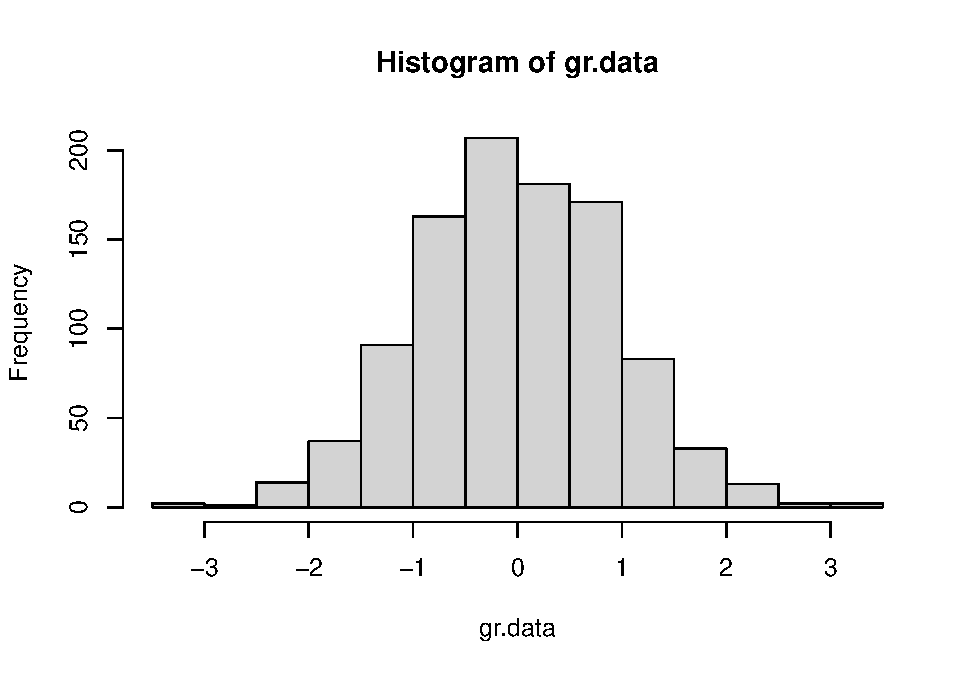
\includegraphics[keepaspectratio]{01-intro_files/figure-latex/unnamed-chunk-7-1.pdf}}

These instructions have resulted in the opening of a graph window containing the required histogram and the user can switch from the console to the graph window and back again to the console.

\begin{enumerate}
\def\labelenumi{(\alph{enumi})}
\setcounter{enumi}{10}
\tightlist
\item
  The R session can be terminated by closing the window or entering \texttt{q()} at the R prompt. Either way the user is prompted to save the \emph{{workspace}}. If the user chooses not to save, all objects created during the session are lost.
\end{enumerate}

\section{Working with RStudio}\label{working-with-rstudio}

Many users of R prefer working with \emph{{RStudio}}. \emph{{RStudio}} is a free and open source integrated development environment for R which works with the standard version of R available from CRAN. It can be downloaded from the \href{www.rstudio.com}{RStudio} home page to be run from your desktop (\emph{{Windows}}, \emph{{Mac}} or \emph{{Linux}}). Full details about the functionality of \emph{{RStudio}} are available from its home page. Here, only a brief introduction to \emph{{RStudio}} is given.

When \emph{{RStudio}} is installed on your computer the following icon is created on the desktop:

\pandocbounded{
\includegraphics[keepaspectratio]{pics/RStudio.jpg}}

Clicking the above icon open the \emph{{RStudio}} development environment as shown in Figure \ref{fig:RStudioLayout}. In order to open any R \emph{{workspace}} with \emph{{RStudio}} drag the corresponding \emph{{.RData}} file to the above \emph{{RStudio}} icon and drop it as soon as `Open with RStudio' becomes visible.

\begin{figure}
\centering
\pandocbounded{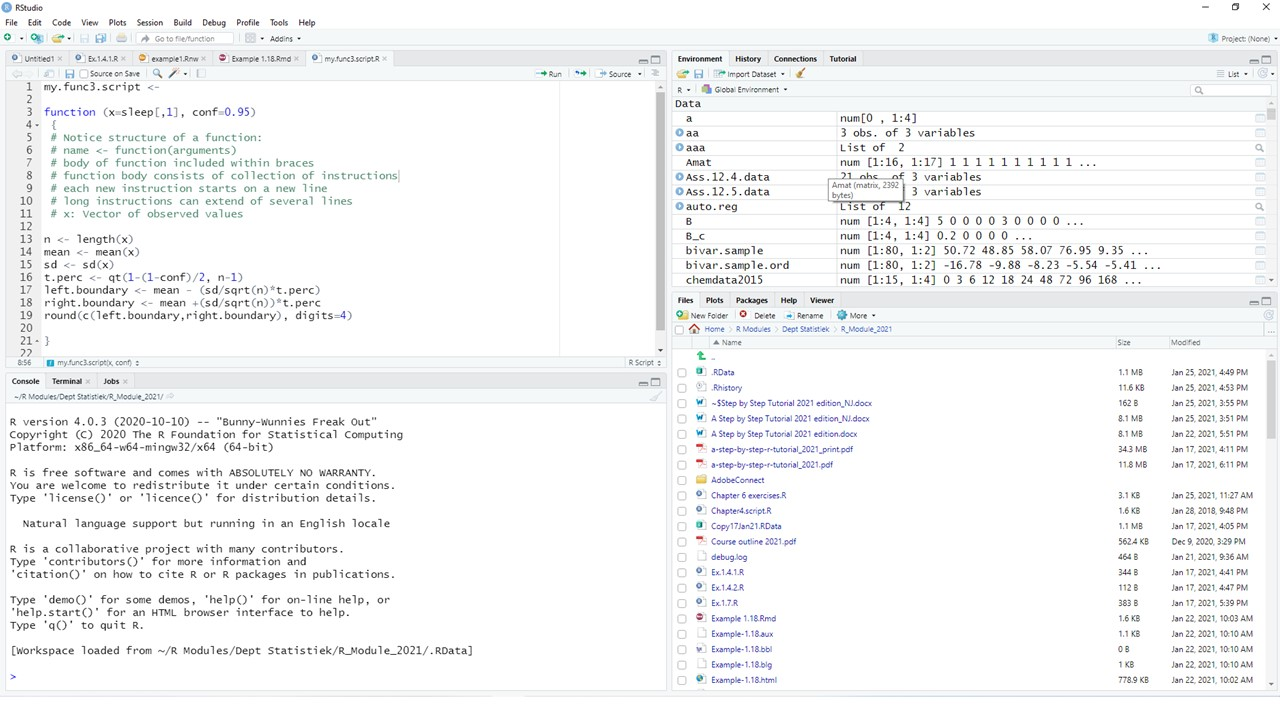
\includegraphics[keepaspectratio]{pics/RStudio_layout.jpg}}
\caption{\label{fig:RStudioLayout}The RStudio development environment for R.}
\end{figure}

The bottom left-hand panel is the familiar R console.

The bottom right-hand panel is used for :
(a) a listing of the files in the folder where the \emph{{workspace}} (\emph{{.RData}}) for the active project is kept
(b) a listing of all installed packages available to be attached to the search path as well as menus for installing and updating packages
(c) the graph windows (if any)
(d) the Help facilities.

The top left-hand panel can be used for creating and managing script files (see \ref{script}) while the top right-hand panel provides information on the objects in the current folder as well as the history of previous commands given in the console.

\section{R: an interpretive computer language}\label{r-an-interpretive-computer-language}

Essentially, in an interpretive language instructions are given one by one. Each instruction is then evaluated or interpreted in turn by an internal program called an \emph{{interpreter}} or \emph{{evaluator}} and some immediate action is taken. For example, the instruction given in \ref{QuickSample}(a) is evaluated by the R evaluator resulting in the answer \texttt{–3} being returned. On the other hand, in \ref{QuickSample}(b) the evaluator found the instruction to be incomplete and therefore asked for more information.

An advantage of an interpretive language is that intermediate results can be obtained quickly without having first to wait for a complete program to finish as is the case with a compiler language. In the latter case a complete program is translated (or compiled) by a program called a compiler. The compiled program can then be converted to a standalone application that can be called by other programs to perform a complete task. In general compiler languages handle computer memory relatively more efficiently and calculations are executed more speedily.
Communication with the R evaluator takes place through a set of instructions called \emph{{escape sequences}}. These escape sequences take the form of a backslash preceding a character. Examples of such escape sequences are:

\texttt{\textbackslash{}n} new line

\texttt{\textbackslash{}r} carriage return

\texttt{\textbackslash{}t} go to next tab stop

\texttt{\textbackslash{}b} backspace

\texttt{\textbackslash{}a} bell

\texttt{\textbackslash{}f} form feed

\texttt{\textbackslash{}v} vertical tab

A consequence of the above role of the backslash in R is that a single backslash in a filename will not be properly recognized. Therefore, when referring in R to the following file path \emph{{``c:\textbackslash My Documents\textbackslash myFile.txt''}} all backslashes must be entered as double backslashes i.e.~\texttt{"c:\textbackslash{}\textbackslash{}My\ Documents\textbackslash{}\textbackslash{}myFile.txt"} or as \texttt{"c:/My\ Documents/myFile.txt"}.

\subsection{Exercise}\label{exercise}

The \texttt{cat()} function can be used to write a text message to the console. Initialize a new R session and investigate the results of the following R instructions:

\begin{Shaded}
\begin{Highlighting}[]
\FunctionTok{cat}\NormalTok{(}\StringTok{"aaa bbb"}\NormalTok{)}
\FunctionTok{cat}\NormalTok{(}\StringTok{"aaa bbb }\SpecialCharTok{\textbackslash{}n}\StringTok{"}\NormalTok{)}
\FunctionTok{cat}\NormalTok{(}\StringTok{"aaa }\SpecialCharTok{\textbackslash{}n}\StringTok{ bbb }\SpecialCharTok{\textbackslash{}n}\StringTok{"}\NormalTok{)}
\FunctionTok{cat}\NormalTok{(}\StringTok{"aaa }\SpecialCharTok{\textbackslash{}n}\StringTok{bbb }\SpecialCharTok{\textbackslash{}n}\StringTok{"}\NormalTok{)}
\FunctionTok{cat}\NormalTok{(}\StringTok{"aaa }\SpecialCharTok{\textbackslash{}t\textbackslash{}t}\StringTok{ bbb }\SpecialCharTok{\textbackslash{}n}\StringTok{"}\NormalTok{) }
\FunctionTok{cat}\NormalTok{(}\StringTok{"aaa}\SpecialCharTok{\textbackslash{}b\textbackslash{}b\textbackslash{}b}\StringTok{bbb }\SpecialCharTok{\textbackslash{}n}\StringTok{"}\NormalTok{) }
\FunctionTok{cat}\NormalTok{(}\StringTok{"aaa }\SpecialCharTok{\textbackslash{}n\textbackslash{}a}\StringTok{ bbb }\SpecialCharTok{\textbackslash{}a\textbackslash{}n}\StringTok{"}\NormalTok{) }
\FunctionTok{cat}\NormalTok{(}\StringTok{"1}\SpecialCharTok{\textbackslash{}a\textbackslash{}n}\StringTok{"}\NormalTok{); }\FunctionTok{cat}\NormalTok{(}\StringTok{"2}\SpecialCharTok{\textbackslash{}a\textbackslash{}n}\StringTok{"}\NormalTok{)}
\end{Highlighting}
\end{Shaded}

What is the purpose of the semi-colon in the line above?

Could you distinguish the two soundings of the bell? Try the following:

\begin{Shaded}
\begin{Highlighting}[]
\FunctionTok{cat}\NormalTok{(}\StringTok{"1}\SpecialCharTok{\textbackslash{}a\textbackslash{}n}\StringTok{"}\NormalTok{); }\FunctionTok{Sys.sleep}\NormalTok{(}\DecValTok{2}\NormalTok{); }\FunctionTok{cat}\NormalTok{(}\StringTok{"2}\SpecialCharTok{\textbackslash{}a\textbackslash{}n}\StringTok{"}\NormalTok{) }
\end{Highlighting}
\end{Shaded}

Could you now distinguish the two soundings of the bell?

What is the purpose of the \texttt{Sys.sleep()} instruction?

\subsection{Exercise}\label{exercise-1}

Write R code to achieve the following output:

\texttt{My\ name\ is:}

Bell sounds once.

Your name appears on a new line.

Two distinct sounds of the bell are heard and

\texttt{Thank\ you} is visible on a new line.

The cursor appears on a new line.

\section{Accessing the Help functionality}\label{accessing-the-help-functionality}

\begin{enumerate}
\def\labelenumi{(\alph{enumi})}
\tightlist
\item
  Use
\end{enumerate}

\begin{Shaded}
\begin{Highlighting}[]
\NormalTok{?mean}
\end{Highlighting}
\end{Shaded}

to obtain help on the usage of the R function \texttt{mean()}.

\begin{enumerate}
\def\labelenumi{(\alph{enumi})}
\setcounter{enumi}{1}
\tightlist
\item
  Find out what is the difference between the instructions
\end{enumerate}

\begin{Shaded}
\begin{Highlighting}[]
\NormalTok{?mean}
\end{Highlighting}
\end{Shaded}

and

\begin{Shaded}
\begin{Highlighting}[]
\NormalTok{??mean}
\end{Highlighting}
\end{Shaded}

\begin{enumerate}
\def\labelenumi{(\alph{enumi})}
\setcounter{enumi}{2}
\tightlist
\item
  What help is available via the instruction
\end{enumerate}

\begin{Shaded}
\begin{Highlighting}[]
\FunctionTok{help.start}\NormalTok{()}
\end{Highlighting}
\end{Shaded}

\begin{enumerate}
\def\labelenumi{(\alph{enumi})}
\setcounter{enumi}{3}
\tightlist
\item
  Use
\end{enumerate}

\begin{Shaded}
\begin{Highlighting}[]
\NormalTok{?}\FunctionTok{help.search}\NormalTok{()}
\end{Highlighting}
\end{Shaded}

to find out how to obtain help using the R function \texttt{help.search(xx)}. Note: For hep on an operator or reserved word quotes are needed, e.g.

\begin{Shaded}
\begin{Highlighting}[]
\NormalTok{?matrix}
\end{Highlighting}
\end{Shaded}

but

\begin{Shaded}
\begin{Highlighting}[]
\NormalTok{?}\StringTok{"?"}
\end{Highlighting}
\end{Shaded}

or

\begin{Shaded}
\begin{Highlighting}[]
\NormalTok{?}\StringTok{"for"}
\end{Highlighting}
\end{Shaded}

\section{More R basics}\label{MoreBasics}

\begin{enumerate}
\def\labelenumi{(\alph{enumi})}
\item
  R as an \emph{{interactive}} language allows for fast acquisition of results.
\item
  R is a \emph{{functional}} language in two important senses: In a more technical sense it means the R model of computation relies more on \emph{{function evaluation}} than by procedural computations and changes of state. The second sense refers to the way how users communicate to R namely almost entirely through \emph{{function calls}}.
\item
  R as an \emph{{object-oriented}} language refers in a technical sense to the S4 or S5 type of objects with their associated classes and methods as mentioned in the Preface. In a less technical sense it means that everything in R is an object.
\item
  R objects will be studied in detail in later chapters. What is important for now, is the following:
\end{enumerate}

\begin{itemize}
\tightlist
\item
  Everything in R is an object.
\item
  There are different types of objects e.g.~function objects, data objects, graphics objects, character objects, numeric objects.
\item
  Usually objects are stored in the current folder called the \emph{{Global environment}}; recognized by R under the name \texttt{.GlobalEnv} and available in the file system under the name \emph{{.RData}}.
\item
  Objects are created from the console by \emph{{assignment}} through the instruction
\end{itemize}

\begin{Shaded}
\begin{Highlighting}[]
\NormalTok{name }\OtherTok{\textless{}{-}}\NormalTok{ object}
\end{Highlighting}
\end{Shaded}

or

\begin{Shaded}
\begin{Highlighting}[]
\NormalTok{object }\OtherTok{\textless{}{-}}\NormalTok{ name}
\end{Highlighting}
\end{Shaded}

\begin{itemize}
\tightlist
\item
  In R names are \emph{{case sensitive}} i.e.~peter and Peter are two different objects.
\item
  Objects created by assignment during an R session are stored permanently in the Global environment (working directory) unless the user chooses not to save when terminating an R session.
\item
  Care must be exercised when creating a new object by assignment: if an object with the name my.object already exists in the Global environment and a new object is created by assigning it to the name my.object then the old my.object is over-written and it is replaced by the new object \emph{{without any warning}}.
\item
  Remember the way the R evaluator operates: if an object name is given at the R prompt the R evaluator responds by displaying the content of the object. Review the difference between the instructions
\end{itemize}

\begin{Shaded}
\begin{Highlighting}[]
\NormalTok{q}
\end{Highlighting}
\end{Shaded}

and

\begin{Shaded}
\begin{Highlighting}[]
\FunctionTok{q}\NormalTok{()}
\end{Highlighting}
\end{Shaded}

\begin{enumerate}
\def\labelenumi{(\alph{enumi})}
\setcounter{enumi}{4}
\tightlist
\item
  The symbol \texttt{\#} marks a comment. Everything following a \texttt{\#} on a line is ignored by the R evaluator. Check for example the result of the instruction
\end{enumerate}

\begin{Shaded}
\begin{Highlighting}[]
\DecValTok{5}\SpecialCharTok{+}\DecValTok{8} \CommentTok{\# +12}
\CommentTok{\#\textgreater{} [1] 13}
\end{Highlighting}
\end{Shaded}

\begin{enumerate}
\def\labelenumi{(\alph{enumi})}
\setcounter{enumi}{5}
\item
  Usage of the symbols \texttt{\textless{}-}, \texttt{=} and \texttt{==}. The symbol \texttt{\textless{}-} is used for assigning the object on its right-hand side to a name (label) on its left-hand side; the equality sign \texttt{=} is used for specifying the arguments of functions while the double equality symbol \texttt{==} is used for comparison purposes. In earlier versions of R these rules were strictly applied by the R evaluator. However, in recent versions of R the evaluator allows the equality sign also in the case for assigning an object to a name. We believe that reserving the equality sign only for argument specifications in functions leads to more clarity when writing complex functions and therefore we discourage its usage for creating objects by assignment. In this book creating objects by assignment will be exclusively carried out with the assignment symbol \texttt{\textless{}-}.
\item
  The symbol \texttt{-\textgreater{}} assigns the object on its left-hand side to the name (label) on its right-hand side.
\item
  Working with packages: The core installation includes several packages. To see them issue the command \texttt{search()} from the R prompt in the console. Notice that the first object in the search list is \texttt{.GlobalEnv}. This is followed by other objects. Packages are recognized by the string package followed by a colon and the name of the package. In order for a package to be used the following steps must be followed: if the package has been \emph{{installed}} previously it needs only to be \emph{{loaded}} into the search path using the command \texttt{library(packagename)} from the R prompt. This will load the package by default in the second position on the search path. If the package has not been installed previously it must first be installed. This is most easily done using the top menu Packages. The command \texttt{require(packagename)} appears to be identical to \texttt{library(packagename)}. The function \texttt{require()} is designed for use inside other functions as it gives a warning, rather than an error, if the package does not exist.
\item
  More on the help (\texttt{?}) facility: Table \ref{tab:HelpQueries} contains details about help available for some special keywords.
\end{enumerate}

\begin{longtable}[]{@{}
  >{\raggedright\arraybackslash}p{(\linewidth - 2\tabcolsep) * \real{0.2857}}
  >{\raggedright\arraybackslash}p{(\linewidth - 2\tabcolsep) * \real{0.7143}}@{}}
\caption{\label{tab:HelpQueries} Some useful keywords available for help queries.}\tabularnewline
\toprule\noalign{}
\begin{minipage}[b]{\linewidth}\raggedright
\emph{{Help query}}
\end{minipage} & \begin{minipage}[b]{\linewidth}\raggedright
\emph{{Explanation}}
\end{minipage} \\
\midrule\noalign{}
\endfirsthead
\toprule\noalign{}
\begin{minipage}[b]{\linewidth}\raggedright
\emph{{Help query}}
\end{minipage} & \begin{minipage}[b]{\linewidth}\raggedright
\emph{{Explanation}}
\end{minipage} \\
\midrule\noalign{}
\endhead
\bottomrule\noalign{}
\endlastfoot
\texttt{?Arithmetic} & Unary and binary operators to perform arithmetic on numeric and complex vectors \\
\texttt{?Comparison} & Binary operators for comparison of values in vectors \\
\texttt{?Control} & The basic constructs for control of the flow in R instructions \\
\texttt{?dotsMethods} & The use of the special operator \texttt{...} \\
\texttt{?Extract} & Operators to extract or replace parts of vectors, matrices, arrays and lists \\
\texttt{?Logic} & Logical operators for operating on logical and numeric vectors \\
\texttt{?.Machine} & Information on the variable \texttt{.Machine} holding information on the numerical characteristics of the machine R is running on \\
\texttt{?NumericConstants} & How R parses numeric constants including \texttt{Inf}, \texttt{NaN}, \texttt{NA} \\
\texttt{?options} & Allow the user to set and examine a variety of global options which affect the way in which R computes and displays its results \\
\texttt{?Paren} & Parentheses and braces in R \\
\texttt{?Quotes} & Single and double quotation marks. Back quote (backtick) and backslash for starting an escape sequence \\
\texttt{?Reserved} & Description of reserved words in R \\
\texttt{?Special} & Special mathematical functions related to the beta and gamma functions including permutations and combinations \\
\texttt{?Syntax} & Outlines R syntax and gives the precedence of operators \\
\end{longtable}

\section{Regular expressions in R: the basics}\label{regular-expressions-in-r-the-basics}

It follows from \ref{MoreBasics}(d) that care must be taken when objects are assigned to names. Furthermore, the Global environment or any other R database may easily contain hundreds of objects. Therefore, a frequent task is to search for patterns in the names of objects e.g.~searching for all object names starting with ``Figure'' or ending in ``.dat''. The R function \texttt{objects()} or \texttt{ls()} has arguments \texttt{pos} and \texttt{pattern} for specifying the position of a database to search and a pattern of characters appearing in a name (or string), respectively. The pattern argument can be given any \emph{{regular expression}}. Regular expressions provide a method of expressing patterns in character values and are used to perform various tasks in R. Here we are only considering the task of extracting certain specified objects in a database using the pattern argument of \texttt{objects()} or \texttt{ls()}.

The syntax of regular expressions follows different rules to the syntax of ordinary R instructions. Moreover its syntax differs depending on the particular implementation a program uses. By default, R uses a set of regular expressions similar to those used by UNIX utilities, but function arguments are available for changing the default e.g.~by setting argument \texttt{perl\ =\ TRUE}.

Regular expressions consist of three components: \emph{{single characters}}, \emph{{character classes}} and \emph{{modifiers}} operating on single characters and character classes.

Character classes are formed by using square brackets surrounding a set of characters to be matched e.g.~\texttt{{[}abc123{]}}, \texttt{{[}a-z{]}}, \texttt{{[}a-zA-Z{]}}, \texttt{{[}0-9a-z{]}}. Note the usage of the dash to indicate a range of values.

The modifiers operating on characters or character classes are summarized in Table \ref{tab:RegExprMod}.

\begin{longtable}[]{@{}
  >{\raggedright\arraybackslash}p{(\linewidth - 2\tabcolsep) * \real{0.2857}}
  >{\raggedright\arraybackslash}p{(\linewidth - 2\tabcolsep) * \real{0.7143}}@{}}
\caption{\label{tab:RegExprMod} Modifiers for regular expressions.}\tabularnewline
\toprule\noalign{}
\begin{minipage}[b]{\linewidth}\raggedright
\emph{{Modifier}}
\end{minipage} & \begin{minipage}[b]{\linewidth}\raggedright
\emph{{Operation}}
\end{minipage} \\
\midrule\noalign{}
\endfirsthead
\toprule\noalign{}
\begin{minipage}[b]{\linewidth}\raggedright
\emph{{Modifier}}
\end{minipage} & \begin{minipage}[b]{\linewidth}\raggedright
\emph{{Operation}}
\end{minipage} \\
\midrule\noalign{}
\endhead
\bottomrule\noalign{}
\endlastfoot
\texttt{\^{}} & Expression anchors at beginning of target string \\
\texttt{\$} & Expression anchors at end of target string \\
\texttt{.} & Any single character except newline is matched \\
\texttt{\textbar{}} & Alternative patterns are separated \\
\texttt{(\ )} & Patterns are grouped together \\
\texttt{*} & Zero or more occurrences of preceding entity are matched \\
\texttt{?} & Zero or one occurrences of preceding entity are matched \\
\texttt{+} & One or more occurrences of preceding entity are matched \\
\texttt{\{n\}} & Exactly n occurrences of preceding entity are matched \\
\texttt{\{n,\}} & At least n occurrences of preceding entity are matched \\
\texttt{\{n,\ m\}} & At least n and at most m occurrences of preceding entity are matched \\
\end{longtable}

Because of their role as modifiers or in forming character classes the following characters must be preceded by a backslash when their literal meaning is needed:

\begin{verbatim}
[  ]  {  }  (  )  ^  $  .  |  *  +  \
\end{verbatim}

Note that in R this means that whenever one of the above characters needs to be escaped in a regular expression it must be preceded by double backslashes. Table \ref{tab:RegExpr} contains some examples of regular expressions.

\begin{longtable}[]{@{}
  >{\raggedright\arraybackslash}p{(\linewidth - 2\tabcolsep) * \real{0.2857}}
  >{\raggedright\arraybackslash}p{(\linewidth - 2\tabcolsep) * \real{0.7143}}@{}}
\caption{\label{tab:RegExpr} Examples of regular expressions.}\tabularnewline
\toprule\noalign{}
\begin{minipage}[b]{\linewidth}\raggedright
\emph{{Regular expression}}
\end{minipage} & \begin{minipage}[b]{\linewidth}\raggedright
\emph{{Meaning}}
\end{minipage} \\
\midrule\noalign{}
\endfirsthead
\toprule\noalign{}
\begin{minipage}[b]{\linewidth}\raggedright
\emph{{Regular expression}}
\end{minipage} & \begin{minipage}[b]{\linewidth}\raggedright
\emph{{Meaning}}
\end{minipage} \\
\midrule\noalign{}
\endhead
\bottomrule\noalign{}
\endlastfoot
\texttt{"{[}a-z{]}{[}a-z{]}{[}0-9{]}"} & Matches a string consisting of two lower case letters followed by a digit \\
\texttt{"{[}a-z{]}{[}a-z{]}{[}0-9{]}\$"} & Matches a string ending in two lower case letters followed by a digit \\
\texttt{"\^{}{[}a-zA-Z{]}+\textbackslash{}\textbackslash{}."} & Matches a string beginning with any number of lower or upper case letters followed by a period \\
\texttt{"(ab)\{2\}(34)\{2\}\$"} & Matches a string ending in \texttt{abab3434} \\
\end{longtable}

\subsection{Exercise}\label{exercise-2}

Initialize an R session

\begin{enumerate}
\def\labelenumi{(\alph{enumi})}
\tightlist
\item
  Attach the MASS package in the second (the default) position on the search path by issuing the command
\end{enumerate}

\begin{Shaded}
\begin{Highlighting}[]
\FunctionTok{library}\NormalTok{(MASS)}
\end{Highlighting}
\end{Shaded}

\begin{enumerate}
\def\labelenumi{(\alph{enumi})}
\setcounter{enumi}{1}
\tightlist
\item
  Get a listing of all the objects in package MASS by requesting
\end{enumerate}

\begin{Shaded}
\begin{Highlighting}[]
\FunctionTok{objects}\NormalTok{(}\AttributeTok{pos=}\DecValTok{2}\NormalTok{)}
\end{Highlighting}
\end{Shaded}

\begin{enumerate}
\def\labelenumi{(\alph{enumi})}
\setcounter{enumi}{2}
\tightlist
\item
  Explain the difference between \texttt{objects(pos=2,\ pat=".")} and \texttt{objects(pos=2,\ patt="\textbackslash{}\textbackslash{}.")}.
\item
  Obtain a listing of all objects with names starting with three letters followed by a digit.
\item
  Obtain a listing of all objects with names ending with three letters followed by a digit.
\item
  Obtain a listing of all objects with names ending in a period followed by exactly three or four letters.
\end{enumerate}

\section{From single instructions to sets of instructions: introducing R functions}\label{FunctionIntro}

Consider the following problem: the R data set \texttt{sleep} contains the extra hours of sleep of 20 patients after a drug treatment. Suppose this data set can be considered a sample from a normal population. A 95\% confidence interval is required for the mean extra hours of sleep. It is known that the confidence interval is given by \(\left[ \mathbf{\bar{x}}- \left( \frac{s}{\sqrt(n)} \right) t_{n-1,0.025}; \mathbf{\bar{x}}+ \left( \frac{s}{\sqrt(n)} \right) t_{n-1,0.025} \right]\). This problem can be solved by entering the following instructions one by one:

\begin{Shaded}
\begin{Highlighting}[]
\NormalTok{sleep.data }\OtherTok{\textless{}{-}}\NormalTok{ sleep[ ,}\DecValTok{1}\NormalTok{]   }
\NormalTok{sleep.mean }\OtherTok{\textless{}{-}} \FunctionTok{mean}\NormalTok{(sleep.data)   }
\NormalTok{sleep.sd }\OtherTok{\textless{}{-}} \FunctionTok{sd}\NormalTok{(sleep.data)    }
\NormalTok{t.perc }\OtherTok{\textless{}{-}} \FunctionTok{qt}\NormalTok{(}\FloatTok{0.975}\NormalTok{,}\DecValTok{19}\NormalTok{) }
\NormalTok{left.boundary }\OtherTok{\textless{}{-}}\NormalTok{ sleep.mean }\SpecialCharTok{{-}}\NormalTok{ (sleep.sd}\SpecialCharTok{/}\FunctionTok{sqrt}\NormalTok{(}\FunctionTok{length}\NormalTok{(sleep.data)))}\SpecialCharTok{*}\NormalTok{t.perc }
\NormalTok{right.boundary }\OtherTok{\textless{}{-}}\NormalTok{ sleep.mean }\SpecialCharTok{+}\NormalTok{ (sleep.sd}\SpecialCharTok{/}\FunctionTok{sqrt}\NormalTok{(}\FunctionTok{length}\NormalTok{(sleep.data)))}\SpecialCharTok{*}\NormalTok{t.perc}
\FunctionTok{cat}\NormalTok{ (}\StringTok{"["}\NormalTok{, left.boundary, }\StringTok{";"}\NormalTok{, right.boundary, }\StringTok{"]}\SpecialCharTok{\textbackslash{}n}\StringTok{"}\NormalTok{)}
\CommentTok{\#\textgreater{} [ 0.5955845 ; 2.484416 ]}
\end{Highlighting}
\end{Shaded}

In situations like the above, the problem can be addressed using a \emph{{script file}} or writing a \emph{{function}}. We are going to introduce two methods for writing functions in R:

\begin{enumerate}
\def\labelenumi{(\roman{enumi})}
\tightlist
\item
  using a script file and
\item
  using the function \texttt{fix()}.
\end{enumerate}

\subsection{Writing an R function using a script file}\label{script}

\begin{enumerate}
\def\labelenumi{(\alph{enumi})}
\tightlist
\item
  From the R top menu select \emph{File; New script}. A script window will open with a simultaneous change in the menu bar.
\item
  Type the instructions in the script window.
\item
  Select all the typed text and run the script by clicking the run icon (or Ctrl+R).
\item
  Note what is shown in the R console window.
\item
  Script files are ordinary text files. They can be saved, edited and opened using any text editor.
\item
  By convention R script files have the extension {xxxx.r}.
\item
  Next, change the spelling in the last two lines from \texttt{right.boundary} to \texttt{Right.boundary}. Select all the text and run the script. Check the output appearing on the console.
\item
  Script windows can also be used for creating an R function.
\item
  Create an R function by changing the text as shown below.
\end{enumerate}

\begin{Shaded}
\begin{Highlighting}[]
\NormalTok{conf.int }\OtherTok{\textless{}{-}} \ControlFlowTok{function}\NormalTok{ (}\AttributeTok{x =}\NormalTok{ sleep[,}\DecValTok{1}\NormalTok{])}
\NormalTok{\{}
\NormalTok{  x.mean }\OtherTok{\textless{}{-}} \FunctionTok{mean}\NormalTok{(x)   }
\NormalTok{  x.sd }\OtherTok{\textless{}{-}} \FunctionTok{sd}\NormalTok{(x)    }
\NormalTok{  t.perc }\OtherTok{\textless{}{-}} \FunctionTok{qt}\NormalTok{(}\FloatTok{0.975}\NormalTok{,}\DecValTok{19}\NormalTok{) }
\NormalTok{  left.boundary }\OtherTok{\textless{}{-}}\NormalTok{ x.mean }\SpecialCharTok{{-}}\NormalTok{ (x.sd}\SpecialCharTok{/}\FunctionTok{sqrt}\NormalTok{(}\FunctionTok{length}\NormalTok{(x)))}\SpecialCharTok{*}\NormalTok{t.perc }
\NormalTok{  right.boundary }\OtherTok{\textless{}{-}}\NormalTok{ x.mean }\SpecialCharTok{+}\NormalTok{ (x.sd}\SpecialCharTok{/}\FunctionTok{sqrt}\NormalTok{(}\FunctionTok{length}\NormalTok{(x)))}\SpecialCharTok{*}\NormalTok{t.perc}
  \FunctionTok{list}\NormalTok{ (}\AttributeTok{lower =}\NormalTok{ left.boundary, }\AttributeTok{upper =}\NormalTok{ right.boundary)  }
\NormalTok{\}}
\end{Highlighting}
\end{Shaded}

\begin{enumerate}
\def\labelenumi{(\alph{enumi})}
\setcounter{enumi}{9}
\tightlist
\item
  Select the text and notice what happens in the R commands window (the console).
\item
  Give the instruction \texttt{objects()} at the R prompt. What has happened?
\item
  You can now run the function from the commands window (the console) by typing:
\end{enumerate}

\begin{Shaded}
\begin{Highlighting}[]
\FunctionTok{conf.int}\NormalTok{ (}\AttributeTok{x =}\NormalTok{ sleep[,}\DecValTok{1}\NormalTok{])}
\CommentTok{\#\textgreater{} $lower}
\CommentTok{\#\textgreater{} [1] 0.5955845}
\CommentTok{\#\textgreater{} }
\CommentTok{\#\textgreater{} $upper}
\CommentTok{\#\textgreater{} [1] 2.484416}
\end{Highlighting}
\end{Shaded}

\begin{enumerate}
\def\labelenumi{(\alph{enumi})}
\setcounter{enumi}{11}
\tightlist
\item
  If you want to create and run the function \texttt{conf.int} in a script window then add the instruction \texttt{conf.func\ (x\ =\ sleep{[},1{]})} as the last line in the script window. Now, select only this line and run it. Check the R console.
\item
  What will happen if a syntax error is made in the script window? Change the code in the script file as follows, deliberately deleting the last closing parenthesis in the last line of the function.
\end{enumerate}

\begin{Shaded}
\begin{Highlighting}[]
\NormalTok{conf.int }\OtherTok{\textless{}{-}} \ControlFlowTok{function}\NormalTok{ (}\AttributeTok{x =}\NormalTok{ sleep[,}\DecValTok{1}\NormalTok{])}
\NormalTok{\{}
\NormalTok{  x.mean }\OtherTok{\textless{}{-}} \FunctionTok{mean}\NormalTok{(x)   }
\NormalTok{  x.sd }\OtherTok{\textless{}{-}} \FunctionTok{sd}\NormalTok{(x)    }
\NormalTok{  t.perc }\OtherTok{\textless{}{-}} \FunctionTok{qt}\NormalTok{(}\FloatTok{0.975}\NormalTok{,}\DecValTok{19}\NormalTok{) }
\NormalTok{  left.boundary }\OtherTok{\textless{}{-}}\NormalTok{ x.mean }\SpecialCharTok{{-}}\NormalTok{ (x.sd}\SpecialCharTok{/}\FunctionTok{sqrt}\NormalTok{(}\FunctionTok{length}\NormalTok{(x)))}\SpecialCharTok{*}\NormalTok{t.perc }
\NormalTok{  right.boundary }\OtherTok{\textless{}{-}}\NormalTok{ x.mean }\SpecialCharTok{+}\NormalTok{ (x.sd}\SpecialCharTok{/}\FunctionTok{sqrt}\NormalTok{(}\FunctionTok{length}\NormalTok{(x)))}\SpecialCharTok{*}\NormalTok{t.perc}
  \FunctionTok{list}\NormalTok{ (}\AttributeTok{lower =}\NormalTok{ left.boundary, }\AttributeTok{upper =}\NormalTok{ right.boundary}
\ErrorTok{\}}
\FunctionTok{conf.int}\NormalTok{ (}\AttributeTok{x =}\NormalTok{ sleep[,}\DecValTok{1}\NormalTok{])}
\end{Highlighting}
\end{Shaded}

\begin{enumerate}
\def\labelenumi{(\alph{enumi})}
\setcounter{enumi}{13}
\tightlist
\item
  Select \emph{only the final line} and run it. Check the R console. No problem, the function executed correctly. This is because the code for \texttt{conf.int} in the script file was changed, but the updated object was not created by running it in the console.
\item
  Select \emph{all the code} in the script and run it. Check the R console. Discuss.
\end{enumerate}

\subsection{\texorpdfstring{Writing an R function using \texttt{fix()}}{Writing an R function using fix()}}\label{writing-an-r-function-using-fix}

When using \texttt{fix()} the built-in \emph{{R text editor}} can be used when using script files but in the windows environment {notepad} or preferably \href{www.notepad-plus-plus.org/download/}{notepad++} or \href{https://tinn-r.org/en/}{Tinn-R} is preferred.

The following instruction is necessary for changing the default editor to be used with \texttt{fix()}:

\begin{Shaded}
\begin{Highlighting}[]
\FunctionTok{options}\NormalTok{(}\AttributeTok{editor =} \StringTok{"notepad"}\NormalTok{)}
\end{Highlighting}
\end{Shaded}

or

\begin{Shaded}
\begin{Highlighting}[]
\FunctionTok{options}\NormalTok{(}\AttributeTok{editor =} \StringTok{"full path to the relevant exe file"}\NormalTok{)}
\end{Highlighting}
\end{Shaded}

\begin{enumerate}
\def\labelenumi{(\alph{enumi})}
\tightlist
\item
  Enter \texttt{fix\ (my.func)} at the R prompt. A text editor will open. Type the instructions as shown below.
\end{enumerate}

\begin{Shaded}
\begin{Highlighting}[]
\NormalTok{function (x = sleep[,1])}
\NormalTok{\{}
\NormalTok{  x.mean \textless{}{-} mean(x)\textasciigrave{}}
\NormalTok{  x.sd \textless{}{-} sd(x)}
\NormalTok{  t.perc \textless{}{-} qt(0.975,19)}
\NormalTok{  left.boundary \textless{}{-} x.mean {-} (x.sd/sqrt(length(x)))*t.perc}
\NormalTok{  right.boundary \textless{}{-} x.mean + (x.sd/sqrt(length(x)))*t.perc}
\NormalTok{  list (lower = left.boundary, upper = right.boundary)}
\NormalTok{\}}
\end{Highlighting}
\end{Shaded}

Close the window. Check what happens in the R console.

You can now run the function from the commands window (the console) similar to in \ref{script}(l), but changing the name of the function from \texttt{conf.int} to \texttt{my.func}.

\begin{enumerate}
\def\labelenumi{(\alph{enumi})}
\setcounter{enumi}{1}
\item
  What will happen if a syntax error is made when using fix? At the R prompt type \texttt{fix\ (my.func)}. Make a deliberate syntax error, e.g.~delete the last closing brace. Close the text editor window. What happens in the console? What is to be done to correct the mistake?
\item
  Carefully study the message in the R console when a syntax error occurred in a function created by \texttt{fix()}:
\end{enumerate}

\begin{Shaded}
\begin{Highlighting}[]
\NormalTok{\textgreater{} Error in edit(name, file, title, editor) :}
\NormalTok{    unexpected \textquotesingle{}yyy\textquotesingle{} occurred on line xx}
\NormalTok{    use a command like}
\NormalTok{    x \textless{}{-} edit()}
\NormalTok{    to recover}
\end{Highlighting}
\end{Shaded}

\begin{enumerate}
\def\labelenumi{(\alph{enumi})}
\setcounter{enumi}{3}
\tightlist
\item
  The following is the correct way to respond to the above message from the R evaluator:
\end{enumerate}

\begin{Shaded}
\begin{Highlighting}[]
\NormalTok{my.func }\OtherTok{\textless{}{-}} \FunctionTok{edit}\NormalTok{()}
\end{Highlighting}
\end{Shaded}

If you simply use \texttt{fix(my.func)} at this point, the R and the editor will revert to the version of the function \emph{before} the previous edit.

\textbf{WARNING}

Before writing a function for solving any problem: make sure the problem is understood exactly; make 100\% sure the relevant statistical theory is understood correctly. Failure to do so is careless and dangerous!

\section{R Projects}\label{r-projects}

The different windows in R are the Data window, Script window, Graph window and Menus and Dialog windows. The current \emph{{workspace}} in R is \texttt{.GlobalEnv}. The function \texttt{getwd()} is used to obtain the path to the current folder's \emph{{.Rdata}} and \emph{{.Rhistory}}.

\emph{Note}: In order to see the files \emph{{.Rdata}} and \emph{{.Rhistory}} being displayed as such, it may be necessary to turn off the option ``Hide extensions for known file types'' in \emph{{Windows Explorer}}.

It is important to make provision for different \emph{{workspaces}} associated with different \emph{{projects}}. In R, different \emph{{.Rdata}} files in different folders would separate different projects. There is however much to gain in using \emph{Projects} in \emph{{RStudio}}.

\subsection{Creating a project in RStudio}\label{creating-a-project-in-rstudio}

From the top menu, select \emph{File, New Project}. Follow the prompts to create a new project, either in an existing folder or creating a new folder for your project, say \emph{{MyProject}}.

\begin{enumerate}
\def\labelenumi{(\alph{enumi})}
\item
  Navigate to the folder \emph{{MyProject}} in \emph{{Windows Explorer}}.
\item
  Notice a file \emph{{MyProject.Rproj}} has been created in the folder.
\item
  By double-clicking on this file you open the project in \emph{{RStudio}}. The advantages of opening the project this way are:
\end{enumerate}

\begin{itemize}
\item
  your \emph{{workspace}} from the file \emph{{MyProject.Rdata}} is automatically loaded
\item
  by placing any related files like data set in the folder \emph{{MyProject}} or a subfolder, say \emph{{MyProject\textbackslash data}} means that in your code you only have to use relative folder references, i.e.~refer to \emph{{MyProject\textbackslash mydata.xlsx}} or \emph{{MyProject\textbackslash data\textbackslash mydata.xlsx}} instead of something like \emph{{c:\textbackslash users\textbackslash myname\textbackslash Documents\textbackslash MyProject\textbackslash data\textbackslash mydata.xlsx}}.
\item
  the major advantage of relative references is that it is not specific to the computer and makes porting between devices possible
\item
  sharing your project with a collaborator will simply entail copying the entire contents of the \emph{{MyProject}} folder.
\end{itemize}

\section{A note on computations by a computer}\label{a-note-on-computations-by-a-computer}

When writing R functions it is important to keep in mind that the way computations are performed by a computer are not always according to the rules of algebra. Two important occurrences are given below.

\begin{itemize}
\item
  In mathematics the following statement is incorrect: \texttt{x\ =\ x\ +\ k} for \(k \neq 0\) but in computer programming the statement \texttt{x\ =\ x\ +\ k} is legitimate and it means \texttt{x} is replaced by \texttt{x\ +\ k}.
\item
  In general, the treatment of integers and real numbers for which R uses floating point representation happens at a fundamental level over which R has no control. Real numbers cannot necessarily be exactly represented in a computer -- some can only be approximated. Furthermore, there are limitations to the minimum and maximum numbers that can be represented in a computer. This might lead to what is known as \emph{{underflow}} or \emph{{overflow}}. A more detailed discussion appears in a later chapter.
\end{itemize}

Open an R session and issue the command

\begin{Shaded}
\begin{Highlighting}[]
\NormalTok{.Machine}
\end{Highlighting}
\end{Shaded}

for details about the numerical environment of your computer.

\section{Built-in data sets in R}\label{built-in-data-sets-in-r}

R contains several built-in data sets collected in the package \texttt{datasets}. This package is automatically attached to the search path. Type \texttt{?datasets} at the R prompt for details. Apart from these data sets several other data sets from other packages are also used in this book.

\section{\texorpdfstring{The use of \texttt{.First()} and \texttt{.Last()}}{The use of .First() and .Last()}}\label{the-use-of-.first-and-.last}

The function \texttt{.First()} is executed at the beginning of every R session. \emph{{This only works in R and not in RStudio}}.

Instead of having to specify

\begin{Shaded}
\begin{Highlighting}[]
\FunctionTok{options}\NormalTok{(}\AttributeTok{editor =} \StringTok{"notepad"}\NormalTok{)}
\end{Highlighting}
\end{Shaded}

each time an R session is initialized, create the following function and save in the {.Rdata} before exiting R.

\begin{Shaded}
\begin{Highlighting}[]
\NormalTok{.First }\OtherTok{\textless{}{-}} \ControlFlowTok{function}\NormalTok{() \{ }\FunctionTok{options}\NormalTok{(}\AttributeTok{editor =} \StringTok{"notepad"}\NormalTok{) \}}
\end{Highlighting}
\end{Shaded}

to ensures that Notepad is the text editor during any subsequent session.

Similar to \texttt{.First()} the function \texttt{.Last()} can be created for execution at the end of an R session.

\subsection{\texorpdfstring{Security: an example of the usage of \texttt{.First()}}{Security: an example of the usage of .First()}}\label{security-an-example-of-the-usage-of-.first}

The \texttt{.First()} facility can be used to prevent access to a R \emph{{workspace}} by setting a password protection. This can be done as follows:

Create a new \emph{{workspace}} for running the example on security. In this \emph{{workspace}} create the following R function

\begin{Shaded}
\begin{Highlighting}[]
\NormalTok{password }\OtherTok{\textless{}{-}} \ControlFlowTok{function}\NormalTok{()        }\CommentTok{\# Note the structure of a function}
\NormalTok{\{ }\FunctionTok{cat}\NormalTok{(}\StringTok{"Password? }\SpecialCharTok{\textbackslash{}n}\StringTok{"}\NormalTok{)}
\NormalTok{  password }\OtherTok{\textless{}{-}} \FunctionTok{readline}\NormalTok{()      }\CommentTok{\# What is the usage of readline()? }
  \ControlFlowTok{if}\NormalTok{ (password }\SpecialCharTok{!=} \StringTok{"PASSWORD"}\NormalTok{) }
    \FunctionTok{q}\NormalTok{(}\AttributeTok{save=}\StringTok{"no"}\NormalTok{)              }\CommentTok{\# The meaning of !=  is "not equal to"}
  \ControlFlowTok{else}\NormalTok{ (}\FunctionTok{cat}\NormalTok{(}\StringTok{"You can proceed }\SpecialCharTok{\textbackslash{}n}\StringTok{"}\NormalTok{))}
\NormalTok{\}               }
\end{Highlighting}
\end{Shaded}

Now create the function:

\begin{Shaded}
\begin{Highlighting}[]
\NormalTok{.First }\OtherTok{\textless{}{-}} \ControlFlowTok{function}\NormalTok{()}
\NormalTok{\{   }\CommentTok{\#  What must you be careful of?}
   \FunctionTok{password}\NormalTok{()}
\NormalTok{\}}
\end{Highlighting}
\end{Shaded}

\begin{itemize}
\tightlist
\item
  Terminate your R session and open it again.
\item
  Discuss the construction and usage of the above functions.
\item
  Can you break the above security?
\item
  Can you make changes to the above security to make it more safe?
\end{itemize}

\section{Options}\label{options}

Study the result of the instruction \texttt{\textgreater{}\ options()} in R.

\section{Creating PDF and HTML documents from R output: R Markdown}\label{creating-pdf-and-html-documents-from-r-output-r-markdown}

The R package \texttt{knitr} is used to obtain reproducible results from R code in the form of \emph{{.pdf}} or \emph{{.html}} documents. In addition to \texttt{knitr}, \emph{{R Markdown}} can be used to create \emph{{.html}}, \emph{{.pdf}} or even \emph{{MS Word}} documents. \emph{{Markdown}} is a so-called markup language with plain-text-formating syntax. An \emph{{R Markdown}} document is written in markdown and contains chunks of embedded R code. Although the \texttt{render()} function in the package \texttt{rmarkdown} can be used (similar to the \texttt{knit()} function from the package \texttt{knitr}), to create the output document from the \emph{{R Markdown}} \emph{{.Rmd}} file, \emph{{R Markdown}} is typically used in conjunction with \emph{{RStudio}}. In the top menu, select \emph{File, New File, R Markdown\ldots{}} to open the \emph{{example.Rmd}} file providing the user with the structure of an \emph{{R Markdown}} file. For our illustration, we will select the output format as \emph{{.html}}.

Edit the \emph{{example.Rmd}} file to contain the following:

\begin{Shaded}
\begin{Highlighting}[]
\NormalTok{{-}{-}{-}}
\NormalTok{title: "An Illustration of Some Capabilities of R Markdown"}
\NormalTok{author: "Niel le Roux and Sugnet Lubbe"}
\NormalTok{date: "22/01/2021"}
\NormalTok{output: html\_document}
\NormalTok{{-}{-}{-}}

\NormalTok{\textasciigrave{}\textasciigrave{}\textasciigrave{}\{r setup, include=FALSE\}}
\NormalTok{knitr::opts\_chunk$set(echo = TRUE)}
\NormalTok{\textasciigrave{}\textasciigrave{}\textasciigrave{}}

\NormalTok{\#\# Short description}

\NormalTok{Code chunks in .Rmd files are delimited with \textasciigrave{} \textasciigrave{}\textasciigrave{}\textasciigrave{}\{r\} \textasciigrave{} at the top where a chunk }
\NormalTok{label and any chunk options can appear and  \textasciigrave{} \textasciigrave{}\textasciigrave{}\textasciigrave{} \textasciigrave{} at the end. In{-}line R code }
\NormalTok{chunks are indicated with single \textasciigrave{} \textasciigrave{}r \textasciigrave{} on either side.}

\NormalTok{*****}

\NormalTok{Here is an example containing several chunks of code. Note that in the first }
\NormalTok{chunk R code is not shown due to the option \textasciigrave{}echo = FALSE\textasciigrave{}. In the remaining }
\NormalTok{chunks R code is shown due to the option above \textquotesingle{}echo = TRUE\textquotesingle{}.}

\NormalTok{\_Note R code not shown for this chunk.\_}

\NormalTok{\textasciigrave{}\textasciigrave{}\textasciigrave{}\{r y, echo=FALSE\}}
\NormalTok{y \textless{}{-} 1}
\NormalTok{y}
\NormalTok{\textasciigrave{}\textasciigrave{}\textasciigrave{}}

\NormalTok{\textasciigrave{}\textasciigrave{}\textasciigrave{}\{r rnorm\}}
\NormalTok{require(lattice)}
\NormalTok{set.seed(123)}
\NormalTok{x \textless{}{-} rnorm(1000, 20, 5)}
\NormalTok{\textasciigrave{}\textasciigrave{}\textasciigrave{}}

\NormalTok{We analyse data drawn from $\textbackslash{}mathcal\{N\}(20,25)$. The mean is }
\NormalTok{\textasciigrave{}r round(mean(x),3)\textasciigrave{}. The following code shows the distribution via a histogram}

\NormalTok{\textasciigrave{}\textasciigrave{}\textasciigrave{}\{r histexample\}}
\NormalTok{  hist(x)}
\NormalTok{\textasciigrave{}\textasciigrave{}\textasciigrave{}}

\NormalTok{and the code below via a boxplot.}

\NormalTok{\textasciigrave{}\textasciigrave{}\textasciigrave{}\{r boxexample\}}
\NormalTok{  boxplot(x)}
\NormalTok{\textasciigrave{}\textasciigrave{}\textasciigrave{}}

\NormalTok{The first element of \textbackslash{}texttt\{x\} is \textasciigrave{}r x[1]\textasciigrave{}. Note the usage of \textasciigrave{} \textbackslash{}texttt\{x\} \textasciigrave{} }
\NormalTok{above.}

\NormalTok{*two plots side by side (option fig.show=\textquotesingle{}hold\textquotesingle{})*}

\NormalTok{\textasciigrave{}\textasciigrave{}\textasciigrave{}\{r side{-}by{-}side, fig.show=\textquotesingle{}hold\textquotesingle{}, out.width="50\%"\}}
\NormalTok{  par(mar=c(4,4,0.1,0.1), cex.lab=0.95, cex.axis=0.9, mgp=c(2,0.7,0), }
\NormalTok{      tcl={-}0.3, las=1)}
\NormalTok{  boxplot(x)}
\NormalTok{  hist(x,main="")}
\NormalTok{\textasciigrave{}\textasciigrave{}\textasciigrave{}}

\NormalTok{\textasciigrave{}\textasciigrave{}\textasciigrave{}\{r linear\_model\}}
\NormalTok{  n \textless{}{-} 10}
\NormalTok{  x \textless{}{-} rnorm(n)}
\NormalTok{  y \textless{}{-} 2*x + rnorm(n)}
\NormalTok{  out \textless{}{-} lm(y \textasciitilde{} x)}
\NormalTok{  summary(out)$coef}
\NormalTok{\textasciigrave{}\textasciigrave{}\textasciigrave{}}
\end{Highlighting}
\end{Shaded}

At the top of the text editor, click on \emph{Knit} to create the \emph{{.html}} document. Note that with the down arrow, options \emph{Knit to PDF} and \emph{Knit to Word} can also be chosen. The output format is also specified in line 5 of the text file with \texttt{output:\ html\_document}. Had we chosen \emph{{.pdf}} as output format, it would be \texttt{output:\ pdf\_document}. Typically, \emph{{R Markdown}} is used for reporting, directly incorporating the R code and output. For more formal documents with Figure and Table caption references, tables of content, etc. the R package \texttt{bookdown} should be used. Install the package and replace the output statement with \texttt{output:bookdown::pdf\_document2}. For more information on the use of bookdown, \href{https://bookdown.org/}{click here}.

\section{Command line editing}\label{command-line-editing}

Commands given in an R session are stored together with commands given in previous sessions in a file \emph{{.History}} in the same folder as the \emph{{.RData}} file. In an R session previous commands can be retrieved at the R prompt by pressing the \emph{up} and \emph{down} arrow keys. A previous command can then be edited using the \emph{backspace}, \emph{delete}, \emph{home}, \emph{end} keys as well as the shortcuts for \emph{copy} and \emph{paste}.

\chapter{Managing objects}\label{objects}

After completing the introductory chapter you now know how to

\begin{itemize}
\tightlist
\item
  initialize an R session;
\item
  save your workspace;
\item
  open an existing project;
\item
  execute simple tasks in R to obtain numerical, text or graphical results;
\item
  obtain help.
\end{itemize}

You know also that everything in R can be considered as some kind of an object. In this chapter the focus is on what properties the different objects have and how to manage objects in the workspace.

\section{Instructions and objects in R}\label{instructions-and-objects-in-r}

\subsection{General}\label{general}

Recall that

\begin{itemize}
\item
  instructions are separated by a semi-colon or start on new lines;
\item
  the \texttt{\#} symbol marks the rest of the line as comments;
\item
  the default R (primary) prompt is \texttt{\textgreater{}}; the secondary default prompt is \texttt{+};
\item
  use of \texttt{\textless{}-} to create objects. (The equality sign (\texttt{=}) will also be accepted. However, avoid this practice and use

  \begin{itemize}
  \tightlist
  \item
    \texttt{=} only for function arguments;
  \item
    \texttt{\textless{}-} for assignment;
  \item
    \texttt{==} for comparison / control structures);
  \end{itemize}
\item
  the use of \texttt{-\textgreater{}} for assigning left-hand side to the name on right-hand side.
\item
  the use of function \texttt{assign()} for assigning names to objects. (to be discussed in detail in Chapter \ref{operators})
\end{itemize}

\paragraph*{Examples}\label{examples}
\addcontentsline{toc}{paragraph}{Examples}

\begin{Shaded}
\begin{Highlighting}[]
\NormalTok{aa }\OtherTok{\textless{}{-}} \DecValTok{1}\SpecialCharTok{:}\DecValTok{10}
\end{Highlighting}
\end{Shaded}

Assigning numeric vector to name ``aa''. Assignment takes place in global environment.

\begin{Shaded}
\begin{Highlighting}[]
\NormalTok{Aa }\OtherTok{\textless{}{-}} \FunctionTok{seq}\NormalTok{(}\AttributeTok{from =} \DecValTok{1}\NormalTok{,}\AttributeTok{to =} \DecValTok{10}\NormalTok{,}\AttributeTok{by =} \FloatTok{0.01}\NormalTok{); yy }\OtherTok{\textless{}{-}} \FunctionTok{c}\NormalTok{(}\StringTok{"a"}\NormalTok{,}\StringTok{"b"}\NormalTok{,}\StringTok{"c"}\NormalTok{)}
\FunctionTok{c}\NormalTok{(}\StringTok{"a"}\NormalTok{,}\StringTok{"b"}\NormalTok{,}\StringTok{"c"}\NormalTok{) }\OtherTok{{-}\textgreater{}}\NormalTok{ bb }
\end{Highlighting}
\end{Shaded}

Assigning character vector to name ``bb''.

\begin{Shaded}
\begin{Highlighting}[]
\FunctionTok{assign}\NormalTok{(}\StringTok{"aa"}\NormalTok{, }\FunctionTok{rnorm}\NormalTok{(}\DecValTok{10}\NormalTok{), }\AttributeTok{pos =} \DecValTok{1}\NormalTok{)}
\end{Highlighting}
\end{Shaded}

Note the use of the argument \texttt{pos}, '' '' or ' ' are used for characters. Be careful when mixing single quotes and double quotes. See below.

\begin{Shaded}
\begin{Highlighting}[]
\FunctionTok{c}\NormalTok{(}\StringTok{"u"}\NormalTok{,}\StringTok{\textquotesingle{}v\textquotesingle{}}\NormalTok{,}\StringTok{"\textquotesingle{}w\textquotesingle{}"}\NormalTok{,}\StringTok{""}\NormalTok{x}\StringTok{""}\NormalTok{,}\StringTok{\textquotesingle{}"y"\textquotesingle{}}\NormalTok{,}\StringTok{\textquotesingle{}\textquotesingle{}}\NormalTok{z}\StringTok{\textquotesingle{}\textquotesingle{}}\NormalTok{) }\OtherTok{{-}\textgreater{}}\NormalTok{ cc}
\CommentTok{\#\textgreater{} Error in parse(text = input): \textless{}text\textgreater{}:1:19: unexpected symbol}
\CommentTok{\#\textgreater{} 1: c("u",\textquotesingle{}v\textquotesingle{},"\textquotesingle{}w\textquotesingle{}",""x}
\CommentTok{\#\textgreater{}                       \^{}}
\end{Highlighting}
\end{Shaded}

\begin{Shaded}
\begin{Highlighting}[]
\FunctionTok{c}\NormalTok{(}\StringTok{"u"}\NormalTok{,}\StringTok{\textquotesingle{}v\textquotesingle{}}\NormalTok{,}\StringTok{"\textquotesingle{}w\textquotesingle{}"}\NormalTok{,}\StringTok{\textquotesingle{}"x"\textquotesingle{}}\NormalTok{,}\StringTok{\textquotesingle{}"y"\textquotesingle{}}\NormalTok{,}\StringTok{\textquotesingle{}\textquotesingle{}}\NormalTok{z}\StringTok{\textquotesingle{}\textquotesingle{}}\NormalTok{) }\OtherTok{{-}\textgreater{}}\NormalTok{ cc}
\CommentTok{\#\textgreater{} Error in parse(text = input): \textless{}text\textgreater{}:1:31: unexpected symbol}
\CommentTok{\#\textgreater{} 1: c("u",\textquotesingle{}v\textquotesingle{},"\textquotesingle{}w\textquotesingle{}",\textquotesingle{}"x"\textquotesingle{},\textquotesingle{}"y"\textquotesingle{},\textquotesingle{}\textquotesingle{}z}
\CommentTok{\#\textgreater{}                                   \^{}}
\end{Highlighting}
\end{Shaded}

\begin{Shaded}
\begin{Highlighting}[]
\FunctionTok{c}\NormalTok{(}\StringTok{"u"}\NormalTok{,}\StringTok{\textquotesingle{}v\textquotesingle{}}\NormalTok{,}\StringTok{"\textquotesingle{}w\textquotesingle{}"}\NormalTok{,}\StringTok{\textquotesingle{}"x"\textquotesingle{}}\NormalTok{,}\StringTok{\textquotesingle{}"y"\textquotesingle{}}\NormalTok{,}\StringTok{\textquotesingle{}z\textquotesingle{}}\NormalTok{) }\OtherTok{{-}\textgreater{}}\NormalTok{ cc }
\NormalTok{cc}
\CommentTok{\#\textgreater{} [1] "u"     "v"     "\textquotesingle{}w\textquotesingle{}"   "\textbackslash{}"x\textbackslash{}"" "\textbackslash{}"y\textbackslash{}"" "z"}
\end{Highlighting}
\end{Shaded}

\begin{itemize}
\tightlist
\item
  Explain error message above.
\item
  Explain backslash above.
\end{itemize}

\begin{Shaded}
\begin{Highlighting}[]
\FunctionTok{objects}\NormalTok{()}
\CommentTok{\#\textgreater{} [1] "aa" "Aa" "bb" "cc" "yy"}
\NormalTok{aa}
\CommentTok{\#\textgreater{}  [1] {-}1.30237657  1.35234865 {-}0.32712077  0.32666819}
\CommentTok{\#\textgreater{}  [5]  0.12642658 {-}0.39484180 {-}0.72774624  0.09173947}
\CommentTok{\#\textgreater{}  [9]  0.83248656  0.49906948}
\NormalTok{bb}
\CommentTok{\#\textgreater{} [1] "a" "b" "c"}
\FunctionTok{objects}\NormalTok{()[}\DecValTok{3}\NormalTok{]}
\CommentTok{\#\textgreater{} [1] "bb"}
\FunctionTok{parse}\NormalTok{(}\AttributeTok{text=}\FunctionTok{objects}\NormalTok{()[}\DecValTok{3}\NormalTok{])}
\CommentTok{\#\textgreater{} expression(bb)}
\FunctionTok{eval}\NormalTok{(}\FunctionTok{parse}\NormalTok{(}\AttributeTok{text=}\FunctionTok{objects}\NormalTok{()[}\DecValTok{3}\NormalTok{]))}
\CommentTok{\#\textgreater{} [1] "a" "b" "c"}
\FunctionTok{rm}\NormalTok{(a,b)}
\CommentTok{\#\textgreater{} Warning in rm(a, b): object \textquotesingle{}a\textquotesingle{} not found}
\CommentTok{\#\textgreater{} Warning in rm(a, b): object \textquotesingle{}b\textquotesingle{} not found}
\FunctionTok{rm}\NormalTok{(aa,bb)}
\FunctionTok{objects}\NormalTok{()}
\CommentTok{\#\textgreater{} [1] "Aa" "cc" "yy"}
\FunctionTok{rm}\NormalTok{(}\StringTok{"cc"}\NormalTok{)}
\FunctionTok{objects}\NormalTok{()}
\CommentTok{\#\textgreater{} [1] "Aa" "yy"}
\end{Highlighting}
\end{Shaded}

\subsection{Objects in R}\label{objects-in-r}

\begin{enumerate}
\def\labelenumi{(\alph{enumi})}
\item
  Everything is an object but there are many different types of objects.
\item
  Study and also take note of the following \emph{{naming conventions}}:
\end{enumerate}

\begin{itemize}
\tightlist
\item
  Allowed are upper or lower case letters, numbers 0 -- 9, full stop(s) and underscore(s).
\item
  Must not begin with a number.
\item
  R is case sensitive i.e.~\texttt{John} and \texttt{john} refer to different objects.
\item
  Use full stops (periods) or underscores to break up a name into meaningful words.
\item
  Avoid \texttt{c}, \texttt{s}, \texttt{t}, \texttt{C}, \texttt{F}, \texttt{T}, \texttt{diff} as well as other reserved words for naming an object.
\end{itemize}

\begin{enumerate}
\def\labelenumi{(\alph{enumi})}
\setcounter{enumi}{2}
\tightlist
\item
  The use of the functions \texttt{conflicts()} and \texttt{find()} when naming objects. The instruction \texttt{conflicts\ (detail\ =\ TRUE)} outputs details on whether and where objects with identical names exist on the search path e.g.
\end{enumerate}

\begin{Shaded}
\begin{Highlighting}[]
\FunctionTok{conflicts}\NormalTok{(}\AttributeTok{detail=}\ConstantTok{TRUE}\NormalTok{)}
\CommentTok{\#\textgreater{} $\textasciigrave{}package:graphics\textasciigrave{}}
\CommentTok{\#\textgreater{} [1] "plot"}
\CommentTok{\#\textgreater{} }
\CommentTok{\#\textgreater{} $\textasciigrave{}package:methods\textasciigrave{}}
\CommentTok{\#\textgreater{} [1] "body\textless{}{-}"    "kronecker"}
\CommentTok{\#\textgreater{} }
\CommentTok{\#\textgreater{} $\textasciigrave{}package:base\textasciigrave{}}
\CommentTok{\#\textgreater{} [1] "body\textless{}{-}"    "kronecker" "plot"}
\end{Highlighting}
\end{Shaded}

The instruction \texttt{find\ ("object")} outputs details on whether and where objects with the name object exist on the search path e.g.

\begin{Shaded}
\begin{Highlighting}[]
\FunctionTok{find}\NormalTok{(}\StringTok{"kronecker"}\NormalTok{)}
\CommentTok{\#\textgreater{} [1] "package:methods" "package:base"}
\end{Highlighting}
\end{Shaded}

\begin{enumerate}
\def\labelenumi{(\alph{enumi})}
\setcounter{enumi}{3}
\tightlist
\item
  Objects can possess several attributes e.g.~
\end{enumerate}

\begin{itemize}
\tightlist
\item
  mode (The way an object is internally stored)
\item
  length
\item
  names
\item
  dim
\item
  class
\end{itemize}

\subsubsection*{Examples}\label{examples-1}
\addcontentsline{toc}{subsubsection}{Examples}

\begin{Shaded}
\begin{Highlighting}[]
\NormalTok{a }\OtherTok{\textless{}{-}} \DecValTok{1}\SpecialCharTok{:}\DecValTok{10}
\FunctionTok{class}\NormalTok{(a)}
\CommentTok{\#\textgreater{} [1] "integer"}
\NormalTok{b }\OtherTok{\textless{}{-}} \FunctionTok{factor}\NormalTok{(}\FunctionTok{c}\NormalTok{(}\StringTok{"a"}\NormalTok{,}\StringTok{"b"}\NormalTok{,}\StringTok{"c"}\NormalTok{))}
\FunctionTok{class}\NormalTok{(b)}
\CommentTok{\#\textgreater{} [1] "factor"}
\NormalTok{b}
\CommentTok{\#\textgreater{} [1] a b c}
\CommentTok{\#\textgreater{} Levels: a b c}
\FunctionTok{mode}\NormalTok{(a)}
\CommentTok{\#\textgreater{} [1] "numeric"}
\FunctionTok{mode}\NormalTok{(b)}
\CommentTok{\#\textgreater{} [1] "numeric"}
\FunctionTok{length}\NormalTok{(a)}
\CommentTok{\#\textgreater{} [1] 10}
\FunctionTok{length}\NormalTok{(b)}
\CommentTok{\#\textgreater{} [1] 3}
\FunctionTok{dim}\NormalTok{(a)}
\CommentTok{\#\textgreater{} NULL}
\NormalTok{mat }\OtherTok{\textless{}{-}} \FunctionTok{matrix}\NormalTok{(}\DecValTok{1}\SpecialCharTok{:}\DecValTok{12}\NormalTok{,}\AttributeTok{nrow=}\DecValTok{4}\NormalTok{)}
\NormalTok{mat}
\CommentTok{\#\textgreater{}      [,1] [,2] [,3]}
\CommentTok{\#\textgreater{} [1,]    1    5    9}
\CommentTok{\#\textgreater{} [2,]    2    6   10}
\CommentTok{\#\textgreater{} [3,]    3    7   11}
\CommentTok{\#\textgreater{} [4,]    4    8   12}
\FunctionTok{dim}\NormalTok{(mat)}
\CommentTok{\#\textgreater{} [1] 4 3}
\FunctionTok{mode}\NormalTok{(mat)}
\CommentTok{\#\textgreater{} [1] "numeric"}
\NormalTok{logic }\OtherTok{\textless{}{-}} \FunctionTok{c}\NormalTok{(}\ConstantTok{TRUE}\NormalTok{,}\ConstantTok{TRUE}\NormalTok{,}\ConstantTok{FALSE}\NormalTok{,}\ConstantTok{TRUE}\NormalTok{)}
\FunctionTok{mode}\NormalTok{(logic)}
\CommentTok{\#\textgreater{} [1] "logical"}
\FunctionTok{class}\NormalTok{(logic)}
\CommentTok{\#\textgreater{} [1] "logical"}
\end{Highlighting}
\end{Shaded}

Levels show that it is a categorical variable (object).

Mode \texttt{numeric} tells us that the categorical variable (object) \texttt{b} is internally stored as a set of numeric codes.

\begin{enumerate}
\def\labelenumi{(\alph{enumi})}
\setcounter{enumi}{4}
\tightlist
\item
  Special attention is given to the class and mode of integers. An object of type integer is stored internally more effectively than an integer represented in double format.
\end{enumerate}

\begin{Shaded}
\begin{Highlighting}[]
\NormalTok{x }\OtherTok{\textless{}{-}} \DecValTok{5}
\NormalTok{y }\OtherTok{\textless{}{-}} \DecValTok{5}\DataTypeTok{L}
\FunctionTok{typeof}\NormalTok{(x)}
\CommentTok{\#\textgreater{} [1] "double"}
\FunctionTok{typeof}\NormalTok{(y)}
\CommentTok{\#\textgreater{} [1] "integer"}
\FunctionTok{class}\NormalTok{(x)}
\CommentTok{\#\textgreater{} [1] "numeric"}
\FunctionTok{class}\NormalTok{(y)}
\CommentTok{\#\textgreater{} [1] "integer"}
\FunctionTok{mode}\NormalTok{(x)}
\CommentTok{\#\textgreater{} [1] "numeric"}
\FunctionTok{mode}\NormalTok{(y)}
\CommentTok{\#\textgreater{} [1] "numeric"}
\end{Highlighting}
\end{Shaded}

\begin{enumerate}
\def\labelenumi{(\alph{enumi})}
\setcounter{enumi}{5}
\item
  Objects in R are \emph{{vectors}}, \emph{{functions}} or \emph{{lists}}. There are no scalars - instead vectors of length one are used. In addition to the above three types, there are several other types of objects.
\item
  Objects that are created during a session are permanently stored in the \emph{{.RData}} file in the folder containing the \emph{{workspace}} (unless not saved at termination).
\item
  Objects that are created within a function exist only for as long as the function is being executed.
\item
  Use of \texttt{rm()} and \texttt{rm(list\ =\ ListOfNames)} to remove objects from the \emph{{workspace}}.
\item
  Use of \texttt{objects()} or equivalently \texttt{ls()} to obtain a list of object names in a data base (by default the \emph{{workspace}}). Note the optional arguments \texttt{pos}, \texttt{all.names} and \texttt{pattern} to specify which database to be considered and what object names to include.
\item
  How can an object be printed to the screen?
\item
  \emph{{Warning:}} If a new object is assigned to a name that already exists in the working directory the old object is overwritten without warning and it cannot be retrieved again.
\end{enumerate}

\subsection{Data in R}\label{data-in-r}

\begin{enumerate}
\def\labelenumi{(\alph{enumi})}
\item
  R has several built-in data sets. Use \texttt{?datasets} and/or \texttt{library(help=\ "datasets")} for details. Note that the two instructions return different information.
\item
  Study the help file of \texttt{c()}.
\item
  Study the help file of \texttt{scan()}.
\item
  Study the help files of \texttt{read.table()} and \texttt{read.csv()}. Care must be taken with data containing characters (text) and categorical variables. Reading data into R will be discussed in detail in Chapter \ref{data}.
\end{enumerate}

\subsection{Generation of data}\label{generation-of-data}

Study the operators and functions \texttt{:}, \texttt{seq()}, \texttt{rep()}, \texttt{rev()}, \texttt{rnorm()}, \texttt{runif()} with the following instructions:

\begin{Shaded}
\begin{Highlighting}[]
\DecValTok{1}\SpecialCharTok{:}\DecValTok{10}
\DecValTok{8}\SpecialCharTok{:}\DecValTok{3}
\FunctionTok{seq}\NormalTok{(}\AttributeTok{from=}\DecValTok{1}\NormalTok{, }\AttributeTok{to=}\DecValTok{10}\NormalTok{, }\AttributeTok{length=}\DecValTok{10}\NormalTok{)}
\FunctionTok{seq}\NormalTok{(}\AttributeTok{from=}\DecValTok{2}\NormalTok{, }\AttributeTok{to=}\DecValTok{10}\NormalTok{, }\AttributeTok{length=}\DecValTok{5}\NormalTok{)}
\FunctionTok{rev}\NormalTok{(}\DecValTok{10}\SpecialCharTok{:}\DecValTok{1}\NormalTok{)}
\FunctionTok{rnorm}\NormalTok{ (}\DecValTok{20}\NormalTok{, }\AttributeTok{mean=}\DecValTok{50}\NormalTok{, }\AttributeTok{sd=}\DecValTok{5}\NormalTok{)}
\FunctionTok{runif}\NormalTok{ (}\DecValTok{10}\NormalTok{, }\AttributeTok{min=}\DecValTok{1}\NormalTok{, }\AttributeTok{max=}\DecValTok{3}\NormalTok{)}
\end{Highlighting}
\end{Shaded}

The function \texttt{rmvnorm()} for generating multivariate normal samples is in the \texttt{mvtnorm} R package. This package must first be loaded by using the instruction

\begin{Shaded}
\begin{Highlighting}[]
\FunctionTok{library}\NormalTok{(mvtnorm)}
\end{Highlighting}
\end{Shaded}

Alternatively, for generating multivariate normally data there is also a function \texttt{mvrnorm()} in R package \texttt{MASS}.

\section{Introduction to functions in R}\label{introduction-to-functions-in-r}

We introduced R functions in section \ref{FunctionIntro}. The basic structure of an R function is as follows:

\begin{Shaded}
\begin{Highlighting}[]
\NormalTok{func.name }\OtherTok{\textless{}{-}} \ControlFlowTok{function}\NormalTok{(list of arguments)}
\NormalTok{\{}
  \CommentTok{\# R code}
\NormalTok{\}}
\end{Highlighting}
\end{Shaded}

When the function \texttt{func.name()} is called, the code in \texttt{\{\ \}} is executed.

The arguments of a function can be inspected by using the command

\begin{Shaded}
\begin{Highlighting}[]
\FunctionTok{args}\NormalTok{(name of }\ControlFlowTok{function}\NormalTok{)}
\end{Highlighting}
\end{Shaded}

The function \texttt{str(x)} provides information on the object \texttt{x}. If \texttt{x} is a function its output is similar to that of \texttt{args()}. Default values are given to function arguments using the construction (\texttt{argument\ name\ =\ value}). It is good programming practice to make extensively use of comments to describe arguments and / or what a particular chunk of code does.
What is the usage of the following function:

\begin{Shaded}
\begin{Highlighting}[]
\NormalTok{cube }\OtherTok{\textless{}{-}} \ControlFlowTok{function}\NormalTok{(a) a}\SpecialCharTok{\^{}}\DecValTok{3}
\end{Highlighting}
\end{Shaded}

In the above function the argument a is called a \emph{{dummy argument}}. What will happen to an object \texttt{a} in the working directory?

Functions are called by replacing the \emph{{formal arguments}} by the \emph{{actual arguments}}. This can be done \emph{{by position}} or \emph{{by name}}. \emph{Hint}: It is less error prone to call functions using named arguments. Create the following function

\begin{Shaded}
\begin{Highlighting}[]
\NormalTok{Demofunc }\OtherTok{\textless{}{-}} \ControlFlowTok{function}\NormalTok{(}\AttributeTok{vec =} \DecValTok{1}\SpecialCharTok{:}\DecValTok{10}\NormalTok{, m,k)}
\NormalTok{ \{ }\CommentTok{\# Function to subtract a specified constant from}
   \CommentTok{\# each element of a given vector and after subtraction}
   \CommentTok{\# divide each element by a second specified constant.}
   \CommentTok{\# The result of the above transformation is returned.}
\NormalTok{ (vec }\SpecialCharTok{{-}}\NormalTok{ m)}\SpecialCharTok{/}\NormalTok{ k }
\NormalTok{\}}
\end{Highlighting}
\end{Shaded}

Execute the following function calls and explain the output

\begin{Shaded}
\begin{Highlighting}[]
\FunctionTok{Demofunc}\NormalTok{(}\DecValTok{3}\NormalTok{, }\DecValTok{2}\NormalTok{, }\DecValTok{5}\NormalTok{)}
\CommentTok{\#\textgreater{} [1] 0.2}
\FunctionTok{Demofunc}\NormalTok{(}\DecValTok{2}\NormalTok{,}\DecValTok{5}\NormalTok{)}
\CommentTok{\#\textgreater{} Error in Demofunc(2, 5): argument "k" is missing, with no default}
\FunctionTok{Demofunc}\NormalTok{(}\AttributeTok{m =} \DecValTok{2}\NormalTok{, }\AttributeTok{k =} \DecValTok{5}\NormalTok{)}
\CommentTok{\#\textgreater{}  [1] {-}0.2  0.0  0.2  0.4  0.6  0.8  1.0  1.2  1.4  1.6}
\FunctionTok{Demofunc}\NormalTok{(}\AttributeTok{m =} \DecValTok{2}\NormalTok{, }\AttributeTok{k =} \DecValTok{5}\NormalTok{, }\AttributeTok{vec =} \DecValTok{1}\SpecialCharTok{:}\DecValTok{100}\NormalTok{)}
\CommentTok{\#\textgreater{}   [1] {-}0.2  0.0  0.2  0.4  0.6  0.8  1.0  1.2  1.4  1.6  1.8}
\CommentTok{\#\textgreater{}  [12]  2.0  2.2  2.4  2.6  2.8  3.0  3.2  3.4  3.6  3.8  4.0}
\CommentTok{\#\textgreater{}  [23]  4.2  4.4  4.6  4.8  5.0  5.2  5.4  5.6  5.8  6.0  6.2}
\CommentTok{\#\textgreater{}  [34]  6.4  6.6  6.8  7.0  7.2  7.4  7.6  7.8  8.0  8.2  8.4}
\CommentTok{\#\textgreater{}  [45]  8.6  8.8  9.0  9.2  9.4  9.6  9.8 10.0 10.2 10.4 10.6}
\CommentTok{\#\textgreater{}  [56] 10.8 11.0 11.2 11.4 11.6 11.8 12.0 12.2 12.4 12.6 12.8}
\CommentTok{\#\textgreater{}  [67] 13.0 13.2 13.4 13.6 13.8 14.0 14.2 14.4 14.6 14.8 15.0}
\CommentTok{\#\textgreater{}  [78] 15.2 15.4 15.6 15.8 16.0 16.2 16.4 16.6 16.8 17.0 17.2}
\CommentTok{\#\textgreater{}  [89] 17.4 17.6 17.8 18.0 18.2 18.4 18.6 18.8 19.0 19.2 19.4}
\CommentTok{\#\textgreater{} [100] 19.6}
\end{Highlighting}
\end{Shaded}

Note the use of \texttt{prompt()} and \texttt{package.skeleton()} to provide a new function with a help-file.

The final expression in an R function is automatically returned when the function completes execution.

\begin{Shaded}
\begin{Highlighting}[]
\NormalTok{my.func }\OtherTok{\textless{}{-}} \ControlFlowTok{function}\NormalTok{(}\AttributeTok{a=}\DecValTok{5}\NormalTok{) }
\NormalTok{\{  a}\SpecialCharTok{+}\DecValTok{2}
\NormalTok{\}}
\FunctionTok{my.func}\NormalTok{()}
\CommentTok{\#\textgreater{} [1] 7}
\end{Highlighting}
\end{Shaded}

When a function consists of a single line, it can be written more succinctly

\begin{Shaded}
\begin{Highlighting}[]
\NormalTok{my.func }\OtherTok{\textless{}{-}} \ControlFlowTok{function}\NormalTok{(}\AttributeTok{a=}\DecValTok{5}\NormalTok{) \{  a}\SpecialCharTok{+}\DecValTok{2}\NormalTok{  \}}
\FunctionTok{my.func}\NormalTok{()}
\CommentTok{\#\textgreater{} [1] 7}
\end{Highlighting}
\end{Shaded}

or even without the \texttt{\{\ \}}:

\begin{Shaded}
\begin{Highlighting}[]
\NormalTok{my.func }\OtherTok{\textless{}{-}} \ControlFlowTok{function}\NormalTok{(}\AttributeTok{a=}\DecValTok{5}\NormalTok{) a}\SpecialCharTok{+}\DecValTok{2}
\FunctionTok{my.func}\NormalTok{()}
\CommentTok{\#\textgreater{} [1] 7}
\end{Highlighting}
\end{Shaded}

In general, functions will consist of more lines of code and often multiple outputs are returned. If only a single output object needs to be returned, the object can be created in the last line of the code

\begin{Shaded}
\begin{Highlighting}[]
\NormalTok{my.func }\OtherTok{\textless{}{-}} \ControlFlowTok{function}\NormalTok{(}\AttributeTok{a=}\DecValTok{5}\NormalTok{)}
\NormalTok{  \{  number }\OtherTok{\textless{}{-}}\NormalTok{ (a}\SpecialCharTok{+}\DecValTok{3}\NormalTok{)}\SpecialCharTok{\^{}}\DecValTok{2}
\NormalTok{     number}\SpecialCharTok{/}\NormalTok{a}
\NormalTok{  \}}
\FunctionTok{my.func}\NormalTok{()}
\CommentTok{\#\textgreater{} [1] 12.8}
\end{Highlighting}
\end{Shaded}

or with a \texttt{return()} statement:

\begin{Shaded}
\begin{Highlighting}[]
\NormalTok{my.func }\OtherTok{\textless{}{-}} \ControlFlowTok{function}\NormalTok{(}\AttributeTok{a=}\DecValTok{5}\NormalTok{)}
\NormalTok{  \{  number }\OtherTok{\textless{}{-}}\NormalTok{ (a}\SpecialCharTok{+}\DecValTok{3}\NormalTok{)}\SpecialCharTok{\^{}}\DecValTok{2}
     \FunctionTok{return}\NormalTok{(number}\SpecialCharTok{/}\NormalTok{a)}
\NormalTok{  \}}
\FunctionTok{my.func}\NormalTok{()}
\CommentTok{\#\textgreater{} [1] 12.8}
\end{Highlighting}
\end{Shaded}

In general, all the outputs are combined and returned as a \texttt{list}. The final expression in the function creates the list object:

\begin{Shaded}
\begin{Highlighting}[]
\NormalTok{my.func }\OtherTok{\textless{}{-}} \ControlFlowTok{function}\NormalTok{(}\AttributeTok{a=}\DecValTok{5}\NormalTok{)}
\NormalTok{  \{  number }\OtherTok{\textless{}{-}}\NormalTok{ (a}\SpecialCharTok{+}\DecValTok{3}\NormalTok{)}\SpecialCharTok{\^{}}\DecValTok{2}
     \FunctionTok{list}\NormalTok{(number}\SpecialCharTok{/}\NormalTok{a)}
\NormalTok{  \}}
\FunctionTok{my.func}\NormalTok{()}
\CommentTok{\#\textgreater{} [[1]]}
\CommentTok{\#\textgreater{} [1] 12.8}
\end{Highlighting}
\end{Shaded}

To return multiple outputs, the list is simply extended as shown below:

\begin{Shaded}
\begin{Highlighting}[]
\NormalTok{my.func }\OtherTok{\textless{}{-}} \ControlFlowTok{function}\NormalTok{(}\AttributeTok{a=}\DecValTok{5}\NormalTok{)}
\NormalTok{  \{  number }\OtherTok{\textless{}{-}}\NormalTok{ (a}\SpecialCharTok{+}\DecValTok{3}\NormalTok{)}\SpecialCharTok{\^{}}\DecValTok{2}
     \FunctionTok{list}\NormalTok{(number, number}\SpecialCharTok{/}\NormalTok{a)}
\NormalTok{  \}}
\FunctionTok{my.func}\NormalTok{()}
\CommentTok{\#\textgreater{} [[1]]}
\CommentTok{\#\textgreater{} [1] 64}
\CommentTok{\#\textgreater{} }
\CommentTok{\#\textgreater{} [[2]]}
\CommentTok{\#\textgreater{} [1] 12.8}
\end{Highlighting}
\end{Shaded}

It is good practice to name the output objects in the list, such as:

\begin{Shaded}
\begin{Highlighting}[]
\NormalTok{my.func }\OtherTok{\textless{}{-}} \ControlFlowTok{function}\NormalTok{(}\AttributeTok{a=}\DecValTok{5}\NormalTok{)}
\NormalTok{  \{  number }\OtherTok{\textless{}{-}}\NormalTok{ (a}\SpecialCharTok{+}\DecValTok{3}\NormalTok{)}\SpecialCharTok{\^{}}\DecValTok{2}
     \FunctionTok{list}\NormalTok{(}\AttributeTok{number =}\NormalTok{ number, }\AttributeTok{ratio =}\NormalTok{ number}\SpecialCharTok{/}\NormalTok{a)}
\NormalTok{  \}}
\FunctionTok{my.func}\NormalTok{()}
\CommentTok{\#\textgreater{} $number}
\CommentTok{\#\textgreater{} [1] 64}
\CommentTok{\#\textgreater{} }
\CommentTok{\#\textgreater{} $ratio}
\CommentTok{\#\textgreater{} [1] 12.8}
\end{Highlighting}
\end{Shaded}

Finally, to place the output into an object for further processing, the function is assigned to an object name:

\begin{Shaded}
\begin{Highlighting}[]
\NormalTok{my.func }\OtherTok{\textless{}{-}} \ControlFlowTok{function}\NormalTok{(}\AttributeTok{a=}\DecValTok{5}\NormalTok{)}
\NormalTok{  \{  number }\OtherTok{\textless{}{-}}\NormalTok{ (a}\SpecialCharTok{+}\DecValTok{3}\NormalTok{)}\SpecialCharTok{\^{}}\DecValTok{2}
     \FunctionTok{list}\NormalTok{(}\AttributeTok{number =}\NormalTok{ number, }\AttributeTok{ratio =}\NormalTok{ number}\SpecialCharTok{/}\NormalTok{a)}
\NormalTok{  \}}
\NormalTok{out }\OtherTok{\textless{}{-}} \FunctionTok{my.func}\NormalTok{()}
\NormalTok{out}
\CommentTok{\#\textgreater{} $number}
\CommentTok{\#\textgreater{} [1] 64}
\CommentTok{\#\textgreater{} }
\CommentTok{\#\textgreater{} $ratio}
\CommentTok{\#\textgreater{} [1] 12.8}
\end{Highlighting}
\end{Shaded}

\section{How R finds data}\label{findData}

In order to understand how objects are found by R it is necessary to have some understanding of the concepts

\begin{itemize}
\tightlist
\item
  Environment
\item
  Frame
\item
  Search path
\item
  Parent environment
\item
  Inheritance.
\end{itemize}

The mechanism that R uses to organize objects is based on frames and environments. A \emph{{frame}} is a collection of named objects and an \emph{{environment}} consists of a frame together with a pointer or reference to another environment called the \emph{{parent environment}}. Environments are nested so that the \emph{{parent environment}} is the environment that directly contains the current \emph{{environment}}. At the start of an R session a \emph{{workspace}} is created which always has an associated environment, the \emph{{global environment}}. The global environment occupies the first position on the \emph{{search path}} and is accessed by a call to \texttt{globalenv()}. Packages and databases can be added to the search path by a call to \texttt{attach()} and removed from the search path by a call to \texttt{detach()}.

\begin{itemize}
\tightlist
\item
  What is an R \emph{{package}}? What is the difference between \emph{{installing}} and \emph{{loading}} a package?
\item
  Work through the following example:
\end{itemize}

\begin{Shaded}
\begin{Highlighting}[]
\FunctionTok{search}\NormalTok{()}
\CommentTok{\#\textgreater{} [1] ".GlobalEnv"        "package:stats"    }
\CommentTok{\#\textgreater{} [3] "package:graphics"  "package:grDevices"}
\CommentTok{\#\textgreater{} [5] "package:utils"     "package:datasets" }
\CommentTok{\#\textgreater{} [7] "package:methods"   "Autoloads"        }
\CommentTok{\#\textgreater{} [9] "package:base"}
\end{Highlighting}
\end{Shaded}

To attach the package \texttt{MASS}

\begin{Shaded}
\begin{Highlighting}[]
\FunctionTok{library}\NormalTok{ (MASS)}
\end{Highlighting}
\end{Shaded}

By default \texttt{MASS} is attached in the second position in the search path.

\begin{Shaded}
\begin{Highlighting}[]
\FunctionTok{search}\NormalTok{()}
\CommentTok{\#\textgreater{}  [1] ".GlobalEnv"        "package:MASS"     }
\CommentTok{\#\textgreater{}  [3] "package:stats"     "package:graphics" }
\CommentTok{\#\textgreater{}  [5] "package:grDevices" "package:utils"    }
\CommentTok{\#\textgreater{}  [7] "package:datasets"  "package:methods"  }
\CommentTok{\#\textgreater{}  [9] "Autoloads"         "package:base"}
\end{Highlighting}
\end{Shaded}

We use \texttt{detach} to remove \texttt{MASS} from the search path.

\begin{Shaded}
\begin{Highlighting}[]
\FunctionTok{detach}\NormalTok{(}\StringTok{"package:MASS"}\NormalTok{)}
\FunctionTok{search}\NormalTok{()}
\CommentTok{\#\textgreater{} [1] ".GlobalEnv"        "package:stats"    }
\CommentTok{\#\textgreater{} [3] "package:graphics"  "package:grDevices"}
\CommentTok{\#\textgreater{} [5] "package:utils"     "package:datasets" }
\CommentTok{\#\textgreater{} [7] "package:methods"   "Autoloads"        }
\CommentTok{\#\textgreater{} [9] "package:base"}
\end{Highlighting}
\end{Shaded}

To obtain the parent of the global environment

\begin{Shaded}
\begin{Highlighting}[]
\FunctionTok{parent.env}\NormalTok{(.GlobalEnv)}
\CommentTok{\#\textgreater{} \textless{}environment: package:stats\textgreater{}}
\CommentTok{\#\textgreater{} attr(,"name")}
\CommentTok{\#\textgreater{} [1] "package:stats"}
\CommentTok{\#\textgreater{} attr(,"path")}
\CommentTok{\#\textgreater{} [1] "C:/Program Files/R/R{-}4.5.1/library/stats"}
\FunctionTok{parent.env}\NormalTok{(}\FunctionTok{parent.env}\NormalTok{(.GlobalEnv))}
\CommentTok{\#\textgreater{} \textless{}environment: package:graphics\textgreater{}}
\CommentTok{\#\textgreater{} attr(,"name")}
\CommentTok{\#\textgreater{} [1] "package:graphics"}
\CommentTok{\#\textgreater{} attr(,"path")}
\CommentTok{\#\textgreater{} [1] "C:/Program Files/R/R{-}4.5.1/library/graphics"}
\FunctionTok{parent.env}\NormalTok{(}\FunctionTok{parent.env}\NormalTok{(}\FunctionTok{parent.env}\NormalTok{(.GlobalEnv)))}
\CommentTok{\#\textgreater{} \textless{}environment: package:grDevices\textgreater{}}
\CommentTok{\#\textgreater{} attr(,"name")}
\CommentTok{\#\textgreater{} [1] "package:grDevices"}
\CommentTok{\#\textgreater{} attr(,"path")}
\CommentTok{\#\textgreater{} [1] "C:/Program Files/R/R{-}4.5.1/library/grDevices"}
\FunctionTok{environmentName}\NormalTok{(}\FunctionTok{parent.env}\NormalTok{(}\FunctionTok{parent.env}\NormalTok{(}\FunctionTok{parent.env}\NormalTok{(.GlobalEnv))))}
\CommentTok{\#\textgreater{} [1] "package:grDevices"}
\end{Highlighting}
\end{Shaded}

When the R evaluator looks for an object and it cannot find the name in the global environment it will search the parent of the global environment. It will carry on the search along the search path until the first occurrence of the name. If the name is not found it will return the message \texttt{Error:\ object\ \textquotesingle{}xx\textquotesingle{}\ not\ found}. The usage of the double colon \texttt{::} and the triple colon \texttt{:::} is to access the intended object when more than one object with the same name exist on the search path. These two operators use the \emph{{namespace}} facility of R packages. The \emph{{namespace}} of a package allow the creator of a package to hide functions and data that are meant only for internal use; it provides a way through the operators \texttt{::} and \texttt{:::} to an object within a particular package. Thus a namespace prevent functions from breaking down when a user selects a name that clashes with one in the package. The double-colon operator \texttt{::} selects objects from a particular namespace. Only functions that are exported from the package can be retrieved in this way. The triple-colon operator \texttt{:::} acts like the double-colon operator but also allows access to hidden objects. Packages are often inter-dependent, and loading one may cause others to be automatically loaded. Such automatically loaded packages are not added to the search list.

We note that the \emph{{function}} call \texttt{getAnywhere()}, which searches multiple packages can be used for finding hidden objects. When a function is called, R creates a new (temporary) environment which is enclosed in the current (calling) environment. Objects created in the new environment are not available in the parent environment and dies with it when the function terminates. Objects in the calling environment are available for use in the new environment created when a function is called.

Similarly, when an \emph{{expression}} is evaluated a hierarchy of environments is created. Search for objects continue up this hierarchy and if necessary to the global environment and from there up onto the search path.

\begin{itemize}
\tightlist
\item
  Study the use of the arguments \texttt{pos}, \texttt{all.names}, and \texttt{pattern} of the function \texttt{objects()}.
\item
  Study the behaviour of the functions \texttt{conflicts()} and \texttt{exists()} in the examples below:
\end{itemize}

\begin{Shaded}
\begin{Highlighting}[]
\FunctionTok{conflicts}\NormalTok{()}
\CommentTok{\#\textgreater{} [1] "body\textless{}{-}"    "kronecker" "plot"}
\FunctionTok{conflicts}\NormalTok{(}\AttributeTok{detail=}\ConstantTok{TRUE}\NormalTok{)}
\CommentTok{\#\textgreater{} $\textasciigrave{}package:graphics\textasciigrave{}}
\CommentTok{\#\textgreater{} [1] "plot"}
\CommentTok{\#\textgreater{} }
\CommentTok{\#\textgreater{} $\textasciigrave{}package:methods\textasciigrave{}}
\CommentTok{\#\textgreater{} [1] "body\textless{}{-}"    "kronecker"}
\CommentTok{\#\textgreater{} }
\CommentTok{\#\textgreater{} $\textasciigrave{}package:base\textasciigrave{}}
\CommentTok{\#\textgreater{} [1] "body\textless{}{-}"    "kronecker" "plot"}
\FunctionTok{exists}\NormalTok{(}\StringTok{"kronecker"}\NormalTok{)}
\CommentTok{\#\textgreater{} [1] TRUE}
\FunctionTok{exists}\NormalTok{(}\StringTok{"kronecker"}\NormalTok{, }\AttributeTok{where =} \DecValTok{1}\NormalTok{)}
\CommentTok{\#\textgreater{} [1] TRUE}
\FunctionTok{exists}\NormalTok{(}\StringTok{"kronecker"}\NormalTok{, }\AttributeTok{where =} \DecValTok{1}\NormalTok{, }\AttributeTok{inherits =} \ConstantTok{FALSE}\NormalTok{)}
\CommentTok{\#\textgreater{} [1] FALSE}
\FunctionTok{exists}\NormalTok{(}\StringTok{"kronecker"}\NormalTok{, }\AttributeTok{where =} \DecValTok{2}\NormalTok{)}
\CommentTok{\#\textgreater{} [1] TRUE}
\FunctionTok{exists}\NormalTok{(}\StringTok{"kronecker"}\NormalTok{, }\AttributeTok{where =} \DecValTok{2}\NormalTok{, }\AttributeTok{inherits =} \ConstantTok{FALSE}\NormalTok{)}
\CommentTok{\#\textgreater{} [1] FALSE}
\FunctionTok{exists}\NormalTok{(}\StringTok{"kronecker"}\NormalTok{, }\AttributeTok{where =} \DecValTok{7}\NormalTok{, }\AttributeTok{inherits =} \ConstantTok{FALSE}\NormalTok{)}
\CommentTok{\#\textgreater{} [1] TRUE}
\FunctionTok{exists}\NormalTok{(}\StringTok{"kronecker"}\NormalTok{, }\AttributeTok{where =} \DecValTok{8}\NormalTok{, }\AttributeTok{inherits =} \ConstantTok{FALSE}\NormalTok{)}
\CommentTok{\#\textgreater{} [1] FALSE}
\FunctionTok{exists}\NormalTok{(}\StringTok{"kronecker"}\NormalTok{, }\AttributeTok{where =} \DecValTok{9}\NormalTok{, }\AttributeTok{inherits =} \ConstantTok{FALSE}\NormalTok{)}
\CommentTok{\#\textgreater{} [1] TRUE}
\end{Highlighting}
\end{Shaded}

\begin{itemize}
\tightlist
\item
  Study the above code carefully and then explain what inheritance does.
\item
  The example below leads to the same conclusion as above but is more complicated at this stage. Its behaviour will become clear as we work through the coming chapters.
\end{itemize}

\begin{Shaded}
\begin{Highlighting}[]
\FunctionTok{sapply}\NormalTok{(}\FunctionTok{search}\NormalTok{(), }\ControlFlowTok{function}\NormalTok{(x) }\FunctionTok{exists}\NormalTok{(}\StringTok{"kronecker"}\NormalTok{, }\AttributeTok{where =}\NormalTok{ x, }\AttributeTok{inherits=}\ConstantTok{FALSE}\NormalTok{))}
\CommentTok{\#\textgreater{}        .GlobalEnv     package:stats  package:graphics }
\CommentTok{\#\textgreater{}             FALSE             FALSE             FALSE }
\CommentTok{\#\textgreater{} package:grDevices     package:utils  package:datasets }
\CommentTok{\#\textgreater{}             FALSE             FALSE             FALSE }
\CommentTok{\#\textgreater{}   package:methods         Autoloads      package:base }
\CommentTok{\#\textgreater{}              TRUE             FALSE              TRUE}
\end{Highlighting}
\end{Shaded}

\begin{itemize}
\tightlist
\item
  Direct access to objects down the search path can be achieved with the function \texttt{get()}.
  The function \texttt{get()} takes as its first argument the name of an object as a character string. The optional argument \texttt{pos} can be used to specify where on the search list to look for the object. As an illustration explain the outcomes of the following function calls:
\end{itemize}

\begin{Shaded}
\begin{Highlighting}[]
\FunctionTok{get}\NormalTok{ (}\StringTok{"\%o\%"}\NormalTok{) }
\CommentTok{\#\textgreater{} function (X, Y) }
\CommentTok{\#\textgreater{} outer(X, Y)}
\CommentTok{\#\textgreater{} \textless{}bytecode: 0x0000020531c4c990\textgreater{}}
\CommentTok{\#\textgreater{} \textless{}environment: namespace:base\textgreater{}}
\NormalTok{mean }\OtherTok{\textless{}{-}} \FunctionTok{mean}\NormalTok{ (}\FunctionTok{rnorm}\NormalTok{ (}\DecValTok{1000}\NormalTok{))}
\FunctionTok{get}\NormalTok{ (mean)}
\CommentTok{\#\textgreater{} Error in get(mean): invalid first argument}
\FunctionTok{get}\NormalTok{ (}\StringTok{"mean"}\NormalTok{) }
\CommentTok{\#\textgreater{} [1] {-}0.02192818}
\FunctionTok{get}\NormalTok{ (}\StringTok{"mean"}\NormalTok{, }\AttributeTok{pos =} \DecValTok{1}\NormalTok{) }
\CommentTok{\#\textgreater{} [1] {-}0.02192818}
\FunctionTok{get}\NormalTok{ (}\StringTok{"mean"}\NormalTok{, }\AttributeTok{pos =} \DecValTok{2}\NormalTok{)}
\CommentTok{\#\textgreater{} function (x, ...) }
\CommentTok{\#\textgreater{} UseMethod("mean")}
\CommentTok{\#\textgreater{} \textless{}bytecode: 0x0000020529b13530\textgreater{}}
\CommentTok{\#\textgreater{} \textless{}environment: namespace:base\textgreater{}}
\FunctionTok{rm}\NormalTok{ (mean)}
\end{Highlighting}
\end{Shaded}

\begin{itemize}
\tightlist
\item
  Instead of attaching databases the function \texttt{with()} is often to be preferred. Discuss the usage of \texttt{with()} by referring to the instructions:
\end{itemize}

\begin{Shaded}
\begin{Highlighting}[]
\FunctionTok{with}\NormalTok{ (beaver1, }\FunctionTok{mean}\NormalTok{(time))}
\CommentTok{\#\textgreater{} [1] 1312.018}
\FunctionTok{with}\NormalTok{ (beaver2, }\FunctionTok{mean}\NormalTok{(time))}
\CommentTok{\#\textgreater{} [1] 1446.2}
\end{Highlighting}
\end{Shaded}

\section{The organisation of data (data structures)}\label{the-organisation-of-data-data-structures}

Study the help files of \texttt{list()}, \texttt{matrix()}, \texttt{data.frame()} and \texttt{c()} carefully.

A \emph{{list}} is created with the function \texttt{list()}. A list is the basic means of storing a collection of data objects in R when the modes and/or lengths of the objects are different. List elements are accessed using \texttt{{[}{[}\ {]}{]}} or \texttt{\$} when the objects are named. List objects are named using the construction

\begin{Shaded}
\begin{Highlighting}[]
\NormalTok{my.list }\OtherTok{\textless{}{-}} \FunctionTok{list}\NormalTok{(}\AttributeTok{name1 =} \DecValTok{1}\SpecialCharTok{:}\DecValTok{10}\NormalTok{, }\AttributeTok{name2 =}\NormalTok{ mean)}
\NormalTok{my.list}
\CommentTok{\#\textgreater{} $name1}
\CommentTok{\#\textgreater{}  [1]  1  2  3  4  5  6  7  8  9 10}
\CommentTok{\#\textgreater{} }
\CommentTok{\#\textgreater{} $name2}
\CommentTok{\#\textgreater{} function (x, ...) }
\CommentTok{\#\textgreater{} UseMethod("mean")}
\CommentTok{\#\textgreater{} \textless{}bytecode: 0x0000020529b13530\textgreater{}}
\CommentTok{\#\textgreater{} \textless{}environment: namespace:base\textgreater{}}
\end{Highlighting}
\end{Shaded}

and elements are retrieved using the instruction

\begin{Shaded}
\begin{Highlighting}[]
\NormalTok{my.list[[}\DecValTok{2}\NormalTok{]]}
\CommentTok{\#\textgreater{} function (x, ...) }
\CommentTok{\#\textgreater{} UseMethod("mean")}
\CommentTok{\#\textgreater{} \textless{}bytecode: 0x0000020529b13530\textgreater{}}
\CommentTok{\#\textgreater{} \textless{}environment: namespace:base\textgreater{}}
\NormalTok{my.list}\SpecialCharTok{$}\NormalTok{name2}
\CommentTok{\#\textgreater{} function (x, ...) }
\CommentTok{\#\textgreater{} UseMethod("mean")}
\CommentTok{\#\textgreater{} \textless{}bytecode: 0x0000020529b13530\textgreater{}}
\CommentTok{\#\textgreater{} \textless{}environment: namespace:base\textgreater{}}
\end{Highlighting}
\end{Shaded}

A \emph{{matrix}} in R is a rectangular collection of data, all of the same mode (e.g.~numeric, character/text or logical). It is formed with the construction

\begin{Shaded}
\begin{Highlighting}[]
\NormalTok{my.matrix }\OtherTok{\textless{}{-}} \FunctionTok{matrix}\NormalTok{(}\DecValTok{1}\SpecialCharTok{:}\DecValTok{12}\NormalTok{, }\AttributeTok{ncol=}\DecValTok{3}\NormalTok{, }\AttributeTok{nrow=}\DecValTok{4}\NormalTok{, }\AttributeTok{byrow=}\ConstantTok{FALSE}\NormalTok{)}
\NormalTok{my.matrix}
\CommentTok{\#\textgreater{}      [,1] [,2] [,3]}
\CommentTok{\#\textgreater{} [1,]    1    5    9}
\CommentTok{\#\textgreater{} [2,]    2    6   10}
\CommentTok{\#\textgreater{} [3,]    3    7   11}
\CommentTok{\#\textgreater{} [4,]    4    8   12}
\end{Highlighting}
\end{Shaded}

Matrix elements are accessed using \texttt{my.matrix{[}i,j{]}}. The functions \texttt{nrow()}, \texttt{ncol()}, \texttt{dim()}, \texttt{dimnames()}, \texttt{colnames()} and \texttt{rownames()} are useful when working with matrices.

A \emph{{dataframe}} is also a rectangular collection of data but the columns can be of different modes. It can be regarded as a cross between a list and a matrix. Dataframes are constructed with the function \texttt{data.frame()}.

Study the help files of the above functions.

\section{Time series}\label{time-series}

Study the usage of the function \texttt{ts()}.

\section{\texorpdfstring{The functions \texttt{as.xxx()} and \texttt{is.xxx()}}{The functions as.xxx() and is.xxx()}}\label{the-functions-as.xxx-and-is.xxx}

The function \texttt{as.xxx()} transforms an object as best as possible to a specified type e.g.~\texttt{as.matrix(mydata)} transforms the numerical dataframe to a numerical matrix. \texttt{is.xxx()} tests if the argument is of a certain type e.g.~\texttt{is.matrix(mydata)} evaluates to false if \texttt{mydata} does not satisfy all the conditions of a matrix.

\section{Simple manipulations; numbers and vectors}\label{simple-manipulations-numbers-and-vectors}

\begin{itemize}
\tightlist
\item
  Explain vector calculations and the recycling principle by referring to the example below.
\end{itemize}

\begin{Shaded}
\begin{Highlighting}[]
\FunctionTok{c}\NormalTok{(}\DecValTok{1}\NormalTok{,}\DecValTok{3}\NormalTok{,}\DecValTok{5}\NormalTok{,}\DecValTok{9}\NormalTok{) }\SpecialCharTok{+} \FunctionTok{c}\NormalTok{(}\DecValTok{1}\NormalTok{,}\DecValTok{2}\NormalTok{,}\DecValTok{3}\NormalTok{)}
\CommentTok{\#\textgreater{} Warning in c(1, 3, 5, 9) + c(1, 2, 3): longer object length}
\CommentTok{\#\textgreater{} is not a multiple of shorter object length}
\CommentTok{\#\textgreater{} [1]  2  5  8 10}
\end{Highlighting}
\end{Shaded}

\begin{itemize}
\tightlist
\item
  Logical vectors. Explain the behaviour of the instruction below
\end{itemize}

\begin{Shaded}
\begin{Highlighting}[]
\FunctionTok{sum}\NormalTok{ (}\FunctionTok{c}\NormalTok{ (}\ConstantTok{TRUE}\NormalTok{, }\ConstantTok{FALSE}\NormalTok{, }\ConstantTok{TRUE}\NormalTok{, }\ConstantTok{TRUE}\NormalTok{, }\ConstantTok{FALSE}\NormalTok{))}
\CommentTok{\#\textgreater{} [1] 3}
\end{Highlighting}
\end{Shaded}

\begin{itemize}
\tightlist
\item
  Missing values: \texttt{NA} (indicate a missing value in the data), \texttt{NaN} (not a number)
\end{itemize}

\begin{Shaded}
\begin{Highlighting}[]
\DecValTok{10}\SpecialCharTok{/}\DecValTok{0}
\CommentTok{\#\textgreater{} [1] Inf}
\DecValTok{0}\SpecialCharTok{/}\DecValTok{0}
\CommentTok{\#\textgreater{} [1] NaN}
\end{Highlighting}
\end{Shaded}

\begin{itemize}
\item
  Character vectors: see section \ref{character}
\item
  Subscripting vectors: see section \ref{vectorSubscripting}
\end{itemize}

\section{Objects, their modes and attributes}\label{objects-their-modes-and-attributes}

\begin{itemize}
\tightlist
\item
  Vector elements must be of same mode: logical, numeric, complex, character
\item
  Empty object; once created (e.g.~\texttt{xx\ \textless{}-\ numeric()}) components may be added (e.g.~\texttt{xx{[}5{]}\ \textless{}-\ 22})
\item
  Getting and setting attributes: The functions \texttt{attr()} and \texttt{attributes()}
\item
  Class of an object and the function \texttt{unclass()} for removing class.
\end{itemize}

\section{Representation of objects}\label{representation-of-objects}

We have already seen that a representation of an object can be obtained by calling (entering) its name:

\begin{Shaded}
\begin{Highlighting}[]
\NormalTok{cars}
\CommentTok{\#\textgreater{}    speed dist}
\CommentTok{\#\textgreater{} 1      4    2}
\CommentTok{\#\textgreater{} 2      4   10}
\CommentTok{\#\textgreater{} 3      7    4}
\CommentTok{\#\textgreater{} 4      7   22}
\CommentTok{\#\textgreater{} 5      8   16}
\CommentTok{\#\textgreater{} 6      9   10}
\CommentTok{\#\textgreater{} 7     10   18}
\CommentTok{\#\textgreater{} 8     10   26}
\CommentTok{\#\textgreater{} 9     10   34}
\CommentTok{\#\textgreater{} 10    11   17}
\CommentTok{\#\textgreater{} 11    11   28}
\CommentTok{\#\textgreater{} 12    12   14}
\CommentTok{\#\textgreater{} 13    12   20}
\CommentTok{\#\textgreater{} 14    12   24}
\CommentTok{\#\textgreater{} 15    12   28}
\CommentTok{\#\textgreater{} 16    13   26}
\CommentTok{\#\textgreater{} 17    13   34}
\CommentTok{\#\textgreater{} 18    13   34}
\CommentTok{\#\textgreater{} 19    13   46}
\CommentTok{\#\textgreater{} 20    14   26}
\CommentTok{\#\textgreater{} 21    14   36}
\CommentTok{\#\textgreater{} 22    14   60}
\CommentTok{\#\textgreater{} 23    14   80}
\CommentTok{\#\textgreater{} 24    15   20}
\CommentTok{\#\textgreater{} 25    15   26}
\CommentTok{\#\textgreater{} 26    15   54}
\CommentTok{\#\textgreater{} 27    16   32}
\CommentTok{\#\textgreater{} 28    16   40}
\CommentTok{\#\textgreater{} 29    17   32}
\CommentTok{\#\textgreater{} 30    17   40}
\CommentTok{\#\textgreater{} 31    17   50}
\CommentTok{\#\textgreater{} 32    18   42}
\CommentTok{\#\textgreater{} 33    18   56}
\CommentTok{\#\textgreater{} 34    18   76}
\CommentTok{\#\textgreater{} 35    18   84}
\CommentTok{\#\textgreater{} 36    19   36}
\CommentTok{\#\textgreater{} 37    19   46}
\CommentTok{\#\textgreater{} 38    19   68}
\CommentTok{\#\textgreater{} 39    20   32}
\CommentTok{\#\textgreater{} 40    20   48}
\CommentTok{\#\textgreater{} 41    20   52}
\CommentTok{\#\textgreater{} 42    20   56}
\CommentTok{\#\textgreater{} 43    20   64}
\CommentTok{\#\textgreater{} 44    22   66}
\CommentTok{\#\textgreater{} 45    23   54}
\CommentTok{\#\textgreater{} 46    24   70}
\CommentTok{\#\textgreater{} 47    24   92}
\CommentTok{\#\textgreater{} 48    24   93}
\CommentTok{\#\textgreater{} 49    24  120}
\CommentTok{\#\textgreater{} 50    25   85}
\end{Highlighting}
\end{Shaded}

It is often not convenient to have a full representation returned of an object as above. The functions \texttt{head()}, \texttt{str()} and \texttt{summary()} are available for extracting a partial representation of an object:

\begin{Shaded}
\begin{Highlighting}[]
\FunctionTok{head}\NormalTok{(cars)}
\CommentTok{\#\textgreater{}   speed dist}
\CommentTok{\#\textgreater{} 1     4    2}
\CommentTok{\#\textgreater{} 2     4   10}
\CommentTok{\#\textgreater{} 3     7    4}
\CommentTok{\#\textgreater{} 4     7   22}
\CommentTok{\#\textgreater{} 5     8   16}
\CommentTok{\#\textgreater{} 6     9   10}
\FunctionTok{summary}\NormalTok{(cars)}
\CommentTok{\#\textgreater{}      speed           dist       }
\CommentTok{\#\textgreater{}  Min.   : 4.0   Min.   :  2.00  }
\CommentTok{\#\textgreater{}  1st Qu.:12.0   1st Qu.: 26.00  }
\CommentTok{\#\textgreater{}  Median :15.0   Median : 36.00  }
\CommentTok{\#\textgreater{}  Mean   :15.4   Mean   : 42.98  }
\CommentTok{\#\textgreater{}  3rd Qu.:19.0   3rd Qu.: 56.00  }
\CommentTok{\#\textgreater{}  Max.   :25.0   Max.   :120.00}
\FunctionTok{str}\NormalTok{(cars)}
\CommentTok{\#\textgreater{} \textquotesingle{}data.frame\textquotesingle{}:    50 obs. of  2 variables:}
\CommentTok{\#\textgreater{}  $ speed: num  4 4 7 7 8 9 10 10 10 11 ...}
\CommentTok{\#\textgreater{}  $ dist : num  2 10 4 22 16 10 18 26 34 17 ...}
\end{Highlighting}
\end{Shaded}

There are many more R functions provided for getting information of what an R object represents. Some of these functions like \texttt{mode()}, \texttt{class()}, \texttt{length()}, \texttt{levels()}, \texttt{is.xxx()} and \texttt{as.xxx()} have already been encountered and others will be given in the chapters to come.

\begin{Shaded}
\begin{Highlighting}[]
\FunctionTok{length}\NormalTok{(cars) }
\CommentTok{\#\textgreater{} [1] 2}
\FunctionTok{length}\NormalTok{(}\FunctionTok{as.matrix}\NormalTok{(cars))}
\CommentTok{\#\textgreater{} [1] 100}
\FunctionTok{dim}\NormalTok{(cars)}
\CommentTok{\#\textgreater{} [1] 50  2}
\FunctionTok{is.matrix}\NormalTok{(cars)}
\CommentTok{\#\textgreater{} [1] FALSE}
\FunctionTok{is.data.frame}\NormalTok{(cars)}
\CommentTok{\#\textgreater{} [1] TRUE}
\FunctionTok{is.list}\NormalTok{(cars)}
\CommentTok{\#\textgreater{} [1] TRUE}
\FunctionTok{mode}\NormalTok{(cars)}
\CommentTok{\#\textgreater{} [1] "list"}
\FunctionTok{class}\NormalTok{(cars)}
\CommentTok{\#\textgreater{} [1] "data.frame"}
\FunctionTok{levels}\NormalTok{(cars)}
\CommentTok{\#\textgreater{} NULL}
\end{Highlighting}
\end{Shaded}

\section{Exercise}\label{exercise-3}

\subsection{Exercise}\label{exercise-4}

According to the central limit theorem (CLT) the distribution of the sum (or mean) of independently, identically distributed stochastic variables converges to a normal distribution with an increase in the number variables. The binomial distribution can be expressed as the sum of independently, identically distributed Bernoulli stochastic variables and therefore converges in distribution to the normal distribution. The lognormal distribution in contrast cannot be expressed as a sum.

Make use of the function \texttt{rbinom()} to generate a sample of size 10 from a binomial distribution modelling 20 coin flips with a probability of \(0.4\) for returning ``heads''. Use the function \texttt{hist()} to graph the results. Repeat with sample sizes \(50\), \(100\), \(1000\), \(10000\) and \(100000\).
Repeat the whole study with a success probability of \(0.5\), \(0.3\), \(0.1\) and \(0.05\). Discuss your findings.

Now repeat the same exercise using (a) the lognormal distribution with the function \texttt{rlnorm()} and (b) the uniform distribution over the interval \([10; 25]\) with the function \texttt{runif(min\ =\ 10,\ max\ =\ 25)}. Comment on your findings.

\subsection{Exercise}\label{exercise-5}

Assume that a random sample of size \(n\) is available from a certain distribution. A bootstrap sample is obtained by sampling with replacement a sample of size \(n\) from the given sample. One of the uses of the bootstrap is to obtain an estimate of the standard error of a statistic. For example, a bootstrap estimate of the standard error of \(\bar{X}\) can be obtained as follows:

\begin{itemize}
\tightlist
\item
  Generate independently of each other \(B\) bootstrap samples.
\item
  Calculate the mean of the B bootstrap samples, i.e.~calculate \(\bar{x}_1^*, \bar{x}_2^*, \dots, \bar{x}_B^*\).
\item
  Calculate \(\bar{\bar{x}} = \frac{1}{B} \sum_{i=1}^{B}{\bar{x}_i^*}\).
\item
  Calculate \(\hat{se}(b) = \sqrt{\frac{1}{B-1} \sum_{i=1}^{B}{(\bar{x}_i^*-\bar{\bar{x}})^2}}\).
\end{itemize}

\begin{enumerate}
\def\labelenumi{(\alph{enumi})}
\item
  Generate a random sample of size \(25\) from a \(normal (100; 255)\) distribution.
\item
  Use R to obtain graphical representations and statistics of the characteristics of the sample.
\item
  Program the necessary instructions in R to obtain bootstrap estimates of the standard error of the sample mean as well as the sample median. Use \(50\), \(100\), \(500\) and \(1000\) for \(B\) (the number of bootstrap repetitions). How do your answers compare with what is theoretically expected?
\item
  Program the necessary R instructions to obtain graphical representations of the bootstrap distribution in (c).
\end{enumerate}

\subsection{Exercise}\label{exercise-6}

Generate a random sample of size \(50\) from a multivariate normal distribution with mean vector \((118, 396, 118, 400)\) and a covariance matrix so that the variances of the variables are given by \(778\), \(1810\), \(580\) and \(2535\) respectively. Variables 1 and 2 have a covariance of \(-642.5\) and variables 3 and 4 have a covariance of \(-670\). The other variables are uncorrelated. Store the sample as a matrix object and then program the necessary R instructions to calculate the sample covariance matrix and sample mean vector.

\subsection{Exercise}\label{exercise-7}

Execute the instruction \texttt{set.seed(101023)}.

Next, obtain \(400\) random \(normal (0; 1)\) values and arrange them in a matrix with \(20\) rows and \(20\) columns. Finally, write an R function to calculate and return (i) the sum of all the elements in the matrix, (ii) the eigenvalues of the matrix, (iii) the inverse of the matrix as well as (iv) the rank of the matrix {making use of the eigenvalues}. \emph{Hint}: Read the help of the functions \texttt{eigen()} and \texttt{solve()}.)

\chapter{R operators and functions}\label{operators}

After completing Chapters 1 and 2 it is assumed that the following are now familiar:

\begin{itemize}
\tightlist
\item
  How to communicate with R;
\item
  How to manage workspaces;
\item
  How to perform simple tasks using R.
\end{itemize}

In this chapter we take a closer look at the behaviour of some of the most common

\begin{itemize}
\tightlist
\item
  R operators
\item
  R functions.
\end{itemize}

\section{Arithmetic operators}\label{arithmetic-operators}

\begin{enumerate}
\def\labelenumi{(\alph{enumi})}
\tightlist
\item
  Study the use of the operators in Table \ref{tab:ArithOperators}.
\end{enumerate}

\begin{longtable}[]{@{}
  >{\raggedright\arraybackslash}p{(\linewidth - 6\tabcolsep) * \real{0.1429}}
  >{\raggedright\arraybackslash}p{(\linewidth - 6\tabcolsep) * \real{0.3571}}
  >{\raggedright\arraybackslash}p{(\linewidth - 6\tabcolsep) * \real{0.1429}}
  >{\raggedright\arraybackslash}p{(\linewidth - 6\tabcolsep) * \real{0.3571}}@{}}
\caption{\label{tab:ArithOperators} Arithmetic operators.}\tabularnewline
\toprule\noalign{}
\begin{minipage}[b]{\linewidth}\raggedright
\emph{{Operator}}
\end{minipage} & \begin{minipage}[b]{\linewidth}\raggedright
\emph{{Function}}
\end{minipage} & \begin{minipage}[b]{\linewidth}\raggedright
\emph{{Operator}}
\end{minipage} & \begin{minipage}[b]{\linewidth}\raggedright
\emph{{Function}}
\end{minipage} \\
\midrule\noalign{}
\endfirsthead
\toprule\noalign{}
\begin{minipage}[b]{\linewidth}\raggedright
\emph{{Operator}}
\end{minipage} & \begin{minipage}[b]{\linewidth}\raggedright
\emph{{Function}}
\end{minipage} & \begin{minipage}[b]{\linewidth}\raggedright
\emph{{Operator}}
\end{minipage} & \begin{minipage}[b]{\linewidth}\raggedright
\emph{{Function}}
\end{minipage} \\
\midrule\noalign{}
\endhead
\bottomrule\noalign{}
\endlastfoot
\texttt{+} & Addition & \texttt{\^{}} & Exponentiation \\
\texttt{-} & Subtraction & \texttt{\%/\%} & Integer divide \\
\texttt{*} & Multiplication & \texttt{\%\%} & Modulus \\
\texttt{/} & Division & \texttt{:} & Sequence \\
\texttt{\%*\%} & Matrix multiplication & \texttt{-} & Uniry minus \\
\end{longtable}

Note that the arithmetic operators are also functions. That this is so follows by studying the following examples:

\begin{Shaded}
\begin{Highlighting}[]
\DecValTok{3}\SpecialCharTok{+}\DecValTok{7}
\CommentTok{\#\textgreater{} [1] 10}
\StringTok{"+"}\NormalTok{(}\DecValTok{3}\NormalTok{,}\DecValTok{7}\NormalTok{)}
\CommentTok{\#\textgreater{} [1] 10}
\DecValTok{17} \SpecialCharTok{\%\%} \DecValTok{3}
\CommentTok{\#\textgreater{} [1] 2}
\StringTok{"\%\%"}\NormalTok{(}\DecValTok{17}\NormalTok{,}\DecValTok{3}\NormalTok{)}
\CommentTok{\#\textgreater{} [1] 2}
\end{Highlighting}
\end{Shaded}

\begin{enumerate}
\def\labelenumi{(\alph{enumi})}
\setcounter{enumi}{1}
\tightlist
\item
  Rules for operator expressions with vector arguments.
\end{enumerate}

Study the results of the following R instructions.

\begin{Shaded}
\begin{Highlighting}[]
\NormalTok{cars [,}\DecValTok{2}\NormalTok{] }\SpecialCharTok{*} \DecValTok{12} \SpecialCharTok{*} \FloatTok{25.4} \SpecialCharTok{/} \DecValTok{1000}
\CommentTok{\#\textgreater{}  [1]  0.6096  3.0480  1.2192  6.7056  4.8768  3.0480  5.4864}
\CommentTok{\#\textgreater{}  [8]  7.9248 10.3632  5.1816  8.5344  4.2672  6.0960  7.3152}
\CommentTok{\#\textgreater{} [15]  8.5344  7.9248 10.3632 10.3632 14.0208  7.9248 10.9728}
\CommentTok{\#\textgreater{} [22] 18.2880 24.3840  6.0960  7.9248 16.4592  9.7536 12.1920}
\CommentTok{\#\textgreater{} [29]  9.7536 12.1920 15.2400 12.8016 17.0688 23.1648 25.6032}
\CommentTok{\#\textgreater{} [36] 10.9728 14.0208 20.7264  9.7536 14.6304 15.8496 17.0688}
\CommentTok{\#\textgreater{} [43] 19.5072 20.1168 16.4592 21.3360 28.0416 28.3464 36.5760}
\CommentTok{\#\textgreater{} [50] 25.9080}
\DecValTok{7}\SpecialCharTok{\%/\%}\DecValTok{3}
\CommentTok{\#\textgreater{} [1] 2}
\DecValTok{7}\SpecialCharTok{\%\%}\DecValTok{3}
\CommentTok{\#\textgreater{} [1] 1}
\FunctionTok{matrix}\NormalTok{(}\DecValTok{1}\NormalTok{,}\AttributeTok{nrow=}\DecValTok{4}\NormalTok{,}\AttributeTok{ncol=}\DecValTok{4}\NormalTok{) }\SpecialCharTok{*} \FunctionTok{matrix}\NormalTok{(}\DecValTok{3}\NormalTok{,}\AttributeTok{nrow=}\DecValTok{4}\NormalTok{,}\AttributeTok{ncol=}\DecValTok{4}\NormalTok{)}
\CommentTok{\#\textgreater{}      [,1] [,2] [,3] [,4]}
\CommentTok{\#\textgreater{} [1,]    3    3    3    3}
\CommentTok{\#\textgreater{} [2,]    3    3    3    3}
\CommentTok{\#\textgreater{} [3,]    3    3    3    3}
\CommentTok{\#\textgreater{} [4,]    3    3    3    3}
\FunctionTok{matrix}\NormalTok{(}\DecValTok{1}\NormalTok{,}\AttributeTok{nrow=}\DecValTok{4}\NormalTok{,}\AttributeTok{ncol=}\DecValTok{4}\NormalTok{) }\SpecialCharTok{\%*\%} \FunctionTok{matrix}\NormalTok{(}\DecValTok{3}\NormalTok{,}\AttributeTok{nrow=}\DecValTok{4}\NormalTok{,}\AttributeTok{ncol=}\DecValTok{4}\NormalTok{)}
\CommentTok{\#\textgreater{}      [,1] [,2] [,3] [,4]}
\CommentTok{\#\textgreater{} [1,]   12   12   12   12}
\CommentTok{\#\textgreater{} [2,]   12   12   12   12}
\CommentTok{\#\textgreater{} [3,]   12   12   12   12}
\CommentTok{\#\textgreater{} [4,]   12   12   12   12}
\end{Highlighting}
\end{Shaded}

Explain the following instructions and output from R:

\begin{Shaded}
\begin{Highlighting}[]
\DecValTok{1}\SpecialCharTok{:}\DecValTok{12} \SpecialCharTok{+} \DecValTok{1}\SpecialCharTok{:}\DecValTok{3}
\CommentTok{\#\textgreater{}  [1]  2  4  6  5  7  9  8 10 12 11 13 15}
\DecValTok{1}\SpecialCharTok{:}\DecValTok{10} \SpecialCharTok{+} \DecValTok{1}\SpecialCharTok{:}\DecValTok{2}
\CommentTok{\#\textgreater{}  [1]  2  4  4  6  6  8  8 10 10 12}
\DecValTok{1}\SpecialCharTok{:}\DecValTok{10} \SpecialCharTok{+} \DecValTok{1}\SpecialCharTok{:}\DecValTok{3}
\CommentTok{\#\textgreater{} Warning in 1:10 + 1:3: longer object length is not a}
\CommentTok{\#\textgreater{} multiple of shorter object length}
\CommentTok{\#\textgreater{}  [1]  2  4  6  5  7  9  8 10 12 11}
\end{Highlighting}
\end{Shaded}

In the above examples it is illustrated that R uses \emph{{vectorized arithmetic}} i.e.~it operates on vectors as wholes. Sometimes the \emph{{recycling principle}} is applied with or without a warning. It is a good R programming habit to make use of vectorizing calculations where possible. The effect of the recycling principle must be kept in mind since it might lead to unwanted results.

\begin{enumerate}
\def\labelenumi{(\alph{enumi})}
\setcounter{enumi}{2}
\tightlist
\item
  Missing values, infinity and ``not a number''.
\end{enumerate}

A missing value in R is denoted by NA. The result of a computation involving NAs is always NA e.g.

\begin{Shaded}
\begin{Highlighting}[]
\FunctionTok{mean}\NormalTok{(}\FunctionTok{c}\NormalTok{(}\DecValTok{1}\NormalTok{,}\DecValTok{3}\NormalTok{,}\ConstantTok{NA}\NormalTok{,}\DecValTok{12}\NormalTok{,}\DecValTok{5}\NormalTok{))}
\CommentTok{\#\textgreater{} [1] NA}
\DecValTok{0}\SpecialCharTok{/}\DecValTok{0}
\CommentTok{\#\textgreater{} [1] NaN}
\DecValTok{5}\SpecialCharTok{/}\DecValTok{0}
\CommentTok{\#\textgreater{} [1] Inf}
\SpecialCharTok{{-}}\DecValTok{5}\SpecialCharTok{/}\DecValTok{0}
\CommentTok{\#\textgreater{} [1] {-}Inf}
\DecValTok{5}\SpecialCharTok{/}\NormalTok{(}\SpecialCharTok{{-}}\DecValTok{0}\NormalTok{)}
\CommentTok{\#\textgreater{} [1] {-}Inf}
\end{Highlighting}
\end{Shaded}

The result of a computation that cannot be represented as a number e.g.~\texttt{0/0} is denoted by \texttt{NaN}.
Note: some computational results are differently reported by R as the corresponding algebraic equivalents, \texttt{5/0} in R is given by \texttt{Inf} while algebraically it is undefined.

\begin{enumerate}
\def\labelenumi{(\alph{enumi})}
\setcounter{enumi}{3}
\tightlist
\item
  Scientific notation
\end{enumerate}

R uses decimal notation as well as scientific notation for arithmetic calculations. Scientific notation is not to be confused with \(exp()\).

\begin{Shaded}
\begin{Highlighting}[]
\DecValTok{60000000}
\CommentTok{\#\textgreater{} [1] 6e+07}
\DecValTok{1}\SpecialCharTok{/}\DecValTok{6000000}
\CommentTok{\#\textgreater{} [1] 1.666667e{-}07}
\FunctionTok{exp}\NormalTok{(}\DecValTok{15}\NormalTok{)}
\CommentTok{\#\textgreater{} [1] 3269017}
\FunctionTok{exp}\NormalTok{(}\SpecialCharTok{{-}}\DecValTok{15}\NormalTok{)}
\CommentTok{\#\textgreater{} [1] 3.059023e{-}07}
\end{Highlighting}
\end{Shaded}

\begin{enumerate}
\def\labelenumi{(\alph{enumi})}
\setcounter{enumi}{4}
\tightlist
\item
  How are numbers represented in a computer's memory? What are the implications of this?
\end{enumerate}

Computers use ON/OFF (or 1/0) switches for encoding information. A single switch is called a \emph{{bit}} and a group of eight bits is called a \emph{{byte}}. A single integer is represented exactly in a computer by a fixed number of bytes i.e.~32 or 64 bits. There are several schemes according to which integers are represented by bits in a computer. This representation in a computer takes place at a level where R has no control over it but R stores information about the computing environment in an object \texttt{.Machine}. The element \texttt{.Machine\$integer.max} returns the largest integer that can be represented in the computer on which R is running e.g.

\begin{Shaded}
\begin{Highlighting}[]
\NormalTok{.Machine}\SpecialCharTok{$}\NormalTok{integer.max}
\CommentTok{\#\textgreater{} [1] 2147483647}
\end{Highlighting}
\end{Shaded}

Although the above method of representing integers by strings of bits provides a very efficient way of storing integers in a computer R usually treats integers similar to real numbers by using \emph{{floating point representation}}. In binary floating point notation a number x is written as a sequence of zeros and ones (the \emph{{mantissa}}) times two with an exponent say \(m\): \(x=b_0 b_1 b_2…×2^m\) where \(b_0=1\) except when \(x=0\).

In practice there is only a limited number of \(b\)'s available and the exponent is also limited therefore, in general, not all real numbers can be represented exactly in a computer -- they can at most be approximated. The smallest number \(x\) such that \(1 + x\) can be distinguished from \(1\) in a computer is called \emph{{machine epsilon}}. In R this can be obtained from \texttt{.Machine\$double.eps} e.g.

\begin{Shaded}
\begin{Highlighting}[]
\NormalTok{.Machine}\SpecialCharTok{$}\NormalTok{double.eps}
\CommentTok{\#\textgreater{} [1] 2.220446e{-}16}
\end{Highlighting}
\end{Shaded}

Although floating point representation allows computation with very small (in magnitude) and very large numbers the above limitations can lead to \emph{{underflow}} or \emph{{overflow}} which can have disastrous consequences in practice. Writing good code in R must take the above seriously into account.

\section{Logical operators}\label{logical-operators}

Logical operators result in \texttt{TRUE}, \texttt{FALSE} or \texttt{NA}. Study the use of the logical operators in Table \ref{tab:LogicOperators}. \emph{{Warning}}: While it is perfectly legitimate to write

\begin{Shaded}
\begin{Highlighting}[]
\NormalTok{x[x }\SpecialCharTok{==} \SpecialCharTok{{-}}\DecValTok{1}\NormalTok{] }\OtherTok{\textless{}{-}} \DecValTok{0}
\NormalTok{x[x }\SpecialCharTok{==} \DecValTok{1}\NormalTok{] }\OtherTok{\textless{}{-}} \DecValTok{0} 
\end{Highlighting}
\end{Shaded}

it is incorrect to specify

\begin{Shaded}
\begin{Highlighting}[]
\NormalTok{x[x }\SpecialCharTok{==} \ConstantTok{NA}\NormalTok{] }\OtherTok{\textless{}{-}} \DecValTok{0}
\NormalTok{x[x }\OtherTok{=} \ErrorTok{=} \ConstantTok{NaN}\NormalTok{] }\OtherTok{\textless{}{-}} \DecValTok{0} 
\end{Highlighting}
\end{Shaded}

The correct code in the latter case is

\begin{Shaded}
\begin{Highlighting}[]
\NormalTok{x[}\FunctionTok{is.na}\NormalTok{(x)] }\OtherTok{\textless{}{-}} \DecValTok{0}
\NormalTok{x[}\FunctionTok{is.nan}\NormalTok{(x)] }\OtherTok{\textless{}{-}} \DecValTok{0}
\end{Highlighting}
\end{Shaded}

What are the consequences of the above code? Also take note of the functions \texttt{any()} and \texttt{all()}. These two functions are useful when combining logical objects. Give the necessary instructions to carry out the following tasks:

\begin{enumerate}
\def\labelenumi{(\alph{enumi})}
\tightlist
\item
  Check if any of the states in the \texttt{state.x77} data set have populations with an illiteracy rate that is not larger than \(1.6\) and a Murder rate of more than \(10.0\).
\item
  Check if there is at least one state with income greater than \(\$5000\) and life expectancy less than \(70.0\) years.
\item
  Check if all states with an income of more than \(\$5000\) has an illiteracy of below \(2.0\).
\end{enumerate}

What is meant by a control logical operator?

\begin{longtable}[]{@{}
  >{\raggedright\arraybackslash}p{(\linewidth - 2\tabcolsep) * \real{0.2857}}
  >{\raggedright\arraybackslash}p{(\linewidth - 2\tabcolsep) * \real{0.7143}}@{}}
\caption{\label{tab:LogicOperators} Logical operators.}\tabularnewline
\toprule\noalign{}
\begin{minipage}[b]{\linewidth}\raggedright
\emph{{Operator}}
\end{minipage} & \begin{minipage}[b]{\linewidth}\raggedright
\emph{{Function}}
\end{minipage} \\
\midrule\noalign{}
\endfirsthead
\toprule\noalign{}
\begin{minipage}[b]{\linewidth}\raggedright
\emph{{Operator}}
\end{minipage} & \begin{minipage}[b]{\linewidth}\raggedright
\emph{{Function}}
\end{minipage} \\
\midrule\noalign{}
\endhead
\bottomrule\noalign{}
\endlastfoot
\texttt{\textgreater{}} & Greater than \\
\texttt{\textless{}} & Less than \\
\texttt{\textless{}=} & Less than or equal to \\
\texttt{\textgreater{}=} & Greater than or equal to \\
\texttt{==} & Equality \\
\texttt{\&} & Elementwise and \\
\texttt{\textbar{}} & Elementwise or \\
\texttt{\&\&} & Control and \\
\texttt{\textbar{}\textbar{}} & Control or \\
\texttt{!} & Unary not \\
\texttt{!=} & Not equal to \\
\end{longtable}

\begin{enumerate}
\def\labelenumi{(\alph{enumi})}
\setcounter{enumi}{3}
\tightlist
\item
  Carry out the instructions:
\end{enumerate}

\begin{Shaded}
\begin{Highlighting}[]
\NormalTok{mata }\OtherTok{\textless{}{-}} \FunctionTok{matrix}\NormalTok{(}\DecValTok{1}\SpecialCharTok{:}\DecValTok{4}\NormalTok{, }\AttributeTok{ncol =} \DecValTok{2}\NormalTok{)}
\NormalTok{matb }\OtherTok{\textless{}{-}} \FunctionTok{matrix}\NormalTok{(}\FunctionTok{c}\NormalTok{(}\DecValTok{10}\NormalTok{, }\DecValTok{20}\NormalTok{, }\DecValTok{30}\NormalTok{, }\DecValTok{40}\NormalTok{), }\AttributeTok{ncol =} \DecValTok{2}\NormalTok{)}
\NormalTok{mata}
\CommentTok{\#\textgreater{}      [,1] [,2]}
\CommentTok{\#\textgreater{} [1,]    1    3}
\CommentTok{\#\textgreater{} [2,]    2    4}
\NormalTok{matb}
\CommentTok{\#\textgreater{}      [,1] [,2]}
\CommentTok{\#\textgreater{} [1,]   10   30}
\CommentTok{\#\textgreater{} [2,]   20   40}
\NormalTok{mata}\SpecialCharTok{\textgreater{}}\DecValTok{1} \SpecialCharTok{\&}\NormalTok{ matb}\SpecialCharTok{\textgreater{}}\DecValTok{1}
\CommentTok{\#\textgreater{}       [,1] [,2]}
\CommentTok{\#\textgreater{} [1,] FALSE TRUE}
\CommentTok{\#\textgreater{} [2,]  TRUE TRUE}
\NormalTok{mata}\SpecialCharTok{\textgreater{}}\DecValTok{1} \SpecialCharTok{|}\NormalTok{ matb}\SpecialCharTok{\textgreater{}}\DecValTok{1}
\CommentTok{\#\textgreater{}      [,1] [,2]}
\CommentTok{\#\textgreater{} [1,] TRUE TRUE}
\CommentTok{\#\textgreater{} [2,] TRUE TRUE}
\NormalTok{mata}\SpecialCharTok{\textgreater{}}\DecValTok{1} \SpecialCharTok{\&\&}\NormalTok{ matb}\SpecialCharTok{\textgreater{}}\DecValTok{1}
\CommentTok{\#\textgreater{} Error in mata \textgreater{} 1 \&\& matb \textgreater{} 1: \textquotesingle{}length = 4\textquotesingle{} in coercion to \textquotesingle{}logical(1)\textquotesingle{}}
\NormalTok{mata}\SpecialCharTok{\textgreater{}}\DecValTok{1} \SpecialCharTok{||}\NormalTok{ matb}\SpecialCharTok{\textgreater{}}\DecValTok{1}
\CommentTok{\#\textgreater{} Error in mata \textgreater{} 1 || matb \textgreater{} 1: \textquotesingle{}length = 4\textquotesingle{} in coercion to \textquotesingle{}logical(1)\textquotesingle{}}
\end{Highlighting}
\end{Shaded}

Comment on the above.

\begin{enumerate}
\def\labelenumi{(\alph{enumi})}
\setcounter{enumi}{4}
\tightlist
\item
  What is the result of \texttt{sum(c(TRUE,\ !FALSE,\ FALSE,\ TRUE,\ TRUE))}?
\item
  What is the result of \texttt{sum(c(TRUE,\ !FALSE,\ FALSE,\ NA,\ TRUE))} ?
\end{enumerate}

Explain

\section{\texorpdfstring{The operators \texttt{\textless{}-}, \texttt{\textless{}\textless{}-} and \texttt{\textasciitilde{}}}{The operators \textless-, \textless\textless- and \textasciitilde{}}}\label{the-operators-----and}

Before considering the use of these operators answer the following:

\begin{enumerate}
\def\labelenumi{(\alph{enumi})}
\item
  What will happen to an object \texttt{aa} in the working directory if within a function the following assignment is made \texttt{aa\ \textless{}-\ 20}?
\item
  Now, study the help file of \texttt{\textless{}\textless{}-} and then answer (a) if the operator \texttt{\textless{}-} has been replaced with the operator \texttt{\textless{}\textless{}-}. \emph{{Warning}}: use \texttt{\textless{}\textless{}-} very carefully.
\item
  The tilde operator is used in modelling functions, e.g.~\texttt{lm\ (length\ \textasciitilde{}\ age)}.
\end{enumerate}

\section{Operator precedence}\label{operator-precedence}

Study the precedence rules as summarized in Table 3.4.1. The rules followed are shown in Table \ref{tab:Precedence} from top to bottom and left to right. Note the use of

\begin{itemize}
\tightlist
\item
  parentheses \texttt{(\ )} for function arguments and changing precedence,
\item
  braces \texttt{\{\ \}} for demarcating blocks of instructions
\item
  and brackets \texttt{{[}\ {]}} for subscripting.
\end{itemize}

The correct way of extracting the fifth element of a sequence like 1:20 is

\begin{Shaded}
\begin{Highlighting}[]
\NormalTok{(}\DecValTok{1}\SpecialCharTok{:}\DecValTok{20}\NormalTok{)[}\DecValTok{5}\NormalTok{]}
\CommentTok{\#\textgreater{} [1] 5}
\end{Highlighting}
\end{Shaded}

\begin{longtable}[]{@{}
  >{\raggedright\arraybackslash}p{(\linewidth - 2\tabcolsep) * \real{0.2857}}
  >{\raggedright\arraybackslash}p{(\linewidth - 2\tabcolsep) * \real{0.7143}}@{}}
\caption{\label{tab:Precedence} Precedence rules.}\tabularnewline
\toprule\noalign{}
\begin{minipage}[b]{\linewidth}\raggedright
\emph{{Operator}}
\end{minipage} & \begin{minipage}[b]{\linewidth}\raggedright
\emph{{What it does}}
\end{minipage} \\
\midrule\noalign{}
\endfirsthead
\toprule\noalign{}
\begin{minipage}[b]{\linewidth}\raggedright
\emph{{Operator}}
\end{minipage} & \begin{minipage}[b]{\linewidth}\raggedright
\emph{{What it does}}
\end{minipage} \\
\midrule\noalign{}
\endhead
\bottomrule\noalign{}
\endlastfoot
\texttt{\$} & List and dataframe subscripting \\
\texttt{{[}{]}}, \texttt{{[}{[}{]}{]}} & Vector and matrix subscripting; list subscripting \\
\texttt{\^{}} & Exponentiation \\
\texttt{\%*\%}, \texttt{\%/\%}, \texttt{\%\%} & Matrix multiplication; integer divide; modulus \\
\texttt{*}, \texttt{/} & Multiplication and division \\
\texttt{+}, \texttt{-} & Addition and subtraction \\
\texttt{\textless{}}, \texttt{\textgreater{}}, \texttt{\textless{}=}, \texttt{\textgreater{}=}, \texttt{==}, \texttt{!=} & Logical comparisons \\
\texttt{!} & Unary not \\
\texttt{\&}, \texttt{\textbar{}}, \texttt{\&\&}, \texttt{\textbar{}\textbar{}} & Logical and; logical or; control and; control or \\
\texttt{\textless{}-}, \texttt{\textless{}\textless{}-} & Assignment \\
\end{longtable}

Explain the result of the following R instructions:

\begin{Shaded}
\begin{Highlighting}[]
\DecValTok{20} \SpecialCharTok{/} \DecValTok{4} \SpecialCharTok{*} \DecValTok{12} \SpecialCharTok{\^{}}\DecValTok{2} \SpecialCharTok{{-}} \DecValTok{6} \SpecialCharTok{+} \DecValTok{1}
\CommentTok{\#\textgreater{} [1] 715}
\NormalTok{(}\DecValTok{20} \SpecialCharTok{/} \DecValTok{4}\NormalTok{) }\SpecialCharTok{*}\NormalTok{ (}\DecValTok{12} \SpecialCharTok{\^{}}\DecValTok{2}\NormalTok{) }\SpecialCharTok{+}\NormalTok{ (}\SpecialCharTok{{-}}\DecValTok{6} \SpecialCharTok{+} \DecValTok{14}\NormalTok{)}
\CommentTok{\#\textgreater{} [1] 728}
\DecValTok{20} \SpecialCharTok{/} \DecValTok{4} \SpecialCharTok{*} \DecValTok{12} \SpecialCharTok{\^{}}\NormalTok{(}\DecValTok{2} \SpecialCharTok{{-}} \DecValTok{6} \SpecialCharTok{+} \DecValTok{14}\NormalTok{)}
\CommentTok{\#\textgreater{} [1] 309586821120}
\DecValTok{20} \SpecialCharTok{/} \DecValTok{4} \SpecialCharTok{*}\NormalTok{ (}\DecValTok{12} \SpecialCharTok{\^{}}\DecValTok{2} \SpecialCharTok{{-}} \DecValTok{6} \SpecialCharTok{+} \DecValTok{14}\NormalTok{)}
\CommentTok{\#\textgreater{} [1] 760}
\end{Highlighting}
\end{Shaded}

\section{Some mathematical functions}\label{some-mathematical-functions}

\subsection{General mathematical functions}\label{general-mathematical-functions}

\texttt{abs()}, \texttt{exp()}, \texttt{log(x,\ base\ =\ exp(1))}, \texttt{log10()}, \texttt{gamma()}, \texttt{sign()}, \texttt{sqrt()}

\subsection{Trigonometric functions}\label{trigonometric-functions}

See Table \ref{tab:TrigFunc}.

\begin{longtable}[]{@{}
  >{\raggedright\arraybackslash}p{(\linewidth - 6\tabcolsep) * \real{0.1429}}
  >{\raggedright\arraybackslash}p{(\linewidth - 6\tabcolsep) * \real{0.3571}}
  >{\raggedright\arraybackslash}p{(\linewidth - 6\tabcolsep) * \real{0.1429}}
  >{\raggedright\arraybackslash}p{(\linewidth - 6\tabcolsep) * \real{0.3571}}@{}}
\caption{\label{tab:TrigFunc} Trigonometric functions.}\tabularnewline
\toprule\noalign{}
\begin{minipage}[b]{\linewidth}\raggedright
\emph{{Operator}}
\end{minipage} & \begin{minipage}[b]{\linewidth}\raggedright
\emph{{Function}}
\end{minipage} & \begin{minipage}[b]{\linewidth}\raggedright
\end{minipage} & \begin{minipage}[b]{\linewidth}\raggedright
\emph{{Operator}}
\end{minipage} \\
\midrule\noalign{}
\endfirsthead
\toprule\noalign{}
\begin{minipage}[b]{\linewidth}\raggedright
\emph{{Operator}}
\end{minipage} & \begin{minipage}[b]{\linewidth}\raggedright
\emph{{Function}}
\end{minipage} & \begin{minipage}[b]{\linewidth}\raggedright
\end{minipage} & \begin{minipage}[b]{\linewidth}\raggedright
\emph{{Operator}}
\end{minipage} \\
\midrule\noalign{}
\endhead
\bottomrule\noalign{}
\endlastfoot
\texttt{cos()} & cosine & \texttt{acos()} & arc cosine \\
\texttt{sin()} & sine & \texttt{asin()} & arc sine \\
\texttt{tan()} & tangent & \texttt{atan()} & arc tangent \\
\texttt{cosh()} & hyperbolic cosine & \texttt{acosh()} & arc hyperbolic cosine \\
\texttt{sinh()} & hyperbolic sine & \texttt{asinh()} & arc hyperbolic sine \\
\texttt{tanh()} & hyperbolic tangent & \texttt{atanh()} & arc hyperbolic tangent \\
\end{longtable}

\subsection{Complex numbers}\label{complex-numbers}

\texttt{Arg()}, \texttt{Conj()}, \texttt{Mod()}, \texttt{Re()}, \texttt{Im()}

\subsection{Functions for rounding and truncating}\label{functions-for-rounding-and-truncating}

\texttt{round()}, \texttt{ceiling()}, \texttt{floor()}, \texttt{trunc()}

Study the help files of the above functions. Check all arguments.

\subsection{Functions for matrices}\label{functions-for-matrices}

Study Table \ref{tab:MatrixFunc} in detail.

Two other functions that play an important role in matrix calculations are the functions \texttt{rbind()} and \texttt{cbind()} for concatenating matrices row-wise or column-wise. Also revise the functions \texttt{matrix()}, \texttt{dim()}, \texttt{dimnames()}, \texttt{colnames()}, \texttt{rownames()} as well as \texttt{scan()} and \texttt{read.table()}.

\begin{longtable}[]{@{}
  >{\raggedright\arraybackslash}p{(\linewidth - 2\tabcolsep) * \real{0.2857}}
  >{\raggedright\arraybackslash}p{(\linewidth - 2\tabcolsep) * \real{0.7143}}@{}}
\caption{\label{tab:MatrixFunc} Functions for matrices.}\tabularnewline
\toprule\noalign{}
\begin{minipage}[b]{\linewidth}\raggedright
\emph{{Function}}
\end{minipage} & \begin{minipage}[b]{\linewidth}\raggedright
\emph{{What it does}}
\end{minipage} \\
\midrule\noalign{}
\endfirsthead
\toprule\noalign{}
\begin{minipage}[b]{\linewidth}\raggedright
\emph{{Function}}
\end{minipage} & \begin{minipage}[b]{\linewidth}\raggedright
\emph{{What it does}}
\end{minipage} \\
\midrule\noalign{}
\endhead
\bottomrule\noalign{}
\endlastfoot
\texttt{chol()} & Cholesky decomposition \\
\texttt{crossprod()} & Matrix crossproduct \\
\texttt{diag()} & Create identity matrix, diagonal matrix or extract diagonal elements depending on its argument \\
\texttt{eigen()} & Finding eigenvectors and eigenvalues \\
\texttt{kronecker()} & Computing the kronecker product of two matrices \\
\texttt{outer()} & Outer product of two vectors \\
\texttt{scale()} & Centring and scaling a data matrix \\
\texttt{solve()} & Finding the inverse of a nonsingular matrix \\
\texttt{svd()} & Singular value decomposition of a rectangular matrix \\
\texttt{qr()} & QR orthogonalization \\
\texttt{t()} & Transpose of a matrix \\
\end{longtable}

\begin{enumerate}
\def\labelenumi{(\alph{enumi})}
\item
  The function \texttt{chol()} performs a Cholesky decomposition of the square, symmetric, positive definite matrix \(\mathbf{A}=\mathbf{U}'\mathbf{U}\) where \(\mathbf{U}\) is an upper triangular matrix.
\item
  The function \texttt{crossprod\ (A,\ B)} returns the matrix \(\mathbf{A'B}\).
\item
  The function \texttt{diag(arg)} performs various actions depending on its argument: if \texttt{arg} is a positive integer \texttt{diag(arg)} returns an identity matrix of the given size; if \texttt{arg} is a vector \texttt{diag(arg)} returns a diagonal matrix with diagonal elements the respective elements of the given vector; if \texttt{arg} is a matrix then \texttt{diag(arg)} returns a vector containing the diagonal elements of the given matrix.
\item
  What is the difference between \texttt{diag(A)} and \texttt{diag(diag(A))} where \texttt{A} is a square matrix?
\item
  The function \texttt{eigen()} operates on a square matrix and returns a list with named elements \texttt{values} and \texttt{vectors} containing respectively, the eigenvalues and eigenvectors. Study the help file of \texttt{eigen()} carefully.
\item
  The function \texttt{kronecker()} returns the Kronecker product \(\mathbf{A} \otimes \mathbf{B}\) of matrices \(\mathbf{A}\) and \(\mathbf{B}\).
\item
  The function \texttt{outer\ (x,\ y,\ f)} operates on two vectors \(x:n\times 1\) and \(y:p\times 1\) to return a matrix of size \(n \times p\) with \(ij\)th element the result of applying the function \texttt{f} on \texttt{x{[}i{]}} and \texttt{y{[}j{]}}. The default for \texttt{f} is \texttt{*}.
\item
  The function \texttt{scale()} has three arguments: a matrix as first argument; a second argument \texttt{center} and a third argument \texttt{scale}. If \texttt{center\ =\ FALSE}, no centring of the columns of the matrix argument is performed, if set to \texttt{TRUE} (the default), the mean value of each column is subtracted from the respective columns, if given a vector of values these values are subtracted from the respective columns. If \texttt{scale\ =\ FALSE}, no scaling of the columns of the matrix argument is performed, if set to \texttt{TRUE} (the default) each column is divided by its standard deviation, if given a vector of values then each column is divided by the corresponding value.
\item
  The function \texttt{solve\ (A,\ b)} is used for solving the equation \(\mathbf{Ax=b}\) for \(\mathbf{x}\), where \(\mathbf{b}\) can be either a vector or a matrix with \(\mathbf{A}\) being a square matrix. If argument \texttt{b} is missing it is taken to be the identity matrix so that the inverse of argument \texttt{A} is returned.
\item
  The function \texttt{svd()} returns the singular value decomposition of its matrix argument \(\mathbf{A=UDV}'\). It returns a list with three components: \texttt{u} the orthogonal or orthonormal matrix \(\mathbf{U}\); \texttt{d} the vector containing the ordered singular values of the rectangular matrix \(\mathbf{A}\); \texttt{v} the orthogonal or orthonormal matrix \(\mathbf{V}\).
\item
  The function \texttt{qr()} performs a QR decomposition of any arbitrary matrix \(\mathbf{M=QR}\) with \(\mathbf{Q}\) and orthogonal matrix and \(\mathbf{R}\) an upper triangular matrix. Study the help file of \texttt{qr()} for full details and usages of the function. Note that the matrices \(\mathbf{Q}\) and \(\mathbf{R}\) can be obtained directly by calling \texttt{qr.Q(qr())} and \texttt{qr.R(qr())}, respectively.
\end{enumerate}

\begin{enumerate}
\def\labelenumi{(\alph{enumi})}
\setcounter{enumi}{11}
\tightlist
\item
  What is the meaning of each of the following instructions?
\end{enumerate}

\texttt{rbind(a,b)}; \texttt{rbind(1,x)}; \texttt{rbind(a\ =\ 1:5,b\ =\ 10:14,c=20:24)}; \texttt{cbind(\ a=\ 1:5,\ b=10:14,\ c=20:24)}

\begin{enumerate}
\def\labelenumi{(\alph{enumi})}
\setcounter{enumi}{12}
\item
  Write a function to calculate the determinant of a square matrix. Name this function \texttt{det.own()} in order to distinguish it from the built in R function \texttt{det()}.
\item
  When the user is satisfied with a function, it is often necessary to have it available for all R projects. It is useful to assign all such functions to the same data base or folder. Use the function \texttt{assign\ (x,\ object,\ pos\ =\ ,\ envir\ =\ )} to store the function \texttt{det.own()} in your own R functions folder. The argument \texttt{x} in \texttt{assign()} is a character string for assigning a name to the object. The function \texttt{remove\ (list\ of\ objects\ names,\ pos\ =\ ,\ envir\ =\ )} can be used to remove objects from your own or any other database. \emph{Hint}: First create a file and then use \texttt{attach()} to add it to the R search path.
\end{enumerate}

\begin{Shaded}
\begin{Highlighting}[]
\FunctionTok{save}\NormalTok{(}\AttributeTok{file=} \StringTok{" C:}\SpecialCharTok{\textbackslash{}\textbackslash{}}\StringTok{MyFunctions"}\NormalTok{).  }
\end{Highlighting}
\end{Shaded}

Study how \texttt{save()} works.

\begin{Shaded}
\begin{Highlighting}[]
\FunctionTok{attach}\NormalTok{(}\StringTok{"C:}\SpecialCharTok{\textbackslash{}\textbackslash{}}\StringTok{MyFunctions"}\NormalTok{, }\AttributeTok{pos=}\DecValTok{2}\NormalTok{). }
\end{Highlighting}
\end{Shaded}

Study how \texttt{attach()} works.

\begin{Shaded}
\begin{Highlighting}[]
\FunctionTok{assign}\NormalTok{(}\StringTok{"det.own"}\NormalTok{, det.own, }\AttributeTok{pos=}\DecValTok{2}\NormalTok{). }
\end{Highlighting}
\end{Shaded}

Study how \texttt{assign()} works.

\begin{Shaded}
\begin{Highlighting}[]
\FunctionTok{save}\NormalTok{(}\AttributeTok{list=}\FunctionTok{objects}\NormalTok{(}\DecValTok{2}\NormalTok{), }\AttributeTok{file =} \StringTok{"C:}\SpecialCharTok{\textbackslash{}\textbackslash{}}\StringTok{MyFunctions"}\NormalTok{)}
\end{Highlighting}
\end{Shaded}

Explain the use of the argument \texttt{list=objects(2)}. To summarize: The construction \texttt{NAME\ \textless{}-\ object} is a simple way to assign an object to a name. This form of assignment always takes place in the global environment (the workspace). Assignment can also be performed using the functions \texttt{save()} and \texttt{assign()} as illustrated above. The latter form of assignment is more complicated but the assignment is not restricted to the global environment.

\begin{enumerate}
\def\labelenumi{(\alph{enumi})}
\setcounter{enumi}{14}
\item
  The result of the function \texttt{gamma(x)} is \((x-1)!\) if \(x\) is a non-negative whole number. Now write a function \texttt{fact()} to calculate \(x!\). This function must make provision for \(0!\) as well as for a negative number or a fraction that is read in by mistake. \emph{Hint}: First study the usage of the if statement by requesting help \texttt{?Control}, recall Table \ref{tab:HelpQueries}. Store this function in your folder of R functions. How will you go about to make \texttt{fact()} and \texttt{det.own()} available for any R project?
\item
  The function \texttt{lgamma(x)} returns the logarithms of \(\Gamma(x)\). Write a function to calculate the value of \(f(n) = \frac{\Gamma(\frac{n-1}{2})}{\Gamma(\frac{1}{2})\Gamma(\frac{n-2}{2})}\). Calculate the value of \(f(n)\) for \(n = -10, 10, 100, 500, 1000\).
\end{enumerate}

\subsection{Sorting functions}\label{sorting-functions}

Note the use of the functions \texttt{sort()}, \texttt{order()} and \texttt{rank()}. First construct \texttt{MatX} using the functions \texttt{scan()} and \texttt{matrix()}. Explain in detail what \texttt{order()} does by sorting all the columns of \texttt{MatX} according to the values in the first column of the matrix.

\[
MatX = \begin{bmatrix}
         4 & 80 & 12\\
         5 & 70 & 70\\
         6 & 30 & 19\\
         2 & 40 & 80\\
         4 & 90 & 40\\
         1 & 60 & 50\\
         7 & 10 & 20\\
         3 & 30 & 200
       \end{bmatrix}
\]

\subsection{Some functions for data manipulation}\label{some-functions-for-data-manipulation}

Study the functions in Table \ref{tab:DataManipulation}.

\begin{longtable}[]{@{}
  >{\raggedright\arraybackslash}p{(\linewidth - 2\tabcolsep) * \real{0.2857}}
  >{\raggedright\arraybackslash}p{(\linewidth - 2\tabcolsep) * \real{0.7143}}@{}}
\caption{\label{tab:DataManipulation} Functions for data manipulation.}\tabularnewline
\toprule\noalign{}
\begin{minipage}[b]{\linewidth}\raggedright
\emph{{Function}}
\end{minipage} & \begin{minipage}[b]{\linewidth}\raggedright
\emph{{What it does}}
\end{minipage} \\
\midrule\noalign{}
\endfirsthead
\toprule\noalign{}
\begin{minipage}[b]{\linewidth}\raggedright
\emph{{Function}}
\end{minipage} & \begin{minipage}[b]{\linewidth}\raggedright
\emph{{What it does}}
\end{minipage} \\
\midrule\noalign{}
\endhead
\bottomrule\noalign{}
\endlastfoot
\texttt{append()} & Combine vectors; more flexibility than \texttt{c()} \\
\texttt{c()} & Create vectors \\
\texttt{duplicated()} & Extract duplicated values \\
\texttt{match()} & Match values in pairs of vectors \\
\texttt{pmatch()} & Partial matching \\
\texttt{replace()} & Replace specified values in vectors \\
\texttt{unique()} & Extract unique values \\
\end{longtable}

\begin{enumerate}
\def\labelenumi{(\alph{enumi})}
\item
  Insert the vector (101, 102, 103, 104, 105) into the vector (10, 11, 12, 13, 14, 15, 16, 17, 18, 19, 20) after its fifth element by utilising the argument \texttt{after} of the function \texttt{append()}.
\item
  The function \texttt{replace()} requires three arguments \texttt{x}, \texttt{list} and \texttt{vals}. The values in \texttt{x} with indices given in \texttt{list} is replaced by the successive values in \texttt{vals} making use of the recycling principle if needed. Explain this by replacing in the vector (10, 2, 7, 20, 5, 8, 9, 20, 9, 1,1 15), the values 10, 20 and 15 with zeros.
\item
  Find the unique values in the vector (10, 2, 7, 20, 5, 8, 9, 20, 9, 1, 15).
\item
  Find the duplicated values in the vector (10, 2, 7, 20, 5, 8, 9, 20, 9, 1, 15, 20, 20, 15).
\item
  Explain the usage of \texttt{match()} by considering the difference between
\end{enumerate}

\begin{Shaded}
\begin{Highlighting}[]
\FunctionTok{match}\NormalTok{ (}\FunctionTok{c}\NormalTok{(}\DecValTok{10}\NormalTok{,}\DecValTok{2}\NormalTok{,}\DecValTok{7}\NormalTok{,}\DecValTok{20}\NormalTok{,}\DecValTok{5}\NormalTok{,}\DecValTok{8}\NormalTok{,}\DecValTok{9}\NormalTok{,}\DecValTok{20}\NormalTok{,}\DecValTok{9}\NormalTok{,}\DecValTok{1}\NormalTok{,}\DecValTok{15}\NormalTok{), }\FunctionTok{c}\NormalTok{(}\DecValTok{10}\NormalTok{,}\DecValTok{20}\NormalTok{,}\DecValTok{15}\NormalTok{))}
\CommentTok{\#\textgreater{}  [1]  1 NA NA  2 NA NA NA  2 NA NA  3}
\FunctionTok{match}\NormalTok{ (}\FunctionTok{c}\NormalTok{(}\DecValTok{10}\NormalTok{,}\DecValTok{20}\NormalTok{,}\DecValTok{15}\NormalTok{), }\FunctionTok{c}\NormalTok{(}\DecValTok{10}\NormalTok{,}\DecValTok{2}\NormalTok{,}\DecValTok{7}\NormalTok{,}\DecValTok{20}\NormalTok{,}\DecValTok{5}\NormalTok{,}\DecValTok{8}\NormalTok{,}\DecValTok{9}\NormalTok{,}\DecValTok{20}\NormalTok{,}\DecValTok{9}\NormalTok{,}\DecValTok{1}\NormalTok{,}\DecValTok{15}\NormalTok{))}
\CommentTok{\#\textgreater{} [1]  1  4 11}
\end{Highlighting}
\end{Shaded}

\begin{enumerate}
\def\labelenumi{(\alph{enumi})}
\setcounter{enumi}{5}
\tightlist
\item
  Illustrate the difference between \texttt{match()} and \texttt{pmatch()} by considering the names of the days of the week.
\end{enumerate}

\subsection{Basic statistical functions}\label{basic-statistical-functions}

Study the functions in detail in Table \ref{tab:StatFunc}.

\begin{longtable}[]{@{}
  >{\raggedright\arraybackslash}p{(\linewidth - 4\tabcolsep) * \real{0.1667}}
  >{\raggedright\arraybackslash}p{(\linewidth - 4\tabcolsep) * \real{0.4167}}
  >{\raggedright\arraybackslash}p{(\linewidth - 4\tabcolsep) * \real{0.4167}}@{}}
\caption{\label{tab:StatFunc} Basic statistical functions.}\tabularnewline
\toprule\noalign{}
\begin{minipage}[b]{\linewidth}\raggedright
\emph{{Function}}
\end{minipage} & \begin{minipage}[b]{\linewidth}\raggedright
\emph{{What it does}}
\end{minipage} & \begin{minipage}[b]{\linewidth}\raggedright
\emph{{Comments}}
\end{minipage} \\
\midrule\noalign{}
\endfirsthead
\toprule\noalign{}
\begin{minipage}[b]{\linewidth}\raggedright
\emph{{Function}}
\end{minipage} & \begin{minipage}[b]{\linewidth}\raggedright
\emph{{What it does}}
\end{minipage} & \begin{minipage}[b]{\linewidth}\raggedright
\emph{{Comments}}
\end{minipage} \\
\midrule\noalign{}
\endhead
\bottomrule\noalign{}
\endlastfoot
\texttt{cor()} & Correlation & One or two arguments \\
\texttt{cumsum()} & Cumulative sum of elements of a vector & \\
\texttt{mean()} & Arithmetic mean & Optional argument \texttt{trim\ =} \\
\texttt{median()} & Median & Accepts variable number of arguments \\
\texttt{min()} & Minimum value & Accepts variable number of arguments \\
\texttt{max()} & Maximum value & Accepts variable number of arguments \\
\texttt{prod()} & Product of elements of a vector & Accepts variable number of arguments \\
\texttt{cumprod()} & Cumulative product of elements of a vector & \\
\texttt{quantile()} & Returns specified quantiles & \\
\texttt{range()} & Minimum and maximum of a vector & Accepts variable number of arguments \\
\texttt{sample()} & Random sample & With or without replacement \\
\texttt{sum()} & Arithmetic sum & Also used for counting \\
\texttt{var()} & Variance and covariance; uses n-1 as denominator & Accepts vectors or matrices \\
\texttt{sd()} & Standard deviation; uses n-1 as denominator & Accept a vector as argument \\
\end{longtable}

Note also the functions \texttt{pmax()} and \texttt{pmin()}.

\begin{enumerate}
\def\labelenumi{(\alph{enumi})}
\tightlist
\item
  Find the average Life Expectancy of the states in the \texttt{state.x77} data set.
\item
  Find the 5\% trimmed mean for Illiteracy of the states in the \texttt{state.x77} data set.
\item
  Find the correlation between the Illiteracy and the Income of the states in the \texttt{state.x77} data set.
\item
  Find the covariance matrix of all the variables in the \texttt{state.x77} data set.
\item
  Find the range for Murder in the \texttt{state.x77} data set.
\item
  Obtain the details of a random sample of 10 states in the \texttt{state.x77} data set.
\item
  Obtain two independent random permutations of the numbers \(1, 2, \dots, 10\).
\item
  Write a function for computing the coefficient of kurtosis for a random sample. Test your function on the Frost variable in the \texttt{state.x77} data set.
\item
  Write a function for computing the coefficient of skewness for a random sample. Test your function on the Murder variable in the \texttt{state.x77} data set.
\item
  Write a function to compute the harmonic mean of a numeric vector. Test your function on the Life Expectancy of the states in the \texttt{state.x77} data set. Compare your answer to your answer in (a).
\end{enumerate}

\subsection{Probability distributions in R}\label{probability-distributions-in-r}

First, execute the R-instruction

\begin{Shaded}
\begin{Highlighting}[]
\FunctionTok{help.search}\NormalTok{(}\StringTok{"distribution"}\NormalTok{)}
\end{Highlighting}
\end{Shaded}

to obtain a list of available statistical distributions in R. Each distribution has an identifying name preceded by one of the letters \emph{{d}}, \emph{{p}}, \emph{{q}} or \emph{{r}}. In the case of an F-distribution, for example, the identifier is just the letter \texttt{f} and for a normal distribution the identifier is \texttt{norm}. Preceding the distribution's identifier by one of the letters \texttt{d}, \texttt{p}, \texttt{q} or \texttt{r} returns a density value, a probability, a quantile or a random sample for the specified distribution (probability density function or probability mass function). See Figure \ref{fig:Fdist} for an explanation.

\begin{figure}
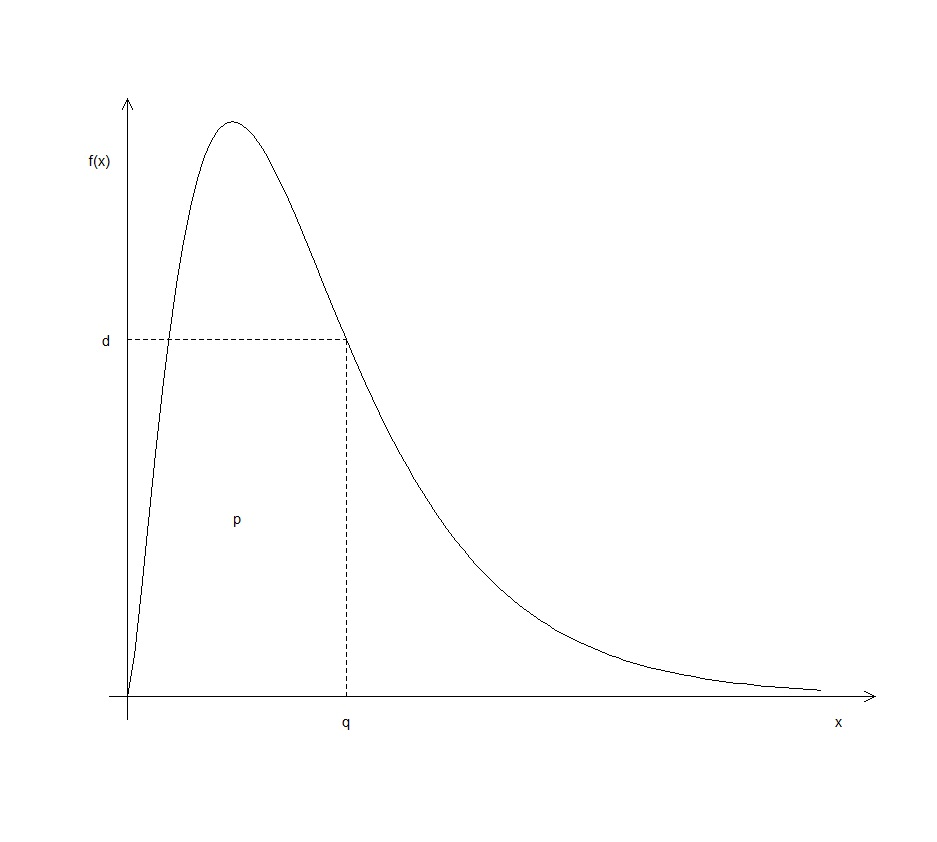
\includegraphics[width=1\linewidth]{pics/F-distribution} \caption{Meaning of the letters d, p and q when preceding an R distribution identifier.}\label{fig:Fdist}
\end{figure}

\subsection{Functions for categorical variables}\label{areagrp}

Apart from being \emph{{numeric}} or \emph{{logical}}, data in R can also be \emph{{categorical}} (\emph{{factor}} in R) or character strings. Study in detail the functions operating on factor data in Table \ref{tab:CatFunc}.

\begin{enumerate}
\def\labelenumi{(\alph{enumi})}
\item
  Use \texttt{cut()} to create an object \texttt{areagrp} to divide the \texttt{state.x77} data set into three groups representing the states with area within the intervals \((0, 10 000]\),\((10 000, 100 000]\) and \((100 000, Inf]\), respectively. \emph{Hint}: First study the arguments of \texttt{cut()}.
\item
  Repeat (a) with argument \texttt{labels\ =\ ??} to specify each state as being \emph{Small}, \emph{Medium} or \emph{Large} with respect to its area.
\item
  Use \texttt{unclass()} to obtain the numeric codes associated with each level of \texttt{areagrp}.
\item
  Repeat (a) to obtain \texttt{areagrp2} containing five equally spaced categories.
\item
  Repeat (a) to obtain \texttt{areagrp3} containing five groups with each containing \(20\%\) of the data.
\item
  Use \texttt{cut()} to create an object \texttt{illitgrp} to divide the \texttt{state.x77} data set into five groups representing the states with illiteracy within the interval \([0, 0.50)\), \([0.50, 1.00)\), \([1.00, 1.50)\), \([1.50, 2.00)\) and \([2.00, 5.00)\), respectively.
\item
  Obtain a two-way table of the \texttt{state.x77} data set according to \texttt{areagrp} and \texttt{illitgrp}.
\end{enumerate}

\begin{longtable}[]{@{}
  >{\raggedright\arraybackslash}p{(\linewidth - 2\tabcolsep) * \real{0.2857}}
  >{\raggedright\arraybackslash}p{(\linewidth - 2\tabcolsep) * \real{0.7143}}@{}}
\caption{\label{tab:CatFunc} Basic functions for categorical variables.}\tabularnewline
\toprule\noalign{}
\begin{minipage}[b]{\linewidth}\raggedright
\emph{{Function}}
\end{minipage} & \begin{minipage}[b]{\linewidth}\raggedright
\emph{{What it does}}
\end{minipage} \\
\midrule\noalign{}
\endfirsthead
\toprule\noalign{}
\begin{minipage}[b]{\linewidth}\raggedright
\emph{{Function}}
\end{minipage} & \begin{minipage}[b]{\linewidth}\raggedright
\emph{{What it does}}
\end{minipage} \\
\midrule\noalign{}
\endhead
\bottomrule\noalign{}
\endlastfoot
\texttt{cut()} & Creates categories out of a continuous variable \\
\texttt{factor()} & Encodes a vector as a \textbf{\emph{nominal}} categorical variable \\
\texttt{ordered()} & Encodes a vector as a \textbf{\emph{ordinal}} categorical variable when argument ordered is set to TRUE \\
\texttt{levels()} & Displays or sets the levels of a factor variable \\
\texttt{pretty()} & Creates convenient break points for a categorical variable \\
\texttt{split()} & Breaks up an array according to the value of a categorical variable \\
\texttt{table()} & Counts the number of observations cross-classified by categories \\
\texttt{unclass()} & Returns the numeric codes for representing the levels of a factor variable \\
\end{longtable}

\subsection{Functions for character manipulation}\label{character}

Study the functions in Table \ref{tab:CharFunc} in detail.

\begin{longtable}[]{@{}
  >{\raggedright\arraybackslash}p{(\linewidth - 2\tabcolsep) * \real{0.2857}}
  >{\raggedright\arraybackslash}p{(\linewidth - 2\tabcolsep) * \real{0.7143}}@{}}
\caption{\label{tab:CharFunc} Basic functions for character manipulation.}\tabularnewline
\toprule\noalign{}
\begin{minipage}[b]{\linewidth}\raggedright
\emph{{Function}}
\end{minipage} & \begin{minipage}[b]{\linewidth}\raggedright
\emph{{What it does}}
\end{minipage} \\
\midrule\noalign{}
\endfirsthead
\toprule\noalign{}
\begin{minipage}[b]{\linewidth}\raggedright
\emph{{Function}}
\end{minipage} & \begin{minipage}[b]{\linewidth}\raggedright
\emph{{What it does}}
\end{minipage} \\
\midrule\noalign{}
\endhead
\bottomrule\noalign{}
\endlastfoot
\texttt{abbreviate()} & Generates abbreviations of character values \\
\texttt{cat()} & Display,messages and/or values on screen or send to file \\
\texttt{grep()} & Search for patterns in characters \\
\texttt{nchar()} & Number of characters in a string \\
\texttt{paste()} & Combine values into character strings \\
\texttt{strsplit()} & Split the elements of a character vector \(\times\) into substrings \\
\texttt{substring()} & Extracts parts of character strings \\
\end{longtable}

\begin{enumerate}
\def\labelenumi{(\alph{enumi})}
\item
  What is the returned value of \texttt{grep\ ("ia",\ state.name)}?
\item
  Discuss the usage of \texttt{grep\ ("ia",\ state.name)}.
\item
  Discuss the output of \texttt{objects\ (pos\ =\ grep("stats",\ search()))}.
\item
  Use \texttt{paste()} to create variable names: var1, var2, \ldots, var100.
\item
  Repeat (d) to create variable names: var\_1, var\_2, \ldots, var\_100.
\item
  Discuss the output of:
\end{enumerate}

\begin{Shaded}
\begin{Highlighting}[]
\NormalTok{substring (paste (letters, collapse = ""),  }
\NormalTok{             1:nchar (paste (letters, collapse="")), }
\NormalTok{             1:nchar (paste (letters, collapse="")))}
\end{Highlighting}
\end{Shaded}

\begin{enumerate}
\def\labelenumi{(\alph{enumi})}
\setcounter{enumi}{6}
\tightlist
\item
  From the Help menu, select Manuals (in PDF) and open the Introduction to R document. Obtain a copy of the first two paragraphs of the Preface on page 1 of this book in the R commands window. Use this copy to calculate the number of words as well as the total number of characters (including spaces between words) in the passage.
\end{enumerate}

We are going to use several of the functions in Table \ref{tab:CharFunc} to perform this task in steps. Proceed as follows in R after copying the relevant passage to the clipboard:

\begin{Shaded}
\begin{Highlighting}[]
\NormalTok{TextPar }\OtherTok{\textless{}{-}} \FunctionTok{scan}\NormalTok{(}\AttributeTok{file =} \StringTok{"clipboard"}\NormalTok{, }\AttributeTok{what =} \StringTok{""}\NormalTok{)}
\end{Highlighting}
\end{Shaded}

To obtain a vector containing each of the words as a separate element.

\begin{Shaded}
\begin{Highlighting}[]
\NormalTok{TextPar }\OtherTok{\textless{}{-}} \FunctionTok{paste}\NormalTok{ (TextPar, }\AttributeTok{collapse =} \StringTok{" "}\NormalTok{)}
\end{Highlighting}
\end{Shaded}

To convert \texttt{TextPar} into a vector containing one element consisting of all the words concatenated and separated by spaces into a single character string. Add the correct line breaks (``\textbackslash n'') in \texttt{TextPar} using e.g.~\texttt{fix()}.

\begin{Shaded}
\begin{Highlighting}[]
\NormalTok{TextPar }\OtherTok{\textless{}{-}} \FunctionTok{strsplit}\NormalTok{(}\AttributeTok{x =}\NormalTok{ TextPar, }\AttributeTok{split =} \StringTok{\textquotesingle{}}\SpecialCharTok{\textbackslash{}n}\StringTok{\textquotesingle{}}\NormalTok{)}
\end{Highlighting}
\end{Shaded}

\begin{Shaded}
\begin{Highlighting}[]
\NormalTok{mode(TextPar)}
\NormalTok{[1] "list"}

\NormalTok{mode(unlist(TextPar))}
\NormalTok{[1] "character" }
\end{Highlighting}
\end{Shaded}

\begin{Shaded}
\begin{Highlighting}[]
\NormalTok{TextPar }\OtherTok{\textless{}{-}} \FunctionTok{unlist}\NormalTok{(TextPar)}
\end{Highlighting}
\end{Shaded}

To change \texttt{TextPar} into a character vector.

\begin{Shaded}
\begin{Highlighting}[]
\FunctionTok{nchar}\NormalTok{(TextPar)}
\FunctionTok{length}\NormalTok{(TextPar)}
\end{Highlighting}
\end{Shaded}

\section{Differentiation and integration}\label{differentiation-and-integration}

\subsection{Symbolic differentiation}\label{symbolic-differentiation}

Study the help files of \texttt{D()} and \texttt{deriv()}.

\subsection{Integration}\label{integration}

Study the help file of \texttt{integrate()}.

\subsection{Exercise}\label{exercise-8}

\begin{enumerate}
\def\labelenumi{(\arabic{enumi})}
\item
  It is known from elementary statistics that approximately 68\% of data from a normal distribution with a mean of zero and a standard deviation of unity will have an absolute value less than unity. Use the \texttt{sum()} and \texttt{rnorm()} functions to find the proportion of \(n\) random \(normal (0, 1)\) variables whose absolute value is less than \(1.0\). Repeat with different values for \(n\) to investigate how widely the results vary.
\item
  Define: conditional inverse and generalized (Moore-Penrose) inverse for matrix \(\mathbf{X}: p \times q\) and make provision for \(p = q\), \(p > q\) and \(p < q\). First, show how the svd of \(\mathbf{X}\) can be used to obtain a conditional inverse, \(\mathbf{X}^c\) for \(\mathbf{X}\). Now use the above information to write an R function for calculating \(\mathbf{X}^c\) for any given \(\mathbf{X}\). The function must provide a test to check if the calculated conditional inverse is indeed a conditional inverse. Illustrate the usage of your function.
\item
  Give the necessary instructions to:

  \begin{enumerate}
  \def\labelenumii{(\roman{enumii})}
  \tightlist
  \item
    read into R an external text data file consisting of \(10\) sample observations with each consisting of one character variable and two numerical variables.
  \item
    read into R a large external text data file consisting of \(50\) numerical variables but unknown number of records. Each record in this data file takes up 5 lines. The variables in the R object must have the names X1, \ldots, X50.
  \end{enumerate}
\item
  Discuss the meaning of the following R instructions:

  \begin{enumerate}
  \def\labelenumii{(\roman{enumii})}
  \tightlist
  \item
    \texttt{y\ \textless{}-\ x{[}!is.na(x){]}}
  \item
    \texttt{z\ \textless{}-\ (x\ +\ y){[}!is.na(x)\ \&\ x\ \textgreater{}0{]}}
  \item
    \texttt{a\ \textless{}-\ x{[}-(1:5){]}}
  \item
    \texttt{x{[}is.na(x){]}\ \textless{}-\ 0}
  \end{enumerate}
\end{enumerate}

\chapter{Introducing traditional R graphics}\label{graphics}

A basic knowledge of R graphics is needed before directing attention to the art of writing programs (functions) in R. Therefore, in this chapter a brief overview is given of the basics of traditional R graphics. In a later chapter, after studying the principles of R programming, a second round of R graphics will follow.

\section{General}\label{general-1}

Study the graphical parameters by requesting

\begin{Shaded}
\begin{Highlighting}[]
\NormalTok{?par}
\end{Highlighting}
\end{Shaded}

In Figure \ref{fig:figRegion} the main components of a graph window are illustrated. Study this figure in detail. The \emph{{Plot Region}} together with the \emph{{Margins}} is called the \emph{{Figure Region}}.

\begin{figure}
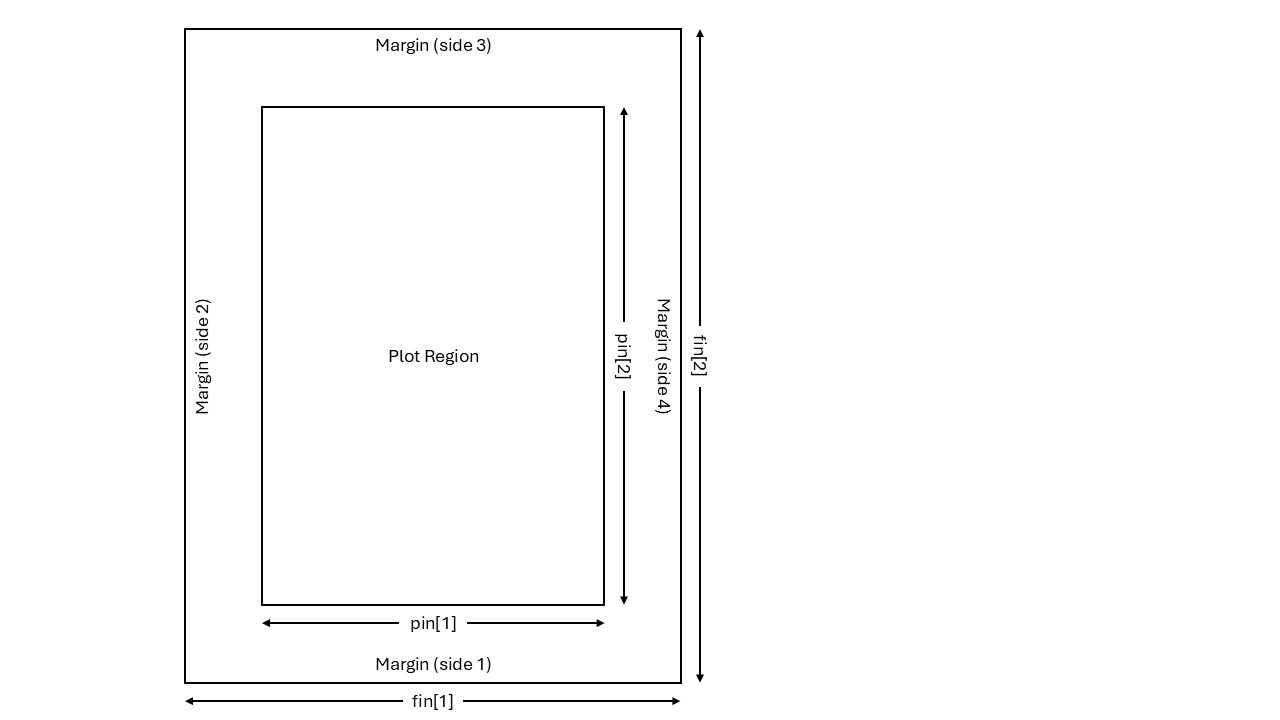
\includegraphics[width=1\linewidth]{pics/figMargins} \caption{The main components of a graph window and the parameters for controlling their sizes.  The parameter mai is a numerical vector of the form c(bottom, left, top, right) specifying the margins in inches while the parameter mar has a similar form specifying the respective margins as the number of lines. The default of mar is c(5, 4, 4, 2) + 0.1.}\label{fig:figRegion}
\end{figure}

\begin{enumerate}
\def\labelenumi{(\alph{enumi})}
\item
  What is the difference between high-level and low-level plotting instructions?
\item
  Take note especially how the functions \texttt{windows()}, \texttt{win.graph()} or \texttt{x11()} are used as well as the different options available for these functions.
\item
  The instruction \texttt{dev.new()} allows opening a new graph window in a platform-independent way.
\item
  In this chapter some high-level plotting instructions are studied. Each of these instructions results in a (new) graph window with a complete graph drawn. The command \texttt{graphics.off()} deletes all open graphic devices.
\item
  Study the use of \texttt{par()}, \texttt{par(mfrow\ =)} and \texttt{par(mfcol\ =)}. Study the use of \texttt{par(new\ =\ TRUE)} to plot more than one figure on the same set of axes.
\item
  Study how the functions \texttt{graphics.off()} and \texttt{dev.off()} work.
\end{enumerate}

\section{High-level plotting instructions}\label{highLevelPlotting}

\begin{enumerate}
\def\labelenumi{(\alph{enumi})}
\tightlist
\item
  Construct a barplot of the illiteracy of the states according to the \texttt{areagrp} (as defined in section \ref{areagrp}) in the \texttt{state.x77} dataframe. \emph{Hint}: The function \texttt{tapply()} operates on a vector given as its first argument. Its second argument groups the first argument into groups so that the function given in its third argument can be applied to each of these groups. Study the following command:
\end{enumerate}

\begin{Shaded}
\begin{Highlighting}[]
\FunctionTok{barplot}\NormalTok{ (}\FunctionTok{tapply}\NormalTok{ (state.x77[, }\StringTok{"Illiteracy"}\NormalTok{], areagrp, mean), }
         \AttributeTok{names=}\FunctionTok{levels}\NormalTok{(areagrp), }\AttributeTok{ylab =} \StringTok{"Illiteracy"}\NormalTok{, }\AttributeTok{xlab =} \StringTok{"Area of State"}\NormalTok{, }
         \AttributeTok{main =} \StringTok{"Barplot of Mean Illiteracy"}\NormalTok{)}
\end{Highlighting}
\end{Shaded}

\begin{enumerate}
\def\labelenumi{(\alph{enumi})}
\setcounter{enumi}{1}
\tightlist
\item
  Construct, for the \texttt{state.x77} data set, box plots of illiteracy broken down by the income of the states. First use \texttt{cut()} to form three categories of state income:
\end{enumerate}

\begin{Shaded}
\begin{Highlighting}[]
\NormalTok{state.income }\OtherTok{\textless{}{-}} \FunctionTok{cut}\NormalTok{ (state.x77[ , }\StringTok{"Income"}\NormalTok{], }\FunctionTok{c}\NormalTok{(}\DecValTok{0}\NormalTok{, }\DecValTok{4000}\NormalTok{, }\DecValTok{5000}\NormalTok{, }\ConstantTok{Inf}\NormalTok{),}
                   \AttributeTok{labels=}\FunctionTok{c}\NormalTok{(}\StringTok{"$4000 or less"}\NormalTok{, }\StringTok{"$4001{-}$5000"}\NormalTok{, }\StringTok{"more than $5001"}\NormalTok{))}
\end{Highlighting}
\end{Shaded}

Then use \texttt{boxplot()} together with \texttt{split()} to produce the desired graph:

\begin{Shaded}
\begin{Highlighting}[]
\FunctionTok{boxplot}\NormalTok{ (}\FunctionTok{split}\NormalTok{ (state.x77[ , }\StringTok{"Income"}\NormalTok{], state.income))}
\end{Highlighting}
\end{Shaded}

Add labels for the axes as well as a title for the figure.

\begin{enumerate}
\def\labelenumi{(\alph{enumi})}
\setcounter{enumi}{2}
\item
  Repeat the previous example but use argument \texttt{notch\ =\ TRUE}.
\item
  Attach the package \texttt{akima}. What is the usage of the function \texttt{interp()}? Discuss by constructing the following contour plot:
\end{enumerate}

\begin{Shaded}
\begin{Highlighting}[]
\FunctionTok{contour}\NormalTok{ (}\FunctionTok{interp}\NormalTok{ (state.center}\SpecialCharTok{$}\NormalTok{x, state.center}\SpecialCharTok{$}\NormalTok{y,  state.x77[,}\StringTok{"Frost"}\NormalTok{])) }
\end{Highlighting}
\end{Shaded}

\begin{enumerate}
\def\labelenumi{(\alph{enumi})}
\setcounter{enumi}{4}
\tightlist
\item
  What is a \emph{{coplot}}? Discuss after giving the following instruction and referring to the role of the tilde (\textasciitilde) operator.
\end{enumerate}

\begin{Shaded}
\begin{Highlighting}[]
\FunctionTok{coplot}\NormalTok{ (state.x77[,}\StringTok{"Illiteracy"}\NormalTok{] }\SpecialCharTok{\textasciitilde{}}\NormalTok{ state.x77[,}\StringTok{"Area"}\NormalTok{] }\SpecialCharTok{|}\NormalTok{ state.x77[,}\StringTok{"Income"}\NormalTok{])}
\end{Highlighting}
\end{Shaded}

\begin{enumerate}
\def\labelenumi{(\alph{enumi})}
\setcounter{enumi}{5}
\tightlist
\item
  A \emph{{dotchart}} is constructed with function \texttt{dotchart()}. First some preparations are necessary:
\end{enumerate}

\begin{Shaded}
\begin{Highlighting}[]
\NormalTok{incgroup }\OtherTok{\textless{}{-}} \FunctionTok{cut}\NormalTok{(state.x77[,}\StringTok{"Income"}\NormalTok{],  }\DecValTok{3}\NormalTok{, }
                \AttributeTok{labels =} \FunctionTok{c}\NormalTok{(}\StringTok{"LowInc"}\NormalTok{, }\StringTok{"MediumInc"}\NormalTok{, }\StringTok{"HighInc"}\NormalTok{))}
\NormalTok{lifgroup }\OtherTok{\textless{}{-}} \FunctionTok{cut}\NormalTok{(state.x77[,}\StringTok{"Life Exp"}\NormalTok{], }\DecValTok{2}\NormalTok{, }
                \AttributeTok{labels =} \FunctionTok{c}\NormalTok{(}\StringTok{"LowExp"}\NormalTok{, }\StringTok{"HighExp"}\NormalTok{))}
\NormalTok{table.out }\OtherTok{\textless{}{-}} \FunctionTok{tapply}\NormalTok{(state.x77 [,}\StringTok{"Income"}\NormalTok{], }\FunctionTok{list}\NormalTok{(lifgroup,incgroup), mean)}
\NormalTok{table.out}
\CommentTok{\#\textgreater{}           LowInc MediumInc HighInc}
\CommentTok{\#\textgreater{} LowExp  3640.917  4698.417    5807}
\CommentTok{\#\textgreater{} HighExp 4039.600  4697.667    5348}
\FunctionTok{dotchart}\NormalTok{ (table.out, }
          \FunctionTok{levels}\NormalTok{ (}\FunctionTok{factor}\NormalTok{ (}\FunctionTok{col}\NormalTok{ (table.out), }
                          \AttributeTok{labels =} \FunctionTok{levels}\NormalTok{ (incgroup)))[}\FunctionTok{col}\NormalTok{(table.out)], }
          \FunctionTok{factor}\NormalTok{(}\FunctionTok{row}\NormalTok{(table.out), }\AttributeTok{labels =} \FunctionTok{levels}\NormalTok{(lifgroup)))}
\end{Highlighting}
\end{Shaded}

\pandocbounded{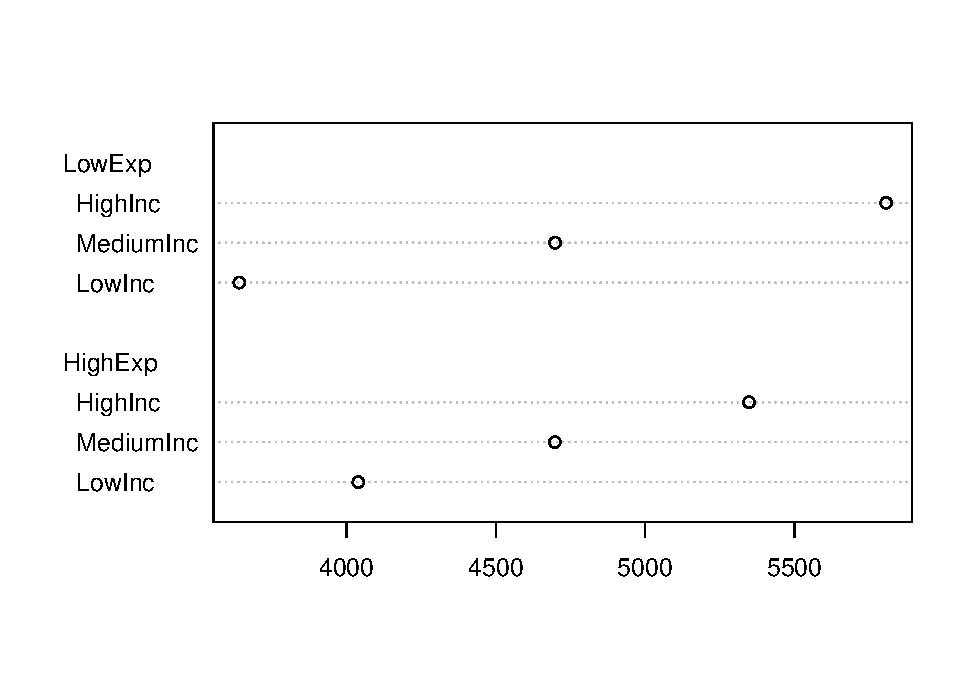
\includegraphics[keepaspectratio]{04-graphics_files/figure-latex/dotchart-1.pdf}}

Complete the graph by adding a label to the x-axis and a heading for the graph.

\begin{enumerate}
\def\labelenumi{(\alph{enumi})}
\setcounter{enumi}{6}
\item
  Use function \texttt{faces()} available in package \texttt{aplpack} to construct Chernoff faces for the Western states in the data set \texttt{state.x77}. \emph{Hint}: The Western states appear in rows 3, 5, 12, 26, 28, 37, 44, 47 and 50. Explain what is represented by each of the facial features. First set argument \texttt{face.type\ =\ 0} and then \texttt{face.type\ =\ 1}.
\item
  Obtain a histogram of the life expectancy in the states of \texttt{state.x77}.
\item
  Execute the command
\end{enumerate}

\begin{Shaded}
\begin{Highlighting}[]
\FunctionTok{pairs}\NormalTok{ (state.x77)}
\end{Highlighting}
\end{Shaded}

Interpret the graph.

\begin{enumerate}
\def\labelenumi{(\alph{enumi})}
\setcounter{enumi}{9}
\tightlist
\item
  Three-dimensional graphs are constructed with function \texttt{persp()}.
\end{enumerate}

\begin{Shaded}
\begin{Highlighting}[]
\NormalTok{pts }\OtherTok{\textless{}{-}} \FunctionTok{seq}\NormalTok{(}\AttributeTok{from =} \SpecialCharTok{{-}}\NormalTok{pi, }\AttributeTok{to =}\NormalTok{ pi, }\AttributeTok{len =} \DecValTok{20}\NormalTok{)}
\NormalTok{z }\OtherTok{\textless{}{-}} \FunctionTok{outer}\NormalTok{(}\AttributeTok{X =}\NormalTok{ pts, }\AttributeTok{Y =}\NormalTok{ pts, }\ControlFlowTok{function}\NormalTok{(x,y) }\FunctionTok{sin}\NormalTok{(x)}\SpecialCharTok{*}\FunctionTok{cos}\NormalTok{(y))}
\FunctionTok{persp}\NormalTok{(}\AttributeTok{x =}\NormalTok{ pts, }\AttributeTok{y =}\NormalTok{ pts, z, }\AttributeTok{theta =} \DecValTok{10}\NormalTok{, }\AttributeTok{phi =} \DecValTok{60}\NormalTok{, }\AttributeTok{ticktype =} \StringTok{\textquotesingle{}detailed\textquotesingle{}}\NormalTok{)}
\end{Highlighting}
\end{Shaded}

Discuss the meaning of each of the above instructions. Experiment with different values for arguments \texttt{theta} and \texttt{phi}.

\begin{enumerate}
\def\labelenumi{(\alph{enumi})}
\setcounter{enumi}{10}
\item
  Obtain a pie chart of the object \texttt{areagrp} defined in section \ref{areagrp}. \emph{Hint}: function \texttt{table()} may be useful here.
\item
  A cluster plot (dendrogram) can be constructed with function \texttt{plclust()} as follows:
\end{enumerate}

\begin{Shaded}
\begin{Highlighting}[]
\NormalTok{west.rows }\OtherTok{\textless{}{-}} \FunctionTok{c}\NormalTok{(}\DecValTok{3}\NormalTok{, }\DecValTok{5}\NormalTok{, }\DecValTok{12}\NormalTok{, }\DecValTok{26}\NormalTok{, }\DecValTok{28}\NormalTok{, }\DecValTok{37}\NormalTok{, }\DecValTok{44}\NormalTok{, }\DecValTok{47}\NormalTok{, }\DecValTok{50}\NormalTok{)}
\NormalTok{distmat.west }\OtherTok{\textless{}{-}} \FunctionTok{dist}\NormalTok{ (}\FunctionTok{scale}\NormalTok{ (state.x77[west.rows,]))}
\FunctionTok{plot}\NormalTok{(}\FunctionTok{hclust}\NormalTok{(distmat.west), }\AttributeTok{labels =} \FunctionTok{rownames}\NormalTok{(state.x77)[west.rows])}
\end{Highlighting}
\end{Shaded}

Interpret the above instructions and the resulting plot.

\begin{enumerate}
\def\labelenumi{(\alph{enumi})}
\setcounter{enumi}{12}
\item
  Use the function \texttt{plot()} to plot \(sin (\theta)\) as \(\theta\) varies from \(–\pi\) to \(\pi\).
\item
  Could you explain the different graphs resulting from the two calls in (l) and (m) to the \texttt{plot()} function above?
\item
  Obtain the empirical distribution function of variable \texttt{Life\ Exp} in the \texttt{state.x77} data set by using the functions \texttt{cut()}, \texttt{ecdf()} and \texttt{plot()}.
\item
  Check the normality of variable \texttt{Income} in the \texttt{state.x7}7 data set by using function \texttt{qqnorm()}.
\item
  Obtain a \texttt{qqplot} of the income of small states versus the income of large states in the data set \texttt{state.x77} where small and large are defined as below or above the median income, respectively.
\end{enumerate}

\begin{Shaded}
\begin{Highlighting}[]
\NormalTok{state.size }\OtherTok{\textless{}{-}} \FunctionTok{cut}\NormalTok{ (state.x77[,}\StringTok{"Area"}\NormalTok{],  }
                   \FunctionTok{c}\NormalTok{(}\DecValTok{0}\NormalTok{, }\FunctionTok{median}\NormalTok{ (state.x77[,}\StringTok{"Area"}\NormalTok{]), }\FunctionTok{max}\NormalTok{ (state.x77[,}\StringTok{"Area"}\NormalTok{])))}
\NormalTok{state.income }\OtherTok{\textless{}{-}} \FunctionTok{split}\NormalTok{ (state.x77[,}\StringTok{"Income"}\NormalTok{], state.size)}
\FunctionTok{qqplot}\NormalTok{(state.income[[}\DecValTok{1}\NormalTok{]], state.income[[}\DecValTok{2}\NormalTok{]], }\AttributeTok{xlab=}\StringTok{"Income for small states"}\NormalTok{, }
       \AttributeTok{ylab=}\StringTok{"income for large states"}\NormalTok{)}
\end{Highlighting}
\end{Shaded}

\begin{enumerate}
\def\labelenumi{(\alph{enumi})}
\setcounter{enumi}{17}
\tightlist
\item
  Use function \texttt{ts.plot()} to construct a time series plot of the sunspots data set.
\end{enumerate}

\section{Interactive communication with graphs}\label{interactive-communication-with-graphs}

\begin{enumerate}
\def\labelenumi{(\alph{enumi})}
\item
  Study the help files of the functions \texttt{text()}, \texttt{identify()} and \texttt{locator()}.
\item
  Illustrate the usage of \texttt{identify()} on a scatterplot of variables \texttt{Illiteracy} and \texttt{Life\ Exp} in the \texttt{state.x77} data set:
\end{enumerate}

\begin{Shaded}
\begin{Highlighting}[]
\FunctionTok{plot}\NormalTok{ (}\AttributeTok{x =}\NormalTok{ state.x77[,}\StringTok{\textquotesingle{}Life Exp\textquotesingle{}}\NormalTok{], }\AttributeTok{y =}\NormalTok{ state.x77[,}\StringTok{\textquotesingle{}Income\textquotesingle{}}\NormalTok{])}
\end{Highlighting}
\end{Shaded}

To create the scatterplot, then call

\begin{Shaded}
\begin{Highlighting}[]
\FunctionTok{identify}\NormalTok{ (}\AttributeTok{x =}\NormalTok{ state.x77[,}\StringTok{\textquotesingle{}Life Exp\textquotesingle{}}\NormalTok{], }\AttributeTok{y =}\NormalTok{ state.x77[,}\StringTok{\textquotesingle{}Income\textquotesingle{}}\NormalTok{], }
          \FunctionTok{seq}\NormalTok{ (}\AttributeTok{along =} \FunctionTok{rownames}\NormalTok{(state.x77)), }\AttributeTok{n =} \DecValTok{5}\NormalTok{)}
\end{Highlighting}
\end{Shaded}

Notice the change in the cursor; the cursor changes to a cross when moved over the graph. Hover the cursor over a point to identify and click left mouse button. Repeat \(n = 5\) times. Explain the result. Next, create the scatterplot once more and then call

\begin{Shaded}
\begin{Highlighting}[]
\FunctionTok{identify}\NormalTok{ (}\AttributeTok{x =}\NormalTok{ state.x77[,}\StringTok{\textquotesingle{}Life Exp\textquotesingle{}}\NormalTok{],  }\AttributeTok{y =}\NormalTok{ state.x77[,}\StringTok{\textquotesingle{}Income\textquotesingle{}}\NormalTok{], }
          \AttributeTok{labels =} \FunctionTok{rownames}\NormalTok{(state.x77)[}\FunctionTok{seq}\NormalTok{ (}\AttributeTok{along =} 
                                              \FunctionTok{rownames}\NormalTok{(state.x77))] , }\AttributeTok{n =} \DecValTok{5}\NormalTok{) }
\end{Highlighting}
\end{Shaded}

Explain what has happened.

\begin{enumerate}
\def\labelenumi{(\alph{enumi})}
\setcounter{enumi}{2}
\tightlist
\item
  Illustrate the usage of \texttt{locator()} by:
\end{enumerate}

\begin{enumerate}
\def\labelenumi{(\roman{enumi})}
\tightlist
\item
  Joining \(5\) user defined points on a graph interactively with straight lines.
\end{enumerate}

\begin{Shaded}
\begin{Highlighting}[]
\FunctionTok{plot}\NormalTok{ (}\AttributeTok{x =}\NormalTok{ state.x77[,}\StringTok{\textquotesingle{}Life Exp\textquotesingle{}}\NormalTok{], }\AttributeTok{y =}\NormalTok{ state.x77[,}\StringTok{\textquotesingle{}Income\textquotesingle{}}\NormalTok{])}
\FunctionTok{locator}\NormalTok{(}\DecValTok{5}\NormalTok{, }\AttributeTok{type =} \StringTok{"l"}\NormalTok{) }
\end{Highlighting}
\end{Shaded}

Use mouse and select the five points on the graph. What happened on the graph? What happened in the commands window?

\begin{enumerate}
\def\labelenumi{(\roman{enumi})}
\setcounter{enumi}{1}
\tightlist
\item
  Writing text interactively at a specified position on an existing graph.
\end{enumerate}

\begin{Shaded}
\begin{Highlighting}[]
\FunctionTok{plot}\NormalTok{ (}\AttributeTok{x =}\NormalTok{ state.x77[,}\StringTok{\textquotesingle{}Life Exp\textquotesingle{}}\NormalTok{], }\AttributeTok{y =}\NormalTok{ state.x77[,}\StringTok{\textquotesingle{}Income\textquotesingle{}}\NormalTok{])}
\FunctionTok{text}\NormalTok{ (}\FunctionTok{locator}\NormalTok{ (}\AttributeTok{n =} \DecValTok{1}\NormalTok{, }\AttributeTok{type =} \StringTok{"n"}\NormalTok{), }\AttributeTok{label =} \StringTok{"State with the highest income"}\NormalTok{)}
\end{Highlighting}
\end{Shaded}

\section{3D graphics: package rgl}\label{d-graphics-package-rgl}

Write and execute the following function.

\begin{Shaded}
\begin{Highlighting}[]
\NormalTok{rgl.example }\OtherTok{\textless{}{-}} \ControlFlowTok{function}\NormalTok{ (}\AttributeTok{size =} \FloatTok{0.1}\NormalTok{, }\AttributeTok{col =} \StringTok{"green"}\NormalTok{, }\AttributeTok{alpha.3d =} \FloatTok{0.6}\NormalTok{) }
\NormalTok{\{ }\FunctionTok{require}\NormalTok{(rgl)}
\NormalTok{  datmat }\OtherTok{\textless{}{-}} \FunctionTok{matrix}\NormalTok{ (}\FunctionTok{rnorm}\NormalTok{ (}\DecValTok{30}\NormalTok{), }\AttributeTok{ncol =} \DecValTok{3}\NormalTok{)}
  \FunctionTok{open3d}\NormalTok{()}
  \FunctionTok{spheres3d}\NormalTok{ (datmat,}\AttributeTok{radius =}\NormalTok{ size, }\AttributeTok{color =}\NormalTok{ col, }\AttributeTok{alpha =}\NormalTok{ alpha}\FloatTok{.3}\NormalTok{d)}
  \FunctionTok{axes3d}\NormalTok{(}\AttributeTok{col =} \StringTok{"black"}\NormalTok{)}
\NormalTok{  device.ID }\OtherTok{\textless{}{-}} \FunctionTok{rgl.cur}\NormalTok{()}
\NormalTok{  answer }\OtherTok{\textless{}{-}} \FunctionTok{readline}\NormalTok{ (}\StringTok{"Save 3D graph as a .png file? Y/N}\SpecialCharTok{\textbackslash{}n}\StringTok{"}\NormalTok{)}
  \ControlFlowTok{while}\NormalTok{ (}\SpecialCharTok{!}\NormalTok{(answer }\SpecialCharTok{==} \StringTok{"Y"} \SpecialCharTok{|}\NormalTok{ answer }\SpecialCharTok{==} \StringTok{"y"} \SpecialCharTok{|}\NormalTok{ answer }\SpecialCharTok{==} \StringTok{"N"} \SpecialCharTok{|}\NormalTok{ answer }\SpecialCharTok{==} \StringTok{"n"}\NormalTok{)) }
\NormalTok{    answer }\OtherTok{\textless{}{-}} \FunctionTok{readline}\NormalTok{(}\StringTok{"Save 3D graph as a .png file? Y/N}\SpecialCharTok{\textbackslash{}n}\StringTok{"}\NormalTok{)}
  \ControlFlowTok{if}\NormalTok{ (answer }\SpecialCharTok{==} \StringTok{"Y"} \SpecialCharTok{|}\NormalTok{ answer }\SpecialCharTok{==} \StringTok{"y"}\NormalTok{) }
    \ControlFlowTok{repeat} 
\NormalTok{    \{ file.name }\OtherTok{\textless{}{-}} \FunctionTok{readline}\NormalTok{ (}\StringTok{"Provide file name including full }
\StringTok{                              path NOT in quotes and SINGLE }
\StringTok{                              back slashes!}\SpecialCharTok{\textbackslash{}n}\StringTok{"}\NormalTok{)}
\NormalTok{      file.name }\OtherTok{\textless{}{-}} \FunctionTok{paste}\NormalTok{ (file.name, }\StringTok{".png"}\NormalTok{, }\AttributeTok{sep =} \StringTok{""}\NormalTok{)}
      \FunctionTok{snapshot3d}\NormalTok{ (}\AttributeTok{file =}\NormalTok{ file.name)}
      \FunctionTok{rgl.set}\NormalTok{ (device.ID)}
\NormalTok{      answer2 }\OtherTok{\textless{}{-}} \FunctionTok{readline}\NormalTok{(}\StringTok{"Save another 3D graph as a .png file? Y/N }\SpecialCharTok{\textbackslash{}n}\StringTok{"}\NormalTok{)}
      \ControlFlowTok{if}\NormalTok{ (answer2 }\SpecialCharTok{==} \StringTok{"Y"} \SpecialCharTok{|}\NormalTok{ answer2 }\SpecialCharTok{==} \StringTok{"y"}\NormalTok{) }\ControlFlowTok{next} \ControlFlowTok{else} \ControlFlowTok{break}
\NormalTok{    \}}
  \ControlFlowTok{else} \FunctionTok{rgl.set}\NormalTok{ (device.ID)}
\NormalTok{\}}
\end{Highlighting}
\end{Shaded}

Study the above code and constructions in detail.

\section{Exercise}\label{exercise-9}

\begin{enumerate}
\def\labelenumi{\arabic{enumi}.}
\item
  Obtain a graph of a \(normal(100, 25)\) probability density function (p.d.f.).
\item
  Plot on the same set of axes

  \begin{enumerate}
  \def\labelenumii{(\roman{enumii})}
  \tightlist
  \item
    a central \(beta(9, 5)\) p.d.f.;
  \item
    a non-central \(beta(9 5)\) p.d.f. with non-centrality parameter = \(15\) and
  \item
    a non-central \(beta(9, 5)\) p.d.f. with non-centrality parameter = \(40\).
  \end{enumerate}
\end{enumerate}

Add a suitable legend to the plot.

\begin{enumerate}
\def\labelenumi{\arabic{enumi}.}
\setcounter{enumi}{2}
\tightlist
\item
  Use \texttt{persp()} to obtain a graph of any user specified bivariate function. The challenge is that the function specification must appear as the main title of the graph. In order to address this problem we need information about the arguments of \texttt{persp()}:
\end{enumerate}

\begin{Shaded}
\begin{Highlighting}[]
\FunctionTok{args}\NormalTok{ (persp)}
\CommentTok{\#\textgreater{} function (x, ...) }
\CommentTok{\#\textgreater{} NULL}
\end{Highlighting}
\end{Shaded}

This is not very helpful so we try

\begin{Shaded}
\begin{Highlighting}[]
\FunctionTok{methods}\NormalTok{ (persp)}
\CommentTok{\#\textgreater{} [1] persp.default*}
\CommentTok{\#\textgreater{} see \textquotesingle{}?methods\textquotesingle{} for accessing help and source code}
\FunctionTok{args}\NormalTok{ (persp.default)}
\CommentTok{\#\textgreater{} Error: object \textquotesingle{}persp.default\textquotesingle{} not found}
\end{Highlighting}
\end{Shaded}

The reason for this error message follows from the above as that \texttt{persp.default} is not visible. The immediate visibility of a function is regulated by a package builder through the package's namespace mechanism. Only object names that are exported are immediately visible; object names that are not exported are marked with an asterisk and are not visible. The functions
\texttt{argsAnywhere()} and \texttt{getAnywhere()} are available to get information on asterisked object names:

\begin{Shaded}
\begin{Highlighting}[]
\FunctionTok{argsAnywhere}\NormalTok{ (persp.default)}
\CommentTok{\#\textgreater{} function (x = seq(0, 1, length.out = nrow(z)), y = seq(0, 1, }
\CommentTok{\#\textgreater{}     length.out = ncol(z)), z, xlim = range(x), ylim = range(y), }
\CommentTok{\#\textgreater{}     zlim = range(z, na.rm = TRUE), xlab = NULL, ylab = NULL, }
\CommentTok{\#\textgreater{}     zlab = NULL, main = NULL, sub = NULL, theta = 0, phi = 15, }
\CommentTok{\#\textgreater{}     r = sqrt(3), d = 1, scale = TRUE, expand = 1, col = "white", }
\CommentTok{\#\textgreater{}     border = NULL, ltheta = {-}135, lphi = 0, shade = NA, box = TRUE, }
\CommentTok{\#\textgreater{}     axes = TRUE, nticks = 5, ticktype = "simple", ...) }
\CommentTok{\#\textgreater{} NULL}
\end{Highlighting}
\end{Shaded}

We notice that we can make use of the argument main in a call to \texttt{persp()} to provide our perspective plot with a title. However, main accepts only character strings and not mathematical expressions. Furthermore, we have seen in the \texttt{persp()} example in section \ref{highLevelPlotting} that the values for the argument \texttt{z} are conveniently found by a call to \texttt{outer()} using its argument \texttt{FUN}. However \texttt{FUN} requires a function. So we need the means to convert expressions into character strings and vice versa to convert character strings into expressions.

The following pairs of functions allow these conversions to be made:

Character strings ('' ``) → expressions: \texttt{parse()} and \texttt{eval()}

Expressions (unquoted) → character strings ('' ``): \texttt{deparse()} and \texttt{substitute()}

\begin{Shaded}
\begin{Highlighting}[]
\NormalTok{pts }\OtherTok{\textless{}{-}} \FunctionTok{seq}\NormalTok{ (}\AttributeTok{from =} \SpecialCharTok{{-}}\DecValTok{3}\NormalTok{, }\AttributeTok{to =} \DecValTok{3}\NormalTok{, }\AttributeTok{len =} \DecValTok{50}\NormalTok{)}
\NormalTok{fun1 }\OtherTok{\textless{}{-}} \StringTok{"2 * pi * exp({-}(x\^{}2 + y\^{}2)/2)"}
\NormalTok{fun2 }\OtherTok{\textless{}{-}} \FunctionTok{parse}\NormalTok{ (}\AttributeTok{text =} \FunctionTok{paste}\NormalTok{ (}\StringTok{"function(x,y)"}\NormalTok{, fun1))}
\end{Highlighting}
\end{Shaded}

Explain carefully what \texttt{parse()} is doing.

\begin{Shaded}
\begin{Highlighting}[]
\NormalTok{zz }\OtherTok{\textless{}{-}} \FunctionTok{outer}\NormalTok{ (pts, pts, }\FunctionTok{eval}\NormalTok{(fun2))}
\end{Highlighting}
\end{Shaded}

Explain carefully what \texttt{eval()} is doing.

\begin{Shaded}
\begin{Highlighting}[]
\FunctionTok{persp}\NormalTok{ (}\AttributeTok{x =}\NormalTok{ pts, }\AttributeTok{y =}\NormalTok{ pts, }\AttributeTok{z =}\NormalTok{ zz, }\AttributeTok{theta =} \DecValTok{0}\NormalTok{, }\AttributeTok{phi =} \DecValTok{15}\NormalTok{, }\AttributeTok{ticktype =} \StringTok{"detailed"}\NormalTok{, }
       \AttributeTok{main =} \FunctionTok{paste}\NormalTok{(}\StringTok{"Persp plot of \textasciigrave{}"}\NormalTok{fun2,}\StringTok{"\textasciigrave{}"}\NormalTok{,}\AttributeTok{sep=}\StringTok{""}\NormalTok{))}
\end{Highlighting}
\end{Shaded}

Explain carefully the role of \texttt{paste()}.

\begin{enumerate}
\def\labelenumi{\arabic{enumi}.}
\setcounter{enumi}{3}
\item
  Use the \texttt{volcano} data to:

  \begin{enumerate}
  \def\labelenumii{(\roman{enumii})}
  \item
    Obtain a perspective plot using \texttt{persp()}.
  \item
    Obtain an RGL plot of the \texttt{volcano} data.
  \end{enumerate}
\end{enumerate}

\chapter{Subscripting}\label{subscripting}

Vectorized arithmetic and subscripting are two cornerstones of R programming. Review section \ref{highLevelPlotting} for several examples where subscripting has been used. In this chapter subscripting is studied in detail. Specifically, the following two related topics are studied:

\begin{itemize}
\tightlist
\item
  Extracting parts of an object by using \emph{{subscripting}}.
\item
  The combination and rearranging of data within data structures like matrices, dataframes and lists.
\end{itemize}

\section{Subscripting with vectors}\label{vectorSubscripting}

The different types of subscripting with vectors are summarized in Table \ref{tab:SubscriptVectorTypes}:

\begin{longtable}[]{@{}
  >{\raggedright\arraybackslash}p{(\linewidth - 4\tabcolsep) * \real{0.1622}}
  >{\raggedright\arraybackslash}p{(\linewidth - 4\tabcolsep) * \real{0.5405}}
  >{\raggedright\arraybackslash}p{(\linewidth - 4\tabcolsep) * \real{0.2973}}@{}}
\caption{\label{tab:SubscriptVectorTypes} Different types of subscripting vectors.}\tabularnewline
\toprule\noalign{}
\begin{minipage}[b]{\linewidth}\raggedright
\emph{{Type}}
\end{minipage} & \begin{minipage}[b]{\linewidth}\raggedright
\emph{{Effect}}
\end{minipage} & \begin{minipage}[b]{\linewidth}\raggedright
\emph{{Example}}
\end{minipage} \\
\midrule\noalign{}
\endfirsthead
\toprule\noalign{}
\begin{minipage}[b]{\linewidth}\raggedright
\emph{{Type}}
\end{minipage} & \begin{minipage}[b]{\linewidth}\raggedright
\emph{{Effect}}
\end{minipage} & \begin{minipage}[b]{\linewidth}\raggedright
\emph{{Example}}
\end{minipage} \\
\midrule\noalign{}
\endhead
\bottomrule\noalign{}
\endlastfoot
empty & Extract all values & \texttt{x{[}\ {]}} \\
integer, positive & Extract all values specified by the subscript & \texttt{x{[}c(2:5,8,12)\ {]}} \\
integer, negative & Extract all values except those specified by the subscript & \texttt{x{[}–c(2:5,8,12)\ {]}} \\
logical & Extract those values for which subscript is TRUE & \texttt{x{[}x\ \textgreater{}\ 5\ {]}} \\
character & Extract those values whose names attributes correspond to those specified by the subscript & \texttt{x{[}c("a","d")\ {]}} \\
\end{longtable}

Logical subscripting provides a very powerful operation in R. A logical subscript is a vector of \texttt{TRUE}s and \texttt{FALSE}s that must be of the same length as the object being subscripted e.g.

\begin{Shaded}
\begin{Highlighting}[]
\NormalTok{state.x77[ , }\StringTok{"Area"}\NormalTok{] }\SpecialCharTok{\textgreater{}} \DecValTok{80000}  
\CommentTok{\#\textgreater{}        Alabama         Alaska        Arizona       Arkansas }
\CommentTok{\#\textgreater{}          FALSE           TRUE           TRUE          FALSE }
\CommentTok{\#\textgreater{}     California       Colorado    Connecticut       Delaware }
\CommentTok{\#\textgreater{}           TRUE           TRUE          FALSE          FALSE }
\CommentTok{\#\textgreater{}        Florida        Georgia         Hawaii          Idaho }
\CommentTok{\#\textgreater{}          FALSE          FALSE          FALSE           TRUE }
\CommentTok{\#\textgreater{}       Illinois        Indiana           Iowa         Kansas }
\CommentTok{\#\textgreater{}          FALSE          FALSE          FALSE           TRUE }
\CommentTok{\#\textgreater{}       Kentucky      Louisiana          Maine       Maryland }
\CommentTok{\#\textgreater{}          FALSE          FALSE          FALSE          FALSE }
\CommentTok{\#\textgreater{}  Massachusetts       Michigan      Minnesota    Mississippi }
\CommentTok{\#\textgreater{}          FALSE          FALSE          FALSE          FALSE }
\CommentTok{\#\textgreater{}       Missouri        Montana       Nebraska         Nevada }
\CommentTok{\#\textgreater{}          FALSE           TRUE          FALSE           TRUE }
\CommentTok{\#\textgreater{}  New Hampshire     New Jersey     New Mexico       New York }
\CommentTok{\#\textgreater{}          FALSE          FALSE           TRUE          FALSE }
\CommentTok{\#\textgreater{} North Carolina   North Dakota           Ohio       Oklahoma }
\CommentTok{\#\textgreater{}          FALSE          FALSE          FALSE          FALSE }
\CommentTok{\#\textgreater{}         Oregon   Pennsylvania   Rhode Island South Carolina }
\CommentTok{\#\textgreater{}           TRUE          FALSE          FALSE          FALSE }
\CommentTok{\#\textgreater{}   South Dakota      Tennessee          Texas           Utah }
\CommentTok{\#\textgreater{}          FALSE          FALSE           TRUE           TRUE }
\CommentTok{\#\textgreater{}        Vermont       Virginia     Washington  West Virginia }
\CommentTok{\#\textgreater{}          FALSE          FALSE          FALSE          FALSE }
\CommentTok{\#\textgreater{}      Wisconsin        Wyoming }
\CommentTok{\#\textgreater{}          FALSE           TRUE}
\end{Highlighting}
\end{Shaded}

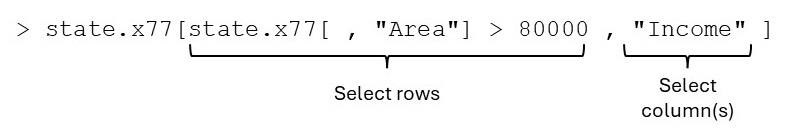
\includegraphics[width=0.8\linewidth]{pics/matrixSubscripting}

\begin{Shaded}
\begin{Highlighting}[]
\NormalTok{x }\OtherTok{\textless{}{-}} \FunctionTok{c}\NormalTok{(}\DecValTok{10}\NormalTok{, }\DecValTok{15}\NormalTok{, }\DecValTok{12}\NormalTok{, }\ConstantTok{NA}\NormalTok{, }\DecValTok{18}\NormalTok{, }\DecValTok{20}\NormalTok{)}
\FunctionTok{is.na}\NormalTok{ (x)}
\CommentTok{\#\textgreater{} [1] FALSE FALSE FALSE  TRUE FALSE FALSE}
\NormalTok{x[}\FunctionTok{is.na}\NormalTok{ (x)]}
\CommentTok{\#\textgreater{} [1] NA}
\NormalTok{x[}\SpecialCharTok{!}\FunctionTok{is.na}\NormalTok{ (x)]}
\CommentTok{\#\textgreater{} [1] 10 15 12 18 20}
\FunctionTok{mean}\NormalTok{ (x)}
\CommentTok{\#\textgreater{} [1] NA}
\FunctionTok{mean}\NormalTok{ (x[}\SpecialCharTok{!}\FunctionTok{is.na}\NormalTok{ (x)])}
\CommentTok{\#\textgreater{} [1] 15}
\FunctionTok{mean}\NormalTok{ (}\FunctionTok{na.omit}\NormalTok{ (x))}
\CommentTok{\#\textgreater{} [1] 15}
\end{Highlighting}
\end{Shaded}

Logical subscripting allows finding the indices of those elements in a vector that meet a certain condition e.g.

\begin{Shaded}
\begin{Highlighting}[]
\NormalTok{(}\DecValTok{1}\SpecialCharTok{:}\FunctionTok{length}\NormalTok{ (}\FunctionTok{rownames}\NormalTok{ (state.x77)))[state.x77[ ,}\StringTok{"Income"}\NormalTok{] }\SpecialCharTok{\textgreater{}} \DecValTok{5000}\NormalTok{]}
\CommentTok{\#\textgreater{} [1]  2  5  7 13 20 28 30 34}
\end{Highlighting}
\end{Shaded}

and to find the corresponding names of the states

\begin{Shaded}
\begin{Highlighting}[]
\FunctionTok{rownames}\NormalTok{(state.x77)[}
\NormalTok{  (}\DecValTok{1}\SpecialCharTok{:}\FunctionTok{length}\NormalTok{ (}\FunctionTok{rownames}\NormalTok{(state.x77)))[state.x77[ ,}\StringTok{"Income"}\NormalTok{] }\SpecialCharTok{\textgreater{}} \DecValTok{5000}\NormalTok{]]}
\CommentTok{\#\textgreater{} [1] "Alaska"       "California"   "Connecticut" }
\CommentTok{\#\textgreater{} [4] "Illinois"     "Maryland"     "Nevada"      }
\CommentTok{\#\textgreater{} [7] "New Jersey"   "North Dakota"}
\end{Highlighting}
\end{Shaded}

In addition to extracting elements, the above subscripting operations can also be used to modify selected elements of a vector e.g.~changing NA-values to zero:

\begin{Shaded}
\begin{Highlighting}[]
\NormalTok{x}
\CommentTok{\#\textgreater{} [1] 10 15 12 NA 18 20}
\NormalTok{x[}\FunctionTok{is.na}\NormalTok{ (x)] }\OtherTok{\textless{}{-}} \DecValTok{0}
\NormalTok{x}
\CommentTok{\#\textgreater{} [1] 10 15 12  0 18 20}
\end{Highlighting}
\end{Shaded}

When the right-hand side of the assignment above is a scalar value, each of the selected values will be changed to the specified scalar value; if the right-hand side is a vector, the selecting values will be changed in order, \emph{{recycling}} the values if more values were selected on the left-hand side than were available on the right-hand side.

\section{Subscripting with matrices}\label{subscripting-with-matrices}

Element and submatrix extraction of matrices are discussed below.

\begin{enumerate}
\def\labelenumi{(\alph{enumi})}
\item
  Revise the use of \texttt{matrix()}, \texttt{names()}, \texttt{dim()} and \texttt{dimnames()}.
\item
  A matrix in R is an \emph{{array}} with two indices. Arrays of order two and higher can be constructed with the function \texttt{dim()} or \texttt{array()}.
\end{enumerate}

Let, for example, \(\mathbf{a}\) be a vector consisting of \(150\) elements. The instruction

\begin{Shaded}
\begin{Highlighting}[]
\FunctionTok{dim}\NormalTok{(a) }\OtherTok{\textless{}{-}} \FunctionTok{c}\NormalTok{(}\DecValTok{3}\NormalTok{, }\DecValTok{5}\NormalTok{, }\DecValTok{10}\NormalTok{) }
\end{Highlighting}
\end{Shaded}

or the instruction

\begin{Shaded}
\begin{Highlighting}[]
\NormalTok{a }\OtherTok{\textless{}{-}} \FunctionTok{array}\NormalTok{ (a, }\AttributeTok{dim =} \FunctionTok{c}\NormalTok{(}\DecValTok{3}\NormalTok{, }\DecValTok{5}\NormalTok{, }\DecValTok{10}\NormalTok{)) }
\end{Highlighting}
\end{Shaded}

constructs a \(3 \times 5 \times 10\) array.

\begin{itemize}
\tightlist
\item
  Matrices can therefore be formed as above, but the function \texttt{matrix()} is usually easier to use.
\item
  The elements of a \(p\)-dimensional array can also be extracted using the one-index or two-index method as described below.
\end{itemize}

\begin{enumerate}
\def\labelenumi{(\alph{enumi})}
\setcounter{enumi}{2}
\item
  The subscripting methods described in section \ref{vectorSubscripting} can also be applied to both the first or second dimension of a matrix where the first dimension refers to the rows and the second dimension to the columns of the matrix.
\item
  Note that the elements of a matrix can be referred to by the two-index method above or by a one index method. When the one index method is used it is assumed that the matrix has first been strung out \emph{{column}}-wise into a vector.
\end{enumerate}

\begin{Shaded}
\begin{Highlighting}[]
\NormalTok{testmat.a }\OtherTok{\textless{}{-}} \FunctionTok{matrix}\NormalTok{ (}\FunctionTok{c}\NormalTok{ (}\DecValTok{17}\NormalTok{, }\DecValTok{40}\NormalTok{, }\DecValTok{20}\NormalTok{, }\DecValTok{34}\NormalTok{, }\DecValTok{21}\NormalTok{, }\DecValTok{12}\NormalTok{, }\DecValTok{14}\NormalTok{, }\DecValTok{57}\NormalTok{, }
                        \DecValTok{78}\NormalTok{, }\DecValTok{37}\NormalTok{, }\DecValTok{29}\NormalTok{, }\DecValTok{64}\NormalTok{), }\AttributeTok{nrow =} \DecValTok{4}\NormalTok{)}
\NormalTok{testmat.a}
\CommentTok{\#\textgreater{}      [,1] [,2] [,3]}
\CommentTok{\#\textgreater{} [1,]   17   21   78}
\CommentTok{\#\textgreater{} [2,]   40   12   37}
\CommentTok{\#\textgreater{} [3,]   20   14   29}
\CommentTok{\#\textgreater{} [4,]   34   57   64}
\NormalTok{testmat.b }\OtherTok{\textless{}{-}} \FunctionTok{matrix}\NormalTok{ (}\FunctionTok{c}\NormalTok{ (}\DecValTok{17}\NormalTok{, }\DecValTok{40}\NormalTok{, }\DecValTok{20}\NormalTok{, }\DecValTok{34}\NormalTok{, }\DecValTok{21}\NormalTok{, }\DecValTok{12}\NormalTok{, }\DecValTok{14}\NormalTok{, }\DecValTok{57}\NormalTok{, }
                        \DecValTok{78}\NormalTok{, }\DecValTok{37}\NormalTok{, }\DecValTok{29}\NormalTok{, }\DecValTok{64}\NormalTok{), }\AttributeTok{nrow =} \DecValTok{4}\NormalTok{, }\AttributeTok{byrow =} \ConstantTok{TRUE}\NormalTok{)}
\NormalTok{testmat.b}
\CommentTok{\#\textgreater{}      [,1] [,2] [,3]}
\CommentTok{\#\textgreater{} [1,]   17   40   20}
\CommentTok{\#\textgreater{} [2,]   34   21   12}
\CommentTok{\#\textgreater{} [3,]   14   57   78}
\CommentTok{\#\textgreater{} [4,]   37   29   64}
\end{Highlighting}
\end{Shaded}

Comment on the difference between \texttt{testmat.a} and \texttt{testmat.b}.

\begin{Shaded}
\begin{Highlighting}[]
\NormalTok{testmat.a[}\DecValTok{2}\NormalTok{,}\DecValTok{3}\NormalTok{]   }\CommentTok{\# Two index matrix reference}
\CommentTok{\#\textgreater{} [1] 37}
\NormalTok{testmat.a[}\DecValTok{10}\NormalTok{]   }\CommentTok{\# One index matrix reference}
\CommentTok{\#\textgreater{} [1] 37}
\end{Highlighting}
\end{Shaded}

\begin{enumerate}
\def\labelenumi{(\alph{enumi})}
\setcounter{enumi}{4}
\item
  Write a function to convert a one-index to a two-index matrix reference. Give an example of the usage of your function.
\item
  Write a function to convert a two-index to a one-index matrix reference. Give an example of the usage of your function.
\end{enumerate}

\begin{enumerate}
\def\labelenumi{(\alph{enumi})}
\setcounter{enumi}{6}
\tightlist
\item
  Consider the following example to form submatrices:
\end{enumerate}

\begin{Shaded}
\begin{Highlighting}[]
\NormalTok{testmat }\OtherTok{\textless{}{-}} \FunctionTok{matrix}\NormalTok{(}\DecValTok{1}\SpecialCharTok{:}\DecValTok{50}\NormalTok{, }\AttributeTok{nrow =} \DecValTok{10}\NormalTok{, }\AttributeTok{byrow =} \ConstantTok{TRUE}\NormalTok{)}
\NormalTok{testmat[}\DecValTok{1}\SpecialCharTok{:}\DecValTok{2}\NormalTok{, }\FunctionTok{c}\NormalTok{ (}\DecValTok{3}\NormalTok{, }\DecValTok{5}\NormalTok{)]}
\CommentTok{\#\textgreater{}      [,1] [,2]}
\CommentTok{\#\textgreater{} [1,]    3    5}
\CommentTok{\#\textgreater{} [2,]    8   10}
\NormalTok{testmat[}\DecValTok{1}\SpecialCharTok{:}\DecValTok{2}\NormalTok{, }\DecValTok{3}\NormalTok{]}
\CommentTok{\#\textgreater{} [1] 3 8}
\NormalTok{testmat[}\DecValTok{1}\SpecialCharTok{:}\DecValTok{2}\NormalTok{, }\DecValTok{3}\NormalTok{, drop}\OtherTok{=}\ConstantTok{FALSE}\NormalTok{]}
\CommentTok{\#\textgreater{}      [,1]}
\CommentTok{\#\textgreater{} [1,]    3}
\CommentTok{\#\textgreater{} [2,]    8}
\end{Highlighting}
\end{Shaded}

\begin{enumerate}
\def\labelenumi{(\alph{enumi})}
\setcounter{enumi}{7}
\item
  Notice the difference between \texttt{testmat\ {[}1:2,\ 3{]}} and \texttt{testmat\ {[}1:2,\ 3,\ drop\ =\ FALSE{]}}. The first command results in the output to be given in the form of a vector while the optional \texttt{drop\ =\ FALSE} in the second command retains the matrix structure of the output. This distinction can have serious consequences when a procedure expects a matrix argument and not a vector.
\item
  Notice also that the output of both \texttt{testmat{[}1:2,3{]}} and \texttt{testmat{[}3,\ 1:2{]}} has a similar form: R makes no distinction between column vectors and row vectors; all one-dimensional collections of numbers are treated identically.
\item
  Apart from using vectors as subscripts to a matrix, a matrix can also be used as a subscript to a matrix. There are two cases:

  \begin{enumerate}
  \def\labelenumii{(\Alph{enumii})}
  \tightlist
  \item
    a numeric subscripting matrix and
  \item
    a logical subscripting matrix.
  \end{enumerate}
\end{enumerate}

\subsubsection*{Case A}\label{case-a}
\addcontentsline{toc}{subsubsection}{Case A}

Here the subscripting numeric matrix must have exactly two columns: the first provide row indices and the second column indices.

\begin{enumerate}
\def\labelenumi{(\roman{enumi})}
\item
  If used on the right-hand side of an expression the result of a \emph{case A} subscripting is a vector containing the values specified by the subscripting matrix.
\item
  If used on the left-hand side of an assignment a numeric matrix first selects those elements specified by its row and column indices; then these values are replaced one by one with the objects specified by the right-hand side of the assignment.
\end{enumerate}

Here is an example of \emph{case A} subscripting with the subscript matrix on the right-hand side of the assignment:

\begin{Shaded}
\begin{Highlighting}[]
\NormalTok{xmat }\OtherTok{\textless{}{-}} \FunctionTok{matrix}\NormalTok{ (}\DecValTok{1}\SpecialCharTok{:}\DecValTok{25}\NormalTok{, }\AttributeTok{nrow =} \DecValTok{5}\NormalTok{)}
\NormalTok{xmat}
\CommentTok{\#\textgreater{}      [,1] [,2] [,3] [,4] [,5]}
\CommentTok{\#\textgreater{} [1,]    1    6   11   16   21}
\CommentTok{\#\textgreater{} [2,]    2    7   12   17   22}
\CommentTok{\#\textgreater{} [3,]    3    8   13   18   23}
\CommentTok{\#\textgreater{} [4,]    4    9   14   19   24}
\CommentTok{\#\textgreater{} [5,]    5   10   15   20   25}
\NormalTok{superdiag.index }\OtherTok{\textless{}{-}} \FunctionTok{matrix}\NormalTok{ (}\FunctionTok{c}\NormalTok{ (}\DecValTok{1}\SpecialCharTok{:}\DecValTok{4}\NormalTok{, }\DecValTok{2}\SpecialCharTok{:}\DecValTok{5}\NormalTok{), }\AttributeTok{ncol =} \DecValTok{2}\NormalTok{, }\AttributeTok{byrow =} \ConstantTok{FALSE}\NormalTok{)}
\NormalTok{superdiag.values }\OtherTok{\textless{}{-}}\NormalTok{ xmat[superdiag.index]}
\NormalTok{superdiag.values}
\CommentTok{\#\textgreater{} [1]  6 12 18 24}
\end{Highlighting}
\end{Shaded}

\emph{Case A} subscripting with the numeric subscript matrix on the left-hand side of the assignment:

\begin{Shaded}
\begin{Highlighting}[]
\NormalTok{subscript.mat }\OtherTok{\textless{}{-}} \FunctionTok{matrix}\NormalTok{ (}\FunctionTok{c}\NormalTok{(}\DecValTok{1}\SpecialCharTok{:}\DecValTok{3}\NormalTok{, }\DecValTok{1}\SpecialCharTok{:}\DecValTok{3}\NormalTok{, }\FunctionTok{rep}\NormalTok{(}\DecValTok{1}\NormalTok{,}\DecValTok{3}\NormalTok{), }\FunctionTok{rep}\NormalTok{(}\DecValTok{2}\NormalTok{,}\DecValTok{3}\NormalTok{)), }\AttributeTok{ncol=}\DecValTok{2}\NormalTok{)}
\NormalTok{subscript.mat}
\CommentTok{\#\textgreater{}      [,1] [,2]}
\CommentTok{\#\textgreater{} [1,]    1    1}
\CommentTok{\#\textgreater{} [2,]    2    1}
\CommentTok{\#\textgreater{} [3,]    3    1}
\CommentTok{\#\textgreater{} [4,]    1    2}
\CommentTok{\#\textgreater{} [5,]    2    2}
\CommentTok{\#\textgreater{} [6,]    3    2}
\NormalTok{xx }\OtherTok{\textless{}{-}} \FunctionTok{matrix}\NormalTok{(}\ConstantTok{NA}\NormalTok{, }\AttributeTok{nrow=}\DecValTok{3}\NormalTok{,}\AttributeTok{ncol=}\DecValTok{2}\NormalTok{)}
\NormalTok{xx }
\CommentTok{\#\textgreater{}      [,1] [,2]}
\CommentTok{\#\textgreater{} [1,]   NA   NA}
\CommentTok{\#\textgreater{} [2,]   NA   NA}
\CommentTok{\#\textgreater{} [3,]   NA   NA}
\NormalTok{xx[subscript.mat] }\OtherTok{\textless{}{-}} \FunctionTok{c}\NormalTok{(}\DecValTok{10}\NormalTok{,}\DecValTok{12}\NormalTok{,}\DecValTok{14}\NormalTok{,}\DecValTok{100}\NormalTok{,}\DecValTok{120}\NormalTok{,}\DecValTok{140}\NormalTok{)}
\NormalTok{xx}
\CommentTok{\#\textgreater{}      [,1] [,2]}
\CommentTok{\#\textgreater{} [1,]   10  100}
\CommentTok{\#\textgreater{} [2,]   12  120}
\CommentTok{\#\textgreater{} [3,]   14  140}
\end{Highlighting}
\end{Shaded}

\subsubsection*{Case B}\label{case-b}
\addcontentsline{toc}{subsubsection}{Case B}

The logical subscripting matrix must be in size exactly similar to that matrix it is subscripting and will select those values corresponding to a \texttt{TRUE} in the subscripting matrix.

\emph{Case B} with logical subscripting matrix at right-hand side of assignment:

\begin{Shaded}
\begin{Highlighting}[]
\NormalTok{testmat}
\CommentTok{\#\textgreater{}       [,1] [,2] [,3] [,4] [,5]}
\CommentTok{\#\textgreater{}  [1,]    1    2    3    4    5}
\CommentTok{\#\textgreater{}  [2,]    6    7    8    9   10}
\CommentTok{\#\textgreater{}  [3,]   11   12   13   14   15}
\CommentTok{\#\textgreater{}  [4,]   16   17   18   19   20}
\CommentTok{\#\textgreater{}  [5,]   21   22   23   24   25}
\CommentTok{\#\textgreater{}  [6,]   26   27   28   29   30}
\CommentTok{\#\textgreater{}  [7,]   31   32   33   34   35}
\CommentTok{\#\textgreater{}  [8,]   36   37   38   39   40}
\CommentTok{\#\textgreater{}  [9,]   41   42   43   44   45}
\CommentTok{\#\textgreater{} [10,]   46   47   48   49   50}
\NormalTok{aa }\OtherTok{\textless{}{-}}\NormalTok{ testmat[testmat }\SpecialCharTok{\textless{}} \DecValTok{12}\NormalTok{]}
\NormalTok{aa}
\CommentTok{\#\textgreater{}  [1]  1  6 11  2  7  3  8  4  9  5 10}
\end{Highlighting}
\end{Shaded}

Note that the selected elements are placed column-wise in a vector.

\emph{Case B} with logical subscripting matrix at left-hand side of assignment:

\begin{Shaded}
\begin{Highlighting}[]
\NormalTok{testmat[testmat }\SpecialCharTok{\textless{}} \DecValTok{12}\NormalTok{] }\OtherTok{\textless{}{-}} \DecValTok{12}
\NormalTok{testmat}
\CommentTok{\#\textgreater{}       [,1] [,2] [,3] [,4] [,5]}
\CommentTok{\#\textgreater{}  [1,]   12   12   12   12   12}
\CommentTok{\#\textgreater{}  [2,]   12   12   12   12   12}
\CommentTok{\#\textgreater{}  [3,]   12   12   13   14   15}
\CommentTok{\#\textgreater{}  [4,]   16   17   18   19   20}
\CommentTok{\#\textgreater{}  [5,]   21   22   23   24   25}
\CommentTok{\#\textgreater{}  [6,]   26   27   28   29   30}
\CommentTok{\#\textgreater{}  [7,]   31   32   33   34   35}
\CommentTok{\#\textgreater{}  [8,]   36   37   38   39   40}
\CommentTok{\#\textgreater{}  [9,]   41   42   43   44   45}
\CommentTok{\#\textgreater{} [10,]   46   47   48   49   50}
\end{Highlighting}
\end{Shaded}

In order to restrict assignment to a subset of a matrix two sets of subscripts are needed. See example below:

\begin{Shaded}
\begin{Highlighting}[]
\NormalTok{testmat }\OtherTok{\textless{}{-}} \FunctionTok{matrix}\NormalTok{(}\DecValTok{1}\SpecialCharTok{:}\DecValTok{50}\NormalTok{, }\AttributeTok{nrow=}\DecValTok{10}\NormalTok{, }\AttributeTok{byrow=}\ConstantTok{TRUE}\NormalTok{)}
\NormalTok{testmat[, }\FunctionTok{c}\NormalTok{(}\DecValTok{1}\NormalTok{,}\DecValTok{3}\NormalTok{)][testmat[,}\FunctionTok{c}\NormalTok{(}\DecValTok{1}\NormalTok{,}\DecValTok{3}\NormalTok{)] }\SpecialCharTok{\textless{}}\DecValTok{12}\NormalTok{] }\OtherTok{\textless{}{-}} \DecValTok{12}
\NormalTok{testmat}
\CommentTok{\#\textgreater{}       [,1] [,2] [,3] [,4] [,5]}
\CommentTok{\#\textgreater{}  [1,]   12    2   12    4    5}
\CommentTok{\#\textgreater{}  [2,]   12    7   12    9   10}
\CommentTok{\#\textgreater{}  [3,]   12   12   13   14   15}
\CommentTok{\#\textgreater{}  [4,]   16   17   18   19   20}
\CommentTok{\#\textgreater{}  [5,]   21   22   23   24   25}
\CommentTok{\#\textgreater{}  [6,]   26   27   28   29   30}
\CommentTok{\#\textgreater{}  [7,]   31   32   33   34   35}
\CommentTok{\#\textgreater{}  [8,]   36   37   38   39   40}
\CommentTok{\#\textgreater{}  [9,]   41   42   43   44   45}
\CommentTok{\#\textgreater{} [10,]   46   47   48   49   50}
\end{Highlighting}
\end{Shaded}

Study the use of functions \texttt{row()} and \texttt{col()} in constructing logical matrices.

\section{Extracting elements of lists}\label{extracting-elements-of-lists}

\begin{enumerate}
\def\labelenumi{(\alph{enumi})}
\tightlist
\item
  Note the use of \texttt{list()} to collect objects into a list while elements are extracted with \texttt{\$}
\end{enumerate}

\begin{itemize}
\item
  the function \texttt{names()},
\item
  the single square brackets \texttt{{[}\ {]}} and
\item
  the double square brackets \texttt{{[}{[}\ {]}{]}}.
\end{itemize}

\begin{enumerate}
\def\labelenumi{(\alph{enumi})}
\setcounter{enumi}{1}
\tightlist
\item
  Study the following example carefully:
\end{enumerate}

\begin{Shaded}
\begin{Highlighting}[]
\NormalTok{my.list }\OtherTok{\textless{}{-}} \FunctionTok{list}\NormalTok{(}\AttributeTok{el1 =} \DecValTok{1}\SpecialCharTok{:}\DecValTok{5}\NormalTok{, }
                \AttributeTok{el2 =} \FunctionTok{c}\NormalTok{(}\StringTok{"a"}\NormalTok{, }\StringTok{"b"}\NormalTok{, }\StringTok{"c"}\NormalTok{), }
                \AttributeTok{el3 =} \FunctionTok{matrix}\NormalTok{(}\DecValTok{1}\SpecialCharTok{:}\DecValTok{16}\NormalTok{, }\AttributeTok{ncol =} \DecValTok{4}\NormalTok{), }
                \AttributeTok{el4 =} \FunctionTok{c}\NormalTok{(}\DecValTok{12}\NormalTok{, }\DecValTok{17}\NormalTok{, }\DecValTok{23}\NormalTok{, }\DecValTok{9}\NormalTok{))}
\NormalTok{my.list}
\CommentTok{\#\textgreater{} $el1}
\CommentTok{\#\textgreater{} [1] 1 2 3 4 5}
\CommentTok{\#\textgreater{} }
\CommentTok{\#\textgreater{} $el2}
\CommentTok{\#\textgreater{} [1] "a" "b" "c"}
\CommentTok{\#\textgreater{} }
\CommentTok{\#\textgreater{} $el3}
\CommentTok{\#\textgreater{}      [,1] [,2] [,3] [,4]}
\CommentTok{\#\textgreater{} [1,]    1    5    9   13}
\CommentTok{\#\textgreater{} [2,]    2    6   10   14}
\CommentTok{\#\textgreater{} [3,]    3    7   11   15}
\CommentTok{\#\textgreater{} [4,]    4    8   12   16}
\CommentTok{\#\textgreater{} }
\CommentTok{\#\textgreater{} $el4}
\CommentTok{\#\textgreater{} [1] 12 17 23  9}
\NormalTok{my.list}\SpecialCharTok{$}\NormalTok{el2}
\CommentTok{\#\textgreater{} [1] "a" "b" "c"}
\FunctionTok{mode}\NormalTok{ (my.list}\SpecialCharTok{$}\NormalTok{el2)}
\CommentTok{\#\textgreater{} [1] "character"}
\NormalTok{my.list[el2]}
\CommentTok{\#\textgreater{} Error: object \textquotesingle{}el2\textquotesingle{} not found}
\NormalTok{my.list[}\StringTok{"el2"}\NormalTok{]}
\CommentTok{\#\textgreater{} $el2}
\CommentTok{\#\textgreater{} [1] "a" "b" "c"}
\FunctionTok{mode}\NormalTok{ (my.list[}\StringTok{"el2"}\NormalTok{])}
\CommentTok{\#\textgreater{} [1] "list"}
\NormalTok{my.list[[}\StringTok{"el2"}\NormalTok{]]}
\CommentTok{\#\textgreater{} [1] "a" "b" "c"}
\FunctionTok{mode}\NormalTok{ (my.list[[}\StringTok{"el2"}\NormalTok{]])}
\CommentTok{\#\textgreater{} [1] "character"}
\end{Highlighting}
\end{Shaded}

Note: The above example shows that using the single pair of square brackets for subscripting a list always result in a list object to be returned. This is often the cause of an error message. See the example below.

\begin{Shaded}
\begin{Highlighting}[]
\NormalTok{my.list[}\DecValTok{1}\NormalTok{]}
\CommentTok{\#\textgreater{} $el1}
\CommentTok{\#\textgreater{} [1] 1 2 3 4 5}
\FunctionTok{mode}\NormalTok{ (my.list[}\DecValTok{1}\NormalTok{])}
\CommentTok{\#\textgreater{} [1] "list"}
\NormalTok{my.list[[}\DecValTok{1}\NormalTok{]]}
\CommentTok{\#\textgreater{} [1] 1 2 3 4 5}
\FunctionTok{mode}\NormalTok{ (my.list[[}\DecValTok{1}\NormalTok{]])}
\CommentTok{\#\textgreater{} [1] "numeric"}
\NormalTok{my.list[}\DecValTok{3}\NormalTok{][}\DecValTok{2}\NormalTok{,}\DecValTok{4}\NormalTok{]}
\CommentTok{\#\textgreater{} Error in my.list[3][2, 4]: incorrect number of dimensions}
\NormalTok{my.list[[}\DecValTok{3}\NormalTok{]][}\DecValTok{2}\NormalTok{,}\DecValTok{4}\NormalTok{]}
\CommentTok{\#\textgreater{} [1] 14}
\NormalTok{my.list}\SpecialCharTok{$}\NormalTok{el3[}\DecValTok{2}\NormalTok{,}\DecValTok{4}\NormalTok{]}
\CommentTok{\#\textgreater{} [1] 14}
\FunctionTok{mean}\NormalTok{ (my.list[}\DecValTok{4}\NormalTok{])}
\CommentTok{\#\textgreater{} Warning in mean.default(my.list[4]): argument is not}
\CommentTok{\#\textgreater{} numeric or logical: returning NA}
\CommentTok{\#\textgreater{} [1] NA}
\FunctionTok{mean}\NormalTok{ (my.list[[}\DecValTok{4}\NormalTok{]])}
\CommentTok{\#\textgreater{} [1] 15.25}
\FunctionTok{mean}\NormalTok{ (my.list}\SpecialCharTok{$}\NormalTok{el4)}
\CommentTok{\#\textgreater{} [1] 15.25}
\end{Highlighting}
\end{Shaded}

Explain the differences and similarities between the symbols \texttt{{[}\ {]}}, \texttt{{[}{[}\ {]}{]}} and \texttt{\$} when subscripting lists.

\section{Extracting elements from dataframes}\label{extracting-elements-from-dataframes}

\begin{enumerate}
\def\labelenumi{(\alph{enumi})}
\item
  Note the use of data.frame() for creating dataframes. A dataframe has a rectangular structure similar to a matrix but differs from a matrix in that its columns are not restricted to contain the same type of data. Each of its columns must contain the same sort of data but some columns can be numerical while others are factors for example.
\item
  Explain the difference between the objects created by the following two instructions:
\end{enumerate}

\begin{Shaded}
\begin{Highlighting}[]
\NormalTok{my.matrix }\OtherTok{\textless{}{-}} \FunctionTok{matrix}\NormalTok{ (}\FunctionTok{c}\NormalTok{ (}\DecValTok{17}\NormalTok{, }\DecValTok{40}\NormalTok{, }\DecValTok{20}\NormalTok{, }\DecValTok{34}\NormalTok{, }\DecValTok{21}\NormalTok{, }\DecValTok{12}\NormalTok{, }\DecValTok{14}\NormalTok{, }\DecValTok{57}\NormalTok{,}
                        \DecValTok{78}\NormalTok{, }\DecValTok{37}\NormalTok{, }\DecValTok{29}\NormalTok{, }\DecValTok{64}\NormalTok{), }\AttributeTok{nrow =} \DecValTok{4}\NormalTok{, }\AttributeTok{ncol =} \DecValTok{3}\NormalTok{)}
\NormalTok{my.dataframe }\OtherTok{\textless{}{-}} \FunctionTok{data.frame}\NormalTok{ ( }\FunctionTok{c}\NormalTok{(}\DecValTok{17}\NormalTok{, }\DecValTok{40}\NormalTok{, }\DecValTok{20}\NormalTok{, }\DecValTok{34}\NormalTok{, }\DecValTok{21}\NormalTok{, }\DecValTok{12}\NormalTok{, }\DecValTok{14}\NormalTok{, }\DecValTok{57}\NormalTok{,}
                               \DecValTok{78}\NormalTok{, }\DecValTok{37}\NormalTok{, }\DecValTok{29}\NormalTok{, }\DecValTok{64}\NormalTok{), }\AttributeTok{nrow =} \DecValTok{4}\NormalTok{, }\AttributeTok{ncol =} \DecValTok{3}\NormalTok{)}
\end{Highlighting}
\end{Shaded}

\begin{enumerate}
\def\labelenumi{(\alph{enumi})}
\setcounter{enumi}{2}
\tightlist
\item
  Note the following
\end{enumerate}

\begin{Shaded}
\begin{Highlighting}[]
\FunctionTok{class}\NormalTok{(my.matrix)}
\CommentTok{\#\textgreater{} [1] "matrix" "array"}
\FunctionTok{class}\NormalTok{(my.dataframe)}
\CommentTok{\#\textgreater{} [1] "data.frame"}
\FunctionTok{is.list}\NormalTok{(data.frame)}
\CommentTok{\#\textgreater{} [1] FALSE}
\FunctionTok{mode}\NormalTok{(my.matrix)}
\CommentTok{\#\textgreater{} [1] "numeric"}
\FunctionTok{mode}\NormalTok{(data.frame)}
\CommentTok{\#\textgreater{} [1] "function"}
\end{Highlighting}
\end{Shaded}

\begin{enumerate}
\def\labelenumi{(\alph{enumi})}
\setcounter{enumi}{3}
\tightlist
\item
  A sample of the behaviour of dataframes
\end{enumerate}

\begin{Shaded}
\begin{Highlighting}[]
\NormalTok{my.dataframe}\FloatTok{.2} \OtherTok{\textless{}{-}} \FunctionTok{data.frame}\NormalTok{ (}\AttributeTok{C1 =} \FunctionTok{c}\NormalTok{(}\StringTok{\textquotesingle{}a\textquotesingle{}}\NormalTok{, }\StringTok{\textquotesingle{}b\textquotesingle{}}\NormalTok{, }\StringTok{\textquotesingle{}c\textquotesingle{}}\NormalTok{, }\StringTok{\textquotesingle{}d\textquotesingle{}}\NormalTok{), }
                              \AttributeTok{C2 =} \FunctionTok{c}\NormalTok{(}\DecValTok{5}\NormalTok{, }\DecValTok{9}\NormalTok{, }\DecValTok{23}\NormalTok{, }\DecValTok{17}\NormalTok{), }
                              \AttributeTok{C3 =} \FunctionTok{c}\NormalTok{(}\ConstantTok{TRUE}\NormalTok{, }\ConstantTok{TRUE}\NormalTok{, }\ConstantTok{FALSE}\NormalTok{, }\ConstantTok{TRUE}\NormalTok{))}
\NormalTok{my.dataframe}\FloatTok{.2}
\CommentTok{\#\textgreater{}   C1 C2    C3}
\CommentTok{\#\textgreater{} 1  a  5  TRUE}
\CommentTok{\#\textgreater{} 2  b  9  TRUE}
\CommentTok{\#\textgreater{} 3  c 23 FALSE}
\CommentTok{\#\textgreater{} 4  d 17  TRUE}
\NormalTok{my.dataframe}\FloatTok{.2}\NormalTok{[ ,}\DecValTok{1}\SpecialCharTok{:}\DecValTok{2}\NormalTok{]}
\CommentTok{\#\textgreater{}   C1 C2}
\CommentTok{\#\textgreater{} 1  a  5}
\CommentTok{\#\textgreater{} 2  b  9}
\CommentTok{\#\textgreater{} 3  c 23}
\CommentTok{\#\textgreater{} 4  d 17}
\end{Highlighting}
\end{Shaded}

Dataframe behaves like a matrix

\begin{Shaded}
\begin{Highlighting}[]
\NormalTok{my.dataframe}\FloatTok{.2}\SpecialCharTok{$}\NormalTok{C1}
\CommentTok{\#\textgreater{} [1] "a" "b" "c" "d"}
\end{Highlighting}
\end{Shaded}

Dataframe behaves like a list

\begin{Shaded}
\begin{Highlighting}[]
\FunctionTok{as.matrix}\NormalTok{(my.dataframe}\FloatTok{.2}\NormalTok{)}
\CommentTok{\#\textgreater{}      C1  C2   C3     }
\CommentTok{\#\textgreater{} [1,] "a" " 5" "TRUE" }
\CommentTok{\#\textgreater{} [2,] "b" " 9" "TRUE" }
\CommentTok{\#\textgreater{} [3,] "c" "23" "FALSE"}
\CommentTok{\#\textgreater{} [4,] "d" "17" "TRUE"}
\end{Highlighting}
\end{Shaded}

Explain what has happened above.

\begin{enumerate}
\def\labelenumi{(\alph{enumi})}
\setcounter{enumi}{4}
\item
  The above examples show that a dataframe can be considered as a cross between a matrix and a list. Therefore, subscripting of dataframes generally can be performed using the basic techniques available for matrices and lists.
\item
  An alternative technique is to extract the elements of a list by using the functions \texttt{attach()} and \texttt{names()}. This technique is especially of importance in statistical modelling. What is a potential danger of this technique when attaching dataframes? This danger can be avoided by using \texttt{with()}. Is this also true when modelling is performed?
\item
  Review section \ref{findData}. Study the help file of the function \texttt{with()}. What important usage has \texttt{with()}?
\end{enumerate}

\section{Combining vectors, matrices, lists and dataframes}\label{combining-vectors-matrices-lists-and-dataframes}

\begin{enumerate}
\def\labelenumi{(\alph{enumi})}
\tightlist
\item
  What is the result of the command
\end{enumerate}

\begin{Shaded}
\begin{Highlighting}[]
\NormalTok{my.list }\OtherTok{\textless{}{-}} \FunctionTok{vector}\NormalTok{ (}\StringTok{"list"}\NormalTok{, k)?}
\end{Highlighting}
\end{Shaded}

\begin{enumerate}
\def\labelenumi{(\alph{enumi})}
\setcounter{enumi}{1}
\item
  Recall the function \texttt{c()} for creating vectors. When \texttt{c()} is used to combine a numeric vector and a character vector the result is a vector of mode ``character''. Similarly, using \texttt{c()} to combine a vector with a list results in a list.
\item
  If \texttt{list()} is used to combine two or more vectors or lists the result is a list of all the objects.
\item
  The function \texttt{unlist()} can be used to convert all the elements of a list into a single vector.
\end{enumerate}

\begin{Shaded}
\begin{Highlighting}[]
\NormalTok{my.list}
\CommentTok{\#\textgreater{} $el1}
\CommentTok{\#\textgreater{} [1] 1 2 3 4 5}
\CommentTok{\#\textgreater{} }
\CommentTok{\#\textgreater{} $el2}
\CommentTok{\#\textgreater{} [1] "a" "b" "c"}
\CommentTok{\#\textgreater{} }
\CommentTok{\#\textgreater{} $el3}
\CommentTok{\#\textgreater{}      [,1] [,2] [,3] [,4]}
\CommentTok{\#\textgreater{} [1,]    1    5    9   13}
\CommentTok{\#\textgreater{} [2,]    2    6   10   14}
\CommentTok{\#\textgreater{} [3,]    3    7   11   15}
\CommentTok{\#\textgreater{} [4,]    4    8   12   16}
\CommentTok{\#\textgreater{} }
\CommentTok{\#\textgreater{} $el4}
\CommentTok{\#\textgreater{} [1] 12 17 23  9}
\FunctionTok{unlist}\NormalTok{(my.list)}
\CommentTok{\#\textgreater{}  el11  el12  el13  el14  el15  el21  el22  el23  el31  el32 }
\CommentTok{\#\textgreater{}   "1"   "2"   "3"   "4"   "5"   "a"   "b"   "c"   "1"   "2" }
\CommentTok{\#\textgreater{}  el33  el34  el35  el36  el37  el38  el39 el310 el311 el312 }
\CommentTok{\#\textgreater{}   "3"   "4"   "5"   "6"   "7"   "8"   "9"  "10"  "11"  "12" }
\CommentTok{\#\textgreater{} el313 el314 el315 el316  el41  el42  el43  el44 }
\CommentTok{\#\textgreater{}  "13"  "14"  "15"  "16"  "12"  "17"  "23"   "9"}
\end{Highlighting}
\end{Shaded}

Explain the above output.

\begin{enumerate}
\def\labelenumi{(\alph{enumi})}
\setcounter{enumi}{4}
\tightlist
\item
  Review the functions \texttt{cbind()}, \texttt{rbind()}, \texttt{append()}, \texttt{data.frame()}, \texttt{dim()}, \texttt{dimnames()}, \texttt{names()}, \texttt{colnames()}, \texttt{rownames()}, \texttt{nrow()} and \texttt{ncol()}.
\end{enumerate}

\section{Rearranging the elements in a matrix}\label{rearranging-the-elements-in-a-matrix}

Study the usage of the functions \texttt{matrix()}, \texttt{t()} and \texttt{diag()}. These functions are useful to form submatrices of a matrix or to rearrange matrix elements. Note again the argument \texttt{byrow\ =} of \texttt{matrix()}.

\section{Exercise}\label{exercise-10}

\begin{enumerate}
\def\labelenumi{\arabic{enumi}.}
\item
  Write an R function to check if a given matrix is symmetric.
\item
  Write an R function to extract (i) the row(s) and (ii) the columns containing the maximum value in the matrix. Note that provision must be made that the maximum value can occur in more than one row (column). Furthermore, both the indices and actual values of the rows (columns) must be returned. Illustrate the usage of your function with a suitable example.
\item
  Describe the variables in the built-in data set \texttt{LifeCycleSavings}. Is this data set in the form of a matrix or a dataframe?
\item
  Use subscripting to find the largest proportion of over 75 in those countries with a dpi of less than 1000 in the \texttt{LifeCycleSavings} data set. Also determine the country(ies) having this pop75 value.
\item
  Consider the \texttt{LifeCycleSavings} data set.

  \begin{enumerate}
  \def\labelenumii{(\roman{enumii})}
  \tightlist
  \item
    Use subscripting to find the mean aggregate savings for countries with a percentage of the population younger than 15 at least 10 times the percentage of the population over 75.
  \item
    Also find the mean aggregate savings for countries where the above ratio is less than 10.
  \item
    Use function \texttt{t.test()} to test if mean aggregate savings are different for the above two groups.
  \item
    Use notched box plots for an approximate test.
  \end{enumerate}
\end{enumerate}

\begin{enumerate}
\def\labelenumi{(\alph{enumi})}
\setcounter{enumi}{21}
\tightlist
\item
  First, carefully study the output obtained in (iii) and (iv). Then interpret/discuss this output in detail.
\end{enumerate}

\begin{enumerate}
\def\labelenumi{\arabic{enumi}.}
\setcounter{enumi}{5}
\tightlist
\item
  Consider the \texttt{state.x77} data set and the variable \texttt{state.region}. Find the state with the minimum income in each of the regions defined in state.region.
\end{enumerate}

\chapter{Revision tasks}\label{revision}

In general, the purpose of writing a program in R is to address some practical problem directly or indirectly. To prepare the student for seriously writing R functions (programs) this chapter consists of a mixture of revision tasks. While some of these tasks are straight forward others need more thought and preparation before starting with the writing of R code. In Section \ref{guidelines} some guidelines are considered for writing R code to address a practical problem.

\section{Guidelines for problem solving by writing R code}\label{guidelines}

\begin{enumerate}
\def\labelenumi{(\alph{enumi})}
\item
  Make sure the problem is clearly understood. You cannot write good code for something that is not correctly grasped.
\item
  Break complex problems into simpler components. Formulate these simpler components in terms of specific questions to be answered.
\item
  Think in terms of the way R operates e.g.~vectorized arithmetic, recycling principle, operating on objects as wholes/units, subscripting, R data structures . . .
\item
  Spend time to prepare your data.
\item
  Ask yourself the question what information do you need before attempting to write code for coming up with an answer. Then, what facilities are provided in R to get the necessary information and once the information is available what manipulations are needed to code useful output.
\item
  Write dedicated code for answering the specific questions in (b).
\item
  Do not neglect the debugging/optimizing phase of code that succeeds in providing a first round answer.
\end{enumerate}

\section{Exercise}\label{Ex6}

\begin{enumerate}
\def\labelenumi{\arabic{enumi}.}
\item
  Use R to obtain a five-point summary of the variable \texttt{dpi} in the \texttt{LifeCycleSavings} data set. Illustrate the difference between the working of \texttt{fivenum()} and \texttt{quantile()}. \emph{Hint}: See \texttt{boxplot.stats()} for the definition of hinges.
\item
  Display the pdf of a \(normal (100, 15)\) distribution graphically. The area under the density bounded by the 70th and 90th percentiles must appear in red.
\item
  Use R to obtain the following graphical representations:

  \begin{enumerate}
  \def\labelenumii{(\roman{enumii})}
  \item
    The pdf as well as the cdf of a \(F (15, 10)\) and a \(F (10, 15)\) stochastic variable. These graphs must be on one graph window with the same set of axes for both F-distributions and be supplied with suitable titles. Furthermore, they must be line graphs that contain no other plotting characters except lines.
  \item
    Obtain representations as line graphs of the inverses of the above cdfs on a single separate graph page.
  \end{enumerate}
\item
  First set the seed to 172389 and then generate a random sample of size 500 from a \(normal (100, 20)\) distribution. Give the necessary R instructions to determine the class frequencies in the class intervals ``Smaller than 50'', ``50 to 75--``, ``75 to 90--``, ``90 to 100'', ``100+ to 110'', ``Larger than 110''.
\item
  Generate a random sample of size 80 from a bivariate normal distribution with mean vector \((50, 100)\). The variances of the two variables are 900 and 2500 respectively with a correlation 0.90. Store the sample in an R matrix object and obtain a scatterplot in the form of

  \begin{enumerate}
  \def\labelenumii{(\roman{enumii})}
  \tightlist
  \item
    a point diagram and
  \item
    a line graph of the sample.
  \end{enumerate}
\item
  Define the harmonic mean for a vector of observations. What conditions must be satisfied by the observations?

  \begin{enumerate}
  \def\labelenumii{(\roman{enumii})}
  \item
    Write your own function for calculating a harmonic mean and use it to calculate the harmonic mean of variable \texttt{dpi} in the \texttt{LifeCycleSavings} data set.
  \item
    Calculate the ordinary mean of variable \texttt{dpi} in the \texttt{LifeCycleSavings} data set. Compare the answer with the answer in (a). Which answer would you use in practice? Motivate.
  \end{enumerate}
\item
  Fisher's linear discriminant function in the case of two groups is defined as follows:
\end{enumerate}

\(LDF = (\mathbf{\bar{x}}_1 - \mathbf{\bar{x}}_2)' \mathbf{S}^{-1} \mathbf{x}\) where \(\mathbf{S} = [(n_1-1)\mathbf{S}_1 + (n_2-1)\mathbf{S}_2]/(n_1 + n_2 - 2)\) with \(\mathbf{\bar{x}}_i\) and \(\mathbf{S}_i\) the vector of means and the covariance matrix of the \(i\)th group (sample), respectively.

The corresponding classification function is written as \(CF =(\mathbf{\bar{x}}_1 - \mathbf{\bar{x}}_2)' \mathbf{S}^{-1} \mathbf{x} - \frac{1}{2} (\mathbf{\bar{x}}_1 - \mathbf{\bar{x}}_2)' \mathbf{S}^{-1} (\mathbf{\bar{x}}_1 + \mathbf{\bar{x}}_2)\). The expression \((\mathbf{\bar{x}}_1 - \mathbf{\bar{x}}_2)' \mathbf{S}^{-1}\) is referred to as the discriminant coefficients.

In agreement with section \ref{guidelines} make sure what an \(LDF\) and a \(CF\) entail. The \texttt{crabs} data set in package \texttt{MASS} consists of 200 rows and 8 columns, describing 5 morphological measurements on 50 crabs each of two colour forms and both sexes, of the species \emph{Leptograpsus variegatus} collected at Fremantle, Western Australia.

\begin{enumerate}
\def\labelenumi{(\roman{enumi})}
\item
  Obtain the covariance matrix for each of the two species of crabs.
\item
  Obtain the vector of means for each of the two species of crabs.
\item
  Use standard R functions operating on matrices to write a function or code that calculates the discriminant coefficients for the given linear discriminant function.
\item
  Write a function that determines the linear discriminant function and return
\end{enumerate}

\begin{itemize}
\item
  the discriminant coefficients;
\item
  The CF for each observation.
\end{itemize}

\begin{enumerate}
\def\labelenumi{(\alph{enumi})}
\setcounter{enumi}{21}
\tightlist
\item
  Repeat the discriminant analysis above, discriminating between male and female crabs, ignoring differences in species.
\end{enumerate}

\begin{enumerate}
\def\labelenumi{(\roman{enumi})}
\setcounter{enumi}{5}
\tightlist
\item
  Compare your results to using the \texttt{lda()} function in the package \texttt{MASS} with the command
\end{enumerate}

\begin{Shaded}
\begin{Highlighting}[]
\FunctionTok{predict}\NormalTok{ (}\FunctionTok{lda}\NormalTok{ (sex }\SpecialCharTok{\textasciitilde{}}\NormalTok{ FL }\SpecialCharTok{+}\NormalTok{ RW }\SpecialCharTok{+}\NormalTok{ CL }\SpecialCharTok{+}\NormalTok{ CW }\SpecialCharTok{+}\NormalTok{ BD, }\AttributeTok{data=}\NormalTok{crabs))}\SpecialCharTok{$}\NormalTok{class}
\end{Highlighting}
\end{Shaded}

\begin{enumerate}
\def\labelenumi{\arabic{enumi}.}
\setcounter{enumi}{7}
\tightlist
\item
  Consider the matrix \(\mathbf{A}:n \times m\). What is understood by the column space \(V(\mathbf{A})\) and the orthogonal complement \(V^⊥(\mathbf{A})\)? The R function \texttt{svd()} can be used to obtain an orthogonal basis for \(V(\mathbf{A})\) when the rank of \(\mathbf{A}\) is \(k\). We also want to determine an orthogonal basis for \(V^⊥(\mathbf{A})\). How can the function \texttt{svd()} be used to simultaneously find a basis for \(V(\mathbf{A})\) and for \(V^⊥(\mathbf{A})\)?
\end{enumerate}

The above propositions can be proved as follows: Assume that \(n≥m\) and that an orthonormal basis for \(V(\mathbf{A})\) as well as for \(V^⊥(\mathbf{A})\) must be found. Append \(n-m\) zero vectors of size \(n\) to the matrix \(\mathbf{A}\). Write \(\mathbf{A}^0\) for the appended matrix and perform the function \texttt{svd()} on \(\mathbf{A}^0\). It follows that \(\mathbf{A}^0 = \mathbf{UDV}'\) so that \(\mathbf{A}^0 \mathbf{V} = \mathbf{UD}\), i.e.~

\[
\begin{bmatrix} 
\mathbf{A}^0 \mathbf{v}_{(1)} & \mathbf{A}^0 \mathbf{v}_{(2)} & \dots & \mathbf{A}^0 \mathbf{v}_{(n)}
\end{bmatrix} = \begin{bmatrix} 
d_1 \mathbf{u}_{(1)} & d_2 \mathbf{u}_{(2)} & \dots & d_n \mathbf{u}_{(n)}
\end{bmatrix}.
\]
Now \(\mathbf{A}^0 \mathbf{v}_{(i)} \in V(\mathbf{A}^0) = V(\mathbf{A})\). (\emph{Motivate in detail}.) It follows that \(\mathbf{u}_{(i)} \in V(\mathbf{A}), i = 1, 2, \dots, k\) . (\emph{Motivate in detail}.) Therefore the columns of \(\mathbf{U}\) that correspond to the non-zero \(d\)s form an orthonormal basis for \(V(\mathbf{A})\) while the columns of \(\mathbf{U}\) that correspond to the zero \(d\)s form an orthonormal basis for the orthogonal complement of \(V(\mathbf{A})\). Motivate the last statement in detail.

\begin{enumerate}
\def\labelenumi{\arabic{enumi}.}
\setcounter{enumi}{8}
\tightlist
\item
  Based on the results in (8) above, write an R function that returns \(rank(\mathbf{A})\), an orthogonal basis for \(V(\mathbf{A})\) and an orthogonal basis for \(V^⊥(\mathbf{A})\). Test your function on the matrix:
\end{enumerate}

\[
\mathbf{A} = \begin{bmatrix} 
                    1 & 1 & 2 \\
                    2 & 2 & 4 \\
                    3 & 2 & 7 \\
                    -1 & -5 & 2 \\
                    2 & 7 & -1
              \end{bmatrix} 
\]

\begin{enumerate}
\def\labelenumi{\arabic{enumi}.}
\setcounter{enumi}{9}
\tightlist
\item
  In many graphical displays whose purpose it is to represent distances in two dimensions, it is essential that the scales of the axes are geometrically accurate. This is called the aspect ratio of the graph and the R graphics parameter \texttt{par} is used for controlling the aspect ratio of graphics in R. The default value of \texttt{par} generally does not ensure that the scales of the horizontal and vertical axes are geometrically accurate. For ensuring geometrically accurate scales the setting \texttt{asp\ =\ 1} must be explicitly specified e.g.~\texttt{plot(x\ =,\ y\ =,\ asp\ =\ 1)}.
\end{enumerate}

We are going to investigate the effect of the aspect ratio on graphs by writing our own function for drawing a circle. In agreement with section \ref{guidelines} we will start our project by reviewing some basic concepts regarding coordinates for graphical purposes. Figure \ref{fig:coordinates} summarizes how to reference a point in geometric space by using (a) Cartesian coordinates and (b) polar coordinates.

\begin{figure}
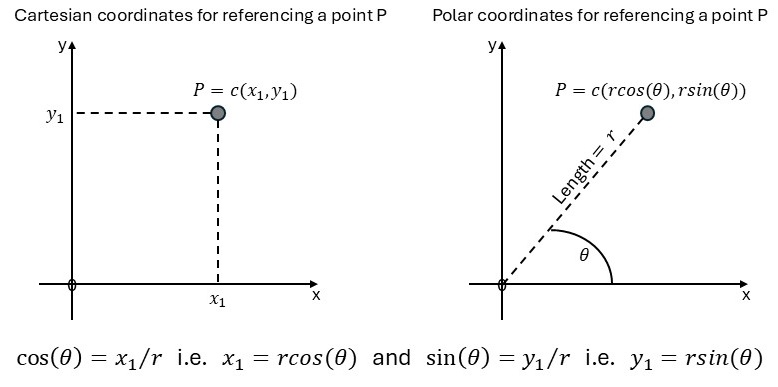
\includegraphics[width=1\linewidth]{pics/coordinates} \caption{Cartesian and polar coordinates for referencing a point on a graph.}\label{fig:coordinates}
\end{figure}

\begin{enumerate}
\def\labelenumi{(\roman{enumi})}
\tightlist
\item
  Consider the following function for drawing a circle with a specified radius and centred at the origin:
\end{enumerate}

\begin{Shaded}
\begin{Highlighting}[]
\NormalTok{my.circle }\OtherTok{\textless{}{-}} \ControlFlowTok{function}\NormalTok{ (}\AttributeTok{r =} \DecValTok{1}\NormalTok{, }\AttributeTok{xrange =} \SpecialCharTok{{-}}\DecValTok{2}\SpecialCharTok{:}\DecValTok{2}\NormalTok{, }\AttributeTok{yrange =} \SpecialCharTok{{-}}\DecValTok{2}\SpecialCharTok{:}\DecValTok{2}\NormalTok{) }
\NormalTok{\{ }\FunctionTok{plot}\NormalTok{ (}\AttributeTok{x =}\NormalTok{ xrange, }\AttributeTok{y =}\NormalTok{ yrange, }\AttributeTok{type =} \StringTok{\textquotesingle{}n\textquotesingle{}}\NormalTok{, }\AttributeTok{xlab =} \StringTok{\textquotesingle{}\textquotesingle{}}\NormalTok{, }\AttributeTok{ylab =} \StringTok{\textquotesingle{}\textquotesingle{}}\NormalTok{,}
        \AttributeTok{xaxt =} \StringTok{\textquotesingle{}n\textquotesingle{}}\NormalTok{, }\AttributeTok{yaxt =} \StringTok{\textquotesingle{}n\textquotesingle{}}\NormalTok{)}
\NormalTok{  theta }\OtherTok{\textless{}{-}} \FunctionTok{seq}\NormalTok{(}\AttributeTok{from =} \DecValTok{0}\NormalTok{, }\AttributeTok{to =} \DecValTok{2} \SpecialCharTok{*}\NormalTok{ pi, }\AttributeTok{by =} \FloatTok{0.01}\NormalTok{) }
  \CommentTok{\# Notice the use of radians.}
  \FunctionTok{lines}\NormalTok{ (}\AttributeTok{x =}\NormalTok{ r}\SpecialCharTok{*}\FunctionTok{cos}\NormalTok{(theta), }\AttributeTok{y =}\NormalTok{ r}\SpecialCharTok{*}\FunctionTok{sin}\NormalTok{(theta))}
  \FunctionTok{abline}\NormalTok{(}\AttributeTok{h =} \DecValTok{0}\NormalTok{)}
  \FunctionTok{abline}\NormalTok{(}\AttributeTok{v =} \DecValTok{0}\NormalTok{)}
\NormalTok{\}}
\end{Highlighting}
\end{Shaded}

Run the above function and consider the graph window. Increase and decrease the size of the graph window by dragging its edges. Does the figure look like a circle?

\begin{enumerate}
\def\labelenumi{(\roman{enumi})}
\setcounter{enumi}{1}
\item
  Next, add the argument \texttt{asp\ =\ 1} to the call to \texttt{plot} in \texttt{my.circle}. Run the changed function; change the size of the graph window. What happens?
\item
  What changes are necessary for producing a circle centred at any point in a geometrical space? Make the necessary changes in \texttt{my.circle()} for constructing a circle centred at any user specified point on a graph.
\end{enumerate}

\begin{enumerate}
\def\labelenumi{\arabic{enumi}.}
\setcounter{enumi}{10}
\item
  What is understood by a p-dimensional ellipsoid?

  \begin{enumerate}
  \def\labelenumii{(\roman{enumii})}
  \item
    Give a mathematical expression in matrix notation that describes an ellipsoid in p dimensions.
  \item
    Describe the axes of the ellipsoid in terms of eigenvalues and eigenvectors.
  \item
    Let \(p = 2\). Simplify the expression for the ellipse concerned in terms of scalar quantities.
  \item
    Use \texttt{plot()} and write an R-function to draw an ellipse. Make provision for the centre point to be at \((0, 0)\) as well as at an arbitrary \((x_1,x_2)\) point; for no correlation between the two variables as well as for positive and negative correlation.
  \item
    Use your function written in (iv) to illustrate differences between plot (using the default value of argument \texttt{asp}) and plot with \texttt{asp=1}.
  \end{enumerate}
\item
  During experimental design it is often useful to predict the value of the dependent variable at every combination of the levels of the factor variables. Write an R function for this task that makes provision for any number of factor arguments and that also provides a dataframe with the factors as the columns and every combination of levels as the rows. Every levels-combination can only appear once. The function must be user friendly and must test if a given independent variable is a factor variable. \emph{Hint}: Study the help file of \texttt{expand.grid()}.
\item
  Consider the following game. You are given a computer screen containing a rectangle filled at random with evenly spaced letters. Repetitions of the same letter are allowed. The challenge to the user is to sequentially select the first \(n\) letters of the alphabet as quickly as possible. The user must read each line from left to right and from top to bottom. Going backwards is not allowed. The time to complete the task is taken as well as whether the rules have been obeyed. Program an R version of this game.
\end{enumerate}

\chapter{Writing functions in R}\label{functions}

Although we have already written various functions in R, in this chapter the writing of R functions will be approached systematically.

\section{General}\label{general-2}

A good way to learn about functions or to write a new function is to look at existing ones. As an example consider that we would like to write a function to implement a novel plotting procedure. So we start by taking a look at the existing \texttt{plot} function.

\begin{Shaded}
\begin{Highlighting}[]
\NormalTok{plot}
\CommentTok{\#\textgreater{} function (x, y, ...) }
\CommentTok{\#\textgreater{} UseMethod("plot")}
\CommentTok{\#\textgreater{} \textless{}bytecode: 0x000002039c1332c8\textgreater{}}
\CommentTok{\#\textgreater{} \textless{}environment: namespace:base\textgreater{}}
\end{Highlighting}
\end{Shaded}

This is not very helpful so we give the instruction:

\begin{Shaded}
\begin{Highlighting}[]
\FunctionTok{methods}\NormalTok{(plot)}
\CommentTok{\#\textgreater{}  [1] plot.acf*           plot.data.frame*   }
\CommentTok{\#\textgreater{}  [3] plot.decomposed.ts* plot.default       }
\CommentTok{\#\textgreater{}  [5] plot.dendrogram*    plot.density*      }
\CommentTok{\#\textgreater{}  [7] plot.ecdf           plot.factor*       }
\CommentTok{\#\textgreater{}  [9] plot.formula*       plot.function      }
\CommentTok{\#\textgreater{} [11] plot.hclust*        plot.histogram*    }
\CommentTok{\#\textgreater{} [13] plot.HoltWinters*   plot.isoreg*       }
\CommentTok{\#\textgreater{} [15] plot.lm*            plot.medpolish*    }
\CommentTok{\#\textgreater{} [17] plot.mlm*           plot.ppr*          }
\CommentTok{\#\textgreater{} [19] plot.prcomp*        plot.princomp*     }
\CommentTok{\#\textgreater{} [21] plot.profile*       plot.profile.nls*  }
\CommentTok{\#\textgreater{} [23] plot.raster*        plot.spec*         }
\CommentTok{\#\textgreater{} [25] plot.stepfun        plot.stl*          }
\CommentTok{\#\textgreater{} [27] plot.table*         plot.ts            }
\CommentTok{\#\textgreater{} [29] plot.tskernel*      plot.TukeyHSD*     }
\CommentTok{\#\textgreater{} see \textquotesingle{}?methods\textquotesingle{} for accessing help and source code}
\end{Highlighting}
\end{Shaded}

If we decide to take a look at \texttt{plot.default} we can do so by

\begin{Shaded}
\begin{Highlighting}[]
\NormalTok{plot.default}
\CommentTok{\#\textgreater{} function (x, y = NULL, type = "p", xlim = NULL, ylim = NULL, }
\CommentTok{\#\textgreater{}     log = "", main = NULL, sub = NULL, xlab = NULL, ylab = NULL, }
\CommentTok{\#\textgreater{}     ann = par("ann"), axes = TRUE, frame.plot = axes, panel.first = NULL, }
\CommentTok{\#\textgreater{}     panel.last = NULL, asp = NA, xgap.axis = NA, ygap.axis = NA, }
\CommentTok{\#\textgreater{}     ...) }
\CommentTok{\#\textgreater{} \{}
\CommentTok{\#\textgreater{}     localAxis \textless{}{-} function(..., col, bg, pch, cex, lty, lwd) Axis(...)}
\CommentTok{\#\textgreater{}     localBox \textless{}{-} function(..., col, bg, pch, cex, lty, lwd) box(...)}
\CommentTok{\#\textgreater{}     localWindow \textless{}{-} function(..., col, bg, pch, cex, lty, lwd) plot.window(...)}
\CommentTok{\#\textgreater{}     localTitle \textless{}{-} function(..., col, bg, pch, cex, lty, lwd) title(...)}
\CommentTok{\#\textgreater{}     xlabel \textless{}{-} if (!missing(x)) }
\CommentTok{\#\textgreater{}         deparse1(substitute(x))}
\CommentTok{\#\textgreater{}     ylabel \textless{}{-} if (!missing(y)) }
\CommentTok{\#\textgreater{}         deparse1(substitute(y))}
\CommentTok{\#\textgreater{}     xy \textless{}{-} xy.coords(x, y, xlabel, ylabel, log)}
\CommentTok{\#\textgreater{}     if (is.null(xlab)) }
\CommentTok{\#\textgreater{}         xlab \textless{}{-} xy$xlab}
\CommentTok{\#\textgreater{}     if (is.null(ylab)) }
\CommentTok{\#\textgreater{}         ylab \textless{}{-} xy$ylab}
\CommentTok{\#\textgreater{}     if (is.null(xlim)) }
\CommentTok{\#\textgreater{}         xlim \textless{}{-} range(xy$x[is.finite(xy$x)])}
\CommentTok{\#\textgreater{}     if (is.null(ylim)) }
\CommentTok{\#\textgreater{}         ylim \textless{}{-} range(xy$y[is.finite(xy$y)])}
\CommentTok{\#\textgreater{}     dev.hold()}
\CommentTok{\#\textgreater{}     on.exit(dev.flush())}
\CommentTok{\#\textgreater{}     plot.new()}
\CommentTok{\#\textgreater{}     localWindow(xlim, ylim, log, asp, ...)}
\CommentTok{\#\textgreater{}     panel.first}
\CommentTok{\#\textgreater{}     plot.xy(xy, type, ...)}
\CommentTok{\#\textgreater{}     panel.last}
\CommentTok{\#\textgreater{}     if (axes) \{}
\CommentTok{\#\textgreater{}         localAxis(if (is.null(y)) }
\CommentTok{\#\textgreater{}             xy$x}
\CommentTok{\#\textgreater{}         else x, side = 1, gap.axis = xgap.axis, ...)}
\CommentTok{\#\textgreater{}         localAxis(if (is.null(y)) }
\CommentTok{\#\textgreater{}             x}
\CommentTok{\#\textgreater{}         else y, side = 2, gap.axis = ygap.axis, ...)}
\CommentTok{\#\textgreater{}     \}}
\CommentTok{\#\textgreater{}     if (frame.plot) }
\CommentTok{\#\textgreater{}         localBox(...)}
\CommentTok{\#\textgreater{}     if (ann) }
\CommentTok{\#\textgreater{}         localTitle(main = main, sub = sub, xlab = xlab, ylab = ylab, }
\CommentTok{\#\textgreater{}             ...)}
\CommentTok{\#\textgreater{}     invisible()}
\CommentTok{\#\textgreater{} \}}
\CommentTok{\#\textgreater{} \textless{}bytecode: 0x000002039cb3f028\textgreater{}}
\CommentTok{\#\textgreater{} \textless{}environment: namespace:graphics\textgreater{}}
\end{Highlighting}
\end{Shaded}

Since our new plotting method is aimed at categorical data we decide rather to take a look at \texttt{plot.factor}. But this is an asterisked function and hence is not visible:

\begin{Shaded}
\begin{Highlighting}[]
\NormalTok{plot.factor}
\CommentTok{\#\textgreater{} Error: object \textquotesingle{}plot.factor\textquotesingle{} not found}
\end{Highlighting}
\end{Shaded}

Asterisked functions can be inspected using the following method:

\begin{Shaded}
\begin{Highlighting}[]
\FunctionTok{getAnywhere}\NormalTok{(plot.factor)}
\CommentTok{\#\textgreater{} A single object matching \textquotesingle{}plot.factor\textquotesingle{} was found}
\CommentTok{\#\textgreater{} It was found in the following places}
\CommentTok{\#\textgreater{}   registered S3 method for plot from namespace graphics}
\CommentTok{\#\textgreater{}   namespace:graphics}
\CommentTok{\#\textgreater{} with value}
\CommentTok{\#\textgreater{} }
\CommentTok{\#\textgreater{} function (x, y, legend.text = NULL, ...) }
\CommentTok{\#\textgreater{} \{}
\CommentTok{\#\textgreater{}     if (missing(y) || is.factor(y)) \{}
\CommentTok{\#\textgreater{}         dargs \textless{}{-} list(...)}
\CommentTok{\#\textgreater{}         axisnames \textless{}{-} dargs$axes \%||\% if (!is.null(dargs$xaxt)) }
\CommentTok{\#\textgreater{}             dargs$xaxt != "n"}
\CommentTok{\#\textgreater{}         else TRUE}
\CommentTok{\#\textgreater{}     \}}
\CommentTok{\#\textgreater{}     if (missing(y)) \{}
\CommentTok{\#\textgreater{}         barplot(table(x), axisnames = axisnames, ...)}
\CommentTok{\#\textgreater{}     \}}
\CommentTok{\#\textgreater{}     else if (is.factor(y)) \{}
\CommentTok{\#\textgreater{}         if (is.null(legend.text)) }
\CommentTok{\#\textgreater{}             spineplot(x, y, ...)}
\CommentTok{\#\textgreater{}         else \{}
\CommentTok{\#\textgreater{}             args \textless{}{-} c(list(x = x, y = y), list(...))}
\CommentTok{\#\textgreater{}             args$yaxlabels \textless{}{-} legend.text}
\CommentTok{\#\textgreater{}             do.call("spineplot", args)}
\CommentTok{\#\textgreater{}         \}}
\CommentTok{\#\textgreater{}     \}}
\CommentTok{\#\textgreater{}     else if (is.numeric(y)) }
\CommentTok{\#\textgreater{}         boxplot(y \textasciitilde{} x, ...)}
\CommentTok{\#\textgreater{}     else NextMethod("plot")}
\CommentTok{\#\textgreater{} \}}
\CommentTok{\#\textgreater{} \textless{}bytecode: 0x000002039bd9f3e0\textgreater{}}
\CommentTok{\#\textgreater{} \textless{}environment: namespace:graphics\textgreater{}}
\end{Highlighting}
\end{Shaded}

\begin{enumerate}
\def\labelenumi{(\alph{enumi})}
\item
  How are default values assigned to arguments of functions?
\item
  What is the default behaviour of \texttt{plot.factor()}?
\item
  What tasks can be achieved with \texttt{pmatch()} and what is understood by partial matching? What will happen if \texttt{plot.factor()} is called with (i) \texttt{legend.text\ =\ \textquotesingle{}AA=Agecat\textquotesingle{}}; (ii) \texttt{leg\ =\ \textquotesingle{}AA=Agecat\textquotesingle{}}? Explain.
\item
  Discuss the usage of \texttt{missing()}.
\item
  Give an example of the usage of the function \texttt{stop(message=\ "\ ")}.
\item
  Give an example of the usage of the function \texttt{warning(message=\ "\ ")}.
\item
  What is the usage of the function \texttt{warnings()}?
\item
  Why can functions be called without specifying any arguments e.g.~\texttt{q()}?
\item
  If the body of a function consists only of a single instruction it is not necessary to enclose it with braces.
\item
  The convention is to use the last evaluated statement as a function's return value. If several objects are to be returned gather them in a list.
\item
  The function \texttt{return()} with a single object or a list of objects is useful to interrupt a function at some intermediate stage and return an object or a list of objects at that particular stage. This is usually done when a function is under development.
\item
  Sometimes there is no meaningful value to return e.g.~when a function is written primarily to produce some plot. In cases like this the function \texttt{invisible()} can be used as the last statement of the function. As an example of the usage of \texttt{invisible()} give the following instructions:
\end{enumerate}

\begin{Shaded}
\begin{Highlighting}[]
\FunctionTok{boxplot}\NormalTok{(}\FunctionTok{rnorm}\NormalTok{(}\DecValTok{100}\NormalTok{), }\AttributeTok{plot =} \ConstantTok{TRUE}\NormalTok{)}
\end{Highlighting}
\end{Shaded}

\pandocbounded{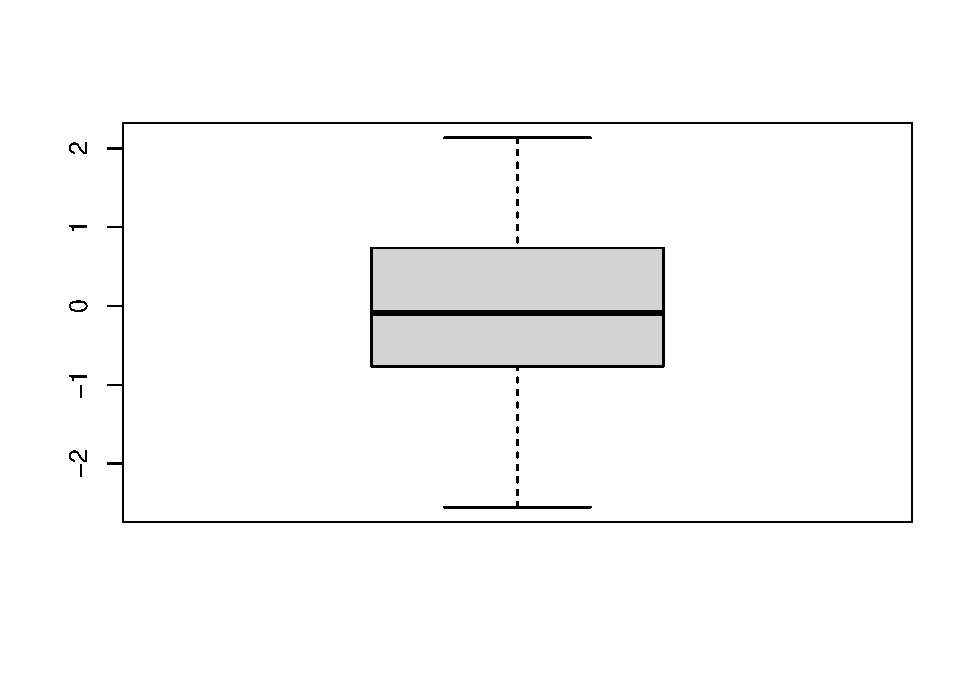
\includegraphics[keepaspectratio]{07-functions_files/figure-latex/invisibleExamples-1.pdf}}

\begin{Shaded}
\begin{Highlighting}[]
\FunctionTok{boxplot}\NormalTok{(}\FunctionTok{rnorm}\NormalTok{(}\DecValTok{100}\NormalTok{), }\AttributeTok{plot =} \ConstantTok{FALSE}\NormalTok{)}
\CommentTok{\#\textgreater{} $stats}
\CommentTok{\#\textgreater{}             [,1]}
\CommentTok{\#\textgreater{} [1,] {-}2.13673866}
\CommentTok{\#\textgreater{} [2,] {-}0.47854052}
\CommentTok{\#\textgreater{} [3,]  0.07906728}
\CommentTok{\#\textgreater{} [4,]  0.79507583}
\CommentTok{\#\textgreater{} [5,]  2.08596468}
\CommentTok{\#\textgreater{} }
\CommentTok{\#\textgreater{} $n}
\CommentTok{\#\textgreater{} [1] 100}
\CommentTok{\#\textgreater{} }
\CommentTok{\#\textgreater{} $conf}
\CommentTok{\#\textgreater{}            [,1]}
\CommentTok{\#\textgreater{} [1,] {-}0.1221641}
\CommentTok{\#\textgreater{} [2,]  0.2802987}
\CommentTok{\#\textgreater{} }
\CommentTok{\#\textgreater{} $out}
\CommentTok{\#\textgreater{} [1]  3.271010 {-}2.674717}
\CommentTok{\#\textgreater{} }
\CommentTok{\#\textgreater{} $group}
\CommentTok{\#\textgreater{} [1] 1 1}
\CommentTok{\#\textgreater{} }
\CommentTok{\#\textgreater{} $names}
\CommentTok{\#\textgreater{} [1] "1"}
\end{Highlighting}
\end{Shaded}

Now look at the end of function \texttt{boxplot.default()} to see how \texttt{invisible()} has been implemented.

\begin{enumerate}
\def\labelenumi{(\alph{enumi})}
\setcounter{enumi}{12}
\item
  Libraries (packages) of R functions. Attaching and detaching libraries to the search path. (Revise Chapter \ref{intro})
\item
  Creating a new function using scripts or \texttt{fix()}. (Revise Chapter \ref{intro})
\item
  Editing an existing function using scripts or \texttt{fix()}. (Revise Chapter \ref{intro})
\item
  Note that when writing a function a line can be interrupted at any place and be continued on a next line. \emph{{Warning: Be careful not to put the break point where it marks the completion of an executable statement.}} Explain.
\end{enumerate}

\section{Writing a new function}\label{writing-a-new-function}

Determining the indices of elements in a vector or matrix that meet a certain condition: the function \texttt{where()}

\begin{enumerate}
\def\labelenumi{(\alph{enumi})}
\tightlist
\item
  Write the following function:
\end{enumerate}

\begin{Shaded}
\begin{Highlighting}[]
\NormalTok{where }\OtherTok{\textless{}{-}} \ControlFlowTok{function}\NormalTok{(x, cond)}
\NormalTok{\{ }\CommentTok{\# Argument cond must evaluate to a logical value}
     \ControlFlowTok{if}\NormalTok{(}\SpecialCharTok{!}\FunctionTok{is.matrix}\NormalTok{(x))}
       \FunctionTok{seq}\NormalTok{(}\AttributeTok{along =}\NormalTok{ x)[cond]}
     \ControlFlowTok{else} \FunctionTok{matrix}\NormalTok{(}\FunctionTok{c}\NormalTok{(}\FunctionTok{row}\NormalTok{(x)[cond], }\FunctionTok{col}\NormalTok{(x)[cond]), }\AttributeTok{ncol =} \DecValTok{2}\NormalTok{)}
\NormalTok{\}}
\end{Highlighting}
\end{Shaded}

\begin{enumerate}
\def\labelenumi{(\alph{enumi})}
\setcounter{enumi}{1}
\item
  Inspect the \emph{airquality} data set using the command \texttt{str(airquality)}.
\item
  Use the \texttt{where()} function to find the indices of (i) the \texttt{NA}s, (ii) the maximum value and (iii) the minimum value in the airquality data set.
\item
  Repeat (b) using the built-in function \texttt{which()}.
\end{enumerate}

\section{Checking for object name clashes}\label{checking-for-object-name-clashes}

\begin{enumerate}
\def\labelenumi{(\alph{enumi})}
\item
  What happens if an R object is given the same name as an existing object?
\item
  Discuss the usages of the functions \texttt{apropos()}, \texttt{conflicts()}, \texttt{find()} and \texttt{match()} for the naming of objects.
\item
  Remember that when a function is called the R evaluator first looks in the \emph{{global environment}} for a function with this name and subsequently in each of the attached packages or date bases in the order shown by \texttt{search()}. The evaluator generally stops searching when the name is found for the first time. If two attached packages have functions with the same name one of them will \emph{{mask}} the object in the other. For example, the function \texttt{gam()} exists in two packages: \texttt{gam} and \texttt{mgcv}. If both were attached the command
\end{enumerate}

\begin{Shaded}
\begin{Highlighting}[]
\FunctionTok{library}\NormalTok{ (mgcv)}
\CommentTok{\#\textgreater{} Loading required package: nlme}
\CommentTok{\#\textgreater{} This is mgcv 1.9{-}3. For overview type \textquotesingle{}help("mgcv{-}package")\textquotesingle{}.}
\FunctionTok{library}\NormalTok{ (gam)}
\CommentTok{\#\textgreater{} Loading required package: splines}
\CommentTok{\#\textgreater{} Loading required package: foreach}
\CommentTok{\#\textgreater{} Loaded gam 1.22{-}6}
\CommentTok{\#\textgreater{} }
\CommentTok{\#\textgreater{} Attaching package: \textquotesingle{}gam\textquotesingle{}}
\CommentTok{\#\textgreater{} The following objects are masked from \textquotesingle{}package:mgcv\textquotesingle{}:}
\CommentTok{\#\textgreater{} }
\CommentTok{\#\textgreater{}     gam, gam.control, gam.fit, s}
\FunctionTok{find}\NormalTok{(}\StringTok{"gam"}\NormalTok{)}
\CommentTok{\#\textgreater{} [1] "package:gam"  "package:mgcv"}
\end{Highlighting}
\end{Shaded}

will return both version.

\begin{enumerate}
\def\labelenumi{(\alph{enumi})}
\setcounter{enumi}{3}
\item
  The operator \texttt{::} can be used to access the intended version of \texttt{gam()} by using the call \texttt{mgcv::gam()} or \texttt{gam::gam()}.
\item
  When writing R packages the \emph{{namespace}} of the package provides another mechanism for ensuring that the correct version of a function is used. Note in this regard that the operator \texttt{:::} can be used to access objects that are not exported.
\end{enumerate}

\section{Returning multiple values}\label{returning-multiple-values}

\subsection{Exercise}\label{exercise-11}

Write an R function that returns the mean, median, variance, minimum, maximum and coefficient of variation of a numeric vector of sample data. The different components must be accessible by name. Test your function with the value of \texttt{rnorm(1000)}. \emph{Hint}: Use the construct \texttt{list\ (mean\ =\ ...,\ median\ =\ ...,\ ...)}.

\section{Local variables and evaluation environments}\label{local-variables-and-evaluation-environments}

\begin{enumerate}
\def\labelenumi{(\alph{enumi})}
\item
  Where is an object stored that is created by a script or \texttt{fix()}?
\item
  Where are local objects (objects that are created during the execution of a function) stored?
\item
  Explain how the \emph{{evaluation environment}} works.
\item
  What is understood by the \emph{{global environment}}?
\item
  Study the R help-file w.r.t. the operator \texttt{\textless{}\textless{}-}. When is it useful to use this operator? What are the dangers inherent to this operator?
\item
  What is understood by the scope of an expression or function?
\end{enumerate}

The symbols which occur in the body of a function can be divided into three classes: \emph{{formal parameters}}, \emph{{local variables}} and \emph{{free variables}}. The formal parameters of a function are those appearing within the parentheses denoting the argument list of the function. Their values are determined by the process of \emph{{binding}} the actual function arguments to the formal parameters. Local variables are created by the evaluation of expressions in the body of the functions. Variables which are neither formal parameters nor local variables are called free variables. Free variables become local variables when they are assigned to. Consider the following function definition.

\begin{Shaded}
\begin{Highlighting}[]
\NormalTok{fun }\OtherTok{\textless{}{-}} \ControlFlowTok{function}\NormalTok{(datvec) \{}
\NormalTok{          mean }\OtherTok{\textless{}{-}} \FunctionTok{mean}\NormalTok{(datvec)}
          \FunctionTok{print}\NormalTok{(mean)}
          \FunctionTok{plot}\NormalTok{(datvec)}
          \FunctionTok{plot}\NormalTok{(Traffic)}
\NormalTok{       \}}
\end{Highlighting}
\end{Shaded}

In this function, \texttt{datvec} is a formal parameter, the object \texttt{mean} on the left-hand of the assignment symbol is a local variable (not to be confused with the function \texttt{mean()} on the right-hand side of the assignment symbol) while \texttt{Traffic} is a free variable. In R the free variable bindings are resolved by first looking in the \emph{{environment}} in which the function was created. This is called \emph{{lexical scope}}.

If the following function call is made from the prompt in the working directory \texttt{fun(1:25)} the formal parameter \texttt{datvec} within the body of the function is assigned the value \texttt{1:25} (the actual argument) and its mean is assigned to the local object \texttt{mean}. If the free parameter \texttt{Traffic} is found in the \emph{{global environment}} or in a data base on the search path the required graph will be created else an error message will be sent to the console. Perform the above call.

\section{Cleaning up}\label{cleaning-up}

\begin{enumerate}
\def\labelenumi{(\alph{enumi})}
\item
  Study how the function \texttt{on.exit()} is used. This function can be used to reset options that are changed during an R-session back to their original values when the session is ended or a function terminates with an error message. It is also convenient for removal of temporary files.
\item
  Study the uses of the functions \texttt{.First()} and \texttt{.Last()}.
\item
  Write a function that automatically opens a graph window with a square plot region when an R-session is started.
\end{enumerate}

\section{\texorpdfstring{Variable number of arguments: argument \texttt{...}}{Variable number of arguments: argument ...}}\label{variable-number-of-arguments-argument-...}

\begin{enumerate}
\def\labelenumi{(\alph{enumi})}
\tightlist
\item
  Consider the following situation: You want to write a function for a complex task. At a particular stage a graph of some intermediate results is to be constructed. This requires the calling function to contain a call to the \texttt{hist()} function. Here is an example of a chunk of code for executing this task:
\end{enumerate}

\begin{Shaded}
\begin{Highlighting}[]
\NormalTok{complexfun }\OtherTok{\textless{}{-}} \ControlFlowTok{function}\NormalTok{(datmat,colgraph)}
\NormalTok{    \{ datmat }\OtherTok{\textless{}{-}} \FunctionTok{scale}\NormalTok{(datmat) }
       \CommentTok{\# Several lines of complex code here }
      \FunctionTok{hist}\NormalTok{(datmat, }\AttributeTok{col =}\NormalTok{ colgraph)              \}}
\end{Highlighting}
\end{Shaded}

A call like \texttt{complexfun(rnorm(1000),\ \textquotesingle{}yellow\textquotesingle{})} can now be executed for the desired result. The problem is that the hist function has several arguments that you would like to be able to access by passing suitable actual values to them through the calling function \texttt{complexfun}. Instead of having to resort to provide a complete set of arguments in the argument list of \texttt{complexfun} R provides a neat way of addressing this situation: The argument \texttt{...} which acts like any other formal argument except that it can represent a variable number of arguments. To see how the argument \texttt{...} works change the above function to:

\begin{Shaded}
\begin{Highlighting}[]
\NormalTok{complexfun2 }\OtherTok{\textless{}{-}} \ControlFlowTok{function}\NormalTok{(datmat, ... )}
\NormalTok{ \{ datmat }\OtherTok{\textless{}{-}} \FunctionTok{scale}\NormalTok{(datmat) }
       \CommentTok{\# Several lines of complex code here }
   \FunctionTok{hist}\NormalTok{(datmat, ... )    \}}
\end{Highlighting}
\end{Shaded}

Arguments represented by argument \texttt{...} in the argument list of hist are passed to hist through the argument \texttt{...} appearing in the arguments list of function \texttt{complexfun2}:

\begin{Shaded}
\begin{Highlighting}[]
\FunctionTok{complexfun2}\NormalTok{(}\AttributeTok{datmat =} \FunctionTok{rnorm}\NormalTok{(}\DecValTok{1000}\NormalTok{), }\AttributeTok{col =} \StringTok{\textquotesingle{}yellow\textquotesingle{}}\NormalTok{, }
        \AttributeTok{probability =} \ConstantTok{TRUE}\NormalTok{, }\AttributeTok{xlim =} \FunctionTok{c}\NormalTok{(}\SpecialCharTok{{-}}\DecValTok{5}\NormalTok{,}\DecValTok{5}\NormalTok{))}
\end{Highlighting}
\end{Shaded}

\begin{enumerate}
\def\labelenumi{(\alph{enumi})}
\setcounter{enumi}{1}
\tightlist
\item
  Write a function that will retrieve the maximum length of any of an unspecified number of arguments of a specified mode. This is another example of the use of the \texttt{...} argument:
\end{enumerate}

\begin{Shaded}
\begin{Highlighting}[]
\NormalTok{maxlen }\OtherTok{\textless{}{-}} \ControlFlowTok{function}\NormalTok{ (}\AttributeTok{mode.use=}\StringTok{"numeric"}\NormalTok{, ...) }
\NormalTok{  \{ my.list }\OtherTok{\textless{}{-}} \FunctionTok{list}\NormalTok{(...)}
\NormalTok{    out }\OtherTok{\textless{}{-}} \DecValTok{0}
    \ControlFlowTok{for}\NormalTok{(x }\ControlFlowTok{in}\NormalTok{ my.list) }
      \FunctionTok{print}\NormalTok{ (}\FunctionTok{mode}\NormalTok{(x)) }\CommentTok{\#if(mode(x) == mode.use) out \textless{}{-} max(out,length(x))}
\NormalTok{    out}
\NormalTok{  \}}
\end{Highlighting}
\end{Shaded}

Note that the named argument must be specified as such in the function call:

\begin{Shaded}
\begin{Highlighting}[]
\FunctionTok{maxlen}\NormalTok{(}\DecValTok{1}\SpecialCharTok{:}\DecValTok{10}\NormalTok{, }\DecValTok{1}\SpecialCharTok{:}\DecValTok{15}\NormalTok{, }\DecValTok{1}\SpecialCharTok{:}\DecValTok{3}\NormalTok{, letters)}
\CommentTok{\#\textgreater{} [1] "numeric"}
\CommentTok{\#\textgreater{} [1] "numeric"}
\CommentTok{\#\textgreater{} [1] "character"}
\CommentTok{\#\textgreater{} [1] 0}
\FunctionTok{maxlen}\NormalTok{(}\AttributeTok{mode.use=}\StringTok{"numeric"}\NormalTok{, }\DecValTok{1}\SpecialCharTok{:}\DecValTok{10}\NormalTok{, }\DecValTok{1}\SpecialCharTok{:}\DecValTok{15}\NormalTok{, }\DecValTok{1}\SpecialCharTok{:}\DecValTok{3}\NormalTok{, letters)}
\CommentTok{\#\textgreater{} [1] "numeric"}
\CommentTok{\#\textgreater{} [1] "numeric"}
\CommentTok{\#\textgreater{} [1] "numeric"}
\CommentTok{\#\textgreater{} [1] "character"}
\CommentTok{\#\textgreater{} [1] 0}
\FunctionTok{maxlen}\NormalTok{(}\DecValTok{1}\SpecialCharTok{:}\DecValTok{10}\NormalTok{, }\DecValTok{1}\SpecialCharTok{:}\DecValTok{15}\NormalTok{, }\DecValTok{1}\SpecialCharTok{:}\DecValTok{3}\NormalTok{, letters, }\AttributeTok{mode.use=}\StringTok{"character"}\NormalTok{)}
\CommentTok{\#\textgreater{} [1] "numeric"}
\CommentTok{\#\textgreater{} [1] "numeric"}
\CommentTok{\#\textgreater{} [1] "numeric"}
\CommentTok{\#\textgreater{} [1] "character"}
\CommentTok{\#\textgreater{} [1] 0}
\FunctionTok{maxlen}\NormalTok{(}\AttributeTok{mode.use=}\StringTok{"character"}\NormalTok{, }\DecValTok{1}\SpecialCharTok{:}\DecValTok{10}\NormalTok{, }\DecValTok{1}\SpecialCharTok{:}\DecValTok{15}\NormalTok{, }\DecValTok{1}\SpecialCharTok{:}\DecValTok{3}\NormalTok{, letters)}
\CommentTok{\#\textgreater{} [1] "numeric"}
\CommentTok{\#\textgreater{} [1] "numeric"}
\CommentTok{\#\textgreater{} [1] "numeric"}
\CommentTok{\#\textgreater{} [1] "character"}
\CommentTok{\#\textgreater{} [1] 0}
\end{Highlighting}
\end{Shaded}

\section{\texorpdfstring{Retrieving names of arguments: functions \texttt{deparse()} and \texttt{substitute()}}{Retrieving names of arguments: functions deparse() and substitute()}}\label{retrieving-names-of-arguments-functions-deparse-and-substitute}

There are many practical situations requiring the conversion of mathematical expressions into character strings (text) or, conversely, requiring the conversion of text into mathematical expressions. The tools (functions) provided in R for achieving such conversions are summarized in Figure \ref{fig:expression}.

\begin{figure}
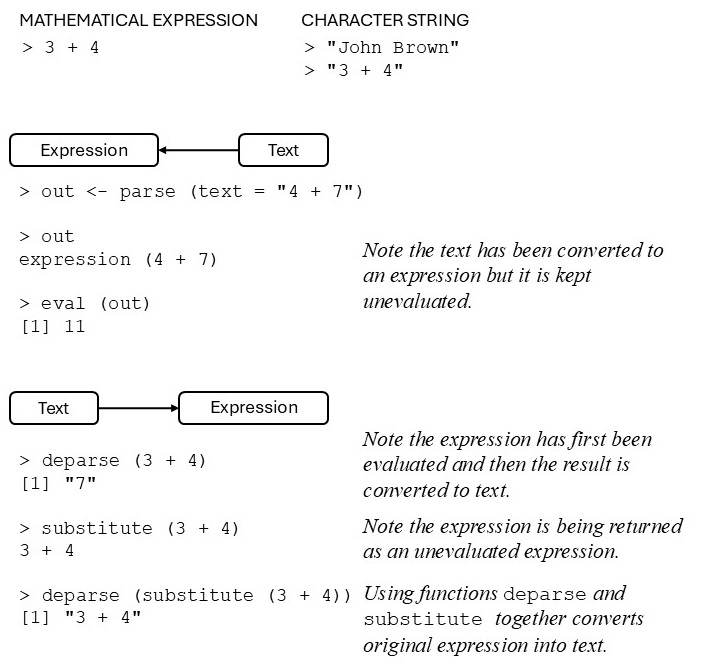
\includegraphics[width=0.8\linewidth]{pics/expressions} \caption{Converting text into mathematical expression or mathematical expressions into text.}\label{fig:expression}
\end{figure}

\begin{itemize}
\tightlist
\item
  Task: write an R function that will plot two vectors using as axis labels the names of the objects passed as arguments to the function.
\end{itemize}

It follows from Figure \ref{fig:expression} that the function \texttt{substitute()} takes an expression as argument and returns it unevaluated. In order to evaluate the return value of \texttt{substitute()} the function \texttt{eval()} must be used. The function \texttt{deparse()} takes as argument an unevaluated expression and converts it into a character string. Now we are ready to write the following function:

\begin{Shaded}
\begin{Highlighting}[]
\NormalTok{labplot }\OtherTok{\textless{}{-}} \ControlFlowTok{function}\NormalTok{ (x,y) }
\NormalTok{\{ xname }\OtherTok{\textless{}{-}} \FunctionTok{deparse}\NormalTok{(}\FunctionTok{substitute}\NormalTok{(x))}
\NormalTok{ yname }\OtherTok{\textless{}{-}} \FunctionTok{deparse}\NormalTok{(}\FunctionTok{substitute}\NormalTok{(y))}
 \FunctionTok{plot}\NormalTok{(x,y, }\AttributeTok{xlab=}\NormalTok{xname, }\AttributeTok{ylab=}\NormalTok{yname, }\AttributeTok{main =} \FunctionTok{paste}\NormalTok{(}\StringTok{"Plot of"}\NormalTok{,}
\NormalTok{        yname,}\StringTok{"versus"}\NormalTok{, xname))}
\NormalTok{\}}
\end{Highlighting}
\end{Shaded}

\begin{enumerate}
\def\labelenumi{(\alph{enumi})}
\item
  Study and illustrate the usage of function \texttt{labplot()}.
\item
  From Figure \ref{fig:expression} it also follows that the function \texttt{parse()} does the opposite of \texttt{deparse()} by converting a character string into an unevaluated expression. The latter unevaluated expression can be evaluated when needed using \texttt{eval()}.
\end{enumerate}

\section{Operators}\label{operators-1}

Execute the following instruction

\begin{Shaded}
\begin{Highlighting}[]
\FunctionTok{objects}\NormalTok{(}\StringTok{\textquotesingle{}package:base\textquotesingle{}}\NormalTok{)[}\DecValTok{1}\SpecialCharTok{:}\DecValTok{31}\NormalTok{]}
\CommentTok{\#\textgreater{}  [1] "{-}"                 "{-}.Date"           }
\CommentTok{\#\textgreater{}  [3] "{-}.POSIXt"          "!"                }
\CommentTok{\#\textgreater{}  [5] "!.hexmode"         "!.octmode"        }
\CommentTok{\#\textgreater{}  [7] "!="                "$"                }
\CommentTok{\#\textgreater{}  [9] "$.DLLInfo"         "$.package\_version"}
\CommentTok{\#\textgreater{} [11] "$\textless{}{-}"               "$\textless{}{-}.data.frame"   }
\CommentTok{\#\textgreater{} [13] "$\textless{}{-}.POSIXlt"       "\%\%"               }
\CommentTok{\#\textgreater{} [15] "\%*\%"               "\%/\%"              }
\CommentTok{\#\textgreater{} [17] "\%||\%"              "\%in\%"             }
\CommentTok{\#\textgreater{} [19] "\%o\%"               "\%x\%"              }
\CommentTok{\#\textgreater{} [21] "\&"                 "\&\&"               }
\CommentTok{\#\textgreater{} [23] "\&.hexmode"         "\&.octmode"        }
\CommentTok{\#\textgreater{} [25] "("                 "*"                }
\CommentTok{\#\textgreater{} [27] "*.difftime"        "/"                }
\CommentTok{\#\textgreater{} [29] "/.difftime"        ":"                }
\CommentTok{\#\textgreater{} [31] "::"}
\end{Highlighting}
\end{Shaded}

in order to obtain some examples of operators available in R.

\begin{enumerate}
\def\labelenumi{(\alph{enumi})}
\tightlist
\item
  \emph{{Operators are special R functions.}} Discuss this statement. In what respects do operators differ from ordinary R functions?
\end{enumerate}

\begin{enumerate}
\def\labelenumi{(\alph{enumi})}
\setcounter{enumi}{1}
\tightlist
\item
  Write an operator \texttt{\%E\%} to determine the Euclidean distance between two vectors and give an example of its usage. \emph{Hint}: when creating operators with \texttt{fix()} or using scripts the name must be given as a character string e.g.~\texttt{fix("\%E\%")}.
\end{enumerate}

\section{Replacement functions}\label{replacement-functions}

Execute the following instruction

\begin{Shaded}
\begin{Highlighting}[]
\FunctionTok{objects}\NormalTok{(}\StringTok{\textquotesingle{}package:base\textquotesingle{}}\NormalTok{)[}\DecValTok{300}\SpecialCharTok{:}\DecValTok{400}\NormalTok{]}
\CommentTok{\#\textgreater{}   [1] "c.factor"                  }
\CommentTok{\#\textgreater{}   [2] "c.noquote"                 }
\CommentTok{\#\textgreater{}   [3] "c.numeric\_version"         }
\CommentTok{\#\textgreater{}   [4] "c.POSIXct"                 }
\CommentTok{\#\textgreater{}   [5] "c.POSIXlt"                 }
\CommentTok{\#\textgreater{}   [6] "c.warnings"                }
\CommentTok{\#\textgreater{}   [7] "call"                      }
\CommentTok{\#\textgreater{}   [8] "callCC"                    }
\CommentTok{\#\textgreater{}   [9] "capabilities"              }
\CommentTok{\#\textgreater{}  [10] "casefold"                  }
\CommentTok{\#\textgreater{}  [11] "cat"                       }
\CommentTok{\#\textgreater{}  [12] "cbind"                     }
\CommentTok{\#\textgreater{}  [13] "cbind.data.frame"          }
\CommentTok{\#\textgreater{}  [14] "ceiling"                   }
\CommentTok{\#\textgreater{}  [15] "char.expand"               }
\CommentTok{\#\textgreater{}  [16] "character"                 }
\CommentTok{\#\textgreater{}  [17] "charmatch"                 }
\CommentTok{\#\textgreater{}  [18] "charToRaw"                 }
\CommentTok{\#\textgreater{}  [19] "chartr"                    }
\CommentTok{\#\textgreater{}  [20] "chkDots"                   }
\CommentTok{\#\textgreater{}  [21] "chol"                      }
\CommentTok{\#\textgreater{}  [22] "chol.default"              }
\CommentTok{\#\textgreater{}  [23] "chol2inv"                  }
\CommentTok{\#\textgreater{}  [24] "choose"                    }
\CommentTok{\#\textgreater{}  [25] "chooseOpsMethod"           }
\CommentTok{\#\textgreater{}  [26] "chooseOpsMethod.default"   }
\CommentTok{\#\textgreater{}  [27] "class"                     }
\CommentTok{\#\textgreater{}  [28] "class\textless{}{-}"                   }
\CommentTok{\#\textgreater{}  [29] "clearPushBack"             }
\CommentTok{\#\textgreater{}  [30] "close"                     }
\CommentTok{\#\textgreater{}  [31] "close.connection"          }
\CommentTok{\#\textgreater{}  [32] "close.srcfile"             }
\CommentTok{\#\textgreater{}  [33] "close.srcfilealias"        }
\CommentTok{\#\textgreater{}  [34] "closeAllConnections"       }
\CommentTok{\#\textgreater{}  [35] "col"                       }
\CommentTok{\#\textgreater{}  [36] "colMeans"                  }
\CommentTok{\#\textgreater{}  [37] "colnames"                  }
\CommentTok{\#\textgreater{}  [38] "colnames\textless{}{-}"                }
\CommentTok{\#\textgreater{}  [39] "colSums"                   }
\CommentTok{\#\textgreater{}  [40] "commandArgs"               }
\CommentTok{\#\textgreater{}  [41] "comment"                   }
\CommentTok{\#\textgreater{}  [42] "comment\textless{}{-}"                 }
\CommentTok{\#\textgreater{}  [43] "complex"                   }
\CommentTok{\#\textgreater{}  [44] "computeRestarts"           }
\CommentTok{\#\textgreater{}  [45] "conditionCall"             }
\CommentTok{\#\textgreater{}  [46] "conditionCall.condition"   }
\CommentTok{\#\textgreater{}  [47] "conditionMessage"          }
\CommentTok{\#\textgreater{}  [48] "conditionMessage.condition"}
\CommentTok{\#\textgreater{}  [49] "conflictRules"             }
\CommentTok{\#\textgreater{}  [50] "conflicts"                 }
\CommentTok{\#\textgreater{}  [51] "Conj"                      }
\CommentTok{\#\textgreater{}  [52] "contributors"              }
\CommentTok{\#\textgreater{}  [53] "cos"                       }
\CommentTok{\#\textgreater{}  [54] "cosh"                      }
\CommentTok{\#\textgreater{}  [55] "cospi"                     }
\CommentTok{\#\textgreater{}  [56] "crossprod"                 }
\CommentTok{\#\textgreater{}  [57] "Cstack\_info"               }
\CommentTok{\#\textgreater{}  [58] "cummax"                    }
\CommentTok{\#\textgreater{}  [59] "cummin"                    }
\CommentTok{\#\textgreater{}  [60] "cumprod"                   }
\CommentTok{\#\textgreater{}  [61] "cumsum"                    }
\CommentTok{\#\textgreater{}  [62] "curlGetHeaders"            }
\CommentTok{\#\textgreater{}  [63] "cut"                       }
\CommentTok{\#\textgreater{}  [64] "cut.Date"                  }
\CommentTok{\#\textgreater{}  [65] "cut.default"               }
\CommentTok{\#\textgreater{}  [66] "cut.POSIXt"                }
\CommentTok{\#\textgreater{}  [67] "data.class"                }
\CommentTok{\#\textgreater{}  [68] "data.frame"                }
\CommentTok{\#\textgreater{}  [69] "data.matrix"               }
\CommentTok{\#\textgreater{}  [70] "date"                      }
\CommentTok{\#\textgreater{}  [71] "debug"                     }
\CommentTok{\#\textgreater{}  [72] "debuggingState"            }
\CommentTok{\#\textgreater{}  [73] "debugonce"                 }
\CommentTok{\#\textgreater{}  [74] "declare"                   }
\CommentTok{\#\textgreater{}  [75] "default.stringsAsFactors"  }
\CommentTok{\#\textgreater{}  [76] "delayedAssign"             }
\CommentTok{\#\textgreater{}  [77] "deparse"                   }
\CommentTok{\#\textgreater{}  [78] "deparse1"                  }
\CommentTok{\#\textgreater{}  [79] "det"                       }
\CommentTok{\#\textgreater{}  [80] "detach"                    }
\CommentTok{\#\textgreater{}  [81] "determinant"               }
\CommentTok{\#\textgreater{}  [82] "determinant.matrix"        }
\CommentTok{\#\textgreater{}  [83] "dget"                      }
\CommentTok{\#\textgreater{}  [84] "diag"                      }
\CommentTok{\#\textgreater{}  [85] "diag\textless{}{-}"                    }
\CommentTok{\#\textgreater{}  [86] "diff"                      }
\CommentTok{\#\textgreater{}  [87] "diff.Date"                 }
\CommentTok{\#\textgreater{}  [88] "diff.default"              }
\CommentTok{\#\textgreater{}  [89] "diff.difftime"             }
\CommentTok{\#\textgreater{}  [90] "diff.POSIXt"               }
\CommentTok{\#\textgreater{}  [91] "difftime"                  }
\CommentTok{\#\textgreater{}  [92] "digamma"                   }
\CommentTok{\#\textgreater{}  [93] "dim"                       }
\CommentTok{\#\textgreater{}  [94] "dim.data.frame"            }
\CommentTok{\#\textgreater{}  [95] "dim\textless{}{-}"                     }
\CommentTok{\#\textgreater{}  [96] "dimnames"                  }
\CommentTok{\#\textgreater{}  [97] "dimnames.data.frame"       }
\CommentTok{\#\textgreater{}  [98] "dimnames\textless{}{-}"                }
\CommentTok{\#\textgreater{}  [99] "dimnames\textless{}{-}.data.frame"     }
\CommentTok{\#\textgreater{} [100] "dir"                       }
\CommentTok{\#\textgreater{} [101] "dir.create"}
\end{Highlighting}
\end{Shaded}

and notice that some object names appear in pairs with the name of one member of the pair ending in \texttt{\textless{}-}. Examples are \texttt{dim\textless{}-}, \texttt{levels\textless{}-}, \texttt{diag\textless{}-}, \texttt{names\textless{}-}, \texttt{rownames\textless{}-}, \texttt{colnames\textless{}-} and \texttt{dimnames\textless{}-}. Functions having names ending in \texttt{\textless{}-} are called \emph{{replacement}} functions. A replacement function appears on the left-hand side of the assignment symbol using the name without the \texttt{\textless{}-} to replace contents of the objects appearing in its argument list by the contents of the object appearing at the right-hand side of the assignment symbol e.g.:

\begin{Shaded}
\begin{Highlighting}[]
\NormalTok{X }\OtherTok{\textless{}{-}} \FunctionTok{matrix}\NormalTok{ (}\DecValTok{1}\SpecialCharTok{:}\DecValTok{12}\NormalTok{, }\AttributeTok{ncol =} \DecValTok{3}\NormalTok{, }\AttributeTok{dimnames =} 
               \FunctionTok{list}\NormalTok{ (}\FunctionTok{paste0}\NormalTok{ (}\StringTok{"Row"}\NormalTok{, }\DecValTok{1}\SpecialCharTok{:}\DecValTok{4}\NormalTok{), }\FunctionTok{paste0}\NormalTok{ (}\StringTok{"X"}\NormalTok{, }\DecValTok{1}\SpecialCharTok{:}\DecValTok{3}\NormalTok{)))}
\NormalTok{a }\OtherTok{\textless{}{-}} \FunctionTok{rownames}\NormalTok{(X) }\CommentTok{\# Function rownames in action.}
\FunctionTok{rownames}\NormalTok{(X) }\OtherTok{\textless{}{-}} \DecValTok{1}\SpecialCharTok{:}\FunctionTok{nrow}\NormalTok{(X) }\CommentTok{\# Replacement function \textquotesingle{}rownames\textless{}{-}\textquotesingle{} in action.}
\end{Highlighting}
\end{Shaded}

How can the object \texttt{diag\textless{}-} be inspected and is it different from the object \texttt{diag}? Compare the result of the following function calls:

\begin{Shaded}
\begin{Highlighting}[]
\FunctionTok{getAnywhere}\NormalTok{(}\StringTok{\textquotesingle{}diag\textquotesingle{}}\NormalTok{)}
\CommentTok{\#\textgreater{} 2 differing objects matching \textquotesingle{}diag\textquotesingle{} were found}
\CommentTok{\#\textgreater{} in the following places}
\CommentTok{\#\textgreater{}   package:base}
\CommentTok{\#\textgreater{}   namespace:Matrix}
\CommentTok{\#\textgreater{}   namespace:base}
\CommentTok{\#\textgreater{} Use [] to view one of them}
\FunctionTok{getAnywhere}\NormalTok{(}\StringTok{\textquotesingle{}diag\textless{}{-}\textquotesingle{}}\NormalTok{)}
\CommentTok{\#\textgreater{} 2 differing objects matching \textquotesingle{}diag\textless{}{-}\textquotesingle{} were found}
\CommentTok{\#\textgreater{} in the following places}
\CommentTok{\#\textgreater{}   package:base}
\CommentTok{\#\textgreater{}   namespace:Matrix}
\CommentTok{\#\textgreater{}   namespace:base}
\CommentTok{\#\textgreater{} Use [] to view one of them}
\end{Highlighting}
\end{Shaded}

In what respects do replacement functions differ from other functions?

In order to write a replacement function the following rules must be met:

\begin{enumerate}
\def\labelenumi{(\roman{enumi})}
\item
  the function name must end in \texttt{\textless{}-}
\item
  the function must return the complete object with suitable changes made
\item
  the final argument of the function corresponding to the replacement data on the right-hand side of the assignment, must be named \texttt{value}
\item
  usually a companion function exists having the same name without the \texttt{\textless{}-}.
\end{enumerate}

As an example, write a replacement function \texttt{undefined()} that will replace missing values in a data object with the values on its right-hand side:

\begin{Shaded}
\begin{Highlighting}[]
\StringTok{"undefined\textless{}{-}"} \OtherTok{\textless{}{-}} \ControlFlowTok{function}\NormalTok{ (x, }\AttributeTok{codes =} \FunctionTok{numeric}\NormalTok{(), value) }
\NormalTok{  \{ }\ControlFlowTok{if}\NormalTok{ (}\FunctionTok{length}\NormalTok{(codes) }\SpecialCharTok{\textgreater{}} \DecValTok{0}\NormalTok{) x[x }\SpecialCharTok{\%in\%}\NormalTok{ codes] }\OtherTok{\textless{}{-}} \ConstantTok{NA}
\NormalTok{    x[}\FunctionTok{is.na}\NormalTok{(x)] }\OtherTok{\textless{}{-}}\NormalTok{ value}
\NormalTok{    x}
\NormalTok{  \}}
\end{Highlighting}
\end{Shaded}

The above function can be created or edited using \texttt{fix("undefined\textless{}-")}. Illustrate the usage of \texttt{undefined()}.

\section{Default values and lazy evaluation}\label{default-values-and-lazy-evaluation}

\begin{enumerate}
\def\labelenumi{(\alph{enumi})}
\tightlist
\item
  The function \texttt{match.arg()} is useful for selecting a default value from one of a set of possible values. Consider the following example:
\end{enumerate}

\begin{Shaded}
\begin{Highlighting}[]
\NormalTok{choice }\OtherTok{\textless{}{-}} \ControlFlowTok{function}\NormalTok{(}\AttributeTok{method=}\FunctionTok{c}\NormalTok{(}\StringTok{"PCA"}\NormalTok{,}\StringTok{"CVA"}\NormalTok{,}\StringTok{"CA"}\NormalTok{,}\StringTok{"NONLIN"}\NormalTok{))}
\NormalTok{   \{ }\FunctionTok{match.arg}\NormalTok{(method)  \}}
\FunctionTok{choice}\NormalTok{()}
\CommentTok{\#\textgreater{} [1] "PCA"}
\FunctionTok{choice}\NormalTok{(}\StringTok{"CVA"}\NormalTok{)}
\CommentTok{\#\textgreater{} [1] "CVA"}
\FunctionTok{choice}\NormalTok{(}\StringTok{"xx"}\NormalTok{)}
\CommentTok{\#\textgreater{} Error in match.arg(method): \textquotesingle{}arg\textquotesingle{} should be one of "PCA", "CVA", "CA", "NONLIN"}
\end{Highlighting}
\end{Shaded}

\begin{enumerate}
\def\labelenumi{(\alph{enumi})}
\setcounter{enumi}{1}
\tightlist
\item
  Functions in the R language are governed by a principle known as \emph{{lazy evaluation}} which means that a default value is not evaluated until it is actually needed within the function body. As a result of lazy evaluation it might happen in a function call that some default values are never evaluated.
\end{enumerate}

\section{The dynamic loading of external routines}\label{the-dynamic-loading-of-external-routines}

Compiled code can run in some instances much faster than corresponding code in R. The functions \texttt{.C()} and \texttt{.Fortran()} allow users to make use of programs written in \emph{{C}} or \emph{{Fortran}} in their R functions. How this is done is illustrated below. Study this example carefully and consult the help files for more details when needed.

First an R function is created to compute the matrix product of two matrices:

\begin{Shaded}
\begin{Highlighting}[]
\NormalTok{matmult }\OtherTok{\textless{}{-}} \ControlFlowTok{function}\NormalTok{ (A,B) }
\NormalTok{ \{ }\ControlFlowTok{if}\NormalTok{(}\FunctionTok{ncol}\NormalTok{(A) }\SpecialCharTok{!=} \FunctionTok{nrow}\NormalTok{(B)) }\FunctionTok{stop}\NormalTok{(}\StringTok{"A and B not conformable with                 }
\StringTok{                       respect to matrix multiplication }\SpecialCharTok{\textbackslash{}n}\StringTok{"}\NormalTok{)}
\NormalTok{   n }\OtherTok{\textless{}{-}} \FunctionTok{nrow}\NormalTok{(A)}
\NormalTok{   q }\OtherTok{\textless{}{-}} \FunctionTok{ncol}\NormalTok{(B)}
\NormalTok{   Cmat }\OtherTok{\textless{}{-}} \FunctionTok{matrix}\NormalTok{(}\ConstantTok{NA}\NormalTok{, }\AttributeTok{nrow=}\NormalTok{n, }\AttributeTok{ncol=}\NormalTok{q)}
   \ControlFlowTok{for}\NormalTok{(i }\ControlFlowTok{in} \DecValTok{1}\SpecialCharTok{:}\NormalTok{n)}
\NormalTok{      \{ }\ControlFlowTok{for}\NormalTok{(j }\ControlFlowTok{in} \DecValTok{1}\SpecialCharTok{:}\NormalTok{q) Cmat[i,j] }\OtherTok{\textless{}{-}} \FunctionTok{sum}\NormalTok{(A[i,] }\SpecialCharTok{*}\NormalTok{ B[,j])}
\NormalTok{      \}}
\NormalTok{  Cmat}
\NormalTok{  \}}
\end{Highlighting}
\end{Shaded}

Next a \emph{{Fortran}} subroutine is written for performing matrix multiplication. The \emph{{Fortran}} code for this subroutine is given below:

\begin{Shaded}
\begin{Highlighting}[]
\NormalTok{      SUBROUTINE MATM (A1, A2B1, B2, A, B, OUT)}
\NormalTok{C     This subroutine performs matrix multiplication.}
\NormalTok{C     This should be improved with optimized code (such as }
\NormalTok{C     from Linpack, etc.)}
\NormalTok{      IMPLICIT NONE}
\NormalTok{      INTEGER A1, A2B1, B2}
\NormalTok{      DOUBLE PRECISION A(A1,A2B1), B(A2B1,B2), OUT(A1,B2)}
\NormalTok{C     DUMMIES}
\NormalTok{      INTEGER I, J, K}
\NormalTok{      DO 300,J=1,B2}
\NormalTok{        DO 200,I=1,A1}
\NormalTok{          OUT(I,J)=0}
\NormalTok{          DO 100,K=1,A2B1}
\NormalTok{            OUT(I,J)=OUT(I,J)+A(I,K)*B(K,J)}
\NormalTok{100   CONTINUE}
\NormalTok{200   CONTINUE}
\NormalTok{300   CONTINUE}
\NormalTok{      END}
\end{Highlighting}
\end{Shaded}

Next a dynamic link library (\emph{{.dll}}) is made from the \emph{{Fortran}} subroutine. The easiest way to do this is to use the command \texttt{R\ CMD\ SHLIB\ matm.f} from the \emph{{Command Prompt}}. The \emph{{.dll}} is available as \emph{{C:\matm64.dll}}.

Now an R function is to be written where the \emph{{Fortran}} code is called:

\begin{Shaded}
\begin{Highlighting}[]
\NormalTok{matmult.Fortran }\OtherTok{\textless{}{-}}\ControlFlowTok{function}\NormalTok{ (A,B) }
\NormalTok{ \{ }\ControlFlowTok{if}\NormalTok{(}\FunctionTok{ncol}\NormalTok{(A) }\SpecialCharTok{!=} \FunctionTok{nrow}\NormalTok{(B)) }\FunctionTok{stop}\NormalTok{(}\StringTok{"A and B not conformable with }
\StringTok{                       respect to matrix multiplication }\SpecialCharTok{\textbackslash{}n}\StringTok{"}\NormalTok{)}
\NormalTok{    n }\OtherTok{\textless{}{-}} \FunctionTok{nrow}\NormalTok{(A)}
\NormalTok{    q }\OtherTok{\textless{}{-}} \FunctionTok{ncol}\NormalTok{(B)}
\NormalTok{    p }\OtherTok{\textless{}{-}} \FunctionTok{ncol}\NormalTok{(A)}
\NormalTok{    Cmat }\OtherTok{\textless{}{-}} \FunctionTok{matrix}\NormalTok{(}\DecValTok{0}\NormalTok{, }\AttributeTok{nrow=}\NormalTok{n, }\AttributeTok{ncol=}\NormalTok{q)}
    \FunctionTok{storage.mode}\NormalTok{(A) }\OtherTok{\textless{}{-}} \StringTok{"double"}
    \FunctionTok{storage.mode}\NormalTok{(B) }\OtherTok{\textless{}{-}} \StringTok{"double"}
    \FunctionTok{storage.mode}\NormalTok{(Cmat) }\OtherTok{\textless{}{-}} \StringTok{"double"}
\NormalTok{    value }\OtherTok{\textless{}{-}} \FunctionTok{.Fortran}\NormalTok{(}\StringTok{"matm"}\NormalTok{, }\FunctionTok{as.integer}\NormalTok{(n), }\FunctionTok{as.integer}\NormalTok{(p), }
                          \FunctionTok{as.integer}\NormalTok{(q), A, B, }\AttributeTok{matprod=}\NormalTok{Cmat)}
\NormalTok{    value}\SpecialCharTok{$}\NormalTok{matprod        \}}
\end{Highlighting}
\end{Shaded}

In order to use \texttt{matmult.Fortran()} the correct \emph{{.dll}} must be loaded into the current folder using the function \texttt{dyn.load()}:

\begin{Shaded}
\begin{Highlighting}[]
\FunctionTok{dyn.load}\NormalTok{(}\StringTok{"full path}\SpecialCharTok{\textbackslash{}\textbackslash{}}\StringTok{matm64.dll"}\NormalTok{)}
\end{Highlighting}
\end{Shaded}

Compare the answers and execution time of \texttt{matmult()} and \texttt{matmult.Fortran()} for different sized matrices.

The \texttt{Rcpp} package has made the inclusion of \emph{{C++}} code into R considerably easier and more robust. For a detailed description of the package see \href{https://cran.r-project.org/web/packages/Rcpp/vignettes/Rcpp-introduction.pdf}{Rcpp vignette intro}.

\chapter{Vectorized programming and mapping functions}\label{mapping}

In this chapter we continue the study the art of R programming. An important topic is a set of tools operating on objects like matrices, dataframes and lists as wholes.

\section{Mapping functions to a matrix}\label{mapping-functions-to-a-matrix}

\begin{enumerate}
\def\labelenumi{(\alph{enumi})}
\item
  What is understood by a mapping function and of what use are such functions?
\item
  The function \texttt{apply()}.

  \begin{enumerate}
  \def\labelenumii{(\roman{enumii})}
  \item
    What three arguments are required?
  \item
    Suppose the third argument is a function. How are the arguments of this function used within \texttt{apply()}?
  \end{enumerate}
\end{enumerate}

\begin{itemize}
\item
  What is the result of the instruction \texttt{apply(is.na(x),2,all)}?
\item
  What is the result of the instruction \texttt{x{[}\ ,!apply(is.na(x),\ 2,all){]}}?
\item
  What is the result of the instruction \texttt{x{[}\ ,!apply(is.na(x),\ 2,any){]}}?
\end{itemize}

\begin{itemize}
\tightlist
\item
  Set the random seed to 137921. Obtain a matrix \(\mathbf{A}:10 \times 6\) of random \(n(0, 1)\) values. Use \texttt{apply()} to find the \(10\%\) trimmed mean of each row.
\end{itemize}

\begin{enumerate}
\def\labelenumi{(\alph{enumi})}
\setcounter{enumi}{2}
\item
  The function \texttt{sweep()}.

  \begin{enumerate}
  \def\labelenumii{(\roman{enumii})}
  \item
    What arguments are required?
  \item
    What are the similarities and differences between the arguments of \texttt{sweep()} and \texttt{apply()}?
  \item
    Normalise the columns of a given matrix to have zero means and unit variances using \texttt{scale()}, \texttt{apply()} and \texttt{sweep()}. Which method is the fastest?
  \end{enumerate}
\item
  The function \texttt{ifelse()}.
\end{enumerate}

The usage is illustrated in the following diagram.

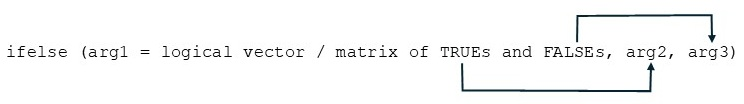
\includegraphics[width=1\linewidth]{pics/ifelse}

\begin{enumerate}
\def\labelenumi{(\roman{enumi})}
\item
  Note the difference between the function \texttt{ifelse()} and the control statement: \texttt{if} - \texttt{else}.
\item
  What arguments are required?
\item
  Study the help file in detail.
\end{enumerate}

\begin{enumerate}
\def\labelenumi{(\alph{enumi})}
\setcounter{enumi}{4}
\item
  The function \texttt{outer()}.

  \begin{enumerate}
  \def\labelenumii{(\roman{enumii})}
  \item
    What arguments are required?
  \item
    Revise our previous example of \texttt{outer()} when constructing a perspective plot with \texttt{persp()}.
  \end{enumerate}
\item
  Work through the following examples and note in particular how the above functions are used together:

  \begin{enumerate}
  \def\labelenumii{(\roman{enumii})}
  \item
    Find the maximum value(s) in each column of the \texttt{LifeCycleSavings} data set.
  \item
    Use \texttt{apply()} together with \texttt{cut()} to divide each column of the LifeCycleSaving data set into low, medium and high.
  \item
    Use \texttt{apply()} to plot each column of the \texttt{LifeCycleSaving} data set against the ratio of \texttt{pop75} to \texttt{pop15} on the x-axis.
  \item
    Use \texttt{apply()} to find the coefficient of variation of each column of the \texttt{LifeCycleSaving} data set.
  \item
    Use \texttt{apply()} together with \texttt{cbind()} and \texttt{rbind()} to obtain a table of the minimum and the maximum values of each column of the LifeCycleSaving data set.
  \item
    Repeat (v) using the airquality data set with and without the elimination of the NAs by using an appropriate function definition in the call to \texttt{apply()}.
  \item
    Use \texttt{sweep()} to convert the \texttt{LifeCycleSaving} data set into standardized scores. Could \texttt{apply()} also be used for this task? Discuss.
  \item
    Use \texttt{ifelse()} to convert negative values in a given vector to zero leaving positive values and missing values unchanged. Illustrate.
  \end{enumerate}
\end{enumerate}

\section{Mapping functions to vectors, dataframes and lists}\label{mapping-functions-to-vectors-dataframes-and-lists}

\begin{enumerate}
\def\labelenumi{(\alph{enumi})}
\item
  Study the functions \texttt{lapply()}, \texttt{sapply()} and \texttt{split()}.
\item
  Carefully study what is produced by the command
\end{enumerate}

\begin{Shaded}
\begin{Highlighting}[]
\FunctionTok{lapply}\NormalTok{ (}\FunctionTok{split}\NormalTok{ (}\FunctionTok{data.frame}\NormalTok{ (state.x77),   }
               \FunctionTok{cut}\NormalTok{ (}\FunctionTok{data.frame}\NormalTok{ (state.x77)}\SpecialCharTok{$}\NormalTok{Illiteracy, }\DecValTok{3}\NormalTok{)), pairs)}
\end{Highlighting}
\end{Shaded}

\pandocbounded{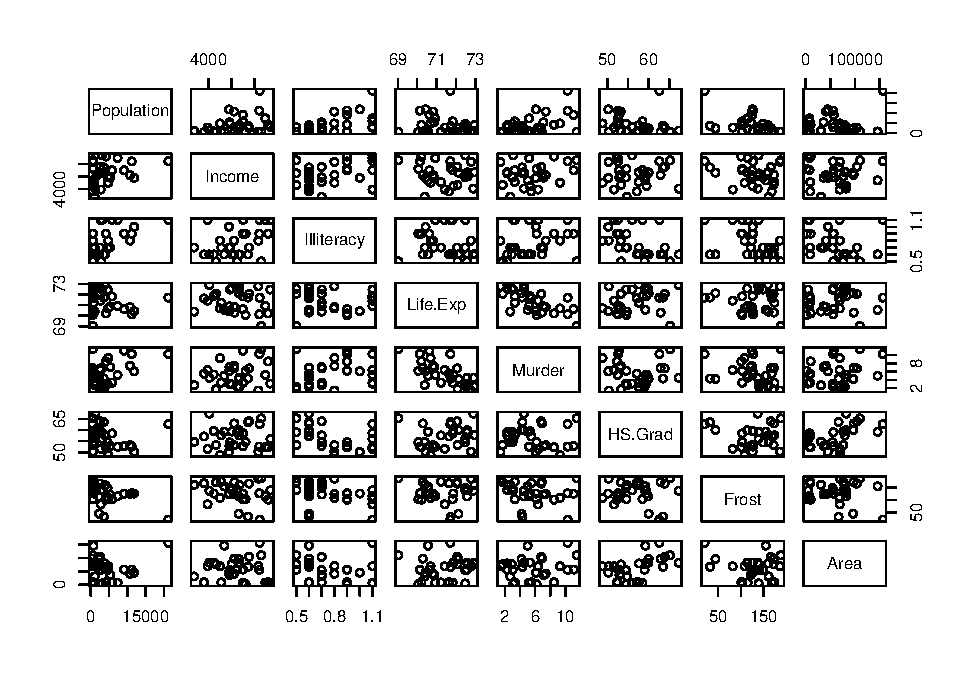
\includegraphics[keepaspectratio]{08-mapping_files/figure-latex/splitExample-1.pdf}} \pandocbounded{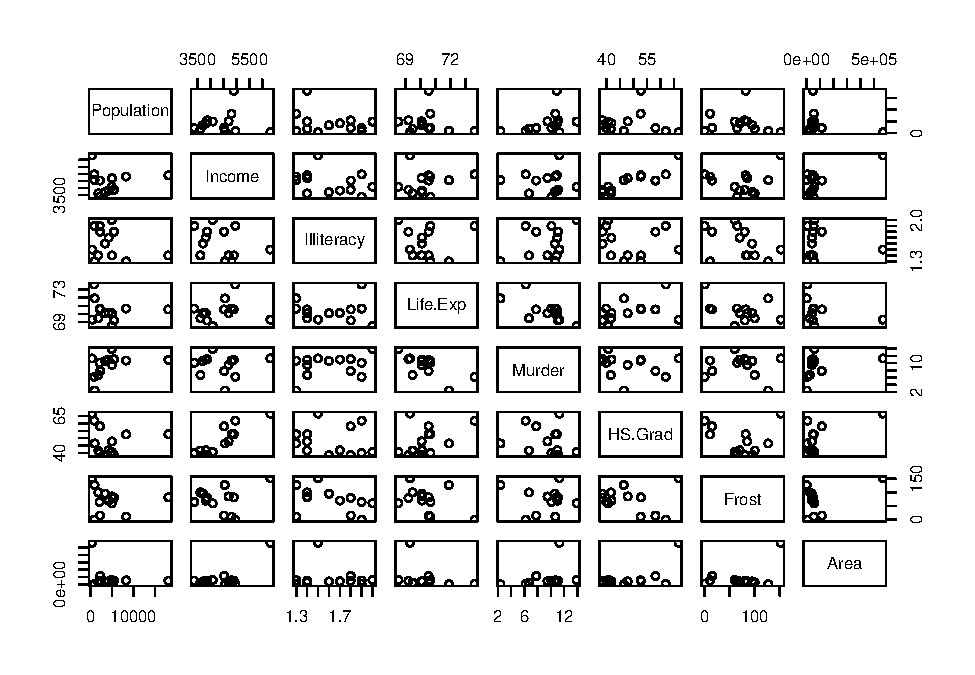
\includegraphics[keepaspectratio]{08-mapping_files/figure-latex/splitExample-2.pdf}} \pandocbounded{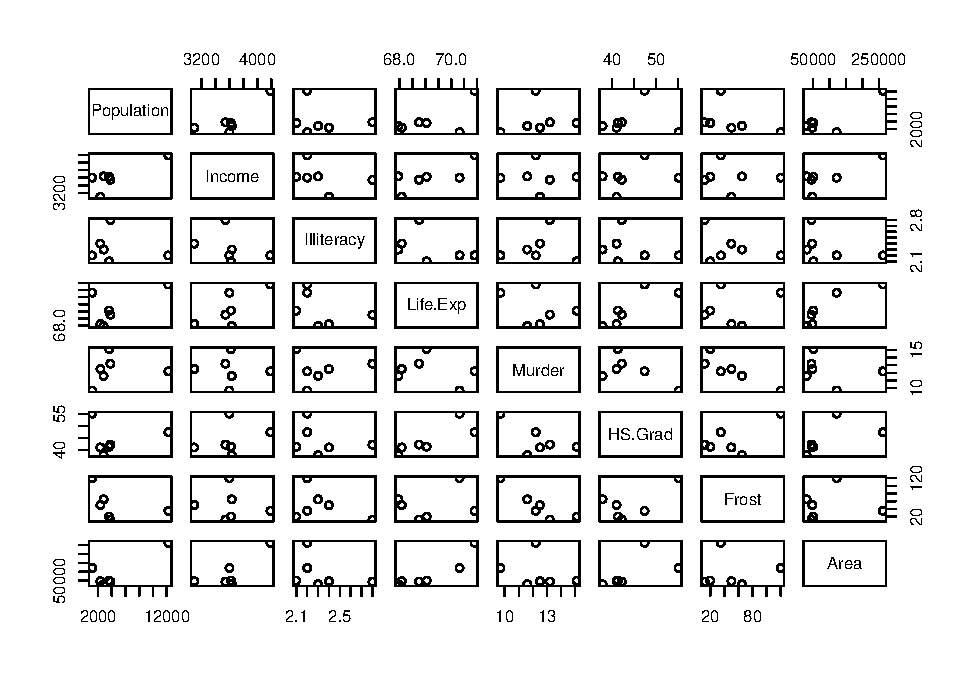
\includegraphics[keepaspectratio]{08-mapping_files/figure-latex/splitExample-3.pdf}}

\begin{verbatim}
#> $`(0.498,1.27]`
#> NULL
#> 
#> $`(1.27,2.03]`
#> NULL
#> 
#> $`(2.03,2.8]`
#> NULL
\end{verbatim}

Note: in order to see all graphs in the R-GUI it is necessary to issue the command

\begin{Shaded}
\begin{Highlighting}[]
\FunctionTok{par}\NormalTok{(}\AttributeTok{ask=}\ConstantTok{TRUE}\NormalTok{) }
\end{Highlighting}
\end{Shaded}

before calling the function \texttt{lapply()}.

\begin{enumerate}
\def\labelenumi{(\alph{enumi})}
\setcounter{enumi}{2}
\tightlist
\item
  Use \texttt{lapply()} to produce histograms of each of the variables in the \texttt{state.x77} data set such that each histogram has as title the correct variable name. The \(x\)- and \(y\)-axis must also be labelled correctly.
\end{enumerate}

\section{\texorpdfstring{The functions: \texttt{mapply()}, \texttt{rapply()} and \texttt{Vectorize()}}{The functions: mapply(), rapply() and Vectorize()}}\label{the-functions-mapply-rapply-and-vectorize}

\begin{enumerate}
\def\labelenumi{(\alph{enumi})}
\tightlist
\item
  To apply a function to more than one list, \texttt{mapply()} is a multivariate version of \texttt{sapply()}. The first argument to \texttt{mapply()} is a function followed by the arguments for that function. The first argument function is applied to each of the elements in the following arguments.
\end{enumerate}

\begin{Shaded}
\begin{Highlighting}[]
\FunctionTok{mapply}\NormalTok{ (}\ControlFlowTok{function}\NormalTok{ (x,y,z) \{x}\SpecialCharTok{+}\NormalTok{y}\SpecialCharTok{+}\NormalTok{z\}, }\AttributeTok{x =} \FunctionTok{c}\NormalTok{(}\DecValTok{2}\NormalTok{, }\DecValTok{3}\NormalTok{), }\AttributeTok{y =} \FunctionTok{c}\NormalTok{(}\DecValTok{4}\NormalTok{,}\DecValTok{5}\NormalTok{), }\AttributeTok{z =} \FunctionTok{c}\NormalTok{(}\DecValTok{1}\NormalTok{,}\DecValTok{8}\NormalTok{))}
\CommentTok{\#\textgreater{} [1]  7 16}
\FunctionTok{mapply}\NormalTok{ (}\ControlFlowTok{function}\NormalTok{(x,y,z) \{ }\FunctionTok{list}\NormalTok{ (}\FunctionTok{min}\NormalTok{ (}\FunctionTok{c}\NormalTok{(x,y,z)), }\FunctionTok{max}\NormalTok{ (}\FunctionTok{c}\NormalTok{(x,y,z))) \}, }
        \AttributeTok{x =} \FunctionTok{c}\NormalTok{(}\DecValTok{2}\NormalTok{, }\DecValTok{3}\NormalTok{), }\AttributeTok{y =} \FunctionTok{c}\NormalTok{(}\DecValTok{4}\NormalTok{, }\DecValTok{5}\NormalTok{), }\AttributeTok{z =} \FunctionTok{c}\NormalTok{(}\DecValTok{1}\NormalTok{, }\DecValTok{8}\NormalTok{))}
\CommentTok{\#\textgreater{}      [,1] [,2]}
\CommentTok{\#\textgreater{} [1,] 1    3   }
\CommentTok{\#\textgreater{} [2,] 4    8}
\end{Highlighting}
\end{Shaded}

\begin{enumerate}
\def\labelenumi{(\alph{enumi})}
\setcounter{enumi}{1}
\tightlist
\item
  Study the help-files of \texttt{rapply()} and \texttt{Vectorize()}.
\end{enumerate}

\section{The mapping function tapply() for grouped data}\label{the-mapping-function-tapply-for-grouped-data}

\begin{enumerate}
\def\labelenumi{(\alph{enumi})}
\tightlist
\item
  Study the arguments of \texttt{tapply()}.
\end{enumerate}

\begin{enumerate}
\def\labelenumi{(\alph{enumi})}
\setcounter{enumi}{1}
\item
  Consider the \texttt{LifeCycleSavings} data set. Create an object \texttt{ddpigrp} that groups the \texttt{LifeCycleSavings} data into four groups G1, G2, G3 and G4 such that G1 members have \texttt{ddpi} within \((0, 2.0]\), G2 members have \texttt{ddpi} within \((2.0, 3.5]\), G3 members have \texttt{ddpi} within \((3.5, 5.0]\), and G4 members have \texttt{ddpi} larger than \(5.0\). Use \texttt{tapply()} to obtain the mean aggregate personal savings of each of the groups defined by \texttt{ddpigrp}.
\item
  If it is needed to break down a vector by more than one categorical variable, a list containing the grouping variables is used as the second argument to \texttt{tapply()}. Illustrate this by finding the mean aggregate personal savings of the groups in \texttt{ddpigrp} broken down by the \texttt{pop15} rating.
\end{enumerate}

\begin{enumerate}
\def\labelenumi{(\alph{enumi})}
\setcounter{enumi}{3}
\tightlist
\item
  In order to use \texttt{tapply()} on more than one variable simultaneously \texttt{apply()} can be used to map \texttt{tapply()} to each of the variables in turn. Study the following command and its output carefully:
\end{enumerate}

\begin{Shaded}
\begin{Highlighting}[]
\NormalTok{ddpigrp }\OtherTok{\textless{}{-}} \FunctionTok{cut}\NormalTok{ (LifeCycleSavings}\SpecialCharTok{$}\NormalTok{ddpi, }
                \AttributeTok{breaks =} \FunctionTok{c}\NormalTok{(}\DecValTok{0}\NormalTok{, }\DecValTok{2}\NormalTok{, }\FloatTok{3.5}\NormalTok{, }\DecValTok{5}\NormalTok{, }\FunctionTok{max}\NormalTok{(LifeCycleSavings}\SpecialCharTok{$}\NormalTok{ddpi)),}
                \AttributeTok{labels =} \FunctionTok{paste0}\NormalTok{ (}\StringTok{"G"}\NormalTok{, }\DecValTok{1}\SpecialCharTok{:}\DecValTok{4}\NormalTok{))}
\FunctionTok{apply}\NormalTok{ (LifeCycleSavings [,}\FunctionTok{c}\NormalTok{ (}\DecValTok{1}\NormalTok{, }\DecValTok{3}\NormalTok{, }\DecValTok{4}\NormalTok{)], }\DecValTok{2}\NormalTok{, }\ControlFlowTok{function}\NormalTok{(x) }
                                           \FunctionTok{tapply}\NormalTok{ (x, ddpigrp, mean)) }
\CommentTok{\#\textgreater{}           sr    pop75       dpi}
\CommentTok{\#\textgreater{} G1  7.855385 1.790769  712.1677}
\CommentTok{\#\textgreater{} G2  8.230625 2.456250 1497.0731}
\CommentTok{\#\textgreater{} G3 11.959000 3.189000 1569.4910}
\CommentTok{\#\textgreater{} G4 11.831818 1.834545  584.6964}
\end{Highlighting}
\end{Shaded}

\begin{enumerate}
\def\labelenumi{(\alph{enumi})}
\setcounter{enumi}{4}
\tightlist
\item
  If \texttt{tapply()} is called without a third argument it returns a vector of the same length than its first argument containing an index into the output that normally would be produced. Illustrate this behaviour and discuss its usage.
\end{enumerate}

\section{\texorpdfstring{The control of execution flow statement if-else and the control functions \texttt{ifelse()} and \texttt{switch()}}{The control of execution flow statement if-else and the control functions ifelse() and switch()}}\label{the-control-of-execution-flow-statement-if-else-and-the-control-functions-ifelse-and-switch}

\begin{enumerate}
\def\labelenumi{(\alph{enumi})}
\tightlist
\item
  The primary tool for conditional computations is the \texttt{if} statement. It takes the form:
\end{enumerate}

\begin{Shaded}
\begin{Highlighting}[]
\NormalTok{if (logical condition evaluating to either TRUE or FALSE)}
\NormalTok{    \{}
\NormalTok{     First set consisting of one or more R expressions}
\NormalTok{    \}}
\NormalTok{else}
\NormalTok{    \{}
\NormalTok{     Second set consisting of one or more R expressions}
\NormalTok{    \} }
\NormalTok{Expression3}
\end{Highlighting}
\end{Shaded}

\begin{enumerate}
\def\labelenumi{(\alph{enumi})}
\setcounter{enumi}{1}
\item
  In the above the \texttt{else} and its accompanying expression(s) are optional.
\item
  If-else statements can be nested.
\item
  Remember that the function \texttt{ifelse()} operates on objects as wholes as illustrated below:
\end{enumerate}

\begin{Shaded}
\begin{Highlighting}[]
\NormalTok{xx }\OtherTok{\textless{}{-}} \FunctionTok{matrix}\NormalTok{(}\DecValTok{1}\SpecialCharTok{:}\DecValTok{25}\NormalTok{, }\AttributeTok{ncol=}\DecValTok{5}\NormalTok{)}
\NormalTok{xx}
\CommentTok{\#\textgreater{}      [,1] [,2] [,3] [,4] [,5]}
\CommentTok{\#\textgreater{} [1,]    1    6   11   16   21}
\CommentTok{\#\textgreater{} [2,]    2    7   12   17   22}
\CommentTok{\#\textgreater{} [3,]    3    8   13   18   23}
\CommentTok{\#\textgreater{} [4,]    4    9   14   19   24}
\CommentTok{\#\textgreater{} [5,]    5   10   15   20   25}
\FunctionTok{ifelse}\NormalTok{(xx }\SpecialCharTok{\textless{}} \DecValTok{10}\NormalTok{, }\DecValTok{0}\NormalTok{, }\DecValTok{1}\NormalTok{)}
\CommentTok{\#\textgreater{}      [,1] [,2] [,3] [,4] [,5]}
\CommentTok{\#\textgreater{} [1,]    0    0    1    1    1}
\CommentTok{\#\textgreater{} [2,]    0    0    1    1    1}
\CommentTok{\#\textgreater{} [3,]    0    0    1    1    1}
\CommentTok{\#\textgreater{} [4,]    0    0    1    1    1}
\CommentTok{\#\textgreater{} [5,]    0    1    1    1    1}
\end{Highlighting}
\end{Shaded}

\begin{enumerate}
\def\labelenumi{(\alph{enumi})}
\setcounter{enumi}{4}
\tightlist
\item
  Note that the function \texttt{match()} can be used as an alternative to multiple if-else statements in certain cases. The function \texttt{match()} takes as first argument a vector, \texttt{x}, of values to be matched and as second argument, \texttt{table}, a vector of possible values to be matched against. A third argument \texttt{nomatch\ =\ NA} specifies the return value if no match occurs. See the example below:
\end{enumerate}

\begin{Shaded}
\begin{Highlighting}[]
\FunctionTok{match}\NormalTok{ (}\FunctionTok{c}\NormalTok{ (}\DecValTok{1}\SpecialCharTok{:}\DecValTok{5}\NormalTok{, }\DecValTok{3}\NormalTok{), }\FunctionTok{c}\NormalTok{ (}\DecValTok{2}\NormalTok{, }\DecValTok{3}\NormalTok{))}
\CommentTok{\#\textgreater{} [1] NA  1  2 NA NA  2}
\FunctionTok{match}\NormalTok{ (}\FunctionTok{c}\NormalTok{ (}\DecValTok{1}\SpecialCharTok{:}\DecValTok{5}\NormalTok{, }\DecValTok{3}\NormalTok{), }\FunctionTok{c}\NormalTok{ (}\DecValTok{2}\NormalTok{, }\DecValTok{3}\NormalTok{), }\AttributeTok{nomatch =} \DecValTok{0}\NormalTok{)}
\CommentTok{\#\textgreater{} [1] 0 1 2 0 0 2}
\FunctionTok{match}\NormalTok{ (}\FunctionTok{c}\NormalTok{ (}\DecValTok{1}\SpecialCharTok{:}\DecValTok{5}\NormalTok{, }\DecValTok{3}\NormalTok{), }\FunctionTok{c}\NormalTok{ (}\DecValTok{3}\NormalTok{, }\DecValTok{2}\NormalTok{), }\AttributeTok{nomatch =} \DecValTok{0}\NormalTok{)}
\CommentTok{\#\textgreater{} [1] 0 2 1 0 0 1}
\end{Highlighting}
\end{Shaded}

\begin{enumerate}
\def\labelenumi{(\alph{enumi})}
\setcounter{enumi}{5}
\tightlist
\item
  The following example provides an illustration of the usage of \texttt{match()}:
\end{enumerate}

\begin{Shaded}
\begin{Highlighting}[]
\NormalTok{month.num }\OtherTok{\textless{}{-}} \DecValTok{5}\SpecialCharTok{:}\DecValTok{9}
\NormalTok{month.name }\OtherTok{\textless{}{-}} \FunctionTok{c}\NormalTok{(}\StringTok{"May"}\NormalTok{, }\StringTok{"June"}\NormalTok{, }\StringTok{"July"}\NormalTok{, }\StringTok{"Aug"}\NormalTok{, }\StringTok{"Sept"}\NormalTok{)}
\NormalTok{new.vec }\OtherTok{\textless{}{-}}\NormalTok{  month.name [}\FunctionTok{match}\NormalTok{ (airquality [, }\StringTok{"Month"}\NormalTok{], month.num)]}
\NormalTok{out }\OtherTok{\textless{}{-}} \FunctionTok{data.frame}\NormalTok{ (airquality [ ,}\DecValTok{1}\SpecialCharTok{:}\DecValTok{5}\NormalTok{], }\AttributeTok{MonthName =}\NormalTok{ new.vec, }
                   \AttributeTok{Day =}\NormalTok{ airquality}\SpecialCharTok{$}\NormalTok{Day)}
\NormalTok{out[}\FunctionTok{c}\NormalTok{(}\DecValTok{1}\SpecialCharTok{:}\DecValTok{5}\NormalTok{,}\DecValTok{148}\SpecialCharTok{:}\DecValTok{153}\NormalTok{), ]}
\CommentTok{\#\textgreater{}     Ozone Solar.R Wind Temp Month MonthName Day}
\CommentTok{\#\textgreater{} 1      41     190  7.4   67     5       May   1}
\CommentTok{\#\textgreater{} 2      36     118  8.0   72     5       May   2}
\CommentTok{\#\textgreater{} 3      12     149 12.6   74     5       May   3}
\CommentTok{\#\textgreater{} 4      18     313 11.5   62     5       May   4}
\CommentTok{\#\textgreater{} 5      NA      NA 14.3   56     5       May   5}
\CommentTok{\#\textgreater{} 148    14      20 16.6   63     9      Sept  25}
\CommentTok{\#\textgreater{} 149    30     193  6.9   70     9      Sept  26}
\CommentTok{\#\textgreater{} 150    NA     145 13.2   77     9      Sept  27}
\CommentTok{\#\textgreater{} 151    14     191 14.3   75     9      Sept  28}
\CommentTok{\#\textgreater{} 152    18     131  8.0   76     9      Sept  29}
\CommentTok{\#\textgreater{} 153    20     223 11.5   68     9      Sept  30}
\end{Highlighting}
\end{Shaded}

\begin{enumerate}
\def\labelenumi{(\alph{enumi})}
\setcounter{enumi}{6}
\tightlist
\item
  The function \texttt{switch()} provides an alternative to a set of nested if-else statements. It takes as first argument, \texttt{EXPR}, an integer value or a character string and as second argument, \texttt{...}, the list of alternatives. As an illustration:
\end{enumerate}

\begin{Shaded}
\begin{Highlighting}[]
\NormalTok{centre }\OtherTok{\textless{}{-}} \ControlFlowTok{function}\NormalTok{(x, type) }
\NormalTok{  \{ }\ControlFlowTok{switch}\NormalTok{(type,}
           \AttributeTok{mean =} \FunctionTok{mean}\NormalTok{(x),}
           \AttributeTok{median =} \FunctionTok{median}\NormalTok{(x),}
           \AttributeTok{trimmed =} \FunctionTok{mean}\NormalTok{(x, }\AttributeTok{trim =} \FloatTok{0.1}\NormalTok{))}
\NormalTok{  \}}

\NormalTok{x }\OtherTok{\textless{}{-}} \FunctionTok{rcauchy}\NormalTok{(}\DecValTok{10}\NormalTok{)}
\NormalTok{x}
\CommentTok{\#\textgreater{}  [1]  {-}3.57418193  {-}4.79099735 {-}79.33502520  {-}0.56487078}
\CommentTok{\#\textgreater{}  [5]  {-}2.26986973   0.10738869   0.39858952   0.04250825}
\CommentTok{\#\textgreater{}  [9]  {-}0.14499379   1.45061262}
\FunctionTok{centre}\NormalTok{(x,}\StringTok{"mean"}\NormalTok{)}
\CommentTok{\#\textgreater{} [1] {-}8.868084}
\FunctionTok{centre}\NormalTok{(x,}\StringTok{"median"}\NormalTok{)}
\CommentTok{\#\textgreater{} [1] {-}0.3549323}
\FunctionTok{centre}\NormalTok{(x,}\StringTok{"trimmed"}\NormalTok{)}
\CommentTok{\#\textgreater{} [1] {-}1.349553}
\end{Highlighting}
\end{Shaded}

\begin{enumerate}
\def\labelenumi{(\alph{enumi})}
\setcounter{enumi}{7}
\tightlist
\item
  The two logical control operators \texttt{\&\&} and \texttt{\textbar{}\textbar{}} are useful when using if-else statements. These two operators operate on logical expressions in contrast to the operators \texttt{\&} and \texttt{\textbar{}} which operate on vectors/matrices.
\end{enumerate}

\section{Loops in R}\label{loops-in-r}

\begin{enumerate}
\def\labelenumi{(\alph{enumi})}
\tightlist
\item
  \texttt{for} loops: The general form is
\end{enumerate}

\begin{Shaded}
\begin{Highlighting}[]
\NormalTok{for (name in values)}
\NormalTok{      \{ expression(s)}
\NormalTok{      \}}
\end{Highlighting}
\end{Shaded}

This type of loop is useful if it is known in advance \emph{{how many times}} the statements in the loop are to be performed. In the above definition values can be either a vector or a list with elements not restricted to be numeric:

\begin{Shaded}
\begin{Highlighting}[]
\ControlFlowTok{for}\NormalTok{ (i }\ControlFlowTok{in} \DecValTok{1}\SpecialCharTok{:}\DecValTok{26}\NormalTok{) }\FunctionTok{cat}\NormalTok{(i, letters[i],}\StringTok{"}\SpecialCharTok{\textbackslash{}n}\StringTok{"}\NormalTok{)}
\CommentTok{\#\textgreater{} 1 a }
\CommentTok{\#\textgreater{} 2 b }
\CommentTok{\#\textgreater{} 3 c }
\CommentTok{\#\textgreater{} 4 d }
\CommentTok{\#\textgreater{} 5 e }
\CommentTok{\#\textgreater{} 6 f }
\CommentTok{\#\textgreater{} 7 g }
\CommentTok{\#\textgreater{} 8 h }
\CommentTok{\#\textgreater{} 9 i }
\CommentTok{\#\textgreater{} 10 j }
\CommentTok{\#\textgreater{} 11 k }
\CommentTok{\#\textgreater{} 12 l }
\CommentTok{\#\textgreater{} 13 m }
\CommentTok{\#\textgreater{} 14 n }
\CommentTok{\#\textgreater{} 15 o }
\CommentTok{\#\textgreater{} 16 p }
\CommentTok{\#\textgreater{} 17 q }
\CommentTok{\#\textgreater{} 18 r }
\CommentTok{\#\textgreater{} 19 s }
\CommentTok{\#\textgreater{} 20 t }
\CommentTok{\#\textgreater{} 21 u }
\CommentTok{\#\textgreater{} 22 v }
\CommentTok{\#\textgreater{} 23 w }
\CommentTok{\#\textgreater{} 24 x }
\CommentTok{\#\textgreater{} 25 y }
\CommentTok{\#\textgreater{} 26 z}
\ControlFlowTok{for}\NormalTok{ (letter }\ControlFlowTok{in}\NormalTok{ letters) }\FunctionTok{cat}\NormalTok{(letter, }\StringTok{"}\SpecialCharTok{\textbackslash{}n}\StringTok{"}\NormalTok{)}
\CommentTok{\#\textgreater{} a }
\CommentTok{\#\textgreater{} b }
\CommentTok{\#\textgreater{} c }
\CommentTok{\#\textgreater{} d }
\CommentTok{\#\textgreater{} e }
\CommentTok{\#\textgreater{} f }
\CommentTok{\#\textgreater{} g }
\CommentTok{\#\textgreater{} h }
\CommentTok{\#\textgreater{} i }
\CommentTok{\#\textgreater{} j }
\CommentTok{\#\textgreater{} k }
\CommentTok{\#\textgreater{} l }
\CommentTok{\#\textgreater{} m }
\CommentTok{\#\textgreater{} n }
\CommentTok{\#\textgreater{} o }
\CommentTok{\#\textgreater{} p }
\CommentTok{\#\textgreater{} q }
\CommentTok{\#\textgreater{} r }
\CommentTok{\#\textgreater{} s }
\CommentTok{\#\textgreater{} t }
\CommentTok{\#\textgreater{} u }
\CommentTok{\#\textgreater{} v }
\CommentTok{\#\textgreater{} w }
\CommentTok{\#\textgreater{} x }
\CommentTok{\#\textgreater{} y }
\CommentTok{\#\textgreater{} z}
\end{Highlighting}
\end{Shaded}

Consider a list consisting of several matrices, each with different numbers of rows but the same number of columns. Write an R function that will create a single matrix consisting of all the elements of the given list concatenated by rows.

\begin{enumerate}
\def\labelenumi{(\alph{enumi})}
\setcounter{enumi}{1}
\tightlist
\item
  \texttt{while} loops: The general form is
\end{enumerate}

\begin{Shaded}
\begin{Highlighting}[]
\NormalTok{while (condition)}
\NormalTok{        \{ expression(s)}
\NormalTok{        \}}
\end{Highlighting}
\end{Shaded}

This type of loop continues while condition evaluates to TRUE.

\begin{enumerate}
\def\labelenumi{(\alph{enumi})}
\setcounter{enumi}{2}
\tightlist
\item
  Control inside loops: \texttt{next} and \texttt{break}
\end{enumerate}

The command \texttt{next} is used to skip over any remaining statements in the loop and continue executing. The command \texttt{break} causes the immediate exit from the loop. In nested loops these commands apply to the most recently opened loop.

\begin{enumerate}
\def\labelenumi{(\alph{enumi})}
\setcounter{enumi}{3}
\tightlist
\item
  \texttt{repeat} loops: The general form is
\end{enumerate}

\begin{Shaded}
\begin{Highlighting}[]
\NormalTok{repeat \{ expression(s)}
\NormalTok{       \}}
\end{Highlighting}
\end{Shaded}

This type of loop continues until a break command is encountered.

\begin{enumerate}
\def\labelenumi{(\alph{enumi})}
\setcounter{enumi}{4}
\item
  Remember that many operations that might be handled by loops can be more efficiently performed in R by using the subscripting tools discussed earlier.
\item
  As a further example we will consider the calculation of the Pearson chi-squared statistic for the test of independence in a two-way classification table:
\end{enumerate}

\[
\chi^2_p = \sum_{i=1}^r \sum_{j=1}^c \frac{(f_{ij}-e_{ij})^2}{e_{ij}}
\]

with \(e_{ij} = \frac{f_{i.}f_{.j}}{f_{..}}\) the expected frequencies. This statistic can be calculated in R without using loops as follows:

\begin{Shaded}
\begin{Highlighting}[]
\NormalTok{fi. }\OtherTok{\textless{}{-}}\NormalTok{ ftable }\SpecialCharTok{\%*\%} \FunctionTok{rep}\NormalTok{ (}\DecValTok{1}\NormalTok{, }\FunctionTok{ncol}\NormalTok{ (ftable))}
\NormalTok{f.j }\OtherTok{\textless{}{-}} \FunctionTok{rep}\NormalTok{ (}\DecValTok{1}\NormalTok{, }\FunctionTok{nrow}\NormalTok{ (ftable)) }\SpecialCharTok{\%*\%}\NormalTok{ ftable}
\NormalTok{e }\OtherTok{\textless{}{-}}\NormalTok{ (fi. }\SpecialCharTok{\%*\%}\NormalTok{ f.j)}\SpecialCharTok{/}\FunctionTok{sum}\NormalTok{(fi.)}
\NormalTok{X2p }\OtherTok{\textless{}{-}} \FunctionTok{sum}\NormalTok{ ( (ftable}\SpecialCharTok{{-}}\NormalTok{e)}\SpecialCharTok{\^{}}\DecValTok{2} \SpecialCharTok{/}\NormalTok{e)}
\end{Highlighting}
\end{Shaded}

Explicit loops in R can potentially be expensive in terms of time and memory. The functions \texttt{apply()}, \texttt{tapply()}, \texttt{sapply()} and \texttt{lapply()} should be used instead if possible. The expected frequencies in the previous example can, for example, be obtained as follows:

\begin{Shaded}
\begin{Highlighting}[]
\NormalTok{e.freq }\OtherTok{\textless{}{-}} \FunctionTok{outer}\NormalTok{ (}\FunctionTok{apply}\NormalTok{ (ftable, }\DecValTok{1}\NormalTok{, sum),  }\FunctionTok{apply}\NormalTok{ (ftable, }\DecValTok{2}\NormalTok{, sum)) }\SpecialCharTok{/} \FunctionTok{sum}\NormalTok{(ftable)}
\end{Highlighting}
\end{Shaded}

\section{The execution time of R tasks}\label{the-execution-time-of-r-tasks}

The functions \texttt{system.time()} and \texttt{proc.time()} provide information regarding the execution of R tasks.

\begin{enumerate}
\def\labelenumi{(\alph{enumi})}
\tightlist
\item
  \texttt{proc.time} determines how much real and CPU time (in seconds) the currently running R process has already take:
\end{enumerate}

\begin{Shaded}
\begin{Highlighting}[]
\FunctionTok{proc.time}\NormalTok{()   }\CommentTok{\# called with no arguments}
\CommentTok{\#\textgreater{}    user  system elapsed }
\CommentTok{\#\textgreater{}    0.57    0.04    3.01}
\end{Highlighting}
\end{Shaded}

\begin{enumerate}
\def\labelenumi{(\alph{enumi})}
\setcounter{enumi}{1}
\tightlist
\item
  \texttt{system.time(expr)} calls the function \texttt{proc.time()}, evaluates \texttt{expr}, and then calls \texttt{proc.time()} once more, returning the difference between the two \texttt{proc.time()} calls:
\end{enumerate}

\begin{Shaded}
\begin{Highlighting}[]
\FunctionTok{system.time}\NormalTok{ (}\FunctionTok{hist}\NormalTok{ (}\FunctionTok{rev}\NormalTok{ (}\FunctionTok{sort}\NormalTok{ (}\FunctionTok{rnorm}\NormalTok{ (}\DecValTok{1000000}\NormalTok{)))))}
\end{Highlighting}
\end{Shaded}

\pandocbounded{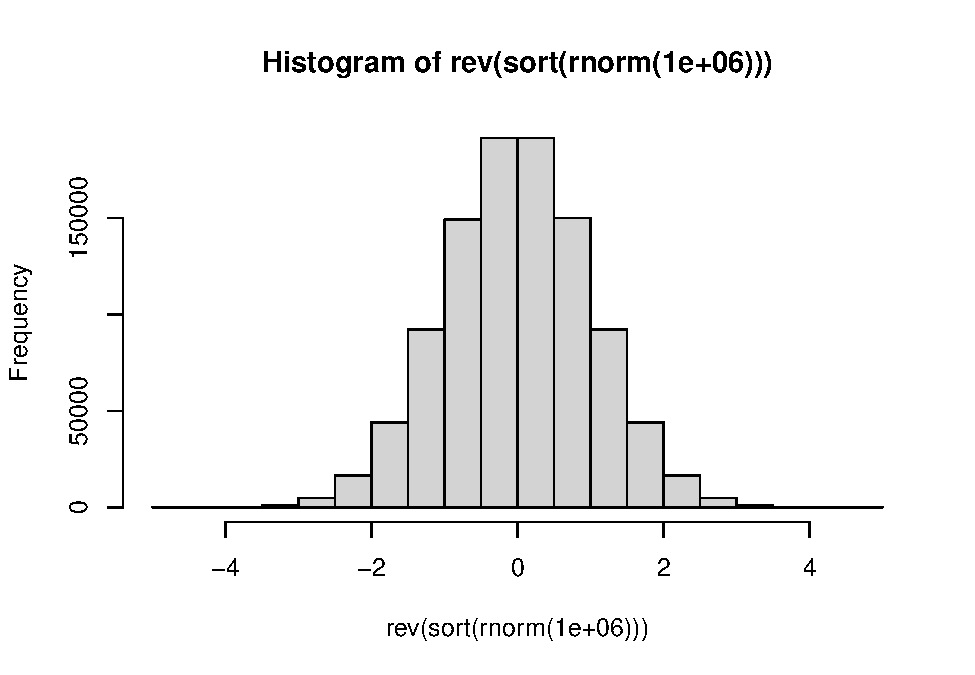
\includegraphics[keepaspectratio]{08-mapping_files/figure-latex/systemtimeExample-1.pdf}}

\begin{verbatim}
#>    user  system elapsed 
#>    0.18    0.00    0.20
\end{verbatim}

Note that user and system times do not necessarily add up to elapsed time exactly.

\begin{enumerate}
\def\labelenumi{(\alph{enumi})}
\setcounter{enumi}{2}
\item
  Write the necessary code using \texttt{proc.time()} directly to obtain the execution time of \texttt{hist\ (rev\ (sort\ (rnorm\ (1000000))))}.
\item
  As an application of \texttt{system.time()} and \texttt{proc.time()} perform the following simulation study: Given a covariance matrix \(\mathbf{S}:p \times p\) the task is to compute the corresponding correlation matrix. The execution times of the following three methods are to be compared:

  \begin{enumerate}
  \def\labelenumii{(\roman{enumii})}
  \item
    Direct elementwise calculation of \(r_{ij} = \frac{s_{ij}}{\sqrt{s_{ii}s_{jj}}}\) using two nested for loops;
  \item
    Two applications of \texttt{sweep()};
  \item
    Matrix multiplication where \(\mathbf{R}:p \times p = [diag(\mathbf{S})]^{-\frac{1}{2}} \mathbf{S} [diag(\mathbf{S})]^{-\frac{1}{2}}\) where \(diag(\mathbf{A})\) denotes the diagonal matrix formed from \(\mathbf{A}:p \times p\) by setting all its off-diagonal elements equal to zero.
  \end{enumerate}
\end{enumerate}

Use \texttt{var()} and \texttt{rnorm()} to compute covariance matrices of different sizes \(p\) from samples varying in size \(n\). Study the role of \(n\) and \(p\) in the effectiveness (economy in execution time) of the above three methods. Display the results graphically. Remember that for valid comparisons the three methods must be executed with identical samples.

\section{The calling of functions with argument lists}\label{the-calling-of-functions-with-argument-lists}

\begin{enumerate}
\def\labelenumi{(\alph{enumi})}
\tightlist
\item
  The function \texttt{do.call()} provides an alternative to the usual method of calling functions by name. It allows specifying the name of the function with its arguments in the form of a list:
\end{enumerate}

\begin{Shaded}
\begin{Highlighting}[]
\FunctionTok{mean}\NormalTok{ ( }\FunctionTok{c}\NormalTok{ (}\DecValTok{1}\SpecialCharTok{:}\DecValTok{100}\NormalTok{, }\DecValTok{500}\NormalTok{), }\AttributeTok{trim=}\FloatTok{0.1}\NormalTok{)}
\CommentTok{\#\textgreater{} [1] 51}
\FunctionTok{do.call}\NormalTok{ (}\StringTok{"mean"}\NormalTok{, }\FunctionTok{list}\NormalTok{( }\FunctionTok{c}\NormalTok{ (}\DecValTok{1}\SpecialCharTok{:}\DecValTok{100}\NormalTok{, }\DecValTok{500}\NormalTok{), }\AttributeTok{trim=}\FloatTok{0.1}\NormalTok{))}
\CommentTok{\#\textgreater{} [1] 51}
\end{Highlighting}
\end{Shaded}

\begin{enumerate}
\def\labelenumi{(\alph{enumi})}
\setcounter{enumi}{1}
\item
  How does \texttt{do.call()} differ from the function \texttt{call()}?
\item
  As an illustration of the usage of \texttt{do.call()} study the following example:
\end{enumerate}

\begin{Shaded}
\begin{Highlighting}[]
\NormalTok{na.pattern }\OtherTok{\textless{}{-}} \ControlFlowTok{function}\NormalTok{(frame)}
\NormalTok{\{ nas }\OtherTok{\textless{}{-}} \FunctionTok{is.na}\NormalTok{ (frame)}
  \FunctionTok{storage.mode}\NormalTok{ (nas) }\OtherTok{\textless{}{-}} \StringTok{"integer"}
  \FunctionTok{table}\NormalTok{ (}\FunctionTok{do.call}\NormalTok{ (}\StringTok{"paste"}\NormalTok{, }\FunctionTok{c}\NormalTok{(}\FunctionTok{as.data.frame}\NormalTok{(nas), }\AttributeTok{sep =} \StringTok{""}\NormalTok{)))}
\NormalTok{\}}
\FunctionTok{na.pattern}\NormalTok{(}\FunctionTok{as.data.frame}\NormalTok{(airquality))}
\CommentTok{\#\textgreater{} }
\CommentTok{\#\textgreater{} 000000 010000 100000 110000 }
\CommentTok{\#\textgreater{}    111      5     35      2}
\end{Highlighting}
\end{Shaded}

What can be learned from the above output?

\begin{enumerate}
\def\labelenumi{(\alph{enumi})}
\setcounter{enumi}{3}
\tightlist
\item
  What is the difference between \texttt{as.integer()}, \texttt{storage.mode()\ \textless{}–\ "integer"}, \texttt{storage.mode()} and \texttt{mode()}?
\end{enumerate}

\section{Evaluating R strings a commands}\label{evaluating-r-strings-a-commands}

Recall from Figure \ref{fig:expression} that the function \texttt{parse(text\ =\ "3\ +\ 4")} returns the unevaluated expression \texttt{3\ +\ 4}. In order to evaluate the expression use function \texttt{eval()}: \texttt{eval\ (parse\ (text\ =\ "3\ +\ 4"))} returns \texttt{7}.

\section{Object oriented programming in R}\label{object-oriented-programming-in-r}

Suppose we would like to investigate the body of function \texttt{plot()}. We know that this can be done by entering the function's name at the R prompt:

\begin{Shaded}
\begin{Highlighting}[]
\NormalTok{plot}
\CommentTok{\#\textgreater{} function (x, y, ...) }
\CommentTok{\#\textgreater{} UseMethod("plot")}
\CommentTok{\#\textgreater{} \textless{}bytecode: 0x000001ecea12a8f0\textgreater{}}
\CommentTok{\#\textgreater{} \textless{}environment: namespace:base\textgreater{}}
\end{Highlighting}
\end{Shaded}

The presence of \texttt{UseMethod("plot")} shows that \texttt{plot()} is a \emph{{generic}} function. The \emph{{class}} of an object determines how it will be treated by a generic function i.e.~what \emph{{method}} will be applied to it. Function \texttt{setClass()} is used for setting the class attribute of an object. Function \texttt{methods()} is used to find out (a) what is the repertoire of methods of a generic function and (b) what methods are available for a certain class:

\begin{Shaded}
\begin{Highlighting}[]
\FunctionTok{methods}\NormalTok{(plot) }\CommentTok{\# repertoire of methods for FUNCTION plot()}
\CommentTok{\#\textgreater{}  [1] plot.acf*           plot.data.frame*   }
\CommentTok{\#\textgreater{}  [3] plot.decomposed.ts* plot.default       }
\CommentTok{\#\textgreater{}  [5] plot.dendrogram*    plot.density*      }
\CommentTok{\#\textgreater{}  [7] plot.ecdf           plot.factor*       }
\CommentTok{\#\textgreater{}  [9] plot.formula*       plot.function      }
\CommentTok{\#\textgreater{} [11] plot.hclust*        plot.histogram*    }
\CommentTok{\#\textgreater{} [13] plot.HoltWinters*   plot.isoreg*       }
\CommentTok{\#\textgreater{} [15] plot.lm*            plot.medpolish*    }
\CommentTok{\#\textgreater{} [17] plot.mlm*           plot.ppr*          }
\CommentTok{\#\textgreater{} [19] plot.prcomp*        plot.princomp*     }
\CommentTok{\#\textgreater{} [21] plot.profile*       plot.profile.nls*  }
\CommentTok{\#\textgreater{} [23] plot.raster*        plot.spec*         }
\CommentTok{\#\textgreater{} [25] plot.stepfun        plot.stl*          }
\CommentTok{\#\textgreater{} [27] plot.table*         plot.ts            }
\CommentTok{\#\textgreater{} [29] plot.tskernel*      plot.TukeyHSD*     }
\CommentTok{\#\textgreater{} see \textquotesingle{}?methods\textquotesingle{} for accessing help and source code}
\FunctionTok{methods}\NormalTok{(}\AttributeTok{class=}\StringTok{"lm"}\NormalTok{)  }\CommentTok{\# what methods are available for CLASS lm}
\CommentTok{\#\textgreater{}  [1] add1           alias          anova         }
\CommentTok{\#\textgreater{}  [4] case.names     coerce         confint       }
\CommentTok{\#\textgreater{}  [7] cooks.distance deviance       dfbeta        }
\CommentTok{\#\textgreater{} [10] dfbetas        drop1          dummy.coef    }
\CommentTok{\#\textgreater{} [13] effects        extractAIC     family        }
\CommentTok{\#\textgreater{} [16] formula        hatvalues      influence     }
\CommentTok{\#\textgreater{} [19] initialize     kappa          labels        }
\CommentTok{\#\textgreater{} [22] logLik         model.frame    model.matrix  }
\CommentTok{\#\textgreater{} [25] nobs           plot           predict       }
\CommentTok{\#\textgreater{} [28] print          proj           qr            }
\CommentTok{\#\textgreater{} [31] residuals      rstandard      rstudent      }
\CommentTok{\#\textgreater{} [34] show           simulate       slotsFromS3   }
\CommentTok{\#\textgreater{} [37] summary        variable.names vcov          }
\CommentTok{\#\textgreater{} see \textquotesingle{}?methods\textquotesingle{} for accessing help and source code}
\end{Highlighting}
\end{Shaded}

In broad terms there are currently three types of classes in use in R: The old classes or S3 classes and the newer S4 and S5 (also called \emph{{reference classes}}) classes. The newer classes can contain one or more \emph{{slots}} which can be accessed using the operator \texttt{@}. Central to the concept of object oriented programming is that a method can inherit from another method. The function \texttt{NextMethod()} provides a mechanism for \emph{{inheritance}}.

\begin{enumerate}
\def\labelenumi{(\alph{enumi})}
\item
  As an example of a generic function study the example in the help file of the function \texttt{all.equal()}.
\item
  R provides many more facilities for writing object oriented functions. Consult the \href{https://cran.r-project.org/doc/manuals/r-release/R-lang.pdf}{R Language Definition Manual} Chapter 5: Object-Oriented Programming for further details.
\item
  A statistical investigation is often concerned with survey or questionnaire data where respondents must select one of several categorical alternatives. The \texttt{questdata} below shows the responses made by 10 respondents on four questions. The alternatives for each question were measured on a five point categorical scale. We can refer to the \texttt{questdata\ dataframe} as the full data. This form of representing the data is not an effective way of storing the data when the number of respondents is large. A more compact way of saving the data without any loss in information is to store the data in the form of a \emph{{response pattern}} matrix or dataframe. The first row of \texttt{questdata} constitutes one particular response pattern namely \texttt{("b"\ "c"\ "a"\ "d")}. A response pattern matrix (dataframe) shows all the unique response patterns together with the frequency with which each of the different response patterns has occurred. Your challenge is to provide the necessary R functions to convert the full data into a response pattern representation, and conversely to recover the full data from its response pattern representation.
\end{enumerate}

\begin{Shaded}
\begin{Highlighting}[]
\NormalTok{questdata }\OtherTok{\textless{}{-}} \FunctionTok{rbind}\NormalTok{ (}\FunctionTok{c}\NormalTok{(}\StringTok{"b"}\NormalTok{, }\StringTok{"c"}\NormalTok{, }\StringTok{"a"}\NormalTok{, }\StringTok{"d"}\NormalTok{),}
                    \FunctionTok{c}\NormalTok{(}\StringTok{"d"}\NormalTok{, }\StringTok{"d"}\NormalTok{, }\StringTok{"c"}\NormalTok{, }\StringTok{"a"}\NormalTok{),}
                    \FunctionTok{c}\NormalTok{(}\StringTok{"a"}\NormalTok{, }\StringTok{"d"}\NormalTok{, }\StringTok{"c"}\NormalTok{, }\StringTok{"e"}\NormalTok{),}
                    \FunctionTok{c}\NormalTok{(}\StringTok{"a"}\NormalTok{, }\StringTok{"d"}\NormalTok{, }\StringTok{"c"}\NormalTok{, }\StringTok{"e"}\NormalTok{),}
                    \FunctionTok{c}\NormalTok{(}\StringTok{"b"}\NormalTok{, }\StringTok{"c"}\NormalTok{, }\StringTok{"a"}\NormalTok{, }\StringTok{"d"}\NormalTok{),}
                    \FunctionTok{c}\NormalTok{(}\StringTok{"a"}\NormalTok{, }\StringTok{"d"}\NormalTok{, }\StringTok{"c"}\NormalTok{, }\StringTok{"e"}\NormalTok{),}
                    \FunctionTok{c}\NormalTok{(}\StringTok{"b"}\NormalTok{, }\StringTok{"c"}\NormalTok{, }\StringTok{"a"}\NormalTok{, }\StringTok{"d"}\NormalTok{),}
                    \FunctionTok{c}\NormalTok{(}\StringTok{"d"}\NormalTok{, }\StringTok{"d"}\NormalTok{, }\StringTok{"c"}\NormalTok{, }\StringTok{"a"}\NormalTok{),}
                    \FunctionTok{c}\NormalTok{(}\StringTok{"c"}\NormalTok{, }\StringTok{"b"}\NormalTok{, }\StringTok{"a"}\NormalTok{, }\StringTok{"e"}\NormalTok{),}
                    \FunctionTok{c}\NormalTok{(}\StringTok{"b"}\NormalTok{, }\StringTok{"c"}\NormalTok{, }\StringTok{"a"}\NormalTok{, }\StringTok{"d"}\NormalTok{))}
\FunctionTok{colnames}\NormalTok{(questdata) }\OtherTok{\textless{}{-}} \FunctionTok{c}\NormalTok{(}\StringTok{"Q1"}\NormalTok{, }\StringTok{"Q2"}\NormalTok{, }\StringTok{"Q3"}\NormalTok{, }\StringTok{"Q4"}\NormalTok{)}
\end{Highlighting}
\end{Shaded}

\begin{enumerate}
\def\labelenumi{(\roman{enumi})}
\tightlist
\item
  Create the R object \texttt{questdata} and then give the following instructions:
\end{enumerate}

\begin{Shaded}
\begin{Highlighting}[]
\FunctionTok{unique}\NormalTok{ (questdata [,}\DecValTok{1}\NormalTok{])}
\CommentTok{\#\textgreater{} [1] "b" "d" "a" "c"}
\FunctionTok{duplicated}\NormalTok{ (questdata)}
\CommentTok{\#\textgreater{}  [1] FALSE FALSE FALSE  TRUE  TRUE  TRUE  TRUE  TRUE FALSE}
\CommentTok{\#\textgreater{} [10]  TRUE}
\FunctionTok{duplicated}\NormalTok{ (questdata, }\AttributeTok{MARGIN =} \DecValTok{1}\NormalTok{)}
\CommentTok{\#\textgreater{}  [1] FALSE FALSE FALSE  TRUE  TRUE  TRUE  TRUE  TRUE FALSE}
\CommentTok{\#\textgreater{} [10]  TRUE}
\FunctionTok{duplicated}\NormalTok{ (questdata, }\AttributeTok{MARGIN =} \DecValTok{2}\NormalTok{)}
\CommentTok{\#\textgreater{}    Q1    Q2    Q3    Q4 }
\CommentTok{\#\textgreater{} FALSE FALSE FALSE FALSE}
\FunctionTok{unique}\NormalTok{ (questdata)}
\CommentTok{\#\textgreater{}      Q1  Q2  Q3  Q4 }
\CommentTok{\#\textgreater{} [1,] "b" "c" "a" "d"}
\CommentTok{\#\textgreater{} [2,] "d" "d" "c" "a"}
\CommentTok{\#\textgreater{} [3,] "a" "d" "c" "e"}
\CommentTok{\#\textgreater{} [4,] "c" "b" "a" "e"}
\FunctionTok{unique}\NormalTok{ (questdata, }\AttributeTok{MARGIN =} \DecValTok{1}\NormalTok{)}
\CommentTok{\#\textgreater{}      Q1  Q2  Q3  Q4 }
\CommentTok{\#\textgreater{} [1,] "b" "c" "a" "d"}
\CommentTok{\#\textgreater{} [2,] "d" "d" "c" "a"}
\CommentTok{\#\textgreater{} [3,] "a" "d" "c" "e"}
\CommentTok{\#\textgreater{} [4,] "c" "b" "a" "e"}
\FunctionTok{unique}\NormalTok{ (questdata, }\AttributeTok{MARGIN =} \DecValTok{2}\NormalTok{)}
\CommentTok{\#\textgreater{}       Q1  Q2  Q3  Q4 }
\CommentTok{\#\textgreater{}  [1,] "b" "c" "a" "d"}
\CommentTok{\#\textgreater{}  [2,] "d" "d" "c" "a"}
\CommentTok{\#\textgreater{}  [3,] "a" "d" "c" "e"}
\CommentTok{\#\textgreater{}  [4,] "a" "d" "c" "e"}
\CommentTok{\#\textgreater{}  [5,] "b" "c" "a" "d"}
\CommentTok{\#\textgreater{}  [6,] "a" "d" "c" "e"}
\CommentTok{\#\textgreater{}  [7,] "b" "c" "a" "d"}
\CommentTok{\#\textgreater{}  [8,] "d" "d" "c" "a"}
\CommentTok{\#\textgreater{}  [9,] "c" "b" "a" "e"}
\CommentTok{\#\textgreater{} [10,] "b" "c" "a" "d"}
\end{Highlighting}
\end{Shaded}

\begin{enumerate}
\def\labelenumi{(\roman{enumi})}
\setcounter{enumi}{1}
\tightlist
\item
  Examine Table \ref{tab:MatrixFunc} and carefully describe the behaviour of the functions \texttt{duplicated()} and \texttt{unique()}.
\end{enumerate}

\begin{enumerate}
\def\labelenumi{(\roman{enumi})}
\setcounter{enumi}{2}
\item
  Write an R function, say \texttt{full2resp} to obtain the response pattern representation of questionnaire data like those given above. Test your function on \texttt{questdata}.
\item
  Write an R function, say \texttt{resp2full} to obtain the full data set given its response pattern representation. Test your function on the response pattern representation of the \texttt{questdata}.
\end{enumerate}

\section{Recursion}\label{recursion}

Functions in R can call themselves. This process is called \emph{{recursion}} and it is implemented in R programming by the function \texttt{Recall()}.

\begin{enumerate}
\def\labelenumi{(\alph{enumi})}
\tightlist
\item
  As an example we will use recursion to calculate \(x(x+1)(x+2)\dots(x+k)\) with \(k\) a positive integer:
\end{enumerate}

\begin{Shaded}
\begin{Highlighting}[]
\NormalTok{recurs.example }\OtherTok{\textless{}{-}} \ControlFlowTok{function}\NormalTok{ (x, k) }
\NormalTok{\{ }\CommentTok{\# Function to calculate x(x+1)(x+2).....(x+k)}
  \CommentTok{\# where k is a positive integer.}
     \ControlFlowTok{if}\NormalTok{ (k }\SpecialCharTok{\textless{}} \DecValTok{0}\NormalTok{ ) }
      \FunctionTok{stop}\NormalTok{(}\StringTok{"k not allowed to be negative or non{-}integer"}\NormalTok{)}
    \ControlFlowTok{else} \ControlFlowTok{if}\NormalTok{( k }\SpecialCharTok{==} \DecValTok{0}\NormalTok{) x}
       \ControlFlowTok{else}\NormalTok{(x}\SpecialCharTok{+}\NormalTok{k) }\SpecialCharTok{*} \FunctionTok{Recall}\NormalTok{(x,k}\DecValTok{{-}1}\NormalTok{)}
\NormalTok{   \}}
\end{Highlighting}
\end{Shaded}

Investigate if \texttt{recurs.example()} works correctly.

\begin{enumerate}
\def\labelenumi{(\alph{enumi})}
\setcounter{enumi}{1}
\tightlist
\item
  Explain how recursion works by studying the output of the following function for values of \(r = 1, 2, 3, 4, 5, 6\):
\end{enumerate}

\begin{Shaded}
\begin{Highlighting}[]
\NormalTok{Recursiontest }\OtherTok{\textless{}{-}} \ControlFlowTok{function}\NormalTok{ (r)}
\NormalTok{\{ }\ControlFlowTok{if}\NormalTok{ (r }\SpecialCharTok{\textless{}=} \DecValTok{0}\NormalTok{) }\ConstantTok{NULL}
  \ControlFlowTok{else}\NormalTok{ \{ }\FunctionTok{cat}\NormalTok{(}\StringTok{"Write = "}\NormalTok{, r, }\StringTok{"}\SpecialCharTok{\textbackslash{}n}\StringTok{"}\NormalTok{)}
         \FunctionTok{Recall}\NormalTok{ (r }\SpecialCharTok{{-}} \DecValTok{1}\NormalTok{)}
         \FunctionTok{Recall}\NormalTok{ (r }\SpecialCharTok{{-}} \DecValTok{2}\NormalTok{)}
\NormalTok{       \}}
\NormalTok{\}}
\FunctionTok{Recursiontest}\NormalTok{(}\DecValTok{1}\NormalTok{)}
\CommentTok{\#\textgreater{} Write =  1}
\CommentTok{\#\textgreater{} NULL}
\FunctionTok{Recursiontest}\NormalTok{(}\DecValTok{2}\NormalTok{)}
\CommentTok{\#\textgreater{} Write =  2 }
\CommentTok{\#\textgreater{} Write =  1}
\CommentTok{\#\textgreater{} NULL}
\FunctionTok{Recursiontest}\NormalTok{(}\DecValTok{3}\NormalTok{)}
\CommentTok{\#\textgreater{} Write =  3 }
\CommentTok{\#\textgreater{} Write =  2 }
\CommentTok{\#\textgreater{} Write =  1 }
\CommentTok{\#\textgreater{} Write =  1}
\CommentTok{\#\textgreater{} NULL}
\FunctionTok{Recursiontest}\NormalTok{(}\DecValTok{4}\NormalTok{)}
\CommentTok{\#\textgreater{} Write =  4 }
\CommentTok{\#\textgreater{} Write =  3 }
\CommentTok{\#\textgreater{} Write =  2 }
\CommentTok{\#\textgreater{} Write =  1 }
\CommentTok{\#\textgreater{} Write =  1 }
\CommentTok{\#\textgreater{} Write =  2 }
\CommentTok{\#\textgreater{} Write =  1}
\CommentTok{\#\textgreater{} NULL}
\FunctionTok{Recursiontest}\NormalTok{(}\DecValTok{5}\NormalTok{)}
\CommentTok{\#\textgreater{} Write =  5 }
\CommentTok{\#\textgreater{} Write =  4 }
\CommentTok{\#\textgreater{} Write =  3 }
\CommentTok{\#\textgreater{} Write =  2 }
\CommentTok{\#\textgreater{} Write =  1 }
\CommentTok{\#\textgreater{} Write =  1 }
\CommentTok{\#\textgreater{} Write =  2 }
\CommentTok{\#\textgreater{} Write =  1 }
\CommentTok{\#\textgreater{} Write =  3 }
\CommentTok{\#\textgreater{} Write =  2 }
\CommentTok{\#\textgreater{} Write =  1 }
\CommentTok{\#\textgreater{} Write =  1}
\CommentTok{\#\textgreater{} NULL}
\FunctionTok{Recursiontest}\NormalTok{(}\DecValTok{6}\NormalTok{)}
\CommentTok{\#\textgreater{} Write =  6 }
\CommentTok{\#\textgreater{} Write =  5 }
\CommentTok{\#\textgreater{} Write =  4 }
\CommentTok{\#\textgreater{} Write =  3 }
\CommentTok{\#\textgreater{} Write =  2 }
\CommentTok{\#\textgreater{} Write =  1 }
\CommentTok{\#\textgreater{} Write =  1 }
\CommentTok{\#\textgreater{} Write =  2 }
\CommentTok{\#\textgreater{} Write =  1 }
\CommentTok{\#\textgreater{} Write =  3 }
\CommentTok{\#\textgreater{} Write =  2 }
\CommentTok{\#\textgreater{} Write =  1 }
\CommentTok{\#\textgreater{} Write =  1 }
\CommentTok{\#\textgreater{} Write =  4 }
\CommentTok{\#\textgreater{} Write =  3 }
\CommentTok{\#\textgreater{} Write =  2 }
\CommentTok{\#\textgreater{} Write =  1 }
\CommentTok{\#\textgreater{} Write =  1 }
\CommentTok{\#\textgreater{} Write =  2 }
\CommentTok{\#\textgreater{} Write =  1}
\CommentTok{\#\textgreater{} NULL}
\end{Highlighting}
\end{Shaded}

\begin{enumerate}
\def\labelenumi{(\alph{enumi})}
\setcounter{enumi}{2}
\item
  Use recursion and the function \texttt{Recall()} to write an R function to calculate \(x!\).
\item
  Use recursion to write an R function that generates a matrix whose rows contain subsets of size \(r\) of the first \(n\) elements of the vector \texttt{v}. Ignore the possibility of repeated values in \texttt{v} and give this vector the default value of \texttt{1:n}.
\end{enumerate}

\section{Environments in R}\label{environments-in-r}

Study the following parts from the \emph{R Language definition Manual}: § 3.5 Scope of variables; Chapter 4: \emph{Functions}.

Consider an R function \texttt{xx(argument)}. Write an R function to add a constant to the correct object (i.e.~the object in the correct \emph{{environment}}) that corresponds to \texttt{argument}. In order to answer this question, you must determine in which \emph{{environment}} \texttt{argument} exists and evaluation must take place in this \emph{{environment}}. Possible candidates to consider are the \emph{{parent frame}}, the \emph{{global environment}} and the search list. Assume that only the first data basis on the search list is not read-only so that in cases where argument can be found anywhere in the search list it can be assigned to the first data basis. \emph{Hint}: Study how the following functions work: \texttt{assign()}, \texttt{deparse()}, \texttt{invisible()}, \texttt{exists()}, \texttt{substitute()}, \texttt{sys.parent()}.

\section{``Computing on the language''}\label{computing-on-the-language}

Read \emph{R Language Definition Manual Chapter 6: Computing on the language}.

\section{Writing user friendly applications: the package shiny}\label{writing-user-friendly-applications-the-package-shiny}

The \texttt{shiny} package in R allows one to create an interactive environment inside R. As an example, the code below generates data from a bivariate normal distribution and makes a scatter plot of the two variables. With shiny a sliding bar is added where the user can adjust the correlation between the two variables.

A shiny app consists of a user interface (\texttt{ui}) a \texttt{server} function and the \texttt{shinyApp} function that uses the \texttt{ui} object and the \texttt{server} function to build a Shiny app object. For the sliding bar, the function \texttt{sliderInput()} is used. Table \ref{tab:InputElements} provides a list of different input elements.

The \texttt{server} function uses the \texttt{inputs} -- the \texttt{cor.val} in this example -- to produce an \texttt{output} -- the scatter plot in this example -- using a reactive expression -- the \texttt{plot} command in this example. The \texttt{server} function and thus the reactive expression is called with every change in the \texttt{input}, i.e.~the plot is executed with the updated \texttt{cor.val}. The \texttt{output} produced by die \texttt{server} function -- \texttt{scatter} in this example -- is plotted in the \texttt{mainPanel} with the function \texttt{plotOutput}.

\begin{longtable}[]{@{}lll@{}}
\caption{\label{tab:InputElements} Input elements for shiny apps.}\tabularnewline
\toprule\noalign{}
\endfirsthead
\endhead
\bottomrule\noalign{}
\endlastfoot
\texttt{actionButton()} & \texttt{fileInput()} & \texttt{sliderInput()} \\
\texttt{checkboxGroupInput()} & \texttt{numericInput()} & \texttt{submitButton()} \\
\texttt{checkboxInput()} & \texttt{passwordInput()} & \texttt{textAreaInput()} \\
\texttt{dateInput()} & \texttt{radioButtons()} & \texttt{textInput()} \\
\texttt{dateRangeInput()} & \texttt{selectInput()} & \texttt{varSelectInput()} \\
\end{longtable}

\begin{Shaded}
\begin{Highlighting}[]
\FunctionTok{library}\NormalTok{(shiny)}

\NormalTok{ui }\OtherTok{\textless{}{-}} \FunctionTok{pageWithSidebar}\NormalTok{(}
      \FunctionTok{headerPanel}\NormalTok{(}\StringTok{"Bivariate normal plot"}\NormalTok{),}
      \CommentTok{\# App title}

      \FunctionTok{sidebarPanel}\NormalTok{(}
      \CommentTok{\# Sidebar panel for inputs}

          \FunctionTok{sliderInput}\NormalTok{(}\AttributeTok{inputId =} \StringTok{"cor.val"}\NormalTok{,}
                      \AttributeTok{label =} \StringTok{"Correlation"}\NormalTok{,}
                      \AttributeTok{min =} \SpecialCharTok{{-}}\DecValTok{1}\NormalTok{,}
                      \AttributeTok{max =} \DecValTok{1}\NormalTok{,}
                      \AttributeTok{value =} \DecValTok{0}\NormalTok{,}
                      \AttributeTok{step =} \FloatTok{0.01}
\NormalTok{          )}
\NormalTok{      ),}

      \FunctionTok{mainPanel}\NormalTok{(}
      \CommentTok{\# Main panel for scatter plot}

          \FunctionTok{textOutput}\NormalTok{(}\StringTok{"caption"}\NormalTok{),}
          \FunctionTok{plotOutput}\NormalTok{(}\StringTok{"scatter"}\NormalTok{)}
\NormalTok{      )}
\NormalTok{   )}

\NormalTok{server }\OtherTok{\textless{}{-}} \ControlFlowTok{function}\NormalTok{(input, output) \{}
         \FunctionTok{require}\NormalTok{(MASS)}
\NormalTok{         sigma }\OtherTok{\textless{}{-}} \FunctionTok{diag}\NormalTok{(}\DecValTok{2}\NormalTok{)}

\NormalTok{         output}\SpecialCharTok{$}\NormalTok{caption }\OtherTok{\textless{}{-}} \FunctionTok{renderText}\NormalTok{(\{ }\FunctionTok{paste}\NormalTok{ (}\StringTok{"Bivariate normal data with }
\StringTok{                                correlation"}\NormalTok{, input}\SpecialCharTok{$}\NormalTok{cor.val)}
\NormalTok{                           \})}
\NormalTok{         output}\SpecialCharTok{$}\NormalTok{scatter }\OtherTok{\textless{}{-}} \FunctionTok{renderPlot}\NormalTok{(\{  }
\NormalTok{                              sigma[}\DecValTok{1}\NormalTok{,}\DecValTok{2}\NormalTok{] }\OtherTok{\textless{}{-}}\NormalTok{ sigma[}\DecValTok{2}\NormalTok{,}\DecValTok{1}\NormalTok{] }\OtherTok{\textless{}{-}}\NormalTok{ input}\SpecialCharTok{$}\NormalTok{cor.val}
\NormalTok{                              X }\OtherTok{\textless{}{-}} \FunctionTok{mvrnorm}\NormalTok{(}\DecValTok{1000}\NormalTok{, }\AttributeTok{mu=}\FunctionTok{c}\NormalTok{(}\DecValTok{0}\NormalTok{,}\DecValTok{0}\NormalTok{), sigma)}
                              \FunctionTok{plot}\NormalTok{(X,}\AttributeTok{asp=}\DecValTok{1}\NormalTok{,}\AttributeTok{col=}\StringTok{"red"}\NormalTok{,}\AttributeTok{pch=}\DecValTok{15}\NormalTok{)}
\NormalTok{                           \})}
\NormalTok{      \}}

\FunctionTok{shinyApp}\NormalTok{(ui, server)}
\end{Highlighting}
\end{Shaded}

Adjust the shiny app above by adding three more input sources:

\begin{enumerate}
\def\labelenumi{\roman{enumi}.}
\item
  The number of observations to be generated.
\item
  Selecting the mean vector for the bivariate normal from the following options
\end{enumerate}

\begin{itemize}
\tightlist
\item
  \(\mathbf{\mu}' = [0, 0]\)
\item
  \(\mathbf{\mu}' = [10, 2]\)
\item
  \(\mathbf{\mu}' = [-3, -3]\)
\item
  \(\mathbf{\mu}' = [8, 207]\)
\end{itemize}

\begin{enumerate}
\def\labelenumi{\roman{enumi}.}
\setcounter{enumi}{2}
\tightlist
\item
  Having a series of radio buttons to choose the colour for the observations in the plot.
\end{enumerate}

\section{Exercise}\label{exercise-12}

\begin{enumerate}
\def\labelenumi{(\alph{enumi})}
\item
  Write an R function to determine which positive whole number elements \(≤10^{10}\) of a given vector are prime and to return these primes. Test this function with randomly generated vectors.
\item
  Repeat (a) using recursion.
\item
  Write a Shiny App that allows the user to choose between one of the data sets:\texttt{LifeCycleSavings} and \texttt{state.x77} as a data matrix \(\mathbf{X}:n \times p\). The unweighted Minkowski metric for the pairwise distance between observation \(i\) and observation \(j\) is defined as \(d_{ij} = \left( \sum_{k=1}^p{|x_{ik}-x_{jk}|^λ} \right)^{(1/λ)}\), \(λ≥1\). Make provision for the user to choose the value of \(\lambda\) to be used to calculate the pairwise distances between all the rows of the data matrix. Note that \(λ=1\) is the Manhattan distance and \(λ=2\) is the Euclidean distance. Use \(λ=2\) as your default value.
\end{enumerate}

\section{The function on.exit()}\label{the-function-on.exit}

What does the function \texttt{on.exit()} do?

One use of the special argument \texttt{...} together with the \texttt{on.exit()} function is to allow a user to make temporary changes to graphical parameters of a graphical display within a function. This can be done as follows:

\begin{Shaded}
\begin{Highlighting}[]
\ControlFlowTok{function}\NormalTok{(...)}
\NormalTok{ \{ oldpar }\OtherTok{\textless{}{-}} \FunctionTok{par}\NormalTok{(...)}
   \FunctionTok{on.exit}\NormalTok{(}\FunctionTok{par}\NormalTok{(oldpar))  }
\NormalTok{   or }\FunctionTok{on.exit}\NormalTok{(}\FunctionTok{par}\NormalTok{(}\FunctionTok{c}\NormalTok{(}\FunctionTok{par}\NormalTok{(oldpar),}\FunctionTok{par}\NormalTok{(}\AttributeTok{mfrow =} \FunctionTok{c}\NormalTok{(}\DecValTok{1}\NormalTok{,}\DecValTok{1}\NormalTok{)))))}
\NormalTok{   new plot instructions}
\NormalTok{   ..............................}
\NormalTok{  \}}
\end{Highlighting}
\end{Shaded}

In the above it is assumed that only arguments of \texttt{par()} can be substituted when the function concerned is called. A further use of \texttt{on.exit()} is for temporarily changing \emph{{options}}.

\section{Error tracing}\label{error-tracing}

Any error that is generated during the execution of a function will record details of the calls that were being executed at the time. These details can be shown by using the function \texttt{traceback()}. The function \texttt{dump.frames()} gives more detailed information, but it must be used sparingly because it can create very large objects in the \emph{{workspace}}. The function \texttt{options\ (error\ =\ xx)} can be used to specify the action taken when an error occurs. The recommended option during program development is \texttt{options(error\ =\ recover)}. This ensures that an error during an interactive session will call \texttt{recover()} from the lowest relevant function call, usually the call that produced the error. You can then browse in this or any of the currently active calls to recover arbitrary information about the state of computation at the time of the error. An alternative is to set \texttt{options(error\ =\ dump.frames)}. This will save all the data in the calls that were active when an error occurred. Calling \texttt{debugger()} later on produce a similar result to \texttt{recover()}.

The following is a summary of the most common error tracing facilities in R:

\begin{longtable}[]{@{}
  >{\raggedright\arraybackslash}p{(\linewidth - 2\tabcolsep) * \real{0.3182}}
  >{\raggedright\arraybackslash}p{(\linewidth - 2\tabcolsep) * \real{0.6818}}@{}}
\caption{\label{tab:ErrorTracing} Error tracing facilities.}\tabularnewline
\toprule\noalign{}
\endfirsthead
\endhead
\bottomrule\noalign{}
\endlastfoot
\texttt{print()}, \texttt{cat()} & The printing of key values within a function is often all that is needed. \\
\texttt{traceback()} & Must be used together with \texttt{dump.frames()}. \\
\texttt{options(warn=2)} & Changes warning to an error that causes a dump. \\
\texttt{options(error=)} & Changes the function that is used for the dump action. \\
\texttt{last.dump()} & The object in the \emph{{.RData}} that contains a list of calls to dump. \\
\texttt{debugger()} & Function to inspect last.dump for an error. \\
\texttt{browser()} & Function that can be used within a function to interrupt the latter's execution so that variables within the local frame concerned can be inspected. \\
\texttt{trace()} & Places tracing information before or within functions. Can be used to place calls to the browser at given positions within a function. \\
\texttt{untrace()} & Switches all or some of the functions of \texttt{trace()} off. \\
\end{longtable}

\begin{enumerate}
\def\labelenumi{(\alph{enumi})}
\item
  Study the \emph{R Language Manual Definition Chapter 9: Debugging} for a summary of error tracing facilities in R . Note especially how the functions \texttt{print()}, \texttt{cat()}, \texttt{traceback()}, \texttt{browser()}, \texttt{trace()}, \texttt{untrace()}, \texttt{debug()}, \texttt{undebug()} and \texttt{options(warn=2\ or\ error=)} work.
\item
  Study usage of: \texttt{options(error\ =\ dump.frames);\ \ debugger()}
\item
  Study usage of: \texttt{options(error\ =\ dump.frames)}
\item
  Study usage of the objects \texttt{last.dump} and \texttt{.Traceback}.
\end{enumerate}

\section{\texorpdfstring{Error handling: The function \texttt{try()}}{Error handling: The function try()}}\label{error-handling-the-function-try}

As an example of the need to be able to handle errors properly consider a simulation study involving a large number of repetitive calculations.

\begin{Shaded}
\begin{Highlighting}[]
\NormalTok{Example.}\DecValTok{8}\NormalTok{.}\FloatTok{18.}\NormalTok{a }\OtherTok{\textless{}{-}} \ControlFlowTok{function}\NormalTok{ (}\AttributeTok{iter =} \DecValTok{500}\NormalTok{)}
\NormalTok{\{ select.sample }\OtherTok{\textless{}{-}} \ControlFlowTok{function}\NormalTok{ (x) }
\NormalTok{  \{ temp }\OtherTok{\textless{}{-}} \FunctionTok{rnorm}\NormalTok{ (}\DecValTok{100}\NormalTok{, }\AttributeTok{m =} \DecValTok{50}\NormalTok{, }\AttributeTok{s =} \DecValTok{20}\NormalTok{)}
    \ControlFlowTok{if}\NormalTok{ (}\FunctionTok{any}\NormalTok{ (temp }\SpecialCharTok{\textless{}} \DecValTok{0}\NormalTok{)) }\FunctionTok{stop}\NormalTok{(}\StringTok{"Negative numbers not allowed"}\NormalTok{)}
    \FunctionTok{mean}\NormalTok{(}\FunctionTok{log}\NormalTok{(temp))                                                         \}}
\NormalTok{  out }\OtherTok{\textless{}{-}} \FunctionTok{lapply}\NormalTok{(}\DecValTok{1}\SpecialCharTok{:}\NormalTok{iter, }\ControlFlowTok{function}\NormalTok{(i) }\FunctionTok{select.sample}\NormalTok{(i))}
\NormalTok{  out}
\NormalTok{\}}
\end{Highlighting}
\end{Shaded}

With \texttt{iter} set to a large value, inevitably a call to \texttt{Example.8.18.a()} will result in an error message:

\begin{Shaded}
\begin{Highlighting}[]
\NormalTok{\textgreater{} Example.8.18.a()}
\NormalTok{Error in select.sample(i) : Negative numbers not allowed.}
\end{Highlighting}
\end{Shaded}

To see how \texttt{try()} can be used make the following change in \texttt{Example.8.18.a()}:

\begin{Shaded}
\begin{Highlighting}[]
\NormalTok{Example.}\DecValTok{8}\NormalTok{.}\FloatTok{18.}\NormalTok{b }\OtherTok{\textless{}{-}} \ControlFlowTok{function}\NormalTok{ (}\AttributeTok{iter =} \DecValTok{500}\NormalTok{)}
\NormalTok{\{ select.sample }\OtherTok{\textless{}{-}} \ControlFlowTok{function}\NormalTok{ (x) }
\NormalTok{  \{ temp }\OtherTok{\textless{}{-}} \FunctionTok{rnorm}\NormalTok{ (}\DecValTok{100}\NormalTok{, }\AttributeTok{m =} \DecValTok{50}\NormalTok{, }\AttributeTok{s =} \DecValTok{20}\NormalTok{)}
    \ControlFlowTok{if}\NormalTok{ (}\FunctionTok{any}\NormalTok{ (temp }\SpecialCharTok{\textless{}} \DecValTok{0}\NormalTok{)) }\FunctionTok{stop}\NormalTok{(}\StringTok{"Negative numbers not allowed"}\NormalTok{)}
    \FunctionTok{mean}\NormalTok{(}\FunctionTok{log}\NormalTok{(temp))                                                         \}}
\NormalTok{  out }\OtherTok{\textless{}{-}} \FunctionTok{lapply}\NormalTok{(}\DecValTok{1}\SpecialCharTok{:}\NormalTok{iter, }\ControlFlowTok{function}\NormalTok{(i) }
                        \FunctionTok{try}\NormalTok{(}\FunctionTok{select.sample}\NormalTok{(i), }\AttributeTok{silent =} \ConstantTok{TRUE}\NormalTok{))}
\NormalTok{  out}
\NormalTok{\}}
\end{Highlighting}
\end{Shaded}

A typical chunk of output from a call to \texttt{Example.8.18.b()} is

\begin{Shaded}
\begin{Highlighting}[]
\NormalTok{\textgreater{} Example.8.18.b(2)}
\NormalTok{[[1]]}
\NormalTok{[1] 3.804975}
\NormalTok{[[2]]}
\NormalTok{[1] "Error in select.sample(i) : Negative numbers not allowed\textbackslash{}n"}
\NormalTok{attr(,"class")}
\NormalTok{[1] "try{-}error"}
\NormalTok{attr(,"condition")}
\NormalTok{\textless{}simpleError in select.sample(i): Negative numbers not allowed\textgreater{}}
\end{Highlighting}
\end{Shaded}

Notice that execution of \texttt{Example.8.18.b} was not halted prematurely. From the above output we can make some final changes to our example function:

\begin{Shaded}
\begin{Highlighting}[]
\NormalTok{Example.}\DecValTok{8}\NormalTok{.}\FloatTok{18.}\NormalTok{c }\OtherTok{\textless{}{-}} \ControlFlowTok{function}\NormalTok{ (}\AttributeTok{iter =} \DecValTok{500}\NormalTok{)}
\NormalTok{\{ select.sample }\OtherTok{\textless{}{-}} \ControlFlowTok{function}\NormalTok{ (x) }
\NormalTok{  \{ temp }\OtherTok{\textless{}{-}} \FunctionTok{rnorm}\NormalTok{ (}\DecValTok{100}\NormalTok{, }\AttributeTok{m =} \DecValTok{50}\NormalTok{, }\AttributeTok{s =} \DecValTok{20}\NormalTok{)}
    \ControlFlowTok{if}\NormalTok{ (}\FunctionTok{any}\NormalTok{ (temp }\SpecialCharTok{\textless{}} \DecValTok{0}\NormalTok{)) }\FunctionTok{stop}\NormalTok{(}\StringTok{"Negative numbers not allowed"}\NormalTok{)}
    \FunctionTok{mean}\NormalTok{(}\FunctionTok{log}\NormalTok{(temp))                                                         \}}
\NormalTok{  out }\OtherTok{\textless{}{-}} \FunctionTok{lapply}\NormalTok{(}\DecValTok{1}\SpecialCharTok{:}\NormalTok{iter, }\ControlFlowTok{function}\NormalTok{(i) }
                        \FunctionTok{try}\NormalTok{(}\FunctionTok{select.sample}\NormalTok{(i), }\AttributeTok{silent =} \ConstantTok{TRUE}\NormalTok{))}
\NormalTok{  out }\OtherTok{\textless{}{-}} \FunctionTok{lapply}\NormalTok{(out, }\ControlFlowTok{function}\NormalTok{(x)}
\NormalTok{                     \{ }\ControlFlowTok{if}\NormalTok{ (}\FunctionTok{is.null}\NormalTok{ (}\FunctionTok{attr}\NormalTok{ (x,}\StringTok{"condition"}\NormalTok{))) x }\OtherTok{\textless{}{-}}\NormalTok{ x}
                       \ControlFlowTok{else}\NormalTok{ x }\OtherTok{\textless{}{-}} \FunctionTok{attr}\NormalTok{(x, }\StringTok{"condition"}\NormalTok{)}
\NormalTok{                     \})}
\NormalTok{  Error.report }\OtherTok{\textless{}{-}} \FunctionTok{lapply}\NormalTok{(out, }\ControlFlowTok{function}\NormalTok{(x) }
                              \FunctionTok{ifelse}\NormalTok{(}\SpecialCharTok{!}\FunctionTok{is.numeric}\NormalTok{(x), x, }\StringTok{"No Error"}\NormalTok{))}
\NormalTok{  Numeric.results }\OtherTok{\textless{}{-}} \FunctionTok{unlist}\NormalTok{(}\FunctionTok{lapply}\NormalTok{(out, }\ControlFlowTok{function}\NormalTok{(x)   }
                                        \FunctionTok{ifelse}\NormalTok{ (}\FunctionTok{is.numeric}\NormalTok{(x), x, }\ConstantTok{NA}\NormalTok{)))}
  \FunctionTok{list}\NormalTok{ (}\AttributeTok{Error.report =}\NormalTok{ Error.report, }\AttributeTok{Numeric.results =}\NormalTok{ Numeric.results) }
\NormalTok{\}}
\end{Highlighting}
\end{Shaded}

Study the output of a call to \texttt{Example.8.18.c} and comment on the merits of \texttt{try()} in this example.

\chapter{Reading data files into R, formatting and printing}\label{data}

\section{Reading Microsoft Excel files into R}\label{reading-microsoft-excel-files-into-r}

The following three ways can be used to read an Excel file into R as an object:

\begin{enumerate}
\def\labelenumi{(\alph{enumi})}
\item
  The file can be stored as a \emph{{.txt}} or \emph{{.csv}} file and then \texttt{read.table()}, \texttt{scan()} or \texttt{read.csv()} can be used to read the file into R.
\item
  Directly read the \emph{{.xlsx}} file into R with the \texttt{readxl} package. List the sheet names with \texttt{excel\_sheets()}. Specify a worksheet by name or number with a command like \texttt{objectname\ \textless{}-\ read\_excel(xlsx\_example,\ sheet\ =\ "Sheet1")}.
\item
  The \emph{{.xlsx}} file can also be read into R with the \texttt{xlsx} package. The R functions \texttt{read.xlsx()} and \texttt{read.xlsx2()} can be used to read the contents of an Excel worksheet into an R data.frame. The difference between these two functions is that \texttt{read.xlsx()} preserves the data type. It tries to guess the class type of the variable corresponding to each column in the worksheet. Note that, the \texttt{read.xlsx()} function is slow for large data sets (worksheet with more than 100 000 cells). The \texttt{read.xlsx2()} function is faster on big files compared to \texttt{read.xlsx()} function. The commands have the following format: \texttt{objectname\ \textless{}-\ read.xlsx\ (file,\ sheetIndex,\ header\ =\ TRUE,\ \ colClasses=NA)} and \texttt{objectname\ \textless{}-\ read.xlsx2\ (file,\ sheetIndex,\ header\ =\ TRUE,\ colClasses="character")}.
\item
  Select the data in \emph{{Excel}} (Data can also be selected in any other application such as \emph{{Word}} or a text editor). Copy the selected range. In R: \texttt{objectname\ \textless{}-\ read.table\ (file\ =\ "clipboard")}. \emph{Hint}: Be careful with empty cells in \emph{{Excel}}: some preparation of the \emph{{Excel}} file might be needed.
\item
  To avoid problems with end-of-file characters that can occur when using the method in (d), the package \texttt{clipr} can be used.
\end{enumerate}

\begin{Shaded}
\begin{Highlighting}[]
\FunctionTok{library}\NormalTok{ (clipr)}
\NormalTok{objectname }\OtherTok{\textless{}{-}} \FunctionTok{read\_clip\_tbl}\NormalTok{ (}\AttributeTok{header =} \ConstantTok{TRUE}\NormalTok{, }\AttributeTok{row.names =} \DecValTok{1}\NormalTok{)}
\end{Highlighting}
\end{Shaded}

The functions \texttt{clear\_clip()} and \texttt{write\_clip()} can also be very useful.

\section{Reading other data files into R}\label{reading-other-data-files-into-r}

The R package \texttt{foreign()} provides functions for reading data from other packages into R:

\begin{Shaded}
\begin{Highlighting}[]
\FunctionTok{library}\NormalTok{(foreign)}
\FunctionTok{objects}\NormalTok{(}\AttributeTok{name=}\StringTok{"package:foreign"}\NormalTok{)}
\CommentTok{\#\textgreater{}  [1] "data.restore"  "lookup.xport"  "read.arff"    }
\CommentTok{\#\textgreater{}  [4] "read.dbf"      "read.dta"      "read.epiinfo" }
\CommentTok{\#\textgreater{}  [7] "read.mtp"      "read.octave"   "read.S"       }
\CommentTok{\#\textgreater{} [10] "read.spss"     "read.ssd"      "read.systat"  }
\CommentTok{\#\textgreater{} [13] "read.xport"    "write.arff"    "write.dbf"    }
\CommentTok{\#\textgreater{} [16] "write.dta"     "write.foreign"}
\end{Highlighting}
\end{Shaded}

Study the helpfiles of these functions for reading into R binary data, \emph{{SAS}} XPORT format, \emph{{Weka}} Attribute-Relation File Format, the Xbase family of database languages \emph{{dBase}}, \emph{{Clipper}} and \emph{{FoxPro}}, \emph{{Stata}}, \emph{{Epi}} Info and Data files, \emph{{Minitab}} portable worksheets, \emph{{Octave}} text files, data.dump files that were produced in \emph{{S}} version 3, \emph{{SPSS}} save or export files, \emph{{SAS}} data sets to be converted to \emph{{.ssd}} format\footnote{This function requires SAS to be installed since it creates and run a SAS program that converts the data set to .ssd format and uses \texttt{read.xport()} to obtain a dataframe.} and \emph{{Systat}} files.

\section{Sending output to a file}\label{sending-output-to-a-file}

The function \texttt{sink("filename")} can be used to divert output that normally appears in the console to a file. The option \texttt{options\ (echo\ =\ TRUE)} ensures that the R instructions will also be included in the file. The instruction \texttt{sink()} makes output to appear in the console again.

How do the functions \texttt{write(x)} and \texttt{sink("filename")} differ? Study the arguments of \texttt{write()} thoroughly.

\section{Writing R objects for transport}\label{writing-r-objects-for-transport}

The R function \texttt{save(...,\ file\ =\ )} writes an external representation of R objects to the specified file. The names of the objects to be saved should appear either as symbols (or character strings) in \texttt{...} or as a character vector in list. These objects can be read back from the file using the function \texttt{load\ (file\ =\ )}. Study how these two functions work by consulting the help files. The functions \texttt{save()} and \texttt{load()} are very useful for transporting R objects between computers.

The functions \texttt{saveRDS\ (object\ =\ ,\ file\ =\ )} and \texttt{object.name\ \textless{}-\ readRDS\ (file\ =\ )} write a single R object to a file, and restore it named \texttt{object.name}. Care has to be taken with the deprecated functions \texttt{dump()} and \texttt{source()}. If R objects were saved to a file using \texttt{dump()}, it should be restored to an R workspace with \texttt{source()}, not \texttt{load()}.

\section{\texorpdfstring{The use of the file .Rhistory and the function \texttt{history()}}{The use of the file .Rhistory and the function history()}}\label{the-use-of-the-file-.rhistory-and-the-function-history}

The file \emph{{.Rhistory}} is created in the same folder where the \emph{{.Rdata}} exists. It can be inspected with any text editor or with \emph{{MS Word}} and as such provides an exact record of all activity in the R console (commands window).

Study the help file of the function \texttt{history()}.

\section{Command re-editing}\label{command-re-editing}

\begin{enumerate}
\def\labelenumi{(\alph{enumi})}
\item
  Use of the up and down arrows to recall previous commands. Delete, Backspace, Home and End keys for editing.
\item
  Note the use of the script window to execute entire functions or selected instructions only.
\end{enumerate}

\section{Customized printing}\label{customized-printing}

The basic tool for customized printing is the function \texttt{cat()}. This function can be used to output messages to the console or to a file. Note the different arguments that are available for \texttt{cat()}:

\begin{enumerate}
\def\labelenumi{(\roman{enumi})}
\item
  By default output is display on the screen; for output to be directed to a file, use argument \texttt{file\ =\ "file\ name\ including\ path"}.
\item
  By default output directed to a file replaces previous contents of the file; use argument \texttt{append\ =\ TRUE} to append new output to previous contents.
\item
  Use \texttt{sep\ =\ "xx"} to automatically insert characters between the unnamed arguments to \texttt{cat()} in the output.
\item
  To automatically insert new lines in the output use \texttt{fill\ =\ TRUE}.
\item
  The \texttt{labels\ =} argument allows insertion of a character string at the beginning of each output line. If labels is a vector its values are used cyclically.
\end{enumerate}

Write today's date as given by the function date() in the form \texttt{“The\ date\ today\ is:\ \ \ Day\ of\ the\ week,\ \ xx,\ month,\ \ 20xx.”} as an heading to a file. \emph{Hint}: recall functions \texttt{cat()}, \texttt{match()}, \texttt{substring()}, \texttt{paste()}, \texttt{replace()}.

\section{Formatting numbers}\label{formatting-numbers}

\begin{enumerate}
\def\labelenumi{(\alph{enumi})}
\item
  Study how the functions \texttt{round()} and \texttt{signif()} together with \texttt{cat()} can be used to set the number of decimals that are printed.
\item
  Study the use of \texttt{options(digits=xx)}.
\item
  Study how the function \texttt{format()} works. Note the use of \texttt{format()} together with \texttt{paste()} and \texttt{cat()}.
\item
  What does \texttt{print()} do?
\item
  Study the help file of \texttt{write.table()}.
\item
  The functions \texttt{prmatrix()} or \texttt{print()} can be used to output matrices to the console during execution of a function. This is very convenient for inspecting intermediate results. Determine how the latter function differs from \texttt{cat()}.
\item
  Note the difference between the following statements:
\end{enumerate}

\begin{Shaded}
\begin{Highlighting}[]
\FunctionTok{colnames}\NormalTok{(state.x77)}
\CommentTok{\#\textgreater{} [1] "Population" "Income"     "Illiteracy" "Life Exp"  }
\CommentTok{\#\textgreater{} [5] "Murder"     "HS Grad"    "Frost"      "Area"}
\FunctionTok{format}\NormalTok{(}\FunctionTok{colnames}\NormalTok{(state.x77))}
\CommentTok{\#\textgreater{} [1] "Population" "Income    " "Illiteracy" "Life Exp  "}
\CommentTok{\#\textgreater{} [5] "Murder    " "HS Grad   " "Frost     " "Area      "}
\end{Highlighting}
\end{Shaded}

\begin{enumerate}
\def\labelenumi{(\alph{enumi})}
\setcounter{enumi}{7}
\tightlist
\item
  Study the following example carefully:
\end{enumerate}

\begin{Shaded}
\begin{Highlighting}[]
\NormalTok{format.mns }\OtherTok{\textless{}{-}} \FunctionTok{format}\NormalTok{ (}\FunctionTok{apply}\NormalTok{ (state.x77, }\DecValTok{2}\NormalTok{, mean))}
\NormalTok{format.names }\OtherTok{\textless{}{-}} \FunctionTok{format}\NormalTok{ (}\FunctionTok{colnames}\NormalTok{ (state.x77))}
\NormalTok{descrip.mns }\OtherTok{\textless{}{-}} \FunctionTok{paste}\NormalTok{(}\StringTok{"Mean for variable"}\NormalTok{, format.names, }\StringTok{" = "}\NormalTok{, format.mns)}
\FunctionTok{cat}\NormalTok{(descrip.mns, }\AttributeTok{fill =} \FunctionTok{max}\NormalTok{(}\FunctionTok{nchar}\NormalTok{(descrip.mns)))}
\CommentTok{\#\textgreater{} Mean for variable Population  =   4246.4200 }
\CommentTok{\#\textgreater{} Mean for variable Income      =   4435.8000 }
\CommentTok{\#\textgreater{} Mean for variable Illiteracy  =      1.1700 }
\CommentTok{\#\textgreater{} Mean for variable Life Exp    =     70.8786 }
\CommentTok{\#\textgreater{} Mean for variable Murder      =      7.3780 }
\CommentTok{\#\textgreater{} Mean for variable HS Grad     =     53.1080 }
\CommentTok{\#\textgreater{} Mean for variable Frost       =    104.4600 }
\CommentTok{\#\textgreater{} Mean for variable Area        =  70735.8800}
\end{Highlighting}
\end{Shaded}

\section{Printing tables}\label{printing-tables}

Study the example below of how to represent the maximum and minimum value of the variables in the state.x77 data set in a table with the names of the countries corresponding to the values.

\begin{Shaded}
\begin{Highlighting}[]
\NormalTok{mins }\OtherTok{\textless{}{-}} \FunctionTok{apply}\NormalTok{(state.x77, }\DecValTok{2}\NormalTok{, min)}
\NormalTok{maxs }\OtherTok{\textless{}{-}} \FunctionTok{apply}\NormalTok{(state.x77, }\DecValTok{2}\NormalTok{, max)}
\NormalTok{min.name }\OtherTok{\textless{}{-}} \FunctionTok{character}\NormalTok{(}\FunctionTok{ncol}\NormalTok{(state.x77))}
\NormalTok{min.name}
\CommentTok{\#\textgreater{} [1] "" "" "" "" "" "" "" ""}
\ControlFlowTok{for}\NormalTok{(i }\ControlFlowTok{in} \DecValTok{1}\SpecialCharTok{:}\DecValTok{8}\NormalTok{) min.name[i] }\OtherTok{\textless{}{-}} \FunctionTok{rownames}\NormalTok{(state.x77)[state.x77[,i] }\SpecialCharTok{==}\NormalTok{ mins[i]][}\DecValTok{1}\NormalTok{]}
\NormalTok{max.name }\OtherTok{\textless{}{-}} \FunctionTok{character}\NormalTok{(}\DecValTok{8}\NormalTok{)}
\ControlFlowTok{for}\NormalTok{(i }\ControlFlowTok{in} \DecValTok{1}\SpecialCharTok{:}\DecValTok{8}\NormalTok{) max.name[i] }\OtherTok{\textless{}{-}} \FunctionTok{rownames}\NormalTok{(state.x77)[state.x77 [,i] }\SpecialCharTok{==}\NormalTok{ maxs[i]][}\DecValTok{1}\NormalTok{]}
\NormalTok{my.table }\OtherTok{\textless{}{-}} \FunctionTok{data.frame}\NormalTok{(mins, min.name, maxs, max.name)}
\FunctionTok{dimnames}\NormalTok{(my.table) }\OtherTok{\textless{}{-}} \FunctionTok{list}\NormalTok{(}\FunctionTok{names}\NormalTok{(mins),}\FunctionTok{c}\NormalTok{(}\StringTok{"Minimum"}\NormalTok{, }
                                         \StringTok{"State with Min"}\NormalTok{,}
                                         \StringTok{"Maximum"}\NormalTok{,}
                                         \StringTok{"State with Max"}\NormalTok{))}
\FunctionTok{colnames}\NormalTok{(my.table)[}\DecValTok{3}\NormalTok{] }\OtherTok{\textless{}{-}} \FunctionTok{paste}\NormalTok{(}\StringTok{"     "}\NormalTok{, }\FunctionTok{colnames}\NormalTok{(my.table)[}\DecValTok{3}\NormalTok{])}
\NormalTok{my.table}
\CommentTok{\#\textgreater{}            Minimum State with Min       Maximum}
\CommentTok{\#\textgreater{} Population  365.00         Alaska       21198.0}
\CommentTok{\#\textgreater{} Income     3098.00    Mississippi        6315.0}
\CommentTok{\#\textgreater{} Illiteracy    0.50           Iowa           2.8}
\CommentTok{\#\textgreater{} Life Exp     67.96 South Carolina          73.6}
\CommentTok{\#\textgreater{} Murder        1.40   North Dakota          15.1}
\CommentTok{\#\textgreater{} HS Grad      37.80 South Carolina          67.3}
\CommentTok{\#\textgreater{} Frost         0.00         Hawaii         188.0}
\CommentTok{\#\textgreater{} Area       1049.00   Rhode Island      566432.0}
\CommentTok{\#\textgreater{}            State with Max}
\CommentTok{\#\textgreater{} Population     California}
\CommentTok{\#\textgreater{} Income             Alaska}
\CommentTok{\#\textgreater{} Illiteracy      Louisiana}
\CommentTok{\#\textgreater{} Life Exp           Hawaii}
\CommentTok{\#\textgreater{} Murder            Alabama}
\CommentTok{\#\textgreater{} HS Grad              Utah}
\CommentTok{\#\textgreater{} Frost              Nevada}
\CommentTok{\#\textgreater{} Area               Alaska}
\end{Highlighting}
\end{Shaded}

An alternative version of the above table could be obtained with the following instructions:

\begin{Shaded}
\begin{Highlighting}[]
\FunctionTok{cat}\NormalTok{ (}\FunctionTok{paste}\NormalTok{ (}\FunctionTok{format}\NormalTok{ (    }\FunctionTok{c}\NormalTok{  (}\StringTok{" "}\NormalTok{, }\StringTok{"Statistic"}\NormalTok{, }\StringTok{" "}\NormalTok{, }\FunctionTok{names}\NormalTok{(mins))),}
            \FunctionTok{format}\NormalTok{ ( }\FunctionTok{paste}\NormalTok{ (}\StringTok{"  "}\NormalTok{, }\FunctionTok{c}\NormalTok{(}\StringTok{"  "}\NormalTok{, }\StringTok{"Minimum"}\NormalTok{, }\StringTok{" "}\NormalTok{, }\FunctionTok{format}\NormalTok{(mins)))),}
            \FunctionTok{format}\NormalTok{ (    }\FunctionTok{c}\NormalTok{  (}\StringTok{"State having"}\NormalTok{, }\StringTok{"Minimum"}\NormalTok{, }\StringTok{" "}\NormalTok{, min.name)),}
            \FunctionTok{format}\NormalTok{ (}\FunctionTok{paste}\NormalTok{  (}\StringTok{"       "}\NormalTok{, }\FunctionTok{c}\NormalTok{(}\StringTok{" "}\NormalTok{, }\StringTok{"Maximum"}\NormalTok{, }\StringTok{" "}\NormalTok{, }\FunctionTok{format}\NormalTok{(maxs)))),}
            \FunctionTok{format}\NormalTok{ (    }\FunctionTok{c}\NormalTok{  (}\StringTok{"State having"}\NormalTok{,}\StringTok{"Maximum"}\NormalTok{, }\StringTok{" "}\NormalTok{, max.name))), }
              \AttributeTok{fill=}\ConstantTok{TRUE}\NormalTok{)}
\CommentTok{\#\textgreater{}                       State having                    State having }
\CommentTok{\#\textgreater{} Statistic     Minimum Minimum                Maximum  Maximum      }
\CommentTok{\#\textgreater{}                                                                    }
\CommentTok{\#\textgreater{} Population     365.00 Alaska                  21198.0 California   }
\CommentTok{\#\textgreater{} Income        3098.00 Mississippi              6315.0 Alaska       }
\CommentTok{\#\textgreater{} Illiteracy       0.50 Iowa                        2.8 Louisiana    }
\CommentTok{\#\textgreater{} Life Exp        67.96 South Carolina             73.6 Hawaii       }
\CommentTok{\#\textgreater{} Murder           1.40 North Dakota               15.1 Alabama      }
\CommentTok{\#\textgreater{} HS Grad         37.80 South Carolina             67.3 Utah         }
\CommentTok{\#\textgreater{} Frost            0.00 Hawaii                    188.0 Nevada       }
\CommentTok{\#\textgreater{} Area          1049.00 Rhode Island           566432.0 Alaska}
\end{Highlighting}
\end{Shaded}

Make the necessary changes in the above lines of code to improve the column spacing.

\section{Communicating with the operating system}\label{communicating-with-the-operating-system}

Study how the function \texttt{system()} works using the instructions: \emph{``time''}, \emph{``date''} and \emph{``dir''}. \emph{Hint}: First study the help file of the R function \texttt{system()} and then the following instructions:

\begin{Shaded}
\begin{Highlighting}[]
\FunctionTok{system}\NormalTok{ (}\FunctionTok{paste}\NormalTok{ (}\FunctionTok{Sys.getenv}\NormalTok{ (}\StringTok{"COMSPEC"}\NormalTok{), }\StringTok{"/c"}\NormalTok{, }\StringTok{"time }\SpecialCharTok{\textbackslash{}t}\StringTok{"}\NormalTok{),                      }
         \AttributeTok{show.output.on.console =} \ConstantTok{TRUE}\NormalTok{, }\AttributeTok{invisible =} \ConstantTok{TRUE}\NormalTok{)}
\FunctionTok{system}\NormalTok{ (}\FunctionTok{paste}\NormalTok{ (}\FunctionTok{Sys.getenv}\NormalTok{ (}\StringTok{"COMSPEC"}\NormalTok{), }\StringTok{"/c"}\NormalTok{, }\StringTok{"date }\SpecialCharTok{\textbackslash{}t}\StringTok{"}\NormalTok{),                  }
         \AttributeTok{show.output.on.console =} \ConstantTok{TRUE}\NormalTok{, }\AttributeTok{invisible =} \ConstantTok{TRUE}\NormalTok{)}
\FunctionTok{system}\NormalTok{ (}\FunctionTok{paste}\NormalTok{ (}\FunctionTok{Sys.getenv}\NormalTok{ (}\StringTok{"COMSPEC"}\NormalTok{), }\StringTok{"/c"}\NormalTok{, }\StringTok{"dir c:}\SpecialCharTok{\textbackslash{}\textbackslash{}}\StringTok{"}\NormalTok{),                  }
         \AttributeTok{show.output.on.console =} \ConstantTok{TRUE}\NormalTok{, }\AttributeTok{invisible =} \ConstantTok{TRUE}\NormalTok{)}
\end{Highlighting}
\end{Shaded}

The R function \texttt{system()} can also be used together with Notepad to create a text file during an R session:

\begin{Shaded}
\begin{Highlighting}[]
\FunctionTok{system}\NormalTok{ (}\FunctionTok{paste}\NormalTok{ (}\FunctionTok{Sys.getenv}\NormalTok{ (}\StringTok{"COMSPEC"}\NormalTok{), }\StringTok{"/c"}\NormalTok{, }
               \StringTok{"notepad c:}\SpecialCharTok{\textbackslash{}\textbackslash{}}\StringTok{temp}\SpecialCharTok{\textbackslash{}\textbackslash{}}\StringTok{test.txt"}\NormalTok{),}
        \AttributeTok{show.output.on.console =} \ConstantTok{TRUE}\NormalTok{, }\AttributeTok{invisible =} \ConstantTok{TRUE}\NormalTok{)}
\end{Highlighting}
\end{Shaded}

\begin{enumerate}
\def\labelenumi{(\alph{enumi})}
\tightlist
\item
  Use \texttt{system()} to create a text file without terminating the R session.
\item
  Use \texttt{system()} to write a function \texttt{myfile.exists()} that checks if any specified file exists.
\end{enumerate}

\section{Exercise}\label{exercise-13}

\begin{enumerate}
\def\labelenumi{\arabic{enumi}.}
\item
  Construct tables displaying the values of all variables in the state.x77 data set separately for each region as defined in the R object \texttt{state.region}.
\item
  Print a table from the state.x77 data set such that for each variable, an asterisk is placed after the maximum value for that variable. The numbers must line up correctly.
\end{enumerate}

\section{Tidyverse}\label{tidyverse}

\emph{{Tidyverse}} is a collection or \emph{ecosystem} of R packages that use the same data structures for data manipulation and exploration. With the command \texttt{library\ (tidyverse)}, the core packages listed in Table \ref{tab:TidyverseCore} will also be loaded. A selection of other packages from the tidyverse collection is given in Table \ref{tab:TidyverseOther}.

\begin{longtable}[]{@{}
  >{\raggedright\arraybackslash}p{(\linewidth - 2\tabcolsep) * \real{0.2857}}
  >{\raggedright\arraybackslash}p{(\linewidth - 2\tabcolsep) * \real{0.7143}}@{}}
\caption{\label{tab:TidyverseCore} Additional core tidyverse packages.}\tabularnewline
\toprule\noalign{}
\begin{minipage}[b]{\linewidth}\raggedright
\emph{{Package}}
\end{minipage} & \begin{minipage}[b]{\linewidth}\raggedright
\emph{{Purpose}}
\end{minipage} \\
\midrule\noalign{}
\endfirsthead
\toprule\noalign{}
\begin{minipage}[b]{\linewidth}\raggedright
\emph{{Package}}
\end{minipage} & \begin{minipage}[b]{\linewidth}\raggedright
\emph{{Purpose}}
\end{minipage} \\
\midrule\noalign{}
\endhead
\bottomrule\noalign{}
\endlastfoot
\texttt{dplyr} & Data manipulation \\
\texttt{tidyr} & Data tidying \\
\texttt{tibble} & Similar to data frames \\
\texttt{readr} & Data import \\
\texttt{ggplot2} & Data visualisation (see Chapter 10) \\
\texttt{stringr} & String manipulation \\
\texttt{forcats} & Factor variable manipulation \\
\texttt{purr} & Functional programming \\
\end{longtable}

\begin{longtable}[]{@{}
  >{\raggedright\arraybackslash}p{(\linewidth - 2\tabcolsep) * \real{0.2857}}
  >{\raggedright\arraybackslash}p{(\linewidth - 2\tabcolsep) * \real{0.7143}}@{}}
\caption{\label{tab:TidyverseOther} Selection of packages from tidyverse.}\tabularnewline
\toprule\noalign{}
\begin{minipage}[b]{\linewidth}\raggedright
\emph{{Package}}
\end{minipage} & \begin{minipage}[b]{\linewidth}\raggedright
\emph{{Purpose}}
\end{minipage} \\
\midrule\noalign{}
\endfirsthead
\toprule\noalign{}
\begin{minipage}[b]{\linewidth}\raggedright
\emph{{Package}}
\end{minipage} & \begin{minipage}[b]{\linewidth}\raggedright
\emph{{Purpose}}
\end{minipage} \\
\midrule\noalign{}
\endhead
\bottomrule\noalign{}
\endlastfoot
\texttt{hms}, \texttt{lubridate} & Working with date/time vectors \\
\texttt{feather} & Sharing with \emph{{Python}} and other languages \\
\texttt{haven} & Importing \emph{{SPSS}}, \emph{{SAS}} and \emph{{Stata}} files \\
\texttt{httr} & Sharing with web interfaces \\
\texttt{jsonlite} & \emph{{Java}} script (JSON) \\
\texttt{rvest} & Web scraping \\
\texttt{readxl} & Reading \emph{{.xls}} and \emph{{.xlsx}} files \\
\texttt{xml2} & \emph{{XML}} \\
\texttt{modelr} & Modelling within a pipeline \\
\texttt{broom} & Turning models into tidy data \\
\end{longtable}

\subsection{Tibbles}\label{tibbles}

A \emph{{tibble}} is a new version of a dataframe. Tibbles have an enhanced \texttt{print()} method which makes them easier to use with large datasets containing complex objects. To create a tibble from the dataframe iris, we use the commands:

\begin{Shaded}
\begin{Highlighting}[]
\FunctionTok{library}\NormalTok{ (}\StringTok{"tidyverse"}\NormalTok{)}
\NormalTok{iris.tibble }\OtherTok{\textless{}{-}} \FunctionTok{tibble}\NormalTok{(iris)}
\NormalTok{iris.tibble}
\CommentTok{\#\textgreater{} \# A tibble: 150 x 5}
\CommentTok{\#\textgreater{}    Sepal.Length Sepal.Width Petal.Length Petal.Width Species}
\CommentTok{\#\textgreater{}           \textless{}dbl\textgreater{}       \textless{}dbl\textgreater{}        \textless{}dbl\textgreater{}       \textless{}dbl\textgreater{} \textless{}fct\textgreater{}  }
\CommentTok{\#\textgreater{}  1          5.1         3.5          1.4         0.2 setosa }
\CommentTok{\#\textgreater{}  2          4.9         3            1.4         0.2 setosa }
\CommentTok{\#\textgreater{}  3          4.7         3.2          1.3         0.2 setosa }
\CommentTok{\#\textgreater{}  4          4.6         3.1          1.5         0.2 setosa }
\CommentTok{\#\textgreater{}  5          5           3.6          1.4         0.2 setosa }
\CommentTok{\#\textgreater{}  6          5.4         3.9          1.7         0.4 setosa }
\CommentTok{\#\textgreater{}  7          4.6         3.4          1.4         0.3 setosa }
\CommentTok{\#\textgreater{}  8          5           3.4          1.5         0.2 setosa }
\CommentTok{\#\textgreater{}  9          4.4         2.9          1.4         0.2 setosa }
\CommentTok{\#\textgreater{} 10          4.9         3.1          1.5         0.1 setosa }
\CommentTok{\#\textgreater{} \# i 140 more rows}
\end{Highlighting}
\end{Shaded}

Tibbles can also be formed from vectors automatically creating a column vector.

\begin{Shaded}
\begin{Highlighting}[]
\FunctionTok{tibble}\NormalTok{(}\AttributeTok{x =}\NormalTok{ fruit)   }\CommentTok{\# data set fruit in package stringr}
\CommentTok{\#\textgreater{} \# A tibble: 80 x 1}
\CommentTok{\#\textgreater{}    x           }
\CommentTok{\#\textgreater{}    \textless{}chr\textgreater{}       }
\CommentTok{\#\textgreater{}  1 apple       }
\CommentTok{\#\textgreater{}  2 apricot     }
\CommentTok{\#\textgreater{}  3 avocado     }
\CommentTok{\#\textgreater{}  4 banana      }
\CommentTok{\#\textgreater{}  5 bell pepper }
\CommentTok{\#\textgreater{}  6 bilberry    }
\CommentTok{\#\textgreater{}  7 blackberry  }
\CommentTok{\#\textgreater{}  8 blackcurrant}
\CommentTok{\#\textgreater{}  9 blood orange}
\CommentTok{\#\textgreater{} 10 blueberry   }
\CommentTok{\#\textgreater{} \# i 70 more rows}
\end{Highlighting}
\end{Shaded}

Matrices are also easily converted to tibbles.

\begin{Shaded}
\begin{Highlighting}[]
\NormalTok{X }\OtherTok{\textless{}{-}} \FunctionTok{matrix}\NormalTok{ (}\DecValTok{1}\SpecialCharTok{:}\DecValTok{12}\NormalTok{,}\AttributeTok{ncol=}\DecValTok{3}\NormalTok{)}
\FunctionTok{tibble}\NormalTok{(X)}
\CommentTok{\#\textgreater{} \# A tibble: 4 x 1}
\CommentTok{\#\textgreater{}   X[,1]  [,2]  [,3]}
\CommentTok{\#\textgreater{}   \textless{}int\textgreater{} \textless{}int\textgreater{} \textless{}int\textgreater{}}
\CommentTok{\#\textgreater{} 1     1     5     9}
\CommentTok{\#\textgreater{} 2     2     6    10}
\CommentTok{\#\textgreater{} 3     3     7    11}
\CommentTok{\#\textgreater{} 4     4     8    12}
\end{Highlighting}
\end{Shaded}

Even lists can be converted to tibbles.

\begin{Shaded}
\begin{Highlighting}[]
\NormalTok{my.list }\OtherTok{\textless{}{-}} \FunctionTok{list}\NormalTok{(}\AttributeTok{a =} \DecValTok{1}\SpecialCharTok{:}\DecValTok{10}\NormalTok{, }\AttributeTok{beta =} \FunctionTok{exp}\NormalTok{(}\SpecialCharTok{{-}}\DecValTok{3}\SpecialCharTok{:}\DecValTok{3}\NormalTok{), }
                \AttributeTok{logic =} \FunctionTok{c}\NormalTok{(}\ConstantTok{TRUE}\NormalTok{,}\ConstantTok{FALSE}\NormalTok{,}\ConstantTok{FALSE}\NormalTok{,}\ConstantTok{TRUE}\NormalTok{))}

\NormalTok{my.list}
\CommentTok{\#\textgreater{} $a}
\CommentTok{\#\textgreater{}  [1]  1  2  3  4  5  6  7  8  9 10}
\CommentTok{\#\textgreater{} }
\CommentTok{\#\textgreater{} $beta}
\CommentTok{\#\textgreater{} [1]  0.04978707  0.13533528  0.36787944  1.00000000}
\CommentTok{\#\textgreater{} [5]  2.71828183  7.38905610 20.08553692}
\CommentTok{\#\textgreater{} }
\CommentTok{\#\textgreater{} $logic}
\CommentTok{\#\textgreater{} [1]  TRUE FALSE FALSE  TRUE}
\FunctionTok{tibble}\NormalTok{ (my.list)}
\CommentTok{\#\textgreater{} \# A tibble: 3 x 1}
\CommentTok{\#\textgreater{}   my.list     }
\CommentTok{\#\textgreater{}   \textless{}named list\textgreater{}}
\CommentTok{\#\textgreater{} 1 \textless{}int [10]\textgreater{}  }
\CommentTok{\#\textgreater{} 2 \textless{}dbl [7]\textgreater{}   }
\CommentTok{\#\textgreater{} 3 \textless{}lgl [4]\textgreater{}}
\end{Highlighting}
\end{Shaded}

To create a tibble from scratch we can use the command:

\begin{Shaded}
\begin{Highlighting}[]
\NormalTok{my.dat }\OtherTok{\textless{}{-}} \FunctionTok{tibble}\NormalTok{(}\AttributeTok{x =} \DecValTok{1}\SpecialCharTok{:}\DecValTok{5}\NormalTok{, }\AttributeTok{y =} \DecValTok{1}\NormalTok{, }\AttributeTok{z =}\NormalTok{ y }\SpecialCharTok{{-}}\NormalTok{ x }\SpecialCharTok{\^{}} \DecValTok{2}\NormalTok{)}
\NormalTok{my.dat}
\CommentTok{\#\textgreater{} \# A tibble: 5 x 3}
\CommentTok{\#\textgreater{}       x     y     z}
\CommentTok{\#\textgreater{}   \textless{}int\textgreater{} \textless{}dbl\textgreater{} \textless{}dbl\textgreater{}}
\CommentTok{\#\textgreater{} 1     1     1     0}
\CommentTok{\#\textgreater{} 2     2     1    {-}3}
\CommentTok{\#\textgreater{} 3     3     1    {-}8}
\CommentTok{\#\textgreater{} 4     4     1   {-}15}
\CommentTok{\#\textgreater{} 5     5     1   {-}24}
\end{Highlighting}
\end{Shaded}

There are three major differences between tibbles and dataframes.

\begin{enumerate}
\def\labelenumi{(\alph{enumi})}
\item
  As seen above, the print method for tibbles only shows the first 10 rows and uses fonts and colours for emphasis. It also only shows the columns that fit onto the screen and provides a summary of each column type. You can control the default print behaviour by setting options: \texttt{options(tibble.print\_max\ =\ n,\ tibble.print\_min\ =\ m)}. If there are more than \(n\) rows, print only \(m\) rows. Use \texttt{options(tibble.print\_min\ =\ Inf)} to always show all rows and \texttt{options(tibble.width\ =\ Inf)} to always print all columns, regardless of the width of the screen.
\item
  Tibbles are stricter with subsetting, always returning another tibble.
\end{enumerate}

\begin{Shaded}
\begin{Highlighting}[]
\NormalTok{my.dat[}\StringTok{"y"}\NormalTok{]}
\CommentTok{\#\textgreater{} \# A tibble: 5 x 1}
\CommentTok{\#\textgreater{}       y}
\CommentTok{\#\textgreater{}   \textless{}dbl\textgreater{}}
\CommentTok{\#\textgreater{} 1     1}
\CommentTok{\#\textgreater{} 2     1}
\CommentTok{\#\textgreater{} 3     1}
\CommentTok{\#\textgreater{} 4     1}
\CommentTok{\#\textgreater{} 5     1}
\end{Highlighting}
\end{Shaded}

To extract a column, there are three options:

\begin{Shaded}
\begin{Highlighting}[]
\NormalTok{my.dat}\SpecialCharTok{$}\NormalTok{x}
\CommentTok{\#\textgreater{} [1] 1 2 3 4 5}
\NormalTok{my.dat[[}\StringTok{"y"}\NormalTok{]]}
\CommentTok{\#\textgreater{} [1] 1 1 1 1 1}
\NormalTok{my.dat[[}\DecValTok{3}\NormalTok{]]}
\CommentTok{\#\textgreater{} [1]   0  {-}3  {-}8 {-}15 {-}24}
\end{Highlighting}
\end{Shaded}

Tibbles never do partial matching, and will return NULL with a warning if the column does not exist.

\begin{enumerate}
\def\labelenumi{(\alph{enumi})}
\setcounter{enumi}{2}
\tightlist
\item
  Tibbles are also stricter with recycling, only allowing values of length one to be recycled. The first column with length different to one determines the number of rows in the tibble and conflicts will lead to an error. To create a tibble with zero rows, use the first row to have \(0 \neq 1\) rows with the command
\end{enumerate}

\begin{Shaded}
\begin{Highlighting}[]
\FunctionTok{tibble}\NormalTok{(}\AttributeTok{a =} \FunctionTok{integer}\NormalTok{(), }\AttributeTok{b =} \DecValTok{1}\NormalTok{)}
\CommentTok{\#\textgreater{} \# A tibble: 0 x 2}
\CommentTok{\#\textgreater{} \# i 2 variables: a \textless{}int\textgreater{}, b \textless{}dbl\textgreater{}}
\end{Highlighting}
\end{Shaded}

\subsection{Pipe operator}\label{pipe-operator}

The pipe operator, \texttt{\textbar{}\textgreater{}}, pipes an object forward into a function or call expression, something like \texttt{x\ \textbar{}\textgreater{}\ f}, rather than \(f(x)\). A simple example to achieve the same result as the three commands with two intermediate objects, \texttt{car\_data} and \texttt{cyl\_means} created, would be a single call as shown below:

\begin{Shaded}
\begin{Highlighting}[]
\NormalTok{car\_data }\OtherTok{\textless{}{-}}\NormalTok{ mtcars[mtcars}\SpecialCharTok{$}\NormalTok{hp }\SpecialCharTok{\textgreater{}} \DecValTok{100}\NormalTok{,]}
\NormalTok{cyl\_means }\OtherTok{\textless{}{-}} \FunctionTok{apply}\NormalTok{(car\_data, }\DecValTok{2}\NormalTok{, }\ControlFlowTok{function}\NormalTok{(x, cyl) }
\NormalTok{                                  \{ }\FunctionTok{tapply}\NormalTok{(x, cyl, mean)}
\NormalTok{                                  \}, }\AttributeTok{cyl=}\NormalTok{car\_data}\SpecialCharTok{$}\NormalTok{cyl)}
\NormalTok{cyl\_means}
\CommentTok{\#\textgreater{}        mpg cyl     disp       hp     drat       wt     qsec}
\CommentTok{\#\textgreater{} 4 25.90000   4 108.0500 111.0000 3.940000 2.146500 17.75000}
\CommentTok{\#\textgreater{} 6 19.74286   6 183.3143 122.2857 3.585714 3.117143 17.97714}
\CommentTok{\#\textgreater{} 8 15.10000   8 353.1000 209.2143 3.229286 3.999214 16.77214}
\CommentTok{\#\textgreater{}          vs        am     gear     carb}
\CommentTok{\#\textgreater{} 4 1.0000000 1.0000000 4.500000 2.000000}
\CommentTok{\#\textgreater{} 6 0.5714286 0.4285714 3.857143 3.428571}
\CommentTok{\#\textgreater{} 8 0.0000000 0.1428571 3.285714 3.500000}
  
\NormalTok{mtcars }\SpecialCharTok{|\textgreater{}}
  \FunctionTok{filter}\NormalTok{(hp }\SpecialCharTok{\textgreater{}} \DecValTok{100}\NormalTok{) }\SpecialCharTok{|\textgreater{}}
  \FunctionTok{group\_by}\NormalTok{(cyl) }\SpecialCharTok{|\textgreater{}}
  \FunctionTok{summarise}\NormalTok{(}\FunctionTok{across}\NormalTok{(}\FunctionTok{everything}\NormalTok{(), mean))}
\CommentTok{\#\textgreater{} \# A tibble: 3 x 11}
\CommentTok{\#\textgreater{}     cyl   mpg  disp    hp  drat    wt  qsec    vs    am}
\CommentTok{\#\textgreater{}   \textless{}dbl\textgreater{} \textless{}dbl\textgreater{} \textless{}dbl\textgreater{} \textless{}dbl\textgreater{} \textless{}dbl\textgreater{} \textless{}dbl\textgreater{} \textless{}dbl\textgreater{} \textless{}dbl\textgreater{} \textless{}dbl\textgreater{}}
\CommentTok{\#\textgreater{} 1     4  25.9  108.  111   3.94  2.15  17.8 1     1    }
\CommentTok{\#\textgreater{} 2     6  19.7  183.  122.  3.59  3.12  18.0 0.571 0.429}
\CommentTok{\#\textgreater{} 3     8  15.1  353.  209.  3.23  4.00  16.8 0     0.143}
\CommentTok{\#\textgreater{} \# i 2 more variables: gear \textless{}dbl\textgreater{}, carb \textless{}dbl\textgreater{}}
\end{Highlighting}
\end{Shaded}

The first pipe operator \texttt{\%\textgreater{}\%} was created in the package \texttt{magrittr}. This package is automatically loaded when \texttt{tidyverse} is attached. The following call with therefore have a similar outcome:

\begin{Shaded}
\begin{Highlighting}[]
\NormalTok{mtcars }\SpecialCharTok{\%\textgreater{}\%}
  \FunctionTok{filter}\NormalTok{(hp }\SpecialCharTok{\textgreater{}} \DecValTok{100}\NormalTok{) }\SpecialCharTok{\%\textgreater{}\%}
  \FunctionTok{group\_by}\NormalTok{(cyl) }\SpecialCharTok{\%\textgreater{}\%}
  \FunctionTok{summarise}\NormalTok{(}\FunctionTok{across}\NormalTok{(}\FunctionTok{everything}\NormalTok{(), mean))}
\CommentTok{\#\textgreater{} \# A tibble: 3 x 11}
\CommentTok{\#\textgreater{}     cyl   mpg  disp    hp  drat    wt  qsec    vs    am}
\CommentTok{\#\textgreater{}   \textless{}dbl\textgreater{} \textless{}dbl\textgreater{} \textless{}dbl\textgreater{} \textless{}dbl\textgreater{} \textless{}dbl\textgreater{} \textless{}dbl\textgreater{} \textless{}dbl\textgreater{} \textless{}dbl\textgreater{} \textless{}dbl\textgreater{}}
\CommentTok{\#\textgreater{} 1     4  25.9  108.  111   3.94  2.15  17.8 1     1    }
\CommentTok{\#\textgreater{} 2     6  19.7  183.  122.  3.59  3.12  18.0 0.571 0.429}
\CommentTok{\#\textgreater{} 3     8  15.1  353.  209.  3.23  4.00  16.8 0     0.143}
\CommentTok{\#\textgreater{} \# i 2 more variables: gear \textless{}dbl\textgreater{}, carb \textless{}dbl\textgreater{}}
\end{Highlighting}
\end{Shaded}

From R version 4.1.0 the pipe operator \texttt{\textbar{}\textgreater{}} is directly built into R and can therefore be used at any time without having to attach another package.

The dataframe (or tibble) is piped forward to the function \texttt{filter()}, i.e.~telling R that the variable \texttt{hp} belongs to \texttt{mtcars} and the sub-tibble with only \texttt{hp\ \textgreater{}\ 100} values, is piped forward to the \texttt{group\_by()} function.

\subsection{Tidy data}\label{tidy-data}

Tidy data is data where every column represents a single variable, every row is a single observation and in every cell is a single value. The terms `variable' and `observation' are important -- a variable contains all values that measure the same feature across units; an observation contains all values on a single unit, across features. For creating a tidy data set there are five main types of operations:

\subsubsection{Pivotting}\label{pivotting}

The functions \texttt{pivot\_longer()} and \texttt{pivot\_wider()} are used to convert data into long or wide format respectively. Consider the long data set Rabbit in package \texttt{MASS}.

\begin{Shaded}
\begin{Highlighting}[]
\FunctionTok{library}\NormalTok{ (MASS)}
\CommentTok{\#\textgreater{} }
\CommentTok{\#\textgreater{} Attaching package: \textquotesingle{}MASS\textquotesingle{}}
\CommentTok{\#\textgreater{} The following object is masked from \textquotesingle{}package:dplyr\textquotesingle{}:}
\CommentTok{\#\textgreater{} }
\CommentTok{\#\textgreater{}     select}
\FunctionTok{tibble}\NormalTok{ (Rabbit)}
\CommentTok{\#\textgreater{} \# A tibble: 60 x 5}
\CommentTok{\#\textgreater{}    BPchange   Dose Run   Treatment Animal}
\CommentTok{\#\textgreater{}       \textless{}dbl\textgreater{}  \textless{}dbl\textgreater{} \textless{}fct\textgreater{} \textless{}fct\textgreater{}     \textless{}fct\textgreater{} }
\CommentTok{\#\textgreater{}  1     0.5    6.25 C1    Control   R1    }
\CommentTok{\#\textgreater{}  2     4.5   12.5  C1    Control   R1    }
\CommentTok{\#\textgreater{}  3    10     25    C1    Control   R1    }
\CommentTok{\#\textgreater{}  4    26     50    C1    Control   R1    }
\CommentTok{\#\textgreater{}  5    37    100    C1    Control   R1    }
\CommentTok{\#\textgreater{}  6    32    200    C1    Control   R1    }
\CommentTok{\#\textgreater{}  7     1      6.25 C2    Control   R2    }
\CommentTok{\#\textgreater{}  8     1.25  12.5  C2    Control   R2    }
\CommentTok{\#\textgreater{}  9     4     25    C2    Control   R2    }
\CommentTok{\#\textgreater{} 10    12     50    C2    Control   R2    }
\CommentTok{\#\textgreater{} \# i 50 more rows}
\end{Highlighting}
\end{Shaded}

The command below, pivots the tibble into a wide format.

\begin{Shaded}
\begin{Highlighting}[]
\NormalTok{rabbit }\OtherTok{\textless{}{-}}\NormalTok{ Rabbit }\SpecialCharTok{|\textgreater{}} 
  \FunctionTok{pivot\_wider}\NormalTok{(}\AttributeTok{names\_from =} \FunctionTok{c}\NormalTok{(Animal, Treatment, Run), }\AttributeTok{values\_from =}\NormalTok{ BPchange)}
\NormalTok{rabbit}
\CommentTok{\#\textgreater{} \# A tibble: 6 x 11}
\CommentTok{\#\textgreater{}     Dose R1\_Control\_C1 R2\_Control\_C2 R3\_Control\_C3}
\CommentTok{\#\textgreater{}    \textless{}dbl\textgreater{}         \textless{}dbl\textgreater{}         \textless{}dbl\textgreater{}         \textless{}dbl\textgreater{}}
\CommentTok{\#\textgreater{} 1   6.25           0.5          1             0.75}
\CommentTok{\#\textgreater{} 2  12.5            4.5          1.25          3   }
\CommentTok{\#\textgreater{} 3  25             10            4             3   }
\CommentTok{\#\textgreater{} 4  50             26           12            14   }
\CommentTok{\#\textgreater{} 5 100             37           27            22   }
\CommentTok{\#\textgreater{} 6 200             32           29            24   }
\CommentTok{\#\textgreater{} \# i 7 more variables: R4\_Control\_C4 \textless{}dbl\textgreater{},}
\CommentTok{\#\textgreater{} \#   R5\_Control\_C5 \textless{}dbl\textgreater{}, R1\_MDL\_M1 \textless{}dbl\textgreater{}, R2\_MDL\_M2 \textless{}dbl\textgreater{},}
\CommentTok{\#\textgreater{} \#   R3\_MDL\_M3 \textless{}dbl\textgreater{}, R4\_MDL\_M4 \textless{}dbl\textgreater{}, R5\_MDL\_M5 \textless{}dbl\textgreater{}}
\end{Highlighting}
\end{Shaded}

For the converse, the command below pivots the wide tibble, \texttt{rabbit}, to long format.

\begin{Shaded}
\begin{Highlighting}[]
\NormalTok{rabbit }\SpecialCharTok{|\textgreater{}} \FunctionTok{pivot\_longer}\NormalTok{(}\AttributeTok{cols =} \SpecialCharTok{{-}}\NormalTok{Dose, }\AttributeTok{names\_to =} \StringTok{"Treat.comb"}\NormalTok{, }
                       \AttributeTok{values\_to =} \StringTok{"BPchange"}\NormalTok{)}
\CommentTok{\#\textgreater{} \# A tibble: 60 x 3}
\CommentTok{\#\textgreater{}     Dose Treat.comb    BPchange}
\CommentTok{\#\textgreater{}    \textless{}dbl\textgreater{} \textless{}chr\textgreater{}            \textless{}dbl\textgreater{}}
\CommentTok{\#\textgreater{}  1  6.25 R1\_Control\_C1     0.5 }
\CommentTok{\#\textgreater{}  2  6.25 R2\_Control\_C2     1   }
\CommentTok{\#\textgreater{}  3  6.25 R3\_Control\_C3     0.75}
\CommentTok{\#\textgreater{}  4  6.25 R4\_Control\_C4     1.25}
\CommentTok{\#\textgreater{}  5  6.25 R5\_Control\_C5     1.5 }
\CommentTok{\#\textgreater{}  6  6.25 R1\_MDL\_M1         1.25}
\CommentTok{\#\textgreater{}  7  6.25 R2\_MDL\_M2         1.4 }
\CommentTok{\#\textgreater{}  8  6.25 R3\_MDL\_M3         0.75}
\CommentTok{\#\textgreater{}  9  6.25 R4\_MDL\_M4         2.6 }
\CommentTok{\#\textgreater{} 10  6.25 R5\_MDL\_M5         2.4 }
\CommentTok{\#\textgreater{} \# i 50 more rows}
\end{Highlighting}
\end{Shaded}

Note that the column headings now form a single variable. To separate the combination of variables into different columns, we need the following command:

\begin{Shaded}
\begin{Highlighting}[]
\NormalTok{rabbit }\SpecialCharTok{|\textgreater{}} 
  \FunctionTok{pivot\_longer}\NormalTok{(}\AttributeTok{cols =} \SpecialCharTok{{-}}\NormalTok{Dose,}
               \AttributeTok{names\_to =} \FunctionTok{c}\NormalTok{(}\StringTok{"animal"}\NormalTok{,}\StringTok{"treatment"}\NormalTok{,}\StringTok{"run"}\NormalTok{),}
               \AttributeTok{names\_pattern =}\StringTok{"(.*)\_(.*)\_(.*)"}\NormalTok{,}
               \AttributeTok{values\_to =} \StringTok{"BPchange"}\NormalTok{)}
\CommentTok{\#\textgreater{} \# A tibble: 60 x 5}
\CommentTok{\#\textgreater{}     Dose animal treatment run   BPchange}
\CommentTok{\#\textgreater{}    \textless{}dbl\textgreater{} \textless{}chr\textgreater{}  \textless{}chr\textgreater{}     \textless{}chr\textgreater{}    \textless{}dbl\textgreater{}}
\CommentTok{\#\textgreater{}  1  6.25 R1     Control   C1        0.5 }
\CommentTok{\#\textgreater{}  2  6.25 R2     Control   C2        1   }
\CommentTok{\#\textgreater{}  3  6.25 R3     Control   C3        0.75}
\CommentTok{\#\textgreater{}  4  6.25 R4     Control   C4        1.25}
\CommentTok{\#\textgreater{}  5  6.25 R5     Control   C5        1.5 }
\CommentTok{\#\textgreater{}  6  6.25 R1     MDL       M1        1.25}
\CommentTok{\#\textgreater{}  7  6.25 R2     MDL       M2        1.4 }
\CommentTok{\#\textgreater{}  8  6.25 R3     MDL       M3        0.75}
\CommentTok{\#\textgreater{}  9  6.25 R4     MDL       M4        2.6 }
\CommentTok{\#\textgreater{} 10  6.25 R5     MDL       M5        2.4 }
\CommentTok{\#\textgreater{} \# i 50 more rows}
\end{Highlighting}
\end{Shaded}

\subsubsection{Rectangling}\label{rectangling}

Rectangling is used to place lists in clean data rectangular format. Consider the list below:

\begin{Shaded}
\begin{Highlighting}[]
\NormalTok{df }\OtherTok{\textless{}{-}} \FunctionTok{tibble}\NormalTok{(}
  \AttributeTok{character =} \FunctionTok{c}\NormalTok{(}\StringTok{"Toothless"}\NormalTok{, }\StringTok{"Dory"}\NormalTok{),}
  \AttributeTok{metadata =} \FunctionTok{list}\NormalTok{(}
    \FunctionTok{list}\NormalTok{(}
      \AttributeTok{species =} \StringTok{"dragon"}\NormalTok{,}
      \AttributeTok{color =} \StringTok{"black"}\NormalTok{,}
      \AttributeTok{films =} \FunctionTok{c}\NormalTok{(}
        \StringTok{"How to Train Your Dragon"}\NormalTok{,}
        \StringTok{"How to Train Your Dragon 2"}\NormalTok{,}
        \StringTok{"How to Train Your Dragon: The Hidden World"}
\NormalTok{      )}
\NormalTok{    ),}
    \FunctionTok{list}\NormalTok{(}
      \AttributeTok{species =} \StringTok{"blue tang"}\NormalTok{,}
      \AttributeTok{color =} \StringTok{"blue"}\NormalTok{,}
      \AttributeTok{films =} \FunctionTok{c}\NormalTok{(}\StringTok{"Finding Nemo"}\NormalTok{, }\StringTok{"Finding Dory"}\NormalTok{)}
\NormalTok{    )}
\NormalTok{  )}
\NormalTok{)}
\NormalTok{df}
\CommentTok{\#\textgreater{} \# A tibble: 2 x 2}
\CommentTok{\#\textgreater{}   character metadata        }
\CommentTok{\#\textgreater{}   \textless{}chr\textgreater{}     \textless{}list\textgreater{}          }
\CommentTok{\#\textgreater{} 1 Toothless \textless{}named list [3]\textgreater{}}
\CommentTok{\#\textgreater{} 2 Dory      \textless{}named list [3]\textgreater{}}
\end{Highlighting}
\end{Shaded}

The following command places the two list items of metadata in a tibble with two rows, one for Toothless and one for Dory. Each of the three components -- species, color and films -- forms a column in the new tibble.

\begin{Shaded}
\begin{Highlighting}[]
\NormalTok{df }\SpecialCharTok{|\textgreater{}} \FunctionTok{unnest\_auto}\NormalTok{(metadata)}
\CommentTok{\#\textgreater{} Using \textasciigrave{}unnest\_wider(metadata)\textasciigrave{}; elements have 3 names in common}
\CommentTok{\#\textgreater{} \# A tibble: 2 x 4}
\CommentTok{\#\textgreater{}   character species   color films    }
\CommentTok{\#\textgreater{}   \textless{}chr\textgreater{}     \textless{}chr\textgreater{}     \textless{}chr\textgreater{} \textless{}list\textgreater{}   }
\CommentTok{\#\textgreater{} 1 Toothless dragon    black \textless{}chr [3]\textgreater{}}
\CommentTok{\#\textgreater{} 2 Dory      blue tang blue  \textless{}chr [2]\textgreater{}}
\end{Highlighting}
\end{Shaded}

In addition to the function \texttt{unnest\_auto()}, the functions \texttt{unnest\_wider()} and \texttt{unnest\_longer()} places the list components into columns or rows respectively. The \texttt{unnest\_auto()} selects the most appropriate of \texttt{unnest\_wider()} or \texttt{unnest\_longer()}. In the first line of the output above, the \texttt{unnest\_auto()} function states Using \texttt{\textquotesingle{}unnest\_wider(metadata)\textquotesingle{}}, indicating that the wider application was used for this list.

The function \texttt{hoist()} can be used to reach down multiple layers.

\begin{Shaded}
\begin{Highlighting}[]
\NormalTok{df }\SpecialCharTok{|\textgreater{}} \FunctionTok{hoist}\NormalTok{(metadata, }\StringTok{"species"}\NormalTok{, }
            \AttributeTok{first\_film =} \FunctionTok{list}\NormalTok{(}\StringTok{"films"}\NormalTok{, }\DecValTok{1}\DataTypeTok{L}\NormalTok{),                }
            \AttributeTok{third\_film =} \FunctionTok{list}\NormalTok{(}\StringTok{"films"}\NormalTok{, }\DecValTok{3}\DataTypeTok{L}\NormalTok{))}
\CommentTok{\#\textgreater{} \# A tibble: 2 x 5}
\CommentTok{\#\textgreater{}   character species   first\_film     third\_film metadata    }
\CommentTok{\#\textgreater{}   \textless{}chr\textgreater{}     \textless{}chr\textgreater{}     \textless{}chr\textgreater{}          \textless{}chr\textgreater{}      \textless{}list\textgreater{}      }
\CommentTok{\#\textgreater{} 1 Toothless dragon    How to Train \textasciitilde{} How to Tr\textasciitilde{} \textless{}named list\textgreater{}}
\CommentTok{\#\textgreater{} 2 Dory      blue tang Finding Nemo   \textless{}NA\textgreater{}       \textless{}named list\textgreater{}}
\end{Highlighting}
\end{Shaded}

Note that \texttt{hoist()} also allows us to extract only certain components.

\subsubsection{Nesting}\label{nesting}

In nesting, a tibble of lists are created. In the example below, we create a tibble with three rows -- one for each species -- and two columns where each element in the second column is a \(50 \times 4\) matrix of the four variables measured on \(50\) samples from that particular species.

\begin{Shaded}
\begin{Highlighting}[]
\NormalTok{iris }\SpecialCharTok{|\textgreater{}} \FunctionTok{nest}\NormalTok{(}\AttributeTok{data =} \SpecialCharTok{!}\NormalTok{Species)}
\CommentTok{\#\textgreater{} \# A tibble: 3 x 2}
\CommentTok{\#\textgreater{}   Species    data             }
\CommentTok{\#\textgreater{}   \textless{}fct\textgreater{}      \textless{}list\textgreater{}           }
\CommentTok{\#\textgreater{} 1 setosa     \textless{}tibble [50 x 4]\textgreater{}}
\CommentTok{\#\textgreater{} 2 versicolor \textless{}tibble [50 x 4]\textgreater{}}
\CommentTok{\#\textgreater{} 3 virginica  \textless{}tibble [50 x 4]\textgreater{}}
\end{Highlighting}
\end{Shaded}

We can also create tibbles with three columns where the data is grouped by `Petal' and `Sepal' in the first instance and by `width' and `length' in the second.

\begin{Shaded}
\begin{Highlighting}[]
\NormalTok{iris }\SpecialCharTok{|\textgreater{}} \FunctionTok{nest}\NormalTok{(}\AttributeTok{petal =} \FunctionTok{starts\_with}\NormalTok{(}\StringTok{"Petal"}\NormalTok{), }\AttributeTok{sepal =} \FunctionTok{starts\_with}\NormalTok{(}\StringTok{"Sepal"}\NormalTok{))}
\CommentTok{\#\textgreater{} \# A tibble: 3 x 3}
\CommentTok{\#\textgreater{}   Species    petal             sepal            }
\CommentTok{\#\textgreater{}   \textless{}fct\textgreater{}      \textless{}list\textgreater{}            \textless{}list\textgreater{}           }
\CommentTok{\#\textgreater{} 1 setosa     \textless{}tibble [50 x 2]\textgreater{} \textless{}tibble [50 x 2]\textgreater{}}
\CommentTok{\#\textgreater{} 2 versicolor \textless{}tibble [50 x 2]\textgreater{} \textless{}tibble [50 x 2]\textgreater{}}
\CommentTok{\#\textgreater{} 3 virginica  \textless{}tibble [50 x 2]\textgreater{} \textless{}tibble [50 x 2]\textgreater{}}

\NormalTok{iris }\SpecialCharTok{|\textgreater{}} \FunctionTok{nest}\NormalTok{(}\AttributeTok{width =} \FunctionTok{contains}\NormalTok{(}\StringTok{"Width"}\NormalTok{), }\AttributeTok{length =} \FunctionTok{contains}\NormalTok{(}\StringTok{"Length"}\NormalTok{))}
\CommentTok{\#\textgreater{} \# A tibble: 3 x 3}
\CommentTok{\#\textgreater{}   Species    width             length           }
\CommentTok{\#\textgreater{}   \textless{}fct\textgreater{}      \textless{}list\textgreater{}            \textless{}list\textgreater{}           }
\CommentTok{\#\textgreater{} 1 setosa     \textless{}tibble [50 x 2]\textgreater{} \textless{}tibble [50 x 2]\textgreater{}}
\CommentTok{\#\textgreater{} 2 versicolor \textless{}tibble [50 x 2]\textgreater{} \textless{}tibble [50 x 2]\textgreater{}}
\CommentTok{\#\textgreater{} 3 virginica  \textless{}tibble [50 x 2]\textgreater{} \textless{}tibble [50 x 2]\textgreater{}}
\end{Highlighting}
\end{Shaded}

The function \texttt{unnest()} is similar to the functions discussed in \ref{rectangling}, and can be used to simultaneously \texttt{unlist} several column from a simple table containing lists.

\begin{Shaded}
\begin{Highlighting}[]
\NormalTok{df }\OtherTok{\textless{}{-}} \FunctionTok{tibble}\NormalTok{(}\AttributeTok{x =} \DecValTok{1}\SpecialCharTok{:}\DecValTok{3}\NormalTok{,}
             \AttributeTok{y =} \FunctionTok{list}\NormalTok{(}\ConstantTok{NULL}\NormalTok{,}
                      \FunctionTok{tibble}\NormalTok{(}\AttributeTok{a =} \DecValTok{1}\NormalTok{, }\AttributeTok{b =} \DecValTok{2}\NormalTok{),}
                      \FunctionTok{tibble}\NormalTok{(}\AttributeTok{a =} \DecValTok{1}\SpecialCharTok{:}\DecValTok{3}\NormalTok{, }\AttributeTok{b =} \DecValTok{3}\SpecialCharTok{:}\DecValTok{1}\NormalTok{)))}
\NormalTok{df}
\CommentTok{\#\textgreater{} \# A tibble: 3 x 2}
\CommentTok{\#\textgreater{}       x y               }
\CommentTok{\#\textgreater{}   \textless{}int\textgreater{} \textless{}list\textgreater{}          }
\CommentTok{\#\textgreater{} 1     1 \textless{}NULL\textgreater{}          }
\CommentTok{\#\textgreater{} 2     2 \textless{}tibble [1 x 2]\textgreater{}}
\CommentTok{\#\textgreater{} 3     3 \textless{}tibble [3 x 2]\textgreater{}}
  
\NormalTok{df }\SpecialCharTok{|\textgreater{}} \FunctionTok{unnest}\NormalTok{(y)}
\CommentTok{\#\textgreater{} \# A tibble: 4 x 3}
\CommentTok{\#\textgreater{}       x     a     b}
\CommentTok{\#\textgreater{}   \textless{}int\textgreater{} \textless{}dbl\textgreater{} \textless{}dbl\textgreater{}}
\CommentTok{\#\textgreater{} 1     2     1     2}
\CommentTok{\#\textgreater{} 2     3     1     3}
\CommentTok{\#\textgreater{} 3     3     2     2}
\CommentTok{\#\textgreater{} 4     3     3     1}

\NormalTok{df }\SpecialCharTok{\%\textgreater{}\%} \FunctionTok{unnest}\NormalTok{(y, }\AttributeTok{keep\_empty =} \ConstantTok{TRUE}\NormalTok{)}
\CommentTok{\#\textgreater{} \# A tibble: 5 x 3}
\CommentTok{\#\textgreater{}       x     a     b}
\CommentTok{\#\textgreater{}   \textless{}int\textgreater{} \textless{}dbl\textgreater{} \textless{}dbl\textgreater{}}
\CommentTok{\#\textgreater{} 1     1    NA    NA}
\CommentTok{\#\textgreater{} 2     2     1     2}
\CommentTok{\#\textgreater{} 3     3     1     3}
\CommentTok{\#\textgreater{} 4     3     2     2}
\CommentTok{\#\textgreater{} 5     3     3     1}
  
\NormalTok{df }\OtherTok{\textless{}{-}} \FunctionTok{tibble}\NormalTok{(}\AttributeTok{a =} \FunctionTok{list}\NormalTok{(}\FunctionTok{c}\NormalTok{(}\StringTok{"a"}\NormalTok{, }\StringTok{"b"}\NormalTok{), }\StringTok{"c"}\NormalTok{),}
             \AttributeTok{b =} \FunctionTok{list}\NormalTok{(}\DecValTok{1}\SpecialCharTok{:}\DecValTok{2}\NormalTok{, }\DecValTok{3}\NormalTok{),}
             \AttributeTok{c =} \FunctionTok{c}\NormalTok{(}\DecValTok{11}\NormalTok{, }\DecValTok{22}\NormalTok{))}
\NormalTok{df}
\CommentTok{\#\textgreater{} \# A tibble: 2 x 3}
\CommentTok{\#\textgreater{}   a         b             c}
\CommentTok{\#\textgreater{}   \textless{}list\textgreater{}    \textless{}list\textgreater{}    \textless{}dbl\textgreater{}}
\CommentTok{\#\textgreater{} 1 \textless{}chr [2]\textgreater{} \textless{}int [2]\textgreater{}    11}
\CommentTok{\#\textgreater{} 2 \textless{}chr [1]\textgreater{} \textless{}dbl [1]\textgreater{}    22}
  
\NormalTok{df }\SpecialCharTok{|\textgreater{}} \FunctionTok{unnest}\NormalTok{(}\FunctionTok{c}\NormalTok{(a, b))}
\CommentTok{\#\textgreater{} \# A tibble: 3 x 3}
\CommentTok{\#\textgreater{}   a         b     c}
\CommentTok{\#\textgreater{}   \textless{}chr\textgreater{} \textless{}dbl\textgreater{} \textless{}dbl\textgreater{}}
\CommentTok{\#\textgreater{} 1 a         1    11}
\CommentTok{\#\textgreater{} 2 b         2    11}
\CommentTok{\#\textgreater{} 3 c         3    22}

\NormalTok{df }\SpecialCharTok{|\textgreater{}} \FunctionTok{unnest}\NormalTok{(a) }\SpecialCharTok{\%\textgreater{}\%} \FunctionTok{unnest}\NormalTok{(b)}
\CommentTok{\#\textgreater{} \# A tibble: 5 x 3}
\CommentTok{\#\textgreater{}   a         b     c}
\CommentTok{\#\textgreater{}   \textless{}chr\textgreater{} \textless{}dbl\textgreater{} \textless{}dbl\textgreater{}}
\CommentTok{\#\textgreater{} 1 a         1    11}
\CommentTok{\#\textgreater{} 2 a         2    11}
\CommentTok{\#\textgreater{} 3 b         1    11}
\CommentTok{\#\textgreater{} 4 b         2    11}
\CommentTok{\#\textgreater{} 5 c         3    22}
\end{Highlighting}
\end{Shaded}

\subsubsection{Splitting and combining}\label{splitting-and-combining}

We use the functions \texttt{separate()} and \texttt{extract()} for separating columns and \texttt{unite()} to combine columns into a single column. The function \texttt{separate()} divides the data, while \texttt{extract()} picks out a part of the data.

\begin{Shaded}
\begin{Highlighting}[]
\NormalTok{df }\OtherTok{\textless{}{-}} \FunctionTok{data.frame}\NormalTok{(}\AttributeTok{x =} \FunctionTok{c}\NormalTok{(}\ConstantTok{NA}\NormalTok{, }\StringTok{"a.b"}\NormalTok{, }\StringTok{"a.d"}\NormalTok{, }\StringTok{"b.c"}\NormalTok{))}
\NormalTok{df  }
\CommentTok{\#\textgreater{}      x}
\CommentTok{\#\textgreater{} 1 \textless{}NA\textgreater{}}
\CommentTok{\#\textgreater{} 2  a.b}
\CommentTok{\#\textgreater{} 3  a.d}
\CommentTok{\#\textgreater{} 4  b.c}
  
\NormalTok{df }\SpecialCharTok{|\textgreater{}} \FunctionTok{separate}\NormalTok{(x, }\FunctionTok{c}\NormalTok{(}\StringTok{"A"}\NormalTok{, }\StringTok{"B"}\NormalTok{))}
\CommentTok{\#\textgreater{}      A    B}
\CommentTok{\#\textgreater{} 1 \textless{}NA\textgreater{} \textless{}NA\textgreater{}}
\CommentTok{\#\textgreater{} 2    a    b}
\CommentTok{\#\textgreater{} 3    a    d}
\CommentTok{\#\textgreater{} 4    b    c}

\NormalTok{df }\SpecialCharTok{|\textgreater{}} \FunctionTok{separate}\NormalTok{(x, }\FunctionTok{c}\NormalTok{(}\ConstantTok{NA}\NormalTok{, }\StringTok{"B"}\NormalTok{))}
\CommentTok{\#\textgreater{}      B}
\CommentTok{\#\textgreater{} 1 \textless{}NA\textgreater{}}
\CommentTok{\#\textgreater{} 2    b}
\CommentTok{\#\textgreater{} 3    d}
\CommentTok{\#\textgreater{} 4    c}
  
\NormalTok{df }\SpecialCharTok{|\textgreater{}} \FunctionTok{extract}\NormalTok{(x, }\StringTok{"A"}\NormalTok{)}
\CommentTok{\#\textgreater{}      A}
\CommentTok{\#\textgreater{} 1 \textless{}NA\textgreater{}}
\CommentTok{\#\textgreater{} 2    a}
\CommentTok{\#\textgreater{} 3    a}
\CommentTok{\#\textgreater{} 4    b}

\NormalTok{df }\SpecialCharTok{|\textgreater{}} \FunctionTok{extract}\NormalTok{(x, }\FunctionTok{c}\NormalTok{(}\StringTok{"A"}\NormalTok{, }\StringTok{"B"}\NormalTok{),}\StringTok{"([[:alnum:]]+).([[:alnum:]]+)"}\NormalTok{)}
\CommentTok{\#\textgreater{}      A    B}
\CommentTok{\#\textgreater{} 1 \textless{}NA\textgreater{} \textless{}NA\textgreater{}}
\CommentTok{\#\textgreater{} 2    a    b}
\CommentTok{\#\textgreater{} 3    a    d}
\CommentTok{\#\textgreater{} 4    b    c}
  
\NormalTok{df }\OtherTok{\textless{}{-}} \FunctionTok{expand\_grid}\NormalTok{(}\AttributeTok{x =} \FunctionTok{c}\NormalTok{(}\StringTok{"a"}\NormalTok{, }\ConstantTok{NA}\NormalTok{), }\AttributeTok{y =} \FunctionTok{c}\NormalTok{(}\StringTok{"b"}\NormalTok{, }\ConstantTok{NA}\NormalTok{))}
\NormalTok{df}
\CommentTok{\#\textgreater{} \# A tibble: 4 x 2}
\CommentTok{\#\textgreater{}   x     y    }
\CommentTok{\#\textgreater{}   \textless{}chr\textgreater{} \textless{}chr\textgreater{}}
\CommentTok{\#\textgreater{} 1 a     b    }
\CommentTok{\#\textgreater{} 2 a     \textless{}NA\textgreater{} }
\CommentTok{\#\textgreater{} 3 \textless{}NA\textgreater{}  b    }
\CommentTok{\#\textgreater{} 4 \textless{}NA\textgreater{}  \textless{}NA\textgreater{}}
  
\NormalTok{df }\SpecialCharTok{|\textgreater{}} \FunctionTok{unite}\NormalTok{(}\StringTok{"z"}\NormalTok{, x}\SpecialCharTok{:}\NormalTok{y, }\AttributeTok{remove =} \ConstantTok{FALSE}\NormalTok{)}
\CommentTok{\#\textgreater{} \# A tibble: 4 x 3}
\CommentTok{\#\textgreater{}   z     x     y    }
\CommentTok{\#\textgreater{}   \textless{}chr\textgreater{} \textless{}chr\textgreater{} \textless{}chr\textgreater{}}
\CommentTok{\#\textgreater{} 1 a\_b   a     b    }
\CommentTok{\#\textgreater{} 2 a\_NA  a     \textless{}NA\textgreater{} }
\CommentTok{\#\textgreater{} 3 NA\_b  \textless{}NA\textgreater{}  b    }
\CommentTok{\#\textgreater{} 4 NA\_NA \textless{}NA\textgreater{}  \textless{}NA\textgreater{}}

\NormalTok{df }\SpecialCharTok{|\textgreater{}} \FunctionTok{unite}\NormalTok{(}\StringTok{"z"}\NormalTok{, x}\SpecialCharTok{:}\NormalTok{y, }\AttributeTok{na.rm =} \ConstantTok{TRUE}\NormalTok{, }\AttributeTok{remove =} \ConstantTok{FALSE}\NormalTok{)}
\CommentTok{\#\textgreater{} \# A tibble: 4 x 3}
\CommentTok{\#\textgreater{}   z     x     y    }
\CommentTok{\#\textgreater{}   \textless{}chr\textgreater{} \textless{}chr\textgreater{} \textless{}chr\textgreater{}}
\CommentTok{\#\textgreater{} 1 "a\_b" a     b    }
\CommentTok{\#\textgreater{} 2 "a"   a     \textless{}NA\textgreater{} }
\CommentTok{\#\textgreater{} 3 "b"   \textless{}NA\textgreater{}  b    }
\CommentTok{\#\textgreater{} 4 ""    \textless{}NA\textgreater{}  \textless{}NA\textgreater{}}
\end{Highlighting}
\end{Shaded}

\subsubsection{Dealing with missing values}\label{dealing-with-missing-values}

The functions \texttt{complete()}, \texttt{drop\_na()}, \texttt{fill()} and \texttt{replace\_na()} are the most important for treatment of missing values.

\begin{Shaded}
\begin{Highlighting}[]
\NormalTok{df }\OtherTok{\textless{}{-}} \FunctionTok{tibble}\NormalTok{(}\AttributeTok{group =} \FunctionTok{c}\NormalTok{(}\DecValTok{1}\SpecialCharTok{:}\DecValTok{2}\NormalTok{, }\DecValTok{1}\NormalTok{),}
             \AttributeTok{item\_id =} \FunctionTok{c}\NormalTok{(}\DecValTok{1}\SpecialCharTok{:}\DecValTok{2}\NormalTok{, }\DecValTok{2}\NormalTok{),}
             \AttributeTok{item\_name =} \FunctionTok{c}\NormalTok{(}\StringTok{"a"}\NormalTok{, }\StringTok{"b"}\NormalTok{, }\StringTok{"b"}\NormalTok{),}
             \AttributeTok{value1 =} \DecValTok{1}\SpecialCharTok{:}\DecValTok{3}\NormalTok{,}
             \AttributeTok{value2 =} \DecValTok{4}\SpecialCharTok{:}\DecValTok{6}\NormalTok{)}
\NormalTok{df}
\CommentTok{\#\textgreater{} \# A tibble: 3 x 5}
\CommentTok{\#\textgreater{}   group item\_id item\_name value1 value2}
\CommentTok{\#\textgreater{}   \textless{}dbl\textgreater{}   \textless{}dbl\textgreater{} \textless{}chr\textgreater{}      \textless{}int\textgreater{}  \textless{}int\textgreater{}}
\CommentTok{\#\textgreater{} 1     1       1 a              1      4}
\CommentTok{\#\textgreater{} 2     2       2 b              2      5}
\CommentTok{\#\textgreater{} 3     1       2 b              3      6}
  
\NormalTok{df }\SpecialCharTok{|\textgreater{}} \FunctionTok{complete}\NormalTok{(group, }\FunctionTok{nesting}\NormalTok{(item\_id, item\_name))}
\CommentTok{\#\textgreater{} \# A tibble: 4 x 5}
\CommentTok{\#\textgreater{}   group item\_id item\_name value1 value2}
\CommentTok{\#\textgreater{}   \textless{}dbl\textgreater{}   \textless{}dbl\textgreater{} \textless{}chr\textgreater{}      \textless{}int\textgreater{}  \textless{}int\textgreater{}}
\CommentTok{\#\textgreater{} 1     1       1 a              1      4}
\CommentTok{\#\textgreater{} 2     1       2 b              3      6}
\CommentTok{\#\textgreater{} 3     2       1 a             NA     NA}
\CommentTok{\#\textgreater{} 4     2       2 b              2      5}

\NormalTok{df }\SpecialCharTok{|\textgreater{}} \FunctionTok{complete}\NormalTok{(group, }\FunctionTok{nesting}\NormalTok{(item\_id, item\_name), }
                 \AttributeTok{fill =} \FunctionTok{list}\NormalTok{(}\AttributeTok{value1 =} \DecValTok{0}\NormalTok{))}
\CommentTok{\#\textgreater{} \# A tibble: 4 x 5}
\CommentTok{\#\textgreater{}   group item\_id item\_name value1 value2}
\CommentTok{\#\textgreater{}   \textless{}dbl\textgreater{}   \textless{}dbl\textgreater{} \textless{}chr\textgreater{}      \textless{}int\textgreater{}  \textless{}int\textgreater{}}
\CommentTok{\#\textgreater{} 1     1       1 a              1      4}
\CommentTok{\#\textgreater{} 2     1       2 b              3      6}
\CommentTok{\#\textgreater{} 3     2       1 a              0     NA}
\CommentTok{\#\textgreater{} 4     2       2 b              2      5}

\NormalTok{df }\OtherTok{\textless{}{-}} \FunctionTok{tibble}\NormalTok{(}\AttributeTok{x =} \FunctionTok{c}\NormalTok{(}\DecValTok{1}\NormalTok{, }\DecValTok{2}\NormalTok{, }\ConstantTok{NA}\NormalTok{), }\AttributeTok{y =} \FunctionTok{c}\NormalTok{(}\StringTok{"a"}\NormalTok{, }\ConstantTok{NA}\NormalTok{, }\StringTok{"b"}\NormalTok{))}
\NormalTok{df}
\CommentTok{\#\textgreater{} \# A tibble: 3 x 2}
\CommentTok{\#\textgreater{}       x y    }
\CommentTok{\#\textgreater{}   \textless{}dbl\textgreater{} \textless{}chr\textgreater{}}
\CommentTok{\#\textgreater{} 1     1 a    }
\CommentTok{\#\textgreater{} 2     2 \textless{}NA\textgreater{} }
\CommentTok{\#\textgreater{} 3    NA b}
  
\NormalTok{df }\SpecialCharTok{|\textgreater{}} \FunctionTok{replace\_na}\NormalTok{(}\FunctionTok{list}\NormalTok{(}\AttributeTok{x =} \DecValTok{0}\NormalTok{, }\AttributeTok{y =} \StringTok{"unknown"}\NormalTok{))}
\CommentTok{\#\textgreater{} \# A tibble: 3 x 2}
\CommentTok{\#\textgreater{}       x y      }
\CommentTok{\#\textgreater{}   \textless{}dbl\textgreater{} \textless{}chr\textgreater{}  }
\CommentTok{\#\textgreater{} 1     1 a      }
\CommentTok{\#\textgreater{} 2     2 unknown}
\CommentTok{\#\textgreater{} 3     0 b}
  
\NormalTok{df }\SpecialCharTok{|\textgreater{}} \FunctionTok{drop\_na}\NormalTok{()}
\CommentTok{\#\textgreater{} \# A tibble: 1 x 2}
\CommentTok{\#\textgreater{}       x y    }
\CommentTok{\#\textgreater{}   \textless{}dbl\textgreater{} \textless{}chr\textgreater{}}
\CommentTok{\#\textgreater{} 1     1 a}

\NormalTok{df }\SpecialCharTok{|\textgreater{}} \FunctionTok{drop\_na}\NormalTok{(x)}
\CommentTok{\#\textgreater{} \# A tibble: 2 x 2}
\CommentTok{\#\textgreater{}       x y    }
\CommentTok{\#\textgreater{}   \textless{}dbl\textgreater{} \textless{}chr\textgreater{}}
\CommentTok{\#\textgreater{} 1     1 a    }
\CommentTok{\#\textgreater{} 2     2 \textless{}NA\textgreater{}}
\end{Highlighting}
\end{Shaded}

\subsection{\texorpdfstring{Package \texttt{dplyr}}{Package dplyr}}\label{dplyr}

The main data manipulation functions is found in the package \texttt{dplyr}. The functions are referred to as ``verbs'', since each performs a particular operation of data manipulation. The verbs are grouped in Table \ref{tab:dplyr} according to operations on columns, rows or groups of rows.

\begin{longtable}[]{@{}
  >{\raggedright\arraybackslash}p{(\linewidth - 2\tabcolsep) * \real{0.2857}}
  >{\raggedright\arraybackslash}p{(\linewidth - 2\tabcolsep) * \real{0.7143}}@{}}
\caption{\label{tab:dplyr} Verbs for data manipulation in dplyr.}\tabularnewline
\toprule\noalign{}
\begin{minipage}[b]{\linewidth}\raggedright
\emph{{Verb}}
\end{minipage} & \begin{minipage}[b]{\linewidth}\raggedright
\emph{{Operates on}}
\end{minipage} \\
\midrule\noalign{}
\endfirsthead
\toprule\noalign{}
\begin{minipage}[b]{\linewidth}\raggedright
\emph{{Verb}}
\end{minipage} & \begin{minipage}[b]{\linewidth}\raggedright
\emph{{Operates on}}
\end{minipage} \\
\midrule\noalign{}
\endhead
\bottomrule\noalign{}
\endlastfoot
\texttt{select()} & Columns \\
\texttt{rename()} & Columns \\
\texttt{mutate()} & Columns \\
\texttt{relocate()} & Columns \\
\texttt{filter()} & Rows \\
\texttt{arrange()} & Rows \\
\texttt{slice()} & Rows \\
\texttt{group\_by()} & Rows \\
\texttt{summarise()} & Group of rows \\
\end{longtable}

The functioning of the verbs will be illustrated with \texttt{UScereal} in the package \texttt{MASS}.

\begin{Shaded}
\begin{Highlighting}[]
\FunctionTok{library}\NormalTok{ (MASS)}
\NormalTok{cereal }\OtherTok{\textless{}{-}} \FunctionTok{tibble}\NormalTok{ (UScereal)}
\NormalTok{cereal}
\CommentTok{\#\textgreater{} \# A tibble: 65 x 11}
\CommentTok{\#\textgreater{}    mfr   calories protein   fat sodium fibre carbo sugars}
\CommentTok{\#\textgreater{}    \textless{}fct\textgreater{}    \textless{}dbl\textgreater{}   \textless{}dbl\textgreater{} \textless{}dbl\textgreater{}  \textless{}dbl\textgreater{} \textless{}dbl\textgreater{} \textless{}dbl\textgreater{}  \textless{}dbl\textgreater{}}
\CommentTok{\#\textgreater{}  1 N         212.   12.1   3.03   394. 30.3   15.2  18.2 }
\CommentTok{\#\textgreater{}  2 K         212.   12.1   3.03   788. 27.3   21.2  15.2 }
\CommentTok{\#\textgreater{}  3 K         100     8     0      280  28     16     0   }
\CommentTok{\#\textgreater{}  4 G         147.    2.67  2.67   240   2     14    13.3 }
\CommentTok{\#\textgreater{}  5 K         110     2     0      125   1     11    14   }
\CommentTok{\#\textgreater{}  6 G         173.    4     2.67   280   2.67  24    10.7 }
\CommentTok{\#\textgreater{}  7 R         134.    2.99  1.49   299.  5.97  22.4   8.96}
\CommentTok{\#\textgreater{}  8 P         134.    4.48  0      313.  7.46  19.4   7.46}
\CommentTok{\#\textgreater{}  9 Q         160     1.33  2.67   293.  0     16    16   }
\CommentTok{\#\textgreater{} 10 G          88     4.8   1.6    232   1.6   13.6   0.8 }
\CommentTok{\#\textgreater{} \# i 55 more rows}
\CommentTok{\#\textgreater{} \# i 3 more variables: shelf \textless{}int\textgreater{}, potassium \textless{}dbl\textgreater{},}
\CommentTok{\#\textgreater{} \#   vitamins \textless{}fct\textgreater{}}
\end{Highlighting}
\end{Shaded}

The function \texttt{select()} allows for extracting one or more columns from a data set. The columns can be names or referred to by index. Using the function \texttt{everything()} in conjunction with \texttt{select()} is useful to sort or reorder the columns of a data set.

\begin{Shaded}
\begin{Highlighting}[]
\NormalTok{dplyr}\SpecialCharTok{::}\FunctionTok{select}\NormalTok{ (cereal, calories)        }\CommentTok{\# select only column calories}
\CommentTok{\#\textgreater{} \# A tibble: 65 x 1}
\CommentTok{\#\textgreater{}    calories}
\CommentTok{\#\textgreater{}       \textless{}dbl\textgreater{}}
\CommentTok{\#\textgreater{}  1     212.}
\CommentTok{\#\textgreater{}  2     212.}
\CommentTok{\#\textgreater{}  3     100 }
\CommentTok{\#\textgreater{}  4     147.}
\CommentTok{\#\textgreater{}  5     110 }
\CommentTok{\#\textgreater{}  6     173.}
\CommentTok{\#\textgreater{}  7     134.}
\CommentTok{\#\textgreater{}  8     134.}
\CommentTok{\#\textgreater{}  9     160 }
\CommentTok{\#\textgreater{} 10      88 }
\CommentTok{\#\textgreater{} \# i 55 more rows}

\NormalTok{dplyr}\SpecialCharTok{::}\FunctionTok{select}\NormalTok{ (cereal, calories, fat)   }\CommentTok{\# select two columns}
\CommentTok{\#\textgreater{} \# A tibble: 65 x 2}
\CommentTok{\#\textgreater{}    calories   fat}
\CommentTok{\#\textgreater{}       \textless{}dbl\textgreater{} \textless{}dbl\textgreater{}}
\CommentTok{\#\textgreater{}  1     212.  3.03}
\CommentTok{\#\textgreater{}  2     212.  3.03}
\CommentTok{\#\textgreater{}  3     100   0   }
\CommentTok{\#\textgreater{}  4     147.  2.67}
\CommentTok{\#\textgreater{}  5     110   0   }
\CommentTok{\#\textgreater{}  6     173.  2.67}
\CommentTok{\#\textgreater{}  7     134.  1.49}
\CommentTok{\#\textgreater{}  8     134.  0   }
\CommentTok{\#\textgreater{}  9     160   2.67}
\CommentTok{\#\textgreater{} 10      88   1.6 }
\CommentTok{\#\textgreater{} \# i 55 more rows}

\NormalTok{dplyr}\SpecialCharTok{::}\FunctionTok{select}\NormalTok{ (cereal, }\FunctionTok{c}\NormalTok{(}\DecValTok{5}\NormalTok{,}\DecValTok{7}\SpecialCharTok{:}\DecValTok{8}\NormalTok{))        }\CommentTok{\# select by index}
\CommentTok{\#\textgreater{} \# A tibble: 65 x 3}
\CommentTok{\#\textgreater{}    sodium carbo sugars}
\CommentTok{\#\textgreater{}     \textless{}dbl\textgreater{} \textless{}dbl\textgreater{}  \textless{}dbl\textgreater{}}
\CommentTok{\#\textgreater{}  1   394.  15.2  18.2 }
\CommentTok{\#\textgreater{}  2   788.  21.2  15.2 }
\CommentTok{\#\textgreater{}  3   280   16     0   }
\CommentTok{\#\textgreater{}  4   240   14    13.3 }
\CommentTok{\#\textgreater{}  5   125   11    14   }
\CommentTok{\#\textgreater{}  6   280   24    10.7 }
\CommentTok{\#\textgreater{}  7   299.  22.4   8.96}
\CommentTok{\#\textgreater{}  8   313.  19.4   7.46}
\CommentTok{\#\textgreater{}  9   293.  16    16   }
\CommentTok{\#\textgreater{} 10   232   13.6   0.8 }
\CommentTok{\#\textgreater{} \# i 55 more rows}

\NormalTok{dplyr}\SpecialCharTok{::}\FunctionTok{select}\NormalTok{ (cereal, }\SpecialCharTok{{-}}\FunctionTok{c}\NormalTok{(}\DecValTok{1}\NormalTok{,}\DecValTok{9}\NormalTok{,}\DecValTok{11}\NormalTok{))      }\CommentTok{\# select columns to exclude}
\CommentTok{\#\textgreater{} \# A tibble: 65 x 8}
\CommentTok{\#\textgreater{}    calories protein   fat sodium fibre carbo sugars}
\CommentTok{\#\textgreater{}       \textless{}dbl\textgreater{}   \textless{}dbl\textgreater{} \textless{}dbl\textgreater{}  \textless{}dbl\textgreater{} \textless{}dbl\textgreater{} \textless{}dbl\textgreater{}  \textless{}dbl\textgreater{}}
\CommentTok{\#\textgreater{}  1     212.   12.1   3.03   394. 30.3   15.2  18.2 }
\CommentTok{\#\textgreater{}  2     212.   12.1   3.03   788. 27.3   21.2  15.2 }
\CommentTok{\#\textgreater{}  3     100     8     0      280  28     16     0   }
\CommentTok{\#\textgreater{}  4     147.    2.67  2.67   240   2     14    13.3 }
\CommentTok{\#\textgreater{}  5     110     2     0      125   1     11    14   }
\CommentTok{\#\textgreater{}  6     173.    4     2.67   280   2.67  24    10.7 }
\CommentTok{\#\textgreater{}  7     134.    2.99  1.49   299.  5.97  22.4   8.96}
\CommentTok{\#\textgreater{}  8     134.    4.48  0      313.  7.46  19.4   7.46}
\CommentTok{\#\textgreater{}  9     160     1.33  2.67   293.  0     16    16   }
\CommentTok{\#\textgreater{} 10      88     4.8   1.6    232   1.6   13.6   0.8 }
\CommentTok{\#\textgreater{} \# i 55 more rows}
\CommentTok{\#\textgreater{} \# i 1 more variable: potassium \textless{}dbl\textgreater{}}

                   \CommentTok{\# reorder with calories first, followed by fibre}
\NormalTok{dplyr}\SpecialCharTok{::}\FunctionTok{select}\NormalTok{ (cereal, calories, fibre, }\FunctionTok{everything}\NormalTok{()) }
\CommentTok{\#\textgreater{} \# A tibble: 65 x 11}
\CommentTok{\#\textgreater{}    calories fibre mfr   protein   fat sodium carbo sugars}
\CommentTok{\#\textgreater{}       \textless{}dbl\textgreater{} \textless{}dbl\textgreater{} \textless{}fct\textgreater{}   \textless{}dbl\textgreater{} \textless{}dbl\textgreater{}  \textless{}dbl\textgreater{} \textless{}dbl\textgreater{}  \textless{}dbl\textgreater{}}
\CommentTok{\#\textgreater{}  1     212. 30.3  N       12.1   3.03   394.  15.2  18.2 }
\CommentTok{\#\textgreater{}  2     212. 27.3  K       12.1   3.03   788.  21.2  15.2 }
\CommentTok{\#\textgreater{}  3     100  28    K        8     0      280   16     0   }
\CommentTok{\#\textgreater{}  4     147.  2    G        2.67  2.67   240   14    13.3 }
\CommentTok{\#\textgreater{}  5     110   1    K        2     0      125   11    14   }
\CommentTok{\#\textgreater{}  6     173.  2.67 G        4     2.67   280   24    10.7 }
\CommentTok{\#\textgreater{}  7     134.  5.97 R        2.99  1.49   299.  22.4   8.96}
\CommentTok{\#\textgreater{}  8     134.  7.46 P        4.48  0      313.  19.4   7.46}
\CommentTok{\#\textgreater{}  9     160   0    Q        1.33  2.67   293.  16    16   }
\CommentTok{\#\textgreater{} 10      88   1.6  G        4.8   1.6    232   13.6   0.8 }
\CommentTok{\#\textgreater{} \# i 55 more rows}
\CommentTok{\#\textgreater{} \# i 3 more variables: shelf \textless{}int\textgreater{}, potassium \textless{}dbl\textgreater{},}
\CommentTok{\#\textgreater{} \#   vitamins \textless{}fct\textgreater{}}
\end{Highlighting}
\end{Shaded}

The \texttt{rename()} function changes one of more column names. The companion function \texttt{rename\_with()} can be used to apply a function to column headings, such as \texttt{tolower()} and \texttt{toupper()} to change the case of column headings.

\begin{Shaded}
\begin{Highlighting}[]
\FunctionTok{rename}\NormalTok{ (cereal, }\AttributeTok{Manufacturer=}\NormalTok{mfr)}
\CommentTok{\#\textgreater{} \# A tibble: 65 x 11}
\CommentTok{\#\textgreater{}    Manufacturer calories protein   fat sodium fibre carbo}
\CommentTok{\#\textgreater{}    \textless{}fct\textgreater{}           \textless{}dbl\textgreater{}   \textless{}dbl\textgreater{} \textless{}dbl\textgreater{}  \textless{}dbl\textgreater{} \textless{}dbl\textgreater{} \textless{}dbl\textgreater{}}
\CommentTok{\#\textgreater{}  1 N                212.   12.1   3.03   394. 30.3   15.2}
\CommentTok{\#\textgreater{}  2 K                212.   12.1   3.03   788. 27.3   21.2}
\CommentTok{\#\textgreater{}  3 K                100     8     0      280  28     16  }
\CommentTok{\#\textgreater{}  4 G                147.    2.67  2.67   240   2     14  }
\CommentTok{\#\textgreater{}  5 K                110     2     0      125   1     11  }
\CommentTok{\#\textgreater{}  6 G                173.    4     2.67   280   2.67  24  }
\CommentTok{\#\textgreater{}  7 R                134.    2.99  1.49   299.  5.97  22.4}
\CommentTok{\#\textgreater{}  8 P                134.    4.48  0      313.  7.46  19.4}
\CommentTok{\#\textgreater{}  9 Q                160     1.33  2.67   293.  0     16  }
\CommentTok{\#\textgreater{} 10 G                 88     4.8   1.6    232   1.6   13.6}
\CommentTok{\#\textgreater{} \# i 55 more rows}
\CommentTok{\#\textgreater{} \# i 4 more variables: sugars \textless{}dbl\textgreater{}, shelf \textless{}int\textgreater{},}
\CommentTok{\#\textgreater{} \#   potassium \textless{}dbl\textgreater{}, vitamins \textless{}fct\textgreater{}}

\FunctionTok{rename\_with}\NormalTok{ (cereal, toupper, }\FunctionTok{starts\_with}\NormalTok{(}\StringTok{"F"}\NormalTok{))}
\CommentTok{\#\textgreater{} \# A tibble: 65 x 11}
\CommentTok{\#\textgreater{}    mfr   calories protein   FAT sodium FIBRE carbo sugars}
\CommentTok{\#\textgreater{}    \textless{}fct\textgreater{}    \textless{}dbl\textgreater{}   \textless{}dbl\textgreater{} \textless{}dbl\textgreater{}  \textless{}dbl\textgreater{} \textless{}dbl\textgreater{} \textless{}dbl\textgreater{}  \textless{}dbl\textgreater{}}
\CommentTok{\#\textgreater{}  1 N         212.   12.1   3.03   394. 30.3   15.2  18.2 }
\CommentTok{\#\textgreater{}  2 K         212.   12.1   3.03   788. 27.3   21.2  15.2 }
\CommentTok{\#\textgreater{}  3 K         100     8     0      280  28     16     0   }
\CommentTok{\#\textgreater{}  4 G         147.    2.67  2.67   240   2     14    13.3 }
\CommentTok{\#\textgreater{}  5 K         110     2     0      125   1     11    14   }
\CommentTok{\#\textgreater{}  6 G         173.    4     2.67   280   2.67  24    10.7 }
\CommentTok{\#\textgreater{}  7 R         134.    2.99  1.49   299.  5.97  22.4   8.96}
\CommentTok{\#\textgreater{}  8 P         134.    4.48  0      313.  7.46  19.4   7.46}
\CommentTok{\#\textgreater{}  9 Q         160     1.33  2.67   293.  0     16    16   }
\CommentTok{\#\textgreater{} 10 G          88     4.8   1.6    232   1.6   13.6   0.8 }
\CommentTok{\#\textgreater{} \# i 55 more rows}
\CommentTok{\#\textgreater{} \# i 3 more variables: shelf \textless{}int\textgreater{}, potassium \textless{}dbl\textgreater{},}
\CommentTok{\#\textgreater{} \#   vitamins \textless{}fct\textgreater{}}
\end{Highlighting}
\end{Shaded}

New variables can be added or created from existing columns with the function \texttt{mutate()}. The newly formed variables are immediately available for creating more variables. Variables can be removed by transforming them to \texttt{NULL} or using the \texttt{.keep} argument.

\begin{Shaded}
\begin{Highlighting}[]
\FunctionTok{mutate}\NormalTok{ (cereal, }\AttributeTok{fat.vs.pr =}\NormalTok{ fat}\SpecialCharTok{/}\NormalTok{protein, }\AttributeTok{mfr=}\ConstantTok{NULL}\NormalTok{) }\SpecialCharTok{|\textgreater{}}
\NormalTok{     dplyr}\SpecialCharTok{::}\FunctionTok{select}\NormalTok{ (fat.vs.pr, }\FunctionTok{everything}\NormalTok{())}
\CommentTok{\#\textgreater{} \# A tibble: 65 x 11}
\CommentTok{\#\textgreater{}    fat.vs.pr calories protein   fat sodium fibre carbo}
\CommentTok{\#\textgreater{}        \textless{}dbl\textgreater{}    \textless{}dbl\textgreater{}   \textless{}dbl\textgreater{} \textless{}dbl\textgreater{}  \textless{}dbl\textgreater{} \textless{}dbl\textgreater{} \textless{}dbl\textgreater{}}
\CommentTok{\#\textgreater{}  1     0.250     212.   12.1   3.03   394. 30.3   15.2}
\CommentTok{\#\textgreater{}  2     0.250     212.   12.1   3.03   788. 27.3   21.2}
\CommentTok{\#\textgreater{}  3     0         100     8     0      280  28     16  }
\CommentTok{\#\textgreater{}  4     1         147.    2.67  2.67   240   2     14  }
\CommentTok{\#\textgreater{}  5     0         110     2     0      125   1     11  }
\CommentTok{\#\textgreater{}  6     0.667     173.    4     2.67   280   2.67  24  }
\CommentTok{\#\textgreater{}  7     0.5       134.    2.99  1.49   299.  5.97  22.4}
\CommentTok{\#\textgreater{}  8     0         134.    4.48  0      313.  7.46  19.4}
\CommentTok{\#\textgreater{}  9     2.00      160     1.33  2.67   293.  0     16  }
\CommentTok{\#\textgreater{} 10     0.333      88     4.8   1.6    232   1.6   13.6}
\CommentTok{\#\textgreater{} \# i 55 more rows}
\CommentTok{\#\textgreater{} \# i 4 more variables: sugars \textless{}dbl\textgreater{}, shelf \textless{}int\textgreater{},}
\CommentTok{\#\textgreater{} \#   potassium \textless{}dbl\textgreater{}, vitamins \textless{}fct\textgreater{}}

\FunctionTok{mutate}\NormalTok{ (cereal, }\AttributeTok{fat.vs.pr =}\NormalTok{ fat}\SpecialCharTok{/}\NormalTok{protein, }
                 \AttributeTok{comb.var =}\NormalTok{ sodium }\SpecialCharTok{+}\NormalTok{ fat.vs.pr,}
                 \AttributeTok{new.var=}\DecValTok{1}\SpecialCharTok{:}\FunctionTok{nrow}\NormalTok{(cereal), }\AttributeTok{.keep=}\StringTok{"used"}\NormalTok{)}
\CommentTok{\#\textgreater{} \# A tibble: 65 x 6}
\CommentTok{\#\textgreater{}    protein   fat sodium fat.vs.pr comb.var new.var}
\CommentTok{\#\textgreater{}      \textless{}dbl\textgreater{} \textless{}dbl\textgreater{}  \textless{}dbl\textgreater{}     \textless{}dbl\textgreater{}    \textless{}dbl\textgreater{}   \textless{}int\textgreater{}}
\CommentTok{\#\textgreater{}  1   12.1   3.03   394.     0.250     394.       1}
\CommentTok{\#\textgreater{}  2   12.1   3.03   788.     0.250     788.       2}
\CommentTok{\#\textgreater{}  3    8     0      280      0         280        3}
\CommentTok{\#\textgreater{}  4    2.67  2.67   240      1         241        4}
\CommentTok{\#\textgreater{}  5    2     0      125      0         125        5}
\CommentTok{\#\textgreater{}  6    4     2.67   280      0.667     281.       6}
\CommentTok{\#\textgreater{}  7    2.99  1.49   299.     0.5       299.       7}
\CommentTok{\#\textgreater{}  8    4.48  0      313.     0         313.       8}
\CommentTok{\#\textgreater{}  9    1.33  2.67   293.     2.00      295.       9}
\CommentTok{\#\textgreater{} 10    4.8   1.6    232      0.333     232.      10}
\CommentTok{\#\textgreater{} \# i 55 more rows}
\end{Highlighting}
\end{Shaded}

Why is it useful to pipe the mutated tibble above to select? In comparison, \texttt{relocate()} makes it easy to move blocks of columns.

\begin{Shaded}
\begin{Highlighting}[]
\FunctionTok{relocate}\NormalTok{ (cereal, shelf)}
\CommentTok{\#\textgreater{} \# A tibble: 65 x 11}
\CommentTok{\#\textgreater{}    shelf mfr   calories protein   fat sodium fibre carbo}
\CommentTok{\#\textgreater{}    \textless{}int\textgreater{} \textless{}fct\textgreater{}    \textless{}dbl\textgreater{}   \textless{}dbl\textgreater{} \textless{}dbl\textgreater{}  \textless{}dbl\textgreater{} \textless{}dbl\textgreater{} \textless{}dbl\textgreater{}}
\CommentTok{\#\textgreater{}  1     3 N         212.   12.1   3.03   394. 30.3   15.2}
\CommentTok{\#\textgreater{}  2     3 K         212.   12.1   3.03   788. 27.3   21.2}
\CommentTok{\#\textgreater{}  3     3 K         100     8     0      280  28     16  }
\CommentTok{\#\textgreater{}  4     1 G         147.    2.67  2.67   240   2     14  }
\CommentTok{\#\textgreater{}  5     2 K         110     2     0      125   1     11  }
\CommentTok{\#\textgreater{}  6     3 G         173.    4     2.67   280   2.67  24  }
\CommentTok{\#\textgreater{}  7     1 R         134.    2.99  1.49   299.  5.97  22.4}
\CommentTok{\#\textgreater{}  8     3 P         134.    4.48  0      313.  7.46  19.4}
\CommentTok{\#\textgreater{}  9     2 Q         160     1.33  2.67   293.  0     16  }
\CommentTok{\#\textgreater{} 10     1 G          88     4.8   1.6    232   1.6   13.6}
\CommentTok{\#\textgreater{} \# i 55 more rows}
\CommentTok{\#\textgreater{} \# i 3 more variables: sugars \textless{}dbl\textgreater{}, potassium \textless{}dbl\textgreater{},}
\CommentTok{\#\textgreater{} \#   vitamins \textless{}fct\textgreater{}}

\FunctionTok{relocate}\NormalTok{ (cereal, }\AttributeTok{cal=}\NormalTok{calories, }\AttributeTok{.before =}\NormalTok{ fat)}
\CommentTok{\#\textgreater{} \# A tibble: 65 x 11}
\CommentTok{\#\textgreater{}    mfr   protein   cal   fat sodium fibre carbo sugars shelf}
\CommentTok{\#\textgreater{}    \textless{}fct\textgreater{}   \textless{}dbl\textgreater{} \textless{}dbl\textgreater{} \textless{}dbl\textgreater{}  \textless{}dbl\textgreater{} \textless{}dbl\textgreater{} \textless{}dbl\textgreater{}  \textless{}dbl\textgreater{} \textless{}int\textgreater{}}
\CommentTok{\#\textgreater{}  1 N       12.1   212.  3.03   394. 30.3   15.2  18.2      3}
\CommentTok{\#\textgreater{}  2 K       12.1   212.  3.03   788. 27.3   21.2  15.2      3}
\CommentTok{\#\textgreater{}  3 K        8     100   0      280  28     16     0        3}
\CommentTok{\#\textgreater{}  4 G        2.67  147.  2.67   240   2     14    13.3      1}
\CommentTok{\#\textgreater{}  5 K        2     110   0      125   1     11    14        2}
\CommentTok{\#\textgreater{}  6 G        4     173.  2.67   280   2.67  24    10.7      3}
\CommentTok{\#\textgreater{}  7 R        2.99  134.  1.49   299.  5.97  22.4   8.96     1}
\CommentTok{\#\textgreater{}  8 P        4.48  134.  0      313.  7.46  19.4   7.46     3}
\CommentTok{\#\textgreater{}  9 Q        1.33  160   2.67   293.  0     16    16        2}
\CommentTok{\#\textgreater{} 10 G        4.8    88   1.6    232   1.6   13.6   0.8      1}
\CommentTok{\#\textgreater{} \# i 55 more rows}
\CommentTok{\#\textgreater{} \# i 2 more variables: potassium \textless{}dbl\textgreater{}, vitamins \textless{}fct\textgreater{}}

\FunctionTok{relocate}\NormalTok{(cereal, }\FunctionTok{where}\NormalTok{(is.factor), }\AttributeTok{.after=}\FunctionTok{last\_col}\NormalTok{())}
\CommentTok{\#\textgreater{} \# A tibble: 65 x 11}
\CommentTok{\#\textgreater{}    calories protein   fat sodium fibre carbo sugars shelf}
\CommentTok{\#\textgreater{}       \textless{}dbl\textgreater{}   \textless{}dbl\textgreater{} \textless{}dbl\textgreater{}  \textless{}dbl\textgreater{} \textless{}dbl\textgreater{} \textless{}dbl\textgreater{}  \textless{}dbl\textgreater{} \textless{}int\textgreater{}}
\CommentTok{\#\textgreater{}  1     212.   12.1   3.03   394. 30.3   15.2  18.2      3}
\CommentTok{\#\textgreater{}  2     212.   12.1   3.03   788. 27.3   21.2  15.2      3}
\CommentTok{\#\textgreater{}  3     100     8     0      280  28     16     0        3}
\CommentTok{\#\textgreater{}  4     147.    2.67  2.67   240   2     14    13.3      1}
\CommentTok{\#\textgreater{}  5     110     2     0      125   1     11    14        2}
\CommentTok{\#\textgreater{}  6     173.    4     2.67   280   2.67  24    10.7      3}
\CommentTok{\#\textgreater{}  7     134.    2.99  1.49   299.  5.97  22.4   8.96     1}
\CommentTok{\#\textgreater{}  8     134.    4.48  0      313.  7.46  19.4   7.46     3}
\CommentTok{\#\textgreater{}  9     160     1.33  2.67   293.  0     16    16        2}
\CommentTok{\#\textgreater{} 10      88     4.8   1.6    232   1.6   13.6   0.8      1}
\CommentTok{\#\textgreater{} \# i 55 more rows}
\CommentTok{\#\textgreater{} \# i 3 more variables: potassium \textless{}dbl\textgreater{}, mfr \textless{}fct\textgreater{},}
\CommentTok{\#\textgreater{} \#   vitamins \textless{}fct\textgreater{}}
\end{Highlighting}
\end{Shaded}

The \texttt{filter()} function select rows from a tibble, based on any operator that evaluates to a column of \texttt{TRUE} / \texttt{FALSE} values equal to the number of rows.

\begin{Shaded}
\begin{Highlighting}[]
\FunctionTok{filter}\NormalTok{ (cereal, fat}\SpecialCharTok{\textless{}}\DecValTok{1}\NormalTok{)}
\CommentTok{\#\textgreater{} \# A tibble: 23 x 11}
\CommentTok{\#\textgreater{}    mfr   calories protein   fat sodium fibre carbo sugars}
\CommentTok{\#\textgreater{}    \textless{}fct\textgreater{}    \textless{}dbl\textgreater{}   \textless{}dbl\textgreater{} \textless{}dbl\textgreater{}  \textless{}dbl\textgreater{} \textless{}dbl\textgreater{} \textless{}dbl\textgreater{}  \textless{}dbl\textgreater{}}
\CommentTok{\#\textgreater{}  1 K         100     8        0   280  28     16     0   }
\CommentTok{\#\textgreater{}  2 K         110     2        0   125   1     11    14   }
\CommentTok{\#\textgreater{}  3 P         134.    4.48     0   313.  7.46  19.4   7.46}
\CommentTok{\#\textgreater{}  4 R         110     2        0   280   0     22     3   }
\CommentTok{\#\textgreater{}  5 K         100     2        0   290   1     21     2   }
\CommentTok{\#\textgreater{}  6 K         110     1        0    90   1     13    12   }
\CommentTok{\#\textgreater{}  7 K         110     2        0   220   1     21     3   }
\CommentTok{\#\textgreater{}  8 R         133.    2.67     0   253.  1.33  24     6.67}
\CommentTok{\#\textgreater{}  9 K         147.    1.33     0   267.  1.33  18.7  14.7 }
\CommentTok{\#\textgreater{} 10 K         125     3.75     0     0   3.75  17.5   8.75}
\CommentTok{\#\textgreater{} \# i 13 more rows}
\CommentTok{\#\textgreater{} \# i 3 more variables: shelf \textless{}int\textgreater{}, potassium \textless{}dbl\textgreater{},}
\CommentTok{\#\textgreater{} \#   vitamins \textless{}fct\textgreater{}}

\FunctionTok{filter}\NormalTok{ (cereal, fat}\SpecialCharTok{\textless{}}\DecValTok{1}\NormalTok{, mfr}\SpecialCharTok{==}\StringTok{"K"}\NormalTok{)}
\CommentTok{\#\textgreater{} \# A tibble: 12 x 11}
\CommentTok{\#\textgreater{}    mfr   calories protein   fat sodium fibre carbo sugars}
\CommentTok{\#\textgreater{}    \textless{}fct\textgreater{}    \textless{}dbl\textgreater{}   \textless{}dbl\textgreater{} \textless{}dbl\textgreater{}  \textless{}dbl\textgreater{} \textless{}dbl\textgreater{} \textless{}dbl\textgreater{}  \textless{}dbl\textgreater{}}
\CommentTok{\#\textgreater{}  1 K         100     8        0   280  28     16     0   }
\CommentTok{\#\textgreater{}  2 K         110     2        0   125   1     11    14   }
\CommentTok{\#\textgreater{}  3 K         100     2        0   290   1     21     2   }
\CommentTok{\#\textgreater{}  4 K         110     1        0    90   1     13    12   }
\CommentTok{\#\textgreater{}  5 K         110     2        0   220   1     21     3   }
\CommentTok{\#\textgreater{}  6 K         147.    1.33     0   267.  1.33  18.7  14.7 }
\CommentTok{\#\textgreater{}  7 K         125     3.75     0     0   3.75  17.5   8.75}
\CommentTok{\#\textgreater{}  8 K         179.    4.48     0   358.  7.46  20.9  17.9 }
\CommentTok{\#\textgreater{}  9 K         100     3        0   320   1     20     3   }
\CommentTok{\#\textgreater{} 10 K         180     4        0     0   4     30    12   }
\CommentTok{\#\textgreater{} 11 K         110     2        0   290   0     22     3   }
\CommentTok{\#\textgreater{} 12 K         110     6        0   230   1     16     3   }
\CommentTok{\#\textgreater{} \# i 3 more variables: shelf \textless{}int\textgreater{}, potassium \textless{}dbl\textgreater{},}
\CommentTok{\#\textgreater{} \#   vitamins \textless{}fct\textgreater{}}

\FunctionTok{filter}\NormalTok{ (cereal, fat}\SpecialCharTok{\textless{}}\DecValTok{1} \SpecialCharTok{|}\NormalTok{ mfr}\SpecialCharTok{==}\StringTok{"K"}\NormalTok{)}
\CommentTok{\#\textgreater{} \# A tibble: 32 x 11}
\CommentTok{\#\textgreater{}    mfr   calories protein   fat sodium fibre carbo sugars}
\CommentTok{\#\textgreater{}    \textless{}fct\textgreater{}    \textless{}dbl\textgreater{}   \textless{}dbl\textgreater{} \textless{}dbl\textgreater{}  \textless{}dbl\textgreater{} \textless{}dbl\textgreater{} \textless{}dbl\textgreater{}  \textless{}dbl\textgreater{}}
\CommentTok{\#\textgreater{}  1 K         212.   12.1   3.03   788. 27.3   21.2  15.2 }
\CommentTok{\#\textgreater{}  2 K         100     8     0      280  28     16     0   }
\CommentTok{\#\textgreater{}  3 K         110     2     0      125   1     11    14   }
\CommentTok{\#\textgreater{}  4 P         134.    4.48  0      313.  7.46  19.4   7.46}
\CommentTok{\#\textgreater{}  5 R         110     2     0      280   0     22     3   }
\CommentTok{\#\textgreater{}  6 K         100     2     0      290   1     21     2   }
\CommentTok{\#\textgreater{}  7 K         110     1     0       90   1     13    12   }
\CommentTok{\#\textgreater{}  8 K         220     6     6      280   8     20    14   }
\CommentTok{\#\textgreater{}  9 K         110     2     0      220   1     21     3   }
\CommentTok{\#\textgreater{} 10 R         133.    2.67  0      253.  1.33  24     6.67}
\CommentTok{\#\textgreater{} \# i 22 more rows}
\CommentTok{\#\textgreater{} \# i 3 more variables: shelf \textless{}int\textgreater{}, potassium \textless{}dbl\textgreater{},}
\CommentTok{\#\textgreater{} \#   vitamins \textless{}fct\textgreater{}}

\FunctionTok{filter}\NormalTok{(cereal, }\FunctionTok{between}\NormalTok{(sugars, }\DecValTok{10}\NormalTok{, }\DecValTok{20}\NormalTok{))}
\CommentTok{\#\textgreater{} \# A tibble: 38 x 11}
\CommentTok{\#\textgreater{}    mfr   calories protein   fat sodium fibre carbo sugars}
\CommentTok{\#\textgreater{}    \textless{}fct\textgreater{}    \textless{}dbl\textgreater{}   \textless{}dbl\textgreater{} \textless{}dbl\textgreater{}  \textless{}dbl\textgreater{} \textless{}dbl\textgreater{} \textless{}dbl\textgreater{}  \textless{}dbl\textgreater{}}
\CommentTok{\#\textgreater{}  1 N         212.   12.1   3.03   394. 30.3   15.2   18.2}
\CommentTok{\#\textgreater{}  2 K         212.   12.1   3.03   788. 27.3   21.2   15.2}
\CommentTok{\#\textgreater{}  3 G         147.    2.67  2.67   240   2     14     13.3}
\CommentTok{\#\textgreater{}  4 K         110     2     0      125   1     11     14  }
\CommentTok{\#\textgreater{}  5 G         173.    4     2.67   280   2.67  24     10.7}
\CommentTok{\#\textgreater{}  6 Q         160     1.33  2.67   293.  0     16     16  }
\CommentTok{\#\textgreater{}  7 G         160     1.33  4      280   0     17.3   12  }
\CommentTok{\#\textgreater{}  8 G         220     6     4      280   4     26     14  }
\CommentTok{\#\textgreater{}  9 G         110     1     1      180   0     12     13  }
\CommentTok{\#\textgreater{} 10 K         110     1     0       90   1     13     12  }
\CommentTok{\#\textgreater{} \# i 28 more rows}
\CommentTok{\#\textgreater{} \# i 3 more variables: shelf \textless{}int\textgreater{}, potassium \textless{}dbl\textgreater{},}
\CommentTok{\#\textgreater{} \#   vitamins \textless{}fct\textgreater{}}
\end{Highlighting}
\end{Shaded}

The verb \texttt{arrange()} refers to sorting the rows according to the values in one or more columns.

\begin{Shaded}
\begin{Highlighting}[]
\FunctionTok{arrange}\NormalTok{ (cereal, fibre)}
\CommentTok{\#\textgreater{} \# A tibble: 65 x 11}
\CommentTok{\#\textgreater{}    mfr   calories protein   fat sodium fibre carbo sugars}
\CommentTok{\#\textgreater{}    \textless{}fct\textgreater{}    \textless{}dbl\textgreater{}   \textless{}dbl\textgreater{} \textless{}dbl\textgreater{}  \textless{}dbl\textgreater{} \textless{}dbl\textgreater{} \textless{}dbl\textgreater{}  \textless{}dbl\textgreater{}}
\CommentTok{\#\textgreater{}  1 Q        160     1.33  2.67   293.      0  16    16   }
\CommentTok{\#\textgreater{}  2 G        160     1.33  4      280       0  17.3  12   }
\CommentTok{\#\textgreater{}  3 G        110     1     1      180       0  12    13   }
\CommentTok{\#\textgreater{}  4 R        110     2     0      280       0  22     3   }
\CommentTok{\#\textgreater{}  5 G        110     1     1      180       0  12    13   }
\CommentTok{\#\textgreater{}  6 P        147.    1.33  1.33   180       0  17.3  16   }
\CommentTok{\#\textgreater{}  7 P        114.    2.27  0       51.1     0  12.5  17.0 }
\CommentTok{\#\textgreater{}  8 G        147.    1.33  1.33   373.      0  20    12   }
\CommentTok{\#\textgreater{}  9 P         82.7   0.752 0      135.      0  10.5   8.27}
\CommentTok{\#\textgreater{} 10 G         73.3   1.33  0.667  173.      0  14     2   }
\CommentTok{\#\textgreater{} \# i 55 more rows}
\CommentTok{\#\textgreater{} \# i 3 more variables: shelf \textless{}int\textgreater{}, potassium \textless{}dbl\textgreater{},}
\CommentTok{\#\textgreater{} \#   vitamins \textless{}fct\textgreater{}}

\FunctionTok{arrange}\NormalTok{ (cereal, }\SpecialCharTok{{-}}\NormalTok{fibre)}
\CommentTok{\#\textgreater{} \# A tibble: 65 x 11}
\CommentTok{\#\textgreater{}    mfr   calories protein   fat sodium fibre carbo sugars}
\CommentTok{\#\textgreater{}    \textless{}fct\textgreater{}    \textless{}dbl\textgreater{}   \textless{}dbl\textgreater{} \textless{}dbl\textgreater{}  \textless{}dbl\textgreater{} \textless{}dbl\textgreater{} \textless{}dbl\textgreater{}  \textless{}dbl\textgreater{}}
\CommentTok{\#\textgreater{}  1 N         212.   12.1   3.03   394. 30.3   15.2  18.2 }
\CommentTok{\#\textgreater{}  2 K         100     8     0      280  28     16     0   }
\CommentTok{\#\textgreater{}  3 K         212.   12.1   3.03   788. 27.3   21.2  15.2 }
\CommentTok{\#\textgreater{}  4 P         440    12     0      680  12     68    12   }
\CommentTok{\#\textgreater{}  5 P         364.    9.09  9.09   227.  9.09  39.4  12.1 }
\CommentTok{\#\textgreater{}  6 P         179.    4.48  1.49   299.  8.96  16.4  20.9 }
\CommentTok{\#\textgreater{}  7 K         220     6     6      280   8     20    14   }
\CommentTok{\#\textgreater{}  8 P         134.    4.48  0      313.  7.46  19.4   7.46}
\CommentTok{\#\textgreater{}  9 P         179.    4.48  2.99   239.  7.46  17.9  14.9 }
\CommentTok{\#\textgreater{} 10 K         179.    4.48  0      358.  7.46  20.9  17.9 }
\CommentTok{\#\textgreater{} \# i 55 more rows}
\CommentTok{\#\textgreater{} \# i 3 more variables: shelf \textless{}int\textgreater{}, potassium \textless{}dbl\textgreater{},}
\CommentTok{\#\textgreater{} \#   vitamins \textless{}fct\textgreater{}}

\FunctionTok{arrange}\NormalTok{ (cereal, fat, }\FunctionTok{desc}\NormalTok{(mfr))}
\CommentTok{\#\textgreater{} \# A tibble: 65 x 11}
\CommentTok{\#\textgreater{}    mfr   calories protein   fat sodium fibre carbo sugars}
\CommentTok{\#\textgreater{}    \textless{}fct\textgreater{}    \textless{}dbl\textgreater{}   \textless{}dbl\textgreater{} \textless{}dbl\textgreater{}  \textless{}dbl\textgreater{} \textless{}dbl\textgreater{} \textless{}dbl\textgreater{}  \textless{}dbl\textgreater{}}
\CommentTok{\#\textgreater{}  1 R        110     2         0  280    0     22     3   }
\CommentTok{\#\textgreater{}  2 R        133.    2.67      0  253.   1.33  24     6.67}
\CommentTok{\#\textgreater{}  3 R         97.3   0.885     0  212.   0     20.4   1.77}
\CommentTok{\#\textgreater{}  4 Q         50     1         0    0    0     13     0   }
\CommentTok{\#\textgreater{}  5 P        134.    4.48      0  313.   7.46  19.4   7.46}
\CommentTok{\#\textgreater{}  6 P        114.    2.27      0   51.1  0     12.5  17.0 }
\CommentTok{\#\textgreater{}  7 P        440    12         0  680   12     68    12   }
\CommentTok{\#\textgreater{}  8 P         82.7   0.752     0  135.   0     10.5   8.27}
\CommentTok{\#\textgreater{}  9 N        134.    4.48      0    0    5.97  28.4   0   }
\CommentTok{\#\textgreater{} 10 N        134.    4.48      0    0    4.48  29.9   0   }
\CommentTok{\#\textgreater{} \# i 55 more rows}
\CommentTok{\#\textgreater{} \# i 3 more variables: shelf \textless{}int\textgreater{}, potassium \textless{}dbl\textgreater{},}
\CommentTok{\#\textgreater{} \#   vitamins \textless{}fct\textgreater{}}
\end{Highlighting}
\end{Shaded}

The function \texttt{slice()} also allows for the selection of rows and works with a few helper functions: \texttt{slice\_head()}, \texttt{slice\_tail()}, \texttt{slice\_sample()}, \texttt{slice\_min()} and \texttt{slice\_max()} to select the first few, last few, random sample, rows with lowest values or rows with highest values, respectively.

\begin{Shaded}
\begin{Highlighting}[]
\FunctionTok{slice}\NormalTok{ (cereal, }\DecValTok{10}\SpecialCharTok{:}\DecValTok{20}\NormalTok{)}
\CommentTok{\#\textgreater{} \# A tibble: 11 x 11}
\CommentTok{\#\textgreater{}    mfr   calories protein   fat sodium fibre carbo sugars}
\CommentTok{\#\textgreater{}    \textless{}fct\textgreater{}    \textless{}dbl\textgreater{}   \textless{}dbl\textgreater{} \textless{}dbl\textgreater{}  \textless{}dbl\textgreater{} \textless{}dbl\textgreater{} \textless{}dbl\textgreater{}  \textless{}dbl\textgreater{}}
\CommentTok{\#\textgreater{}  1 G          88     4.8   1.6    232   1.6   13.6    0.8}
\CommentTok{\#\textgreater{}  2 G         160     1.33  4      280   0     17.3   12  }
\CommentTok{\#\textgreater{}  3 G         220     6     4      280   4     26     14  }
\CommentTok{\#\textgreater{}  4 G         110     1     1      180   0     12     13  }
\CommentTok{\#\textgreater{}  5 R         110     2     0      280   0     22      3  }
\CommentTok{\#\textgreater{}  6 K         100     2     0      290   1     21      2  }
\CommentTok{\#\textgreater{}  7 K         110     1     0       90   1     13     12  }
\CommentTok{\#\textgreater{}  8 G         110     1     1      180   0     12     13  }
\CommentTok{\#\textgreater{}  9 K         220     6     6      280   8     20     14  }
\CommentTok{\#\textgreater{} 10 K         110     2     0      220   1     21      3  }
\CommentTok{\#\textgreater{} 11 G         133.    2.67  1.33   187.  2.67  14.7   13.3}
\CommentTok{\#\textgreater{} \# i 3 more variables: shelf \textless{}int\textgreater{}, potassium \textless{}dbl\textgreater{},}
\CommentTok{\#\textgreater{} \#   vitamins \textless{}fct\textgreater{}}

\FunctionTok{slice}\NormalTok{ (cereal, }\SpecialCharTok{{-}}\NormalTok{(}\DecValTok{10}\SpecialCharTok{:}\DecValTok{20}\NormalTok{))}
\CommentTok{\#\textgreater{} \# A tibble: 54 x 11}
\CommentTok{\#\textgreater{}    mfr   calories protein   fat sodium fibre carbo sugars}
\CommentTok{\#\textgreater{}    \textless{}fct\textgreater{}    \textless{}dbl\textgreater{}   \textless{}dbl\textgreater{} \textless{}dbl\textgreater{}  \textless{}dbl\textgreater{} \textless{}dbl\textgreater{} \textless{}dbl\textgreater{}  \textless{}dbl\textgreater{}}
\CommentTok{\#\textgreater{}  1 N         212.   12.1   3.03   394. 30.3   15.2  18.2 }
\CommentTok{\#\textgreater{}  2 K         212.   12.1   3.03   788. 27.3   21.2  15.2 }
\CommentTok{\#\textgreater{}  3 K         100     8     0      280  28     16     0   }
\CommentTok{\#\textgreater{}  4 G         147.    2.67  2.67   240   2     14    13.3 }
\CommentTok{\#\textgreater{}  5 K         110     2     0      125   1     11    14   }
\CommentTok{\#\textgreater{}  6 G         173.    4     2.67   280   2.67  24    10.7 }
\CommentTok{\#\textgreater{}  7 R         134.    2.99  1.49   299.  5.97  22.4   8.96}
\CommentTok{\#\textgreater{}  8 P         134.    4.48  0      313.  7.46  19.4   7.46}
\CommentTok{\#\textgreater{}  9 Q         160     1.33  2.67   293.  0     16    16   }
\CommentTok{\#\textgreater{} 10 R         133.    2.67  0      253.  1.33  24     6.67}
\CommentTok{\#\textgreater{} \# i 44 more rows}
\CommentTok{\#\textgreater{} \# i 3 more variables: shelf \textless{}int\textgreater{}, potassium \textless{}dbl\textgreater{},}
\CommentTok{\#\textgreater{} \#   vitamins \textless{}fct\textgreater{}}

\FunctionTok{slice\_tail}\NormalTok{ (cereal, }\AttributeTok{n=}\DecValTok{3}\NormalTok{)}
\CommentTok{\#\textgreater{} \# A tibble: 3 x 11}
\CommentTok{\#\textgreater{}   mfr   calories protein   fat sodium fibre carbo sugars}
\CommentTok{\#\textgreater{}   \textless{}fct\textgreater{}    \textless{}dbl\textgreater{}   \textless{}dbl\textgreater{} \textless{}dbl\textgreater{}  \textless{}dbl\textgreater{} \textless{}dbl\textgreater{} \textless{}dbl\textgreater{}  \textless{}dbl\textgreater{}}
\CommentTok{\#\textgreater{} 1 R         149.    4.48  1.49   343.  4.48  25.4   4.48}
\CommentTok{\#\textgreater{} 2 G         100     3     1      200   3     17     3   }
\CommentTok{\#\textgreater{} 3 G         147.    2.67  1.33   267.  1.33  21.3  10.7 }
\CommentTok{\#\textgreater{} \# i 3 more variables: shelf \textless{}int\textgreater{}, potassium \textless{}dbl\textgreater{},}
\CommentTok{\#\textgreater{} \#   vitamins \textless{}fct\textgreater{}}

\FunctionTok{slice\_sample}\NormalTok{ (cereal, }\AttributeTok{n=}\DecValTok{8}\NormalTok{)}
\CommentTok{\#\textgreater{} \# A tibble: 8 x 11}
\CommentTok{\#\textgreater{}   mfr   calories protein   fat sodium fibre carbo sugars}
\CommentTok{\#\textgreater{}   \textless{}fct\textgreater{}    \textless{}dbl\textgreater{}   \textless{}dbl\textgreater{} \textless{}dbl\textgreater{}  \textless{}dbl\textgreater{} \textless{}dbl\textgreater{} \textless{}dbl\textgreater{}  \textless{}dbl\textgreater{}}
\CommentTok{\#\textgreater{} 1 G         110     1     1     140    0     13    12   }
\CommentTok{\#\textgreater{} 2 Q         200     8     2     270    4     28    12   }
\CommentTok{\#\textgreater{} 3 K         212.   12.1   3.03  788.  27.3   21.2  15.2 }
\CommentTok{\#\textgreater{} 4 Q         149.    5.97  2.99  224.   2.99  17.9   8.96}
\CommentTok{\#\textgreater{} 5 R         133.    2.67  0     253.   1.33  24     6.67}
\CommentTok{\#\textgreater{} 6 K         147.    1.33  0     267.   1.33  18.7  14.7 }
\CommentTok{\#\textgreater{} 7 K         147.    2.67  1.33   93.3  1.33  12    20   }
\CommentTok{\#\textgreater{} 8 G         173.    4     2.67  280    2.67  24    10.7 }
\CommentTok{\#\textgreater{} \# i 3 more variables: shelf \textless{}int\textgreater{}, potassium \textless{}dbl\textgreater{},}
\CommentTok{\#\textgreater{} \#   vitamins \textless{}fct\textgreater{}}

\FunctionTok{slice\_max}\NormalTok{ (cereal, sodium, }\AttributeTok{n=}\DecValTok{4}\NormalTok{)}
\CommentTok{\#\textgreater{} \# A tibble: 4 x 11}
\CommentTok{\#\textgreater{}   mfr   calories protein   fat sodium fibre carbo sugars}
\CommentTok{\#\textgreater{}   \textless{}fct\textgreater{}    \textless{}dbl\textgreater{}   \textless{}dbl\textgreater{} \textless{}dbl\textgreater{}  \textless{}dbl\textgreater{} \textless{}dbl\textgreater{} \textless{}dbl\textgreater{}  \textless{}dbl\textgreater{}}
\CommentTok{\#\textgreater{} 1 K         212.   12.1   3.03   788.  27.3  21.2   15.2}
\CommentTok{\#\textgreater{} 2 P         440    12     0      680   12    68     12  }
\CommentTok{\#\textgreater{} 3 N         212.   12.1   3.03   394.  30.3  15.2   18.2}
\CommentTok{\#\textgreater{} 4 G         147.    1.33  1.33   373.   0    20     12  }
\CommentTok{\#\textgreater{} \# i 3 more variables: shelf \textless{}int\textgreater{}, potassium \textless{}dbl\textgreater{},}
\CommentTok{\#\textgreater{} \#   vitamins \textless{}fct\textgreater{}}
\end{Highlighting}
\end{Shaded}

A grouped object can be formed with the \texttt{group\_by()} function. At first glance, it appears similar to the ungrouped tibble, but grouping will prove useful further data manipulations.

\begin{Shaded}
\begin{Highlighting}[]
\NormalTok{cereal.mfr }\OtherTok{\textless{}{-}} \FunctionTok{group\_by}\NormalTok{(cereal, mfr)}

\NormalTok{cereal.mfr          }\CommentTok{\# looks no different}
\CommentTok{\#\textgreater{} \# A tibble: 65 x 11}
\CommentTok{\#\textgreater{} \# Groups:   mfr [6]}
\CommentTok{\#\textgreater{}    mfr   calories protein   fat sodium fibre carbo sugars}
\CommentTok{\#\textgreater{}    \textless{}fct\textgreater{}    \textless{}dbl\textgreater{}   \textless{}dbl\textgreater{} \textless{}dbl\textgreater{}  \textless{}dbl\textgreater{} \textless{}dbl\textgreater{} \textless{}dbl\textgreater{}  \textless{}dbl\textgreater{}}
\CommentTok{\#\textgreater{}  1 N         212.   12.1   3.03   394. 30.3   15.2  18.2 }
\CommentTok{\#\textgreater{}  2 K         212.   12.1   3.03   788. 27.3   21.2  15.2 }
\CommentTok{\#\textgreater{}  3 K         100     8     0      280  28     16     0   }
\CommentTok{\#\textgreater{}  4 G         147.    2.67  2.67   240   2     14    13.3 }
\CommentTok{\#\textgreater{}  5 K         110     2     0      125   1     11    14   }
\CommentTok{\#\textgreater{}  6 G         173.    4     2.67   280   2.67  24    10.7 }
\CommentTok{\#\textgreater{}  7 R         134.    2.99  1.49   299.  5.97  22.4   8.96}
\CommentTok{\#\textgreater{}  8 P         134.    4.48  0      313.  7.46  19.4   7.46}
\CommentTok{\#\textgreater{}  9 Q         160     1.33  2.67   293.  0     16    16   }
\CommentTok{\#\textgreater{} 10 G          88     4.8   1.6    232   1.6   13.6   0.8 }
\CommentTok{\#\textgreater{} \# i 55 more rows}
\CommentTok{\#\textgreater{} \# i 3 more variables: shelf \textless{}int\textgreater{}, potassium \textless{}dbl\textgreater{},}
\CommentTok{\#\textgreater{} \#   vitamins \textless{}fct\textgreater{}}

\FunctionTok{class}\NormalTok{(cereal)}
\CommentTok{\#\textgreater{} [1] "tbl\_df"     "tbl"        "data.frame"}

\FunctionTok{class}\NormalTok{(cereal.mfr)   }\CommentTok{\# but it is a grouped object}
\CommentTok{\#\textgreater{} [1] "grouped\_df" "tbl\_df"     "tbl"        "data.frame"}
\end{Highlighting}
\end{Shaded}

The \texttt{summarise()} function allows for the computation of descriptive statistics. Operating on an ungrouped object, the overall statistic is computed, while the grouped object will provide the required statistics by group.

\begin{Shaded}
\begin{Highlighting}[]
\FunctionTok{summarise}\NormalTok{(cereal.mfr, }\AttributeTok{mean.cal =} \FunctionTok{mean}\NormalTok{(calories), }
          \AttributeTok{median.carbo =} \FunctionTok{median}\NormalTok{(carbo))}
\CommentTok{\#\textgreater{} \# A tibble: 6 x 3}
\CommentTok{\#\textgreater{}   mfr   mean.cal median.carbo}
\CommentTok{\#\textgreater{}   \textless{}fct\textgreater{}    \textless{}dbl\textgreater{}        \textless{}dbl\textgreater{}}
\CommentTok{\#\textgreater{} 1 G         138.         15.7}
\CommentTok{\#\textgreater{} 2 K         150.         20  }
\CommentTok{\#\textgreater{} 3 N         160.         28.4}
\CommentTok{\#\textgreater{} 4 P         195.         17.3}
\CommentTok{\#\textgreater{} 5 Q         136.         16  }
\CommentTok{\#\textgreater{} 6 R         125.         22.4}

\FunctionTok{group\_by}\NormalTok{(cereal, mfr, shelf) }\SpecialCharTok{|\textgreater{}} 
    \FunctionTok{summarise}\NormalTok{(}\AttributeTok{mean.cal =} \FunctionTok{mean}\NormalTok{(calories))}
\CommentTok{\#\textgreater{} \textasciigrave{}summarise()\textasciigrave{} has grouped output by \textquotesingle{}mfr\textquotesingle{}. You can override}
\CommentTok{\#\textgreater{} using the \textasciigrave{}.groups\textasciigrave{} argument.}
\CommentTok{\#\textgreater{} \# A tibble: 15 x 3}
\CommentTok{\#\textgreater{} \# Groups:   mfr [6]}
\CommentTok{\#\textgreater{}    mfr   shelf mean.cal}
\CommentTok{\#\textgreater{}    \textless{}fct\textgreater{} \textless{}int\textgreater{}    \textless{}dbl\textgreater{}}
\CommentTok{\#\textgreater{}  1 G         1    121. }
\CommentTok{\#\textgreater{}  2 G         2    117. }
\CommentTok{\#\textgreater{}  3 G         3    165. }
\CommentTok{\#\textgreater{}  4 K         1    117. }
\CommentTok{\#\textgreater{}  5 K         2    134. }
\CommentTok{\#\textgreater{}  6 K         3    174. }
\CommentTok{\#\textgreater{}  7 N         1    134. }
\CommentTok{\#\textgreater{}  8 N         3    212. }
\CommentTok{\#\textgreater{}  9 P         1     98.2}
\CommentTok{\#\textgreater{} 10 P         2    147. }
\CommentTok{\#\textgreater{} 11 P         3    235. }
\CommentTok{\#\textgreater{} 12 Q         2    143. }
\CommentTok{\#\textgreater{} 13 Q         3    125  }
\CommentTok{\#\textgreater{} 14 R         1    123. }
\CommentTok{\#\textgreater{} 15 R         3    133.}

\FunctionTok{summarise}\NormalTok{(cereal, }\AttributeTok{mean.cal =} \FunctionTok{mean}\NormalTok{(calories), }\AttributeTok{max.fat =} \FunctionTok{max}\NormalTok{(fat), }
          \AttributeTok{median.carbo =} \FunctionTok{median}\NormalTok{(carbo), }\AttributeTok{sum.sugar =} \FunctionTok{tibble}\NormalTok{(}\FunctionTok{fivenum}\NormalTok{(sugars)))}
\CommentTok{\#\textgreater{} Warning: Returning more (or less) than 1 row per \textasciigrave{}summarise()\textasciigrave{} group}
\CommentTok{\#\textgreater{} was deprecated in dplyr 1.1.0.}
\CommentTok{\#\textgreater{} i Please use \textasciigrave{}reframe()\textasciigrave{} instead.}
\CommentTok{\#\textgreater{} i When switching from \textasciigrave{}summarise()\textasciigrave{} to \textasciigrave{}reframe()\textasciigrave{},}
\CommentTok{\#\textgreater{}   remember that \textasciigrave{}reframe()\textasciigrave{} always returns an ungrouped}
\CommentTok{\#\textgreater{}   data frame and adjust accordingly.}
\CommentTok{\#\textgreater{} Call \textasciigrave{}lifecycle::last\_lifecycle\_warnings()\textasciigrave{} to see where}
\CommentTok{\#\textgreater{} this warning was generated.}
\CommentTok{\#\textgreater{} \# A tibble: 5 x 4}
\CommentTok{\#\textgreater{}   mean.cal max.fat median.carbo sum.sugar$\textasciigrave{}fivenum(sugars)\textasciigrave{}}
\CommentTok{\#\textgreater{}      \textless{}dbl\textgreater{}   \textless{}dbl\textgreater{}        \textless{}dbl\textgreater{}                       \textless{}dbl\textgreater{}}
\CommentTok{\#\textgreater{} 1     149.    9.09         18.7                         0  }
\CommentTok{\#\textgreater{} 2     149.    9.09         18.7                         4  }
\CommentTok{\#\textgreater{} 3     149.    9.09         18.7                        12  }
\CommentTok{\#\textgreater{} 4     149.    9.09         18.7                        14  }
\CommentTok{\#\textgreater{} 5     149.    9.09         18.7                        20.9}
\end{Highlighting}
\end{Shaded}

Since the function \texttt{fivenum()} does not return a scalar value, but a vector, the output appears as a tibble above. Alternatively, the function \texttt{reframe()} can be used.

\begin{Shaded}
\begin{Highlighting}[]
\FunctionTok{reframe}\NormalTok{(cereal, }\AttributeTok{mean.cal =} \FunctionTok{mean}\NormalTok{(calories), }\AttributeTok{max.fat =} \FunctionTok{max}\NormalTok{(fat), }
          \AttributeTok{median.carbo =} \FunctionTok{median}\NormalTok{(carbo), }\AttributeTok{sum.sugar =} \FunctionTok{fivenum}\NormalTok{(sugars))}
\CommentTok{\#\textgreater{} \# A tibble: 5 x 4}
\CommentTok{\#\textgreater{}   mean.cal max.fat median.carbo sum.sugar}
\CommentTok{\#\textgreater{}      \textless{}dbl\textgreater{}   \textless{}dbl\textgreater{}        \textless{}dbl\textgreater{}     \textless{}dbl\textgreater{}}
\CommentTok{\#\textgreater{} 1     149.    9.09         18.7       0  }
\CommentTok{\#\textgreater{} 2     149.    9.09         18.7       4  }
\CommentTok{\#\textgreater{} 3     149.    9.09         18.7      12  }
\CommentTok{\#\textgreater{} 4     149.    9.09         18.7      14  }
\CommentTok{\#\textgreater{} 5     149.    9.09         18.7      20.9}
\end{Highlighting}
\end{Shaded}

\section{Exercise}\label{exercise-14}

\begin{enumerate}
\def\labelenumi{\arabic{enumi}.}
\item
  Use the \texttt{fish\_encounters} in package \texttt{tidyr} to convert it into a wide format with fish IDs as the row variable and a column for each station. The entries in the cells should be `1' for a fish encounter and `0' otherwise.
\item
  The \texttt{billboard} data set in package \texttt{tidyr} contains song rankings for billboard top 100 in the year 2000 with columns artist, track, date.enter and wk1 - w76 which contains the ranking of the song in each week after it entered the charts.

  \begin{enumerate}
  \def\labelenumii{(\alph{enumii})}
  \item
    Create a long data set listing the columns wk1 to w76 below each other in a single column called week and the associated rank position in a column called rank. Note that not all songs stayed on the charts for the entire 76 weeks. \emph{Hint}, use \texttt{values\_drop\_na\ =\ TRUE}.
  \item
    Use the command \texttt{nest()} to create a tibble with one row for each artist-track combination and a rank.hist variable where each cell contains a tibble with 76 rows (one for each week) and a column for each of date.entered, week and rank.
  \end{enumerate}
\item
  Another form of mutation, is to join together two separate data sets. Study the working of the functions \texttt{inner\_join()}, \texttt{left\_join()}, \texttt{right\_join()} and \texttt{full\_join()} together with the output of the commands:
\end{enumerate}

\begin{Shaded}
\begin{Highlighting}[]
\NormalTok{band\_members }\SpecialCharTok{\%\textgreater{}\%} \FunctionTok{inner\_join}\NormalTok{(band\_instruments)}
\NormalTok{band\_members }\SpecialCharTok{\%\textgreater{}\%} \FunctionTok{left\_join}\NormalTok{(band\_instruments)}
\NormalTok{band\_members }\SpecialCharTok{\%\textgreater{}\%} \FunctionTok{right\_join}\NormalTok{(band\_instruments)}
\NormalTok{band\_members }\SpecialCharTok{\%\textgreater{}\%} \FunctionTok{full\_join}\NormalTok{(band\_instruments)}
\NormalTok{band\_members }\SpecialCharTok{\%\textgreater{}\%} \FunctionTok{full\_join}\NormalTok{(band\_instruments2, }
                              \AttributeTok{by =} \FunctionTok{c}\NormalTok{(}\StringTok{"name"} \OtherTok{=} \StringTok{"artist"}\NormalTok{))}
\end{Highlighting}
\end{Shaded}

\begin{enumerate}
\def\labelenumi{\arabic{enumi}.}
\setcounter{enumi}{3}
\item
  Use \texttt{state.x77} in package \texttt{MASS} to create a tibble called \texttt{USA.states} with the names of the states in the first column. \emph{Hint}: first convert the matrix to a dataframe to get neater column names.

  \begin{enumerate}
  \def\labelenumii{(\alph{enumii})}
  \item
    Add the column \texttt{state.region}, also from package \texttt{MASS}, to USA.states in the second position.
  \item
    Select only the columns State, Region, Population, Income, Illiteracy, Life Exp and Area, then use the pipe operator to reorder the columns such that Area appears between Region and Population.
  \item
    Add a column \texttt{Pop.Density} for the Population density in number per square miles. Note that the population values in \texttt{state.x77} represent 1000's of persons. This column should appear between Population and Income.
  \item
    In a single command, using the pipe operator, create a tibble called \texttt{USA.groups} where you:
  \end{enumerate}

  \begin{itemize}
  \tightlist
  \item
    select only states with an area \textless{} 500 000 square miles;
  \item
    order the rows according to decreasing population density;
  \item
    group by Region
  \end{itemize}

  \begin{enumerate}
  \def\labelenumii{(\alph{enumii})}
  \setcounter{enumii}{4}
  \tightlist
  \item
    Compute the mean income and median life expectancy per region.
  \end{enumerate}
\end{enumerate}

\chapter{R graphics: Round II}\label{graphics2}

R offers several different types of graphics: \emph{{grid}} graphics is contained in package \texttt{grid}; the package \texttt{lattice} contains \emph{{trellis}} graphics; the package \texttt{ggplot2} introduces \emph{{ggplot}} graphics to be implemented by the function \texttt{ggplot()}. In this chapter, further aspects of what is known as \emph{traditional R graphics} are studied before moving on to ggplot graphics.

\section{Graphics parameters}\label{graphics-parameters}

\begin{enumerate}
\def\labelenumi{(\alph{enumi})}
\item
  Study the help file of \texttt{par()}. Execute \texttt{par()} to obtain a list of all the current values of the graphical parameters.
\item
  How is \texttt{par()} used to obtain the current setting of a specific graphics parameter e.g.~the parameter \texttt{fin}?
\end{enumerate}

\begin{Shaded}
\begin{Highlighting}[]
\FunctionTok{par}\NormalTok{(}\StringTok{"fin"}\NormalTok{)}
\CommentTok{\#\textgreater{} [1] 6.5 4.5}
\end{Highlighting}
\end{Shaded}

\begin{enumerate}
\def\labelenumi{(\alph{enumi})}
\setcounter{enumi}{2}
\item
  How is \texttt{par()} used to change a graphics parameter e.g.~\texttt{mfrow}?
\item
  How do you reset the changed values to their original values? Note the \texttt{no.readonly} argument of \texttt{par()}. \emph{Hint}: Study the following instructions and there effects carefully:
\end{enumerate}

\begin{Shaded}
\begin{Highlighting}[]
\FunctionTok{par}\NormalTok{(}\StringTok{\textquotesingle{}col\textquotesingle{}}\NormalTok{)}
\CommentTok{\#\textgreater{} [1] "black"}
\end{Highlighting}
\end{Shaded}

The current colour for graphics is ``black''.

\begin{Shaded}
\begin{Highlighting}[]
\NormalTok{temp }\OtherTok{\textless{}{-}} \FunctionTok{par}\NormalTok{(}\AttributeTok{col =} \StringTok{"blue"}\NormalTok{)}
\end{Highlighting}
\end{Shaded}

Change colour for graphics to ``blue''.

\begin{Shaded}
\begin{Highlighting}[]
\NormalTok{temp}
\CommentTok{\#\textgreater{} $col}
\CommentTok{\#\textgreater{} [1] "black"}
\end{Highlighting}
\end{Shaded}

Temp is a list of parameter(s) \textbf{BEFORE} change was made.

\begin{Shaded}
\begin{Highlighting}[]
\FunctionTok{par}\NormalTok{(}\StringTok{\textquotesingle{}col\textquotesingle{}}\NormalTok{)}
\CommentTok{\#\textgreater{} [1] "black"}
\end{Highlighting}
\end{Shaded}

Shows that the colour for graphics was indeed changed to ``blue''.

\begin{enumerate}
\def\labelenumi{(\alph{enumi})}
\setcounter{enumi}{4}
\tightlist
\item
  It is sometimes useful to use \texttt{par\ (ask\ =\ TRUE)} to instruct R to ask you whether an existing graph should be replaced by a new one.
\end{enumerate}

\begin{enumerate}
\def\labelenumi{(\alph{enumi})}
\setcounter{enumi}{5}
\tightlist
\item
  Draw a histogram of variable Ozone in the data set \texttt{airquality} where each class interval is randomly represented by a different colour. What happened to the \texttt{NA} values?
\end{enumerate}

\section{Layout of graphics}\label{layout-of-graphics}

\begin{enumerate}
\def\labelenumi{(\alph{enumi})}
\item
  Review Figure \ref{fig:figRegion}. Note the parameters that are discussed there.
\item
  Multiple figures on one page: How do the graphical parameters \texttt{mfg} and \texttt{mfrow} or \texttt{mfcol} differ? What are represented in the R data sets \texttt{ldeaths}, \texttt{mdeaths} and \texttt{fdeaths}? Use \texttt{mfg} and \texttt{mfrow} to obtain Figure \ref{fig:fmdeaths}. \emph{Hint}: The graphics parameters \texttt{mfg} and \texttt{mfrow} are used together.
\end{enumerate}

\begin{figure}
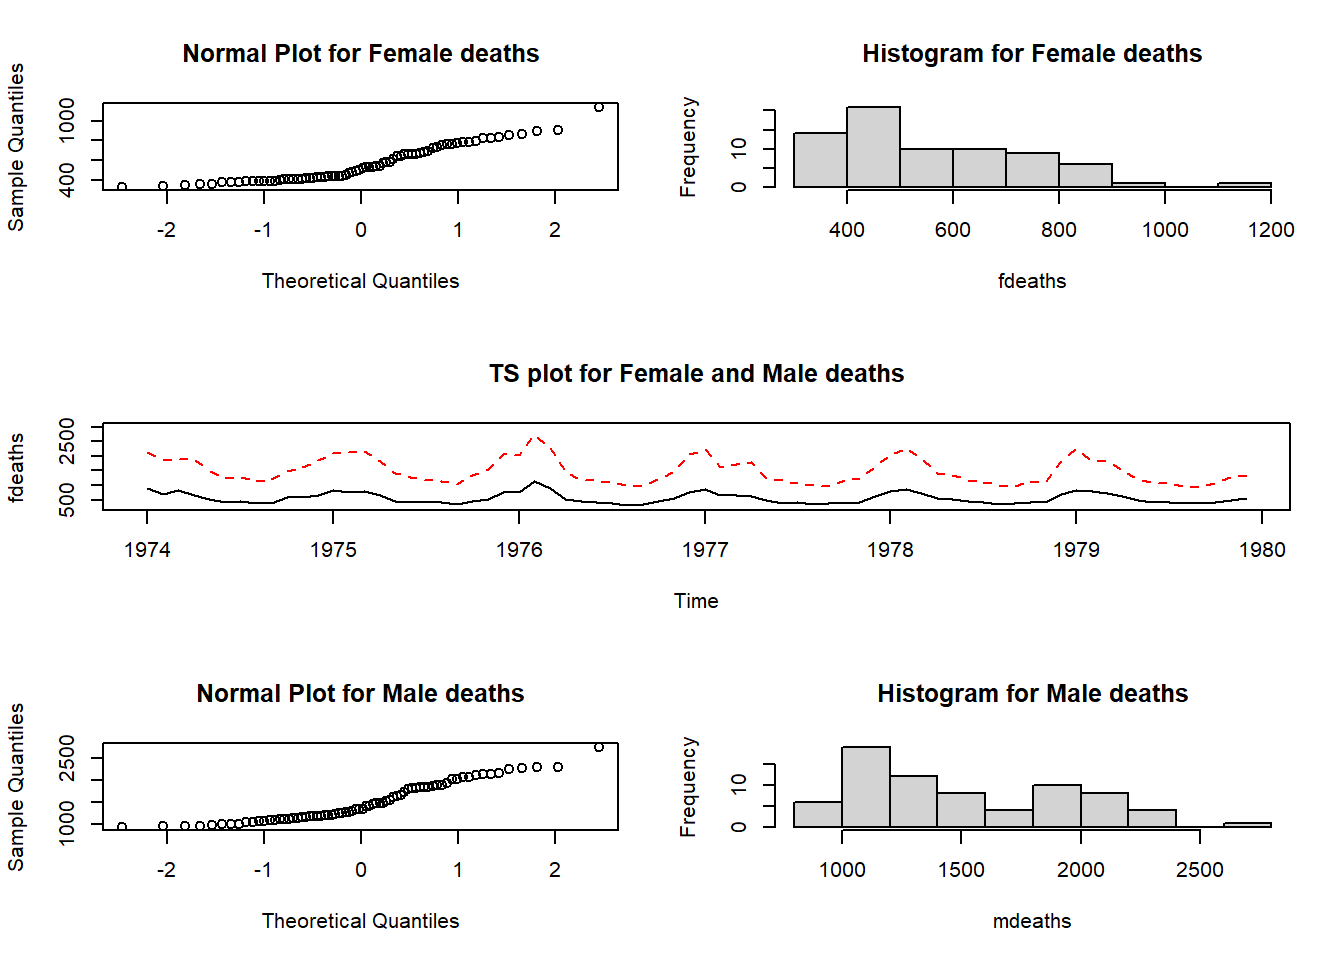
\includegraphics[width=1\linewidth]{10-graphics2_files/figure-latex/fmdeaths-1} \caption{Plots of the fdeaths and mdeaths data sets.}\label{fig:fmdeaths}
\end{figure}

\begin{Shaded}
\begin{Highlighting}[]
\FunctionTok{par}\NormalTok{ (}\AttributeTok{mfrow =} \FunctionTok{c}\NormalTok{(}\DecValTok{3}\NormalTok{, }\DecValTok{2}\NormalTok{), }\AttributeTok{mfg =} \FunctionTok{c}\NormalTok{(}\DecValTok{1}\NormalTok{, }\DecValTok{1}\NormalTok{))}
\end{Highlighting}
\end{Shaded}

The \texttt{mfrow} setting reserves three rows and two columns for graphics to be filled row-wise. The \texttt{mfg} setting specifies that the next graph will be placed in the position defined by row one column one. Once this graph has been constructed the instruction

\begin{Shaded}
\begin{Highlighting}[]
\FunctionTok{par}\NormalTok{ (}\AttributeTok{mfg =} \FunctionTok{c}\NormalTok{(}\DecValTok{1}\NormalTok{, }\DecValTok{2}\NormalTok{))}
\end{Highlighting}
\end{Shaded}

will result in the next graph to appear in the position defined by row one and column two. Next we need the instruction

\begin{Shaded}
\begin{Highlighting}[]
\FunctionTok{par}\NormalTok{ (}\AttributeTok{mfrow =} \FunctionTok{c}\NormalTok{(}\DecValTok{3}\NormalTok{, }\DecValTok{1}\NormalTok{), }\AttributeTok{mfg =} \FunctionTok{c}\NormalTok{(}\DecValTok{2}\NormalTok{, }\DecValTok{1}\NormalTok{))}
\end{Highlighting}
\end{Shaded}

requesting a graph window having three rows and one column with the next graph to appear at position row two (only one column in row two).

\begin{enumerate}
\def\labelenumi{(\alph{enumi})}
\setcounter{enumi}{2}
\item
  Note how the meaning of the margins changes when more than one figure is drawn on a page to make provision for an \emph{{outer margin}} surrounding all figures in addition to the \emph{{margin}} surrounding each separate figure.
\item
  Study how the functions \texttt{split.screen()}, \texttt{screen()} and \texttt{close.screen()} work as explained in the help facility.
\item
  Study the usage of the function \texttt{layout()} in detail for more complicated arrangements of the graph window. An example of its usage is deferred until later in the chapter.
\end{enumerate}

\section{Low-level plotting commands}\label{low-level-plotting-commands}

\begin{itemize}
\tightlist
\item
  The functions in Table \ref{tab:lowlevelPlotFuncs} are used to edit existing graphs.\\
\item
  Study these functions carefully.
\item
  Study how the right mouse button is used with R graphs.
\item
  Most plotting tasks require some combination of high-level and low-level plotting commands.
\end{itemize}

\begin{longtable}[]{@{}
  >{\raggedright\arraybackslash}p{(\linewidth - 2\tabcolsep) * \real{0.2857}}
  >{\raggedright\arraybackslash}p{(\linewidth - 2\tabcolsep) * \real{0.7143}}@{}}
\caption{\label{tab:lowlevelPlotFuncs} Low-level plotting functions.}\tabularnewline
\toprule\noalign{}
\begin{minipage}[b]{\linewidth}\raggedright
\emph{{Function}}
\end{minipage} & \begin{minipage}[b]{\linewidth}\raggedright
\emph{{Description}}
\end{minipage} \\
\midrule\noalign{}
\endfirsthead
\toprule\noalign{}
\begin{minipage}[b]{\linewidth}\raggedright
\emph{{Function}}
\end{minipage} & \begin{minipage}[b]{\linewidth}\raggedright
\emph{{Description}}
\end{minipage} \\
\midrule\noalign{}
\endhead
\bottomrule\noalign{}
\endlastfoot
\texttt{abline()} & Add regression lines to a plot; Also for adding a vertical and horizontal lines to a plot \\
\texttt{arrows()} & Draw arrow on plot \\
\texttt{axis()} & Add custom axis to plot \\
\texttt{box()} & Draw box around plot \\
\texttt{chull()} & Compute a convex hull \\
\texttt{jitter()} & Add a small amount of noise \\
\texttt{legend()} & Add a legend to a plot \\
\texttt{lines()} & Add lines to a plot \\
\texttt{mtext()} & Write text in margins \\
\texttt{points()} & Add points to a plot \\
\texttt{polygon()} & Draw and shade polygons \\
\texttt{rug()} & Add data-based marks to an axis \\
\texttt{segments()} & Draw disconnected line segments \\
\texttt{symbols()} & Draw symbols on a plot \\
\texttt{text()} & Add text to a plot \\
\texttt{title()} & Add titles or axis labels to a plot \\
\end{longtable}

\section{Using the plotting commands}\label{using-the-plotting-commands}

\subsection{Multiple lines or groups of points on the same graph}\label{matplot}

Study how the function \texttt{matplot()} works. Note the functions \texttt{matlines()} and \texttt{matpoints()}. Study and execute the following example:

\begin{Shaded}
\begin{Highlighting}[]
\NormalTok{my.func }\OtherTok{\textless{}{-}} \ControlFlowTok{function}\NormalTok{ () }
\NormalTok{\{ times }\OtherTok{\textless{}{-}} \FunctionTok{matrix}\NormalTok{(}\DecValTok{0}\NormalTok{,}\DecValTok{100}\NormalTok{,}\DecValTok{3}\NormalTok{)}
  \ControlFlowTok{for}\NormalTok{(i }\ControlFlowTok{in} \DecValTok{1}\SpecialCharTok{:}\DecValTok{100}\NormalTok{)}
\NormalTok{    \{  n }\OtherTok{\textless{}{-}}\NormalTok{ i }\SpecialCharTok{*} \DecValTok{10000}
\NormalTok{       s1 }\OtherTok{\textless{}{-}} \DecValTok{1}\SpecialCharTok{:}\NormalTok{n}
\NormalTok{       s2 }\OtherTok{\textless{}{-}} \FunctionTok{sample}\NormalTok{(n)}
\NormalTok{       s3 }\OtherTok{\textless{}{-}} \FunctionTok{rnorm}\NormalTok{(n)}
\NormalTok{       times[i,}\DecValTok{1}\NormalTok{] }\OtherTok{\textless{}{-}} \FunctionTok{system.time}\NormalTok{(}\FunctionTok{sort}\NormalTok{(s1))[}\DecValTok{1}\NormalTok{]}
\NormalTok{       times[i,}\DecValTok{2}\NormalTok{] }\OtherTok{\textless{}{-}} \FunctionTok{system.time}\NormalTok{(}\FunctionTok{sort}\NormalTok{(s2))[}\DecValTok{1}\NormalTok{]}
\NormalTok{       times[i,}\DecValTok{3}\NormalTok{] }\OtherTok{\textless{}{-}} \FunctionTok{system.time}\NormalTok{(}\FunctionTok{sort}\NormalTok{(s3))[}\DecValTok{1}\NormalTok{]}
\NormalTok{     \}}
  \FunctionTok{matplot}\NormalTok{(}\AttributeTok{x =}\NormalTok{ (}\DecValTok{1}\SpecialCharTok{:}\DecValTok{100}\NormalTok{)}\SpecialCharTok{*}\DecValTok{10000}\NormalTok{, }\AttributeTok{y=}\NormalTok{ times, }\AttributeTok{type =} \StringTok{"l"}\NormalTok{, }\AttributeTok{lty =} \DecValTok{1}\SpecialCharTok{:}\DecValTok{3}\NormalTok{,}
          \AttributeTok{col =} \FunctionTok{c}\NormalTok{(}\StringTok{"black"}\NormalTok{, }\StringTok{"green"}\NormalTok{, }\StringTok{"red"}\NormalTok{), }\AttributeTok{xlab =} \StringTok{"Length"}\NormalTok{,  }
          \AttributeTok{ylab =} \StringTok{"Time in seconds"}\NormalTok{, }\AttributeTok{main =} \StringTok{"Time for sorting"}\NormalTok{)  }
\NormalTok{\}}
\FunctionTok{my.func}\NormalTok{()}
\end{Highlighting}
\end{Shaded}

\begin{figure}
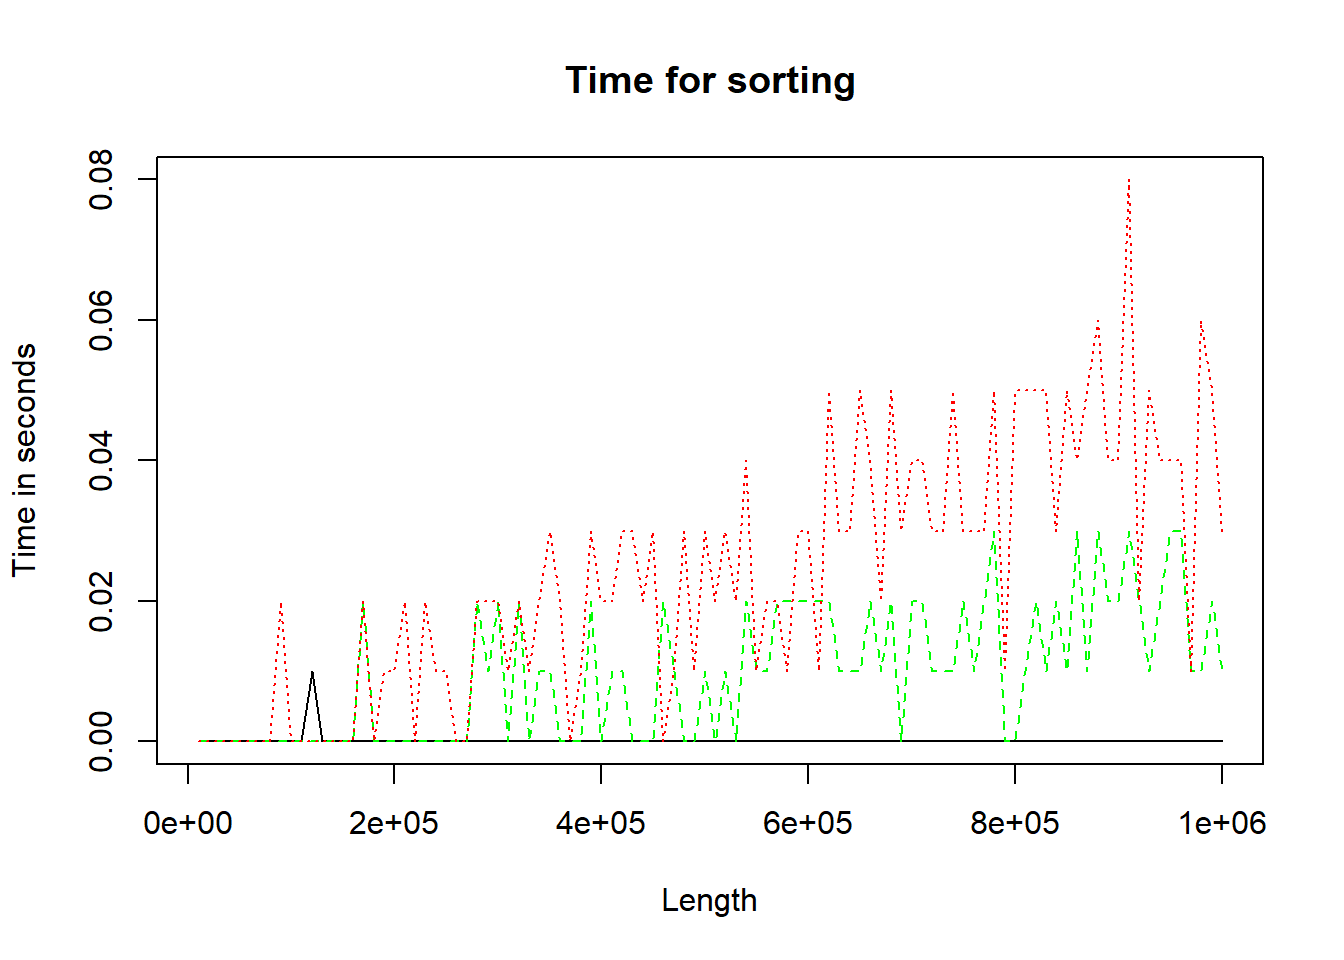
\includegraphics[width=1\linewidth]{10-graphics2_files/figure-latex/matplotExample-1} \caption{Three methods of performing sort.}\label{fig:matplotExample}
\end{figure}

\subsection{Multiple lines or groups of points on the same graph but the lines (points) are not all the same length (number)}\label{multipleLines}

What technique must be followed? First study the \texttt{Cars93} data set in package \texttt{MASS}; then study and execute the code below. Experiment with different values of \texttt{spar}.

\begin{Shaded}
\begin{Highlighting}[]
\NormalTok{my.func }\OtherTok{\textless{}{-}} \ControlFlowTok{function}\NormalTok{ (}\AttributeTok{spar =} \FloatTok{0.9}\NormalTok{)}
\NormalTok{\{ }\FunctionTok{require}\NormalTok{ (MASS)                             }\CommentTok{\# What is the effect of require()?}
\NormalTok{  oldstate }\OtherTok{\textless{}{-}} \FunctionTok{par}\NormalTok{ (}\AttributeTok{no.readonly =} \ConstantTok{TRUE}\NormalTok{)       }\CommentTok{\# Describe object \textquotesingle{}oldstate\textquotesingle{}}
  \FunctionTok{on.exit}\NormalTok{ (}\FunctionTok{par}\NormalTok{ (oldstate))                   }\CommentTok{\# Of what use is on.exit()?}
  \FunctionTok{par}\NormalTok{ (}\AttributeTok{mfrow =} \FunctionTok{c}\NormalTok{(}\DecValTok{1}\NormalTok{,}\DecValTok{2}\NormalTok{))}
  
\NormalTok{  cargrp }\OtherTok{\textless{}{-}}\NormalTok{ Cars93[ , }\StringTok{"Type"}\NormalTok{]}
\NormalTok{  price }\OtherTok{\textless{}{-}}\NormalTok{ Cars93[ , }\StringTok{"Price"}\NormalTok{]}
\NormalTok{  mpg.city }\OtherTok{\textless{}{-}}\NormalTok{ Cars93[ , }\StringTok{"MPG.city"}\NormalTok{]}
\NormalTok{  mpg.highway }\OtherTok{\textless{}{-}}\NormalTok{ Cars93[ , }\StringTok{"MPG.highway"}\NormalTok{]}
  \FunctionTok{plot}\NormalTok{(price, mpg.city, }\AttributeTok{type =} \StringTok{"n"}\NormalTok{, }\AttributeTok{ylim =} \FunctionTok{c}\NormalTok{(}\DecValTok{0}\NormalTok{, }\FunctionTok{max}\NormalTok{(mpg.city)), }
       \AttributeTok{main =} \StringTok{"Fuel Con. vs Price for City"}\NormalTok{, }\AttributeTok{xlab =} \StringTok{"Price"}\NormalTok{, }
       \AttributeTok{ylab =} \StringTok{"Miles per Gallon in City"}\NormalTok{)}
\NormalTok{  jj }\OtherTok{\textless{}{-}} \DecValTok{0}
  \ControlFlowTok{for}\NormalTok{(i }\ControlFlowTok{in} \FunctionTok{levels}\NormalTok{(cargrp))}
\NormalTok{    \{  jj }\OtherTok{\textless{}{-}}\NormalTok{ jj}\SpecialCharTok{+}\DecValTok{1}
       \FunctionTok{lines}\NormalTok{ (}\FunctionTok{smooth.spline}\NormalTok{ (price[cargrp}\SpecialCharTok{==}\NormalTok{i], mpg.city[cargrp}\SpecialCharTok{==}\NormalTok{i], }\AttributeTok{spar=}\NormalTok{spar),}
              \AttributeTok{lty =}\NormalTok{ jj, }\AttributeTok{col =}\NormalTok{ jj, }\AttributeTok{lwd=}\DecValTok{2}\NormalTok{)}
\NormalTok{    \}}
  \FunctionTok{plot}\NormalTok{(price, mpg.highway, }\AttributeTok{type =} \StringTok{"n"}\NormalTok{, }\AttributeTok{ylim =} \FunctionTok{c}\NormalTok{(}\DecValTok{0}\NormalTok{, }\FunctionTok{max}\NormalTok{(mpg.highway)), }
       \AttributeTok{main =} \StringTok{"Fuel Con. vs Price for Highway"}\NormalTok{, }\AttributeTok{xlab =} \StringTok{"Price"}\NormalTok{, }
       \AttributeTok{ylab =} \StringTok{"Miles per Gallon on Highway"}\NormalTok{)}
\NormalTok{  jj }\OtherTok{\textless{}{-}} \DecValTok{0}
  \ControlFlowTok{for}\NormalTok{(i }\ControlFlowTok{in} \FunctionTok{levels}\NormalTok{(cargrp))}
\NormalTok{    \{  jj }\OtherTok{\textless{}{-}}\NormalTok{ jj}\SpecialCharTok{+}\DecValTok{1}
       \FunctionTok{lines}\NormalTok{ (}\FunctionTok{smooth.spline}\NormalTok{ (price[cargrp}\SpecialCharTok{==}\NormalTok{i], mpg.highway[cargrp}\SpecialCharTok{==}\NormalTok{i], }
                             \AttributeTok{spar =}\NormalTok{ spar),}
              \AttributeTok{lty =}\NormalTok{ jj, }\AttributeTok{col =}\NormalTok{ jj, }\AttributeTok{lwd =} \DecValTok{2}\NormalTok{)}
\NormalTok{    \}}
\NormalTok{\}}
\FunctionTok{my.func}\NormalTok{()}
\CommentTok{\#\textgreater{} Loading required package: MASS}
\end{Highlighting}
\end{Shaded}

\begin{figure}
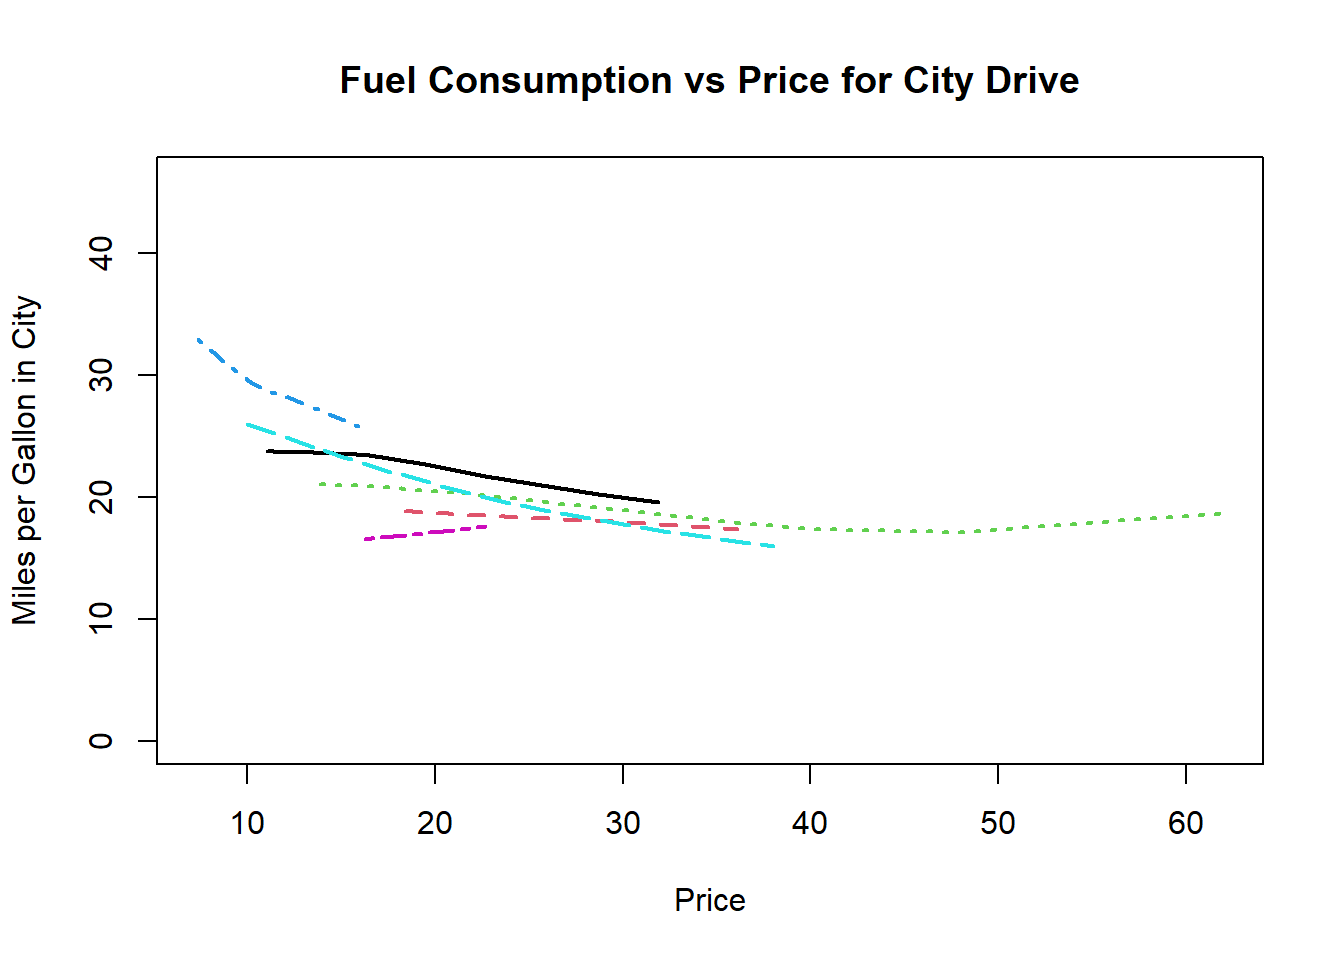
\includegraphics[width=1\linewidth]{10-graphics2_files/figure-latex/diffLengths-1} \caption{Plotting multiple lines of different lenghts}\label{fig:diffLengths}
\end{figure}

\begin{enumerate}
\def\labelenumi{(\alph{enumi})}
\item
  Explain the output generated by the above function call.
\item
  What technique can also be followed in the case of point diagrams?
\end{enumerate}

\subsection{Adding legends to a graph}\label{Legends}

\begin{enumerate}
\def\labelenumi{(\alph{enumi})}
\item
  Study how the function \texttt{legend()} and the graphical parameter \texttt{usr} work. Study the code used to obtain Figure \ref{fig:cargrps}. Revise the \texttt{locator()} function.
\item
  Use the facts that one USA gallon of liquid is equal to \(0.83267\) UK (imperial) gallon of liquid and one mile is equal to \(1.6093\) kilometres to obtain a figure similar to Figure \ref{fig:diffLengths} but with a kilometres per litre scale on the right-hand side that corresponds to the miles per gallon (USA) on highway scale on the left-hand side.
\end{enumerate}

\begin{Shaded}
\begin{Highlighting}[]
\NormalTok{my.func }\OtherTok{\textless{}{-}} \ControlFlowTok{function}\NormalTok{()}
\NormalTok{\{ }\FunctionTok{require}\NormalTok{ (MASS)  }
\NormalTok{  oldstate }\OtherTok{\textless{}{-}} \FunctionTok{par}\NormalTok{ (}\AttributeTok{no.readonly =} \ConstantTok{TRUE}\NormalTok{) }
  \FunctionTok{on.exit}\NormalTok{ (}\FunctionTok{par}\NormalTok{ (oldstate)) }

\NormalTok{  cargrp }\OtherTok{\textless{}{-}}\NormalTok{ Cars93[ , }\StringTok{"Type"}\NormalTok{]}
\NormalTok{  price }\OtherTok{\textless{}{-}}\NormalTok{ Cars93[ , }\StringTok{"Price"}\NormalTok{]}
\NormalTok{  mpg.city }\OtherTok{\textless{}{-}}\NormalTok{ Cars93[ , }\StringTok{"MPG.city"}\NormalTok{]}
  \FunctionTok{plot}\NormalTok{(price, mpg.city, }\AttributeTok{type =} \StringTok{"n"}\NormalTok{, }\AttributeTok{ylim =} \FunctionTok{c}\NormalTok{(}\DecValTok{0}\NormalTok{, }\FunctionTok{max}\NormalTok{(mpg.city)), }
       \AttributeTok{main =} \StringTok{"Fuel Consumption vs Price for City Drive"}\NormalTok{, }\AttributeTok{xlab =} \StringTok{"Price"}\NormalTok{, }
       \AttributeTok{ylab =} \StringTok{"Miles per Gallon in City"}\NormalTok{)}
\NormalTok{  char }\OtherTok{\textless{}{-}} \FunctionTok{substring}\NormalTok{ (}\FunctionTok{as.character}\NormalTok{ (cargrp), }\DecValTok{1}\NormalTok{, }\DecValTok{2}\NormalTok{)}
  \FunctionTok{text}\NormalTok{ (}\AttributeTok{x =}\NormalTok{ price, }\AttributeTok{y =}\NormalTok{ mpg.city, }\AttributeTok{labels =}\NormalTok{ char, }\AttributeTok{pos =} \DecValTok{1}\NormalTok{, }\AttributeTok{cex =} \FloatTok{0.75}\NormalTok{)}
\NormalTok{  labs }\OtherTok{\textless{}{-}} \FunctionTok{paste}\NormalTok{ (}\FunctionTok{substring}\NormalTok{ (}\FunctionTok{levels}\NormalTok{ (cargrp), }\DecValTok{1}\NormalTok{, }\DecValTok{2}\NormalTok{), }\FunctionTok{levels}\NormalTok{(cargrp), }\AttributeTok{sep=}\StringTok{":  "}\NormalTok{)}
  \FunctionTok{legend}\NormalTok{(}\AttributeTok{x =} \DecValTok{40}\NormalTok{, }\AttributeTok{y =} \DecValTok{42}\NormalTok{, }\AttributeTok{legend =}\NormalTok{ labs)}
\NormalTok{\}}
\FunctionTok{my.func}\NormalTok{ ()}
\end{Highlighting}
\end{Shaded}

\begin{figure}
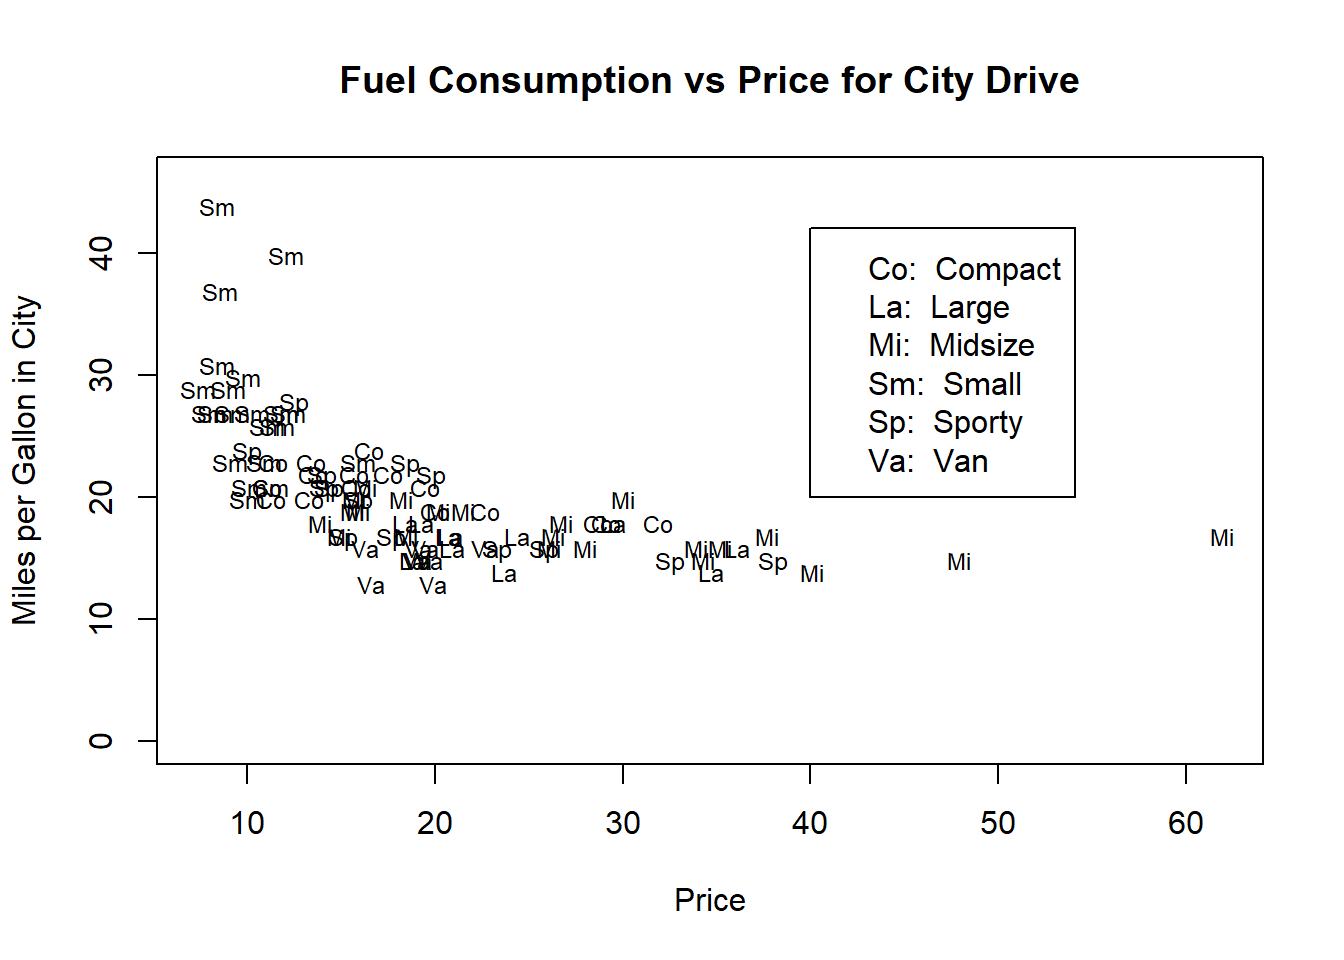
\includegraphics[width=1\linewidth]{10-graphics2_files/figure-latex/cargrps-1} \caption{Illustrating adding a legend to a plot.}\label{fig:cargrps}
\end{figure}

\subsection{Multiple plots with identical axes}\label{multAxes}

How can various graphs with identical axes be obtained? Show how this can be done by graphing the sorting time for the three procedures considered in section \ref{matplot} above in three separate plots in the same graph window.

\subsection{Providing a single legend for multiple plots}\label{providing-a-single-legend-for-multiple-plots}

Suppose there were two sorting methods for each of the three situations described in\ref{matplot} and \ref{multAxes} above. How can the three graphs be provided with a single legend without the legend appearing in one of the graphs? Explain in detail.

\subsection{Changing the plotting character: common plotting characters in R}\label{changing-the-plotting-character-common-plotting-characters-in-r}

Note the use of graphical parameters \texttt{pch} and \texttt{mkh}. What plotting characters are available? Study the help file of \texttt{par()} and \texttt{points()}. Study the plotting characters displayed in Figure \ref{fig:pch} and the code used to produce the figure. How can plotting characters be made to appear in legends?

\begin{Shaded}
\begin{Highlighting}[]
\FunctionTok{plot}\NormalTok{ (}\AttributeTok{x =} \FunctionTok{rep}\NormalTok{(}\DecValTok{1}\SpecialCharTok{:}\DecValTok{10}\NormalTok{, }\DecValTok{2}\NormalTok{), }\AttributeTok{y =} \FunctionTok{rep}\NormalTok{ (}\FunctionTok{c}\NormalTok{(}\DecValTok{1}\NormalTok{,}\DecValTok{2}\NormalTok{), }\FunctionTok{c}\NormalTok{(}\DecValTok{10}\NormalTok{,}\DecValTok{10}\NormalTok{)), }\AttributeTok{pch =} \DecValTok{0}\SpecialCharTok{:}\DecValTok{19}\NormalTok{, }\AttributeTok{cex =} \DecValTok{2}\NormalTok{, }
      \AttributeTok{pty =} \StringTok{"p"}\NormalTok{, }\AttributeTok{ylim =} \FunctionTok{c}\NormalTok{(}\DecValTok{0}\NormalTok{,}\DecValTok{3}\NormalTok{), }\AttributeTok{xlab =} \StringTok{""}\NormalTok{, }\AttributeTok{ylab =} \StringTok{""}\NormalTok{, }\AttributeTok{xaxt =} \StringTok{"n"}\NormalTok{, }\AttributeTok{yaxt =} \StringTok{"n"}\NormalTok{)}
\end{Highlighting}
\end{Shaded}

\begin{figure}
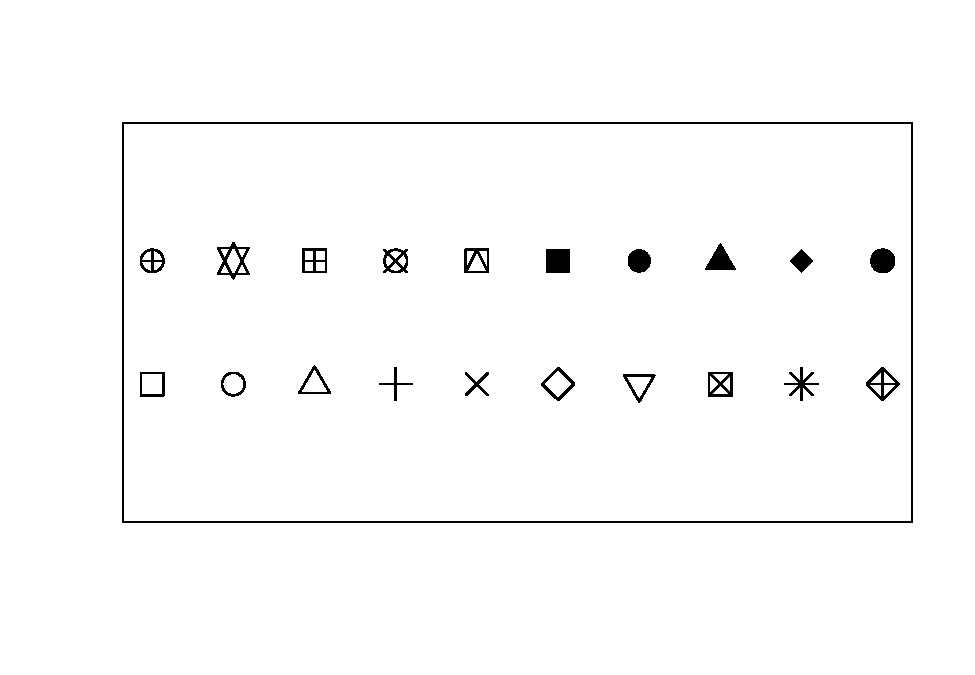
\includegraphics[width=1\linewidth]{10-graphics2_files/figure-latex/pch-1} \caption{Some common plotting characters available in R.}\label{fig:pch}
\end{figure}

\subsection{Changing the colour in plots}\label{changing-the-colour-in-plots}

The graphical parameter \texttt{col} allows the user to specify the colour(s) in number format as given in Figure \ref{fig:col}. The full list of named colours can be obtained with the command \texttt{colors()} in the Console.

Alternatively, the colour can be specified by hue, saturation and value with \texttt{hsv\ (h\ =\ ,\ s\ =\ ,\ v\ =\ )}, hue, chroma and luminance with \texttt{hcl\ (h\ =\ ,\ c\ =\ ,\ l\ =\ )} or red, green and blue with \texttt{rgb\ (red\ =\ ,\ green\ =\ ,\ blue\ =\ )}. The \texttt{rgb()} function has an argument \texttt{maxColorValue} with default value \texttt{1} which indicates the range known as the gamma-compressed values. Typically, the red, green and blue values range between 0 and 255 or video display or 8-bit graphics. To select a specific shade of light blue, the following command can be used:

\begin{Shaded}
\begin{Highlighting}[]
\FunctionTok{plot}\NormalTok{ (ldeaths, }\AttributeTok{col =} \FunctionTok{rgb}\NormalTok{ (}\AttributeTok{red =} \DecValTok{167}\NormalTok{, }\AttributeTok{green =} \DecValTok{227}\NormalTok{, }\AttributeTok{blue =} \DecValTok{227}\NormalTok{, }
                          \AttributeTok{maxColorValue =} \DecValTok{255}\NormalTok{))}
\end{Highlighting}
\end{Shaded}

\begin{figure}
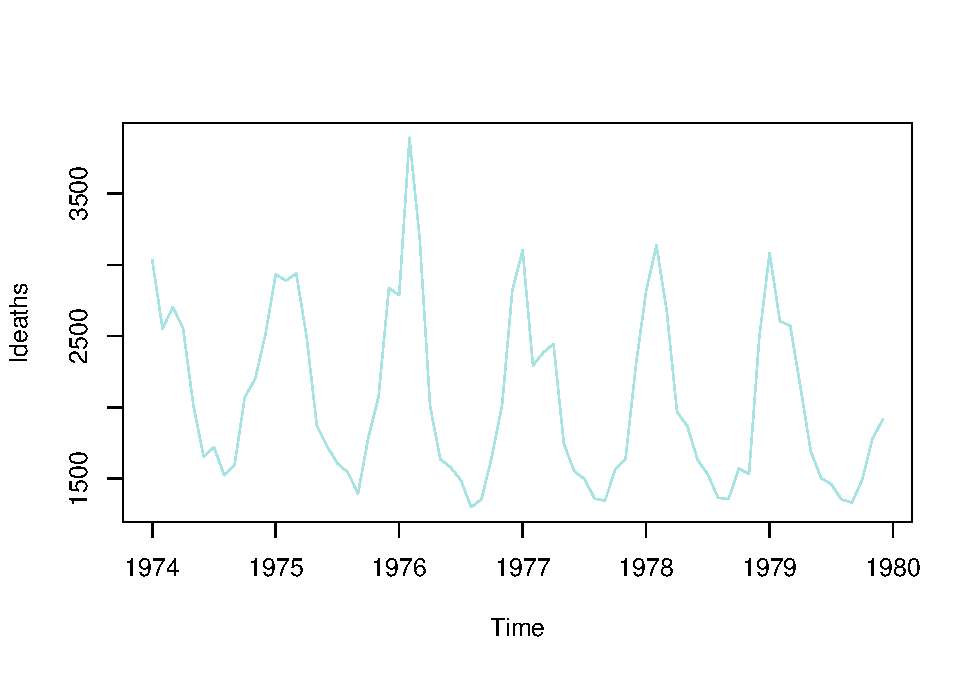
\includegraphics[width=1\linewidth]{10-graphics2_files/figure-latex/colExample-1} \caption{Colour selection with rgb().}\label{fig:colExample}
\end{figure}

The output of the \texttt{rgb()} function is in the hexidemical colour number format, e.g.~``\#A7E3E3''. The function \texttt{col2rgb()} accepts a colour name, hexadecimal colour number format or colour number and provides the red, green and blue values in the 0 to 255 range.

\begin{figure}
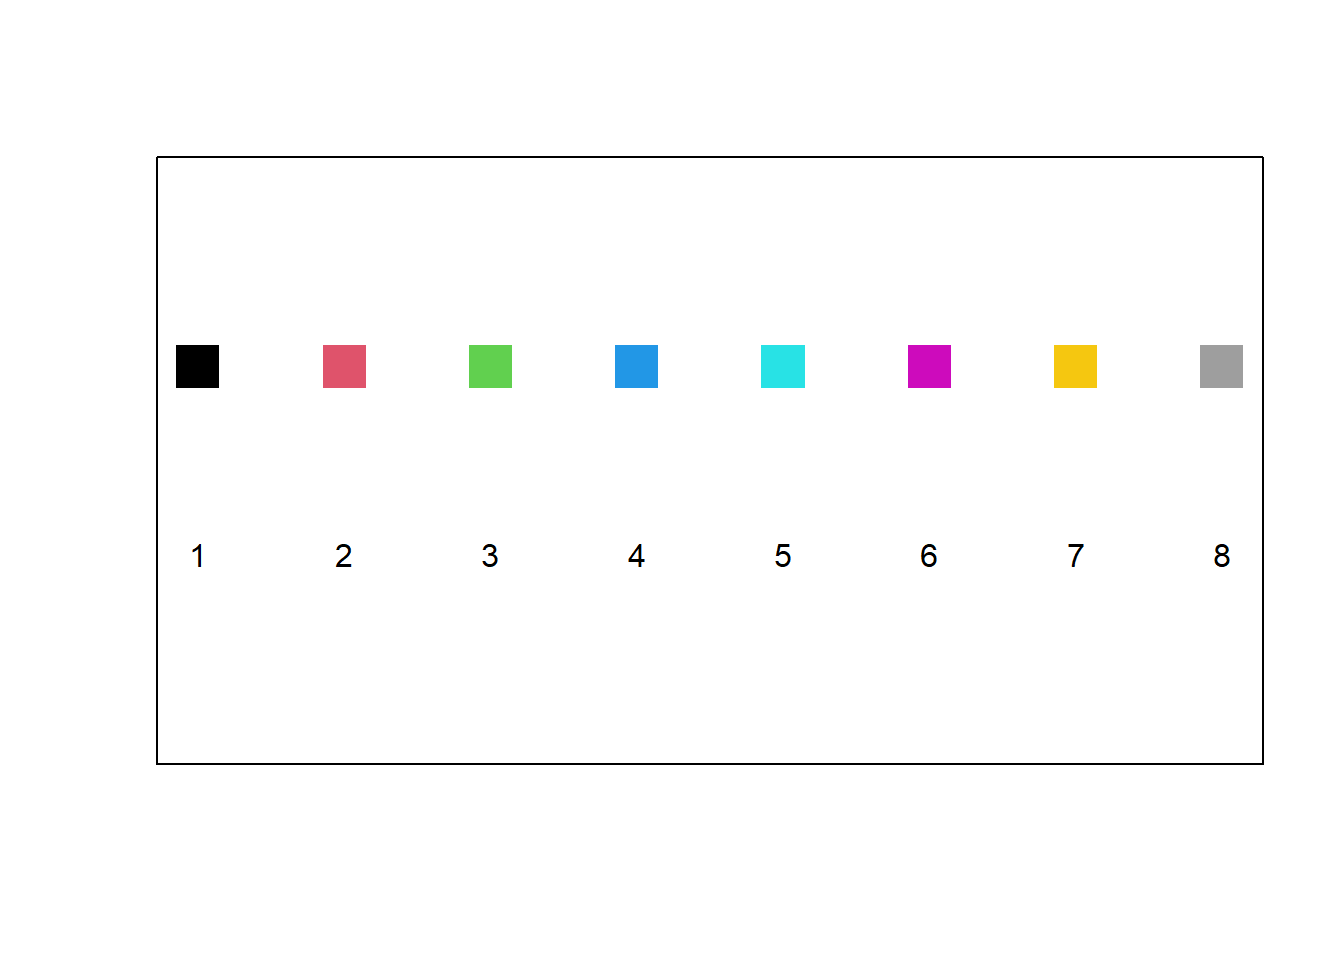
\includegraphics[width=1\linewidth]{10-graphics2_files/figure-latex/col-1} \caption{The default colour palette available in R.}\label{fig:col}
\end{figure}

A sequence of \(n\) colours can be generated with the function \texttt{colorRampPalette()}. As an example, the colour vector used for plotting in Figure \ref{fig:colRamp} were generated with the call \texttt{colorRampPalette\ (c\ ("red",\ "green",\ "white",\ "gold"))(20)}. Study how the following instructions generate colour sequences: \texttt{rainbow()}, \texttt{heat.colors()}, \texttt{terrain.colors()}, \texttt{topo.colors()}, \texttt{cm.colors()}.

\begin{figure}
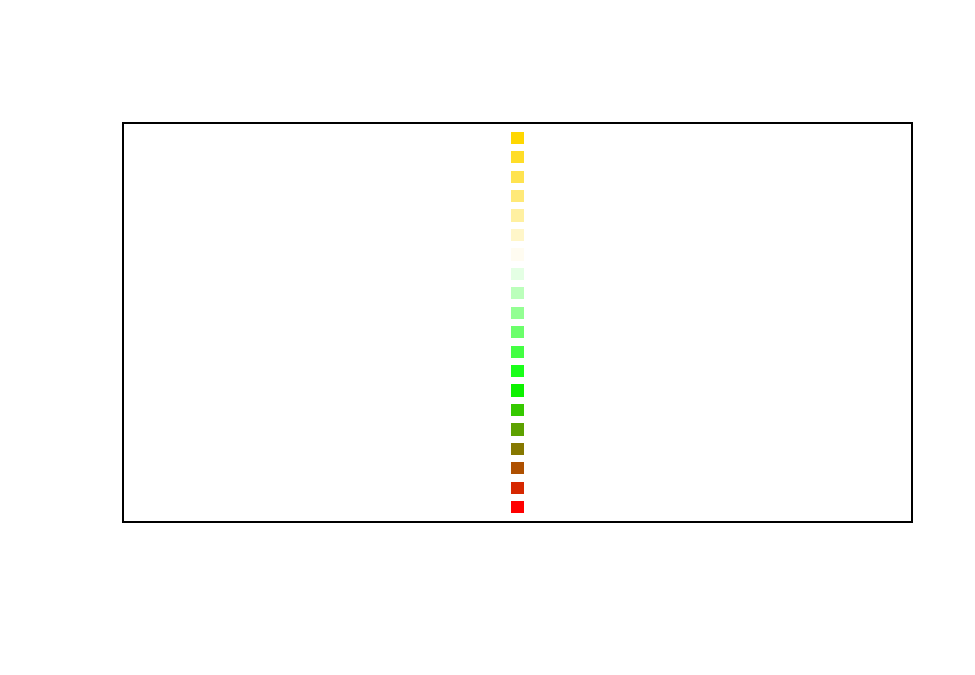
\includegraphics[width=1\linewidth]{10-graphics2_files/figure-latex/colRamp-1} \caption{User specified colour sequence with colorRampPalette().}\label{fig:colRamp}
\end{figure}

\subsection{Logarithmic axes}\label{logarithmic-axes}

The \texttt{log()} function and the \texttt{log} argument of the \texttt{plot()} function are useful in this regard. The \texttt{log} argument of the \texttt{plot()} function can be specified as \texttt{log="x"}; or \texttt{log="y"}; or \texttt{log="xy"} depending on whether the x-axis, the y-axis, or both axes should be plotted logarithmically.

\subsection{Graphs with character strings as the `scale' on the axis}\label{graphs-with-character-strings-as-the-scale-on-the-axis}

Figure \ref{fig:catAxis} illustrates how user defined character strings can appear as calibrations on an axis. Furthermore, this figure illustrates several techniques to fine-tune plots. Study the code resulting in Figure \ref{fig:catAxis} in detail.

\begin{Shaded}
\begin{Highlighting}[]
\NormalTok{my.func }\OtherTok{\textless{}{-}} \ControlFlowTok{function}\NormalTok{()}
\NormalTok{\{ old.state }\OtherTok{\textless{}{-}} \FunctionTok{par}\NormalTok{(}\AttributeTok{no.readonly =} \ConstantTok{TRUE}\NormalTok{)}
  \FunctionTok{on.exit}\NormalTok{ (}\FunctionTok{par}\NormalTok{ (old.state))}
\NormalTok{  area }\OtherTok{\textless{}{-}}\NormalTok{ state.x77[, }\StringTok{"Area"}\NormalTok{]}
\NormalTok{  income }\OtherTok{\textless{}{-}}\NormalTok{ state.x77[, }\StringTok{"Income"}\NormalTok{]}
\NormalTok{  area.grp }\OtherTok{\textless{}{-}} \FunctionTok{cut}\NormalTok{(area, }\FunctionTok{c}\NormalTok{(}\DecValTok{0}\NormalTok{, }\FunctionTok{quantile}\NormalTok{ (area, }\FunctionTok{c}\NormalTok{(}\DecValTok{1}\SpecialCharTok{/}\DecValTok{3}\NormalTok{, }\DecValTok{2}\SpecialCharTok{/}\DecValTok{3}\NormalTok{, }\DecValTok{1}\NormalTok{))),}
                  \AttributeTok{labels =} \FunctionTok{c}\NormalTok{(}\StringTok{"Small"}\NormalTok{, }\StringTok{"Medium"}\NormalTok{, }\StringTok{"Large"}\NormalTok{))}
\NormalTok{  income.grp }\OtherTok{\textless{}{-}} \FunctionTok{cut}\NormalTok{(income, }\FunctionTok{c}\NormalTok{(}\DecValTok{0}\NormalTok{, }\FunctionTok{quantile}\NormalTok{ (income, }\FunctionTok{c}\NormalTok{(}\DecValTok{1}\SpecialCharTok{/}\DecValTok{2}\NormalTok{, }\DecValTok{1}\NormalTok{))),}
                    \AttributeTok{labels =} \FunctionTok{c}\NormalTok{(}\StringTok{"Below Median"}\NormalTok{, }\StringTok{"Above Median"}\NormalTok{))}
\NormalTok{  mns }\OtherTok{\textless{}{-}} \FunctionTok{tapply}\NormalTok{(state.x77[, }\StringTok{"Illiteracy"}\NormalTok{], }\FunctionTok{list}\NormalTok{(area.grp, income.grp), mean)}
  \FunctionTok{par}\NormalTok{(}\AttributeTok{mfrow =} \FunctionTok{c}\NormalTok{(}\DecValTok{1}\NormalTok{, }\DecValTok{2}\NormalTok{))}
  \FunctionTok{plot}\NormalTok{(}\FunctionTok{c}\NormalTok{(}\FloatTok{0.8}\NormalTok{, }\FloatTok{3.2}\NormalTok{), }\FunctionTok{range}\NormalTok{(mns), }\AttributeTok{type =} \StringTok{"n"}\NormalTok{, }\AttributeTok{xaxt =} \StringTok{"n"}\NormalTok{, }\AttributeTok{xlab =} \StringTok{"Area Group"}\NormalTok{, }
       \AttributeTok{ylab =}\StringTok{"Mean Illiteracy"}\NormalTok{, }\AttributeTok{sub =} \StringTok{"Function plot() used"}\NormalTok{)}
  \FunctionTok{axis}\NormalTok{(}\AttributeTok{side =} \DecValTok{1}\NormalTok{, }\AttributeTok{at =} \DecValTok{1}\SpecialCharTok{:}\DecValTok{3}\NormalTok{, }\AttributeTok{labels =} \FunctionTok{levels}\NormalTok{(area.grp))}
  \FunctionTok{lines}\NormalTok{(}\DecValTok{1}\SpecialCharTok{:}\DecValTok{3}\NormalTok{, mns[, }\DecValTok{1}\NormalTok{])}
  \FunctionTok{lines}\NormalTok{(}\DecValTok{1}\SpecialCharTok{:}\DecValTok{3}\NormalTok{, mns[, }\DecValTok{2}\NormalTok{], }\AttributeTok{lty =} \DecValTok{2}\NormalTok{)}
  \FunctionTok{par}\NormalTok{(}\AttributeTok{usr =} \FunctionTok{c}\NormalTok{(}\DecValTok{0}\NormalTok{, }\DecValTok{1}\NormalTok{, }\DecValTok{0}\NormalTok{, }\DecValTok{1}\NormalTok{))}
  \FunctionTok{legend}\NormalTok{(}\FloatTok{0.56}\NormalTok{, }\FloatTok{0.96}\NormalTok{, }\AttributeTok{lty =} \FunctionTok{c}\NormalTok{(}\DecValTok{1}\NormalTok{,}\DecValTok{2}\NormalTok{), }\AttributeTok{legend =} \FunctionTok{levels}\NormalTok{(income.grp), }\AttributeTok{cex=} \FloatTok{0.5}\NormalTok{)}
  \FunctionTok{text}\NormalTok{(}\FloatTok{0.63}\NormalTok{, }\FloatTok{0.98}\NormalTok{, }\AttributeTok{adj =} \DecValTok{0}\NormalTok{, }\StringTok{"Income Group"}\NormalTok{, }\AttributeTok{cex =} \FloatTok{0.5}\NormalTok{)}
    \FunctionTok{interaction.plot}\NormalTok{(area.grp, income.grp, state.x77[,}\StringTok{"Illiteracy"}\NormalTok{], }
                     \AttributeTok{xlab =} \StringTok{"Area Group"}\NormalTok{, }\AttributeTok{ylab =} \StringTok{"Mean Illiteracy"}\NormalTok{, }
                     \AttributeTok{sub =} \StringTok{"Interaction.plot used"}\NormalTok{, }\AttributeTok{lty =} \DecValTok{1}\SpecialCharTok{:}\DecValTok{2}\NormalTok{, }\AttributeTok{xtick =} \ConstantTok{TRUE}\NormalTok{, }
                     \AttributeTok{legend =} \ConstantTok{FALSE}\NormalTok{)}
  \FunctionTok{par}\NormalTok{(}\AttributeTok{mfrow =} \FunctionTok{c}\NormalTok{(}\DecValTok{1}\NormalTok{,}\DecValTok{1}\NormalTok{))}
  \FunctionTok{par}\NormalTok{(}\AttributeTok{new =}\NormalTok{ T)}
  \FunctionTok{plot}\NormalTok{(}\DecValTok{1}\SpecialCharTok{:}\DecValTok{10}\NormalTok{, }\DecValTok{1}\SpecialCharTok{:}\DecValTok{10}\NormalTok{, }\AttributeTok{type=}\StringTok{"n"}\NormalTok{, }\AttributeTok{xlab=}\StringTok{""}\NormalTok{, }\AttributeTok{ylab=}\StringTok{""}\NormalTok{,}\AttributeTok{axes =} \ConstantTok{FALSE}\NormalTok{)}
  \FunctionTok{title}\NormalTok{(}\AttributeTok{main =} \StringTok{"Illiteracy vs Size for States grouped by Income"}\NormalTok{)}
\NormalTok{\}}
\FunctionTok{my.func}\NormalTok{ ()}
\end{Highlighting}
\end{Shaded}

\begin{figure}
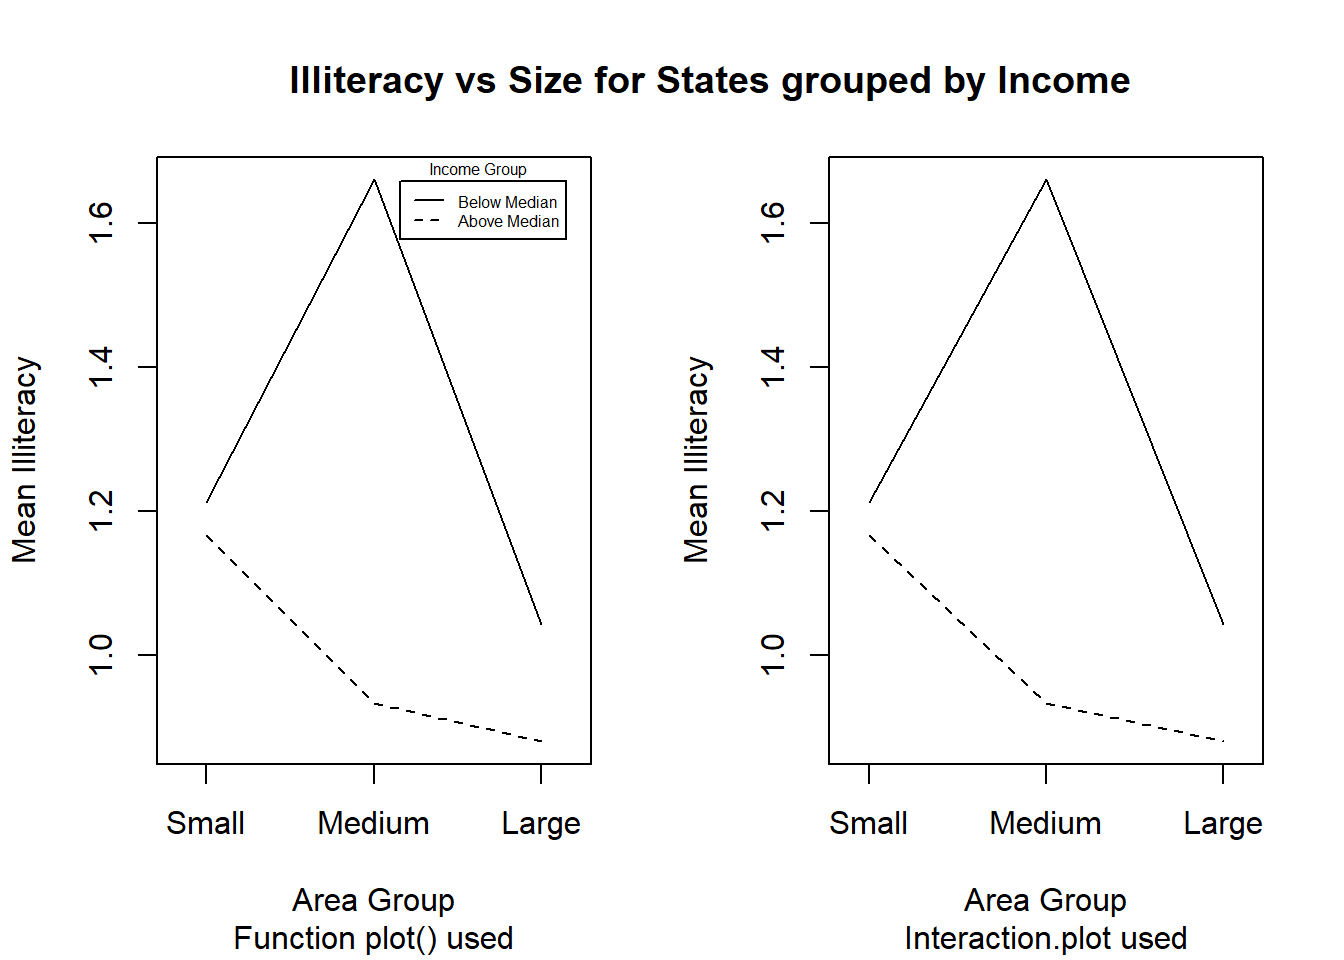
\includegraphics[width=1\linewidth]{10-graphics2_files/figure-latex/catAxis-1} \caption{Figures with character strings as axis calibrations and other enhancements to plots.}\label{fig:catAxis}
\end{figure}

\subsection{Customizing bar charts and histograms}\label{customizing-bar-charts-and-histograms}

\begin{enumerate}
\def\labelenumi{(\alph{enumi})}
\item
  How can every bar in a bar chart be represented in a different colour and be given separate headings?
\item
  How can only a line graph without any colours be obtained?
\item
  How can a probability density function be superimposed on a histogram?
\item
  How can bar charts be provided with user-defined axes?
\end{enumerate}

Use the \texttt{Cars93} data set to answer the above four questions by constructing a figure similar to the one shown in Figure \ref{fig:BarHist}. Note: In the Mean MPG plot not all car types are used. If a factor variable is subsetted the original levels will be kept although some of them might not occurr. Hence it might be necessary to create a new factor variable with only the levels that are needed by using \texttt{factor()}.

\begin{figure}
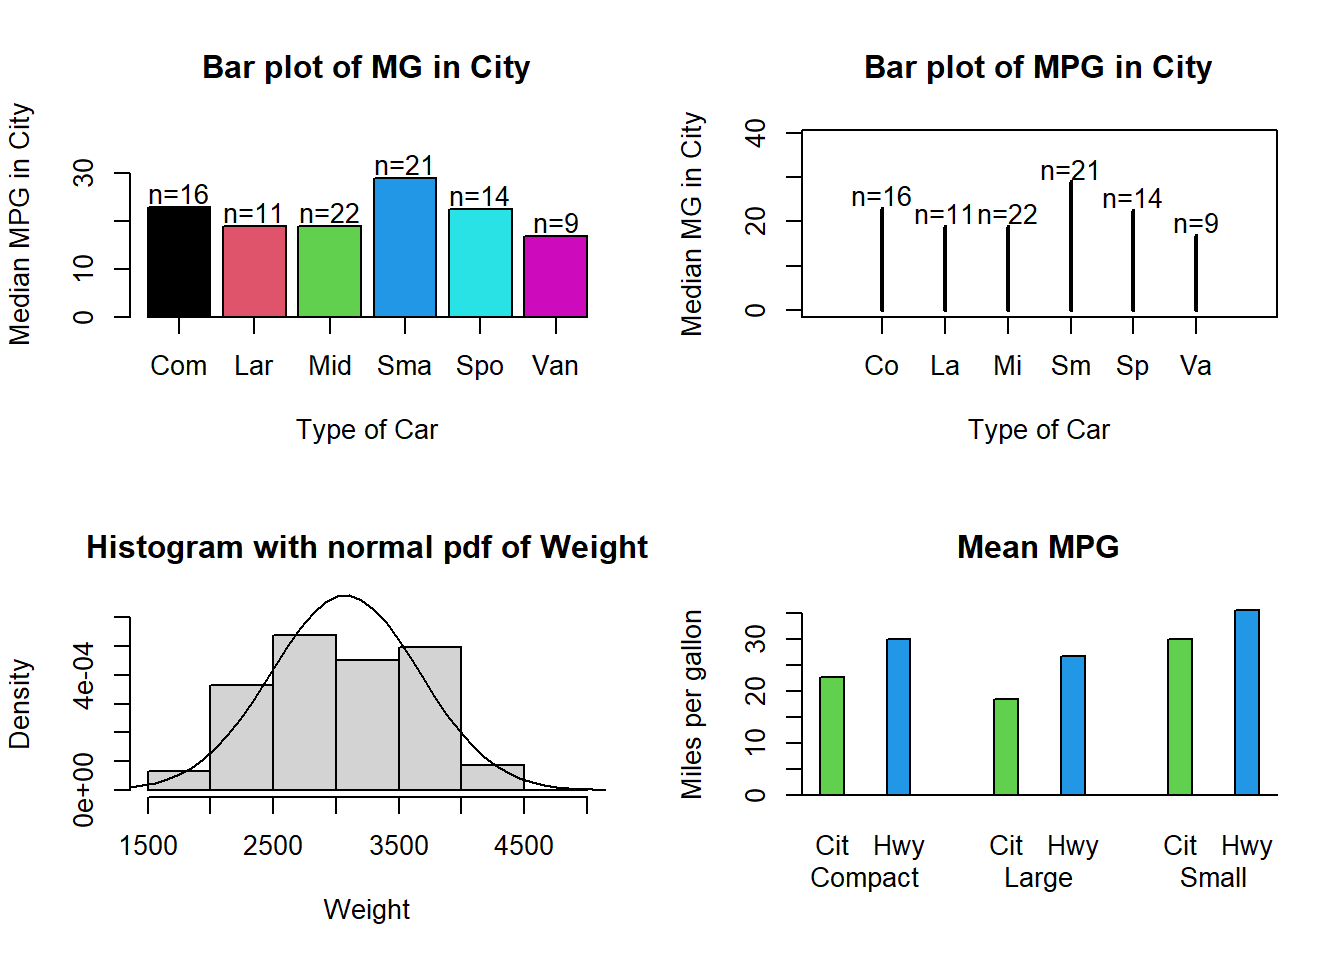
\includegraphics[width=1\linewidth]{10-graphics2_files/figure-latex/BarHist-1} \caption{Enhanced bar charts and histograms.}\label{fig:BarHist}
\end{figure}

\subsection{Three-dimensional graphical displays}\label{three-dimensional-graphical-displays}

\begin{enumerate}
\def\labelenumi{(\alph{enumi})}
\item
  Study how the function \texttt{persp()} works.
\item
  Work through the example code that creates Figure \ref{fig:persp}. Apart from the arrow that points to the maximum, different colours must be used to highlight the different aspects of the graph.
\item
  Provide horizontally and vertically rotated views of the 3D plot.
\end{enumerate}

\begin{Shaded}
\begin{Highlighting}[]
\NormalTok{my.func }\OtherTok{\textless{}{-}} \ControlFlowTok{function}\NormalTok{ () }
\NormalTok{\{ x }\OtherTok{\textless{}{-}} \FunctionTok{seq}\NormalTok{(}\SpecialCharTok{{-}}\DecValTok{10}\NormalTok{, }\DecValTok{10}\NormalTok{, }\AttributeTok{length=} \DecValTok{30}\NormalTok{)}
\NormalTok{  y }\OtherTok{\textless{}{-}}\NormalTok{ x}
\NormalTok{  ff }\OtherTok{\textless{}{-}} \ControlFlowTok{function}\NormalTok{(x,y) \{ r }\OtherTok{\textless{}{-}} \FunctionTok{sqrt}\NormalTok{(x}\SpecialCharTok{\^{}}\DecValTok{2}\SpecialCharTok{+}\NormalTok{y}\SpecialCharTok{\^{}}\DecValTok{2}\NormalTok{); }\DecValTok{10} \SpecialCharTok{*} \FunctionTok{sin}\NormalTok{(r)}\SpecialCharTok{/}\NormalTok{r \}}
\NormalTok{  z }\OtherTok{\textless{}{-}} \FunctionTok{outer}\NormalTok{(x, y, ff)}
\NormalTok{  z[}\FunctionTok{is.na}\NormalTok{(z)] }\OtherTok{\textless{}{-}} \DecValTok{1}
\NormalTok{  op }\OtherTok{\textless{}{-}} \FunctionTok{par}\NormalTok{(}\AttributeTok{bg =} \StringTok{"white"}\NormalTok{)}
\CommentTok{\#  persp(x, y, z, theta = 30, phi = 30, expand = 0.5, col = "lightblue")}
\NormalTok{  res }\OtherTok{\textless{}{-}} \FunctionTok{persp}\NormalTok{(x, y, z, }\AttributeTok{theta =} \DecValTok{30}\NormalTok{, }\AttributeTok{phi =} \DecValTok{30}\NormalTok{, }\AttributeTok{expand =} \FloatTok{0.5}\NormalTok{, }\AttributeTok{col =} \StringTok{"lightblue"}\NormalTok{, }
               \AttributeTok{ltheta =} \DecValTok{120}\NormalTok{, }\AttributeTok{shade =} \FloatTok{0.75}\NormalTok{, }\AttributeTok{ticktype =} \StringTok{"detailed"}\NormalTok{, }\AttributeTok{xlab =} \StringTok{"X"}\NormalTok{, }
               \AttributeTok{ylab =} \StringTok{"Y"}\NormalTok{, }\AttributeTok{zlab =} \StringTok{"Z"}\NormalTok{ ) }
  \FunctionTok{print}\NormalTok{ (}\FunctionTok{round}\NormalTok{(res, }\DecValTok{3}\NormalTok{))}
  
  \CommentTok{\#{-}{-}{-} Add to existing persp plot : {-}{-}{-}}
  \CommentTok{\#{-}{-}{-} Function trans3d() {-}{-}{-}{-}{-}{-}{-}{-}{-}{-}{-}{-}{-}}
\NormalTok{    trans3d }\OtherTok{\textless{}{-}} \ControlFlowTok{function}\NormalTok{(x,y,z, pmat) }
\NormalTok{    \{}
\NormalTok{      tr }\OtherTok{\textless{}{-}} \FunctionTok{cbind}\NormalTok{(x,y,z,}\DecValTok{1}\NormalTok{) }\SpecialCharTok{\%*\%}\NormalTok{ pmat}
    \FunctionTok{list}\NormalTok{(}\AttributeTok{x =}\NormalTok{ tr[,}\DecValTok{1}\NormalTok{]}\SpecialCharTok{/}\NormalTok{tr[,}\DecValTok{4}\NormalTok{], }\AttributeTok{y =}\NormalTok{ tr[,}\DecValTok{2}\NormalTok{]}\SpecialCharTok{/}\NormalTok{tr[,}\DecValTok{4}\NormalTok{])}
\NormalTok{  \}}
  \CommentTok{\# {-}{-}{-}{-}{-}{-}{-}{-}{-}{-}{-}{-}{-}{-}{-}{-}{-}{-}{-}{-}{-}{-}{-}{-}{-}{-}{-}{-}{-}{-}{-}{-}{-}{-}}
\NormalTok{  z1 }\OtherTok{\textless{}{-}} \FunctionTok{ff}\NormalTok{(}\FloatTok{1e{-}10}\NormalTok{, }\FloatTok{1e{-}10}\NormalTok{)}
\NormalTok{  transfrm }\OtherTok{\textless{}{-}} \FunctionTok{trans3d}\NormalTok{ (}\FunctionTok{c}\NormalTok{(}\DecValTok{0}\NormalTok{,}\SpecialCharTok{{-}}\FloatTok{2.5}\NormalTok{), }\FunctionTok{c}\NormalTok{(}\DecValTok{0}\NormalTok{,}\DecValTok{5}\NormalTok{), }\FunctionTok{c}\NormalTok{(z1,z1), res)}
  \FunctionTok{arrows}\NormalTok{(transfrm}\SpecialCharTok{$}\NormalTok{x[}\DecValTok{1}\NormalTok{], transfrm}\SpecialCharTok{$}\NormalTok{y[}\DecValTok{1}\NormalTok{], transfrm}\SpecialCharTok{$}\NormalTok{x[}\DecValTok{2}\NormalTok{], transfrm}\SpecialCharTok{$}\NormalTok{y[}\DecValTok{2}\NormalTok{], }
         \AttributeTok{length =} \FloatTok{0.1}\NormalTok{, }\AttributeTok{code =} \DecValTok{1}\NormalTok{)}
  \FunctionTok{text}\NormalTok{(transfrm}\SpecialCharTok{$}\NormalTok{x[}\DecValTok{2}\NormalTok{], transfrm}\SpecialCharTok{$}\NormalTok{y[}\DecValTok{2}\NormalTok{]}\SpecialCharTok{+}\FloatTok{0.02}\NormalTok{, }\StringTok{"Maximum occurs here"}\NormalTok{)}
  \FunctionTok{return}\NormalTok{(z1)}
\NormalTok{\}}
\FunctionTok{my.func}\NormalTok{()}
\end{Highlighting}
\end{Shaded}

\begin{figure}
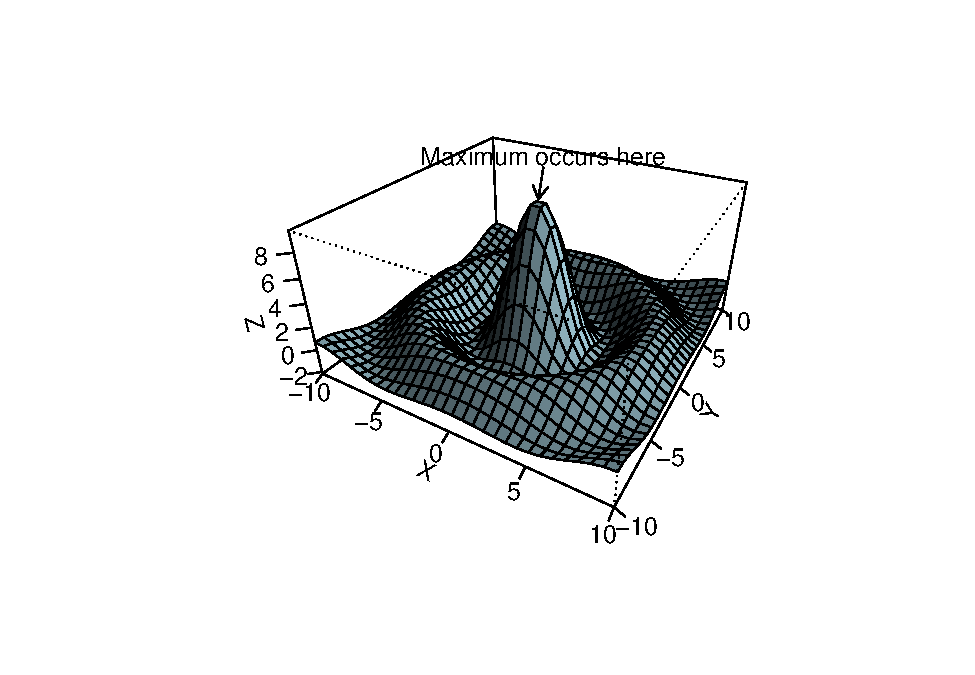
\includegraphics[width=1\linewidth]{10-graphics2_files/figure-latex/persp-1} \caption{Annotated 3D perspective plot.}\label{fig:persp}
\end{figure}

\begin{verbatim}
#>       [,1]   [,2]   [,3]   [,4]
#> [1,] 0.087 -0.025  0.043 -0.043
#> [2,] 0.050  0.043 -0.075  0.075
#> [3,] 0.000  0.074  0.042 -0.042
#> [4,] 0.000 -0.273 -2.890  3.890
#> [1] 10
\end{verbatim}

\subsection{Diagrams}\label{diagrams}

Use R to draw a simple flow diagram. The diagram must contain at least one rectangle, one square, one circle and one triangle. Furthermore, there must be straight and curved lines as well as text describing the different elements. \emph{Hint}: Study how the functions \texttt{arrows()}, \texttt{lines()}, \texttt{text()} and \texttt{symbols()} work as discussed in their respective help facilities.

\subsection{Annotating graphics with special symbols}\label{annotating-graphics-with-special-symbols}

Construct a graph of a \(normal(0, 1)\) density function. Give as a title to the plot the expression ``Density of a normal random variable with \(\mu = 0\) and \(\sigma^2 = 1\).'' \emph{Hint}: Consult the help file of \texttt{plotmath()}. Within the plot draw an arrow to the density and label it \(\frac{1}{\sqrt{2 \pi}} e^{-\frac{1}{2}x^2}\).

\section{Quantile plots}\label{qqplot}

Consider the histogram of weight in Figure \ref{fig:BarHist}. Does this variable follow a normal distribution? A normal quantile plot, shows the observations vs the corresponding quantiles of a standard normal distribution. If the observations correspond to a normal distribution, this will approximately form a straight line. Use the \texttt{qqline()} function to add a straing line to the plot.

\begin{Shaded}
\begin{Highlighting}[]
\FunctionTok{qqnorm}\NormalTok{ (Cars93}\SpecialCharTok{$}\NormalTok{Weight)}
\FunctionTok{qqline}\NormalTok{ (Cars93}\SpecialCharTok{$}\NormalTok{Weight)}
\end{Highlighting}
\end{Shaded}

\pandocbounded{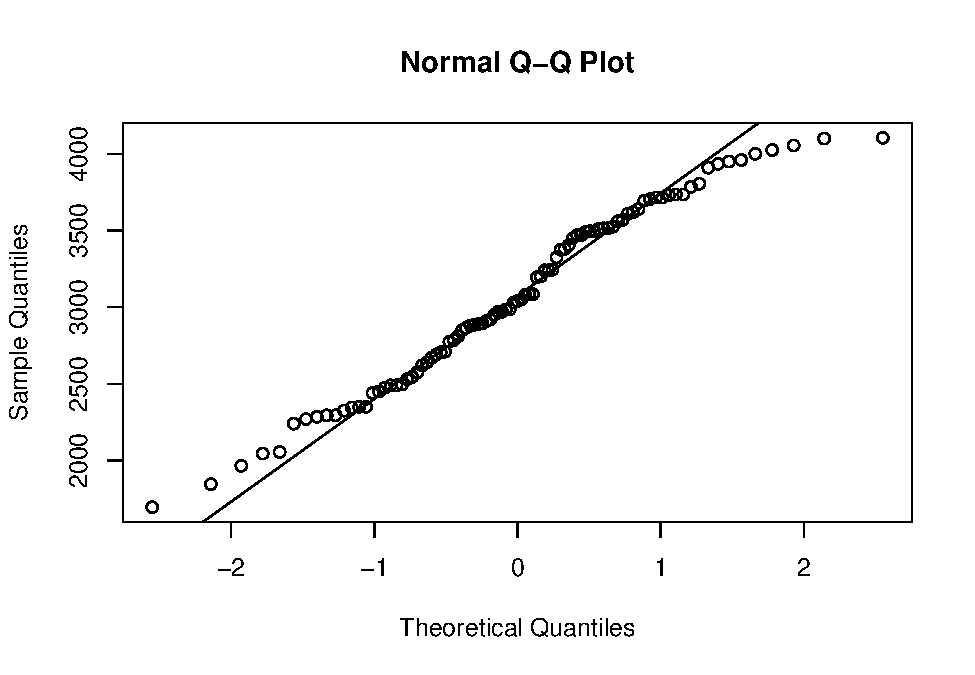
\includegraphics[keepaspectratio]{10-graphics2_files/figure-latex/qq_norm-1.pdf}}

In a similar manner, quantile-quantile plots for other probability distributions can be constructed with the function \texttt{qqplot()}.

\begin{Shaded}
\begin{Highlighting}[]
\NormalTok{y }\OtherTok{\textless{}{-}} \FunctionTok{rexp}\NormalTok{(}\DecValTok{200}\NormalTok{, }\AttributeTok{rate=}\DecValTok{4}\NormalTok{)}
\FunctionTok{qqplot}\NormalTok{ (}\FunctionTok{qexp}\NormalTok{ (}\FunctionTok{seq}\NormalTok{ (}\AttributeTok{from =} \DecValTok{0}\NormalTok{, }\AttributeTok{to =} \DecValTok{1}\NormalTok{, }\AttributeTok{len =} \DecValTok{200}\NormalTok{), }\AttributeTok{rate=}\DecValTok{4}\NormalTok{), y)}
\FunctionTok{qqline}\NormalTok{(y, }\AttributeTok{distribution =} \ControlFlowTok{function}\NormalTok{(p) }\FunctionTok{qexp}\NormalTok{(p, }\AttributeTok{rate=}\DecValTok{4}\NormalTok{))}
\end{Highlighting}
\end{Shaded}

\pandocbounded{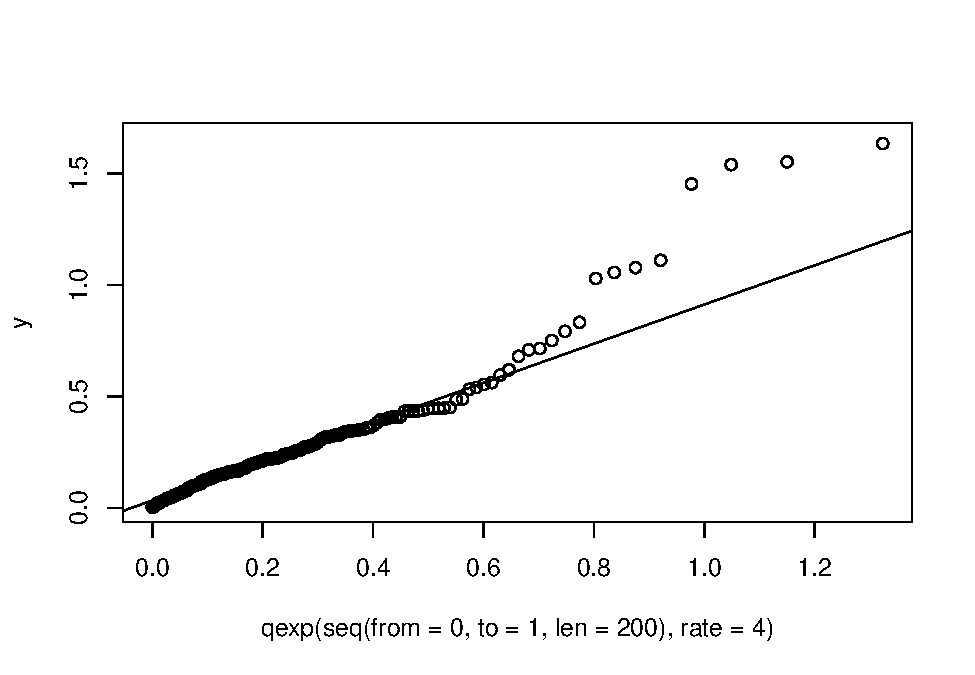
\includegraphics[keepaspectratio]{10-graphics2_files/figure-latex/qq_other-1.pdf}}

\section{Estimating a density}\label{density}

The histograms in Figure \ref{fig:histDiffBins} show 200 observations generated, 100 from a \(normal (9,2^2)\) and 100 from a \(normal (13,1)\) distribution. Histograms are very sensitive to the choice of the number of bins and the starting values of the bins. The wider bins do not show any evidence of a bimodal distribution. Using the smaller bins, the location of the bins can suggest either a bimodal or trimodal distribution.

\begin{figure}
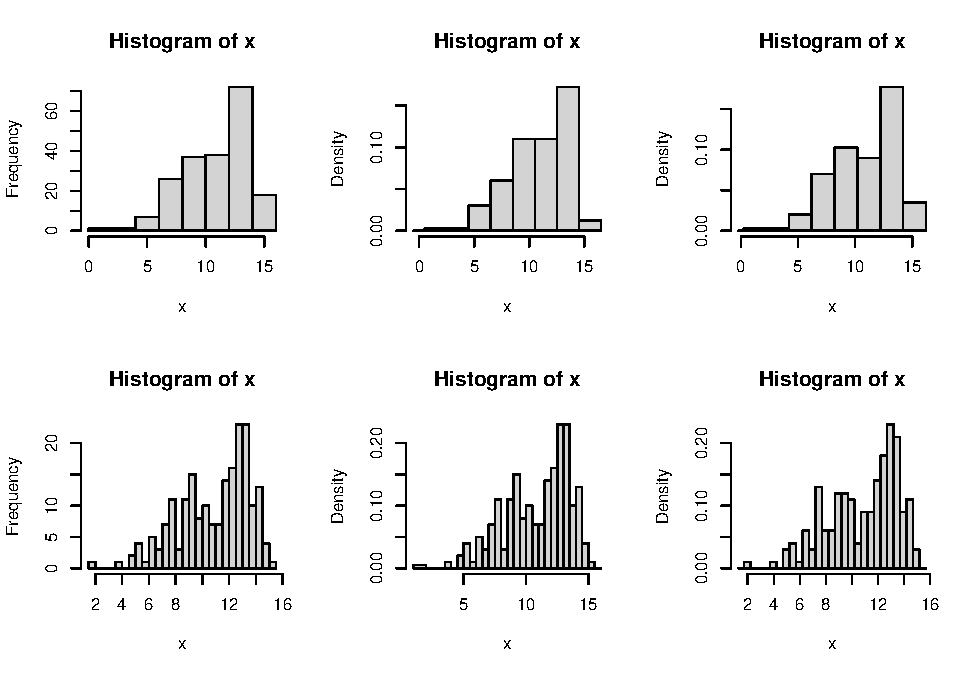
\includegraphics[width=1\linewidth]{10-graphics2_files/figure-latex/histDiffBins-1} \caption{Histograms with different bin sizes and bin locations of the same normal mixture data set.}\label{fig:histDiffBins}
\end{figure}

One possible solution to the bin selection problem for histograms is the Average Shifted Histogram (ASH). First we define a \emph{{density histogram}}. Since we aim to estimate the density (which integrates to one) a density histogram is normalised such that the area in the histogram is equal to one.

Consider a set of bins \(B_k=[b_k, b_{(k+1)})\) with fixed bin width \(λ=b_{(k+1)}-b_k\) \(∀ k\), then the density histogram is defined as \(\hat{f} = \frac{1}{N\lambda} \sum_{i=1}^{N}{I_{[b_k,b_{k+1})}(x_i)}\) for \(x∈B_k\). Consider a collection of \(m\) histograms \(\hat{f}_1, \hat{f}_2, \dots, \hat{f}_m\) each with bin width \(h\), but with respective bin origins \(b_{01}=0, b_{02}=\frac{h}{m}, b_{03}=\frac{2h}{m}, \dots, b_{0m}=\frac{(m-1)h}{m}\). The \emph{{average shifted histogram}} is defined as \(\hat{f}_{ASH} = \frac{1}{m} \sum_{i=1}^{m}{\hat{f}_i}\).

\begin{Shaded}
\begin{Highlighting}[]
\NormalTok{ASH }\OtherTok{\textless{}{-}} \ControlFlowTok{function}\NormalTok{ (x, }\AttributeTok{b0 =} \DecValTok{1}\NormalTok{, }\AttributeTok{bk =} \DecValTok{15}\NormalTok{, }\AttributeTok{h =} \FloatTok{0.5}\NormalTok{, }\AttributeTok{m =} \DecValTok{5}\NormalTok{) }\CommentTok{\# h=lambda}
\NormalTok{\{}
\NormalTok{  Bvec }\OtherTok{\textless{}{-}} \FunctionTok{as.vector}\NormalTok{ ((bk }\SpecialCharTok{{-}}\NormalTok{ b0)}\SpecialCharTok{/}\NormalTok{h}\SpecialCharTok{+}\DecValTok{2}\NormalTok{, }\StringTok{"list"}\NormalTok{)}
\NormalTok{  fhat }\OtherTok{\textless{}{-}} \FunctionTok{matrix}\NormalTok{ (}\AttributeTok{nrow =}\NormalTok{ m, }\AttributeTok{ncol =}\NormalTok{ (bk}\SpecialCharTok{{-}}\NormalTok{b0)}\SpecialCharTok{/}\NormalTok{h}\SpecialCharTok{+}\DecValTok{1}\NormalTok{) }
  \ControlFlowTok{for}\NormalTok{ (i }\ControlFlowTok{in} \DecValTok{1}\SpecialCharTok{:}\NormalTok{m)}
\NormalTok{    \{ Bvec[[i]] }\OtherTok{\textless{}{-}} \FunctionTok{seq}\NormalTok{ (}\AttributeTok{from =}\NormalTok{ b0}\SpecialCharTok{+}\NormalTok{(i}\DecValTok{{-}1}\NormalTok{)}\SpecialCharTok{*}\NormalTok{h}\SpecialCharTok{/}\NormalTok{m, }\AttributeTok{to =}\NormalTok{ bk}\SpecialCharTok{+}\NormalTok{h}\SpecialCharTok{+}\NormalTok{(i}\DecValTok{{-}1}\NormalTok{)}\SpecialCharTok{*}\NormalTok{h}\SpecialCharTok{/}\NormalTok{m, }\AttributeTok{by =}\NormalTok{ h)}
\NormalTok{      fhat[i,] }\OtherTok{\textless{}{-}} \FunctionTok{hist}\NormalTok{ (x, }\AttributeTok{breaks =}\NormalTok{ Bvec[[i]], }\AttributeTok{right =}\NormalTok{ T, }\AttributeTok{plot =}\NormalTok{ F)}\SpecialCharTok{$}\NormalTok{density}
\NormalTok{    \}}
\NormalTok{  fhat.ASH }\OtherTok{\textless{}{-}} \FunctionTok{apply}\NormalTok{(fhat, }\DecValTok{2}\NormalTok{, mean)}
\NormalTok{  x.vec }\OtherTok{\textless{}{-}} \FunctionTok{seq}\NormalTok{ (}\AttributeTok{from =}\NormalTok{ b0, }\AttributeTok{to =}\NormalTok{ bk}\SpecialCharTok{+}\NormalTok{h,}\AttributeTok{length =} \FunctionTok{length}\NormalTok{(fhat.ASH))}
  \FunctionTok{plot}\NormalTok{ (x.vec, fhat.ASH, }\AttributeTok{type=}\StringTok{"l"}\NormalTok{)}
\NormalTok{\}}
\FunctionTok{ASH}\NormalTok{(x, }\AttributeTok{m=}\DecValTok{20}\NormalTok{, }\AttributeTok{h=}\DecValTok{1}\NormalTok{, }\AttributeTok{b0=}\SpecialCharTok{{-}}\DecValTok{2}\NormalTok{, }\AttributeTok{bk=}\DecValTok{18}\NormalTok{)}
\end{Highlighting}
\end{Shaded}

\begin{figure}
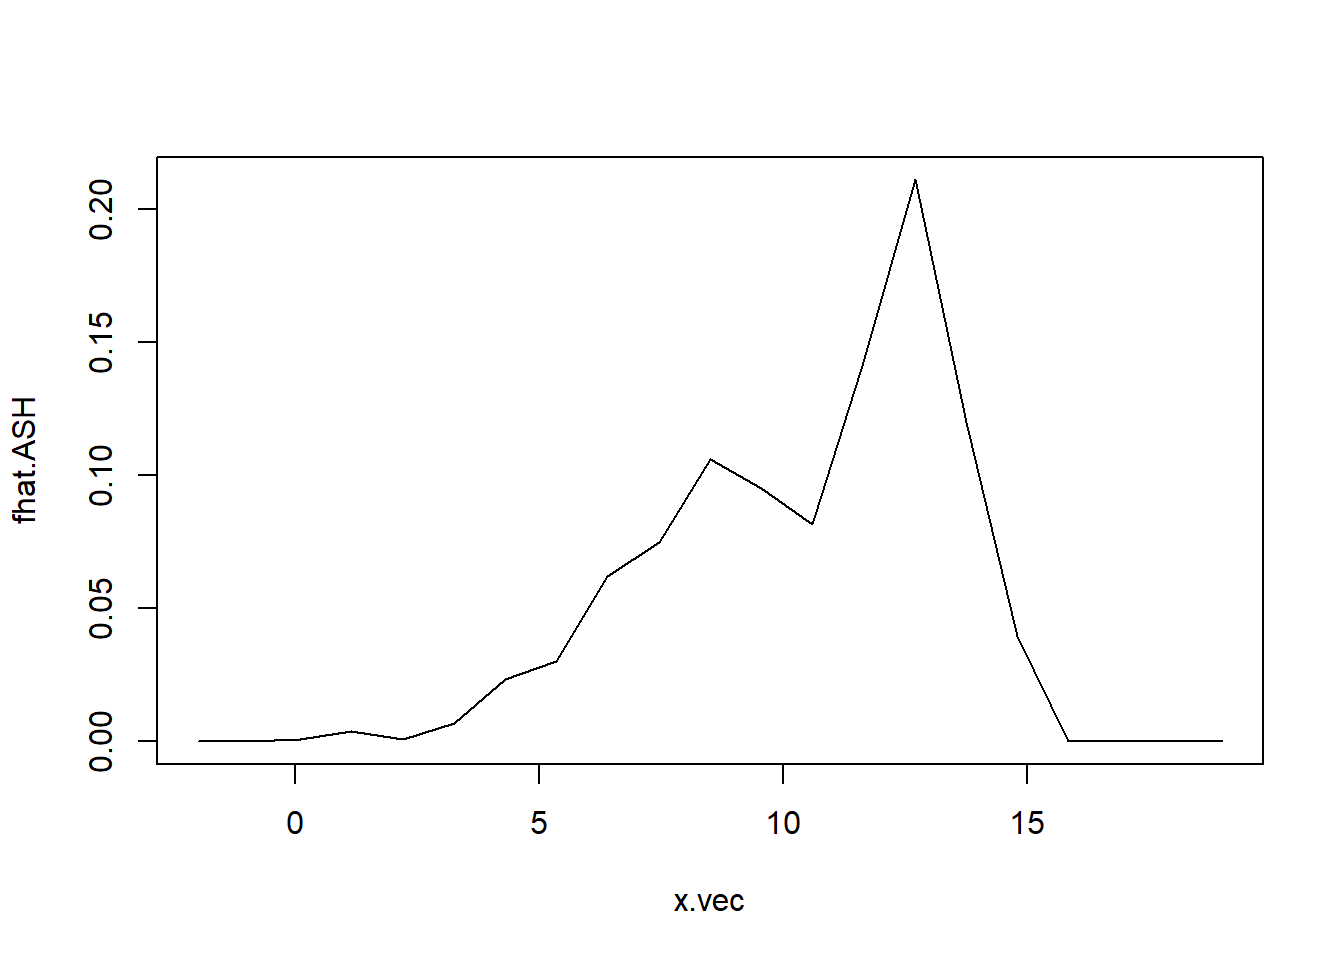
\includegraphics[width=1\linewidth]{10-graphics2_files/figure-latex/ASH-1} \caption{Average shifted histogram of normal mixture data.}\label{fig:ASH}
\end{figure}

The ASH is given in Figure \ref{fig:ASH} A more sophisticated method for estimating a density is with a kernel density estimate. The density histograms is replaced by a smooth kernel function, leading to a smoother estimate. The R function \texttt{density()} provides a variety of kernels. Using the default kernel, a Gaussian distribution, the kernel density estimate is given in Figure \ref{fig:densityExample}.

\begin{Shaded}
\begin{Highlighting}[]
\FunctionTok{plot}\NormalTok{(}\FunctionTok{density}\NormalTok{(x), }\AttributeTok{type=}\StringTok{"l"}\NormalTok{)}
\end{Highlighting}
\end{Shaded}

\begin{figure}
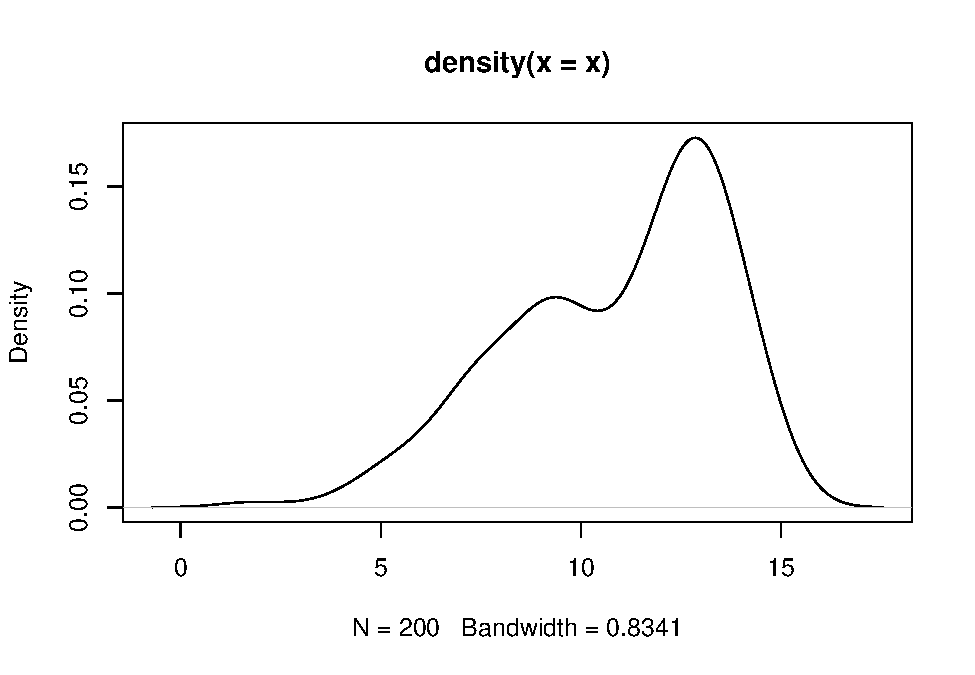
\includegraphics[width=1\linewidth]{10-graphics2_files/figure-latex/densityExample-1} \caption{Guassian kernel density estimate of the normal mixture data.}\label{fig:densityExample}
\end{figure}

Experiment with different kernel function and different choices of bandwidth (argument bw) for controlling the amount of smoothing.

\section{A coplot with two conditioning variables}\label{coplot}

Consider the \texttt{state.x77} data set. In section \ref{highLevelPlotting} the \texttt{coplot()} function was used to construct a plot of \texttt{Illiteracy} and \texttt{Area} conditional on \texttt{Income}. This can be expanded to two conditions, for example plotting \texttt{Illiteracy} and \texttt{Life\ expectancy} conditional on \texttt{Income} and \texttt{Area}. Interpret. The number of panels and overlap of given intervals can be controlled with the arguments number and overlap.

\begin{Shaded}
\begin{Highlighting}[]
\FunctionTok{coplot}\NormalTok{ (state.x77 [,}\StringTok{"Illiteracy"}\NormalTok{] }\SpecialCharTok{\textasciitilde{}}\NormalTok{ state.x77 [,}\StringTok{"Life Exp"}\NormalTok{] }\SpecialCharTok{|} 
\NormalTok{                                   state.x77 [,}\StringTok{"Income"}\NormalTok{] }\SpecialCharTok{+}\NormalTok{ state.x77 [,}\StringTok{"Area"}\NormalTok{], }
                                \AttributeTok{number =} \FunctionTok{c}\NormalTok{(}\DecValTok{4}\NormalTok{,}\DecValTok{3}\NormalTok{), }\AttributeTok{overlap=}\FunctionTok{c}\NormalTok{(}\DecValTok{0}\NormalTok{,}\FloatTok{0.2}\NormalTok{))}
\end{Highlighting}
\end{Shaded}

\pandocbounded{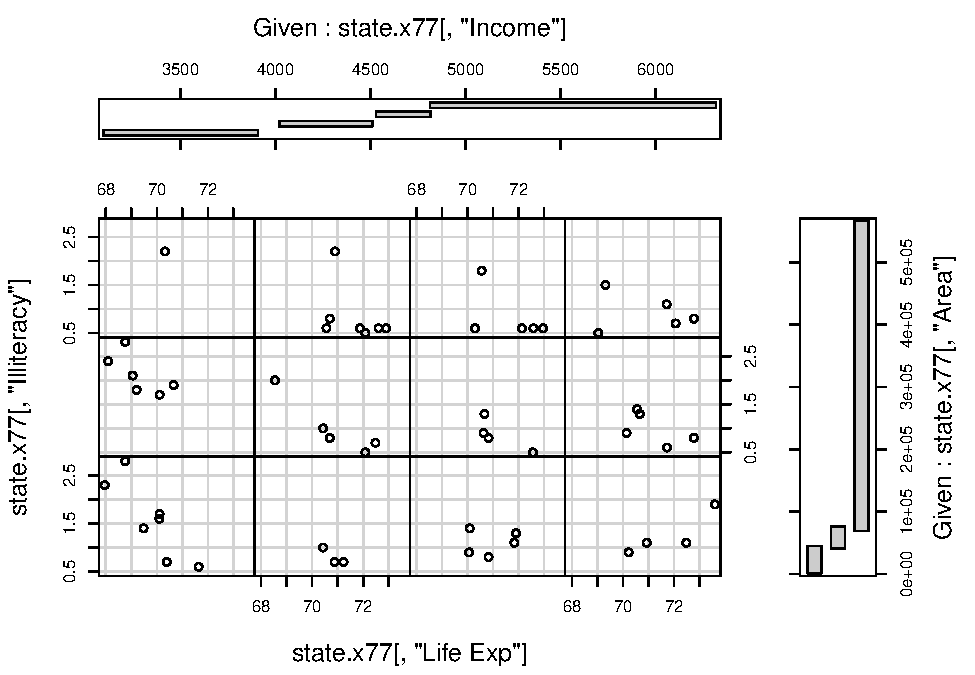
\includegraphics[keepaspectratio]{10-graphics2_files/figure-latex/condIncomeArea-1.pdf}}

\section{Exact distances in graphics}\label{exact-distances-in-graphics}

\begin{enumerate}
\def\labelenumi{(\alph{enumi})}
\tightlist
\item
  Obtain a random sample of size 50 from a bivariate normal distribution with \(n(50,20)\) marginals and a correlation coefficient of 0.90.
\end{enumerate}

\begin{itemize}
\item
  Present the data in the form of a scatterplot.
\item
  Next, write an R function to perform the following task on the scatterplot:

  \begin{itemize}
  \item
    Choose an arbitrary point and label it ``A''.
  \item
    Draw a line connecting A to a circle with centre exactly 25mm away from A. The diameter of the circle must be exactly 40mm.
  \item
    Label the centre point of the circle with a ``B''.
  \item
    Use a ruler to check the length of the connecting line and diameter of the circle.
  \end{itemize}
\item
  Obtain a print copy of the graph and check the lengths again.\emph{Hint}: Study the help file of function \texttt{par()}.
\end{itemize}

\begin{enumerate}
\def\labelenumi{(\alph{enumi})}
\setcounter{enumi}{1}
\tightlist
\item
  Use R to make a ruler calibrated in centimetres from zero to 15 cms.
\end{enumerate}

\section{Multiple graphics windows in R}\label{multiple-graphics-windows-in-r}

\begin{enumerate}
\def\labelenumi{(\alph{enumi})}
\tightlist
\item
  Study how the following instructions work to control multiple graphics windows in R:
\end{enumerate}

\begin{Shaded}
\begin{Highlighting}[]
\FunctionTok{dev.new}\NormalTok{() }
\FunctionTok{dev.list}\NormalTok{()  }
\FunctionTok{dev.set}\NormalTok{()   }
\FunctionTok{dev.next}\NormalTok{()}
\FunctionTok{dev.cur}\NormalTok{()   }
\FunctionTok{dev.copy}\NormalTok{()  }
\FunctionTok{dev.prev}\NormalTok{()}
\FunctionTok{dev.off}\NormalTok{()   }
\FunctionTok{dev.ask}\NormalTok{()   }
\FunctionTok{graphics.off}\NormalTok{()}
\end{Highlighting}
\end{Shaded}

\begin{enumerate}
\def\labelenumi{(\alph{enumi})}
\setcounter{enumi}{1}
\tightlist
\item
  Study the information that R gives via the execution of \texttt{help.search\ ("graph")}.
\end{enumerate}

\section{More complex layouts}\label{more-complex-layouts}

Study the graphical requirements needed for constructing Figure \ref{fig:complexLayout} and how to code these requirements.

\begin{Shaded}
\begin{Highlighting}[]
\NormalTok{my.func }\OtherTok{\textless{}{-}} \ControlFlowTok{function}\NormalTok{ () }
\NormalTok{\{ old.state }\OtherTok{\textless{}{-}} \FunctionTok{par}\NormalTok{ (}\AttributeTok{no.readonly =} \ConstantTok{TRUE}\NormalTok{)}
 \FunctionTok{on.exit}\NormalTok{ (}\FunctionTok{par}\NormalTok{ (old.state))}
   
 \FunctionTok{par}\NormalTok{ (}\AttributeTok{omd =} \FunctionTok{c}\NormalTok{(}\DecValTok{0}\NormalTok{, }\FloatTok{0.66}\NormalTok{, }\DecValTok{0}\NormalTok{, }\DecValTok{1}\NormalTok{), }\AttributeTok{mfcol =} \FunctionTok{c}\NormalTok{(}\DecValTok{2}\NormalTok{, }\DecValTok{1}\NormalTok{))}
 \FunctionTok{ts.plot}\NormalTok{ (mdeaths, }\AttributeTok{xlab =} \StringTok{"Year"}\NormalTok{, }\AttributeTok{ylab =} \StringTok{"Male deaths"}\NormalTok{)}
 \FunctionTok{ts.plot}\NormalTok{ (fdeaths, }\AttributeTok{xlab =} \StringTok{"Year"}\NormalTok{, }\AttributeTok{ylab =} \StringTok{"Female deaths"}\NormalTok{)}

 \FunctionTok{par}\NormalTok{ (}\AttributeTok{omd =} \FunctionTok{c}\NormalTok{(}\FloatTok{0.66}\NormalTok{, }\DecValTok{1}\NormalTok{, }\DecValTok{0}\NormalTok{, }\DecValTok{1}\NormalTok{), }\AttributeTok{mfcol =} \FunctionTok{c}\NormalTok{(}\DecValTok{2}\NormalTok{, }\DecValTok{1}\NormalTok{), }\AttributeTok{mfg =} \FunctionTok{c}\NormalTok{(}\DecValTok{1}\NormalTok{, }\DecValTok{1}\NormalTok{), }\AttributeTok{new=}\ConstantTok{TRUE}\NormalTok{)}
 \FunctionTok{hist}\NormalTok{ (mdeaths, }\AttributeTok{xlab =} \StringTok{"Male deaths"}\NormalTok{, }\AttributeTok{ylab =} \StringTok{"Frequency"}\NormalTok{, }\AttributeTok{main =} \StringTok{""}\NormalTok{)}
 \FunctionTok{hist}\NormalTok{ (fdeaths, }\AttributeTok{xlab =} \StringTok{"Female deaths"}\NormalTok{, }\AttributeTok{ylab =} \StringTok{"Frequency"}\NormalTok{, }\AttributeTok{main=} \StringTok{""}\NormalTok{)}

 \FunctionTok{par}\NormalTok{ (}\AttributeTok{omd =} \FunctionTok{c}\NormalTok{(}\DecValTok{0}\NormalTok{, }\DecValTok{1}\NormalTok{, }\DecValTok{0}\NormalTok{, }\DecValTok{1}\NormalTok{), }\AttributeTok{mfcol =} \FunctionTok{c}\NormalTok{(}\DecValTok{1}\NormalTok{, }\DecValTok{1}\NormalTok{))}
 \FunctionTok{title}\NormalTok{ (}\StringTok{"Line plot and Histogram for male deaths"}\NormalTok{)}
   
 \FunctionTok{par}\NormalTok{(}\AttributeTok{omd =} \FunctionTok{c}\NormalTok{(}\DecValTok{0}\NormalTok{, }\DecValTok{1}\NormalTok{, }\DecValTok{0}\NormalTok{, }\FloatTok{0.5}\NormalTok{), }\AttributeTok{mfcol =} \FunctionTok{c}\NormalTok{(}\DecValTok{1}\NormalTok{, }\DecValTok{1}\NormalTok{))}
 \FunctionTok{title}\NormalTok{ (}\StringTok{"Line plot and Histogram for female deaths"}\NormalTok{)          }
\NormalTok{\}}
\FunctionTok{my.func}\NormalTok{ ()}
\end{Highlighting}
\end{Shaded}

\begin{figure}
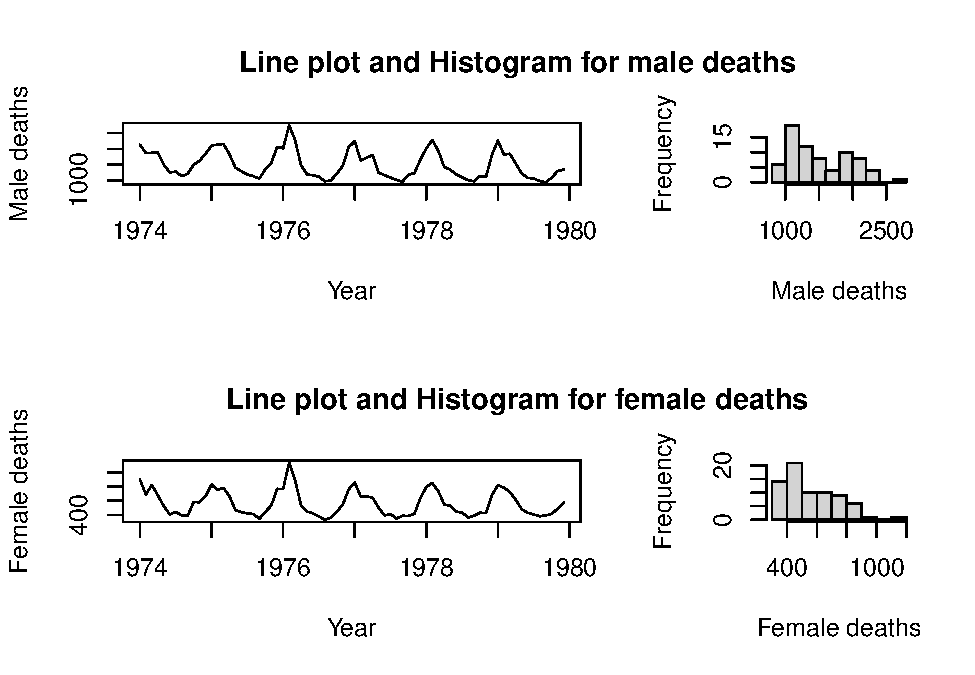
\includegraphics[width=1\linewidth]{10-graphics2_files/figure-latex/complexLayout-1} \caption{A complex graphics layout.}\label{fig:complexLayout}
\end{figure}

\section{Dynamic 3D graphics in R}\label{dynamic-3d-graphics-in-r}

\begin{itemize}
\item
  Study the R package \texttt{rgl}.
\item
  Attach library \texttt{rgl} to the search path and then issue the R command \texttt{example\ (plot3d)}. Use the mouse buttons to rotate and zoom the rgl graph.
\item
  Next, issue the R command \texttt{example\ (surface3d)} and interactively explore the 3D figure.
\end{itemize}

\section{Animation}\label{animation}

Study the following two functions in detail:

\begin{Shaded}
\begin{Highlighting}[]
\NormalTok{anim1 }\OtherTok{\textless{}{-}} \ControlFlowTok{function}\NormalTok{ (}\AttributeTok{sleep =} \FloatTok{0.05}\NormalTok{) }
\NormalTok{ \{ }\CommentTok{\# Press ESC to end animation}
\NormalTok{   n }\OtherTok{\textless{}{-}} \DecValTok{40}
\NormalTok{   t }\OtherTok{\textless{}{-}} \FunctionTok{seq}\NormalTok{ (}\DecValTok{0}\NormalTok{, }\DecValTok{2}\SpecialCharTok{*}\NormalTok{pi, }\AttributeTok{length =}\NormalTok{ n)}
\NormalTok{   x }\OtherTok{\textless{}{-}} \FunctionTok{cos}\NormalTok{(t)}
\NormalTok{   y }\OtherTok{\textless{}{-}} \FunctionTok{sin}\NormalTok{(t)}
   \ControlFlowTok{for}\NormalTok{ (i }\ControlFlowTok{in} \DecValTok{1}\SpecialCharTok{:}\NormalTok{n)}
\NormalTok{   \{  }\FunctionTok{plot.new}\NormalTok{ ()}
      \FunctionTok{plot.window}\NormalTok{ (}\FunctionTok{c}\NormalTok{(}\SpecialCharTok{{-}}\DecValTok{1}\NormalTok{, }\DecValTok{1}\NormalTok{), }\FunctionTok{c}\NormalTok{(}\SpecialCharTok{{-}}\DecValTok{1}\NormalTok{, }\DecValTok{1}\NormalTok{), }\AttributeTok{asp =} \DecValTok{1}\NormalTok{)}
      \FunctionTok{points}\NormalTok{ (x[i], y[i], }\AttributeTok{pch =} \DecValTok{16}\NormalTok{, }\AttributeTok{cex =} \DecValTok{2}\NormalTok{)}
      \FunctionTok{Sys.sleep}\NormalTok{(sleep) }
      \CommentTok{\#Sys.sleep() suspends execution for a given number of seconds}
\NormalTok{    \}}
   \FunctionTok{Recall}\NormalTok{(sleep) }
\NormalTok{ \}}

\NormalTok{anim2 }\OtherTok{\textless{}{-}} \ControlFlowTok{function}\NormalTok{ (}\AttributeTok{sleep =} \FloatTok{0.01}\NormalTok{) }
\NormalTok{\{ }\ControlFlowTok{for}\NormalTok{ (i }\ControlFlowTok{in} \FunctionTok{seq}\NormalTok{ (}\AttributeTok{from =} \DecValTok{1}\NormalTok{, }\AttributeTok{to =} \DecValTok{3}\NormalTok{, }\AttributeTok{by =} \FloatTok{0.01}\NormalTok{))}
\NormalTok{  \{  }\FunctionTok{plot.new}\NormalTok{ ()}
     \FunctionTok{plot.window}\NormalTok{ (}\FunctionTok{c}\NormalTok{ (}\DecValTok{1}\NormalTok{, }\DecValTok{16}\NormalTok{), }\FunctionTok{c}\NormalTok{(}\DecValTok{1}\NormalTok{, }\DecValTok{16}\NormalTok{), }\AttributeTok{asp =} \DecValTok{1}\NormalTok{)}
     \FunctionTok{arrows}\NormalTok{(}\DecValTok{2}\SpecialCharTok{*}\NormalTok{i, }\DecValTok{2}\SpecialCharTok{*}\NormalTok{i, }\DecValTok{4}\SpecialCharTok{*}\NormalTok{i, }\DecValTok{4}\SpecialCharTok{*}\NormalTok{i)}
     \FunctionTok{Sys.sleep}\NormalTok{(sleep)}
\NormalTok{  \}}
  \FunctionTok{Recall}\NormalTok{(sleep)}
\NormalTok{\}}
\end{Highlighting}
\end{Shaded}

Write an R function to show a wheel with two spokes moving forward with adjustable speed.

\section{Exercise}\label{Ex10}

\begin{enumerate}
\def\labelenumi{(\arabic{enumi})}
\tightlist
\item
  In many real life situations it is necessary to identify an object when only limited information is available. The following problem how such a problem can be empirically investigated.
\end{enumerate}

The function \texttt{persp()} used for constructing Figure \ref{fig:persp} requires a regular pattern of \(x\) and \(y\) coordinates. If such a pattern is not available it is necessary to interpolate e.g.~with \texttt{interp()} (available in package \texttt{akima}) using the available values.

Use the function \texttt{expand.grid()} to create a grid of regularly spaced \(x\) and \(y\) values and evaluate the ``sombrero'' function of Figure \ref{fig:persp} at each of these points.

Now use \texttt{sample()} to randomly sample points from that grid and then the \texttt{interp()} function to interpolate the values of z throughout the grid.

Finally, use \texttt{persp()} to construct a plot of the interpolated values.

What fraction of data is needed in the sample to get a good representation of the true shape of the data. \emph{Hint}: since \texttt{persp()} does not accept \texttt{NA}s replace \texttt{NA}s with the minimum of the non-missing z values.

\begin{enumerate}
\def\labelenumi{(\arabic{enumi})}
\setcounter{enumi}{1}
\item
  Use \texttt{locator()} and write a function to allow placing a legend with a pointing device anywhere on an existing plot.
\item
  Use the \texttt{state.x77} data set to construct a scatterplot of \texttt{Illiteracy} as a function of \texttt{Income}. Now construct a second scatterplot of the same data but with the origin on the right-hand side of the x-axis. In order to complete this task it is necessary that the values on the x-axis increase from the left-hand side to the right-hand side.
\item
  Consider the following data
\end{enumerate}

\begin{longtable}[]{@{}lllll@{}}
\toprule\noalign{}
& Test 1 & Test 2 & Test 3 & Test 4 \\
\midrule\noalign{}
\endhead
\bottomrule\noalign{}
\endlastfoot
Group A: & 10 & 15 & 30 & 12 \\
Group B: & 125 & 130 & 148 & 115 \\
\end{longtable}

Plot the data of the two groups in the form of two profiles on the same set of axes.\\
Plot the data against Test 1, Test 2, Test 3 and Test 4 on the x-axis.
The scale of the data of Group A must appear on the y-axis on the left-hand side and that of Group B on the y-axis on the right-hand side. A detailed legend must be provided.

\section{The package ggplot2}\label{the-package-ggplot2}

The package \texttt{ggplot2} is based on the ideas of \citet{Wickham2010} as described in the paper ``A layered grammar of graphics'' and makes use of the The Grammar of Graphics by \citet{Wilkenson2005}.

\begin{figure}
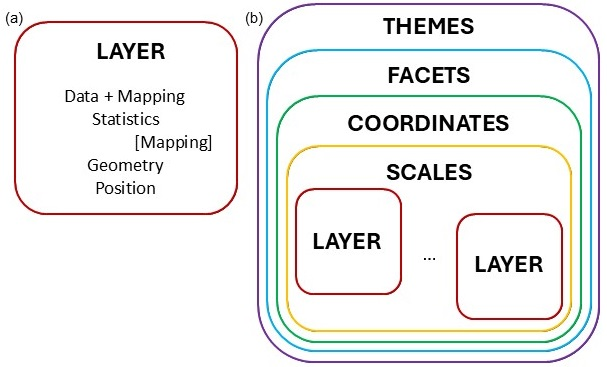
\includegraphics[width=1\linewidth]{pics/ggplot} \caption{Layer structure of ggplot2 package.}\label{fig:ggplotStructure}
\end{figure}

In Figure \ref{fig:ggplotStructure}(a) the components of a \emph{{layer}} is depicted. The first essential component is the \emph{{data}} to be represented in the graphic. Together with the data, there needs to be an \emph{{aesthetic mapping}}, describing which variable is mapped to the x-direction, y-direction, the size, shape, colour, etc. The \emph{{statistics}} component optionally transforms the data to quantities that needs to be plotted. Typically, the transformation is used to summarise the data. It is possible to map aesthetics to these new variables. The \emph{{geometry}} defines how each aesthetic is displayed, as points, lines, boxplots, densities, histograms, etc. Each geometry can only display specific aesthetics, for example a point has position, colour, shape and size. Position adjustment is needed in cases where geometric elements overlap, for example using jitter in scatterplots or placing multiple bars stacked or side-by-side in a barplot.

A graphic can consist of several layers, as shown in Figure \ref{fig:ggplotStructure}(b). According to the grammar of graphics, a \emph{{scales}} component needs to be specified. The scales are common across layers and describe the mapping of the data to aesthetic attributes such as which colour is associated with which level of a categorical variable. One scale is needed for each aesthetic property used in the layers. In order to place the geometric objects on the plotting plane, a scale is needed. The most commonly used scale is the Cartesian axes, while others such as polar coordinates is also available.

\emph{{Faceting}} splits the data into small multiples of different subsets of the data set. With this component we identify the variable(s) for splitting and how the splitting should be arranged. \emph{{Themes}} are not linked to the data but provide instructions on aspects such as titles, labels, fonts, background, gridlines, and legends.

The full specification of all the components in a ggplot, can be very cumbersome. Defaults are specified, for instance for each geometry there is a default statistic and for each statistic a default geometry. We can therefore build our plot stepwise, fine-tuning detailed aspects until the required graphic is obtained.

We will start with some simple plots and then build more complicated graphics. We will use the \texttt{cereal} tibble created from the \texttt{UScereal} data in package \texttt{MASS} (see section \ref{dplyr}) for illustration.

\begin{Shaded}
\begin{Highlighting}[]
\FunctionTok{library}\NormalTok{ (MASS)}
\FunctionTok{library}\NormalTok{ (tidyverse)}
\CommentTok{\#\textgreater{} {-}{-} Attaching core tidyverse packages {-}{-}{-}{-} tidyverse 2.0.0 {-}{-}}
\CommentTok{\#\textgreater{} v dplyr     1.1.4     v readr     2.1.5}
\CommentTok{\#\textgreater{} v forcats   1.0.0     v stringr   1.5.1}
\CommentTok{\#\textgreater{} v ggplot2   3.5.2     v tibble    3.3.0}
\CommentTok{\#\textgreater{} v lubridate 1.9.4     v tidyr     1.3.1}
\CommentTok{\#\textgreater{} v purrr     1.1.0     }
\CommentTok{\#\textgreater{} {-}{-} Conflicts {-}{-}{-}{-}{-}{-}{-}{-}{-}{-}{-}{-}{-}{-}{-}{-}{-}{-}{-}{-}{-}{-} tidyverse\_conflicts() {-}{-}}
\CommentTok{\#\textgreater{} x dplyr::filter() masks stats::filter()}
\CommentTok{\#\textgreater{} x dplyr::lag()    masks stats::lag()}
\CommentTok{\#\textgreater{} x dplyr::select() masks MASS::select()}
\CommentTok{\#\textgreater{} i Use the conflicted package (\textless{}http://conflicted.r{-}lib.org/\textgreater{}) to force all conflicts to become errors}
\NormalTok{cereal }\OtherTok{\textless{}{-}} \FunctionTok{tibble}\NormalTok{ (UScereal)}
\end{Highlighting}
\end{Shaded}

\subsection{Barplot}\label{barplot}

The command

\begin{Shaded}
\begin{Highlighting}[]
\FunctionTok{ggplot}\NormalTok{(}\AttributeTok{data =}\NormalTok{ cereal, }
       \AttributeTok{mapping =} \FunctionTok{aes}\NormalTok{(}\AttributeTok{x =}\NormalTok{ mfr)) }\SpecialCharTok{+}   
       \FunctionTok{geom\_bar}\NormalTok{()}
\end{Highlighting}
\end{Shaded}

\pandocbounded{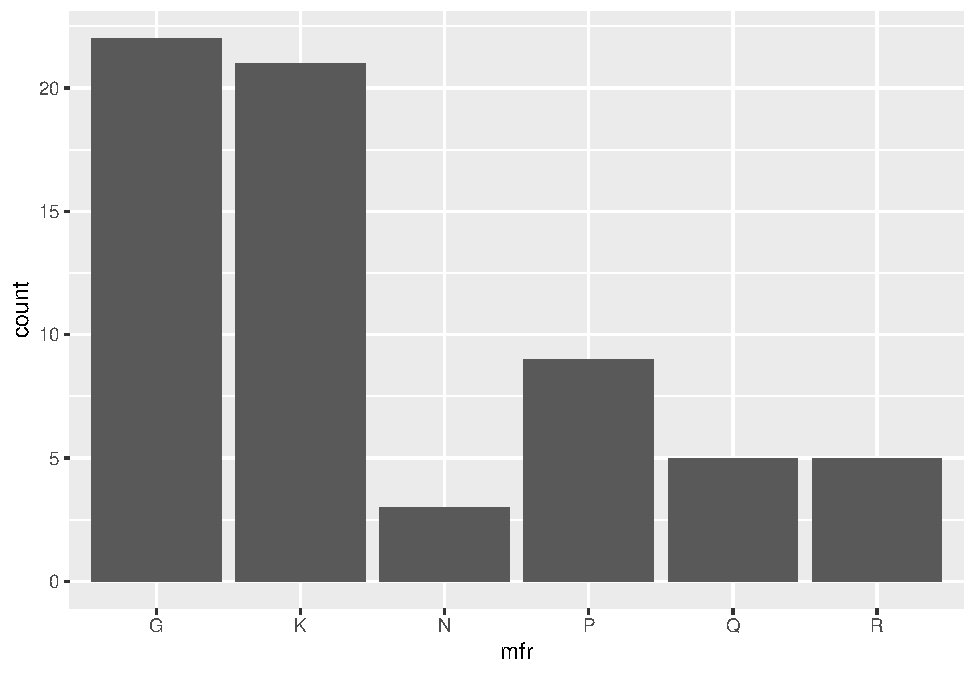
\includegraphics[keepaspectratio]{10-graphics2_files/figure-latex/ggplotBarplot-1.pdf}}

produces a simple barplot of the \texttt{cereal} data with \texttt{mfr} on the x-axis and counts of each level in the \texttt{bars}. No position adjustments are made, while the default colour for the bars is used to plot the complete data set on Cartesian axes with the default theme.

We can change the colour of the bars with the command

\begin{Shaded}
\begin{Highlighting}[]
\FunctionTok{ggplot}\NormalTok{(}\AttributeTok{data =}\NormalTok{ cereal, }
       \AttributeTok{mapping =} \FunctionTok{aes}\NormalTok{(}\AttributeTok{x =}\NormalTok{ mfr)) }\SpecialCharTok{+}   
       \FunctionTok{geom\_bar}\NormalTok{(}\AttributeTok{fill =} \StringTok{"gold"}\NormalTok{)}
\end{Highlighting}
\end{Shaded}

\pandocbounded{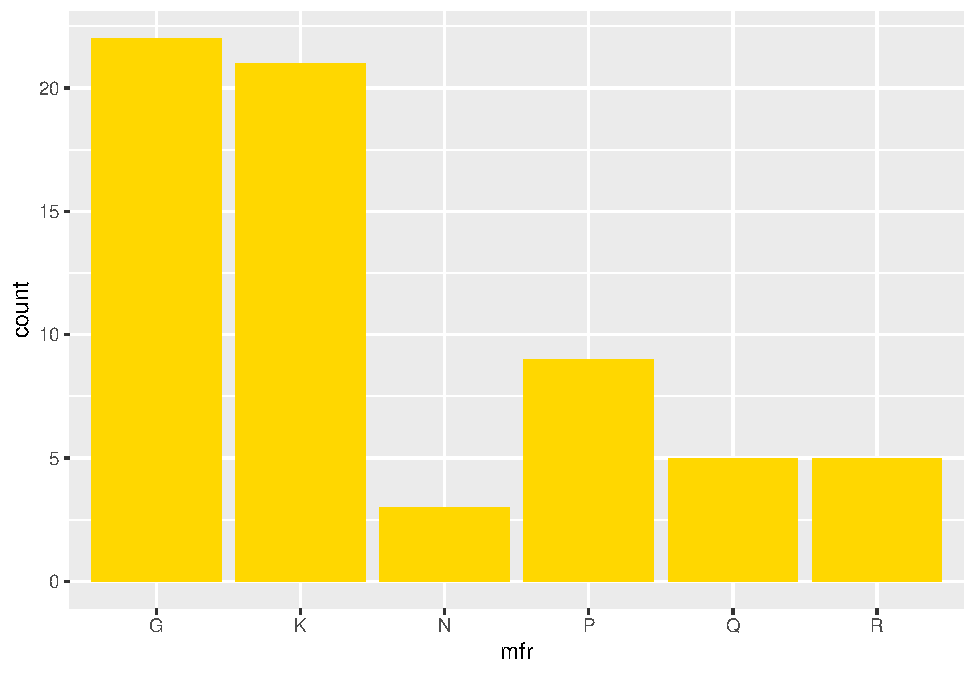
\includegraphics[keepaspectratio]{10-graphics2_files/figure-latex/ggplotBarplot2-1.pdf}}

Now we add an aesthetic for the bars to be coloured according to the vitamin enrichment, while at the same time, changing the orientation. Note that in the previous example, the fill colour was specified outside of the function \texttt{aes()}, while here, it is specified as an aesthetic.

\begin{Shaded}
\begin{Highlighting}[]
\FunctionTok{ggplot}\NormalTok{(}\AttributeTok{data =}\NormalTok{ cereal, }
       \AttributeTok{mapping =} \FunctionTok{aes}\NormalTok{(}\AttributeTok{y =}\NormalTok{ mfr, }\AttributeTok{fill =}\NormalTok{ vitamins)) }\SpecialCharTok{+}   
       \FunctionTok{geom\_bar}\NormalTok{() }
\end{Highlighting}
\end{Shaded}

\pandocbounded{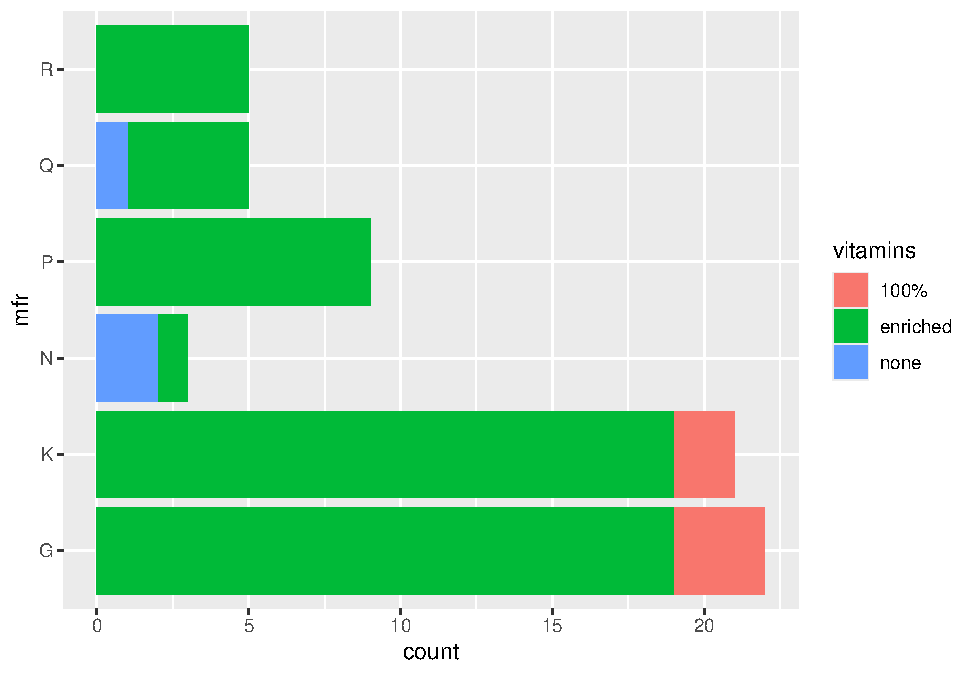
\includegraphics[keepaspectratio]{10-graphics2_files/figure-latex/ggplotBarplot3-1.pdf}}

The default is to stack the bars. In order to position the bars side-by-side we use the function \texttt{position\_dodge()}.

\begin{Shaded}
\begin{Highlighting}[]
\FunctionTok{ggplot}\NormalTok{(}\AttributeTok{data =}\NormalTok{ cereal, }
       \AttributeTok{mapping =} \FunctionTok{aes}\NormalTok{(}\AttributeTok{y =}\NormalTok{ mfr, }\AttributeTok{fill =}\NormalTok{ vitamins)) }\SpecialCharTok{+}   
       \FunctionTok{geom\_bar}\NormalTok{(}\AttributeTok{position =} \FunctionTok{position\_dodge}\NormalTok{())}
\end{Highlighting}
\end{Shaded}

\pandocbounded{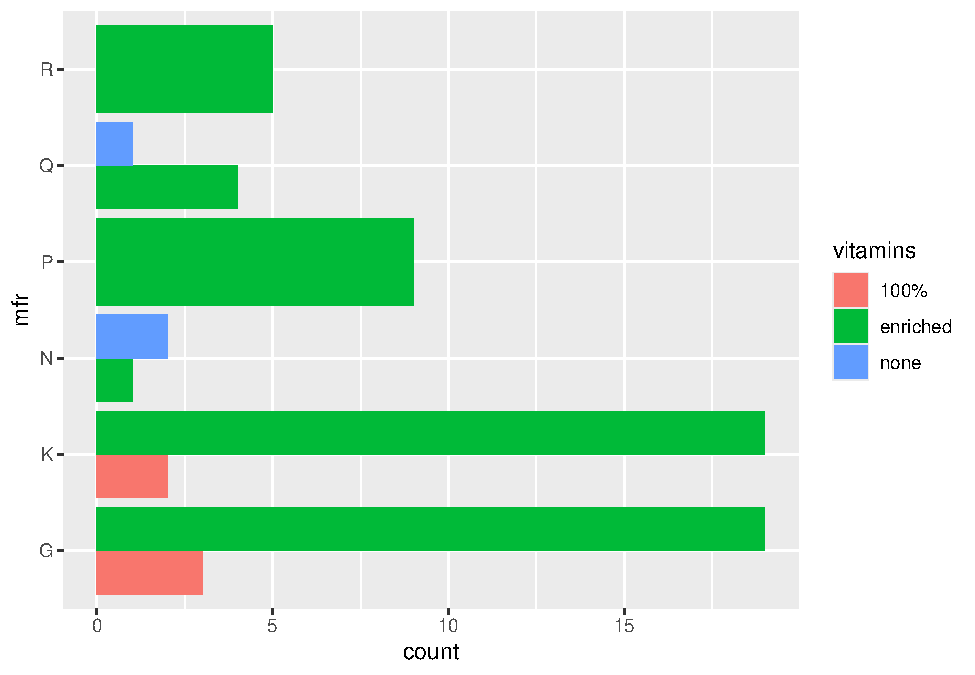
\includegraphics[keepaspectratio]{10-graphics2_files/figure-latex/ggplotBatplot4-1.pdf}}

\subsection{Scatterplot}\label{scatterplot}

The simplest call to produce a scatterplot uses the identity statistical transformation with no position adjustment on the complete data set with default size, shape and colour of the plotting characters.

\begin{Shaded}
\begin{Highlighting}[]
\FunctionTok{ggplot}\NormalTok{(}\AttributeTok{data =}\NormalTok{ cereal, }
       \AttributeTok{mapping =} \FunctionTok{aes}\NormalTok{(}\AttributeTok{x =}\NormalTok{ calories, }\AttributeTok{y =}\NormalTok{ fat)) }\SpecialCharTok{+}        
       \FunctionTok{geom\_point}\NormalTok{()}
\end{Highlighting}
\end{Shaded}

\pandocbounded{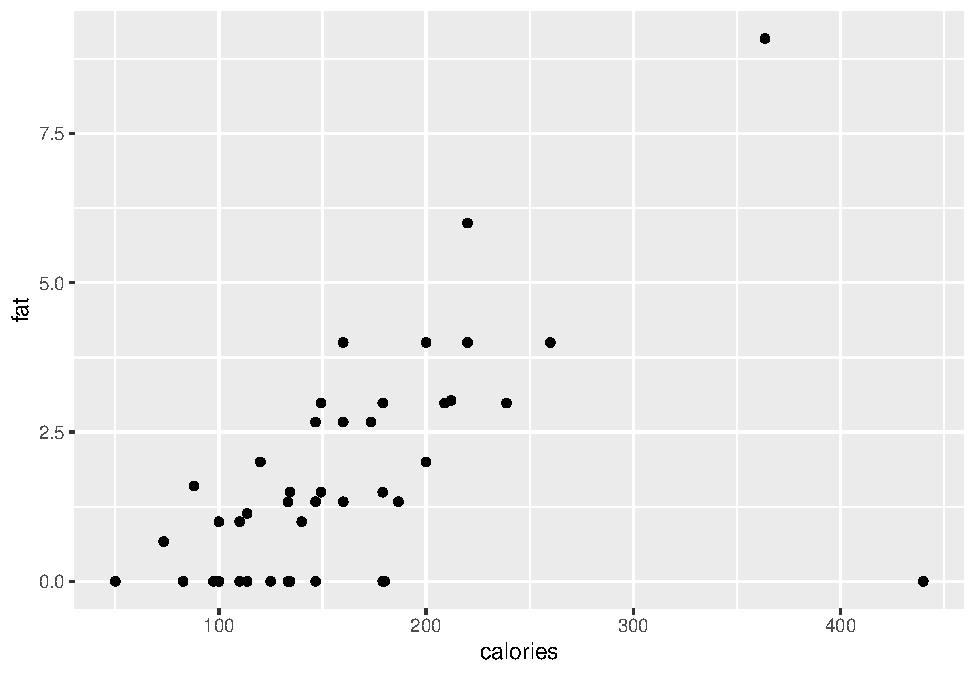
\includegraphics[keepaspectratio]{10-graphics2_files/figure-latex/ggplotScatter-1.pdf}}

The point colours can be specified either according to a categorical variable, or a spectra based on a continuous variable.

\begin{Shaded}
\begin{Highlighting}[]
\FunctionTok{ggplot}\NormalTok{(}\AttributeTok{data =}\NormalTok{ cereal, }
       \AttributeTok{mapping =} \FunctionTok{aes}\NormalTok{(}\AttributeTok{x =}\NormalTok{ calories, }\AttributeTok{y =}\NormalTok{ fat)) }\SpecialCharTok{+} 
       \FunctionTok{geom\_point}\NormalTok{(}\AttributeTok{mapping =} \FunctionTok{aes}\NormalTok{(}\AttributeTok{colour =} \FunctionTok{factor}\NormalTok{(shelf)))}
\end{Highlighting}
\end{Shaded}

\pandocbounded{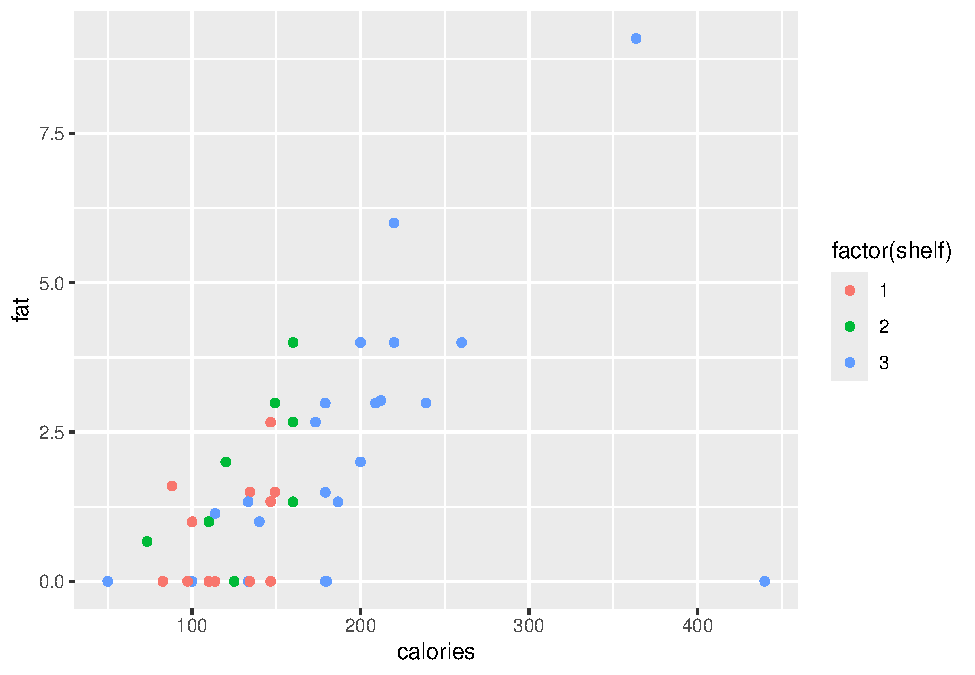
\includegraphics[keepaspectratio]{10-graphics2_files/figure-latex/ggplotScatter2-1.pdf}}

\begin{Shaded}
\begin{Highlighting}[]

\FunctionTok{ggplot}\NormalTok{(}\AttributeTok{data =}\NormalTok{ cereal, }
       \AttributeTok{mapping =} \FunctionTok{aes}\NormalTok{(}\AttributeTok{x =}\NormalTok{ calories, }\AttributeTok{y =}\NormalTok{ fat)) }\SpecialCharTok{+} 
       \FunctionTok{geom\_point}\NormalTok{(}\AttributeTok{mapping =} \FunctionTok{aes}\NormalTok{(}\AttributeTok{colour =}\NormalTok{ sugars))}
\end{Highlighting}
\end{Shaded}

\pandocbounded{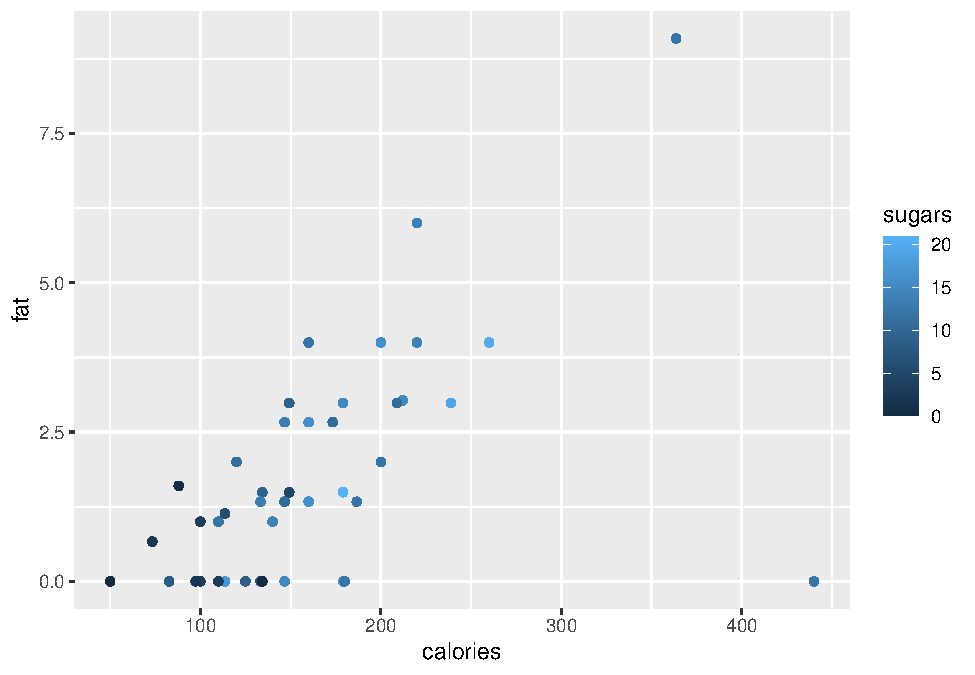
\includegraphics[keepaspectratio]{10-graphics2_files/figure-latex/ggplotScatter2-2.pdf}}

A scatterplot smoother can be added to our plot with the function \texttt{geom\_smooth()}.

\begin{Shaded}
\begin{Highlighting}[]
\FunctionTok{ggplot}\NormalTok{(}\AttributeTok{data =}\NormalTok{ cereal, }
       \AttributeTok{mapping =} \FunctionTok{aes}\NormalTok{(}\AttributeTok{x =}\NormalTok{ calories, }\AttributeTok{y =}\NormalTok{ fat)) }\SpecialCharTok{+} 
       \FunctionTok{geom\_point}\NormalTok{(}\AttributeTok{mapping =} \FunctionTok{aes}\NormalTok{(}\AttributeTok{colour =}\NormalTok{ sugars)) }\SpecialCharTok{+}
       \FunctionTok{geom\_smooth}\NormalTok{()}
\CommentTok{\#\textgreater{} \textasciigrave{}geom\_smooth()\textasciigrave{} using method = \textquotesingle{}loess\textquotesingle{} and formula = \textquotesingle{}y \textasciitilde{}}
\CommentTok{\#\textgreater{} x\textquotesingle{}}
\end{Highlighting}
\end{Shaded}

\pandocbounded{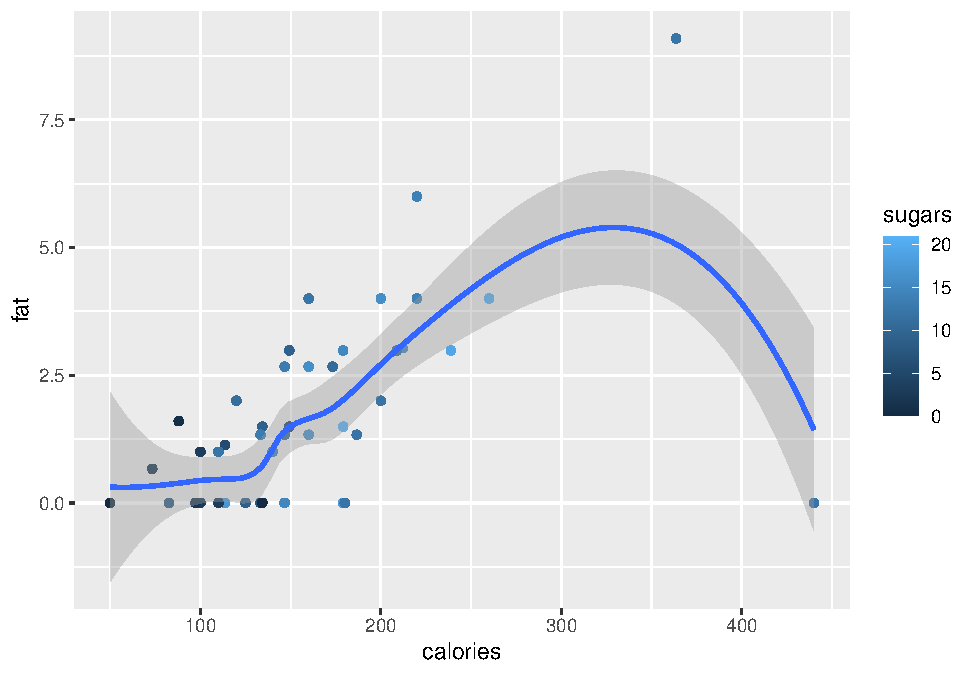
\includegraphics[keepaspectratio]{10-graphics2_files/figure-latex/ggplotScatter3-1.pdf}}

The smooth function can also be a linear regression line.

\begin{Shaded}
\begin{Highlighting}[]
\FunctionTok{ggplot}\NormalTok{(}\AttributeTok{data =}\NormalTok{ cereal, }
       \AttributeTok{mapping =} \FunctionTok{aes}\NormalTok{(}\AttributeTok{x =}\NormalTok{ calories, }\AttributeTok{y =}\NormalTok{ fat)) }\SpecialCharTok{+} 
       \FunctionTok{geom\_point}\NormalTok{(}\AttributeTok{mapping =} \FunctionTok{aes}\NormalTok{(}\AttributeTok{colour =}\NormalTok{ sugars)) }\SpecialCharTok{+}
       \FunctionTok{geom\_smooth}\NormalTok{(}\AttributeTok{method =} \StringTok{"lm"}\NormalTok{)}
\CommentTok{\#\textgreater{} \textasciigrave{}geom\_smooth()\textasciigrave{} using formula = \textquotesingle{}y \textasciitilde{} x\textquotesingle{}}
\end{Highlighting}
\end{Shaded}

\pandocbounded{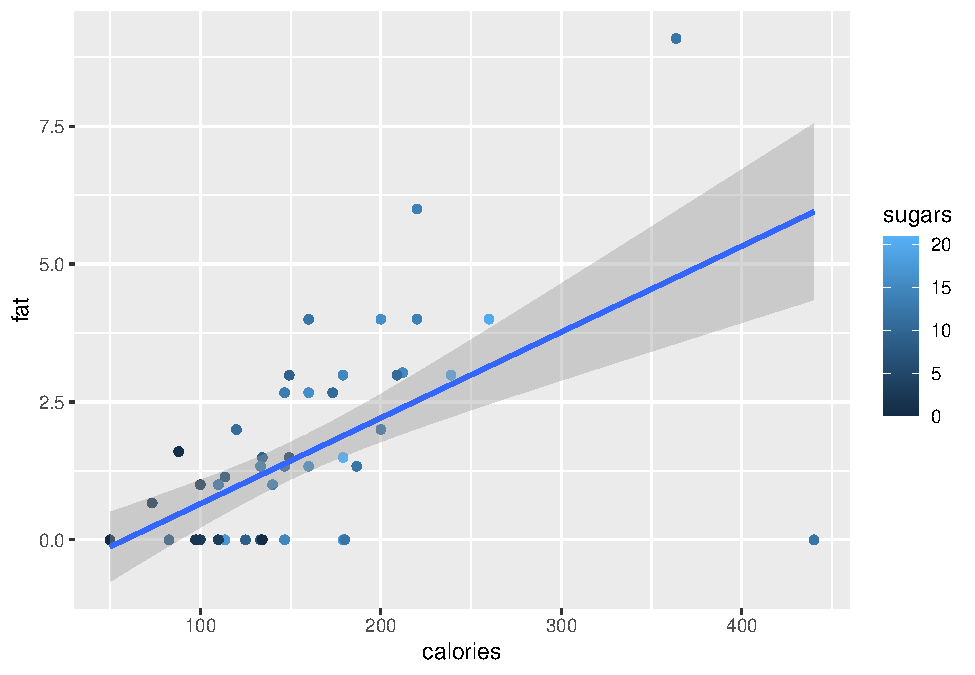
\includegraphics[keepaspectratio]{10-graphics2_files/figure-latex/ggplotScatter4-1.pdf}}

To add different sizes and shapes according to \texttt{shelf} and \texttt{mfr}, respectively, we need the command

\begin{Shaded}
\begin{Highlighting}[]
\FunctionTok{ggplot}\NormalTok{(}\AttributeTok{data =}\NormalTok{ cereal, }
       \AttributeTok{mapping =} \FunctionTok{aes}\NormalTok{(}\AttributeTok{x =}\NormalTok{ calories, }\AttributeTok{y =}\NormalTok{ fat)) }\SpecialCharTok{+} 
       \FunctionTok{geom\_point}\NormalTok{(}\AttributeTok{mapping =} \FunctionTok{aes}\NormalTok{(}\AttributeTok{colour =}\NormalTok{ sugars, }
                                \AttributeTok{shape =}\NormalTok{ mfr, }
                                \AttributeTok{size =} \FunctionTok{factor}\NormalTok{(shelf)))}
\CommentTok{\#\textgreater{} Warning: Using size for a discrete variable is not advised.}
\end{Highlighting}
\end{Shaded}

\pandocbounded{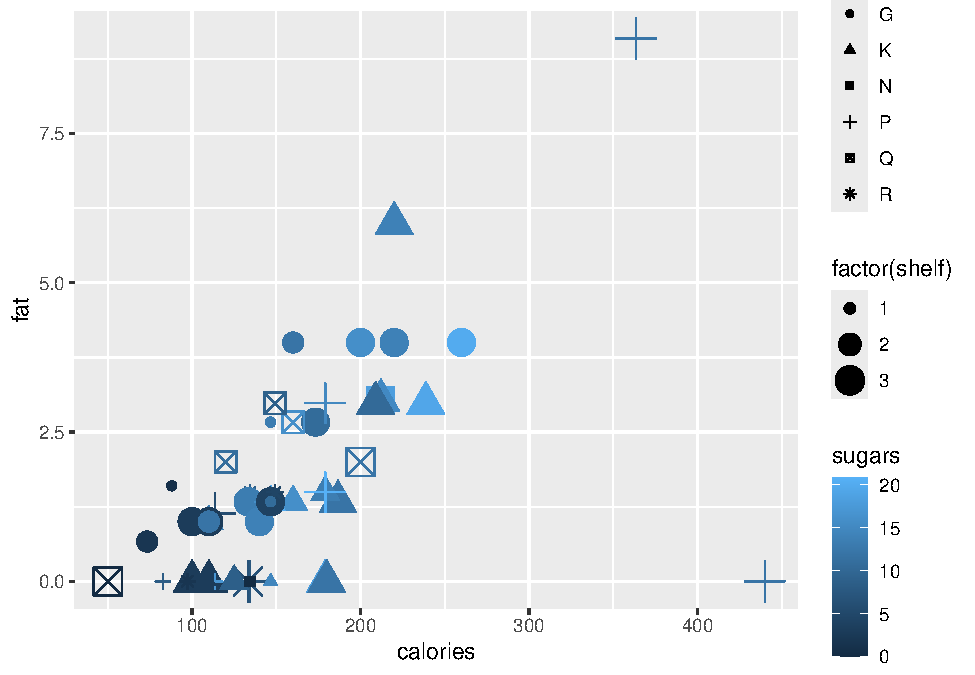
\includegraphics[keepaspectratio]{10-graphics2_files/figure-latex/ggplotScatter5-1.pdf}}

Finally, since there are multiple observations with zero fat, we want to jitter the observations in the vertical direction with a random amount in the interval \(±0.05\).

\begin{Shaded}
\begin{Highlighting}[]
\FunctionTok{ggplot}\NormalTok{(}\AttributeTok{data=}\NormalTok{cereal, }
       \AttributeTok{mapping =} \FunctionTok{aes}\NormalTok{(}\AttributeTok{x =}\NormalTok{ calories, }\AttributeTok{y =}\NormalTok{ fat)) }\SpecialCharTok{+} 
       \FunctionTok{geom\_point}\NormalTok{(}\AttributeTok{mapping=}\FunctionTok{aes}\NormalTok{(}\AttributeTok{colour =}\NormalTok{ sugars),}
                              \AttributeTok{shape =} \StringTok{"cross"}\NormalTok{,}
                              \AttributeTok{position =} \FunctionTok{position\_jitter}\NormalTok{(}\AttributeTok{height=}\FloatTok{0.05}\NormalTok{))}
\end{Highlighting}
\end{Shaded}

\pandocbounded{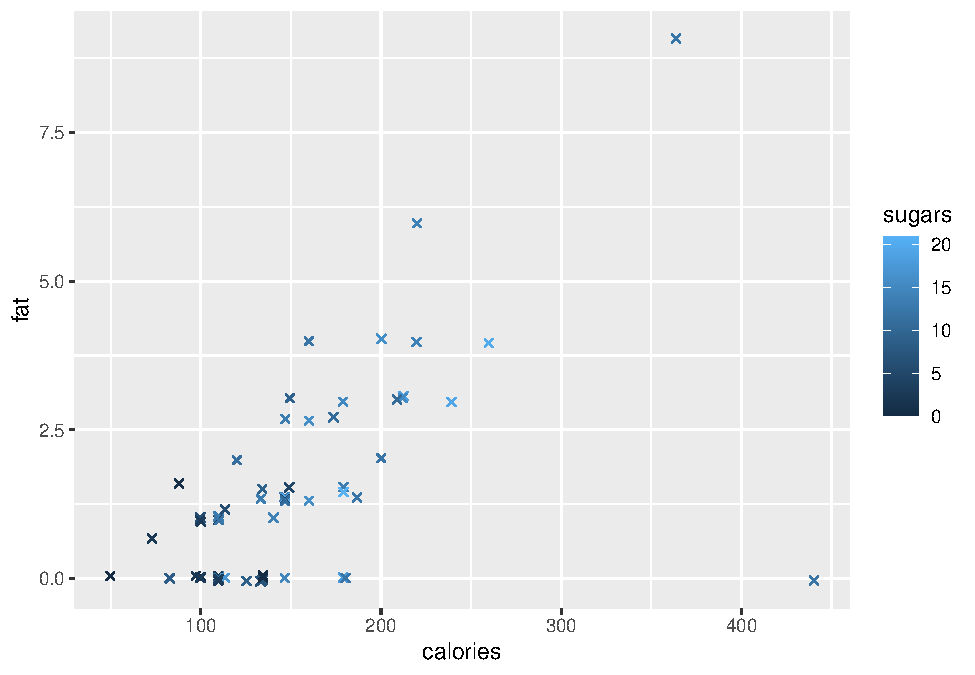
\includegraphics[keepaspectratio]{10-graphics2_files/figure-latex/ggplotScatter6-1.pdf}}

The \texttt{geom\_text()} and \texttt{geom\_label()} functions are useful to replace plotting characters with sample names or a specified label.

\begin{Shaded}
\begin{Highlighting}[]
\FunctionTok{ggplot}\NormalTok{(}\AttributeTok{data =}\NormalTok{ cereal, }
       \AttributeTok{mapping =} \FunctionTok{aes}\NormalTok{(}\AttributeTok{x =}\NormalTok{ calories, }\AttributeTok{y =}\NormalTok{ fat)) }\SpecialCharTok{+} 
       \FunctionTok{geom\_text}\NormalTok{(}\AttributeTok{mapping =} \FunctionTok{aes}\NormalTok{(}\AttributeTok{label=}\NormalTok{mfr))}
\end{Highlighting}
\end{Shaded}

\pandocbounded{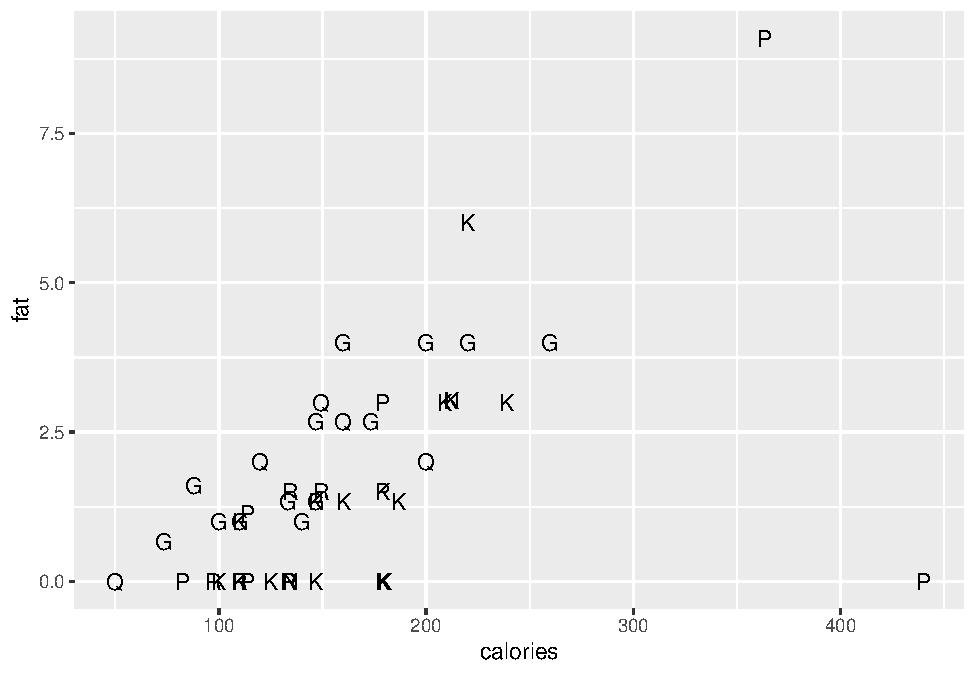
\includegraphics[keepaspectratio]{10-graphics2_files/figure-latex/ggplotScatter7-1.pdf}}

\begin{Shaded}
\begin{Highlighting}[]

\FunctionTok{ggplot}\NormalTok{(}\AttributeTok{data =}\NormalTok{ cereal, }
       \AttributeTok{mapping =} \FunctionTok{aes}\NormalTok{(}\AttributeTok{x =}\NormalTok{ calories, }\AttributeTok{y =}\NormalTok{ fat)) }\SpecialCharTok{+} 
       \FunctionTok{geom\_text}\NormalTok{(}\AttributeTok{mapping=}\FunctionTok{aes}\NormalTok{(}\AttributeTok{label=}\NormalTok{mfr), }\AttributeTok{check\_overlap=}\NormalTok{T)}
\end{Highlighting}
\end{Shaded}

\pandocbounded{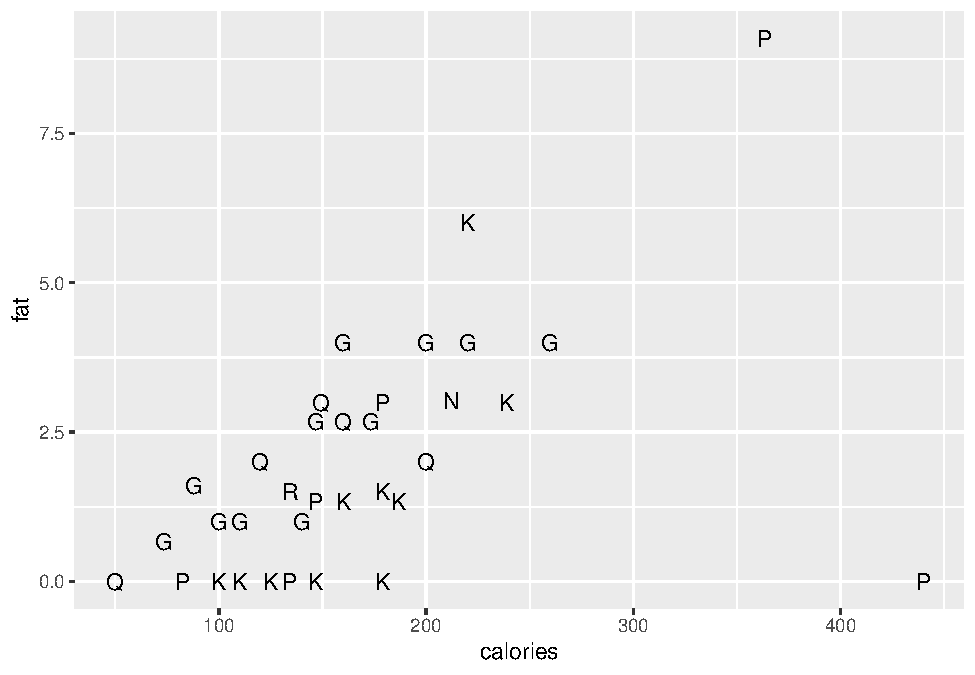
\includegraphics[keepaspectratio]{10-graphics2_files/figure-latex/ggplotScatter7-2.pdf}}

\begin{Shaded}
\begin{Highlighting}[]

\FunctionTok{ggplot}\NormalTok{(}\AttributeTok{data =}\NormalTok{ cereal, }
       \AttributeTok{mapping =} \FunctionTok{aes}\NormalTok{(}\AttributeTok{x =}\NormalTok{ calories, }\AttributeTok{y =}\NormalTok{ fat)) }\SpecialCharTok{+} 
       \FunctionTok{geom\_label}\NormalTok{(}\AttributeTok{mapping =} \FunctionTok{aes}\NormalTok{(}\AttributeTok{label=}\NormalTok{mfr))}
\end{Highlighting}
\end{Shaded}

\pandocbounded{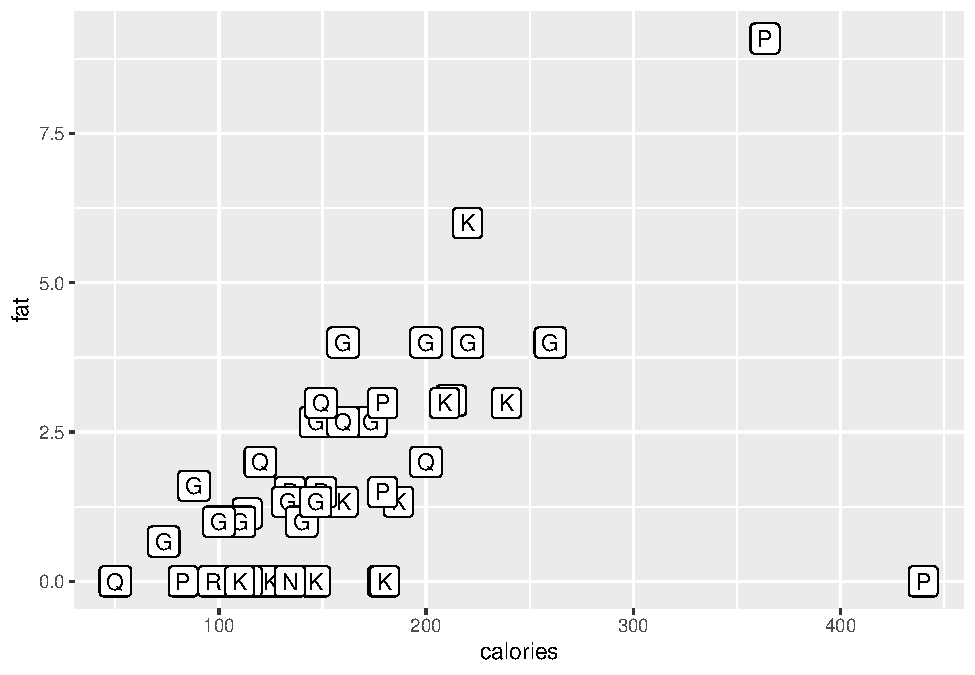
\includegraphics[keepaspectratio]{10-graphics2_files/figure-latex/ggplotScatter7-3.pdf}}

\subsection{Dotplot}\label{dotplot}

Below a simple dotplot of the carbo variable followed by another dotplot with several tweaks in presentation.

\begin{Shaded}
\begin{Highlighting}[]
\FunctionTok{ggplot}\NormalTok{ (}\AttributeTok{data =}\NormalTok{ cereal, }\AttributeTok{mapping =} \FunctionTok{aes}\NormalTok{(}\AttributeTok{x =}\NormalTok{ carbo)) }\SpecialCharTok{+} 
        \FunctionTok{geom\_dotplot}\NormalTok{()  }
\CommentTok{\#\textgreater{} Bin width defaults to 1/30 of the range of the data. Pick}
\CommentTok{\#\textgreater{} better value with \textasciigrave{}binwidth\textasciigrave{}.}
\end{Highlighting}
\end{Shaded}

\pandocbounded{\includegraphics[keepaspectratio]{10-graphics2_files/figure-latex/ggplotDot-1.pdf}}

\begin{Shaded}
\begin{Highlighting}[]

\FunctionTok{ggplot}\NormalTok{ (}\AttributeTok{data =}\NormalTok{ cereal, }\AttributeTok{mapping =} \FunctionTok{aes}\NormalTok{(}\AttributeTok{x =}\NormalTok{ carbo)) }\SpecialCharTok{+} 
        \FunctionTok{geom\_dotplot}\NormalTok{(}\AttributeTok{binwidth =} \DecValTok{2}\NormalTok{, }\AttributeTok{stackdir =} \StringTok{"center"}\NormalTok{, }
                     \AttributeTok{stackratio =} \FloatTok{0.8}\NormalTok{, }\AttributeTok{dotsize =} \FloatTok{1.2}\NormalTok{)  }
\end{Highlighting}
\end{Shaded}

\pandocbounded{\includegraphics[keepaspectratio]{10-graphics2_files/figure-latex/ggplotDot-2.pdf}}

\subsection{Boxplot}\label{boxplot}

The \texttt{geom\_boxplot()} function allows us to make a simple boxplot. However, below we make several boxplots according to vitamin enrichment and overlay the observed data.

\begin{Shaded}
\begin{Highlighting}[]
\FunctionTok{ggplot}\NormalTok{ (}\AttributeTok{data =}\NormalTok{ cereal, }
        \AttributeTok{mapping =} \FunctionTok{aes}\NormalTok{(}\AttributeTok{x =}\NormalTok{ vitamins, }\AttributeTok{y =}\NormalTok{ sodium)) }\SpecialCharTok{+}
        \FunctionTok{geom\_boxplot}\NormalTok{() }\SpecialCharTok{+} \FunctionTok{geom\_jitter}\NormalTok{()}
\end{Highlighting}
\end{Shaded}

\pandocbounded{\includegraphics[keepaspectratio]{10-graphics2_files/figure-latex/ggplotBoxplot-1.pdf}}

\begin{Shaded}
\begin{Highlighting}[]

\FunctionTok{ggplot}\NormalTok{ (}\AttributeTok{data =}\NormalTok{ cereal, }
        \AttributeTok{mapping =} \FunctionTok{aes}\NormalTok{(}\AttributeTok{x =}\NormalTok{ vitamins, }\AttributeTok{y =}\NormalTok{ sodium)) }\SpecialCharTok{+}
        \FunctionTok{geom\_boxplot}\NormalTok{() }\SpecialCharTok{+} \FunctionTok{geom\_jitter}\NormalTok{()}
\end{Highlighting}
\end{Shaded}

\pandocbounded{\includegraphics[keepaspectratio]{10-graphics2_files/figure-latex/ggplotBoxplot-2.pdf}}

\subsection{Line plot}\label{line-plot}

To illustrate plotting lines with \texttt{ggplot2} we will create a small data set \(y_a=log(x)\)⁡ and \(y_b=2log(x)\) with \(0 < x< 1\).

\begin{Shaded}
\begin{Highlighting}[]
\NormalTok{x }\OtherTok{\textless{}{-}} \FunctionTok{seq}\NormalTok{(}\AttributeTok{from =} \FloatTok{0.01}\NormalTok{, }\AttributeTok{to =} \FloatTok{0.99}\NormalTok{, }\AttributeTok{len =} \DecValTok{100}\NormalTok{) }
\NormalTok{y }\OtherTok{\textless{}{-}} \FunctionTok{c}\NormalTok{(}\FunctionTok{log}\NormalTok{(x), }\DecValTok{2} \SpecialCharTok{*} \FunctionTok{log}\NormalTok{(x))   }
\NormalTok{z }\OtherTok{\textless{}{-}} \FunctionTok{rep}\NormalTok{(}\FunctionTok{c}\NormalTok{(}\StringTok{"a"}\NormalTok{, }\StringTok{"b"}\NormalTok{), }\AttributeTok{each =} \DecValTok{100}\NormalTok{) }

\NormalTok{dat }\OtherTok{\textless{}{-}} \FunctionTok{tibble}\NormalTok{(}\AttributeTok{x=}\FunctionTok{rep}\NormalTok{(x,}\DecValTok{2}\NormalTok{), y, z) }
\NormalTok{dat}
\CommentTok{\#\textgreater{} \# A tibble: 200 x 3}
\CommentTok{\#\textgreater{}         x     y z    }
\CommentTok{\#\textgreater{}     \textless{}dbl\textgreater{} \textless{}dbl\textgreater{} \textless{}chr\textgreater{}}
\CommentTok{\#\textgreater{}  1 0.01   {-}4.61 a    }
\CommentTok{\#\textgreater{}  2 0.0199 {-}3.92 a    }
\CommentTok{\#\textgreater{}  3 0.0298 {-}3.51 a    }
\CommentTok{\#\textgreater{}  4 0.0397 {-}3.23 a    }
\CommentTok{\#\textgreater{}  5 0.0496 {-}3.00 a    }
\CommentTok{\#\textgreater{}  6 0.0595 {-}2.82 a    }
\CommentTok{\#\textgreater{}  7 0.0694 {-}2.67 a    }
\CommentTok{\#\textgreater{}  8 0.0793 {-}2.53 a    }
\CommentTok{\#\textgreater{}  9 0.0892 {-}2.42 a    }
\CommentTok{\#\textgreater{} 10 0.0991 {-}2.31 a    }
\CommentTok{\#\textgreater{} \# i 190 more rows}

\FunctionTok{ggplot}\NormalTok{(dat, }\FunctionTok{aes}\NormalTok{(}\AttributeTok{x =}\NormalTok{ x, }\AttributeTok{y =}\NormalTok{ y)) }\SpecialCharTok{+} 
       \FunctionTok{geom\_line}\NormalTok{(}\FunctionTok{aes}\NormalTok{(}\AttributeTok{colour =}\NormalTok{ z))}
\end{Highlighting}
\end{Shaded}

\pandocbounded{\includegraphics[keepaspectratio]{10-graphics2_files/figure-latex/ggplotLine-1.pdf}}

\subsection{Density estimates}\label{density-estimates}

Non-parametric density estimates are useful to summarise the distribution of data. For a single variable, the \texttt{geom\_density()} function produces a density estimate (see section \ref{density}). Here we illustrate the use of the two-dimensional density estimate with the function \texttt{geom\_density\_2d()} and the Old Faithful data from package \texttt{datasets}. Note that the call to \texttt{ggplot()} is written to the object \texttt{p1}. The content of \texttt{p1} is the plot. Assigning the name \texttt{p1} to the plot prevents having to retype the full call for every subsequent execution.

\begin{Shaded}
\begin{Highlighting}[]
\NormalTok{p1 }\OtherTok{\textless{}{-}} \FunctionTok{ggplot}\NormalTok{ (faithful, }
              \FunctionTok{aes}\NormalTok{(}\AttributeTok{x =}\NormalTok{ eruptions, }\AttributeTok{y =}\NormalTok{ waiting)) }\SpecialCharTok{+}
              \FunctionTok{geom\_point}\NormalTok{() }\SpecialCharTok{+} \FunctionTok{xlim}\NormalTok{(}\FloatTok{0.5}\NormalTok{,}\DecValTok{5}\NormalTok{) }\SpecialCharTok{+} \FunctionTok{ylim}\NormalTok{(}\DecValTok{40}\NormalTok{,}\DecValTok{110}\NormalTok{)}

\NormalTok{p1}
\CommentTok{\#\textgreater{} Warning: Removed 3 rows containing missing values or values outside}
\CommentTok{\#\textgreater{} the scale range (\textasciigrave{}geom\_point()\textasciigrave{}).}
\end{Highlighting}
\end{Shaded}

\pandocbounded{\includegraphics[keepaspectratio]{10-graphics2_files/figure-latex/ggplotDensity-1.pdf}}

\begin{Shaded}
\begin{Highlighting}[]
\NormalTok{p1 }\SpecialCharTok{+} \FunctionTok{geom\_density\_2d}\NormalTok{()}
\CommentTok{\#\textgreater{} Warning: Removed 3 rows containing non{-}finite outside the scale}
\CommentTok{\#\textgreater{} range (\textasciigrave{}stat\_density2d()\textasciigrave{}).}
\CommentTok{\#\textgreater{} Removed 3 rows containing missing values or values outside}
\CommentTok{\#\textgreater{} the scale range (\textasciigrave{}geom\_point()\textasciigrave{}).}
\end{Highlighting}
\end{Shaded}

\pandocbounded{\includegraphics[keepaspectratio]{10-graphics2_files/figure-latex/ggplotDensity-2.pdf}}

In the above examples, the geometry is specified, without any specification of statistical transformations. Although not specified explicitly, statistical transformations are performed. For instance in the barplot above, the \texttt{stat\_count()} is the default for \texttt{geom\_bar()} to determine the frequencies plotted on the vertical axis. In most instances, the default \texttt{stat\_xxx()} function is appropriate for the particular \texttt{geom\_yyy()} function and specifying other statistical transformations could lead to non-sensicle calls. In most calls to \texttt{ggplot()}, the default \texttt{stat\_xxx()} is appropriate and not explicitly specified. Below, we look at a few exceptions.

\subsection{Empirical cumulative distribution function}\label{empirical-cumulative-distribution-function}

The empirical cumulative distribution function also provide details on the shape of the distribution underlying the observations and can be plotted with \texttt{stat\_ecdf()}.

\begin{Shaded}
\begin{Highlighting}[]
\NormalTok{n.}\FloatTok{1.1} \OtherTok{\textless{}{-}} \FunctionTok{rnorm}\NormalTok{(}\DecValTok{100}\NormalTok{, }\DecValTok{1}\NormalTok{, }\DecValTok{1}\NormalTok{)}
\NormalTok{F.}\FloatTok{4.9} \OtherTok{\textless{}{-}} \FunctionTok{rf}\NormalTok{(}\DecValTok{100}\NormalTok{, }\DecValTok{4}\NormalTok{,}\DecValTok{9}\NormalTok{)}
\NormalTok{dat }\OtherTok{\textless{}{-}} \FunctionTok{tibble}\NormalTok{(n.}\FloatTok{1.1}\NormalTok{,F.}\FloatTok{4.9}\NormalTok{)}
\NormalTok{dat2 }\OtherTok{\textless{}{-}} \FunctionTok{pivot\_longer}\NormalTok{(dat, }\AttributeTok{cols =} \FunctionTok{everything}\NormalTok{())}
\FunctionTok{ggplot}\NormalTok{ (dat, }\FunctionTok{aes}\NormalTok{(}\AttributeTok{x=}\NormalTok{n.}\FloatTok{1.1}\NormalTok{)) }\SpecialCharTok{+} \FunctionTok{stat\_ecdf}\NormalTok{()}
\end{Highlighting}
\end{Shaded}

\pandocbounded{\includegraphics[keepaspectratio]{10-graphics2_files/figure-latex/ggplotEcdf-1.pdf}}

\begin{Shaded}
\begin{Highlighting}[]
\FunctionTok{ggplot}\NormalTok{ (dat2, }\FunctionTok{aes}\NormalTok{(}\AttributeTok{x=}\NormalTok{value, }\AttributeTok{colour =}\NormalTok{ name)) }\SpecialCharTok{+} \FunctionTok{stat\_ecdf}\NormalTok{()}
\end{Highlighting}
\end{Shaded}

\pandocbounded{\includegraphics[keepaspectratio]{10-graphics2_files/figure-latex/ggplotEcdf-2.pdf}}

\subsection{Mathematical functions}\label{mathematical-functions}

Any function \(f(x)\) can be plotted, or added to a plot with \texttt{stat\_function()}. First we will plot the function \(f(x)=2e^xcos⁡(x)\).

\begin{Shaded}
\begin{Highlighting}[]
\NormalTok{p2 }\OtherTok{\textless{}{-}} \FunctionTok{ggplot}\NormalTok{() }\SpecialCharTok{+} \FunctionTok{xlim}\NormalTok{(}\SpecialCharTok{{-}}\DecValTok{5}\NormalTok{,}\DecValTok{5}\NormalTok{)}
\NormalTok{p2 }\SpecialCharTok{+} \FunctionTok{geom\_function}\NormalTok{(}\AttributeTok{fun =} \ControlFlowTok{function}\NormalTok{(x) }\DecValTok{2}\SpecialCharTok{*}\FunctionTok{exp}\NormalTok{(x)}\SpecialCharTok{*}\FunctionTok{cos}\NormalTok{(x))}
\end{Highlighting}
\end{Shaded}

\pandocbounded{\includegraphics[keepaspectratio]{10-graphics2_files/figure-latex/ggplotfx-1.pdf}}

Next we will compare our empirical cumulative distribution function, to the cumulative distribution functions of a Poisson and normal distribution. (Remember, the normal distribution provides an approximation to the Poisson).

\begin{Shaded}
\begin{Highlighting}[]
\NormalTok{x3 }\OtherTok{\textless{}{-}} \FunctionTok{rpois}\NormalTok{(}\DecValTok{100}\NormalTok{, }\DecValTok{5}\NormalTok{)}
\NormalTok{dat3 }\OtherTok{\textless{}{-}} \FunctionTok{tibble}\NormalTok{(x3)}
\FunctionTok{ggplot}\NormalTok{ (dat3, }\FunctionTok{aes}\NormalTok{(}\AttributeTok{x =}\NormalTok{ x3)) }\SpecialCharTok{+} \FunctionTok{stat\_ecdf}\NormalTok{() }\SpecialCharTok{+} 
        \FunctionTok{geom\_function}\NormalTok{(}\AttributeTok{fun =}\NormalTok{ ppois,    }
                \AttributeTok{args=}\FunctionTok{list}\NormalTok{(}\AttributeTok{lambda=}\FunctionTok{mean}\NormalTok{(x3)), }\AttributeTok{col=}\StringTok{"blue"}\NormalTok{) }\SpecialCharTok{+}
        \FunctionTok{geom\_function}\NormalTok{(}\AttributeTok{fun =}\NormalTok{ pnorm, }
               \AttributeTok{args=}\FunctionTok{list}\NormalTok{(}\AttributeTok{mean=}\FunctionTok{mean}\NormalTok{(x3), }\AttributeTok{sd=}\FunctionTok{sqrt}\NormalTok{(}\FunctionTok{mean}\NormalTok{(x3))), }
               \AttributeTok{col=}\StringTok{"red"}\NormalTok{)}
\end{Highlighting}
\end{Shaded}

\pandocbounded{\includegraphics[keepaspectratio]{10-graphics2_files/figure-latex/gglotfx2-1.pdf}}

\subsection{\texorpdfstring{\texttt{after\_stat()} function}{after\_stat() function}}\label{after_stat-function}

When constructing a histogram, the frequencies appear on the vertical axis. These frequencies are the output of the function \texttt{stat\_bin()} which means they are not available up front in the data set itself. The \texttt{after\_stat()} function allows us to use the computed variables, for instance to scale the histogram to area \(=1\) in order to compare the observed distribution to a theoretical probability density function.

\begin{Shaded}
\begin{Highlighting}[]
\NormalTok{x4 }\OtherTok{\textless{}{-}} \FunctionTok{rgamma}\NormalTok{(}\DecValTok{1000}\NormalTok{, }\DecValTok{5}\NormalTok{, }\DecValTok{3}\NormalTok{)}
\NormalTok{dat4 }\OtherTok{\textless{}{-}} \FunctionTok{tibble}\NormalTok{(x4)}
\FunctionTok{ggplot}\NormalTok{ (dat4, }\FunctionTok{aes}\NormalTok{(x4)) }\SpecialCharTok{+} \FunctionTok{geom\_histogram}\NormalTok{()}
\CommentTok{\#\textgreater{} \textasciigrave{}stat\_bin()\textasciigrave{} using \textasciigrave{}bins = 30\textasciigrave{}. Pick better value with}
\CommentTok{\#\textgreater{} \textasciigrave{}binwidth\textasciigrave{}.}
\end{Highlighting}
\end{Shaded}

\pandocbounded{\includegraphics[keepaspectratio]{10-graphics2_files/figure-latex/ggplotAfterstat-1.pdf}}

\begin{Shaded}
\begin{Highlighting}[]
  
\FunctionTok{ggplot}\NormalTok{(dat4, }\FunctionTok{aes}\NormalTok{(x4)) }\SpecialCharTok{+}
       \FunctionTok{geom\_histogram}\NormalTok{(}\FunctionTok{aes}\NormalTok{(}\AttributeTok{y=}\FunctionTok{after\_stat}\NormalTok{(density)), }
                      \AttributeTok{fill=}\StringTok{"pink"}\NormalTok{) }\SpecialCharTok{+}
       \FunctionTok{geom\_function}\NormalTok{ (}\AttributeTok{fun =}\NormalTok{ dgamma, }
                      \AttributeTok{args=}\FunctionTok{list}\NormalTok{(}\AttributeTok{shape =} \DecValTok{5}\NormalTok{, }\AttributeTok{rate =} \DecValTok{3}\NormalTok{))}
\CommentTok{\#\textgreater{} \textasciigrave{}stat\_bin()\textasciigrave{} using \textasciigrave{}bins = 30\textasciigrave{}. Pick better value with}
\CommentTok{\#\textgreater{} \textasciigrave{}binwidth\textasciigrave{}.}
\end{Highlighting}
\end{Shaded}

\pandocbounded{\includegraphics[keepaspectratio]{10-graphics2_files/figure-latex/ggplotAfterstat-2.pdf}}

\subsection{Scales}\label{scales}

The scales link the aesthetic attributes such as colours, plotting characters, line types, axis scales etc. to the data. Implicitly, in all the calls above, default scales are specified. Should we wish to change the defaults, the scales need to be specified explicitly.

In the call

\begin{Shaded}
\begin{Highlighting}[]
\FunctionTok{ggplot}\NormalTok{(}\AttributeTok{data =}\NormalTok{ cereal, }
       \AttributeTok{mapping =} \FunctionTok{aes}\NormalTok{(}\AttributeTok{x =}\NormalTok{ calories, }\AttributeTok{y =}\NormalTok{ fat)) }\SpecialCharTok{+} 
       \FunctionTok{geom\_point}\NormalTok{(}\AttributeTok{mapping =} \FunctionTok{aes}\NormalTok{(}\AttributeTok{colour =}\NormalTok{ mfr))}
\end{Highlighting}
\end{Shaded}

\pandocbounded{\includegraphics[keepaspectratio]{10-graphics2_files/figure-latex/ggplotScales-1.pdf}}

different colours are assigned to the points, based on the content of \texttt{mfr}. Since \texttt{mfr} is a categorical variable with six levels, the first six default colours are used. The user can specify their own colour selection with the function \texttt{scale\_colour\_manual()}. However, the Brewer palettes are convenient colour schemes designed by Cynthia Brewer as described at
\url{http://colorbrewer2.org}. Below a qualitative scale is used according to the levels of \texttt{mfr}.

\begin{Shaded}
\begin{Highlighting}[]
\FunctionTok{ggplot}\NormalTok{(}\AttributeTok{data =}\NormalTok{ cereal, }
       \AttributeTok{mapping =} \FunctionTok{aes}\NormalTok{(}\AttributeTok{x =}\NormalTok{ calories, }\AttributeTok{y =}\NormalTok{ fat)) }\SpecialCharTok{+} 
       \FunctionTok{geom\_point}\NormalTok{(}\AttributeTok{mapping =} \FunctionTok{aes}\NormalTok{(}\AttributeTok{colour =}\NormalTok{ mfr)) }\SpecialCharTok{+}
       \FunctionTok{scale\_colour\_brewer}\NormalTok{(}\AttributeTok{type =} \StringTok{"qual"}\NormalTok{)}
\end{Highlighting}
\end{Shaded}

\pandocbounded{\includegraphics[keepaspectratio]{10-graphics2_files/figure-latex/ggplotScales2-1.pdf}}

Next, we will define our own gradient fill scaling for use with the continuous variable \texttt{sugars}. The default scale ranges from light blue to dark blue.

\begin{Shaded}
\begin{Highlighting}[]
\FunctionTok{ggplot}\NormalTok{(}\AttributeTok{data =}\NormalTok{ cereal, }
       \AttributeTok{mapping =} \FunctionTok{aes}\NormalTok{(}\AttributeTok{x =}\NormalTok{ calories, }\AttributeTok{y =}\NormalTok{ fat)) }\SpecialCharTok{+} 
       \FunctionTok{geom\_point}\NormalTok{(}\AttributeTok{mapping =} \FunctionTok{aes}\NormalTok{(}\AttributeTok{colour =}\NormalTok{ sugars))}
\end{Highlighting}
\end{Shaded}

\pandocbounded{\includegraphics[keepaspectratio]{10-graphics2_files/figure-latex/ggplotScales3-1.pdf}}

The built in colour palettes \texttt{hcl.colors}, \texttt{hcl.pals}, \texttt{rainbow}, \texttt{heat.colors}, \texttt{terrain.colors}, \texttt{topo.colors} and \texttt{cm.colors} can be selected with the function \texttt{scale\_colour\_gradientn()} or \texttt{scale\_fill\_gradientn()}.

\begin{Shaded}
\begin{Highlighting}[]
\FunctionTok{ggplot}\NormalTok{(}\AttributeTok{data =}\NormalTok{ cereal, }
       \AttributeTok{mapping =} \FunctionTok{aes}\NormalTok{(}\AttributeTok{x =}\NormalTok{ calories, }\AttributeTok{y =}\NormalTok{ fat)) }\SpecialCharTok{+} 
       \FunctionTok{geom\_point}\NormalTok{(}\AttributeTok{mapping =} \FunctionTok{aes}\NormalTok{(}\AttributeTok{colour =}\NormalTok{ sugars))}\SpecialCharTok{+}
       \FunctionTok{scale\_colour\_gradientn}\NormalTok{(}\AttributeTok{colours =} \FunctionTok{rainbow}\NormalTok{(}\DecValTok{21}\NormalTok{))}
\end{Highlighting}
\end{Shaded}

\pandocbounded{\includegraphics[keepaspectratio]{10-graphics2_files/figure-latex/ggplotScales4-1.pdf}}

The functions \texttt{scale\_colour\_gradient()} and \texttt{scale\_fill\_gradient()} allows the user to specify a two-colour gradient scale while \texttt{scale\_colour\_gradient2()} and \texttt{scale\_fill\_gradient2()} allows for specification of a three-colour gradient scale.

\begin{Shaded}
\begin{Highlighting}[]
\FunctionTok{ggplot}\NormalTok{(}\AttributeTok{data =}\NormalTok{ cereal, }
       \AttributeTok{mapping =} \FunctionTok{aes}\NormalTok{(}\AttributeTok{x =}\NormalTok{ calories, }\AttributeTok{y =}\NormalTok{ fat)) }\SpecialCharTok{+} 
       \FunctionTok{geom\_point}\NormalTok{(}\AttributeTok{mapping =} \FunctionTok{aes}\NormalTok{(}\AttributeTok{colour =}\NormalTok{ sugars))}\SpecialCharTok{+}
       \FunctionTok{scale\_colour\_gradient}\NormalTok{(}\AttributeTok{low =} \StringTok{"black"}\NormalTok{, }
                             \AttributeTok{high =} \StringTok{"orange"}\NormalTok{)}
\end{Highlighting}
\end{Shaded}

\pandocbounded{\includegraphics[keepaspectratio]{10-graphics2_files/figure-latex/ggplotScales5-1.pdf}}

In a final example of scales we will change the vertical axis to a log scale while changing the axis markers on the horizontal scale.

\begin{Shaded}
\begin{Highlighting}[]
\FunctionTok{ggplot}\NormalTok{(}\AttributeTok{data =}\NormalTok{ cereal, }
       \AttributeTok{mapping =} \FunctionTok{aes}\NormalTok{(}\AttributeTok{x =}\NormalTok{ calories, }\AttributeTok{y =}\NormalTok{ fat)) }\SpecialCharTok{+} 
       \FunctionTok{geom\_point}\NormalTok{(}\AttributeTok{mapping =} \FunctionTok{aes}\NormalTok{(}\AttributeTok{colour =}\NormalTok{ sugars))}\SpecialCharTok{+}
       \FunctionTok{scale\_colour\_gradient}\NormalTok{(}\AttributeTok{low =} \StringTok{"black"}\NormalTok{, }
                             \AttributeTok{high =} \StringTok{"orange"}\NormalTok{) }\SpecialCharTok{+}
       \FunctionTok{scale\_x\_continuous}\NormalTok{(}\AttributeTok{breaks =} \FunctionTok{seq}\NormalTok{(}\AttributeTok{from =} \DecValTok{50}\NormalTok{, }\AttributeTok{to =} \DecValTok{450}\NormalTok{, }\AttributeTok{by =} \DecValTok{50}\NormalTok{)) }\SpecialCharTok{+} 
       \FunctionTok{scale\_y\_continuous}\NormalTok{(}\AttributeTok{trans =} \StringTok{"log"}\NormalTok{)}
\CommentTok{\#\textgreater{} Warning in scale\_y\_continuous(trans = "log"): log{-}2.718282}
\CommentTok{\#\textgreater{} transformation introduced infinite values.}
\end{Highlighting}
\end{Shaded}

\pandocbounded{\includegraphics[keepaspectratio]{10-graphics2_files/figure-latex/ggplotScales6-1.pdf}}

\subsection{Coordinates}\label{coordinates}

By default, all the plots we have made are on the Cartesian axes. One alternative would be to use a polar coordinate system.

\begin{Shaded}
\begin{Highlighting}[]
\CommentTok{\# Hadley\textquotesingle{}s favourite pie chart}
\NormalTok{df }\OtherTok{\textless{}{-}} \FunctionTok{data.frame}\NormalTok{(}
  \AttributeTok{variable =} \FunctionTok{c}\NormalTok{(}\StringTok{"does not resemble"}\NormalTok{, }\StringTok{"resembles"}\NormalTok{),}
  \AttributeTok{value =} \FunctionTok{c}\NormalTok{(}\DecValTok{20}\NormalTok{, }\DecValTok{80}\NormalTok{)}
\NormalTok{)}

\FunctionTok{ggplot}\NormalTok{(df, }\FunctionTok{aes}\NormalTok{(}\AttributeTok{x =} \StringTok{""}\NormalTok{, }\AttributeTok{y =}\NormalTok{ value, }\AttributeTok{fill =}\NormalTok{ variable)) }\SpecialCharTok{+}
       \FunctionTok{geom\_col}\NormalTok{(}\AttributeTok{width =} \DecValTok{1}\NormalTok{) }\SpecialCharTok{+}
       \FunctionTok{scale\_fill\_manual}\NormalTok{(}\AttributeTok{values =} \FunctionTok{c}\NormalTok{(}\StringTok{"red"}\NormalTok{, }\StringTok{"yellow"}\NormalTok{)) }\SpecialCharTok{+}
       \FunctionTok{coord\_polar}\NormalTok{(}\StringTok{"y"}\NormalTok{, }\AttributeTok{start =}\NormalTok{ pi }\SpecialCharTok{/} \DecValTok{3}\NormalTok{) }\SpecialCharTok{+}
       \FunctionTok{labs}\NormalTok{(}\AttributeTok{title =} \StringTok{"Pac man"}\NormalTok{)}
\end{Highlighting}
\end{Shaded}

\pandocbounded{\includegraphics[keepaspectratio]{10-graphics2_files/figure-latex/ggplotCoords-1.pdf}}

To plot the function \(f(\theta)=\theta sin(\theta)\), \(0 \le \theta \le \frac{\pi}{2}\) we need to following code:

\begin{Shaded}
\begin{Highlighting}[]
\NormalTok{theta.vec }\OtherTok{\textless{}{-}} \FunctionTok{seq}\NormalTok{(}\AttributeTok{from =} \DecValTok{0}\NormalTok{, }\AttributeTok{to =}\NormalTok{ pi}\SpecialCharTok{/}\DecValTok{2}\NormalTok{, }\AttributeTok{len =} \DecValTok{200}\NormalTok{)}
\NormalTok{my.dat }\OtherTok{\textless{}{-}} \FunctionTok{tibble}\NormalTok{ (}\AttributeTok{theta =}\NormalTok{ theta.vec,}
                  \AttributeTok{r =}\NormalTok{ theta.vec}\SpecialCharTok{*}\FunctionTok{sin}\NormalTok{(theta.vec))}
\FunctionTok{ggplot}\NormalTok{ (my.dat) }\SpecialCharTok{+} \FunctionTok{geom\_line}\NormalTok{(}\FunctionTok{aes}\NormalTok{(}\AttributeTok{x =}\NormalTok{ theta, }\AttributeTok{y=}\NormalTok{r)) }\SpecialCharTok{+}
                  \FunctionTok{coord\_polar}\NormalTok{(}\AttributeTok{theta =} \StringTok{"x"}\NormalTok{)}
\end{Highlighting}
\end{Shaded}

\pandocbounded{\includegraphics[keepaspectratio]{10-graphics2_files/figure-latex/ggplotCoords2-1.pdf}}

As illustrated in Exercise \ref{Ex6} number 10 it is sometimes essential to keep the aspect ratio in the graphic fixed, usually at \(1:1\). Classical scaling is a method to produce a map from a given matrix of pairwise distances. In the code below, a map (subject to rotation and reflection) of cities in Europe is produce with the function \texttt{cmdscale()}. In order to visually assess intercity distances, it is important to have one unit in the horizontal direction equal to one unit in the vertical direction. This is achieved with \texttt{coord\_fixed\ (ratio\ =\ 1)}.

\begin{Shaded}
\begin{Highlighting}[]
\NormalTok{city.coords }\OtherTok{\textless{}{-}} \FunctionTok{data.frame}\NormalTok{(}\AttributeTok{city=}\FunctionTok{attr}\NormalTok{(eurodist,}\StringTok{"Labels"}\NormalTok{),}
                          \FunctionTok{cmdscale}\NormalTok{(eurodist))}
\FunctionTok{colnames}\NormalTok{(city.coords)[}\DecValTok{2}\SpecialCharTok{:}\DecValTok{3}\NormalTok{] }\OtherTok{\textless{}{-}} \FunctionTok{paste}\NormalTok{(}\StringTok{"dim"}\NormalTok{,}\DecValTok{1}\SpecialCharTok{:}\DecValTok{2}\NormalTok{,}\AttributeTok{sep=}\StringTok{""}\NormalTok{)}
\NormalTok{city.coords }\OtherTok{\textless{}{-}} \FunctionTok{tibble}\NormalTok{(city.coords)}
\FunctionTok{ggplot}\NormalTok{ (city.coords, }\AttributeTok{mapping =} \FunctionTok{aes}\NormalTok{(}\AttributeTok{x =}\NormalTok{ dim1, }\AttributeTok{y =}\NormalTok{ dim2)) }\SpecialCharTok{+}
        \FunctionTok{geom\_text}\NormalTok{(}\AttributeTok{mapping =} \FunctionTok{aes}\NormalTok{(}\AttributeTok{label=}\NormalTok{city)) }\SpecialCharTok{+}
        \FunctionTok{coord\_fixed}\NormalTok{(}\AttributeTok{ratio =} \DecValTok{1}\NormalTok{)         }
\end{Highlighting}
\end{Shaded}

\pandocbounded{\includegraphics[keepaspectratio]{10-graphics2_files/figure-latex/ggplotCoords3-1.pdf}}

\subsection{Facets}\label{facets}

Facets allows for the grouping of the data set into smaller similar data sets. We can plot the \texttt{fat} vs \texttt{calories} for every manufacturer separately.

\begin{Shaded}
\begin{Highlighting}[]
\FunctionTok{ggplot}\NormalTok{(}\AttributeTok{data =}\NormalTok{ cereal, }
       \AttributeTok{mapping =} \FunctionTok{aes}\NormalTok{(}\AttributeTok{x =}\NormalTok{ calories, }\AttributeTok{y =}\NormalTok{ fat)) }\SpecialCharTok{+} 
       \FunctionTok{geom\_point}\NormalTok{() }\SpecialCharTok{+}
       \FunctionTok{facet\_grid}\NormalTok{ (}\FunctionTok{vars}\NormalTok{(mfr))}
\end{Highlighting}
\end{Shaded}

\pandocbounded{\includegraphics[keepaspectratio]{10-graphics2_files/figure-latex/ggplotFacets-1.pdf}}

\begin{Shaded}
\begin{Highlighting}[]

\FunctionTok{ggplot}\NormalTok{(}\AttributeTok{data =}\NormalTok{ cereal, }
       \AttributeTok{mapping =} \FunctionTok{aes}\NormalTok{(}\AttributeTok{x =}\NormalTok{ calories, }\AttributeTok{y =}\NormalTok{ fat)) }\SpecialCharTok{+} 
       \FunctionTok{geom\_point}\NormalTok{() }\SpecialCharTok{+}
       \FunctionTok{facet\_wrap}\NormalTok{ (}\FunctionTok{vars}\NormalTok{(mfr))}
\end{Highlighting}
\end{Shaded}

\pandocbounded{\includegraphics[keepaspectratio]{10-graphics2_files/figure-latex/ggplotFacets-2.pdf}}

Although it does not allow for comparison across plots, each plot can have its own axis range while splitting the data according to two variables.

\begin{Shaded}
\begin{Highlighting}[]
\FunctionTok{ggplot}\NormalTok{(}\AttributeTok{data =}\NormalTok{ cereal, }
       \AttributeTok{mapping =} \FunctionTok{aes}\NormalTok{(}\AttributeTok{x =}\NormalTok{ calories, }\AttributeTok{y =}\NormalTok{ fat)) }\SpecialCharTok{+} 
       \FunctionTok{geom\_point}\NormalTok{() }\SpecialCharTok{+}
       \FunctionTok{facet\_wrap}\NormalTok{ (}\FunctionTok{vars}\NormalTok{(mfr, vitamins), }\AttributeTok{scales =} \StringTok{"free"}\NormalTok{)}
\end{Highlighting}
\end{Shaded}

\pandocbounded{\includegraphics[keepaspectratio]{10-graphics2_files/figure-latex/ggplotFacets2-1.pdf}}

\subsection{Themes}\label{themes}

As mentioned before, themes is disconnected with the data. Themes allow for the formatting of the background, gridlines, titles, etc.

\begin{Shaded}
\begin{Highlighting}[]
\NormalTok{p3 }\OtherTok{\textless{}{-}} \FunctionTok{ggplot}\NormalTok{(}\AttributeTok{data =}\NormalTok{ cereal, }
      \AttributeTok{mapping =} \FunctionTok{aes}\NormalTok{(}\AttributeTok{y =}\NormalTok{ mfr, }\AttributeTok{fill =}\NormalTok{ vitamins)) }\SpecialCharTok{+}   
      \FunctionTok{geom\_bar}\NormalTok{() }\SpecialCharTok{+} 
      \FunctionTok{facet\_wrap}\NormalTok{(}\FunctionTok{vars}\NormalTok{(mfr))}
\NormalTok{p3}
\end{Highlighting}
\end{Shaded}

\pandocbounded{\includegraphics[keepaspectratio]{10-graphics2_files/figure-latex/ggplotThemes-1.pdf}}

\begin{Shaded}
\begin{Highlighting}[]
\NormalTok{p3 }\SpecialCharTok{+} \FunctionTok{theme\_classic}\NormalTok{()}
\end{Highlighting}
\end{Shaded}

\pandocbounded{\includegraphics[keepaspectratio]{10-graphics2_files/figure-latex/ggplotThemes-2.pdf}}

\begin{Shaded}
\begin{Highlighting}[]
\NormalTok{p3 }\SpecialCharTok{+} \FunctionTok{theme\_minimal}\NormalTok{()}
\end{Highlighting}
\end{Shaded}

\pandocbounded{\includegraphics[keepaspectratio]{10-graphics2_files/figure-latex/ggplotThemes-3.pdf}}

\begin{Shaded}
\begin{Highlighting}[]
\NormalTok{p3 }\SpecialCharTok{+} \FunctionTok{theme}\NormalTok{(}\AttributeTok{panel.grid.major =} \FunctionTok{element\_line}\NormalTok{(}\StringTok{"gray"}\NormalTok{, }\AttributeTok{size =} \FloatTok{0.5}\NormalTok{))}
\CommentTok{\#\textgreater{} Warning: The \textasciigrave{}size\textasciigrave{} argument of \textasciigrave{}element\_line()\textasciigrave{} is deprecated as of}
\CommentTok{\#\textgreater{} ggplot2 3.4.0.}
\CommentTok{\#\textgreater{} i Please use the \textasciigrave{}linewidth\textasciigrave{} argument instead.}
\CommentTok{\#\textgreater{} This warning is displayed once every 8 hours.}
\CommentTok{\#\textgreater{} Call \textasciigrave{}lifecycle::last\_lifecycle\_warnings()\textasciigrave{} to see where}
\CommentTok{\#\textgreater{} this warning was generated.}
\end{Highlighting}
\end{Shaded}

\pandocbounded{\includegraphics[keepaspectratio]{10-graphics2_files/figure-latex/ggplotThemes-4.pdf}}

\begin{Shaded}
\begin{Highlighting}[]
\NormalTok{p3 }\SpecialCharTok{+} \FunctionTok{theme}\NormalTok{(}\AttributeTok{axis.text.y =} \FunctionTok{element\_text}\NormalTok{(}\AttributeTok{size =} \DecValTok{18}\NormalTok{))}
\end{Highlighting}
\end{Shaded}

\pandocbounded{\includegraphics[keepaspectratio]{10-graphics2_files/figure-latex/ggplotThemes-5.pdf}}

\begin{Shaded}
\begin{Highlighting}[]
\NormalTok{p3 }\SpecialCharTok{+} \FunctionTok{ggtitle}\NormalTok{(}\StringTok{"Heading"}\NormalTok{) }\SpecialCharTok{+} \FunctionTok{theme}\NormalTok{(}\AttributeTok{plot.title =} \FunctionTok{element\_text}\NormalTok{(}\AttributeTok{family =} \StringTok{"serif"}\NormalTok{))}
\end{Highlighting}
\end{Shaded}

\pandocbounded{\includegraphics[keepaspectratio]{10-graphics2_files/figure-latex/ggplotThemes-6.pdf}}

\begin{Shaded}
\begin{Highlighting}[]

\NormalTok{p4 }\OtherTok{\textless{}{-}} \FunctionTok{ggplot}\NormalTok{(}\AttributeTok{data =}\NormalTok{ cereal, }
             \AttributeTok{mapping =} \FunctionTok{aes}\NormalTok{(}\AttributeTok{x =}\NormalTok{ calories, }\AttributeTok{y =}\NormalTok{ fat)) }\SpecialCharTok{+} 
             \FunctionTok{geom\_point}\NormalTok{(}\AttributeTok{mapping =} \FunctionTok{aes}\NormalTok{(}\AttributeTok{colour =}\NormalTok{ sugars))}
\NormalTok{p4 }\SpecialCharTok{+} \FunctionTok{guides}\NormalTok{(}\AttributeTok{colour =} \FunctionTok{guide\_colourbar}\NormalTok{(}\AttributeTok{barwidth =} \FloatTok{0.25}\NormalTok{, }\AttributeTok{barheight =} \DecValTok{20}\NormalTok{,}
                                        \AttributeTok{nbin=}\DecValTok{100}\NormalTok{))}
\end{Highlighting}
\end{Shaded}

\pandocbounded{\includegraphics[keepaspectratio]{10-graphics2_files/figure-latex/ggplotThemes-7.pdf}}

\begin{Shaded}
\begin{Highlighting}[]
\NormalTok{p4 }\SpecialCharTok{+} \FunctionTok{guides}\NormalTok{ (}\AttributeTok{col =} \FunctionTok{guide\_legend}\NormalTok{(}\AttributeTok{ncol=}\DecValTok{2}\NormalTok{, }\AttributeTok{reverse=}\ConstantTok{TRUE}\NormalTok{))}
\end{Highlighting}
\end{Shaded}

\pandocbounded{\includegraphics[keepaspectratio]{10-graphics2_files/figure-latex/ggplotThemes-8.pdf}}

\begin{Shaded}
\begin{Highlighting}[]
\NormalTok{p4 }\SpecialCharTok{+} \FunctionTok{scale\_x\_continuous}\NormalTok{(}\AttributeTok{breaks =} \FunctionTok{seq}\NormalTok{(}\AttributeTok{from =} \DecValTok{50}\NormalTok{, }\AttributeTok{to =} \DecValTok{450}\NormalTok{, }\AttributeTok{by =} \DecValTok{25}\NormalTok{),}
                        \AttributeTok{guide =} \FunctionTok{guide\_axis}\NormalTok{(}\AttributeTok{n.dodge =} \DecValTok{2}\NormalTok{)) }\SpecialCharTok{+} 
     \FunctionTok{guides}\NormalTok{(}\AttributeTok{y =} \FunctionTok{guide\_axis}\NormalTok{(}\AttributeTok{angle =} \DecValTok{90}\NormalTok{), }\AttributeTok{y.sec =} \FunctionTok{guide\_axis}\NormalTok{())}
\end{Highlighting}
\end{Shaded}

\pandocbounded{\includegraphics[keepaspectratio]{10-graphics2_files/figure-latex/ggplotThemes-9.pdf}}

\section{Exercise}\label{exercise-15}

1 (a) Convert the \texttt{state.region} and \texttt{state.x77} data into a dataframe \texttt{USA.states} and construct a histogram of the population. Set the bin widths at 2000 (thousands).

\begin{enumerate}
\def\labelenumi{(\alph{enumi})}
\setcounter{enumi}{1}
\item
  Make a boxplot of the \texttt{Income} for each region separately.
\item
  A violin plot is based on a boxplot but also show the probability density of the data at different values, usually smoothed by a kernel density estimator. Make violin plots of the \texttt{Income} for each region separately and assign a custom scale to the violin fill values.
\end{enumerate}

\begin{enumerate}
\def\labelenumi{\arabic{enumi}.}
\setcounter{enumi}{1}
\tightlist
\item
  \begin{enumerate}
  \def\labelenumii{(\alph{enumii})}
  \tightlist
  \item
    Set the seed to 7453 and generate a matrix of 100 values from a \(n(10,2^2)\) distribution arranged in two columns of 50 values each. Construct a data frame with numeric variables \texttt{val1} and \texttt{val2} containing the coordinates of a convex hull around the data in your matrix by using the function \texttt{chull()}. Now make a plot of the data and add the convex hull with the function \texttt{geom\_polygon()}. The convex hull should be in red with no fill. Note that you will need two dataframes or tibbles, one for the data points in the matrix and another for the convex hull.
  \end{enumerate}
\end{enumerate}

\begin{enumerate}
\def\labelenumi{(\alph{enumi})}
\setcounter{enumi}{1}
\tightlist
\item
  Study the code below for the construction of rectangles on a graphic.
\end{enumerate}

\begin{Shaded}
\begin{Highlighting}[]
\NormalTok{df }\OtherTok{\textless{}{-}} \FunctionTok{data.frame}\NormalTok{(}\AttributeTok{x =} \FunctionTok{rep}\NormalTok{(}\FunctionTok{c}\NormalTok{(}\DecValTok{2}\NormalTok{, }\DecValTok{5}\NormalTok{, }\DecValTok{7}\NormalTok{, }\DecValTok{9}\NormalTok{, }\DecValTok{12}\NormalTok{), }\DecValTok{2}\NormalTok{),}
                 \AttributeTok{y =} \FunctionTok{rep}\NormalTok{(}\FunctionTok{c}\NormalTok{(}\DecValTok{1}\NormalTok{, }\DecValTok{2}\NormalTok{), }\AttributeTok{each =} \DecValTok{5}\NormalTok{),}
                 \AttributeTok{z =} \FunctionTok{factor}\NormalTok{(}\FunctionTok{rep}\NormalTok{(}\DecValTok{1}\SpecialCharTok{:}\DecValTok{5}\NormalTok{, }\AttributeTok{each =} \DecValTok{2}\NormalTok{)),}
                 \AttributeTok{w =} \FunctionTok{rep}\NormalTok{(}\FunctionTok{diff}\NormalTok{(}\FunctionTok{c}\NormalTok{(}\DecValTok{0}\NormalTok{, }\DecValTok{4}\NormalTok{, }\DecValTok{6}\NormalTok{, }\DecValTok{8}\NormalTok{, }\DecValTok{10}\NormalTok{, }\DecValTok{14}\NormalTok{)), }\DecValTok{2}\NormalTok{))}
\FunctionTok{ggplot}\NormalTok{(df, }\FunctionTok{aes}\NormalTok{(x, y)) }\SpecialCharTok{+} 
       \FunctionTok{geom\_tile}\NormalTok{(}\FunctionTok{aes}\NormalTok{(}\AttributeTok{fill =}\NormalTok{ z), }\AttributeTok{colour =} \StringTok{"grey50"}\NormalTok{)}
\FunctionTok{ggplot}\NormalTok{(df, }\FunctionTok{aes}\NormalTok{(x, y, }\AttributeTok{width =}\NormalTok{ w)) }\SpecialCharTok{+}
       \FunctionTok{geom\_tile}\NormalTok{(}\FunctionTok{aes}\NormalTok{(}\AttributeTok{fill =}\NormalTok{ z), }\AttributeTok{colour =} \StringTok{"grey50"}\NormalTok{)}
\FunctionTok{ggplot}\NormalTok{(df, }\FunctionTok{aes}\NormalTok{(}\AttributeTok{xmin =}\NormalTok{ x }\SpecialCharTok{{-}}\NormalTok{ w }\SpecialCharTok{/} \DecValTok{2}\NormalTok{, }
               \AttributeTok{xmax =}\NormalTok{ x }\SpecialCharTok{+}\NormalTok{ w }\SpecialCharTok{/} \DecValTok{2}\NormalTok{, }
               \AttributeTok{ymin =}\NormalTok{ y, }\AttributeTok{ymax =}\NormalTok{ y }\SpecialCharTok{+} \DecValTok{1}\NormalTok{)) }\SpecialCharTok{+}
       \FunctionTok{geom\_rect}\NormalTok{(}\FunctionTok{aes}\NormalTok{(}\AttributeTok{fill =}\NormalTok{ z), }\AttributeTok{colour =} \StringTok{"grey50"}\NormalTok{)}
\end{Highlighting}
\end{Shaded}

\begin{enumerate}
\def\labelenumi{\arabic{enumi}.}
\setcounter{enumi}{2}
\tightlist
\item
  \begin{enumerate}
  \def\labelenumii{(\alph{enumii})}
  \tightlist
  \item
    Use the \texttt{USA.states} data from (1) and construct a density plot of the \texttt{Frost} variable. Set the bandwidth \texttt{bw\ =\ 10} to determine the amount of smoothing.
  \end{enumerate}
\end{enumerate}

\begin{enumerate}
\def\labelenumi{(\alph{enumi})}
\setcounter{enumi}{1}
\item
  Next, construct four density plots on the same set of axes for the four regions, using different colours for each.
\item
  Now, make four separate plots by using the function \texttt{facet\_wrap()}. Change the line type to type 3 and a line width of 1.5.
\item
  Set the random seed to 8359 and generate a vector of length 500 of random values from a \(n(-1,0.04)\) distribution. Construct a density plot, with x-axis range (i) in reverse by using function \texttt{scale\_x\_reverse()} and (ii) from 0 on the left and -2 on the right by using function \texttt{xlim()}.
\end{enumerate}

\begin{enumerate}
\def\labelenumi{\arabic{enumi}.}
\setcounter{enumi}{3}
\tightlist
\item
  \begin{enumerate}
  \def\labelenumii{(\alph{enumii})}
  \tightlist
  \item
    The data set \texttt{fujitopo} in the package \texttt{geomapdata} contains a list with three components: \texttt{lat} (latitude), \texttt{lon} (longitude) and \texttt{z} (elevation). Construct a tibble with three columns \texttt{lat}, \texttt{lon} and \texttt{z} and then use the function \texttt{geom\_contour()} to construct a contour plot. Since it is a topographic map, ensure that you have an aspect ratio of 1.
  \end{enumerate}
\end{enumerate}

\begin{enumerate}
\def\labelenumi{(\alph{enumi})}
\setcounter{enumi}{1}
\item
  Repeat exercise \ref{Ex10} number 1 using the \texttt{geom\_raster()} function and making contour plots instead of 3D plots.

  \begin{itemize}
  \tightlist
  \item
    First make a contour plot of the full data set.
  \item
    Select a sample of size 500 and make a contour plot.
  \item
    Repeat the above with \texttt{geom\_raster\ (\ ,\ interpolate\ =\ TRUE)}.
  \end{itemize}
\end{enumerate}

\begin{enumerate}
\def\labelenumi{\arabic{enumi}.}
\setcounter{enumi}{4}
\tightlist
\item
  The maps package can be used to draw a world map or a map of a specific country or region. The \texttt{ggplot2} function \texttt{map\_data()} converts the data from the maps package in to a data frame suitable for plotting with \texttt{ggplot()}. Study the maps constructed below and comment on the different ``projections''.
\end{enumerate}

\begin{Shaded}
\begin{Highlighting}[]
\NormalTok{crimes }\OtherTok{\textless{}{-}} \FunctionTok{data.frame}\NormalTok{(}\AttributeTok{state =} \FunctionTok{tolower}\NormalTok{(}\FunctionTok{rownames}\NormalTok{(USArrests)), USArrests)}
\FunctionTok{library}\NormalTok{ (maps)}
\CommentTok{\#\textgreater{} }
\CommentTok{\#\textgreater{} Attaching package: \textquotesingle{}maps\textquotesingle{}}
\CommentTok{\#\textgreater{} The following object is masked from \textquotesingle{}package:purrr\textquotesingle{}:}
\CommentTok{\#\textgreater{} }
\CommentTok{\#\textgreater{}     map}
\NormalTok{states\_map }\OtherTok{\textless{}{-}} \FunctionTok{map\_data}\NormalTok{(}\StringTok{"state"}\NormalTok{)}
\NormalTok{pp }\OtherTok{\textless{}{-}} \FunctionTok{ggplot}\NormalTok{(crimes, }\FunctionTok{aes}\NormalTok{(}\AttributeTok{map\_id =}\NormalTok{ state)) }\SpecialCharTok{+}
             \FunctionTok{geom\_map}\NormalTok{(}\FunctionTok{aes}\NormalTok{(}\AttributeTok{fill =}\NormalTok{ Murder), }\AttributeTok{map =}\NormalTok{ states\_map) }\SpecialCharTok{+}
             \FunctionTok{expand\_limits}\NormalTok{(}\AttributeTok{x =}\NormalTok{ states\_map}\SpecialCharTok{$}\NormalTok{long, }
                           \AttributeTok{y =}\NormalTok{ states\_map}\SpecialCharTok{$}\NormalTok{lat) }
\NormalTok{pp }\SpecialCharTok{+} \FunctionTok{coord\_map}\NormalTok{()}
\end{Highlighting}
\end{Shaded}

\pandocbounded{\includegraphics[keepaspectratio]{10-graphics2_files/figure-latex/ggplotMaps-1.pdf}}

\begin{Shaded}
\begin{Highlighting}[]
\NormalTok{pp }\SpecialCharTok{+} \FunctionTok{coord\_map}\NormalTok{(}\StringTok{"azequalarea"}\NormalTok{)}
\end{Highlighting}
\end{Shaded}

\pandocbounded{\includegraphics[keepaspectratio]{10-graphics2_files/figure-latex/ggplotMaps-2.pdf}}

\begin{Shaded}
\begin{Highlighting}[]
\NormalTok{pp }\SpecialCharTok{+} \FunctionTok{coord\_map}\NormalTok{(}\StringTok{"orthographic"}\NormalTok{)}
\end{Highlighting}
\end{Shaded}

\pandocbounded{\includegraphics[keepaspectratio]{10-graphics2_files/figure-latex/ggplotMaps-3.pdf}}

\begin{Shaded}
\begin{Highlighting}[]

\NormalTok{usamap }\OtherTok{\textless{}{-}} \FunctionTok{ggplot}\NormalTok{(states\_map, }\FunctionTok{aes}\NormalTok{(long, lat, }\AttributeTok{group =}\NormalTok{ group)) }\SpecialCharTok{+}
                 \FunctionTok{geom\_polygon}\NormalTok{(}\AttributeTok{fill =} \StringTok{"white"}\NormalTok{, }\AttributeTok{colour =} \StringTok{"black"}\NormalTok{)}
\NormalTok{usamap}
\end{Highlighting}
\end{Shaded}

\pandocbounded{\includegraphics[keepaspectratio]{10-graphics2_files/figure-latex/ggplotMaps-4.pdf}}

\begin{Shaded}
\begin{Highlighting}[]
\NormalTok{usamap }\SpecialCharTok{+} \FunctionTok{coord\_map}\NormalTok{()}
\end{Highlighting}
\end{Shaded}

\pandocbounded{\includegraphics[keepaspectratio]{10-graphics2_files/figure-latex/ggplotMaps-5.pdf}}

\begin{Shaded}
\begin{Highlighting}[]
\NormalTok{usamap }\SpecialCharTok{+} \FunctionTok{coord\_map}\NormalTok{(}\StringTok{"azequalarea"}\NormalTok{)}
\end{Highlighting}
\end{Shaded}

\pandocbounded{\includegraphics[keepaspectratio]{10-graphics2_files/figure-latex/ggplotMaps-6.pdf}}

\begin{Shaded}
\begin{Highlighting}[]
\NormalTok{usamap }\SpecialCharTok{+} \FunctionTok{coord\_map}\NormalTok{(}\StringTok{"orthographic"}\NormalTok{)}
\end{Highlighting}
\end{Shaded}

\pandocbounded{\includegraphics[keepaspectratio]{10-graphics2_files/figure-latex/ggplotMaps-7.pdf}}

\begin{Shaded}
\begin{Highlighting}[]
\NormalTok{usamap }\SpecialCharTok{+} \FunctionTok{coord\_map}\NormalTok{(}\StringTok{"orthographic"}\NormalTok{, }\AttributeTok{orientation =} \FunctionTok{c}\NormalTok{(}\DecValTok{90}\NormalTok{, }\DecValTok{0}\NormalTok{, }\DecValTok{90}\NormalTok{))}
\end{Highlighting}
\end{Shaded}

\pandocbounded{\includegraphics[keepaspectratio]{10-graphics2_files/figure-latex/ggplotMaps-8.pdf}}

\begin{enumerate}
\def\labelenumi{\arabic{enumi}.}
\setcounter{enumi}{5}
\item
  Reproduce the plot created in section \ref{multipleLines} with \texttt{ggplot()}.
\item
  Reproduce the plot created in section \ref{Legends} with \texttt{ggplot()}.
\item
  Reproduce the left panel of the plot in Figure \ref{fig:catAxis} with \texttt{ggplot()}.
\end{enumerate}

\chapter{Statistical modelling with R}\label{modelling}

This chapter is an introduction to statistical modelling with R. There are a substantial number of dedicated R modelling packages available. In this chapter only the basics of statistical modelling with R are considered. However, a thorough understanding of these principles is an invaluable aid in mastering any of the available R packages on statistical modelling and related topics.

\section{Introduction}\label{introduction-1}

Some of the aims of statistical modelling are: assessing the relative importance of a set of variables in relation to another variable(s); predicting the value of a dependent variable from those of a set of predictor variables; defining a statistical relationship between the dependent and the independent variables.

Here the following generic functions are considered.

\begin{longtable}[]{@{}
  >{\raggedright\arraybackslash}p{(\linewidth - 4\tabcolsep) * \real{0.2222}}
  >{\raggedright\arraybackslash}p{(\linewidth - 4\tabcolsep) * \real{0.5556}}
  >{\raggedright\arraybackslash}p{(\linewidth - 4\tabcolsep) * \real{0.2222}}@{}}
\caption{\label{tab:ModelFuncs} Generic modelling functions in R.}\tabularnewline
\toprule\noalign{}
\begin{minipage}[b]{\linewidth}\raggedright
\emph{{Function}}
\end{minipage} & \begin{minipage}[b]{\linewidth}\raggedright
\emph{{Model}}
\end{minipage} & \begin{minipage}[b]{\linewidth}\raggedright
\emph{{Package}}
\end{minipage} \\
\midrule\noalign{}
\endfirsthead
\toprule\noalign{}
\begin{minipage}[b]{\linewidth}\raggedright
\emph{{Function}}
\end{minipage} & \begin{minipage}[b]{\linewidth}\raggedright
\emph{{Model}}
\end{minipage} & \begin{minipage}[b]{\linewidth}\raggedright
\emph{{Package}}
\end{minipage} \\
\midrule\noalign{}
\endhead
\bottomrule\noalign{}
\endlastfoot
\texttt{lm()} & Linear models & \texttt{stats} \\
\texttt{aov()} & Analysis of variance & \texttt{stats} \\
\texttt{glm()} & Generalized linear models & \texttt{stats} \\
\texttt{gam()} & Generalized additive models & \texttt{gam}, \texttt{mgcv} \\
\texttt{loess()} & Local regression models & \texttt{stats} \\
\texttt{rpart()} & Tree-based models & \texttt{rpart} \\
\texttt{nls()} & Nonlinear models & \texttt{stats} \\
\end{longtable}

\section{Data for statistical models}\label{data-for-statistical-models}

\begin{enumerate}
\def\labelenumi{(\alph{enumi})}
\item
  Note the difference between \emph{{factors}} (categorical or classification variables), \emph{{regressors}} (continuous or \emph{{numeric}} variables) and frequency data.
\item
  Why must the data be in the form of a dataframe when statistical modelling is carried out with R?
\item
  How are the functions \texttt{factor()}, \texttt{is.factor()} and \texttt{is.ordered()} used to set or determine the class attributes of variables that must behave as factors in further analyses? Note especially the usage of argument \texttt{\textquotesingle{}ordered\ =\ \textquotesingle{}} of function \texttt{factor()}.
\end{enumerate}

\section{Expressing a statistical model in R}\label{expressing-a-statistical-model-in-r}

\begin{enumerate}
\def\labelenumi{(\alph{enumi})}
\item
  What role does the tilde-operator (\texttt{\textasciitilde{}}) play in statistical models in R?
\item
  Study how the operators in Table \ref{tab:ModelOperators} work. These operators have a different meaning when they appear in a statistical model.
\end{enumerate}

\begin{longtable}[]{@{}
  >{\raggedright\arraybackslash}p{(\linewidth - 4\tabcolsep) * \real{0.1667}}
  >{\raggedright\arraybackslash}p{(\linewidth - 4\tabcolsep) * \real{0.4167}}
  >{\raggedright\arraybackslash}p{(\linewidth - 4\tabcolsep) * \real{0.4167}}@{}}
\caption{\label{tab:ModelOperators} Operators used in model formulae after the \texttt{\textasciitilde{}}.}\tabularnewline
\toprule\noalign{}
\begin{minipage}[b]{\linewidth}\raggedright
\emph{{Operator}}
\end{minipage} & \begin{minipage}[b]{\linewidth}\raggedright
\emph{{Algebraic meaning}}
\end{minipage} & \begin{minipage}[b]{\linewidth}\raggedright
\emph{{Meaning in formula after \texttt{\textasciitilde{}}}}
\end{minipage} \\
\midrule\noalign{}
\endfirsthead
\toprule\noalign{}
\begin{minipage}[b]{\linewidth}\raggedright
\emph{{Operator}}
\end{minipage} & \begin{minipage}[b]{\linewidth}\raggedright
\emph{{Algebraic meaning}}
\end{minipage} & \begin{minipage}[b]{\linewidth}\raggedright
\emph{{Meaning in formula after \texttt{\textasciitilde{}}}}
\end{minipage} \\
\midrule\noalign{}
\endhead
\bottomrule\noalign{}
\endlastfoot
\texttt{+} & Addition & Add a term \\
\texttt{-} & Subtraction & Remove or exclude a term \\
\texttt{*} & Multiplication & Main effects and interactions \\
\texttt{/} & Division & Main effect and nesting \\
\texttt{:} & Sequence & Interaction \\
\texttt{\^{}} & Exponentiation & Limit depth of interactions \\
\texttt{\%in\%} & Matching & Nesting \\
\end{longtable}

\begin{enumerate}
\def\labelenumi{(\alph{enumi})}
\setcounter{enumi}{2}
\item
  In order to ensure that the operators in Table \ref{tab:ModelOperators} have their usual meaning when appearing at the right-hand side of \texttt{\textasciitilde{}} in a statistical model use the \texttt{I()} function e.g.~\texttt{I(a+b)}.
\item
  Note how \emph{{regression terms}}, \emph{{main effects}}, \emph{{interaction effects}}, \emph{{higher-order interaction effect}}, \emph{{nested effects}} and \emph{{covariate terms}} are specified.
\item
  The following summary illustrates the correspondence between the \emph{{model notation}} of R and the \emph{{algebraic notation}} of models for factors \texttt{a} and \texttt{b} with numeric (continuous) variable \texttt{x}:
\end{enumerate}

\begin{longtable}[]{@{}
  >{\raggedright\arraybackslash}p{(\linewidth - 2\tabcolsep) * \real{0.5000}}
  >{\raggedright\arraybackslash}p{(\linewidth - 2\tabcolsep) * \real{0.5000}}@{}}
\toprule\noalign{}
\begin{minipage}[b]{\linewidth}\raggedright
Model notation
\end{minipage} & \begin{minipage}[b]{\linewidth}\raggedright
Algebraic notation
\end{minipage} \\
\midrule\noalign{}
\endhead
\bottomrule\noalign{}
\endlastfoot
\texttt{y\textasciitilde{}a+x} & \(y = \mu + \alpha_a + \beta x + \epsilon\) \\
\texttt{y\textasciitilde{}a+b+a:b} & \(y = \mu + \alpha_a + \beta_b + \gamma_{ab} + \epsilon\) \\
\texttt{y\textasciitilde{}a+a:x} & \(y = \mu + \alpha_a + \beta_a x + \epsilon\) \\
\texttt{y\textasciitilde{}a*x} & \(y = \mu + \alpha_a + \beta x + \gamma_a x + \epsilon\) \\
\texttt{y\textasciitilde{}-1+a/x} & \(y = \alpha_a + \beta_a x + \epsilon\) \\
\end{longtable}

\begin{enumerate}
\def\labelenumi{(\alph{enumi})}
\setcounter{enumi}{5}
\item
  Every numeric variable on the right-hand side of \texttt{\textasciitilde{}} generates one coefficient to be estimated in a fitted model; each \emph{{level}} of a factor variable generates one coefficient to be estimated in a fitted model. What is an \emph{{estimable function}}?
\item
  Note how transformation of variables can be achieved and how model formulae are stored as R objects of class \emph{{formula}}.
\end{enumerate}

\section{Common arguments to R modelling functions}\label{common-arguments-to-r-modelling-functions}

\begin{enumerate}
\def\labelenumi{(\alph{enumi})}
\item
  The \emph{{formula}} argument. Study how this argument and the period operator work. If a dataframe is specified as an argument to the modelling function a period on the right-hand side of the \texttt{\textasciitilde{}} indicates that the additive effects of all the variables in the dataframe (except those used at the left-hand side of the \texttt{\textasciitilde{}}) are included in the model specification.
\item
  The \emph{{data}} argument. Study how this argument works. Note that this argument will accept any R expression that evaluates to a dataframe. Important: if a dataframe is specified in the data argument (i) variables may be referred to by their names; (ii) the dataframe is searched first for a name before the global environment and the rest of the search path; (iii) any other existing object can also be used as a variable.
\item
  The \emph{{subset}} argument. Note how statistical models can be fitted to subsets of data.
\item
  The \emph{{weights}} argument. Study how this argument works especially when iterative procedures are used.
\item
  The \emph{{na.action}} argument. This argument controls how missing values are handled.
\item
  The \emph{{control}} argument. What is the purpose of this argument?
\end{enumerate}

\section{Using the statistical modelling objects}\label{using-the-statistical-modelling-objects}

\emph{Note}: each of the modelling functions returns an object whose class attribute has been set to the name of the function e.g.~the value of \texttt{lm()} is set to be of class \texttt{lm}. A set of generic functions are available to provide access to the information contained in them.

To see what is available for a particular modelling function use \texttt{methods\ (class\ =\ function)} e.g.

\begin{Shaded}
\begin{Highlighting}[]
\FunctionTok{methods}\NormalTok{ (}\AttributeTok{class =}\NormalTok{ lm)}
\CommentTok{\#\textgreater{}  [1] add1           alias          anova         }
\CommentTok{\#\textgreater{}  [4] case.names     coerce         confint       }
\CommentTok{\#\textgreater{}  [7] cooks.distance deviance       dfbeta        }
\CommentTok{\#\textgreater{} [10] dfbetas        drop1          dummy.coef    }
\CommentTok{\#\textgreater{} [13] effects        extractAIC     family        }
\CommentTok{\#\textgreater{} [16] formula        hatvalues      influence     }
\CommentTok{\#\textgreater{} [19] initialize     kappa          labels        }
\CommentTok{\#\textgreater{} [22] logLik         model.frame    model.matrix  }
\CommentTok{\#\textgreater{} [25] nobs           plot           predict       }
\CommentTok{\#\textgreater{} [28] print          proj           qr            }
\CommentTok{\#\textgreater{} [31] residuals      rstandard      rstudent      }
\CommentTok{\#\textgreater{} [34] show           simulate       slotsFromS3   }
\CommentTok{\#\textgreater{} [37] summary        variable.names vcov          }
\CommentTok{\#\textgreater{} see \textquotesingle{}?methods\textquotesingle{} for accessing help and source code}
\end{Highlighting}
\end{Shaded}

\begin{longtable}[]{@{}
  >{\raggedright\arraybackslash}p{(\linewidth - 2\tabcolsep) * \real{0.2857}}
  >{\raggedright\arraybackslash}p{(\linewidth - 2\tabcolsep) * \real{0.7143}}@{}}
\caption{\label{tab:ModelObjectFuncs} Functions for Model Objects.}\tabularnewline
\toprule\noalign{}
\begin{minipage}[b]{\linewidth}\raggedright
\emph{{Function}}
\end{minipage} & \begin{minipage}[b]{\linewidth}\raggedright
\emph{{Description}}
\end{minipage} \\
\midrule\noalign{}
\endfirsthead
\toprule\noalign{}
\begin{minipage}[b]{\linewidth}\raggedright
\emph{{Function}}
\end{minipage} & \begin{minipage}[b]{\linewidth}\raggedright
\emph{{Description}}
\end{minipage} \\
\midrule\noalign{}
\endhead
\bottomrule\noalign{}
\endlastfoot
\texttt{add1()} & Add all possible single terms in a model \\
\texttt{anova()} & Return a sequential analysis of variance table or a comparison of two hierarchical models \\
\texttt{coef()} or \texttt{coefficients()} & Extract estimated coefficients \\
\texttt{deviance()} & Return the deviance \\
\texttt{df.residual()} & Return the residual degrees of freedom \\
\texttt{drop1()} & Drop all possible single terms in a model \\
\texttt{fitted()} or \texttt{fitted.values()} & Extract fitted values \\
\texttt{formula()} & Extract the formula on which the model is based \\
\texttt{influence()} & Extract several types of influence measures \\
\texttt{plot()} & Construct relevant plots \\
\texttt{predict()} & Calculate predictions (means) optionally with standard errors \\
\texttt{print()} & Extract information about the analysis \\
\texttt{resid()} or \texttt{residuals()} & Extract residuals \\
\texttt{step()} & Stepwise selection of a model using a AIC criterion \\
\texttt{summary()} & Extract information about the analysis \\
\texttt{update()} & Modify and/or refit models \\
\end{longtable}

\emph{Note}: Do not confuse function \texttt{anova()} which operates on an \texttt{lm} object with function \texttt{aov()} for fitting an analysis of variance model.

\emph{Recall}: Asterisked functions are non-visible. Such functions can be accessed using for example

\begin{Shaded}
\begin{Highlighting}[]
\FunctionTok{getAnywhere}\NormalTok{(add1.lm)}
\end{Highlighting}
\end{Shaded}

\begin{enumerate}
\def\labelenumi{(\alph{enumi})}
\item
  Note the use of \texttt{print()}, \texttt{summary()} and \texttt{plot()} to retrieve information about model objects.
\item
  Study the functions that are used to retrieve information about model objects or to modify them as summed up in Table \ref{tab:ModelObjectFuncs}.
\end{enumerate}

\section{\texorpdfstring{Usage of the function \texttt{with()}}{Usage of the function with()}}\label{usage-of-the-function-with}

Study the help file of function \texttt{with()} and take note specifically of its usage when calling \texttt{lm()}.

\section{Linear regression and anova}\label{lmAnova}

\begin{enumerate}
\def\labelenumi{(\alph{enumi})}
\tightlist
\item
  Consider the \texttt{Cars93} data set available in package \texttt{MASS}. Use the \texttt{lm()} function to perform a regression analysis of \texttt{MPG.city} as a function of a constant term, \texttt{Length}, \texttt{(Rev.per.mile)}\(^{–1}\), \texttt{Weight}, \texttt{RPM} and \texttt{(Horsepower)}\({–1}\). Note how the function \texttt{update()} works. Illustrate the use of the functions \texttt{drop1()} and \texttt{add1()}:
\end{enumerate}

\begin{Shaded}
\begin{Highlighting}[]
\FunctionTok{library}\NormalTok{ (MASS)}
\NormalTok{lm.city }\OtherTok{\textless{}{-}} \FunctionTok{lm}\NormalTok{ (MPG.city }\SpecialCharTok{\textasciitilde{}} \DecValTok{1}\SpecialCharTok{+}\NormalTok{ Length }\SpecialCharTok{+} \FunctionTok{I}\NormalTok{(}\DecValTok{1}\SpecialCharTok{/}\NormalTok{Rev.per.mile)}\SpecialCharTok{+}\NormalTok{ Weight }\SpecialCharTok{+}\NormalTok{ RPM }\SpecialCharTok{+}
                 \FunctionTok{I}\NormalTok{(}\DecValTok{1}\SpecialCharTok{/}\NormalTok{Horsepower), }\AttributeTok{data=}\NormalTok{Cars93)}
\FunctionTok{summary}\NormalTok{ (lm.city)}
\CommentTok{\#\textgreater{} }
\CommentTok{\#\textgreater{} Call:}
\CommentTok{\#\textgreater{} lm(formula = MPG.city \textasciitilde{} 1 + Length + I(1/Rev.per.mile) + Weight + }
\CommentTok{\#\textgreater{}     RPM + I(1/Horsepower), data = Cars93)}
\CommentTok{\#\textgreater{} }
\CommentTok{\#\textgreater{} Residuals:}
\CommentTok{\#\textgreater{}     Min      1Q  Median      3Q     Max }
\CommentTok{\#\textgreater{} {-}5.2344 {-}1.4863 {-}0.1570  0.8975 14.0030 }
\CommentTok{\#\textgreater{} }
\CommentTok{\#\textgreater{} Coefficients:}
\CommentTok{\#\textgreater{}                     Estimate Std. Error t value Pr(\textgreater{}|t|)}
\CommentTok{\#\textgreater{} (Intercept)       {-}2.913e+00  1.076e+01  {-}0.271 0.787288}
\CommentTok{\#\textgreater{} Length             4.115e{-}02  3.393e{-}02   1.213 0.228518}
\CommentTok{\#\textgreater{} I(1/Rev.per.mile)  7.439e+03  4.760e+03   1.563 0.121750}
\CommentTok{\#\textgreater{} Weight            {-}3.345e{-}03  1.221e{-}03  {-}2.740 0.007448}
\CommentTok{\#\textgreater{} RPM                2.750e{-}03  7.812e{-}04   3.521 0.000688}
\CommentTok{\#\textgreater{} I(1/Horsepower)    1.287e+03  2.379e+02   5.410 5.48e{-}07}
\CommentTok{\#\textgreater{}                      }
\CommentTok{\#\textgreater{} (Intercept)          }
\CommentTok{\#\textgreater{} Length               }
\CommentTok{\#\textgreater{} I(1/Rev.per.mile)    }
\CommentTok{\#\textgreater{} Weight            ** }
\CommentTok{\#\textgreater{} RPM               ***}
\CommentTok{\#\textgreater{} I(1/Horsepower)   ***}
\CommentTok{\#\textgreater{} {-}{-}{-}}
\CommentTok{\#\textgreater{} Signif. codes:  }
\CommentTok{\#\textgreater{} 0 \textquotesingle{}***\textquotesingle{} 0.001 \textquotesingle{}**\textquotesingle{} 0.01 \textquotesingle{}*\textquotesingle{} 0.05 \textquotesingle{}.\textquotesingle{} 0.1 \textquotesingle{} \textquotesingle{} 1}
\CommentTok{\#\textgreater{} }
\CommentTok{\#\textgreater{} Residual standard error: 2.677 on 87 degrees of freedom}
\CommentTok{\#\textgreater{} Multiple R{-}squared:  0.7855, Adjusted R{-}squared:  0.7732 }
\CommentTok{\#\textgreater{} F{-}statistic: 63.72 on 5 and 87 DF,  p{-}value: \textless{} 2.2e{-}16}
\CommentTok{\# update() is used here to restrict the model fitted in lm.city to cars with }
\CommentTok{\# front wheel drives}
\NormalTok{lm.city.front }\OtherTok{\textless{}{-}} \FunctionTok{update}\NormalTok{ (lm.city, }\AttributeTok{subset =}\NormalTok{ DriveTrain}\SpecialCharTok{==}\StringTok{"Front"}\NormalTok{)}
\FunctionTok{summary}\NormalTok{ (lm.city.front)}
\CommentTok{\#\textgreater{} }
\CommentTok{\#\textgreater{} Call:}
\CommentTok{\#\textgreater{} lm(formula = MPG.city \textasciitilde{} 1 + Length + I(1/Rev.per.mile) + Weight + }
\CommentTok{\#\textgreater{}     RPM + I(1/Horsepower), data = Cars93, subset = DriveTrain == }
\CommentTok{\#\textgreater{}     "Front")}
\CommentTok{\#\textgreater{} }
\CommentTok{\#\textgreater{} Residuals:}
\CommentTok{\#\textgreater{}     Min      1Q  Median      3Q     Max }
\CommentTok{\#\textgreater{} {-}5.6598 {-}1.4476  0.0102  0.9468 13.7023 }
\CommentTok{\#\textgreater{} }
\CommentTok{\#\textgreater{} Coefficients:}
\CommentTok{\#\textgreater{}                     Estimate Std. Error t value Pr(\textgreater{}|t|)}
\CommentTok{\#\textgreater{} (Intercept)        1.599e+00  1.418e+01   0.113 0.910571}
\CommentTok{\#\textgreater{} Length             2.711e{-}02  4.875e{-}02   0.556 0.580093}
\CommentTok{\#\textgreater{} I(1/Rev.per.mile)  7.895e+03  6.518e+03   1.211 0.230462}
\CommentTok{\#\textgreater{} Weight            {-}3.808e{-}03  1.707e{-}03  {-}2.230 0.029406}
\CommentTok{\#\textgreater{} RPM                2.672e{-}03  1.016e{-}03   2.630 0.010784}
\CommentTok{\#\textgreater{} I(1/Horsepower)    1.246e+03  3.070e+02   4.058 0.000143}
\CommentTok{\#\textgreater{}                      }
\CommentTok{\#\textgreater{} (Intercept)          }
\CommentTok{\#\textgreater{} Length               }
\CommentTok{\#\textgreater{} I(1/Rev.per.mile)    }
\CommentTok{\#\textgreater{} Weight            *  }
\CommentTok{\#\textgreater{} RPM               *  }
\CommentTok{\#\textgreater{} I(1/Horsepower)   ***}
\CommentTok{\#\textgreater{} {-}{-}{-}}
\CommentTok{\#\textgreater{} Signif. codes:  }
\CommentTok{\#\textgreater{} 0 \textquotesingle{}***\textquotesingle{} 0.001 \textquotesingle{}**\textquotesingle{} 0.01 \textquotesingle{}*\textquotesingle{} 0.05 \textquotesingle{}.\textquotesingle{} 0.1 \textquotesingle{} \textquotesingle{} 1}
\CommentTok{\#\textgreater{} }
\CommentTok{\#\textgreater{} Residual standard error: 2.93 on 61 degrees of freedom}
\CommentTok{\#\textgreater{} Multiple R{-}squared:  0.7656, Adjusted R{-}squared:  0.7464 }
\CommentTok{\#\textgreater{} F{-}statistic: 39.85 on 5 and 61 DF,  p{-}value: \textless{} 2.2e{-}16}

\CommentTok{\# drop1 (lm object, scope) shows the effect of dropping the Length term from }
\CommentTok{\# the fitted model}
\FunctionTok{drop1}\NormalTok{ (lm.city, . }\SpecialCharTok{\textasciitilde{}}\NormalTok{ Length)}
\CommentTok{\#\textgreater{} Single term deletions}
\CommentTok{\#\textgreater{} }
\CommentTok{\#\textgreater{} Model:}
\CommentTok{\#\textgreater{} MPG.city \textasciitilde{} 1 + Length + I(1/Rev.per.mile) + Weight + RPM + I(1/Horsepower)}
\CommentTok{\#\textgreater{}        Df Sum of Sq    RSS    AIC}
\CommentTok{\#\textgreater{} \textless{}none\textgreater{}              623.27 188.92}
\CommentTok{\#\textgreater{} Length  1    10.536 633.80 188.48}

\CommentTok{\# Shows the effect of dropping each term in turn from the fitted model }
\FunctionTok{drop1}\NormalTok{ (lm.city)}
\CommentTok{\#\textgreater{} Single term deletions}
\CommentTok{\#\textgreater{} }
\CommentTok{\#\textgreater{} Model:}
\CommentTok{\#\textgreater{} MPG.city \textasciitilde{} 1 + Length + I(1/Rev.per.mile) + Weight + RPM + I(1/Horsepower)}
\CommentTok{\#\textgreater{}                   Df Sum of Sq    RSS    AIC}
\CommentTok{\#\textgreater{} \textless{}none\textgreater{}                         623.27 188.92}
\CommentTok{\#\textgreater{} Length             1    10.536 633.80 188.48}
\CommentTok{\#\textgreater{} I(1/Rev.per.mile)  1    17.495 640.76 189.50}
\CommentTok{\#\textgreater{} Weight             1    53.796 677.06 194.62}
\CommentTok{\#\textgreater{} RPM                1    88.801 712.07 199.31}
\CommentTok{\#\textgreater{} I(1/Horsepower)    1   209.659 832.93 213.89}

\NormalTok{lm.city.const }\OtherTok{\textless{}{-}} \FunctionTok{lm}\NormalTok{ (MPG.city }\SpecialCharTok{\textasciitilde{}} \DecValTok{1}\NormalTok{, }\AttributeTok{data=}\NormalTok{Cars93)}
\FunctionTok{anova}\NormalTok{ (lm.city.const)}
\CommentTok{\#\textgreater{} Analysis of Variance Table}
\CommentTok{\#\textgreater{} }
\CommentTok{\#\textgreater{} Response: MPG.city}
\CommentTok{\#\textgreater{}           Df Sum Sq Mean Sq F value Pr(\textgreater{}F)}
\CommentTok{\#\textgreater{} Residuals 92 2905.6  31.582}

\CommentTok{\# add1 (lm object, scope) shows the effect of adding the terms in scope }
\CommentTok{\# individually in turn to the model in lm object }
\FunctionTok{add1}\NormalTok{ (lm.city.const, . }\SpecialCharTok{\textasciitilde{}}\NormalTok{ Length }\SpecialCharTok{+} \FunctionTok{I}\NormalTok{(}\DecValTok{1}\SpecialCharTok{/}\NormalTok{Rev.per.mile) }\SpecialCharTok{+}\NormalTok{ Weight }\SpecialCharTok{+}\NormalTok{ RPM }\SpecialCharTok{+} 
       \FunctionTok{I}\NormalTok{(}\DecValTok{1}\SpecialCharTok{/}\NormalTok{Horsepower))}
\CommentTok{\#\textgreater{} Single term additions}
\CommentTok{\#\textgreater{} }
\CommentTok{\#\textgreater{} Model:}
\CommentTok{\#\textgreater{} MPG.city \textasciitilde{} 1}
\CommentTok{\#\textgreater{}                   Df Sum of Sq     RSS    AIC}
\CommentTok{\#\textgreater{} \textless{}none\textgreater{}                         2905.57 322.09}
\CommentTok{\#\textgreater{} Length             1   1289.71 1615.86 269.52}
\CommentTok{\#\textgreater{} I(1/Rev.per.mile)  1   1090.68 1814.89 280.32}
\CommentTok{\#\textgreater{} Weight             1   2065.52  840.05 208.68}
\CommentTok{\#\textgreater{} RPM                1    382.96 2522.61 310.94}
\CommentTok{\#\textgreater{} I(1/Horsepower)    1   1927.30  978.27 222.85}
\end{Highlighting}
\end{Shaded}

\begin{enumerate}
\def\labelenumi{(\alph{enumi})}
\setcounter{enumi}{1}
\tightlist
\item
  Is the object \texttt{a\ \textless{}-\ as.data.frame(matA)} identical with the object \texttt{a1\ \textless{}-\ data.frame(matA)}?
\end{enumerate}

\begin{enumerate}
\def\labelenumi{(\alph{enumi})}
\setcounter{enumi}{2}
\item
  Once again, consider the \texttt{Cars93} data set: Consider cars manufactured by Buick, Chevrolet, Oldsmobile and Pontiac. Use the median of \texttt{Weight} to create two car weight groups.

  \begin{itemize}
  \tightlist
  \item
    Construct an interaction plot to study the interaction between \texttt{Manufacturer} and \texttt{Weight} with respect to the highway fuel consumption. Interpret the graph.
  \item
    Use the function \texttt{aov()} to perform a two-way anova with highway fuel consumption as dependent variable and as independent (explanatory) variables weight-group and manufacturer.
  \item
    What do you conclude about the main effects and the interaction effects?
  \item
    Repeat the above using lm().
  \end{itemize}
\item
  Study the help file of the \texttt{whiteside} data set available in package \texttt{MASS}. Plot the gas consumption as a function of the temperature. Use different plotting characters and colours for the two levels of the factor variable \texttt{Insul}. Add the regression lines of gas consumption on the temperature for the two levels of \texttt{Insul} to the graph . What do you conclude? Now test for the parallelism of the two regression lines using \texttt{lm()} with terms for \texttt{Insul}, \texttt{Temp} and \texttt{Insul:Temp}. Discuss the results of the analysis.
\end{enumerate}

\section{Regression diagnostics}\label{regression-diagnostics}

\begin{enumerate}
\def\labelenumi{(\alph{enumi})}
\item
  Study the help file of \texttt{lm.influence()} for information on its return values.
\item
  Standardized residuals as well as jackknife residuals where \(stdres = \frac{\hat{e}_i}{s\sqrt{1-h_{ii}}}\) and \(studres = \frac{y_i-\hat{y}_{(i)}}{\sqrt{var(y_i-\hat{y}_{(i)})}}\) can be obtained with the help of the following functions: \texttt{stdres()} and \texttt{studres()} available in package \texttt{MASS}. Study the help files of these functions.
\item
  Study how \texttt{predict()} and \texttt{fitted()} work.
\item
  Stepwise model selection: study the use of \texttt{step()}.
\item
  What is returned by the function \texttt{dfbetas()}?
\item
  Discuss the output of
\end{enumerate}

\begin{Shaded}
\begin{Highlighting}[]
\FunctionTok{step}\NormalTok{ (}\FunctionTok{lm}\NormalTok{ (MPG.highway }\SpecialCharTok{\textasciitilde{}}\NormalTok{ Length }\SpecialCharTok{+}\NormalTok{ Width }\SpecialCharTok{+}\NormalTok{ Weight }\SpecialCharTok{+}\NormalTok{ EngineSize }\SpecialCharTok{+}\NormalTok{ RPM }\SpecialCharTok{+} 
\NormalTok{            Rev.per.mile, }\AttributeTok{data =}\NormalTok{ Cars93))}
\CommentTok{\#\textgreater{} Start:  AIC=210.55}
\CommentTok{\#\textgreater{} MPG.highway \textasciitilde{} Length + Width + Weight + EngineSize + RPM + Rev.per.mile}
\CommentTok{\#\textgreater{} }
\CommentTok{\#\textgreater{}                Df Sum of Sq     RSS    AIC}
\CommentTok{\#\textgreater{} {-} RPM           1      1.58  771.32 208.74}
\CommentTok{\#\textgreater{} {-} EngineSize    1     10.36  780.10 209.79}
\CommentTok{\#\textgreater{} {-} Width         1     13.91  783.64 210.22}
\CommentTok{\#\textgreater{} \textless{}none\textgreater{}                       769.74 210.55}
\CommentTok{\#\textgreater{} {-} Rev.per.mile  1     17.66  787.39 210.66}
\CommentTok{\#\textgreater{} {-} Length        1     50.29  820.02 214.44}
\CommentTok{\#\textgreater{} {-} Weight        1    687.78 1457.52 267.93}
\CommentTok{\#\textgreater{} }
\CommentTok{\#\textgreater{} Step:  AIC=208.74}
\CommentTok{\#\textgreater{} MPG.highway \textasciitilde{} Length + Width + Weight + EngineSize + Rev.per.mile}
\CommentTok{\#\textgreater{} }
\CommentTok{\#\textgreater{}                Df Sum of Sq     RSS    AIC}
\CommentTok{\#\textgreater{} {-} EngineSize    1      9.19  780.50 207.84}
\CommentTok{\#\textgreater{} {-} Width         1     12.56  783.87 208.24}
\CommentTok{\#\textgreater{} \textless{}none\textgreater{}                       771.32 208.74}
\CommentTok{\#\textgreater{} {-} Rev.per.mile  1     18.36  789.67 208.93}
\CommentTok{\#\textgreater{} {-} Length        1     50.39  821.71 212.63}
\CommentTok{\#\textgreater{} {-} Weight        1    699.81 1471.13 266.79}
\CommentTok{\#\textgreater{} }
\CommentTok{\#\textgreater{} Step:  AIC=207.84}
\CommentTok{\#\textgreater{} MPG.highway \textasciitilde{} Length + Width + Weight + Rev.per.mile}
\CommentTok{\#\textgreater{} }
\CommentTok{\#\textgreater{}                Df Sum of Sq     RSS    AIC}
\CommentTok{\#\textgreater{} {-} Rev.per.mile  1     10.79  791.29 207.12}
\CommentTok{\#\textgreater{} \textless{}none\textgreater{}                       780.50 207.84}
\CommentTok{\#\textgreater{} {-} Width         1     21.50  802.00 208.37}
\CommentTok{\#\textgreater{} {-} Length        1     56.14  836.64 212.30}
\CommentTok{\#\textgreater{} {-} Weight        1    710.64 1491.14 266.05}
\CommentTok{\#\textgreater{} }
\CommentTok{\#\textgreater{} Step:  AIC=207.12}
\CommentTok{\#\textgreater{} MPG.highway \textasciitilde{} Length + Width + Weight}
\CommentTok{\#\textgreater{} }
\CommentTok{\#\textgreater{}          Df Sum of Sq     RSS    AIC}
\CommentTok{\#\textgreater{} {-} Width   1     13.71  805.00 206.72}
\CommentTok{\#\textgreater{} \textless{}none\textgreater{}                 791.29 207.12}
\CommentTok{\#\textgreater{} {-} Length  1     52.31  843.61 211.07}
\CommentTok{\#\textgreater{} {-} Weight  1    749.41 1540.70 267.09}
\CommentTok{\#\textgreater{} }
\CommentTok{\#\textgreater{} Step:  AIC=206.72}
\CommentTok{\#\textgreater{} MPG.highway \textasciitilde{} Length + Weight}
\CommentTok{\#\textgreater{} }
\CommentTok{\#\textgreater{}          Df Sum of Sq     RSS    AIC}
\CommentTok{\#\textgreater{} \textless{}none\textgreater{}                 805.00 206.72}
\CommentTok{\#\textgreater{} {-} Length  1     91.62  896.62 214.74}
\CommentTok{\#\textgreater{} {-} Weight  1   1039.48 1844.48 281.82}
\CommentTok{\#\textgreater{} }
\CommentTok{\#\textgreater{} Call:}
\CommentTok{\#\textgreater{} lm(formula = MPG.highway \textasciitilde{} Length + Weight, data = Cars93)}
\CommentTok{\#\textgreater{} }
\CommentTok{\#\textgreater{} Coefficients:}
\CommentTok{\#\textgreater{} (Intercept)       Length       Weight  }
\CommentTok{\#\textgreater{}   37.521781     0.115526    {-}0.009633}
\end{Highlighting}
\end{Shaded}

\begin{enumerate}
\def\labelenumi{(\alph{enumi})}
\setcounter{enumi}{6}
\item
  Calculate and interpret the \texttt{dfbetas} associated with the object \texttt{lm.city.front} created in Section \ref{lmAnova}.
\item
  Continuing (f): obtain a graph with the standardized residuals on the y-axis and the fitted y-values on the x-axis and interpret the graph.
\item
  Continuing (f): obtain a histogram of the studentized residuals. Interpret.
\item
  Consider the object \texttt{lm.city} created in section \ref{lmAnova}. Verify the assumption of normally distributed residuals with the function \texttt{qqnorm()}. See section \ref{qqplot}.
\end{enumerate}

\section{Non-parametric regression}\label{non-parametric-regression}

\begin{enumerate}
\def\labelenumi{(\alph{enumi})}
\item
  Inspect the help file of the \texttt{stackloss} data set.
\item
  Execute the following R code:
\end{enumerate}

\begin{Shaded}
\begin{Highlighting}[]
\NormalTok{stack.data }\OtherTok{\textless{}{-}} \FunctionTok{data.frame}\NormalTok{ (stackloss)}
\FunctionTok{names}\NormalTok{ (stack.data) }\OtherTok{\textless{}{-}} \FunctionTok{c}\NormalTok{(}\StringTok{"AirFlow"}\NormalTok{, }\StringTok{"WaterTemp"}\NormalTok{, }\StringTok{"AcidConc"}\NormalTok{, }\StringTok{"Loss"}\NormalTok{)}
\end{Highlighting}
\end{Shaded}

\begin{enumerate}
\def\labelenumi{(\alph{enumi})}
\setcounter{enumi}{2}
\item
  Describe briefly what is understood by a Local regression model using the help file of the function \texttt{loess()}.
\item
  Execute the following R code:
\end{enumerate}

\begin{Shaded}
\begin{Highlighting}[]
\NormalTok{stack.loess }\OtherTok{\textless{}{-}} \FunctionTok{loess}\NormalTok{(Loss }\SpecialCharTok{\textasciitilde{}}\NormalTok{ AirFlow }\SpecialCharTok{*}\NormalTok{ WaterTemp, }\AttributeTok{data =}\NormalTok{ stack.data)}
\FunctionTok{summary}\NormalTok{(stack.loess)}
\CommentTok{\#\textgreater{} Call:}
\CommentTok{\#\textgreater{} loess(formula = Loss \textasciitilde{} AirFlow * WaterTemp, data = stack.data)}
\CommentTok{\#\textgreater{} }
\CommentTok{\#\textgreater{} Number of Observations: 21 }
\CommentTok{\#\textgreater{} Equivalent Number of Parameters: 8.86 }
\CommentTok{\#\textgreater{} Residual Standard Error: 2.986 }
\CommentTok{\#\textgreater{} Trace of smoother matrix: 10.53  (exact)}
\CommentTok{\#\textgreater{} }
\CommentTok{\#\textgreater{} Control settings:}
\CommentTok{\#\textgreater{}   span     :  0.75 }
\CommentTok{\#\textgreater{}   degree   :  2 }
\CommentTok{\#\textgreater{}   family   :  gaussian}
\CommentTok{\#\textgreater{}   surface  :  interpolate      cell = 0.2}
\CommentTok{\#\textgreater{}   normalize:  TRUE}
\CommentTok{\#\textgreater{}  parametric:  FALSE FALSE}
\CommentTok{\#\textgreater{} drop.square:  FALSE FALSE}
\FunctionTok{names}\NormalTok{(stack.loess)}
\CommentTok{\#\textgreater{}  [1] "n"         "fitted"    "residuals" "enp"      }
\CommentTok{\#\textgreater{}  [5] "s"         "one.delta" "two.delta" "trace.hat"}
\CommentTok{\#\textgreater{}  [9] "divisor"   "robust"    "pars"      "kd"       }
\CommentTok{\#\textgreater{} [13] "call"      "terms"     "xnames"    "x"        }
\CommentTok{\#\textgreater{} [17] "y"         "weights"}

\NormalTok{stack.loess}\SpecialCharTok{$}\NormalTok{x}
\CommentTok{\#\textgreater{}    AirFlow WaterTemp}
\CommentTok{\#\textgreater{} 1       80        27}
\CommentTok{\#\textgreater{} 2       80        27}
\CommentTok{\#\textgreater{} 3       75        25}
\CommentTok{\#\textgreater{} 4       62        24}
\CommentTok{\#\textgreater{} 5       62        22}
\CommentTok{\#\textgreater{} 6       62        23}
\CommentTok{\#\textgreater{} 7       62        24}
\CommentTok{\#\textgreater{} 8       62        24}
\CommentTok{\#\textgreater{} 9       58        23}
\CommentTok{\#\textgreater{} 10      58        18}
\CommentTok{\#\textgreater{} 11      58        18}
\CommentTok{\#\textgreater{} 12      58        17}
\CommentTok{\#\textgreater{} 13      58        18}
\CommentTok{\#\textgreater{} 14      58        19}
\CommentTok{\#\textgreater{} 15      50        18}
\CommentTok{\#\textgreater{} 16      50        18}
\CommentTok{\#\textgreater{} 17      50        19}
\CommentTok{\#\textgreater{} 18      50        19}
\CommentTok{\#\textgreater{} 19      50        20}
\CommentTok{\#\textgreater{} 20      56        20}
\CommentTok{\#\textgreater{} 21      70        20}
\FunctionTok{coplot}\NormalTok{ (stack.loess}\SpecialCharTok{$}\NormalTok{y }\SpecialCharTok{\textasciitilde{}}\NormalTok{ stack.loess}\SpecialCharTok{$}\NormalTok{x[,}\StringTok{"AirFlow"}\NormalTok{] }\SpecialCharTok{|}\NormalTok{ stack.loess}\SpecialCharTok{$}\NormalTok{x[,}\StringTok{"WaterTemp"}\NormalTok{],}
       \AttributeTok{panel =}\NormalTok{ points)}
\end{Highlighting}
\end{Shaded}

\pandocbounded{\includegraphics[keepaspectratio]{11-modelling_files/figure-latex/stackloess-1.pdf}}

\begin{Shaded}
\begin{Highlighting}[]
\FunctionTok{coplot}\NormalTok{ (stack.loess}\SpecialCharTok{$}\NormalTok{y }\SpecialCharTok{\textasciitilde{}}\NormalTok{ stack.loess}\SpecialCharTok{$}\NormalTok{x[,}\StringTok{"WaterTemp"}\NormalTok{] }\SpecialCharTok{|}\NormalTok{ stack.loess}\SpecialCharTok{$}\NormalTok{x[,}\StringTok{"AirFlow"}\NormalTok{],}
        \AttributeTok{panel=}\NormalTok{points)}
\end{Highlighting}
\end{Shaded}

\pandocbounded{\includegraphics[keepaspectratio]{11-modelling_files/figure-latex/stackloess-2.pdf}}

Comment on the results.

\begin{enumerate}
\def\labelenumi{(\alph{enumi})}
\setcounter{enumi}{4}
\item
  Alternatively, splines can be used to fit a nonparametric regression model. The package \texttt{splines} provides for fitting B-splines with the \texttt{bs()} function and natural cubic splines with the \texttt{ns()} function.
\item
  Study the help files of the \texttt{bs()} and \texttt{ns()} functions.
\item
  Inspect the help file of the \texttt{ethanol} data set available in package \texttt{lattice}.

  \begin{enumerate}
  \def\labelenumii{(\roman{enumii})}
  \item
    Plot \texttt{NOx} versus \texttt{E}.
  \item
    Use \texttt{lm()} and fit a straight line to the data. Add this line to the plot made above. Why is it necessary to order the observations?
  \end{enumerate}
\end{enumerate}

\begin{Shaded}
\begin{Highlighting}[]
\NormalTok{y }\OtherTok{\textless{}{-}}\NormalTok{ ethanol}\SpecialCharTok{$}\NormalTok{NOx [}\FunctionTok{order}\NormalTok{ (ethanol}\SpecialCharTok{$}\NormalTok{E)]}
\NormalTok{x }\OtherTok{\textless{}{-}}\NormalTok{ ethanol}\SpecialCharTok{$}\NormalTok{E [}\FunctionTok{order}\NormalTok{ (ethanol}\SpecialCharTok{$}\NormalTok{E)]}
\NormalTok{yhat }\OtherTok{\textless{}{-}} \FunctionTok{fitted}\NormalTok{ (}\FunctionTok{lm}\NormalTok{ (y }\SpecialCharTok{\textasciitilde{}}\NormalTok{ x))}
\FunctionTok{lines}\NormalTok{ (x, yhat, }\AttributeTok{col =} \StringTok{"blue"}\NormalTok{)}
\end{Highlighting}
\end{Shaded}

\begin{enumerate}
\def\labelenumi{(\roman{enumi})}
\setcounter{enumi}{2}
\tightlist
\item
  Use \texttt{lm()} and fit a third degree polynomial to the data. Also add this line to the plot in (i).
\end{enumerate}

\begin{Shaded}
\begin{Highlighting}[]
\NormalTok{yhat }\OtherTok{\textless{}{-}} \FunctionTok{fitted}\NormalTok{ (}\FunctionTok{lm}\NormalTok{ (y }\SpecialCharTok{\textasciitilde{}}\NormalTok{ x }\SpecialCharTok{+} \FunctionTok{I}\NormalTok{(x}\SpecialCharTok{\^{}}\DecValTok{2}\NormalTok{) }\SpecialCharTok{+} \FunctionTok{I}\NormalTok{(x}\SpecialCharTok{\^{}}\DecValTok{3}\NormalTok{)))}
\FunctionTok{lines}\NormalTok{ (x, yhat, }\AttributeTok{col =} \StringTok{"magenta"}\NormalTok{)}
\end{Highlighting}
\end{Shaded}

\begin{enumerate}
\def\labelenumi{(\roman{enumi})}
\setcounter{enumi}{3}
\tightlist
\item
  Use \texttt{loess()} with a default \texttt{span\ =\ 0.75} to fit a local regression function to the data and add this line to the plot.
\end{enumerate}

\begin{Shaded}
\begin{Highlighting}[]
\NormalTok{yhat }\OtherTok{\textless{}{-}} \FunctionTok{fitted}\NormalTok{ (}\FunctionTok{loess}\NormalTok{ (y }\SpecialCharTok{\textasciitilde{}}\NormalTok{ x))}
\FunctionTok{lines}\NormalTok{ (x, yhat, }\AttributeTok{col =} \StringTok{"green"}\NormalTok{)}
\end{Highlighting}
\end{Shaded}

\begin{enumerate}
\def\labelenumi{(\alph{enumi})}
\setcounter{enumi}{21}
\tightlist
\item
  Use \texttt{bs()} to fit a B-spline with default \texttt{degree\ =\ 3} and \texttt{knots\ =\ NULL}. Notice that a third degree polynomial is fitted, similar to (iii).
\end{enumerate}

\begin{Shaded}
\begin{Highlighting}[]
\NormalTok{yhat }\OtherTok{\textless{}{-}} \FunctionTok{fitted}\NormalTok{ (}\FunctionTok{lm}\NormalTok{ (y }\SpecialCharTok{\textasciitilde{}} \FunctionTok{bs}\NormalTok{(x, }\AttributeTok{degree=}\DecValTok{3}\NormalTok{)))}
\FunctionTok{lines}\NormalTok{ (x, yhat, }\AttributeTok{col =} \StringTok{"gold"}\NormalTok{)}
\end{Highlighting}
\end{Shaded}

\begin{enumerate}
\def\labelenumi{(\roman{enumi})}
\setcounter{enumi}{5}
\tightlist
\item
  Use \texttt{bs()} to fit a cubic B-spline with 7 degrees of freedom.
\end{enumerate}

\begin{Shaded}
\begin{Highlighting}[]
\NormalTok{yhat }\OtherTok{\textless{}{-}} \FunctionTok{fitted}\NormalTok{ (}\FunctionTok{lm}\NormalTok{ (y }\SpecialCharTok{\textasciitilde{}} \FunctionTok{bs}\NormalTok{(x, }\AttributeTok{df=}\DecValTok{7}\NormalTok{)))}
\FunctionTok{lines}\NormalTok{ (x, yhat, }\AttributeTok{col=}\StringTok{"red"}\NormalTok{)}
\end{Highlighting}
\end{Shaded}

\begin{enumerate}
\def\labelenumi{(\roman{enumi})}
\setcounter{enumi}{6}
\tightlist
\item
  Compare the number of knots for the two fits in (v) and (vi).
\end{enumerate}

\begin{Shaded}
\begin{Highlighting}[]
\FunctionTok{attr}\NormalTok{ (}\FunctionTok{bs}\NormalTok{(x), }\StringTok{"knots"}\NormalTok{)}
\FunctionTok{attr}\NormalTok{(}\FunctionTok{bs}\NormalTok{(x), }\StringTok{"Boundary.knots"}\NormalTok{)}
\FunctionTok{attr}\NormalTok{(}\FunctionTok{bs}\NormalTok{(x, }\AttributeTok{df=}\DecValTok{7}\NormalTok{), }\StringTok{"knots"}\NormalTok{)}
\FunctionTok{attr}\NormalTok{(}\FunctionTok{bs}\NormalTok{(x, }\AttributeTok{df=}\DecValTok{7}\NormalTok{), }\StringTok{"Boundary.knots"}\NormalTok{)}
\end{Highlighting}
\end{Shaded}

\begin{enumerate}
\def\labelenumi{(\roman{enumi})}
\setcounter{enumi}{7}
\tightlist
\item
  Experiment with different values of the span for the \texttt{loess()} function and the \texttt{df} argument of the \texttt{bs()} function.
\end{enumerate}

\begin{enumerate}
\def\labelenumi{(\alph{enumi})}
\setcounter{enumi}{7}
\item
  When producing a coplot (refer to section \ref{coplot}) it is helpful to draw lines or curves in each of the dependency panels, to make the relationship easier to appreciate. Use the panel argument of \texttt{coplot()} to draw in each panel

  \begin{itemize}
  \tightlist
  \item
    a straight line representing the linear regression between the variables;
  \item
    a curve representing the polynomial regression;
  \item
    a spline using \texttt{smooth.spline()}.
  \end{itemize}
\end{enumerate}

\emph{Hint}: Graphical arguments are passed to \texttt{coplot()} by writing a suitable panel function as `value' for argument panel of \texttt{coplot()}. Study the examples of panel functions below:

\begin{Shaded}
\begin{Highlighting}[]
\NormalTok{panel.straight.line }\OtherTok{\textless{}{-}} \ControlFlowTok{function}\NormalTok{(x, y, }\AttributeTok{col =} \FunctionTok{par}\NormalTok{(}\StringTok{"col"}\NormalTok{), }\AttributeTok{bg =} \ConstantTok{NA}\NormalTok{, }
                                \AttributeTok{pch =} \FunctionTok{par}\NormalTok{(}\StringTok{"pch"}\NormalTok{), }\AttributeTok{cex =} \DecValTok{1}\NormalTok{, }\AttributeTok{col.smooth =} \StringTok{"red"}\NormalTok{)}
\NormalTok{\{ datmat }\OtherTok{\textless{}{-}} \FunctionTok{cbind}\NormalTok{ (x, y)}
\NormalTok{  datmat }\OtherTok{\textless{}{-}}\NormalTok{ datmat [}\FunctionTok{order}\NormalTok{ (datmat[, }\DecValTok{1}\NormalTok{]),  ]}
  \FunctionTok{points}\NormalTok{ (datmat[, }\DecValTok{1}\NormalTok{], datmat[, }\DecValTok{2}\NormalTok{], }\AttributeTok{pch =}\NormalTok{ pch, }\AttributeTok{col =}\NormalTok{ col, }\AttributeTok{bg =}\NormalTok{ bg, }\AttributeTok{cex =}\NormalTok{ cex)}
  \FunctionTok{lines}\NormalTok{ (datmat[, }\DecValTok{1}\NormalTok{], }\FunctionTok{fitted}\NormalTok{ (}\FunctionTok{lm}\NormalTok{ (datmat[, }\DecValTok{2}\NormalTok{] }\SpecialCharTok{\textasciitilde{}}\NormalTok{ datmat[, }\DecValTok{1}\NormalTok{])), }\AttributeTok{col =}\NormalTok{ col.smooth)}
\NormalTok{\}}

\NormalTok{panel.poly }\OtherTok{\textless{}{-}} \ControlFlowTok{function}\NormalTok{(x, y, }\AttributeTok{col =} \FunctionTok{par}\NormalTok{(}\StringTok{"col"}\NormalTok{), }\AttributeTok{bg =} \ConstantTok{NA}\NormalTok{, }\AttributeTok{pch =} \FunctionTok{par}\NormalTok{(}\StringTok{"pch"}\NormalTok{), }
                       \AttributeTok{cex =} \DecValTok{1}\NormalTok{, }\AttributeTok{col.smooth =} \StringTok{"red"}\NormalTok{)}
\NormalTok{\{ datmat }\OtherTok{\textless{}{-}} \FunctionTok{cbind}\NormalTok{(x, y)}
\NormalTok{  datmat }\OtherTok{\textless{}{-}}\NormalTok{ datmat [}\FunctionTok{order}\NormalTok{ (datmat[, }\DecValTok{1}\NormalTok{]),  ]}
  \FunctionTok{points}\NormalTok{ (datmat[, }\DecValTok{1}\NormalTok{], datmat[, }\DecValTok{2}\NormalTok{], }\AttributeTok{pch =}\NormalTok{ pch, }\AttributeTok{col =}\NormalTok{ col, }\AttributeTok{bg =}\NormalTok{ bg, }\AttributeTok{cex =}\NormalTok{ cex)}
  \FunctionTok{lines}\NormalTok{ (datmat[, }\DecValTok{1}\NormalTok{], }\FunctionTok{fitted}\NormalTok{ (}\FunctionTok{lm}\NormalTok{ (datmat[, }\DecValTok{2}\NormalTok{] }\SpecialCharTok{\textasciitilde{}} \FunctionTok{poly}\NormalTok{ (datmat[, }\DecValTok{1}\NormalTok{], }\DecValTok{2}\NormalTok{))), }
         \AttributeTok{col =}\NormalTok{ col.smooth)}
\NormalTok{\}}
               
\NormalTok{panel.smooth }\OtherTok{\textless{}{-}} \ControlFlowTok{function}\NormalTok{ (x, y, }\AttributeTok{col =} \FunctionTok{par}\NormalTok{(}\StringTok{"col"}\NormalTok{), }\AttributeTok{bg =} \ConstantTok{NA}\NormalTok{, }\AttributeTok{pch =} \FunctionTok{par}\NormalTok{(}\StringTok{"pch"}\NormalTok{), }
                          \AttributeTok{cex =} \DecValTok{1}\NormalTok{, }\AttributeTok{col.smooth =} \StringTok{"red"}\NormalTok{, }\AttributeTok{span =} \DecValTok{2}\SpecialCharTok{/}\DecValTok{3}\NormalTok{, }\AttributeTok{iter =} \DecValTok{3}\NormalTok{, }
\NormalTok{                          ...) }
\NormalTok{\{ }\FunctionTok{points}\NormalTok{(x, y, }\AttributeTok{pch =}\NormalTok{ pch, }\AttributeTok{col =}\NormalTok{ col, }\AttributeTok{bg =}\NormalTok{ bg, }\AttributeTok{cex =}\NormalTok{ cex)}
\NormalTok{  ok }\OtherTok{\textless{}{-}} \FunctionTok{is.finite}\NormalTok{ (x) }\SpecialCharTok{\&} \FunctionTok{is.finite}\NormalTok{ (y)}
  \ControlFlowTok{if}\NormalTok{ (}\FunctionTok{any}\NormalTok{ (ok)) }
  \FunctionTok{lines}\NormalTok{ (stats}\SpecialCharTok{::}\FunctionTok{lowess}\NormalTok{(x[ok], y[ok], }\AttributeTok{f =}\NormalTok{ span, }\AttributeTok{iter =}\NormalTok{ iter), }
         \AttributeTok{col =}\NormalTok{ col.smooth, ...)}
\NormalTok{\}}
\end{Highlighting}
\end{Shaded}

An example

\begin{Shaded}
\begin{Highlighting}[]
\FunctionTok{coplot}\NormalTok{ (Illiteracy }\SpecialCharTok{\textasciitilde{}}\NormalTok{ Life.Exp }\SpecialCharTok{|}\NormalTok{ Income }\SpecialCharTok{*}\NormalTok{ Area, }\AttributeTok{data =}\NormalTok{ state, }
        \AttributeTok{given =} \FunctionTok{list}\NormalTok{ (}\FunctionTok{co.intervals}\NormalTok{ (state}\SpecialCharTok{$}\NormalTok{Income, }\DecValTok{4}\NormalTok{), }
                      \FunctionTok{co.intervals}\NormalTok{ (state}\SpecialCharTok{$}\NormalTok{Area, }\DecValTok{4}\NormalTok{)), }
        \AttributeTok{panel =}\NormalTok{ panel.straight.line)}
\FunctionTok{coplot}\NormalTok{ (Illiteracy }\SpecialCharTok{\textasciitilde{}}\NormalTok{ Life.Exp }\SpecialCharTok{|}\NormalTok{ Income }\SpecialCharTok{*}\NormalTok{ Area, }\AttributeTok{data =}\NormalTok{ state, }
        \AttributeTok{given =} \FunctionTok{list}\NormalTok{ (}\FunctionTok{co.intervals}\NormalTok{ (state}\SpecialCharTok{$}\NormalTok{Income, }\DecValTok{4}\NormalTok{), }
                      \FunctionTok{co.intervals}\NormalTok{ (state}\SpecialCharTok{$}\NormalTok{Area, }\DecValTok{4}\NormalTok{)), }
        \AttributeTok{panel =}\NormalTok{ panel.poly)}
\FunctionTok{coplot}\NormalTok{ (Illiteracy }\SpecialCharTok{\textasciitilde{}}\NormalTok{ Life.Exp }\SpecialCharTok{|}\NormalTok{ Income }\SpecialCharTok{*}\NormalTok{ Area, }\AttributeTok{data =}\NormalTok{ state, }
        \AttributeTok{given =} \FunctionTok{list}\NormalTok{ (}\FunctionTok{co.intervals}\NormalTok{ (state}\SpecialCharTok{$}\NormalTok{Income, }\DecValTok{4}\NormalTok{), }
                      \FunctionTok{co.intervals}\NormalTok{ (state}\SpecialCharTok{$}\NormalTok{Area, }\DecValTok{4}\NormalTok{)), }
        \AttributeTok{panel =}\NormalTok{ panel.smooth)}
\end{Highlighting}
\end{Shaded}

\section{The function glm()}\label{the-function-glm}

Consider the following dataframe treatments

\global\setlength{\Oldarrayrulewidth}{\arrayrulewidth}

\global\setlength{\Oldtabcolsep}{\tabcolsep}

\setlength{\tabcolsep}{2pt}

\renewcommand*{\arraystretch}{1.5}



\providecommand{\ascline}[3]{\noalign{\global\arrayrulewidth #1}\arrayrulecolor[HTML]{#2}\cline{#3}}

\begin{longtable}[c]{|p{0.75in}|p{0.75in}|p{0.75in}}





\multicolumn{1}{>{\raggedleft}m{\dimexpr 0.75in+0\tabcolsep}}{\textcolor[HTML]{666666}{\fontsize{11}{11}\selectfont{\global\setmainfont{Arial}{TreatA}}}} & \multicolumn{1}{>{\raggedleft}m{\dimexpr 0.75in+0\tabcolsep}}{\textcolor[HTML]{666666}{\fontsize{11}{11}\selectfont{\global\setmainfont{Arial}{TreatB}}}} & \multicolumn{1}{>{\raggedleft}m{\dimexpr 0.75in+0\tabcolsep}}{\textcolor[HTML]{666666}{\fontsize{11}{11}\selectfont{\global\setmainfont{Arial}{Counts}}}} \\

\ascline{0.75pt}{666666}{1-3}\endfirsthead 



\multicolumn{1}{>{\raggedleft}m{\dimexpr 0.75in+0\tabcolsep}}{\textcolor[HTML]{666666}{\fontsize{11}{11}\selectfont{\global\setmainfont{Arial}{TreatA}}}} & \multicolumn{1}{>{\raggedleft}m{\dimexpr 0.75in+0\tabcolsep}}{\textcolor[HTML]{666666}{\fontsize{11}{11}\selectfont{\global\setmainfont{Arial}{TreatB}}}} & \multicolumn{1}{>{\raggedleft}m{\dimexpr 0.75in+0\tabcolsep}}{\textcolor[HTML]{666666}{\fontsize{11}{11}\selectfont{\global\setmainfont{Arial}{Counts}}}} \\

\ascline{0.75pt}{666666}{1-3}\endhead



\multicolumn{1}{>{\raggedleft}m{\dimexpr 0.75in+0\tabcolsep}}{\textcolor[HTML]{666666}{\fontsize{11}{11}\selectfont{\global\setmainfont{Arial}{1}}}} & \multicolumn{1}{>{\raggedleft}m{\dimexpr 0.75in+0\tabcolsep}}{\textcolor[HTML]{666666}{\fontsize{11}{11}\selectfont{\global\setmainfont{Arial}{1}}}} & \multicolumn{1}{>{\raggedleft}m{\dimexpr 0.75in+0\tabcolsep}}{\textcolor[HTML]{666666}{\fontsize{11}{11}\selectfont{\global\setmainfont{Arial}{18}}}} \\





\multicolumn{1}{>{\raggedleft}m{\dimexpr 0.75in+0\tabcolsep}}{\textcolor[HTML]{666666}{\fontsize{11}{11}\selectfont{\global\setmainfont{Arial}{1}}}} & \multicolumn{1}{>{\raggedleft}m{\dimexpr 0.75in+0\tabcolsep}}{\textcolor[HTML]{666666}{\fontsize{11}{11}\selectfont{\global\setmainfont{Arial}{2}}}} & \multicolumn{1}{>{\raggedleft}m{\dimexpr 0.75in+0\tabcolsep}}{\textcolor[HTML]{666666}{\fontsize{11}{11}\selectfont{\global\setmainfont{Arial}{17}}}} \\





\multicolumn{1}{>{\raggedleft}m{\dimexpr 0.75in+0\tabcolsep}}{\textcolor[HTML]{666666}{\fontsize{11}{11}\selectfont{\global\setmainfont{Arial}{1}}}} & \multicolumn{1}{>{\raggedleft}m{\dimexpr 0.75in+0\tabcolsep}}{\textcolor[HTML]{666666}{\fontsize{11}{11}\selectfont{\global\setmainfont{Arial}{3}}}} & \multicolumn{1}{>{\raggedleft}m{\dimexpr 0.75in+0\tabcolsep}}{\textcolor[HTML]{666666}{\fontsize{11}{11}\selectfont{\global\setmainfont{Arial}{15}}}} \\





\multicolumn{1}{>{\raggedleft}m{\dimexpr 0.75in+0\tabcolsep}}{\textcolor[HTML]{666666}{\fontsize{11}{11}\selectfont{\global\setmainfont{Arial}{2}}}} & \multicolumn{1}{>{\raggedleft}m{\dimexpr 0.75in+0\tabcolsep}}{\textcolor[HTML]{666666}{\fontsize{11}{11}\selectfont{\global\setmainfont{Arial}{1}}}} & \multicolumn{1}{>{\raggedleft}m{\dimexpr 0.75in+0\tabcolsep}}{\textcolor[HTML]{666666}{\fontsize{11}{11}\selectfont{\global\setmainfont{Arial}{20}}}} \\





\multicolumn{1}{>{\raggedleft}m{\dimexpr 0.75in+0\tabcolsep}}{\textcolor[HTML]{666666}{\fontsize{11}{11}\selectfont{\global\setmainfont{Arial}{2}}}} & \multicolumn{1}{>{\raggedleft}m{\dimexpr 0.75in+0\tabcolsep}}{\textcolor[HTML]{666666}{\fontsize{11}{11}\selectfont{\global\setmainfont{Arial}{2}}}} & \multicolumn{1}{>{\raggedleft}m{\dimexpr 0.75in+0\tabcolsep}}{\textcolor[HTML]{666666}{\fontsize{11}{11}\selectfont{\global\setmainfont{Arial}{10}}}} \\





\multicolumn{1}{>{\raggedleft}m{\dimexpr 0.75in+0\tabcolsep}}{\textcolor[HTML]{666666}{\fontsize{11}{11}\selectfont{\global\setmainfont{Arial}{2}}}} & \multicolumn{1}{>{\raggedleft}m{\dimexpr 0.75in+0\tabcolsep}}{\textcolor[HTML]{666666}{\fontsize{11}{11}\selectfont{\global\setmainfont{Arial}{3}}}} & \multicolumn{1}{>{\raggedleft}m{\dimexpr 0.75in+0\tabcolsep}}{\textcolor[HTML]{666666}{\fontsize{11}{11}\selectfont{\global\setmainfont{Arial}{20}}}} \\





\multicolumn{1}{>{\raggedleft}m{\dimexpr 0.75in+0\tabcolsep}}{\textcolor[HTML]{666666}{\fontsize{11}{11}\selectfont{\global\setmainfont{Arial}{3}}}} & \multicolumn{1}{>{\raggedleft}m{\dimexpr 0.75in+0\tabcolsep}}{\textcolor[HTML]{666666}{\fontsize{11}{11}\selectfont{\global\setmainfont{Arial}{1}}}} & \multicolumn{1}{>{\raggedleft}m{\dimexpr 0.75in+0\tabcolsep}}{\textcolor[HTML]{666666}{\fontsize{11}{11}\selectfont{\global\setmainfont{Arial}{25}}}} \\





\multicolumn{1}{>{\raggedleft}m{\dimexpr 0.75in+0\tabcolsep}}{\textcolor[HTML]{666666}{\fontsize{11}{11}\selectfont{\global\setmainfont{Arial}{3}}}} & \multicolumn{1}{>{\raggedleft}m{\dimexpr 0.75in+0\tabcolsep}}{\textcolor[HTML]{666666}{\fontsize{11}{11}\selectfont{\global\setmainfont{Arial}{2}}}} & \multicolumn{1}{>{\raggedleft}m{\dimexpr 0.75in+0\tabcolsep}}{\textcolor[HTML]{666666}{\fontsize{11}{11}\selectfont{\global\setmainfont{Arial}{13}}}} \\





\multicolumn{1}{>{\raggedleft}m{\dimexpr 0.75in+0\tabcolsep}}{\textcolor[HTML]{666666}{\fontsize{11}{11}\selectfont{\global\setmainfont{Arial}{3}}}} & \multicolumn{1}{>{\raggedleft}m{\dimexpr 0.75in+0\tabcolsep}}{\textcolor[HTML]{666666}{\fontsize{11}{11}\selectfont{\global\setmainfont{Arial}{3}}}} & \multicolumn{1}{>{\raggedleft}m{\dimexpr 0.75in+0\tabcolsep}}{\textcolor[HTML]{666666}{\fontsize{11}{11}\selectfont{\global\setmainfont{Arial}{12}}}} \\

\ascline{0.75pt}{333333}{1-3}



\end{longtable}



\arrayrulecolor[HTML]{000000}

\global\setlength{\arrayrulewidth}{\Oldarrayrulewidth}

\global\setlength{\tabcolsep}{\Oldtabcolsep}

\renewcommand*{\arraystretch}{1}

Why is a two-way anova not appropriate here?

GLM extends the linear model in two ways: (a) the expected value is replaced by a \emph{{function}} of the expected value, called the link function and (b) the assumption of observations from a Gaussian distribution is extended to include other distributions from the exponential family of probability distributions.

Use \texttt{glm()} with \texttt{family\ =\ poisson()} to fit the following generalized linear models to the data: \texttt{Counts\ \textasciitilde{}\ TreatA\ +\ TreatB} and \texttt{Counts\ \textasciitilde{}\ TreatA\ *\ TreatB}.

What are your conclusions?

\section{The function gam()}\label{the-function-gam}

\begin{enumerate}
\def\labelenumi{(\alph{enumi})}
\tightlist
\item
  Describe briefly what is understood by a \emph{{generalized additive model}}.
\end{enumerate}

\begin{Shaded}
\begin{Highlighting}[]
\FunctionTok{library}\NormalTok{ (gam) }
\NormalTok{stack.gam }\OtherTok{\textless{}{-}}\NormalTok{ gam}\SpecialCharTok{::}\FunctionTok{gam}\NormalTok{ (Loss }\SpecialCharTok{\textasciitilde{}} \FunctionTok{s}\NormalTok{(AirFlow) }\SpecialCharTok{+} \FunctionTok{s}\NormalTok{(WaterTemp) }\SpecialCharTok{+} \FunctionTok{s}\NormalTok{(AcidConc),}
                       \AttributeTok{control =} \FunctionTok{gam.control}\NormalTok{ (}\AttributeTok{bf.maxit =} \DecValTok{50}\NormalTok{), }\AttributeTok{data =}\NormalTok{ stack.data)}
\FunctionTok{summary}\NormalTok{(stack.gam)}
\CommentTok{\#\textgreater{} }
\CommentTok{\#\textgreater{} Call: gam::gam(formula = Loss \textasciitilde{} s(AirFlow) + s(WaterTemp) + s(AcidConc), }
\CommentTok{\#\textgreater{}     data = stack.data, control = gam.control(bf.maxit = 50))}
\CommentTok{\#\textgreater{} Deviance Residuals:}
\CommentTok{\#\textgreater{}     Min      1Q  Median      3Q     Max }
\CommentTok{\#\textgreater{} {-}3.0831 {-}1.6186  0.2447  0.8839  3.9253 }
\CommentTok{\#\textgreater{} }
\CommentTok{\#\textgreater{} (Dispersion Parameter for gaussian family taken to be 8.4463)}
\CommentTok{\#\textgreater{} }
\CommentTok{\#\textgreater{}     Null Deviance: 2069.238 on 20 degrees of freedom}
\CommentTok{\#\textgreater{} Residual Deviance: 67.5711 on 8.0001 degrees of freedom}
\CommentTok{\#\textgreater{} AIC: 112.1371 }
\CommentTok{\#\textgreater{} }
\CommentTok{\#\textgreater{} Number of Local Scoring Iterations: NA }
\CommentTok{\#\textgreater{} }
\CommentTok{\#\textgreater{} Anova for Parametric Effects}
\CommentTok{\#\textgreater{}                  Df  Sum Sq Mean Sq  F value    Pr(\textgreater{}F)    }
\CommentTok{\#\textgreater{} s(AirFlow)   1.0000 1435.95 1435.95 170.0095 1.136e{-}06 ***}
\CommentTok{\#\textgreater{} s(WaterTemp) 1.0000  272.77  272.77  32.2944 0.0004635 ***}
\CommentTok{\#\textgreater{} s(AcidConc)  1.0000    8.23    8.23   0.9742 0.3525476    }
\CommentTok{\#\textgreater{} Residuals    8.0001   67.57    8.45                       }
\CommentTok{\#\textgreater{} {-}{-}{-}}
\CommentTok{\#\textgreater{} Signif. codes:  }
\CommentTok{\#\textgreater{} 0 \textquotesingle{}***\textquotesingle{} 0.001 \textquotesingle{}**\textquotesingle{} 0.01 \textquotesingle{}*\textquotesingle{} 0.05 \textquotesingle{}.\textquotesingle{} 0.1 \textquotesingle{} \textquotesingle{} 1}
\CommentTok{\#\textgreater{} }
\CommentTok{\#\textgreater{} Anova for Nonparametric Effects}
\CommentTok{\#\textgreater{}              Npar Df Npar F   Pr(F)  }
\CommentTok{\#\textgreater{} (Intercept)                          }
\CommentTok{\#\textgreater{} s(AirFlow)         3 1.0050 0.43916  }
\CommentTok{\#\textgreater{} s(WaterTemp)       3 3.3321 0.07703 .}
\CommentTok{\#\textgreater{} s(AcidConc)        3 0.9953 0.44293  }
\CommentTok{\#\textgreater{} {-}{-}{-}}
\CommentTok{\#\textgreater{} Signif. codes:  }
\CommentTok{\#\textgreater{} 0 \textquotesingle{}***\textquotesingle{} 0.001 \textquotesingle{}**\textquotesingle{} 0.01 \textquotesingle{}*\textquotesingle{} 0.05 \textquotesingle{}.\textquotesingle{} 0.1 \textquotesingle{} \textquotesingle{} 1}
\FunctionTok{par}\NormalTok{(}\AttributeTok{mfrow=}\FunctionTok{c}\NormalTok{(}\DecValTok{3}\NormalTok{,}\DecValTok{1}\NormalTok{))}
\FunctionTok{plot}\NormalTok{(stack.gam)}
\end{Highlighting}
\end{Shaded}

\pandocbounded{\includegraphics[keepaspectratio]{11-modelling_files/figure-latex/gam-1.pdf}}

Comment on the results.

\begin{enumerate}
\def\labelenumi{(\alph{enumi})}
\setcounter{enumi}{1}
\item
  Return to the \texttt{ethanol} data set available in package \texttt{lattice}.

  \begin{enumerate}
  \def\labelenumii{(\roman{enumii})}
  \tightlist
  \item
    Use \texttt{gam()} in package \texttt{mgcv} and fit a B-spline to the data. The following code can be used for that:
  \end{enumerate}
\end{enumerate}

\begin{Shaded}
\begin{Highlighting}[]
\FunctionTok{detach}\NormalTok{ (}\StringTok{\textquotesingle{}package:gam\textquotesingle{}}\NormalTok{)}
\FunctionTok{library}\NormalTok{ (mgcv)}
\FunctionTok{library}\NormalTok{ (lattice)}
\FunctionTok{library}\NormalTok{ (splines)}

\NormalTok{out }\OtherTok{\textless{}{-}}\NormalTok{ mgcv}\SpecialCharTok{::}\FunctionTok{gam}\NormalTok{ (NOx }\SpecialCharTok{\textasciitilde{}} \FunctionTok{bs}\NormalTok{(E, }\AttributeTok{df =} \DecValTok{7}\NormalTok{), }\AttributeTok{data =}\NormalTok{ ethanol)}
\CommentTok{\# str(out)    \# inspect output components}

\CommentTok{\# data must be sorted according to E values}
\NormalTok{data.temp }\OtherTok{\textless{}{-}} \FunctionTok{data.frame}\NormalTok{ (ethanol [,}\FunctionTok{c}\NormalTok{(}\DecValTok{1}\NormalTok{,}\DecValTok{3}\NormalTok{)], }\AttributeTok{fitted =} \FunctionTok{fitted}\NormalTok{(out))}
\NormalTok{data.ordered }\OtherTok{\textless{}{-}} \FunctionTok{with}\NormalTok{ (data.temp, data.temp [}\FunctionTok{order}\NormalTok{(E),])}
\FunctionTok{with}\NormalTok{ (data.ordered, }\FunctionTok{plot}\NormalTok{ (}\AttributeTok{x =}\NormalTok{ E, }\AttributeTok{y =}\NormalTok{ NOx, }\AttributeTok{pch =} \DecValTok{15}\NormalTok{, }\AttributeTok{col =} \StringTok{\textquotesingle{}blue\textquotesingle{}}\NormalTok{))}
\FunctionTok{with}\NormalTok{ (data.ordered, }\FunctionTok{lines}\NormalTok{ (}\AttributeTok{x =}\NormalTok{ E, }\AttributeTok{y =}\NormalTok{ fitted, }\AttributeTok{col =} \StringTok{\textquotesingle{}red\textquotesingle{}}\NormalTok{, }\AttributeTok{lwd =} \DecValTok{2}\NormalTok{))}
\end{Highlighting}
\end{Shaded}

\pandocbounded{\includegraphics[keepaspectratio]{11-modelling_files/figure-latex/mgcv_gam-1.pdf}}

The domain of the predictor is divided by knots and a B-spline generates a set of piecewise polynomials restricted to be continuous at the knots. Execute the following command:

\begin{Shaded}
\begin{Highlighting}[]
\FunctionTok{plot}\NormalTok{ (}\FunctionTok{range}\NormalTok{ (ethanol}\SpecialCharTok{$}\NormalTok{E), }\FunctionTok{c}\NormalTok{(}\DecValTok{0}\NormalTok{,}\DecValTok{1}\NormalTok{), }\AttributeTok{type =} \StringTok{"n"}\NormalTok{)}
\FunctionTok{apply}\NormalTok{ (}\FunctionTok{bs}\NormalTok{ (ethanol}\SpecialCharTok{$}\NormalTok{E, }\AttributeTok{df =} \DecValTok{7}\NormalTok{), }\DecValTok{2}\NormalTok{, }\ControlFlowTok{function}\NormalTok{(y, x)}
                              \FunctionTok{lines}\NormalTok{ (x[}\FunctionTok{order}\NormalTok{(x)], y[}\FunctionTok{order}\NormalTok{(x)]), }\AttributeTok{x =}\NormalTok{ ethanol}\SpecialCharTok{$}\NormalTok{E)}
\CommentTok{\#\textgreater{} NULL}
\NormalTok{knot.vec }\OtherTok{\textless{}{-}} \FunctionTok{attr}\NormalTok{ (}\FunctionTok{bs}\NormalTok{ (ethanol}\SpecialCharTok{$}\NormalTok{E [}\FunctionTok{order}\NormalTok{ (ethanol}\SpecialCharTok{$}\NormalTok{E)], }\AttributeTok{df =} \DecValTok{7}\NormalTok{), }\StringTok{"knots"}\NormalTok{)}
\ControlFlowTok{for}\NormalTok{ (i }\ControlFlowTok{in}\NormalTok{ knot.vec) }\FunctionTok{lines}\NormalTok{ (}\FunctionTok{rep}\NormalTok{(i,}\DecValTok{2}\NormalTok{), }\FunctionTok{c}\NormalTok{(}\DecValTok{0}\NormalTok{,}\DecValTok{1}\NormalTok{), }\AttributeTok{lty =} \DecValTok{2}\NormalTok{)}
\end{Highlighting}
\end{Shaded}

\begin{figure}
\includegraphics[width=1\linewidth]{11-modelling_files/figure-latex/knots-1} \caption{Cubic B-spline basis functions with 4 interior knots.}\label{fig:knots}
\end{figure}

A set of \(7\) basis functions were generated, each a degree \(3\) polynomial in an interval with
\(7 - 3 = 4\) interior knots. Experiment with specifying either a different degree for the polynomials, or different numbers of knots. The specific knots can also be specified, e.g.~\texttt{bs\ (ethanol\$E,\ knots\ =\ c\ (0.7,\ 0.9,\ 1.1))}.

\begin{enumerate}
\def\labelenumi{(\roman{enumi})}
\setcounter{enumi}{1}
\item
  It has been shown that B-splines can exhibit erratic behavior beyond the boundary knots. Repeat the fits and plots above, replacing the B-splines with natural cubic splines with the function \texttt{ns()}. Natural cubic splines constrain the basis functions to be linear beyond the boundary knots. As a result, a natural cubic spline with \(K\) knots is represented by \(K\) basis functions.
\item
  Selecting the position and number of knots can be subjective. Smoothing splines solves the knot selection problem by making each observation a knot and controlling the overfitting with a single penalty parameter. Repeat the fits and plots in (i), replacing the B-splines with smoothing splines with the function \texttt{s()}, similar to the fit in (a).
\end{enumerate}

\section{The function rpart()}\label{the-function-rpart}

\begin{enumerate}
\def\labelenumi{(\alph{enumi})}
\item
  Describe briefly what is understood by \emph{{Regression and Classification Trees}} using the help file of the function \texttt{rpart()} in package \texttt{rpart}.
\item
  Study the help file of the \texttt{kyphosis} data set available in package \texttt{MASS}.
\item
  Execute the following R code:
\end{enumerate}

\begin{Shaded}
\begin{Highlighting}[]
\FunctionTok{library}\NormalTok{ (rpart)}
\NormalTok{fit }\OtherTok{\textless{}{-}} \FunctionTok{rpart}\NormalTok{(Kyphosis }\SpecialCharTok{\textasciitilde{}}\NormalTok{ Age }\SpecialCharTok{+}\NormalTok{ Number }\SpecialCharTok{+}\NormalTok{ Start, }\AttributeTok{data=}\NormalTok{kyphosis)}
\FunctionTok{plot}\NormalTok{(fit)}
\FunctionTok{text}\NormalTok{(fit, }\AttributeTok{use.n =} \ConstantTok{TRUE}\NormalTok{, }\AttributeTok{xpd =} \ConstantTok{NA}\NormalTok{)}
\end{Highlighting}
\end{Shaded}

\pandocbounded{\includegraphics[keepaspectratio]{11-modelling_files/figure-latex/rpart-1.pdf}}

Comment on the results.

\begin{enumerate}
\def\labelenumi{(\alph{enumi})}
\setcounter{enumi}{3}
\tightlist
\item
  The package \texttt{partykit()} provides a toolkit for recursive partitioning. A more informative tree diagram compared to (c) can be obtained with the code:
\end{enumerate}

\begin{Shaded}
\begin{Highlighting}[]
\FunctionTok{library}\NormalTok{ (partykit)}
\NormalTok{fit2 }\OtherTok{\textless{}{-}} \FunctionTok{as.party}\NormalTok{(fit)}
\FunctionTok{plot}\NormalTok{(fit2)}
\end{Highlighting}
\end{Shaded}

\pandocbounded{\includegraphics[keepaspectratio]{11-modelling_files/figure-latex/partykit-1.pdf}}

\section{Nonlinear regression and the function nls()}\label{nonlinear-regression-and-the-function-nls}

The asymptotic regression model has the form:

\[
y = \alpha + \beta e^{\gamma x}.
\]

When \(\alpha > 0\), \(\beta < 0\) and \(\gamma < 0\) the above model becomes Mistcherlich's model of the law of diminishing returns. According to the law of diminishing returns the yield, \(y\), initially increases quickly with increasing values of \(x\), but then the yield slows down and finally levels off just below the value of \(\alpha\). The parameters \(\alpha > 0\), \(\beta < 0\) and \(\gamma < 0\) have the following meaning:

\begin{itemize}
\item
  \(\alpha\) represents the upper asymptote for yield
\item
  \(\beta\) is the difference between the value of \(y\) when \(x = 0\) and the upper asymptote
\end{itemize}

The asymptotic regression model may be reparameterized such that \(\beta\) is replaced by \(\delta - \alpha\) where \(\delta\) represents the yield when \(x = 0\). A special case of the asymptotic regression model occurs when \(\delta = 0\):

\[
y = \alpha - \alpha e^{\gamma x} = \alpha (1 - e^{\gamma x}).
\]

The asymptotic regression model represents a nonlinear regression model and in general no closed form solution exists for estimating its parameters. The R function \texttt{nls()} can be used to estimate the parameters of the model. When function \texttt{nls()} is employed starting values for the iterative estimating procedure are necessary.

\subsection{Choosing starting values}\label{choosing-starting-values}

\begin{enumerate}
\def\labelenumi{(\arabic{enumi})}
\item
  A starting value for \alpha can be found by looking at a scatterplot of \(y\) as a function of \(x\) and then chooses as starting value just larger than the largest value of \(y\).
\item
  \beta is the difference between the value of \(y\) when \(x = 0\) and the upper asymptote. A reasonable starting value is the minimum value of \(y - \alpha\).
\item
  \gamma can be roughly initially estimated by the negative of the slope between two ``well separated'' points on the plot.
\end{enumerate}

\begin{enumerate}
\def\labelenumi{(\alph{enumi})}
\tightlist
\item
  Study the help file of \texttt{nls()}. Notice carefully how \texttt{nls()} is called.
\end{enumerate}

\begin{enumerate}
\def\labelenumi{(\alph{enumi})}
\setcounter{enumi}{1}
\tightlist
\item
  The data below is the \texttt{Yield} of a product after a chemical treatment of different time duration. Three replicates were made at each treatment time.
\end{enumerate}

\global\setlength{\Oldarrayrulewidth}{\arrayrulewidth}

\global\setlength{\Oldtabcolsep}{\tabcolsep}

\setlength{\tabcolsep}{2pt}

\renewcommand*{\arraystretch}{1.5}



\providecommand{\ascline}[3]{\noalign{\global\arrayrulewidth #1}\arrayrulecolor[HTML]{#2}\cline{#3}}

\begin{longtable}[c]{|p{0.75in}|p{0.75in}|p{0.75in}|p{0.75in}}





\multicolumn{1}{>{\raggedleft}m{\dimexpr 0.75in+0\tabcolsep}}{\textcolor[HTML]{666666}{\fontsize{11}{11}\selectfont{\global\setmainfont{Arial}{Time\ (Hrs)}}}} & \multicolumn{1}{>{\raggedleft}m{\dimexpr 0.75in+0\tabcolsep}}{\textcolor[HTML]{666666}{\fontsize{11}{11}\selectfont{\global\setmainfont{Arial}{Rep1}}}} & \multicolumn{1}{>{\raggedleft}m{\dimexpr 0.75in+0\tabcolsep}}{\textcolor[HTML]{666666}{\fontsize{11}{11}\selectfont{\global\setmainfont{Arial}{Rep2}}}} & \multicolumn{1}{>{\raggedleft}m{\dimexpr 0.75in+0\tabcolsep}}{\textcolor[HTML]{666666}{\fontsize{11}{11}\selectfont{\global\setmainfont{Arial}{Rep3}}}} \\

\ascline{0.75pt}{666666}{1-4}\endfirsthead 



\multicolumn{1}{>{\raggedleft}m{\dimexpr 0.75in+0\tabcolsep}}{\textcolor[HTML]{666666}{\fontsize{11}{11}\selectfont{\global\setmainfont{Arial}{Time\ (Hrs)}}}} & \multicolumn{1}{>{\raggedleft}m{\dimexpr 0.75in+0\tabcolsep}}{\textcolor[HTML]{666666}{\fontsize{11}{11}\selectfont{\global\setmainfont{Arial}{Rep1}}}} & \multicolumn{1}{>{\raggedleft}m{\dimexpr 0.75in+0\tabcolsep}}{\textcolor[HTML]{666666}{\fontsize{11}{11}\selectfont{\global\setmainfont{Arial}{Rep2}}}} & \multicolumn{1}{>{\raggedleft}m{\dimexpr 0.75in+0\tabcolsep}}{\textcolor[HTML]{666666}{\fontsize{11}{11}\selectfont{\global\setmainfont{Arial}{Rep3}}}} \\

\ascline{0.75pt}{666666}{1-4}\endhead



\multicolumn{1}{>{\raggedleft}m{\dimexpr 0.75in+0\tabcolsep}}{\textcolor[HTML]{666666}{\fontsize{11}{11}\selectfont{\global\setmainfont{Arial}{0}}}} & \multicolumn{1}{>{\raggedleft}m{\dimexpr 0.75in+0\tabcolsep}}{\textcolor[HTML]{666666}{\fontsize{11}{11}\selectfont{\global\setmainfont{Arial}{0.0000}}}} & \multicolumn{1}{>{\raggedleft}m{\dimexpr 0.75in+0\tabcolsep}}{\textcolor[HTML]{666666}{\fontsize{11}{11}\selectfont{\global\setmainfont{Arial}{0.0000}}}} & \multicolumn{1}{>{\raggedleft}m{\dimexpr 0.75in+0\tabcolsep}}{\textcolor[HTML]{666666}{\fontsize{11}{11}\selectfont{\global\setmainfont{Arial}{0.0000}}}} \\





\multicolumn{1}{>{\raggedleft}m{\dimexpr 0.75in+0\tabcolsep}}{\textcolor[HTML]{666666}{\fontsize{11}{11}\selectfont{\global\setmainfont{Arial}{3}}}} & \multicolumn{1}{>{\raggedleft}m{\dimexpr 0.75in+0\tabcolsep}}{\textcolor[HTML]{666666}{\fontsize{11}{11}\selectfont{\global\setmainfont{Arial}{0.0846}}}} & \multicolumn{1}{>{\raggedleft}m{\dimexpr 0.75in+0\tabcolsep}}{\textcolor[HTML]{666666}{\fontsize{11}{11}\selectfont{\global\setmainfont{Arial}{0.0556}}}} & \multicolumn{1}{>{\raggedleft}m{\dimexpr 0.75in+0\tabcolsep}}{\textcolor[HTML]{666666}{\fontsize{11}{11}\selectfont{\global\setmainfont{Arial}{0.0501}}}} \\





\multicolumn{1}{>{\raggedleft}m{\dimexpr 0.75in+0\tabcolsep}}{\textcolor[HTML]{666666}{\fontsize{11}{11}\selectfont{\global\setmainfont{Arial}{6}}}} & \multicolumn{1}{>{\raggedleft}m{\dimexpr 0.75in+0\tabcolsep}}{\textcolor[HTML]{666666}{\fontsize{11}{11}\selectfont{\global\setmainfont{Arial}{0.1072}}}} & \multicolumn{1}{>{\raggedleft}m{\dimexpr 0.75in+0\tabcolsep}}{\textcolor[HTML]{666666}{\fontsize{11}{11}\selectfont{\global\setmainfont{Arial}{0.0604}}}} & \multicolumn{1}{>{\raggedleft}m{\dimexpr 0.75in+0\tabcolsep}}{\textcolor[HTML]{666666}{\fontsize{11}{11}\selectfont{\global\setmainfont{Arial}{0.0545}}}} \\





\multicolumn{1}{>{\raggedleft}m{\dimexpr 0.75in+0\tabcolsep}}{\textcolor[HTML]{666666}{\fontsize{11}{11}\selectfont{\global\setmainfont{Arial}{12}}}} & \multicolumn{1}{>{\raggedleft}m{\dimexpr 0.75in+0\tabcolsep}}{\textcolor[HTML]{666666}{\fontsize{11}{11}\selectfont{\global\setmainfont{Arial}{0.1255}}}} & \multicolumn{1}{>{\raggedleft}m{\dimexpr 0.75in+0\tabcolsep}}{\textcolor[HTML]{666666}{\fontsize{11}{11}\selectfont{\global\setmainfont{Arial}{0.0590}}}} & \multicolumn{1}{>{\raggedleft}m{\dimexpr 0.75in+0\tabcolsep}}{\textcolor[HTML]{666666}{\fontsize{11}{11}\selectfont{\global\setmainfont{Arial}{0.0705}}}} \\





\multicolumn{1}{>{\raggedleft}m{\dimexpr 0.75in+0\tabcolsep}}{\textcolor[HTML]{666666}{\fontsize{11}{11}\selectfont{\global\setmainfont{Arial}{18}}}} & \multicolumn{1}{>{\raggedleft}m{\dimexpr 0.75in+0\tabcolsep}}{\textcolor[HTML]{666666}{\fontsize{11}{11}\selectfont{\global\setmainfont{Arial}{0.1671}}}} & \multicolumn{1}{>{\raggedleft}m{\dimexpr 0.75in+0\tabcolsep}}{\textcolor[HTML]{666666}{\fontsize{11}{11}\selectfont{\global\setmainfont{Arial}{0.0799}}}} & \multicolumn{1}{>{\raggedleft}m{\dimexpr 0.75in+0\tabcolsep}}{\textcolor[HTML]{666666}{\fontsize{11}{11}\selectfont{\global\setmainfont{Arial}{0.0687}}}} \\





\multicolumn{1}{>{\raggedleft}m{\dimexpr 0.75in+0\tabcolsep}}{\textcolor[HTML]{666666}{\fontsize{11}{11}\selectfont{\global\setmainfont{Arial}{24}}}} & \multicolumn{1}{>{\raggedleft}m{\dimexpr 0.75in+0\tabcolsep}}{\textcolor[HTML]{666666}{\fontsize{11}{11}\selectfont{\global\setmainfont{Arial}{0.1988}}}} & \multicolumn{1}{>{\raggedleft}m{\dimexpr 0.75in+0\tabcolsep}}{\textcolor[HTML]{666666}{\fontsize{11}{11}\selectfont{\global\setmainfont{Arial}{0.0958}}}} & \multicolumn{1}{>{\raggedleft}m{\dimexpr 0.75in+0\tabcolsep}}{\textcolor[HTML]{666666}{\fontsize{11}{11}\selectfont{\global\setmainfont{Arial}{0.0655}}}} \\





\multicolumn{1}{>{\raggedleft}m{\dimexpr 0.75in+0\tabcolsep}}{\textcolor[HTML]{666666}{\fontsize{11}{11}\selectfont{\global\setmainfont{Arial}{48}}}} & \multicolumn{1}{>{\raggedleft}m{\dimexpr 0.75in+0\tabcolsep}}{\textcolor[HTML]{666666}{\fontsize{11}{11}\selectfont{\global\setmainfont{Arial}{0.2927}}}} & \multicolumn{1}{>{\raggedleft}m{\dimexpr 0.75in+0\tabcolsep}}{\textcolor[HTML]{666666}{\fontsize{11}{11}\selectfont{\global\setmainfont{Arial}{0.1739}}}} & \multicolumn{1}{>{\raggedleft}m{\dimexpr 0.75in+0\tabcolsep}}{\textcolor[HTML]{666666}{\fontsize{11}{11}\selectfont{\global\setmainfont{Arial}{0.1075}}}} \\





\multicolumn{1}{>{\raggedleft}m{\dimexpr 0.75in+0\tabcolsep}}{\textcolor[HTML]{666666}{\fontsize{11}{11}\selectfont{\global\setmainfont{Arial}{72}}}} & \multicolumn{1}{>{\raggedleft}m{\dimexpr 0.75in+0\tabcolsep}}{\textcolor[HTML]{666666}{\fontsize{11}{11}\selectfont{\global\setmainfont{Arial}{0.3713}}}} & \multicolumn{1}{>{\raggedleft}m{\dimexpr 0.75in+0\tabcolsep}}{\textcolor[HTML]{666666}{\fontsize{11}{11}\selectfont{\global\setmainfont{Arial}{0.1910}}}} & \multicolumn{1}{>{\raggedleft}m{\dimexpr 0.75in+0\tabcolsep}}{\textcolor[HTML]{666666}{\fontsize{11}{11}\selectfont{\global\setmainfont{Arial}{0.1418}}}} \\





\multicolumn{1}{>{\raggedleft}m{\dimexpr 0.75in+0\tabcolsep}}{\textcolor[HTML]{666666}{\fontsize{11}{11}\selectfont{\global\setmainfont{Arial}{96}}}} & \multicolumn{1}{>{\raggedleft}m{\dimexpr 0.75in+0\tabcolsep}}{\textcolor[HTML]{666666}{\fontsize{11}{11}\selectfont{\global\setmainfont{Arial}{0.4773}}}} & \multicolumn{1}{>{\raggedleft}m{\dimexpr 0.75in+0\tabcolsep}}{\textcolor[HTML]{666666}{\fontsize{11}{11}\selectfont{\global\setmainfont{Arial}{0.2669}}}} & \multicolumn{1}{>{\raggedleft}m{\dimexpr 0.75in+0\tabcolsep}}{\textcolor[HTML]{666666}{\fontsize{11}{11}\selectfont{\global\setmainfont{Arial}{0.1725}}}} \\





\multicolumn{1}{>{\raggedleft}m{\dimexpr 0.75in+0\tabcolsep}}{\textcolor[HTML]{666666}{\fontsize{11}{11}\selectfont{\global\setmainfont{Arial}{168}}}} & \multicolumn{1}{>{\raggedleft}m{\dimexpr 0.75in+0\tabcolsep}}{\textcolor[HTML]{666666}{\fontsize{11}{11}\selectfont{\global\setmainfont{Arial}{0.6158}}}} & \multicolumn{1}{>{\raggedleft}m{\dimexpr 0.75in+0\tabcolsep}}{\textcolor[HTML]{666666}{\fontsize{11}{11}\selectfont{\global\setmainfont{Arial}{0.3584}}}} & \multicolumn{1}{>{\raggedleft}m{\dimexpr 0.75in+0\tabcolsep}}{\textcolor[HTML]{666666}{\fontsize{11}{11}\selectfont{\global\setmainfont{Arial}{0.3224}}}} \\





\multicolumn{1}{>{\raggedleft}m{\dimexpr 0.75in+0\tabcolsep}}{\textcolor[HTML]{666666}{\fontsize{11}{11}\selectfont{\global\setmainfont{Arial}{336}}}} & \multicolumn{1}{>{\raggedleft}m{\dimexpr 0.75in+0\tabcolsep}}{\textcolor[HTML]{666666}{\fontsize{11}{11}\selectfont{\global\setmainfont{Arial}{0.7297}}}} & \multicolumn{1}{>{\raggedleft}m{\dimexpr 0.75in+0\tabcolsep}}{\textcolor[HTML]{666666}{\fontsize{11}{11}\selectfont{\global\setmainfont{Arial}{0.4339}}}} & \multicolumn{1}{>{\raggedleft}m{\dimexpr 0.75in+0\tabcolsep}}{\textcolor[HTML]{666666}{\fontsize{11}{11}\selectfont{\global\setmainfont{Arial}{0.3322}}}} \\





\multicolumn{1}{>{\raggedleft}m{\dimexpr 0.75in+0\tabcolsep}}{\textcolor[HTML]{666666}{\fontsize{11}{11}\selectfont{\global\setmainfont{Arial}{504}}}} & \multicolumn{1}{>{\raggedleft}m{\dimexpr 0.75in+0\tabcolsep}}{\textcolor[HTML]{666666}{\fontsize{11}{11}\selectfont{\global\setmainfont{Arial}{0.8083}}}} & \multicolumn{1}{>{\raggedleft}m{\dimexpr 0.75in+0\tabcolsep}}{\textcolor[HTML]{666666}{\fontsize{11}{11}\selectfont{\global\setmainfont{Arial}{0.4816}}}} & \multicolumn{1}{>{\raggedleft}m{\dimexpr 0.75in+0\tabcolsep}}{\textcolor[HTML]{666666}{\fontsize{11}{11}\selectfont{\global\setmainfont{Arial}{0.3309}}}} \\





\multicolumn{1}{>{\raggedleft}m{\dimexpr 0.75in+0\tabcolsep}}{\textcolor[HTML]{666666}{\fontsize{11}{11}\selectfont{\global\setmainfont{Arial}{672}}}} & \multicolumn{1}{>{\raggedleft}m{\dimexpr 0.75in+0\tabcolsep}}{\textcolor[HTML]{666666}{\fontsize{11}{11}\selectfont{\global\setmainfont{Arial}{0.7019}}}} & \multicolumn{1}{>{\raggedleft}m{\dimexpr 0.75in+0\tabcolsep}}{\textcolor[HTML]{666666}{\fontsize{11}{11}\selectfont{\global\setmainfont{Arial}{0.4497}}}} & \multicolumn{1}{>{\raggedleft}m{\dimexpr 0.75in+0\tabcolsep}}{\textcolor[HTML]{666666}{\fontsize{11}{11}\selectfont{\global\setmainfont{Arial}{0.3798}}}} \\





\multicolumn{1}{>{\raggedleft}m{\dimexpr 0.75in+0\tabcolsep}}{\textcolor[HTML]{666666}{\fontsize{11}{11}\selectfont{\global\setmainfont{Arial}{840}}}} & \multicolumn{1}{>{\raggedleft}m{\dimexpr 0.75in+0\tabcolsep}}{\textcolor[HTML]{666666}{\fontsize{11}{11}\selectfont{\global\setmainfont{Arial}{0.6038}}}} & \multicolumn{1}{>{\raggedleft}m{\dimexpr 0.75in+0\tabcolsep}}{\textcolor[HTML]{666666}{\fontsize{11}{11}\selectfont{\global\setmainfont{Arial}{0.4851}}}} & \multicolumn{1}{>{\raggedleft}m{\dimexpr 0.75in+0\tabcolsep}}{\textcolor[HTML]{666666}{\fontsize{11}{11}\selectfont{\global\setmainfont{Arial}{0.3757}}}} \\





\multicolumn{1}{>{\raggedleft}m{\dimexpr 0.75in+0\tabcolsep}}{\textcolor[HTML]{666666}{\fontsize{11}{11}\selectfont{\global\setmainfont{Arial}{1,008}}}} & \multicolumn{1}{>{\raggedleft}m{\dimexpr 0.75in+0\tabcolsep}}{\textcolor[HTML]{666666}{\fontsize{11}{11}\selectfont{\global\setmainfont{Arial}{0.7386}}}} & \multicolumn{1}{>{\raggedleft}m{\dimexpr 0.75in+0\tabcolsep}}{\textcolor[HTML]{666666}{\fontsize{11}{11}\selectfont{\global\setmainfont{Arial}{0.5332}}}} & \multicolumn{1}{>{\raggedleft}m{\dimexpr 0.75in+0\tabcolsep}}{\textcolor[HTML]{666666}{\fontsize{11}{11}\selectfont{\global\setmainfont{Arial}{0.3798}}}} \\

\ascline{0.75pt}{333333}{1-4}



\end{longtable}



\arrayrulecolor[HTML]{000000}

\global\setlength{\arrayrulewidth}{\Oldarrayrulewidth}

\global\setlength{\tabcolsep}{\Oldtabcolsep}

\renewcommand*{\arraystretch}{1}

Plot the data.

\begin{enumerate}
\def\labelenumi{(\alph{enumi})}
\setcounter{enumi}{2}
\tightlist
\item
  The above plot suggests a relationship of the form:
\end{enumerate}

\[
y = \alpha - \alpha e^{\gamma x} = \alpha (1 - e^{\gamma x}).
\]

Explain the term: \emph{{nonlinear regression}}. Use \texttt{nls()} to estimate the parameters \(\alpha\) and \(\gamma\) in the above model. What effect does the changing of the start values have on the result of \texttt{nls()}? Experiment with different start values for the parameters. Add the estimated line to the plot in (b) and interpret the graph.

\section{Detailed example: Analysis of Variance and Covariance}\label{detailed-example-analysis-of-variance-and-covariance}

\subsection{One-way ANOVA models}\label{AnovaOneWay}

About 90 percent of the ozone in the atmosphere is contained in the stratosphere. Although only a small proportion of atmospheric ozone is found in the troposphere this ozone plays an important role in various climatic phenomena. Research has shown the highest amounts of ozone over the Arctic are found during the spring months of March and April, while the Antarctic has its lowest amounts of ozone during its autumn months of September and October, Atmospheric carbon dioxide not only plays an important role in global warming but its concentration is related to height above sea level and ocean temperature. In order to study relationships between ozone levels, CO\_2 concentration, height above sea level, ocean and seasonality a small-scale simulation study has been undertaken. A very simple model was constructed for simulating the data called \texttt{climate.sim}. This simple simulation procedure was performed as described below. Here we show how the \texttt{climate.sim} data were subjected to various, ANOVA, regression and ANCOVA procedures.

\begin{Shaded}
\begin{Highlighting}[]
\FunctionTok{library}\NormalTok{ (tidyverse)}
\FunctionTok{set.seed}\NormalTok{ (}\DecValTok{7343}\NormalTok{)}
\NormalTok{ocean }\OtherTok{\textless{}{-}} \FunctionTok{factor}\NormalTok{ (}\FunctionTok{c}\NormalTok{ (}\FunctionTok{rep}\NormalTok{ (}\StringTok{"N{-}Atlantic"}\NormalTok{, }\DecValTok{20}\NormalTok{), }\FunctionTok{rep}\NormalTok{ (}\StringTok{"S{-}Atlantic"}\NormalTok{, }\DecValTok{20}\NormalTok{), }
                    \FunctionTok{rep}\NormalTok{ (}\StringTok{"Indian"}\NormalTok{, }\DecValTok{20}\NormalTok{)))}
\NormalTok{season }\OtherTok{\textless{}{-}} \FunctionTok{factor}\NormalTok{ (}\FunctionTok{rep}\NormalTok{ (}\FunctionTok{rep}\NormalTok{ (}\FunctionTok{c}\NormalTok{ (}\StringTok{"summer"}\NormalTok{, }\StringTok{"autumn"}\NormalTok{, }\StringTok{"winter"}\NormalTok{, }\StringTok{"spring"}\NormalTok{), }
                            \AttributeTok{each =} \DecValTok{5}\NormalTok{), }\DecValTok{3}\NormalTok{))}
\NormalTok{height }\OtherTok{\textless{}{-}} \FunctionTok{runif}\NormalTok{ (}\DecValTok{60}\NormalTok{, }\DecValTok{100}\NormalTok{, }\DecValTok{750}\NormalTok{)}
\NormalTok{climate.sim }\OtherTok{\textless{}{-}} \FunctionTok{tibble}\NormalTok{ (ocean, season, height)}
\NormalTok{CO2 }\OtherTok{\textless{}{-}} \DecValTok{350} \SpecialCharTok{+}\NormalTok{ (}\FunctionTok{as.numeric}\NormalTok{ (ocean) }\SpecialCharTok{{-}} \DecValTok{2}\NormalTok{) }\SpecialCharTok{+}\NormalTok{ (}\FunctionTok{as.numeric}\NormalTok{ (season) }\SpecialCharTok{{-}} \FloatTok{2.5}\NormalTok{) }\SpecialCharTok{*} \FloatTok{1.8} \SpecialCharTok{+} 
\NormalTok{       (}\FunctionTok{as.numeric}\NormalTok{ (ocean) }\SpecialCharTok{{-}} \DecValTok{2}\NormalTok{) }\SpecialCharTok{*}\NormalTok{ (}\FunctionTok{as.numeric}\NormalTok{ (season) }\SpecialCharTok{{-}} \FloatTok{2.5}\NormalTok{) }\SpecialCharTok{*} \DecValTok{2} \SpecialCharTok{{-}}
       \FloatTok{0.012} \SpecialCharTok{*}\NormalTok{ (height }\SpecialCharTok{{-}} \DecValTok{390}\NormalTok{) }\SpecialCharTok{+} \FunctionTok{rnorm}\NormalTok{ (}\DecValTok{60}\NormalTok{, }\DecValTok{0}\NormalTok{, }\DecValTok{2}\NormalTok{)}
\NormalTok{ozone }\OtherTok{\textless{}{-}} \DecValTok{15} \SpecialCharTok{+}\NormalTok{ (}\FunctionTok{as.numeric}\NormalTok{ (ocean) }\SpecialCharTok{{-}} \DecValTok{2}\NormalTok{) }\SpecialCharTok{+} \FloatTok{0.02} \SpecialCharTok{*}\NormalTok{ (height }\SpecialCharTok{{-}} \DecValTok{390}\NormalTok{) }\SpecialCharTok{+} 
         \FunctionTok{rnorm}\NormalTok{ (}\DecValTok{60}\NormalTok{, }\DecValTok{0}\NormalTok{, }\FloatTok{0.4}\NormalTok{)}
\NormalTok{climate.sim }\OtherTok{\textless{}{-}} \FunctionTok{mutate}\NormalTok{ (climate.sim, CO2, ozone)}
\end{Highlighting}
\end{Shaded}

The researcher would like to know whether the CO2 levels are the same in the three oceanic regions. Analysis of variance decomposes the total variance in the dependent variable into a between-groups variance and a within-groups variance (or error variance). The underlying model can be written as

\[
Y_{ij} = \mu + \alpha_i + \epsilon_{ij}
\]

where \(Y_{ij}\) represents the value of the numeric dependent variable for observation \(j\) coming from population \(i\); \(\mu\) is an effect common to all observations; \(\alpha_i\) represents an effect found only in population \(i\) and \(\epsilon_{ij}\) is an effect (e.g.~measurement error) that is specific to only observation (\(ij\)). It is assumed that the \(\epsilon_{ij}\) is normally distributed with a mean of zero and a constant variance \(\sigma^2\) (i.e.~the variance is the same in each of the populations). The statistical models to be tested is

\[
H_0: \alpha_1 = \alpha_2 = \dots = \alpha_k
\]

where \(k\) denotes the number of different populations, versus

\[
H_A: \text{At least one of the } \alpha \text{s differs from the rest}.
\]

In general \(\mu, \alpha_1, \dots, \alpha_k\) cannot all be estimated uniquely. In order for a statistical hypothesis to be \emph{{testable}} it must be expressed in terms of \emph{{estimable functions}} of the parameters. A statistical hypothesis can often be expressed in different equivalent forms. The null hypothesis above, for example, is equivalent to the following hypotheses:

\[
H_0': \mu+\alpha_1 = \mu+\alpha_2 = \dots = \mu+\alpha_k
\]

\[
H_0'': \alpha_1 - \alpha_k = \alpha_2 - \alpha_k = \dots = \alpha_{k-1} - \alpha_k = 0 
\]

The latter two hypotheses are both in terms of \(k - 1\) linearly independent estimable functions and hence are testable. The default behaviour of R is to estimate \(\mu\) (the intercept) using the data, take (estimate) one of the \(\alpha\)s as zero and then estimate the remainder of the \(\alpha\)s as deviations from the estimated intercept using the data. Notice, that in doing so the given null hypothesis above can still be tested.

\begin{enumerate}
\def\labelenumi{(\alph{enumi})}
\tightlist
\item
  Use \texttt{str(climate.sim)} to inspect the structure of the R object \texttt{climate.sim}. Note that the factor season has 4 levels, with the first two levels ``autumn'' and ``spring''. R automatically order the levels alphabetically. In this case, we want the seasons to follow in the order we observe them, especially when making plots, such as \texttt{boxplot\ (CO2\ \textasciitilde{}\ season,\ data\ =\ climate.sim)}.
\end{enumerate}

To change the order of the levels, the R function \texttt{relevel()} allows putting a specific level first. Sequentially calling this function, allows one to place the levels in any required order. As part of the tidyverse ecosystem, the package \texttt{forcats} is loaded and the following calls allows the user to change the order of the levels in a single call.

\begin{Shaded}
\begin{Highlighting}[]
\NormalTok{climate.sim}\SpecialCharTok{$}\NormalTok{season }\OtherTok{\textless{}{-}} \FunctionTok{fct\_relevel}\NormalTok{ (climate.sim}\SpecialCharTok{$}\NormalTok{season, }
                                   \FunctionTok{c}\NormalTok{(}\StringTok{"summer"}\NormalTok{, }\StringTok{"autumn"}\NormalTok{, }\StringTok{"winter"}\NormalTok{, }\StringTok{"spring"}\NormalTok{))}
\FunctionTok{str}\NormalTok{(climate.sim)}
\CommentTok{\#\textgreater{} tibble [60 x 5] (S3: tbl\_df/tbl/data.frame)}
\CommentTok{\#\textgreater{}  $ ocean : Factor w/ 3 levels "Indian","N{-}Atlantic",..: 2 2 2 2 2 2 2 2 2 2 ...}
\CommentTok{\#\textgreater{}  $ season: Factor w/ 4 levels "summer","autumn",..: 1 1 1 1 1 2 2 2 2 2 ...}
\CommentTok{\#\textgreater{}  $ height: num [1:60] 534 477 633 256 267 ...}
\CommentTok{\#\textgreater{}  $ CO2   : num [1:60] 350 348 347 352 355 ...}
\CommentTok{\#\textgreater{}  $ ozone : num [1:60] 17.5 17.1 20.4 12.1 11.9 ...}
\end{Highlighting}
\end{Shaded}

\begin{enumerate}
\def\labelenumi{(\alph{enumi})}
\setcounter{enumi}{1}
\item
  Use \texttt{with()} and \texttt{tapply()} to obtain the mean and the standard deviation of CO2 for the different seasons.
\item
  Test if the effects of the four seasons on CO2 are the same by executing the R command \texttt{lm\ (CO2\ \textasciitilde{}\ season,\ data\ =\ climate.sim)} and using the commands \texttt{summary()} and \texttt{anova()}.
\item
  Use \texttt{coefficients()} and interpret the estimates referring to (b).
\item
  Obtain the residuals and plot them against the fitted values. Use different colours for the different seasons. Interpret the plot.
\end{enumerate}

\subsection{Two-way ANOVA models: main effects and interaction effects}\label{two-way-anova-models-main-effects-and-interaction-effects}

Inspection of the \texttt{climate.sim} data by requesting \texttt{str(climate.sim)} reveals the presence of a second factor variable ocean.

We are interested in CO2 as a function of the two factor variables season and ocean. In addition to the \emph{{main effects}} of season and ocean, respectively, we also have to consider \emph{{interaction effects}}.

\emph{{Interaction can be defined as the result where the effect of one factor depends on the level of another factor.}}

In order to provide for a second factor together with interaction effects the two-way model is given by

\[
Y_{ij} = \mu + \alpha_i + \beta_j + (\alpha\beta)_{ij} + \epsilon_{ij}
\]

In this model \(\alpha\) represents the main effect of season and \(\beta\) the main effect of ocean while the interaction effect is represented by \((\alpha\beta)_{ij}\). The first hypothesis to be tested is the null hypothesis that there exist no interaction effects or that the interaction effects are negligible. Symbolically this is the hypothesis

\[
H_0: (\alpha\beta)_{11} = (\alpha\beta)_{12} = \dots = (\alpha\beta)_{km}
\]

where \(k\) denotes the number of levels in the first factor variable and \(m\) the number of levels in the second factor variable. In order to test for interaction we must have \(r > 1\) repetitions (replicates) of each \(\alpha_i\beta_j\) combination. The value of \(r\) in our example can be found using the following code:

\begin{Shaded}
\begin{Highlighting}[]
\FunctionTok{with}\NormalTok{(climate.sim, }\FunctionTok{table}\NormalTok{(season, ocean))}
\CommentTok{\#\textgreater{}         ocean}
\CommentTok{\#\textgreater{} season   Indian N{-}Atlantic S{-}Atlantic}
\CommentTok{\#\textgreater{}   summer      5          5          5}
\CommentTok{\#\textgreater{}   autumn      5          5          5}
\CommentTok{\#\textgreater{}   winter      5          5          5}
\CommentTok{\#\textgreater{}   spring      5          5          5}
\end{Highlighting}
\end{Shaded}

From the table above it is clear that all treatment combinations occur exactly the same number of times. Had there been some missing values in the data, the correct solution to the problem is to estimate the missing values by the mean values of the available data in the affected cells. These values are then substituted in place of the missing values to form a complete data set. The ANOVA is then performed on the complete data set but the degrees of freedom for error is reduced with the number of missing values.

The presence of interaction can be investigated with an interaction plot using the following instruction

\begin{Shaded}
\begin{Highlighting}[]
\FunctionTok{with}\NormalTok{(climate.sim, }\FunctionTok{interaction.plot}\NormalTok{ (ocean, season, }\AttributeTok{response =}\NormalTok{ CO2)) }
\end{Highlighting}
\end{Shaded}

\begin{figure}
\includegraphics[width=1\linewidth]{11-modelling_files/figure-latex/interactionSeasonOcean-1} \caption{Interaction plot of factors season and ocean associates with the dependent variable CO2}\label{fig:interactionSeasonOcean}
\end{figure}

What can be deduced from Figure \ref{fig:interactionSeasonOcean}? Explain in detail.

The formal ANOVA can be performed with the instruction

\begin{Shaded}
\begin{Highlighting}[]
\NormalTok{two.way.anova }\OtherTok{\textless{}{-}} \FunctionTok{lm}\NormalTok{(CO2 }\SpecialCharTok{\textasciitilde{}}\NormalTok{ season }\SpecialCharTok{+}\NormalTok{ ocean }\SpecialCharTok{+}\NormalTok{ season}\SpecialCharTok{:}\NormalTok{ocean, }\AttributeTok{data=}\NormalTok{climate.sim)}
\end{Highlighting}
\end{Shaded}

An analysis-of-variance table can be constructed with the instruction:

\begin{Shaded}
\begin{Highlighting}[]
\FunctionTok{anova}\NormalTok{(two.way.anova)}
\CommentTok{\#\textgreater{} Analysis of Variance Table}
\CommentTok{\#\textgreater{} }
\CommentTok{\#\textgreater{} Response: CO2}
\CommentTok{\#\textgreater{}              Df Sum Sq Mean Sq F value   Pr(\textgreater{}F)   }
\CommentTok{\#\textgreater{} season        3 146.93  48.977  4.9041 0.004718 **}
\CommentTok{\#\textgreater{} ocean         2  44.20  22.099  2.2128 0.120437   }
\CommentTok{\#\textgreater{} season:ocean  6 170.41  28.401  2.8439 0.018870 * }
\CommentTok{\#\textgreater{} Residuals    48 479.37   9.987                    }
\CommentTok{\#\textgreater{} {-}{-}{-}}
\CommentTok{\#\textgreater{} Signif. codes:  }
\CommentTok{\#\textgreater{} 0 \textquotesingle{}***\textquotesingle{} 0.001 \textquotesingle{}**\textquotesingle{} 0.01 \textquotesingle{}*\textquotesingle{} 0.05 \textquotesingle{}.\textquotesingle{} 0.1 \textquotesingle{} \textquotesingle{} 1}
\end{Highlighting}
\end{Shaded}

It is clear from the above table that the null hypothesis of no interaction is to be rejected. This means that it would not make sense to test the main effects of season and ocean. On the other hand, if no significant interaction would have been found then the F-values associated with the two main effects could have been investigated to conclude if none, one or both of the main effects are significant.

\begin{enumerate}
\def\labelenumi{(\alph{enumi})}
\item
  Repeat the above analysis using in turn each of the other numeric variables as the response variable.
\item
  Plot the residuals versus the fitted values and interpret the graphs. What can be concluded regarding the assumptions of the two-way ANOVA model?
\end{enumerate}

\subsubsection{Types of ANOVA tables}\label{types-of-anova-tables}

Suppose we want to fit an ANOVA model for the effect of \texttt{Origin} and \texttt{AirBags} on \texttt{Max.Price} in the \texttt{Cars93} data set in package \texttt{MASS}. Notice the difference in the two ANOVA tables below.

\begin{Shaded}
\begin{Highlighting}[]
\FunctionTok{anova}\NormalTok{ (}\FunctionTok{lm}\NormalTok{ (Max.Price }\SpecialCharTok{\textasciitilde{}}\NormalTok{ AirBags }\SpecialCharTok{+}\NormalTok{ Origin, }\AttributeTok{data =}\NormalTok{ Cars93))}
\CommentTok{\#\textgreater{} Analysis of Variance Table}
\CommentTok{\#\textgreater{} }
\CommentTok{\#\textgreater{} Response: Max.Price}
\CommentTok{\#\textgreater{}           Df Sum Sq Mean Sq F value    Pr(\textgreater{}F)    }
\CommentTok{\#\textgreater{} AirBags    2 3462.5 1731.26 20.6885 4.182e{-}08 ***}
\CommentTok{\#\textgreater{} Origin     1  283.5  283.51  3.3879   0.06901 .  }
\CommentTok{\#\textgreater{} Residuals 89 7447.7   83.68                      }
\CommentTok{\#\textgreater{} {-}{-}{-}}
\CommentTok{\#\textgreater{} Signif. codes:  }
\CommentTok{\#\textgreater{} 0 \textquotesingle{}***\textquotesingle{} 0.001 \textquotesingle{}**\textquotesingle{} 0.01 \textquotesingle{}*\textquotesingle{} 0.05 \textquotesingle{}.\textquotesingle{} 0.1 \textquotesingle{} \textquotesingle{} 1}
\FunctionTok{anova}\NormalTok{ (}\FunctionTok{lm}\NormalTok{ (Max.Price }\SpecialCharTok{\textasciitilde{}}\NormalTok{ Origin }\SpecialCharTok{+}\NormalTok{ AirBags, }\AttributeTok{data =}\NormalTok{ Cars93))}
\CommentTok{\#\textgreater{} Analysis of Variance Table}
\CommentTok{\#\textgreater{} }
\CommentTok{\#\textgreater{} Response: Max.Price}
\CommentTok{\#\textgreater{}           Df Sum Sq Mean Sq F value    Pr(\textgreater{}F)    }
\CommentTok{\#\textgreater{} Origin     1  160.5  160.46  1.9175    0.1696    }
\CommentTok{\#\textgreater{} AirBags    2 3585.6 1792.78 21.4237 2.539e{-}08 ***}
\CommentTok{\#\textgreater{} Residuals 89 7447.7   83.68                      }
\CommentTok{\#\textgreater{} {-}{-}{-}}
\CommentTok{\#\textgreater{} Signif. codes:  }
\CommentTok{\#\textgreater{} 0 \textquotesingle{}***\textquotesingle{} 0.001 \textquotesingle{}**\textquotesingle{} 0.01 \textquotesingle{}*\textquotesingle{} 0.05 \textquotesingle{}.\textquotesingle{} 0.1 \textquotesingle{} \textquotesingle{} 1}
\end{Highlighting}
\end{Shaded}

R computes sums of squares for each term, based on the assumption that all terms listed above that particular term in the ANOVA table are already included in the model. The effect is that the order in which terms are specified (specifically for unbalanced data) influences the results.

The R package \texttt{car} provides options to specify how sums of squares are computed:

\begin{itemize}
\item
  \textbf{Type I}: Sums of squares are computed based on the assumption that all terms specified before the particular term is included in the model.
\item
  \textbf{Type II}: Sums of squares are computed according to the principle of marginality, testing each term after all others, except ignoring the term's higher-order interactions.
\item
  \textbf{Type III}: Sums of squares are computed testing each term in the model after all the others are included in the model. The computation of these sums of squares violate marginality.
\end{itemize}

\begin{Shaded}
\begin{Highlighting}[]
\FunctionTok{library}\NormalTok{ (car)}
\FunctionTok{anova}\NormalTok{ (}\FunctionTok{lm}\NormalTok{ (Max.Price }\SpecialCharTok{\textasciitilde{}}\NormalTok{ AirBags }\SpecialCharTok{*}\NormalTok{ Origin, }\AttributeTok{data =}\NormalTok{ Cars93))   }\CommentTok{\# type = "I"}
\CommentTok{\#\textgreater{} Analysis of Variance Table}
\CommentTok{\#\textgreater{} }
\CommentTok{\#\textgreater{} Response: Max.Price}
\CommentTok{\#\textgreater{}                Df Sum Sq Mean Sq F value    Pr(\textgreater{}F)    }
\CommentTok{\#\textgreater{} AirBags         2 3462.5 1731.26 21.4712 2.636e{-}08 ***}
\CommentTok{\#\textgreater{} Origin          1  283.5  283.51  3.5161   0.06413 .  }
\CommentTok{\#\textgreater{} AirBags:Origin  2  432.8  216.38  2.6835   0.07398 .  }
\CommentTok{\#\textgreater{} Residuals      87 7015.0   80.63                      }
\CommentTok{\#\textgreater{} {-}{-}{-}}
\CommentTok{\#\textgreater{} Signif. codes:  }
\CommentTok{\#\textgreater{} 0 \textquotesingle{}***\textquotesingle{} 0.001 \textquotesingle{}**\textquotesingle{} 0.01 \textquotesingle{}*\textquotesingle{} 0.05 \textquotesingle{}.\textquotesingle{} 0.1 \textquotesingle{} \textquotesingle{} 1}
\FunctionTok{Anova}\NormalTok{ (}\FunctionTok{lm}\NormalTok{ (Max.Price }\SpecialCharTok{\textasciitilde{}}\NormalTok{ AirBags }\SpecialCharTok{*}\NormalTok{ Origin, }\AttributeTok{data =}\NormalTok{ Cars93), }\AttributeTok{type =} \StringTok{"II"}\NormalTok{)}
\CommentTok{\#\textgreater{} Anova Table (Type II tests)}
\CommentTok{\#\textgreater{} }
\CommentTok{\#\textgreater{} Response: Max.Price}
\CommentTok{\#\textgreater{}                Sum Sq Df F value    Pr(\textgreater{}F)    }
\CommentTok{\#\textgreater{} AirBags        3585.6  2 22.2342 1.586e{-}08 ***}
\CommentTok{\#\textgreater{} Origin          283.5  1  3.5161   0.06413 .  }
\CommentTok{\#\textgreater{} AirBags:Origin  432.8  2  2.6835   0.07398 .  }
\CommentTok{\#\textgreater{} Residuals      7015.0 87                      }
\CommentTok{\#\textgreater{} {-}{-}{-}}
\CommentTok{\#\textgreater{} Signif. codes:  }
\CommentTok{\#\textgreater{} 0 \textquotesingle{}***\textquotesingle{} 0.001 \textquotesingle{}**\textquotesingle{} 0.01 \textquotesingle{}*\textquotesingle{} 0.05 \textquotesingle{}.\textquotesingle{} 0.1 \textquotesingle{} \textquotesingle{} 1}
\FunctionTok{Anova}\NormalTok{ (}\FunctionTok{lm}\NormalTok{ (Max.Price }\SpecialCharTok{\textasciitilde{}}\NormalTok{ AirBags }\SpecialCharTok{*}\NormalTok{ Origin, }\AttributeTok{data =}\NormalTok{ Cars93), }\AttributeTok{type =} \StringTok{"III"}\NormalTok{)}
\CommentTok{\#\textgreater{} Anova Table (Type III tests)}
\CommentTok{\#\textgreater{} }
\CommentTok{\#\textgreater{} Response: Max.Price}
\CommentTok{\#\textgreater{}                Sum Sq Df F value    Pr(\textgreater{}F)    }
\CommentTok{\#\textgreater{} (Intercept)    6405.3  1 79.4394 6.773e{-}14 ***}
\CommentTok{\#\textgreater{} AirBags         855.9  2  5.3078  0.006684 ** }
\CommentTok{\#\textgreater{} Origin          574.5  1  7.1253  0.009067 ** }
\CommentTok{\#\textgreater{} AirBags:Origin  432.8  2  2.6835  0.073977 .  }
\CommentTok{\#\textgreater{} Residuals      7015.0 87                      }
\CommentTok{\#\textgreater{} {-}{-}{-}}
\CommentTok{\#\textgreater{} Signif. codes:  }
\CommentTok{\#\textgreater{} 0 \textquotesingle{}***\textquotesingle{} 0.001 \textquotesingle{}**\textquotesingle{} 0.01 \textquotesingle{}*\textquotesingle{} 0.05 \textquotesingle{}.\textquotesingle{} 0.1 \textquotesingle{} \textquotesingle{} 1}
\end{Highlighting}
\end{Shaded}

If we focus on the type II tests, we notice that the sums of squares for interaction (432.8) corresponds to the sums of squares for the last term in the type I table. The sums of squares for \texttt{Origin} (283.5) corresponds to the sums of squares value when specifying \texttt{Max.Price\ \textasciitilde{}\ AirBags\ +\ Origin} and the sums of squares for \texttt{AirBags} (3585.6) corresponds to the sums of squares when specifying \texttt{Max.Price\ \textasciitilde{}\ Origin\ +\ AirBags}.

In the ANOVA table with type III tests, the interaction sums of squares agrees with the other two tables, but because the marginality principle is violated, the sums of squares for the main effects are different. Care should be taken when testing hypotheses with type III sums of squares.

\subsection{One-way ANCOVA models}\label{one-way-ancova-models}

A scatterplot of CO2 versus height suggests the possibility of a linear relationship between these two numeric variables. Check the above statement.

This means that the ANOVA model is not the correct model to use for the \texttt{climate.sim} data. Instead we should consider a one-way ANCOVA model with height as a \emph{{concomitant variable}}:

\[
Y_{ij} = \mu + \alpha_i + \beta_i x_{ij} + \epsilon_{ij}
\]

where \(i = 1, 2, \dots, k\); \(j = 1, 2, \dots, n_i\).

In this model \(x_{ij}\) represents a continuous (or numeric) variable that is measured together with the dependent continuous variable \(Y_{ij}\). If variable \(x\) has a significant relationship with the dependent (response) variable the values of the latter should be adjusted before performing a one-way ANOVA. The researcher must first ascertain whether the regression coefficients (i.e.~the slopes of the regression lines) of the different groups are the same. Therefore, {Step I} of a covariance analysis investigates

\[
H_{01}: \beta_1 = \beta_2 = \dots = \beta_k
\]

and if this is not the case, then the analysis proceeds by (i) estimating the regression parameters \(\beta_1, \beta_2, \dots, \beta_k\) for every group/treatment/level individually and (ii) by investigating the differences between the \(y\)-means of the \(k\) groups at specific values of \(x\). On the other hand, if Step I shows that it can be assumed that \(\beta_1 = \beta_2 = \dots = \beta_k = (\beta)\) then the \(\beta_i\) in the model is replaced by the common \(\beta\) and {Step II} is carried out. Step II then consists of determining whether there is a significant regression relationship, i.e.~the null hypothesis

\[
H_{02}: \beta = 0
\]

is tested. If it can be assumed that \(\beta = 0\), then an ordinary analysis of variance can be carried out. If \(\beta \neq 0\), {Step III} of ANCOVA is executed which first consists of adjusting the \(y_{ij}\)-observations for their regression relationship with the \(\{x_{ij} \}\). An analysis of variance is then carried out on the adjusted \(\{y_{ij} \}\) in order to ascertain whether the levels of the experimental factor have similar effects or not.

As an example we will again make use of the data of the \texttt{climate.sim} data set constructed above.

\begin{enumerate}
\def\labelenumi{(\alph{enumi})}
\item
  Obtain a scatterplot of CO2 as a function of height. Use different colours for the three oceans. What can be deduced from the scatterplot?
\item
  Carry out a one-way ANOVA of CO2 measured in the three different ocean locations.
\item
  Perform Step I of a one-way ANCOVA using the commands:
\end{enumerate}

\begin{Shaded}
\begin{Highlighting}[]
\NormalTok{one.way.ancova.I }\OtherTok{\textless{}{-}} \FunctionTok{lm}\NormalTok{ (CO2 }\SpecialCharTok{\textasciitilde{}}\NormalTok{ ocean }\SpecialCharTok{+}\NormalTok{ height }\SpecialCharTok{+}\NormalTok{ ocean}\SpecialCharTok{:}\NormalTok{height, }
                        \AttributeTok{data =}\NormalTok{ climate.sim)}
\FunctionTok{Anova}\NormalTok{(one.way.ancova.I, }\AttributeTok{type =} \StringTok{"II"}\NormalTok{)}
\CommentTok{\#\textgreater{} Anova Table (Type II tests)}
\CommentTok{\#\textgreater{} }
\CommentTok{\#\textgreater{} Response: CO2}
\CommentTok{\#\textgreater{}              Sum Sq Df F value    Pr(\textgreater{}F)    }
\CommentTok{\#\textgreater{} ocean         42.94  2  1.8288 0.1704134    }
\CommentTok{\#\textgreater{} height       156.47  1 13.3290 0.0005907 ***}
\CommentTok{\#\textgreater{} ocean:height   6.31  2  0.2689 0.7652300    }
\CommentTok{\#\textgreater{} Residuals    633.93 54                      }
\CommentTok{\#\textgreater{} {-}{-}{-}}
\CommentTok{\#\textgreater{} Signif. codes:  }
\CommentTok{\#\textgreater{} 0 \textquotesingle{}***\textquotesingle{} 0.001 \textquotesingle{}**\textquotesingle{} 0.01 \textquotesingle{}*\textquotesingle{} 0.05 \textquotesingle{}.\textquotesingle{} 0.1 \textquotesingle{} \textquotesingle{} 1}

\FunctionTok{coefficients}\NormalTok{(one.way.ancova.I)}
\CommentTok{\#\textgreater{}            (Intercept)        oceanN{-}Atlantic }
\CommentTok{\#\textgreater{}          352.451112469            0.822464321 }
\CommentTok{\#\textgreater{}        oceanS{-}Atlantic                 height }
\CommentTok{\#\textgreater{}            0.155359967           {-}0.010909055 }
\CommentTok{\#\textgreater{} oceanN{-}Atlantic:height oceanS{-}Atlantic:height }
\CommentTok{\#\textgreater{}            0.002428426            0.004214614}
\end{Highlighting}
\end{Shaded}

\emph{Interpretation of the ANOVA table}

First look at interaction effect in the anova table. It provides information on whether the hypothesis \(\beta_1 = \beta_2 = \beta_3\) should be rejected. Since the conclusion is that all three β's are the same (differences are negligent) then (and only then) inspect the line for the concomitant variable height to decide if the common slope \(\beta = 0\). This is Step II. If it can be concluded that the common slope is zero then the ANOVA of section \ref{AnovaOneWay} is performed.

In Step II it is concluded that the common slope is not equal to zero so we perform Step III by calling, for example,

\begin{Shaded}
\begin{Highlighting}[]
\NormalTok{one.way.ancova.III }\OtherTok{\textless{}{-}} \FunctionTok{lm}\NormalTok{ (CO2 }\SpecialCharTok{\textasciitilde{}}\NormalTok{ ocean }\SpecialCharTok{+}\NormalTok{ height, }\AttributeTok{data =}\NormalTok{ climate.sim)}
\FunctionTok{Anova}\NormalTok{ (one.way.ancova.III, }\AttributeTok{type =} \StringTok{"II"}\NormalTok{)}
\CommentTok{\#\textgreater{} Anova Table (Type II tests)}
\CommentTok{\#\textgreater{} }
\CommentTok{\#\textgreater{} Response: CO2}
\CommentTok{\#\textgreater{}           Sum Sq Df F value    Pr(\textgreater{}F)    }
\CommentTok{\#\textgreater{} ocean      42.94  2  1.8778 0.1624241    }
\CommentTok{\#\textgreater{} height    156.47  1 13.6864 0.0004941 ***}
\CommentTok{\#\textgreater{} Residuals 640.24 56                      }
\CommentTok{\#\textgreater{} {-}{-}{-}}
\CommentTok{\#\textgreater{} Signif. codes:  }
\CommentTok{\#\textgreater{} 0 \textquotesingle{}***\textquotesingle{} 0.001 \textquotesingle{}**\textquotesingle{} 0.01 \textquotesingle{}*\textquotesingle{} 0.05 \textquotesingle{}.\textquotesingle{} 0.1 \textquotesingle{} \textquotesingle{} 1}
\end{Highlighting}
\end{Shaded}

\emph{Note that if you are not using type II sums of squares, but the default \texttt{anova()} function in the latter call the numeric concomitant variable MUST PRECEDE the categorical variable on the right-hand side of the tilde because Step III is only carried out on condition that Step II has indicated a significant relationship between the concomitant variable and the response variable.} The line corresponding to the factor variable ocean in the analysis of variance table is then inspected to conclude whether the effects associated with the respective levels of the factor variable are significantly different.

\begin{enumerate}
\def\labelenumi{(\roman{enumi})}
\tightlist
\item
  In the example above we conclude that the three β's in the ANCOVA model are the same and that the hypothesis \(\beta = 0\) is rejected. In Step III we conclude that \(\alpha_1 = \alpha_2 = \alpha_3\). Obtain the estimated regression equation using the following instructions:
\end{enumerate}

\begin{Shaded}
\begin{Highlighting}[]
\NormalTok{one.way.ancova.final }\OtherTok{\textless{}{-}} \FunctionTok{lm}\NormalTok{ (CO2 }\SpecialCharTok{\textasciitilde{}}\NormalTok{ height, }\AttributeTok{data =}\NormalTok{ climate.sim)}
\FunctionTok{coefficients}\NormalTok{ (one.way.ancova.final)}
\CommentTok{\#\textgreater{}   (Intercept)        height }
\CommentTok{\#\textgreater{} 352.723551558  {-}0.008562195}
\end{Highlighting}
\end{Shaded}

\begin{enumerate}
\def\labelenumi{(\roman{enumi})}
\setcounter{enumi}{1}
\tightlist
\item
  Add the regression line to the scatterplot constructed in (a). See Figure \ref{fig:CO2oceanHeight}.
\end{enumerate}

\begin{figure}
\includegraphics[width=1\linewidth]{11-modelling_files/figure-latex/CO2oceanHeight-1} \caption{Scatterplot of CO2 vs height with a single regression line.}\label{fig:CO2oceanHeight}
\end{figure}

\begin{enumerate}
\def\labelenumi{(\roman{enumi})}
\setcounter{enumi}{2}
\tightlist
\item
  Inspection of Figure \ref{fig:CO2oceanHeight} shows a negative relationship between CO2 and height but there is no real difference between the observations from the three different oceanic locations.
\end{enumerate}

\begin{enumerate}
\def\labelenumi{(\alph{enumi})}
\setcounter{enumi}{3}
\tightlist
\item
  Perform Step I of a one-way ANCOVA of CO2 for the different seasons with height as concomitant variable.
\end{enumerate}

\begin{Shaded}
\begin{Highlighting}[]
\NormalTok{one.way.ancova.I }\OtherTok{\textless{}{-}} \FunctionTok{lm}\NormalTok{ (CO2 }\SpecialCharTok{\textasciitilde{}}\NormalTok{ season }\SpecialCharTok{+}\NormalTok{ height }\SpecialCharTok{+}\NormalTok{ season}\SpecialCharTok{:}\NormalTok{height, }
                        \AttributeTok{data =}\NormalTok{ climate.sim)}
\FunctionTok{Anova}\NormalTok{(one.way.ancova.I, }\AttributeTok{type =} \StringTok{"II"}\NormalTok{)}
\CommentTok{\#\textgreater{} Anova Table (Type II tests)}
\CommentTok{\#\textgreater{} }
\CommentTok{\#\textgreater{} Response: CO2}
\CommentTok{\#\textgreater{}               Sum Sq Df F value    Pr(\textgreater{}F)    }
\CommentTok{\#\textgreater{} season        184.54  3  7.4808 0.0002966 ***}
\CommentTok{\#\textgreater{} height        195.34  1 23.7559 1.069e{-}05 ***}
\CommentTok{\#\textgreater{} season:height  71.04  3  2.8799 0.0446297 *  }
\CommentTok{\#\textgreater{} Residuals     427.59 52                      }
\CommentTok{\#\textgreater{} {-}{-}{-}}
\CommentTok{\#\textgreater{} Signif. codes:  }
\CommentTok{\#\textgreater{} 0 \textquotesingle{}***\textquotesingle{} 0.001 \textquotesingle{}**\textquotesingle{} 0.01 \textquotesingle{}*\textquotesingle{} 0.05 \textquotesingle{}.\textquotesingle{} 0.1 \textquotesingle{} \textquotesingle{} 1}

\FunctionTok{coefficients}\NormalTok{ (one.way.ancova.I)}
\CommentTok{\#\textgreater{}         (Intercept)        seasonautumn        seasonwinter }
\CommentTok{\#\textgreater{}       357.383726918        {-}9.397968637        {-}3.706636570 }
\CommentTok{\#\textgreater{}        seasonspring              height seasonautumn:height }
\CommentTok{\#\textgreater{}        {-}3.832972292        {-}0.018192410         0.015544922 }
\CommentTok{\#\textgreater{} seasonwinter:height seasonspring:height }
\CommentTok{\#\textgreater{}         0.012766975         0.006214125}
\end{Highlighting}
\end{Shaded}

\emph{Interpretation of the ANOVA table}

First look at the line for interaction. This line provides information on whether the hypothesis \(\beta_1 = \beta_2 = \beta_3 = \beta_3\) should be rejected (as is the case here. Why?) Therefore we cannot proceed to Step II.

\begin{enumerate}
\def\labelenumi{(\roman{enumi})}
\tightlist
\item
  In the example above we conclude that the three β's in the ANCOVA model are not the same. Obtain the estimated regression equations for each of the seasons using the following instructions:
\end{enumerate}

\begin{Shaded}
\begin{Highlighting}[]
\NormalTok{one.way.ancova.sep.reglns }\OtherTok{\textless{}{-}} \FunctionTok{lm}\NormalTok{ (CO2 }\SpecialCharTok{\textasciitilde{}} \SpecialCharTok{{-}}\DecValTok{1} \SpecialCharTok{+}\NormalTok{ season}\SpecialCharTok{/}\NormalTok{height, }\AttributeTok{data =}\NormalTok{ climate.sim)}
\FunctionTok{coefficients}\NormalTok{ (one.way.ancova.sep.reglns)}
\CommentTok{\#\textgreater{}        seasonsummer        seasonautumn        seasonwinter }
\CommentTok{\#\textgreater{}       357.383726918       347.985758281       353.677090348 }
\CommentTok{\#\textgreater{}        seasonspring seasonsummer:height seasonautumn:height }
\CommentTok{\#\textgreater{}       353.550754626        {-}0.018192410        {-}0.002647488 }
\CommentTok{\#\textgreater{} seasonwinter:height seasonspring:height }
\CommentTok{\#\textgreater{}        {-}0.005425435        {-}0.011978285}
\end{Highlighting}
\end{Shaded}

\begin{enumerate}
\def\labelenumi{(\roman{enumi})}
\setcounter{enumi}{1}
\tightlist
\item
  Add the regression lines to the scatterplot of CO2 vs height. See Figure \ref{fig:CO2seasonHeight}.
\end{enumerate}

\begin{figure}
\includegraphics[width=1\linewidth]{11-modelling_files/figure-latex/CO2seasonHeight-1} \caption{Scatterplot of CO2 vs height with a separate regression line for each of the seasons.}\label{fig:CO2seasonHeight}
\end{figure}

\begin{enumerate}
\def\labelenumi{(\roman{enumi})}
\setcounter{enumi}{2}
\tightlist
\item
  Inspection of Figure \ref{fig:CO2seasonHeight} shows that the height has a much smaller effect in autumn and winter than in spring and summer.
\end{enumerate}

It is clear from Figure @ref(fig:CO2\_season\_height) that the outcome of a test of the hypothesis that \(\alpha_1 = \alpha_2 = \alpha_3 = \alpha_4\) depends on the value of height where the test is performed. At height = 600 the test that \(\alpha_1 = \alpha_2 = \alpha_3 = \alpha_4\) is performed as follows:

First notice that the Residual sum of squares in the ANOVA table above is \(RSSE=427.59\) with \(52\) degrees of freedom. At height = 600 execute:

\begin{Shaded}
\begin{Highlighting}[]
\FunctionTok{Anova}\NormalTok{ (}\FunctionTok{lm}\NormalTok{ (CO2 }\SpecialCharTok{\textasciitilde{}}\NormalTok{ season}\SpecialCharTok{:}\NormalTok{(}\FunctionTok{I}\NormalTok{(height}\DecValTok{{-}600}\NormalTok{)) , }\AttributeTok{data =}\NormalTok{ climate.sim), }\AttributeTok{type =} \StringTok{"II"}\NormalTok{)}
\CommentTok{\#\textgreater{} Anova Table (Type II tests)}
\CommentTok{\#\textgreater{} }
\CommentTok{\#\textgreater{} Response: CO2}
\CommentTok{\#\textgreater{}                        Sum Sq Df F value    Pr(\textgreater{}F)    }
\CommentTok{\#\textgreater{} season:I(height {-} 600) 318.53  4  8.3841 2.353e{-}05 ***}
\CommentTok{\#\textgreater{} Residuals              522.39 55                      }
\CommentTok{\#\textgreater{} {-}{-}{-}}
\CommentTok{\#\textgreater{} Signif. codes:  }
\CommentTok{\#\textgreater{} 0 \textquotesingle{}***\textquotesingle{} 0.001 \textquotesingle{}**\textquotesingle{} 0.01 \textquotesingle{}*\textquotesingle{} 0.05 \textquotesingle{}.\textquotesingle{} 0.1 \textquotesingle{} \textquotesingle{} 1}
\end{Highlighting}
\end{Shaded}

Now calculate

\[
F_0 = \frac{\frac{522.39 - 427.59}{55-52}}{\frac{427.59}{52}} = 3.8429
\]

and the corresponding p-value using the instruction

\begin{Shaded}
\begin{Highlighting}[]
\DecValTok{1} \SpecialCharTok{{-}} \FunctionTok{pf}\NormalTok{ (}\FloatTok{3.8429}\NormalTok{, }\DecValTok{3}\NormalTok{, }\DecValTok{52}\NormalTok{)}
\CommentTok{\#\textgreater{} [1] 0.01468944}
\end{Highlighting}
\end{Shaded}

At height = 400

\begin{Shaded}
\begin{Highlighting}[]
\FunctionTok{Anova}\NormalTok{ (}\FunctionTok{lm}\NormalTok{ (CO2 }\SpecialCharTok{\textasciitilde{}}\NormalTok{ season}\SpecialCharTok{:}\NormalTok{(}\FunctionTok{I}\NormalTok{(height}\DecValTok{{-}400}\NormalTok{)) , }\AttributeTok{data =}\NormalTok{ climate.sim), }\AttributeTok{type =} \StringTok{"II"}\NormalTok{)}
\CommentTok{\#\textgreater{} Anova Table (Type II tests)}
\CommentTok{\#\textgreater{} }
\CommentTok{\#\textgreater{} Response: CO2}
\CommentTok{\#\textgreater{}                        Sum Sq Df F value    Pr(\textgreater{}F)    }
\CommentTok{\#\textgreater{} season:I(height {-} 400) 245.34  4  5.6641 0.0006846 ***}
\CommentTok{\#\textgreater{} Residuals              595.57 55                      }
\CommentTok{\#\textgreater{} {-}{-}{-}}
\CommentTok{\#\textgreater{} Signif. codes:  }
\CommentTok{\#\textgreater{} 0 \textquotesingle{}***\textquotesingle{} 0.001 \textquotesingle{}**\textquotesingle{} 0.01 \textquotesingle{}*\textquotesingle{} 0.05 \textquotesingle{}.\textquotesingle{} 0.1 \textquotesingle{} \textquotesingle{} 1}
\end{Highlighting}
\end{Shaded}

Now

\[
F_0 = \frac{\frac{595.57 - 427.59}{55-52}}{\frac{427.59}{52}} = 6.80945
\]

and

\begin{Shaded}
\begin{Highlighting}[]
\DecValTok{1} \SpecialCharTok{{-}} \FunctionTok{pf}\NormalTok{ (}\FloatTok{6.80945}\NormalTok{, }\DecValTok{3}\NormalTok{, }\DecValTok{52}\NormalTok{)}
\CommentTok{\#\textgreater{} [1] 0.0005874415}
\end{Highlighting}
\end{Shaded}

What conclusions can be drawn from the tests at heights of 600 and 400 respectively when using a 1\% significance level? Conjecture on the conclusions following a multiple testing procedure after a significant anova result.

\begin{enumerate}
\def\labelenumi{(\alph{enumi})}
\setcounter{enumi}{4}
\tightlist
\item
  Perform Step I of a one-way ANCOVA of ozone for the three oceanic locations with height as concomitant variable.
\end{enumerate}

\begin{Shaded}
\begin{Highlighting}[]
\NormalTok{one.way.ancova.I }\OtherTok{\textless{}{-}} \FunctionTok{lm}\NormalTok{ (ozone }\SpecialCharTok{\textasciitilde{}}\NormalTok{ ocean }\SpecialCharTok{+}\NormalTok{ height }\SpecialCharTok{+}\NormalTok{ ocean}\SpecialCharTok{:}\NormalTok{height, }
                        \AttributeTok{data =}\NormalTok{ climate.sim)}
\FunctionTok{Anova}\NormalTok{(one.way.ancova.I, }\AttributeTok{type =} \StringTok{"II"}\NormalTok{)}
\CommentTok{\#\textgreater{} Anova Table (Type II tests)}
\CommentTok{\#\textgreater{} }
\CommentTok{\#\textgreater{} Response: ozone}
\CommentTok{\#\textgreater{}              Sum Sq Df   F value Pr(\textgreater{}F)    }
\CommentTok{\#\textgreater{} ocean         40.28  2  127.6912 \textless{}2e{-}16 ***}
\CommentTok{\#\textgreater{} height       878.66  1 5571.0063 \textless{}2e{-}16 ***}
\CommentTok{\#\textgreater{} ocean:height   0.52  2    1.6603 0.1996    }
\CommentTok{\#\textgreater{} Residuals      8.52 54                     }
\CommentTok{\#\textgreater{} {-}{-}{-}}
\CommentTok{\#\textgreater{} Signif. codes:  }
\CommentTok{\#\textgreater{} 0 \textquotesingle{}***\textquotesingle{} 0.001 \textquotesingle{}**\textquotesingle{} 0.01 \textquotesingle{}*\textquotesingle{} 0.05 \textquotesingle{}.\textquotesingle{} 0.1 \textquotesingle{} \textquotesingle{} 1}

\FunctionTok{coefficients}\NormalTok{(one.way.ancova.I)}
\CommentTok{\#\textgreater{}            (Intercept)        oceanN{-}Atlantic }
\CommentTok{\#\textgreater{}           5.999989e+00           9.596618e{-}01 }
\CommentTok{\#\textgreater{}        oceanS{-}Atlantic                 height }
\CommentTok{\#\textgreater{}           2.387163e+00           2.054280e{-}02 }
\CommentTok{\#\textgreater{} oceanN{-}Atlantic:height oceanS{-}Atlantic:height }
\CommentTok{\#\textgreater{}           8.989381e{-}05          {-}9.691870e{-}04}
\end{Highlighting}
\end{Shaded}

\emph{Interpretation of the ANOVA table}

First look at the line for interaction. We conclude that all three β's are the same (differences are negligible) and then (and only then) inspect the line for continuous variable height to decide if the common slope β=0. This is Step II. Since it is concluded that the common slope is not zero we proceed to Step III.

\begin{Shaded}
\begin{Highlighting}[]
\NormalTok{one.way.ancova.III }\OtherTok{\textless{}{-}} \FunctionTok{lm}\NormalTok{ (ozone }\SpecialCharTok{\textasciitilde{}}\NormalTok{ ocean }\SpecialCharTok{+}\NormalTok{ height, }\AttributeTok{data =}\NormalTok{ climate.sim)}
\FunctionTok{Anova}\NormalTok{(one.way.ancova.III, }\AttributeTok{type =} \StringTok{"II"}\NormalTok{)}
\CommentTok{\#\textgreater{} Anova Table (Type II tests)}
\CommentTok{\#\textgreater{} }
\CommentTok{\#\textgreater{} Response: ozone}
\CommentTok{\#\textgreater{}           Sum Sq Df F value    Pr(\textgreater{}F)    }
\CommentTok{\#\textgreater{} ocean      40.28  2  124.75 \textless{} 2.2e{-}16 ***}
\CommentTok{\#\textgreater{} height    878.66  1 5442.66 \textless{} 2.2e{-}16 ***}
\CommentTok{\#\textgreater{} Residuals   9.04 56                      }
\CommentTok{\#\textgreater{} {-}{-}{-}}
\CommentTok{\#\textgreater{} Signif. codes:  }
\CommentTok{\#\textgreater{} 0 \textquotesingle{}***\textquotesingle{} 0.001 \textquotesingle{}**\textquotesingle{} 0.01 \textquotesingle{}*\textquotesingle{} 0.05 \textquotesingle{}.\textquotesingle{} 0.1 \textquotesingle{} \textquotesingle{} 1}

\FunctionTok{coefficients}\NormalTok{(one.way.ancova.I)}
\CommentTok{\#\textgreater{}            (Intercept)        oceanN{-}Atlantic }
\CommentTok{\#\textgreater{}           5.999989e+00           9.596618e{-}01 }
\CommentTok{\#\textgreater{}        oceanS{-}Atlantic                 height }
\CommentTok{\#\textgreater{}           2.387163e+00           2.054280e{-}02 }
\CommentTok{\#\textgreater{} oceanN{-}Atlantic:height oceanS{-}Atlantic:height }
\CommentTok{\#\textgreater{}           8.989381e{-}05          {-}9.691870e{-}04}
\end{Highlighting}
\end{Shaded}

The line corresponding to the factor variable ocean in the analysis of variance table is inspected to conclude if the effects associated with the respective levels of the factor variable are significantly different.

\begin{enumerate}
\def\labelenumi{(\roman{enumi})}
\tightlist
\item
  In the example above we conclude that the three β's in the ANCOVA model are the same and that the hypothesis β=0 is rejected. In Step III we conclude that the hypothesis \(\alpha_1 = \alpha_2 = \alpha_3\) is also rejected. Obtain the estimated regression equations using the following instructions:
\end{enumerate}

\begin{Shaded}
\begin{Highlighting}[]
\NormalTok{one.way.ancova.reglns }\OtherTok{\textless{}{-}} \FunctionTok{lm}\NormalTok{ (ozone }\SpecialCharTok{\textasciitilde{}}\NormalTok{ ocean }\SpecialCharTok{+}\NormalTok{ height, }\AttributeTok{data =}\NormalTok{ climate.sim)}
\FunctionTok{coefficients}\NormalTok{(one.way.ancova.reglns)}
\CommentTok{\#\textgreater{}     (Intercept) oceanN{-}Atlantic oceanS{-}Atlantic }
\CommentTok{\#\textgreater{}      6.13127497      0.99327355      2.00694355 }
\CommentTok{\#\textgreater{}          height }
\CommentTok{\#\textgreater{}      0.02020925}
\end{Highlighting}
\end{Shaded}

\begin{enumerate}
\def\labelenumi{(\roman{enumi})}
\setcounter{enumi}{1}
\item
  Obtain a scatterplot of ozone as a function of height. Use different colours for the three oceans. Add a separate regression line for each of the oceans (see Figure \ref{fig:ozoneOceanHeight}).
\item
  Inspection of Figure \ref{fig:ozoneOceanHeight} shows three parallel regression lines, since \(\beta_1 = \beta_2 = \beta_3\), with different intercepts. The hypothesis that \(\alpha_1 = \alpha_2 = \alpha_3\) is rejected irrespective of the height above sea level.
\end{enumerate}

\begin{figure}
\includegraphics[width=1\linewidth]{11-modelling_files/figure-latex/ozoneOceanHeight-1} \caption{Scatterplot of ozone vs height with a separate parallel regression lines for each of the different oceanic locations.}\label{fig:ozoneOceanHeight}
\end{figure}

The steps of a one-way analysis of covariance is illustrated in the diagram in Figure \ref{fig:ANCOVA}.

\begin{figure}
\includegraphics[width=1\linewidth]{pics/ANCOVA} \caption{Diagrammatic process flow for a one-way analysis of covariance.}\label{fig:ANCOVA}
\end{figure}

\subsection{Maize Exercise}\label{maize-exercise}

A researcher investigates if three maize varieties give the same yield. The following data are obtained according to the requirements of a linear model:

\global\setlength{\Oldarrayrulewidth}{\arrayrulewidth}

\global\setlength{\Oldtabcolsep}{\tabcolsep}

\setlength{\tabcolsep}{2pt}

\renewcommand*{\arraystretch}{1.5}



\providecommand{\ascline}[3]{\noalign{\global\arrayrulewidth #1}\arrayrulecolor[HTML]{#2}\cline{#3}}

\begin{longtable}[c]{|p{0.75in}|p{0.75in}|p{0.75in}|p{0.75in}|p{0.75in}|p{0.75in}}





\multicolumn{6}{>{\centering}m{\dimexpr 4.5in+10\tabcolsep}}{\textcolor[HTML]{666666}{\fontsize{11}{11}\selectfont{\global\setmainfont{Arial}{VARIETY}}}} \\





\multicolumn{2}{>{\centering}m{\dimexpr 1.5in+2\tabcolsep}}{\textcolor[HTML]{666666}{\fontsize{11}{11}\selectfont{\global\setmainfont{Arial}{KB1}}}} & \multicolumn{2}{>{\centering}m{\dimexpr 1.5in+2\tabcolsep}}{\textcolor[HTML]{666666}{\fontsize{11}{11}\selectfont{\global\setmainfont{Arial}{KB2}}}} & \multicolumn{2}{>{\centering}m{\dimexpr 1.5in+2\tabcolsep}}{\textcolor[HTML]{666666}{\fontsize{11}{11}\selectfont{\global\setmainfont{Arial}{KB3}}}} \\





\multicolumn{1}{>{\centering}m{\dimexpr 0.75in+0\tabcolsep}}{\textcolor[HTML]{666666}{\fontsize{11}{11}\selectfont{\global\setmainfont{Arial}{Yield\ per\ hectare}}}} & \multicolumn{1}{>{\centering}m{\dimexpr 0.75in+0\tabcolsep}}{\textcolor[HTML]{666666}{\fontsize{11}{11}\selectfont{\global\setmainfont{Arial}{Rainfall}}}} & \multicolumn{1}{>{\centering}m{\dimexpr 0.75in+0\tabcolsep}}{\textcolor[HTML]{666666}{\fontsize{11}{11}\selectfont{\global\setmainfont{Arial}{Yield\ per\ hectare}}}} & \multicolumn{1}{>{\centering}m{\dimexpr 0.75in+0\tabcolsep}}{\textcolor[HTML]{666666}{\fontsize{11}{11}\selectfont{\global\setmainfont{Arial}{Rainfall}}}} & \multicolumn{1}{>{\centering}m{\dimexpr 0.75in+0\tabcolsep}}{\textcolor[HTML]{666666}{\fontsize{11}{11}\selectfont{\global\setmainfont{Arial}{Yield\ per\ hectare}}}} & \multicolumn{1}{>{\centering}m{\dimexpr 0.75in+0\tabcolsep}}{\textcolor[HTML]{666666}{\fontsize{11}{11}\selectfont{\global\setmainfont{Arial}{Rainfall}}}} \\

\ascline{0.75pt}{666666}{1-6}\endfirsthead 



\multicolumn{6}{>{\centering}m{\dimexpr 4.5in+10\tabcolsep}}{\textcolor[HTML]{666666}{\fontsize{11}{11}\selectfont{\global\setmainfont{Arial}{VARIETY}}}} \\





\multicolumn{2}{>{\centering}m{\dimexpr 1.5in+2\tabcolsep}}{\textcolor[HTML]{666666}{\fontsize{11}{11}\selectfont{\global\setmainfont{Arial}{KB1}}}} & \multicolumn{2}{>{\centering}m{\dimexpr 1.5in+2\tabcolsep}}{\textcolor[HTML]{666666}{\fontsize{11}{11}\selectfont{\global\setmainfont{Arial}{KB2}}}} & \multicolumn{2}{>{\centering}m{\dimexpr 1.5in+2\tabcolsep}}{\textcolor[HTML]{666666}{\fontsize{11}{11}\selectfont{\global\setmainfont{Arial}{KB3}}}} \\





\multicolumn{1}{>{\centering}m{\dimexpr 0.75in+0\tabcolsep}}{\textcolor[HTML]{666666}{\fontsize{11}{11}\selectfont{\global\setmainfont{Arial}{Yield\ per\ hectare}}}} & \multicolumn{1}{>{\centering}m{\dimexpr 0.75in+0\tabcolsep}}{\textcolor[HTML]{666666}{\fontsize{11}{11}\selectfont{\global\setmainfont{Arial}{Rainfall}}}} & \multicolumn{1}{>{\centering}m{\dimexpr 0.75in+0\tabcolsep}}{\textcolor[HTML]{666666}{\fontsize{11}{11}\selectfont{\global\setmainfont{Arial}{Yield\ per\ hectare}}}} & \multicolumn{1}{>{\centering}m{\dimexpr 0.75in+0\tabcolsep}}{\textcolor[HTML]{666666}{\fontsize{11}{11}\selectfont{\global\setmainfont{Arial}{Rainfall}}}} & \multicolumn{1}{>{\centering}m{\dimexpr 0.75in+0\tabcolsep}}{\textcolor[HTML]{666666}{\fontsize{11}{11}\selectfont{\global\setmainfont{Arial}{Yield\ per\ hectare}}}} & \multicolumn{1}{>{\centering}m{\dimexpr 0.75in+0\tabcolsep}}{\textcolor[HTML]{666666}{\fontsize{11}{11}\selectfont{\global\setmainfont{Arial}{Rainfall}}}} \\

\ascline{0.75pt}{666666}{1-6}\endhead



\multicolumn{1}{>{\raggedleft}m{\dimexpr 0.75in+0\tabcolsep}}{\textcolor[HTML]{666666}{\fontsize{11}{11}\selectfont{\global\setmainfont{Arial}{17.50}}}} & \multicolumn{1}{>{\raggedleft}m{\dimexpr 0.75in+0\tabcolsep}}{\textcolor[HTML]{666666}{\fontsize{11}{11}\selectfont{\global\setmainfont{Arial}{95.90}}}} & \multicolumn{1}{>{\raggedleft}m{\dimexpr 0.75in+0\tabcolsep}}{\textcolor[HTML]{666666}{\fontsize{11}{11}\selectfont{\global\setmainfont{Arial}{37.50}}}} & \multicolumn{1}{>{\raggedleft}m{\dimexpr 0.75in+0\tabcolsep}}{\textcolor[HTML]{666666}{\fontsize{11}{11}\selectfont{\global\setmainfont{Arial}{114.10}}}} & \multicolumn{1}{>{\raggedleft}m{\dimexpr 0.75in+0\tabcolsep}}{\textcolor[HTML]{666666}{\fontsize{11}{11}\selectfont{\global\setmainfont{Arial}{18.75}}}} & \multicolumn{1}{>{\raggedleft}m{\dimexpr 0.75in+0\tabcolsep}}{\textcolor[HTML]{666666}{\fontsize{11}{11}\selectfont{\global\setmainfont{Arial}{98.00}}}} \\





\multicolumn{1}{>{\raggedleft}m{\dimexpr 0.75in+0\tabcolsep}}{\textcolor[HTML]{666666}{\fontsize{11}{11}\selectfont{\global\setmainfont{Arial}{45.00}}}} & \multicolumn{1}{>{\raggedleft}m{\dimexpr 0.75in+0\tabcolsep}}{\textcolor[HTML]{666666}{\fontsize{11}{11}\selectfont{\global\setmainfont{Arial}{116.20}}}} & \multicolumn{1}{>{\raggedleft}m{\dimexpr 0.75in+0\tabcolsep}}{\textcolor[HTML]{666666}{\fontsize{11}{11}\selectfont{\global\setmainfont{Arial}{42.15}}}} & \multicolumn{1}{>{\raggedleft}m{\dimexpr 0.75in+0\tabcolsep}}{\textcolor[HTML]{666666}{\fontsize{11}{11}\selectfont{\global\setmainfont{Arial}{119.28}}}} & \multicolumn{1}{>{\raggedleft}m{\dimexpr 0.75in+0\tabcolsep}}{\textcolor[HTML]{666666}{\fontsize{11}{11}\selectfont{\global\setmainfont{Arial}{13.75}}}} & \multicolumn{1}{>{\raggedleft}m{\dimexpr 0.75in+0\tabcolsep}}{\textcolor[HTML]{666666}{\fontsize{11}{11}\selectfont{\global\setmainfont{Arial}{117.60}}}} \\





\multicolumn{1}{>{\raggedleft}m{\dimexpr 0.75in+0\tabcolsep}}{\textcolor[HTML]{666666}{\fontsize{11}{11}\selectfont{\global\setmainfont{Arial}{38.75}}}} & \multicolumn{1}{>{\raggedleft}m{\dimexpr 0.75in+0\tabcolsep}}{\textcolor[HTML]{666666}{\fontsize{11}{11}\selectfont{\global\setmainfont{Arial}{116.20}}}} & \multicolumn{1}{>{\raggedleft}m{\dimexpr 0.75in+0\tabcolsep}}{\textcolor[HTML]{666666}{\fontsize{11}{11}\selectfont{\global\setmainfont{Arial}{48.75}}}} & \multicolumn{1}{>{\raggedleft}m{\dimexpr 0.75in+0\tabcolsep}}{\textcolor[HTML]{666666}{\fontsize{11}{11}\selectfont{\global\setmainfont{Arial}{121.94}}}} & \multicolumn{1}{>{\raggedleft}m{\dimexpr 0.75in+0\tabcolsep}}{\textcolor[HTML]{666666}{\fontsize{11}{11}\selectfont{\global\setmainfont{Arial}{52.50}}}} & \multicolumn{1}{>{\raggedleft}m{\dimexpr 0.75in+0\tabcolsep}}{\textcolor[HTML]{666666}{\fontsize{11}{11}\selectfont{\global\setmainfont{Arial}{105.28}}}} \\





\multicolumn{1}{>{\raggedleft}m{\dimexpr 0.75in+0\tabcolsep}}{\textcolor[HTML]{666666}{\fontsize{11}{11}\selectfont{\global\setmainfont{Arial}{33.75}}}} & \multicolumn{1}{>{\raggedleft}m{\dimexpr 0.75in+0\tabcolsep}}{\textcolor[HTML]{666666}{\fontsize{11}{11}\selectfont{\global\setmainfont{Arial}{93.10}}}} & \multicolumn{1}{>{\raggedleft}m{\dimexpr 0.75in+0\tabcolsep}}{\textcolor[HTML]{666666}{\fontsize{11}{11}\selectfont{\global\setmainfont{Arial}{32.50}}}} & \multicolumn{1}{>{\raggedleft}m{\dimexpr 0.75in+0\tabcolsep}}{\textcolor[HTML]{666666}{\fontsize{11}{11}\selectfont{\global\setmainfont{Arial}{97.02}}}} & \multicolumn{1}{>{\raggedleft}m{\dimexpr 0.75in+0\tabcolsep}}{\textcolor[HTML]{666666}{\fontsize{11}{11}\selectfont{\global\setmainfont{Arial}{17.50}}}} & \multicolumn{1}{>{\raggedleft}m{\dimexpr 0.75in+0\tabcolsep}}{\textcolor[HTML]{666666}{\fontsize{11}{11}\selectfont{\global\setmainfont{Arial}{94.50}}}} \\





\multicolumn{1}{>{\raggedleft}m{\dimexpr 0.75in+0\tabcolsep}}{\textcolor[HTML]{666666}{\fontsize{11}{11}\selectfont{\global\setmainfont{Arial}{18.75}}}} & \multicolumn{1}{>{\raggedleft}m{\dimexpr 0.75in+0\tabcolsep}}{\textcolor[HTML]{666666}{\fontsize{11}{11}\selectfont{\global\setmainfont{Arial}{81.34}}}} & \multicolumn{1}{>{\raggedleft}m{\dimexpr 0.75in+0\tabcolsep}}{\textcolor[HTML]{666666}{\fontsize{11}{11}\selectfont{\global\setmainfont{Arial}{53.75}}}} & \multicolumn{1}{>{\raggedleft}m{\dimexpr 0.75in+0\tabcolsep}}{\textcolor[HTML]{666666}{\fontsize{11}{11}\selectfont{\global\setmainfont{Arial}{102.90}}}} & \multicolumn{1}{>{\raggedleft}m{\dimexpr 0.75in+0\tabcolsep}}{\textcolor[HTML]{666666}{\fontsize{11}{11}\selectfont{\global\setmainfont{Arial}{18.75}}}} & \multicolumn{1}{>{\raggedleft}m{\dimexpr 0.75in+0\tabcolsep}}{\textcolor[HTML]{666666}{\fontsize{11}{11}\selectfont{\global\setmainfont{Arial}{92.40}}}} \\





\multicolumn{1}{>{\raggedleft}m{\dimexpr 0.75in+0\tabcolsep}}{\textcolor[HTML]{666666}{\fontsize{11}{11}\selectfont{\global\setmainfont{Arial}{21.25}}}} & \multicolumn{1}{>{\raggedleft}m{\dimexpr 0.75in+0\tabcolsep}}{\textcolor[HTML]{666666}{\fontsize{11}{11}\selectfont{\global\setmainfont{Arial}{115.36}}}} & \multicolumn{1}{>{\raggedleft}m{\dimexpr 0.75in+0\tabcolsep}}{\textcolor[HTML]{666666}{\fontsize{11}{11}\selectfont{\global\setmainfont{Arial}{38.75}}}} & \multicolumn{1}{>{\raggedleft}m{\dimexpr 0.75in+0\tabcolsep}}{\textcolor[HTML]{666666}{\fontsize{11}{11}\selectfont{\global\setmainfont{Arial}{91.70}}}} & \multicolumn{1}{>{\raggedleft}m{\dimexpr 0.75in+0\tabcolsep}}{\textcolor[HTML]{666666}{\fontsize{11}{11}\selectfont{\global\setmainfont{Arial}{52.50}}}} & \multicolumn{1}{>{\raggedleft}m{\dimexpr 0.75in+0\tabcolsep}}{\textcolor[HTML]{666666}{\fontsize{11}{11}\selectfont{\global\setmainfont{Arial}{110.74}}}} \\





\multicolumn{1}{>{\raggedleft}m{\dimexpr 0.75in+0\tabcolsep}}{\textcolor[HTML]{666666}{\fontsize{11}{11}\selectfont{\global\setmainfont{Arial}{}}}} & \multicolumn{1}{>{\raggedleft}m{\dimexpr 0.75in+0\tabcolsep}}{\textcolor[HTML]{666666}{\fontsize{11}{11}\selectfont{\global\setmainfont{Arial}{}}}} & \multicolumn{1}{>{\raggedleft}m{\dimexpr 0.75in+0\tabcolsep}}{\textcolor[HTML]{666666}{\fontsize{11}{11}\selectfont{\global\setmainfont{Arial}{22.50}}}} & \multicolumn{1}{>{\raggedleft}m{\dimexpr 0.75in+0\tabcolsep}}{\textcolor[HTML]{666666}{\fontsize{11}{11}\selectfont{\global\setmainfont{Arial}{102.76}}}} & \multicolumn{1}{>{\raggedleft}m{\dimexpr 0.75in+0\tabcolsep}}{\textcolor[HTML]{666666}{\fontsize{11}{11}\selectfont{\global\setmainfont{Arial}{32.50}}}} & \multicolumn{1}{>{\raggedleft}m{\dimexpr 0.75in+0\tabcolsep}}{\textcolor[HTML]{666666}{\fontsize{11}{11}\selectfont{\global\setmainfont{Arial}{105.70}}}} \\





\multicolumn{1}{>{\raggedleft}m{\dimexpr 0.75in+0\tabcolsep}}{\textcolor[HTML]{666666}{\fontsize{11}{11}\selectfont{\global\setmainfont{Arial}{}}}} & \multicolumn{1}{>{\raggedleft}m{\dimexpr 0.75in+0\tabcolsep}}{\textcolor[HTML]{666666}{\fontsize{11}{11}\selectfont{\global\setmainfont{Arial}{}}}} & \multicolumn{1}{>{\raggedleft}m{\dimexpr 0.75in+0\tabcolsep}}{\textcolor[HTML]{666666}{\fontsize{11}{11}\selectfont{\global\setmainfont{Arial}{17.50}}}} & \multicolumn{1}{>{\raggedleft}m{\dimexpr 0.75in+0\tabcolsep}}{\textcolor[HTML]{666666}{\fontsize{11}{11}\selectfont{\global\setmainfont{Arial}{78.54}}}} & \multicolumn{1}{>{\raggedleft}m{\dimexpr 0.75in+0\tabcolsep}}{\textcolor[HTML]{666666}{\fontsize{11}{11}\selectfont{\global\setmainfont{Arial}{}}}} & \multicolumn{1}{>{\raggedleft}m{\dimexpr 0.75in+0\tabcolsep}}{\textcolor[HTML]{666666}{\fontsize{11}{11}\selectfont{\global\setmainfont{Arial}{}}}} \\

\ascline{0.75pt}{333333}{1-6}



\end{longtable}



\arrayrulecolor[HTML]{000000}

\global\setlength{\arrayrulewidth}{\Oldarrayrulewidth}

\global\setlength{\tabcolsep}{\Oldtabcolsep}

\renewcommand*{\arraystretch}{1}

\begin{enumerate}
\def\labelenumi{(\alph{enumi})}
\item
  Plot the given data as a single scatterplot that distinguishes between the three varieties.
\item
  What hypotheses and models are of importance when considering a covariance analysis of the given data?
\item
  Perform a detailed one-way ANCOVA.
\item
  Obtain estimates for the regression coefficients in the regression equations.
\end{enumerate}

\[
Y_{ij} = \mu + \beta x_{ij} + \epsilon_{ij}, \hspace{1cm} i = 1, 2, \dots, k; j = 1, 2, \dots, n_i
\]

\[
Y_{ij} = \mu + \beta_i x_{ij} + \epsilon_{ij}, \hspace{1cm} i = 1, 2, \dots, k; j = 1, 2, \dots, n_i
\]

\begin{enumerate}
\def\labelenumi{(\alph{enumi})}
\setcounter{enumi}{4}
\tightlist
\item
  Interpret the results of the analysis of covariance using the output of \texttt{lm()}.
\end{enumerate}

\subsection{Heart rate Exercise}\label{heart-rate-exercise}

\citet{MillikenJohnson2002} discuss an investigation by a sport physiologist of the effect of three exercise programs (EX1, EX2 and EX3) on heart rate (HR) of males between 28 and 35 years of age. The experiment consists of the random allocation of a subject to one of the programs. The subject then had to follow the exercise program for 8 weeks. On finishing the program each subject had to complete a 6 minutes run and then had his heart rate (EHR) measured. As a measure of their fitness before entering the experiment each subject had also his resting heart rate (AHR) determined prior to the experiment. The following data were obtained:

\global\setlength{\Oldarrayrulewidth}{\arrayrulewidth}

\global\setlength{\Oldtabcolsep}{\tabcolsep}

\setlength{\tabcolsep}{2pt}

\renewcommand*{\arraystretch}{1.5}



\providecommand{\ascline}[3]{\noalign{\global\arrayrulewidth #1}\arrayrulecolor[HTML]{#2}\cline{#3}}

\begin{longtable}[c]{|p{0.75in}|p{0.75in}|p{0.75in}|p{0.75in}|p{0.75in}|p{0.75in}}





\multicolumn{6}{>{\centering}m{\dimexpr 4.5in+10\tabcolsep}}{\textcolor[HTML]{666666}{\fontsize{11}{11}\selectfont{\global\setmainfont{Arial}{EXERCISE\ PROGRAM}}}} \\





\multicolumn{2}{>{\centering}m{\dimexpr 1.5in+2\tabcolsep}}{\textcolor[HTML]{666666}{\fontsize{11}{11}\selectfont{\global\setmainfont{Arial}{EX1}}}} & \multicolumn{2}{>{\centering}m{\dimexpr 1.5in+2\tabcolsep}}{\textcolor[HTML]{666666}{\fontsize{11}{11}\selectfont{\global\setmainfont{Arial}{EX2}}}} & \multicolumn{2}{>{\centering}m{\dimexpr 1.5in+2\tabcolsep}}{\textcolor[HTML]{666666}{\fontsize{11}{11}\selectfont{\global\setmainfont{Arial}{EX3}}}} \\





\multicolumn{1}{>{\centering}m{\dimexpr 0.75in+0\tabcolsep}}{\textcolor[HTML]{666666}{\fontsize{11}{11}\selectfont{\global\setmainfont{Arial}{HER}}}} & \multicolumn{1}{>{\centering}m{\dimexpr 0.75in+0\tabcolsep}}{\textcolor[HTML]{666666}{\fontsize{11}{11}\selectfont{\global\setmainfont{Arial}{AHR}}}} & \multicolumn{1}{>{\centering}m{\dimexpr 0.75in+0\tabcolsep}}{\textcolor[HTML]{666666}{\fontsize{11}{11}\selectfont{\global\setmainfont{Arial}{HER}}}} & \multicolumn{1}{>{\centering}m{\dimexpr 0.75in+0\tabcolsep}}{\textcolor[HTML]{666666}{\fontsize{11}{11}\selectfont{\global\setmainfont{Arial}{AHR}}}} & \multicolumn{1}{>{\centering}m{\dimexpr 0.75in+0\tabcolsep}}{\textcolor[HTML]{666666}{\fontsize{11}{11}\selectfont{\global\setmainfont{Arial}{HER}}}} & \multicolumn{1}{>{\centering}m{\dimexpr 0.75in+0\tabcolsep}}{\textcolor[HTML]{666666}{\fontsize{11}{11}\selectfont{\global\setmainfont{Arial}{AHR}}}} \\

\ascline{0.75pt}{666666}{1-6}\endfirsthead 



\multicolumn{6}{>{\centering}m{\dimexpr 4.5in+10\tabcolsep}}{\textcolor[HTML]{666666}{\fontsize{11}{11}\selectfont{\global\setmainfont{Arial}{EXERCISE\ PROGRAM}}}} \\





\multicolumn{2}{>{\centering}m{\dimexpr 1.5in+2\tabcolsep}}{\textcolor[HTML]{666666}{\fontsize{11}{11}\selectfont{\global\setmainfont{Arial}{EX1}}}} & \multicolumn{2}{>{\centering}m{\dimexpr 1.5in+2\tabcolsep}}{\textcolor[HTML]{666666}{\fontsize{11}{11}\selectfont{\global\setmainfont{Arial}{EX2}}}} & \multicolumn{2}{>{\centering}m{\dimexpr 1.5in+2\tabcolsep}}{\textcolor[HTML]{666666}{\fontsize{11}{11}\selectfont{\global\setmainfont{Arial}{EX3}}}} \\





\multicolumn{1}{>{\centering}m{\dimexpr 0.75in+0\tabcolsep}}{\textcolor[HTML]{666666}{\fontsize{11}{11}\selectfont{\global\setmainfont{Arial}{HER}}}} & \multicolumn{1}{>{\centering}m{\dimexpr 0.75in+0\tabcolsep}}{\textcolor[HTML]{666666}{\fontsize{11}{11}\selectfont{\global\setmainfont{Arial}{AHR}}}} & \multicolumn{1}{>{\centering}m{\dimexpr 0.75in+0\tabcolsep}}{\textcolor[HTML]{666666}{\fontsize{11}{11}\selectfont{\global\setmainfont{Arial}{HER}}}} & \multicolumn{1}{>{\centering}m{\dimexpr 0.75in+0\tabcolsep}}{\textcolor[HTML]{666666}{\fontsize{11}{11}\selectfont{\global\setmainfont{Arial}{AHR}}}} & \multicolumn{1}{>{\centering}m{\dimexpr 0.75in+0\tabcolsep}}{\textcolor[HTML]{666666}{\fontsize{11}{11}\selectfont{\global\setmainfont{Arial}{HER}}}} & \multicolumn{1}{>{\centering}m{\dimexpr 0.75in+0\tabcolsep}}{\textcolor[HTML]{666666}{\fontsize{11}{11}\selectfont{\global\setmainfont{Arial}{AHR}}}} \\

\ascline{0.75pt}{666666}{1-6}\endhead



\multicolumn{1}{>{\raggedleft}m{\dimexpr 0.75in+0\tabcolsep}}{\textcolor[HTML]{666666}{\fontsize{11}{11}\selectfont{\global\setmainfont{Arial}{118}}}} & \multicolumn{1}{>{\raggedleft}m{\dimexpr 0.75in+0\tabcolsep}}{\textcolor[HTML]{666666}{\fontsize{11}{11}\selectfont{\global\setmainfont{Arial}{56}}}} & \multicolumn{1}{>{\raggedleft}m{\dimexpr 0.75in+0\tabcolsep}}{\textcolor[HTML]{666666}{\fontsize{11}{11}\selectfont{\global\setmainfont{Arial}{148}}}} & \multicolumn{1}{>{\raggedleft}m{\dimexpr 0.75in+0\tabcolsep}}{\textcolor[HTML]{666666}{\fontsize{11}{11}\selectfont{\global\setmainfont{Arial}{60}}}} & \multicolumn{1}{>{\raggedleft}m{\dimexpr 0.75in+0\tabcolsep}}{\textcolor[HTML]{666666}{\fontsize{11}{11}\selectfont{\global\setmainfont{Arial}{153}}}} & \multicolumn{1}{>{\raggedleft}m{\dimexpr 0.75in+0\tabcolsep}}{\textcolor[HTML]{666666}{\fontsize{11}{11}\selectfont{\global\setmainfont{Arial}{56}}}} \\





\multicolumn{1}{>{\raggedleft}m{\dimexpr 0.75in+0\tabcolsep}}{\textcolor[HTML]{666666}{\fontsize{11}{11}\selectfont{\global\setmainfont{Arial}{138}}}} & \multicolumn{1}{>{\raggedleft}m{\dimexpr 0.75in+0\tabcolsep}}{\textcolor[HTML]{666666}{\fontsize{11}{11}\selectfont{\global\setmainfont{Arial}{59}}}} & \multicolumn{1}{>{\raggedleft}m{\dimexpr 0.75in+0\tabcolsep}}{\textcolor[HTML]{666666}{\fontsize{11}{11}\selectfont{\global\setmainfont{Arial}{159}}}} & \multicolumn{1}{>{\raggedleft}m{\dimexpr 0.75in+0\tabcolsep}}{\textcolor[HTML]{666666}{\fontsize{11}{11}\selectfont{\global\setmainfont{Arial}{62}}}} & \multicolumn{1}{>{\raggedleft}m{\dimexpr 0.75in+0\tabcolsep}}{\textcolor[HTML]{666666}{\fontsize{11}{11}\selectfont{\global\setmainfont{Arial}{150}}}} & \multicolumn{1}{>{\raggedleft}m{\dimexpr 0.75in+0\tabcolsep}}{\textcolor[HTML]{666666}{\fontsize{11}{11}\selectfont{\global\setmainfont{Arial}{58}}}} \\





\multicolumn{1}{>{\raggedleft}m{\dimexpr 0.75in+0\tabcolsep}}{\textcolor[HTML]{666666}{\fontsize{11}{11}\selectfont{\global\setmainfont{Arial}{142}}}} & \multicolumn{1}{>{\raggedleft}m{\dimexpr 0.75in+0\tabcolsep}}{\textcolor[HTML]{666666}{\fontsize{11}{11}\selectfont{\global\setmainfont{Arial}{62}}}} & \multicolumn{1}{>{\raggedleft}m{\dimexpr 0.75in+0\tabcolsep}}{\textcolor[HTML]{666666}{\fontsize{11}{11}\selectfont{\global\setmainfont{Arial}{162}}}} & \multicolumn{1}{>{\raggedleft}m{\dimexpr 0.75in+0\tabcolsep}}{\textcolor[HTML]{666666}{\fontsize{11}{11}\selectfont{\global\setmainfont{Arial}{65}}}} & \multicolumn{1}{>{\raggedleft}m{\dimexpr 0.75in+0\tabcolsep}}{\textcolor[HTML]{666666}{\fontsize{11}{11}\selectfont{\global\setmainfont{Arial}{158}}}} & \multicolumn{1}{>{\raggedleft}m{\dimexpr 0.75in+0\tabcolsep}}{\textcolor[HTML]{666666}{\fontsize{11}{11}\selectfont{\global\setmainfont{Arial}{61}}}} \\





\multicolumn{1}{>{\raggedleft}m{\dimexpr 0.75in+0\tabcolsep}}{\textcolor[HTML]{666666}{\fontsize{11}{11}\selectfont{\global\setmainfont{Arial}{147}}}} & \multicolumn{1}{>{\raggedleft}m{\dimexpr 0.75in+0\tabcolsep}}{\textcolor[HTML]{666666}{\fontsize{11}{11}\selectfont{\global\setmainfont{Arial}{68}}}} & \multicolumn{1}{>{\raggedleft}m{\dimexpr 0.75in+0\tabcolsep}}{\textcolor[HTML]{666666}{\fontsize{11}{11}\selectfont{\global\setmainfont{Arial}{157}}}} & \multicolumn{1}{>{\raggedleft}m{\dimexpr 0.75in+0\tabcolsep}}{\textcolor[HTML]{666666}{\fontsize{11}{11}\selectfont{\global\setmainfont{Arial}{66}}}} & \multicolumn{1}{>{\raggedleft}m{\dimexpr 0.75in+0\tabcolsep}}{\textcolor[HTML]{666666}{\fontsize{11}{11}\selectfont{\global\setmainfont{Arial}{152}}}} & \multicolumn{1}{>{\raggedleft}m{\dimexpr 0.75in+0\tabcolsep}}{\textcolor[HTML]{666666}{\fontsize{11}{11}\selectfont{\global\setmainfont{Arial}{64}}}} \\





\multicolumn{1}{>{\raggedleft}m{\dimexpr 0.75in+0\tabcolsep}}{\textcolor[HTML]{666666}{\fontsize{11}{11}\selectfont{\global\setmainfont{Arial}{160}}}} & \multicolumn{1}{>{\raggedleft}m{\dimexpr 0.75in+0\tabcolsep}}{\textcolor[HTML]{666666}{\fontsize{11}{11}\selectfont{\global\setmainfont{Arial}{71}}}} & \multicolumn{1}{>{\raggedleft}m{\dimexpr 0.75in+0\tabcolsep}}{\textcolor[HTML]{666666}{\fontsize{11}{11}\selectfont{\global\setmainfont{Arial}{169}}}} & \multicolumn{1}{>{\raggedleft}m{\dimexpr 0.75in+0\tabcolsep}}{\textcolor[HTML]{666666}{\fontsize{11}{11}\selectfont{\global\setmainfont{Arial}{73}}}} & \multicolumn{1}{>{\raggedleft}m{\dimexpr 0.75in+0\tabcolsep}}{\textcolor[HTML]{666666}{\fontsize{11}{11}\selectfont{\global\setmainfont{Arial}{160}}}} & \multicolumn{1}{>{\raggedleft}m{\dimexpr 0.75in+0\tabcolsep}}{\textcolor[HTML]{666666}{\fontsize{11}{11}\selectfont{\global\setmainfont{Arial}{72}}}} \\





\multicolumn{1}{>{\raggedleft}m{\dimexpr 0.75in+0\tabcolsep}}{\textcolor[HTML]{666666}{\fontsize{11}{11}\selectfont{\global\setmainfont{Arial}{166}}}} & \multicolumn{1}{>{\raggedleft}m{\dimexpr 0.75in+0\tabcolsep}}{\textcolor[HTML]{666666}{\fontsize{11}{11}\selectfont{\global\setmainfont{Arial}{76}}}} & \multicolumn{1}{>{\raggedleft}m{\dimexpr 0.75in+0\tabcolsep}}{\textcolor[HTML]{666666}{\fontsize{11}{11}\selectfont{\global\setmainfont{Arial}{164}}}} & \multicolumn{1}{>{\raggedleft}m{\dimexpr 0.75in+0\tabcolsep}}{\textcolor[HTML]{666666}{\fontsize{11}{11}\selectfont{\global\setmainfont{Arial}{75}}}} & \multicolumn{1}{>{\raggedleft}m{\dimexpr 0.75in+0\tabcolsep}}{\textcolor[HTML]{666666}{\fontsize{11}{11}\selectfont{\global\setmainfont{Arial}{154}}}} & \multicolumn{1}{>{\raggedleft}m{\dimexpr 0.75in+0\tabcolsep}}{\textcolor[HTML]{666666}{\fontsize{11}{11}\selectfont{\global\setmainfont{Arial}{75}}}} \\





\multicolumn{1}{>{\raggedleft}m{\dimexpr 0.75in+0\tabcolsep}}{\textcolor[HTML]{666666}{\fontsize{11}{11}\selectfont{\global\setmainfont{Arial}{165}}}} & \multicolumn{1}{>{\raggedleft}m{\dimexpr 0.75in+0\tabcolsep}}{\textcolor[HTML]{666666}{\fontsize{11}{11}\selectfont{\global\setmainfont{Arial}{83}}}} & \multicolumn{1}{>{\raggedleft}m{\dimexpr 0.75in+0\tabcolsep}}{\textcolor[HTML]{666666}{\fontsize{11}{11}\selectfont{\global\setmainfont{Arial}{179}}}} & \multicolumn{1}{>{\raggedleft}m{\dimexpr 0.75in+0\tabcolsep}}{\textcolor[HTML]{666666}{\fontsize{11}{11}\selectfont{\global\setmainfont{Arial}{84}}}} & \multicolumn{1}{>{\raggedleft}m{\dimexpr 0.75in+0\tabcolsep}}{\textcolor[HTML]{666666}{\fontsize{11}{11}\selectfont{\global\setmainfont{Arial}{155}}}} & \multicolumn{1}{>{\raggedleft}m{\dimexpr 0.75in+0\tabcolsep}}{\textcolor[HTML]{666666}{\fontsize{11}{11}\selectfont{\global\setmainfont{Arial}{82}}}} \\





\multicolumn{1}{>{\raggedleft}m{\dimexpr 0.75in+0\tabcolsep}}{\textcolor[HTML]{666666}{\fontsize{11}{11}\selectfont{\global\setmainfont{Arial}{171}}}} & \multicolumn{1}{>{\raggedleft}m{\dimexpr 0.75in+0\tabcolsep}}{\textcolor[HTML]{666666}{\fontsize{11}{11}\selectfont{\global\setmainfont{Arial}{87}}}} & \multicolumn{1}{>{\raggedleft}m{\dimexpr 0.75in+0\tabcolsep}}{\textcolor[HTML]{666666}{\fontsize{11}{11}\selectfont{\global\setmainfont{Arial}{177}}}} & \multicolumn{1}{>{\raggedleft}m{\dimexpr 0.75in+0\tabcolsep}}{\textcolor[HTML]{666666}{\fontsize{11}{11}\selectfont{\global\setmainfont{Arial}{88}}}} & \multicolumn{1}{>{\raggedleft}m{\dimexpr 0.75in+0\tabcolsep}}{\textcolor[HTML]{666666}{\fontsize{11}{11}\selectfont{\global\setmainfont{Arial}{164}}}} & \multicolumn{1}{>{\raggedleft}m{\dimexpr 0.75in+0\tabcolsep}}{\textcolor[HTML]{666666}{\fontsize{11}{11}\selectfont{\global\setmainfont{Arial}{86}}}} \\

\ascline{0.75pt}{333333}{1-6}



\end{longtable}



\arrayrulecolor[HTML]{000000}

\global\setlength{\arrayrulewidth}{\Oldarrayrulewidth}

\global\setlength{\tabcolsep}{\Oldtabcolsep}

\renewcommand*{\arraystretch}{1}

Analyze the data and discuss the results.

\chapter{Introduction to Optimisation}\label{optimisation}

Two related topics are briefly discussed in this chapter. First, the focus is on solving the equation \(f(x)=0\). The following two methods are considered (a) the bisection or binary search method and (b) the Newton-Raphson method. In the last two sections some principles underlying optimization are considered by briefly examining the usage of the function \texttt{optim()} for general optimization and the packages \texttt{lpSolve} and \texttt{Rsolnp} for constrained optimization.

\section{\texorpdfstring{The bisection method for solving \(f(x)=0\)}{The bisection method for solving f(x)=0}}\label{the-bisection-method-for-solving-fx0}

The bisection method is based on the \emph{{Mean Value Theorem}} (MVT): Let \(f(x)\) be a continuous function defined over the interval \(x∈[a,b]\) with the property that \(f(a)\) and \(f(b)\) have opposite signs. According to the MVT there exists a value \(p\) in \((a,b)\) such that \(f(p)=0\). In order to keep arguments simple it is assumed that the root of the equation is unique in this interval. The bisection method consists of

\begin{enumerate}
\def\labelenumi{(\roman{enumi})}
\tightlist
\item
  repeatedly halving subintervals of \([a,b]\) and
\item
  to determine in each step which half contains \(p\).
\end{enumerate}

The process is initialized by setting \(a_1=1\) and \(b_1=b\). Let \(p_1\) represents the midpoint of \([a_1,b_1 ]\), i.e.~\(p_1 = a_1 + \frac{b_1 - a_1}{2} = \frac{a_1 + b_1}{2}\). Suppose \(f(p_1 )=0\) then \(p=p_1\) so that we have the root. Suppose \(f(p_1) \neq 0\) then \(f(p_1)\) has similar sign to either \(f(a_1)\) or \(f(b_1)\). If \(f(p_1)\) and \(f(a_1)\) have similar signs then \(p∈(p_1,b_1)\) and we set \(a_2=p_1\) and \(b_2=b_1\). If \(f(p_1)\) and \(f(a_1)\) have opposite signs then \(p∈(a_1,p_1)\) and we set \(a_2=a_1\) and \(b_2=p_1\). The whole process is now repeated with the interval \([a_2,b_2]\). This process is illustrated in Figure \ref{fig:bisection} and coded in the R function, \texttt{Bisection()}, given below.

\begin{figure}
\includegraphics[width=1\linewidth]{pics/bisection} \caption{Principle underlying the bisection method for finding a root of f(x)=0.}\label{fig:bisection}
\end{figure}

\begin{Shaded}
\begin{Highlighting}[]
\NormalTok{Bisection }\OtherTok{\textless{}{-}} \ControlFlowTok{function}\NormalTok{ (a, b, fun, }\AttributeTok{eps=}\NormalTok{.Machine}\SpecialCharTok{$}\NormalTok{double.eps}\SpecialCharTok{\^{}}\FloatTok{0.4}\NormalTok{,  }\AttributeTok{maxiter=}\DecValTok{100}\NormalTok{) }
\NormalTok{\{ }\CommentTok{\#  This function finds the root of continuous function   }
  \CommentTok{\#  f(x) = 0 in the interval [a, b] where}
  \CommentTok{\#  f(a) and f(b) have opposite signs.}
  \CommentTok{\#  The function f() is given in the form of an R function in the argument fun}
  
\NormalTok{  Iter }\OtherTok{\textless{}{-}} \DecValTok{1}
  \ControlFlowTok{while}\NormalTok{ (Iter }\SpecialCharTok{\textless{}=}\NormalTok{ maxiter)}
\NormalTok{    \{ fa }\OtherTok{\textless{}{-}} \FunctionTok{fun}\NormalTok{(a)}
\NormalTok{      p }\OtherTok{\textless{}{-}}\NormalTok{ a }\SpecialCharTok{+}\NormalTok{ (b}\SpecialCharTok{{-}}\NormalTok{a)}\SpecialCharTok{/}\DecValTok{2}
\NormalTok{      fp }\OtherTok{\textless{}{-}} \FunctionTok{fun}\NormalTok{(p)}
      \ControlFlowTok{if}\NormalTok{ ((fp }\SpecialCharTok{==} \DecValTok{0}\NormalTok{) }\SpecialCharTok{|}\NormalTok{ ((b}\SpecialCharTok{{-}}\NormalTok{a)}\SpecialCharTok{/}\DecValTok{2} \SpecialCharTok{\textless{}}\NormalTok{ eps))}
\NormalTok{       \{ p }\OtherTok{\textless{}{-}}\NormalTok{ p}
         \ControlFlowTok{break}\NormalTok{   \}}
      \ControlFlowTok{else}
\NormalTok{       \{ Iter }\OtherTok{\textless{}{-}}\NormalTok{ Iter }\SpecialCharTok{+} \DecValTok{1}
         \ControlFlowTok{if}\NormalTok{ ( fa }\SpecialCharTok{*}\NormalTok{ fp }\SpecialCharTok{\textgreater{}} \DecValTok{0}\NormalTok{ )}
\NormalTok{           \{ a }\OtherTok{\textless{}{-}}\NormalTok{ p}
\NormalTok{             fa }\OtherTok{\textless{}{-}}\NormalTok{ fp   \}}
         \ControlFlowTok{else}\NormalTok{ b }\OtherTok{\textless{}{-}}\NormalTok{ p}
\NormalTok{       \}}
\NormalTok{    \}}
  
  \ControlFlowTok{if}\NormalTok{ (Iter }\SpecialCharTok{\textgreater{}=}\NormalTok{ maxiter)}
    \FunctionTok{stop}\NormalTok{ (}\StringTok{"Process has not converged. Try increasing maxiter.}\SpecialCharTok{\textbackslash{}n}\StringTok{"}\NormalTok{)}
\NormalTok{  p}
\NormalTok{\}}
\end{Highlighting}
\end{Shaded}

\begin{enumerate}
\def\labelenumi{(\alph{enumi})}
\tightlist
\item
  Use the bisection method to solve the equation for any given \(c\) and \(n\)
\end{enumerate}

\[
c^2 + x^2 + \frac{2cx}{n-1} = n-2.
\]

The function must check whether \(b>a\) and whether \(f(a)\) and \(f(b)\) have opposite signs.

\begin{enumerate}
\def\labelenumi{(\alph{enumi})}
\setcounter{enumi}{1}
\item
  Change the bisection function to provide for \texttt{fun} to accept several arguments. Demonstrate your function with the equation given in (a).
\item
  Consider the following data given by \citet{DobsonBarnett2008}
\end{enumerate}

\global\setlength{\Oldarrayrulewidth}{\arrayrulewidth}

\global\setlength{\Oldtabcolsep}{\tabcolsep}

\setlength{\tabcolsep}{2pt}

\renewcommand*{\arraystretch}{1.5}



\providecommand{\ascline}[3]{\noalign{\global\arrayrulewidth #1}\arrayrulecolor[HTML]{#2}\cline{#3}}

\begin{longtable}[c]{|p{0.75in}|p{0.75in}}





\multicolumn{1}{>{\centering}m{\dimexpr 0.75in+0\tabcolsep}}{\textcolor[HTML]{666666}{\fontsize{11}{11}\selectfont{\global\setmainfont{Arial}{Season}}}} & \multicolumn{1}{>{\centering}m{\dimexpr 0.75in+0\tabcolsep}}{\textcolor[HTML]{666666}{\fontsize{11}{11}\selectfont{\global\setmainfont{Arial}{Number\ of\ tropical\ cyclones}}}} \\

\ascline{0.75pt}{666666}{1-2}\endfirsthead 



\multicolumn{1}{>{\centering}m{\dimexpr 0.75in+0\tabcolsep}}{\textcolor[HTML]{666666}{\fontsize{11}{11}\selectfont{\global\setmainfont{Arial}{Season}}}} & \multicolumn{1}{>{\centering}m{\dimexpr 0.75in+0\tabcolsep}}{\textcolor[HTML]{666666}{\fontsize{11}{11}\selectfont{\global\setmainfont{Arial}{Number\ of\ tropical\ cyclones}}}} \\

\ascline{0.75pt}{666666}{1-2}\endhead



\multicolumn{1}{>{\raggedleft}m{\dimexpr 0.75in+0\tabcolsep}}{\textcolor[HTML]{666666}{\fontsize{11}{11}\selectfont{\global\setmainfont{Arial}{1}}}} & \multicolumn{1}{>{\raggedleft}m{\dimexpr 0.75in+0\tabcolsep}}{\textcolor[HTML]{666666}{\fontsize{11}{11}\selectfont{\global\setmainfont{Arial}{6}}}} \\





\multicolumn{1}{>{\raggedleft}m{\dimexpr 0.75in+0\tabcolsep}}{\textcolor[HTML]{666666}{\fontsize{11}{11}\selectfont{\global\setmainfont{Arial}{2}}}} & \multicolumn{1}{>{\raggedleft}m{\dimexpr 0.75in+0\tabcolsep}}{\textcolor[HTML]{666666}{\fontsize{11}{11}\selectfont{\global\setmainfont{Arial}{5}}}} \\





\multicolumn{1}{>{\raggedleft}m{\dimexpr 0.75in+0\tabcolsep}}{\textcolor[HTML]{666666}{\fontsize{11}{11}\selectfont{\global\setmainfont{Arial}{3}}}} & \multicolumn{1}{>{\raggedleft}m{\dimexpr 0.75in+0\tabcolsep}}{\textcolor[HTML]{666666}{\fontsize{11}{11}\selectfont{\global\setmainfont{Arial}{4}}}} \\





\multicolumn{1}{>{\raggedleft}m{\dimexpr 0.75in+0\tabcolsep}}{\textcolor[HTML]{666666}{\fontsize{11}{11}\selectfont{\global\setmainfont{Arial}{4}}}} & \multicolumn{1}{>{\raggedleft}m{\dimexpr 0.75in+0\tabcolsep}}{\textcolor[HTML]{666666}{\fontsize{11}{11}\selectfont{\global\setmainfont{Arial}{6}}}} \\





\multicolumn{1}{>{\raggedleft}m{\dimexpr 0.75in+0\tabcolsep}}{\textcolor[HTML]{666666}{\fontsize{11}{11}\selectfont{\global\setmainfont{Arial}{5}}}} & \multicolumn{1}{>{\raggedleft}m{\dimexpr 0.75in+0\tabcolsep}}{\textcolor[HTML]{666666}{\fontsize{11}{11}\selectfont{\global\setmainfont{Arial}{6}}}} \\





\multicolumn{1}{>{\raggedleft}m{\dimexpr 0.75in+0\tabcolsep}}{\textcolor[HTML]{666666}{\fontsize{11}{11}\selectfont{\global\setmainfont{Arial}{6}}}} & \multicolumn{1}{>{\raggedleft}m{\dimexpr 0.75in+0\tabcolsep}}{\textcolor[HTML]{666666}{\fontsize{11}{11}\selectfont{\global\setmainfont{Arial}{3}}}} \\





\multicolumn{1}{>{\raggedleft}m{\dimexpr 0.75in+0\tabcolsep}}{\textcolor[HTML]{666666}{\fontsize{11}{11}\selectfont{\global\setmainfont{Arial}{7}}}} & \multicolumn{1}{>{\raggedleft}m{\dimexpr 0.75in+0\tabcolsep}}{\textcolor[HTML]{666666}{\fontsize{11}{11}\selectfont{\global\setmainfont{Arial}{12}}}} \\





\multicolumn{1}{>{\raggedleft}m{\dimexpr 0.75in+0\tabcolsep}}{\textcolor[HTML]{666666}{\fontsize{11}{11}\selectfont{\global\setmainfont{Arial}{8}}}} & \multicolumn{1}{>{\raggedleft}m{\dimexpr 0.75in+0\tabcolsep}}{\textcolor[HTML]{666666}{\fontsize{11}{11}\selectfont{\global\setmainfont{Arial}{7}}}} \\





\multicolumn{1}{>{\raggedleft}m{\dimexpr 0.75in+0\tabcolsep}}{\textcolor[HTML]{666666}{\fontsize{11}{11}\selectfont{\global\setmainfont{Arial}{9}}}} & \multicolumn{1}{>{\raggedleft}m{\dimexpr 0.75in+0\tabcolsep}}{\textcolor[HTML]{666666}{\fontsize{11}{11}\selectfont{\global\setmainfont{Arial}{4}}}} \\





\multicolumn{1}{>{\raggedleft}m{\dimexpr 0.75in+0\tabcolsep}}{\textcolor[HTML]{666666}{\fontsize{11}{11}\selectfont{\global\setmainfont{Arial}{10}}}} & \multicolumn{1}{>{\raggedleft}m{\dimexpr 0.75in+0\tabcolsep}}{\textcolor[HTML]{666666}{\fontsize{11}{11}\selectfont{\global\setmainfont{Arial}{2}}}} \\





\multicolumn{1}{>{\raggedleft}m{\dimexpr 0.75in+0\tabcolsep}}{\textcolor[HTML]{666666}{\fontsize{11}{11}\selectfont{\global\setmainfont{Arial}{11}}}} & \multicolumn{1}{>{\raggedleft}m{\dimexpr 0.75in+0\tabcolsep}}{\textcolor[HTML]{666666}{\fontsize{11}{11}\selectfont{\global\setmainfont{Arial}{6}}}} \\





\multicolumn{1}{>{\raggedleft}m{\dimexpr 0.75in+0\tabcolsep}}{\textcolor[HTML]{666666}{\fontsize{11}{11}\selectfont{\global\setmainfont{Arial}{12}}}} & \multicolumn{1}{>{\raggedleft}m{\dimexpr 0.75in+0\tabcolsep}}{\textcolor[HTML]{666666}{\fontsize{11}{11}\selectfont{\global\setmainfont{Arial}{7}}}} \\





\multicolumn{1}{>{\raggedleft}m{\dimexpr 0.75in+0\tabcolsep}}{\textcolor[HTML]{666666}{\fontsize{11}{11}\selectfont{\global\setmainfont{Arial}{13}}}} & \multicolumn{1}{>{\raggedleft}m{\dimexpr 0.75in+0\tabcolsep}}{\textcolor[HTML]{666666}{\fontsize{11}{11}\selectfont{\global\setmainfont{Arial}{4}}}} \\





\end{longtable}



\arrayrulecolor[HTML]{000000}

\global\setlength{\arrayrulewidth}{\Oldarrayrulewidth}

\global\setlength{\tabcolsep}{\Oldtabcolsep}

\renewcommand*{\arraystretch}{1}

Suppose the number of cyclones can be modelled by a Poisson distribution with parameter \(\theta\).

\begin{enumerate}
\def\labelenumi{(\roman{enumi})}
\item
  Write down the log-likelihood function for determining the maximum likelihood (m.l.) estimate of \(\theta\).
\item
  Use the function written in (b) without changing it to obtain the m.l. estimate of \(\theta\) as well as the maximum of the log-likelihood.
\item
  Use the R function \texttt{deriv()} to write a function based on the bisection principle for finding the maximum of \(f(x,θ)\) with respect to \(\theta\). Demonstrate its usage.
\end{enumerate}

\begin{enumerate}
\def\labelenumi{(\alph{enumi})}
\setcounter{enumi}{3}
\tightlist
\item
  Study the help file of the R function \texttt{uniroot()}. Answer questions (a) and (c) using \texttt{uniroot()}.
\end{enumerate}

\section{The Newton-Raphson method}\label{the-newton-raphson-method}

Consider the following: Let \(f(x)\) be a function that is at least twice differentiable over the interval \([a,b]\). The value of \(x=p\) such that \(f(p)=0\) needs to be found. Let \(p_m∈[a,b]\) be an approximate value of \(p\) such that \(f'(p_m) \neq 0\) and \(|p-p_m|\) is ``small''. Consider the Taylor power series expansion of \(f(x)\) about \(p_m\):

\[
f(x) = f(p_m) + (x - p_m)f'(p_m) + \frac{(x - p_m)^2}{2}f''(\xi(x))
\]

where \(\xi(x)\) lies between \(x\) and \(p_m\). Since \(f(p)=0\), it follows from the previous equation that

\[
0 = f(p) = f(p_m) + (p - p_m)f'(p_m) + \frac{(p - p_m)^2}{2}f''(\xi(p))
\]

but \(|p-p_m|\) ``small'' implies that \((p-p_m )^2\) is much smaller and therefore

\[
0 \approx f(p_m) + (p - p_m)f'(p_m)
\]

so that

\[
p \approx p_m - \frac{f(p_m)}{f'(p_m)}
\]

From this follows the Newton-Raphson algorithm. It starts with an initial approximation \(p_0\) and generates a sequence \(\{p_m \}\) where

\[
p_{m+1} \approx p_m - \frac{f(p_m)}{f'(p_m)}
\]

for \(m≥0\). In Figure \ref{fig:NewtonRaphson} it is illustrated how the approximations are found by consecutive tangent lines.

\begin{figure}
\includegraphics[width=1\linewidth]{pics/NewtonRaphson} \caption{Principle underlying the Newton-Raphson algorithm.}\label{fig:NewtonRaphson}
\end{figure}

\begin{enumerate}
\def\labelenumi{(\alph{enumi})}
\item
  When the Newton-Raphson algorithm is used for finding m.l. estimates the score statistic, \(U\), and its derivative viz.~\(U'\) are needed. The statistic \(U'\) can be approximated by \(E(U') = -\mathfrak{I} = -var(U)\). When \(U'\) is substituted by \(E(U')\) in the Newton-Raphson algorithm the method is known as the \emph{{(Fisher) scoring method}}.
\item
  Write an R function to implement

  \begin{enumerate}
  \def\labelenumii{(\roman{enumii})}
  \tightlist
  \item
    the Newton-Raphson algorithm and
  \item
    the scoring method for finding numerically the m.l. estimate of the scale\\
    parameter of the Weibull-distribution
  \end{enumerate}
\end{enumerate}

\[
f(y_1, \dots, y_n) = \prod_{i=1}^{n}{\frac{\lambda y_i^{\lambda-1}}{\theta^\lambda}exp \big[-(\frac{y_i}{\theta})^\lambda \big]}
\]

where \(y_i>0\). Experiment with various initial values and convergence criteria. The following function serves as an example:

\begin{Shaded}
\begin{Highlighting}[]
\NormalTok{NewtonRaphson }\OtherTok{\textless{}{-}} \ControlFlowTok{function}\NormalTok{(fun1, fun2, initval, }\AttributeTok{maxiter =} \DecValTok{20}\NormalTok{, }
                          \AttributeTok{eps =}\NormalTok{ .Machine}\SpecialCharTok{$}\NormalTok{double.eps}\SpecialCharTok{\^{}}\FloatTok{0.4}\NormalTok{, ...)}
\NormalTok{\{ }\CommentTok{\# initval = initial approximation of root}
  \CommentTok{\# fun1 = function for which root is sought}
  \CommentTok{\# fun2 = derivative of fun1 or the expected value of the }
  \CommentTok{\#                   derivative of the score statistic}
  
\NormalTok{  count }\OtherTok{\textless{}{-}} \DecValTok{1}
\NormalTok{  Iter }\OtherTok{\textless{}{-}}\NormalTok{ count}
\NormalTok{  Outvec }\OtherTok{\textless{}{-}} \FunctionTok{as.vector}\NormalTok{ (initval)}
\NormalTok{  Estim }\OtherTok{\textless{}{-}}\NormalTok{ initval }\SpecialCharTok{{-}} \FunctionTok{fun1}\NormalTok{ (initval,...) }\SpecialCharTok{/}\FunctionTok{fun2}\NormalTok{ (initval,...)}
  \ControlFlowTok{while}\NormalTok{ (}\FunctionTok{abs}\NormalTok{ (Estim }\SpecialCharTok{{-}}\NormalTok{ initval) }\SpecialCharTok{\textgreater{}}\NormalTok{ eps)}
\NormalTok{    \{ count }\OtherTok{\textless{}{-}}\NormalTok{ count }\SpecialCharTok{+} \DecValTok{1}
\NormalTok{      Iter }\OtherTok{\textless{}{-}} \FunctionTok{c}\NormalTok{(Iter, count) }
\NormalTok{      initval }\OtherTok{\textless{}{-}}\NormalTok{ Estim}
\NormalTok{      Estim }\OtherTok{\textless{}{-}}\NormalTok{ initval }\SpecialCharTok{{-}} \FunctionTok{fun1}\NormalTok{ (initval,...)}\SpecialCharTok{/}\FunctionTok{fun2}\NormalTok{ (initval,...)}
\NormalTok{      Outvec }\OtherTok{\textless{}{-}} \FunctionTok{c}\NormalTok{(Outvec , Estim)}
      \ControlFlowTok{if}\NormalTok{ (count }\SpecialCharTok{\textgreater{}}\NormalTok{ maxiter) }
\NormalTok{      \{ }\FunctionTok{warning}\NormalTok{(}\StringTok{"Max number iterations reached without convergence"}\NormalTok{) }
        \ControlFlowTok{break}
\NormalTok{      \}}
\NormalTok{    \}}
  \FunctionTok{data.frame}\NormalTok{ (}\AttributeTok{IterNo =}\NormalTok{ Iter,  }\AttributeTok{Estim =}\NormalTok{ Outvec)}
\NormalTok{\}}
\end{Highlighting}
\end{Shaded}

The Weibull distribution is often used to model the time to failure (i.e.~the survival time) of organisms or components. The parameter \(\lambda\) determines the shape while \(\theta\) is a scale parameter. The following table (from \citet{AndrewsHerzberg1985} Table 29.1) contains the lifetimes of a random sample of pressure vessels:

\global\setlength{\Oldarrayrulewidth}{\arrayrulewidth}

\global\setlength{\Oldtabcolsep}{\tabcolsep}

\setlength{\tabcolsep}{2pt}

\renewcommand*{\arraystretch}{1.5}



\providecommand{\ascline}[3]{\noalign{\global\arrayrulewidth #1}\arrayrulecolor[HTML]{#2}\cline{#3}}

\begin{longtable}[c]{|p{0.75in}|p{0.75in}|p{0.75in}|p{0.75in}|p{0.75in}}



\ascline{0.75pt}{666666}{1-5}

\multicolumn{1}{>{\raggedleft}m{\dimexpr 0.75in+0\tabcolsep}}{\textcolor[HTML]{666666}{\fontsize{11}{11}\selectfont{\global\setmainfont{Arial}{1051}}}} & \multicolumn{1}{>{\raggedleft}m{\dimexpr 0.75in+0\tabcolsep}}{\textcolor[HTML]{666666}{\fontsize{11}{11}\selectfont{\global\setmainfont{Arial}{4921}}}} & \multicolumn{1}{>{\raggedleft}m{\dimexpr 0.75in+0\tabcolsep}}{\textcolor[HTML]{666666}{\fontsize{11}{11}\selectfont{\global\setmainfont{Arial}{7886}}}} & \multicolumn{1}{>{\raggedleft}m{\dimexpr 0.75in+0\tabcolsep}}{\textcolor[HTML]{666666}{\fontsize{11}{11}\selectfont{\global\setmainfont{Arial}{10861}}}} & \multicolumn{1}{>{\raggedleft}m{\dimexpr 0.75in+0\tabcolsep}}{\textcolor[HTML]{666666}{\fontsize{11}{11}\selectfont{\global\setmainfont{Arial}{13520}}}} \\





\multicolumn{1}{>{\raggedleft}m{\dimexpr 0.75in+0\tabcolsep}}{\textcolor[HTML]{666666}{\fontsize{11}{11}\selectfont{\global\setmainfont{Arial}{1337}}}} & \multicolumn{1}{>{\raggedleft}m{\dimexpr 0.75in+0\tabcolsep}}{\textcolor[HTML]{666666}{\fontsize{11}{11}\selectfont{\global\setmainfont{Arial}{5445}}}} & \multicolumn{1}{>{\raggedleft}m{\dimexpr 0.75in+0\tabcolsep}}{\textcolor[HTML]{666666}{\fontsize{11}{11}\selectfont{\global\setmainfont{Arial}{8108}}}} & \multicolumn{1}{>{\raggedleft}m{\dimexpr 0.75in+0\tabcolsep}}{\textcolor[HTML]{666666}{\fontsize{11}{11}\selectfont{\global\setmainfont{Arial}{11026}}}} & \multicolumn{1}{>{\raggedleft}m{\dimexpr 0.75in+0\tabcolsep}}{\textcolor[HTML]{666666}{\fontsize{11}{11}\selectfont{\global\setmainfont{Arial}{13670}}}} \\





\multicolumn{1}{>{\raggedleft}m{\dimexpr 0.75in+0\tabcolsep}}{\textcolor[HTML]{666666}{\fontsize{11}{11}\selectfont{\global\setmainfont{Arial}{1389}}}} & \multicolumn{1}{>{\raggedleft}m{\dimexpr 0.75in+0\tabcolsep}}{\textcolor[HTML]{666666}{\fontsize{11}{11}\selectfont{\global\setmainfont{Arial}{5620}}}} & \multicolumn{1}{>{\raggedleft}m{\dimexpr 0.75in+0\tabcolsep}}{\textcolor[HTML]{666666}{\fontsize{11}{11}\selectfont{\global\setmainfont{Arial}{8546}}}} & \multicolumn{1}{>{\raggedleft}m{\dimexpr 0.75in+0\tabcolsep}}{\textcolor[HTML]{666666}{\fontsize{11}{11}\selectfont{\global\setmainfont{Arial}{11214}}}} & \multicolumn{1}{>{\raggedleft}m{\dimexpr 0.75in+0\tabcolsep}}{\textcolor[HTML]{666666}{\fontsize{11}{11}\selectfont{\global\setmainfont{Arial}{14110}}}} \\





\multicolumn{1}{>{\raggedleft}m{\dimexpr 0.75in+0\tabcolsep}}{\textcolor[HTML]{666666}{\fontsize{11}{11}\selectfont{\global\setmainfont{Arial}{1921}}}} & \multicolumn{1}{>{\raggedleft}m{\dimexpr 0.75in+0\tabcolsep}}{\textcolor[HTML]{666666}{\fontsize{11}{11}\selectfont{\global\setmainfont{Arial}{5817}}}} & \multicolumn{1}{>{\raggedleft}m{\dimexpr 0.75in+0\tabcolsep}}{\textcolor[HTML]{666666}{\fontsize{11}{11}\selectfont{\global\setmainfont{Arial}{8666}}}} & \multicolumn{1}{>{\raggedleft}m{\dimexpr 0.75in+0\tabcolsep}}{\textcolor[HTML]{666666}{\fontsize{11}{11}\selectfont{\global\setmainfont{Arial}{11362}}}} & \multicolumn{1}{>{\raggedleft}m{\dimexpr 0.75in+0\tabcolsep}}{\textcolor[HTML]{666666}{\fontsize{11}{11}\selectfont{\global\setmainfont{Arial}{14496}}}} \\





\multicolumn{1}{>{\raggedleft}m{\dimexpr 0.75in+0\tabcolsep}}{\textcolor[HTML]{666666}{\fontsize{11}{11}\selectfont{\global\setmainfont{Arial}{1942}}}} & \multicolumn{1}{>{\raggedleft}m{\dimexpr 0.75in+0\tabcolsep}}{\textcolor[HTML]{666666}{\fontsize{11}{11}\selectfont{\global\setmainfont{Arial}{5905}}}} & \multicolumn{1}{>{\raggedleft}m{\dimexpr 0.75in+0\tabcolsep}}{\textcolor[HTML]{666666}{\fontsize{11}{11}\selectfont{\global\setmainfont{Arial}{8831}}}} & \multicolumn{1}{>{\raggedleft}m{\dimexpr 0.75in+0\tabcolsep}}{\textcolor[HTML]{666666}{\fontsize{11}{11}\selectfont{\global\setmainfont{Arial}{11604}}}} & \multicolumn{1}{>{\raggedleft}m{\dimexpr 0.75in+0\tabcolsep}}{\textcolor[HTML]{666666}{\fontsize{11}{11}\selectfont{\global\setmainfont{Arial}{15395}}}} \\





\multicolumn{1}{>{\raggedleft}m{\dimexpr 0.75in+0\tabcolsep}}{\textcolor[HTML]{666666}{\fontsize{11}{11}\selectfont{\global\setmainfont{Arial}{2322}}}} & \multicolumn{1}{>{\raggedleft}m{\dimexpr 0.75in+0\tabcolsep}}{\textcolor[HTML]{666666}{\fontsize{11}{11}\selectfont{\global\setmainfont{Arial}{5956}}}} & \multicolumn{1}{>{\raggedleft}m{\dimexpr 0.75in+0\tabcolsep}}{\textcolor[HTML]{666666}{\fontsize{11}{11}\selectfont{\global\setmainfont{Arial}{9106}}}} & \multicolumn{1}{>{\raggedleft}m{\dimexpr 0.75in+0\tabcolsep}}{\textcolor[HTML]{666666}{\fontsize{11}{11}\selectfont{\global\setmainfont{Arial}{11608}}}} & \multicolumn{1}{>{\raggedleft}m{\dimexpr 0.75in+0\tabcolsep}}{\textcolor[HTML]{666666}{\fontsize{11}{11}\selectfont{\global\setmainfont{Arial}{16179}}}} \\





\multicolumn{1}{>{\raggedleft}m{\dimexpr 0.75in+0\tabcolsep}}{\textcolor[HTML]{666666}{\fontsize{11}{11}\selectfont{\global\setmainfont{Arial}{3629}}}} & \multicolumn{1}{>{\raggedleft}m{\dimexpr 0.75in+0\tabcolsep}}{\textcolor[HTML]{666666}{\fontsize{11}{11}\selectfont{\global\setmainfont{Arial}{6068}}}} & \multicolumn{1}{>{\raggedleft}m{\dimexpr 0.75in+0\tabcolsep}}{\textcolor[HTML]{666666}{\fontsize{11}{11}\selectfont{\global\setmainfont{Arial}{9711}}}} & \multicolumn{1}{>{\raggedleft}m{\dimexpr 0.75in+0\tabcolsep}}{\textcolor[HTML]{666666}{\fontsize{11}{11}\selectfont{\global\setmainfont{Arial}{11745}}}} & \multicolumn{1}{>{\raggedleft}m{\dimexpr 0.75in+0\tabcolsep}}{\textcolor[HTML]{666666}{\fontsize{11}{11}\selectfont{\global\setmainfont{Arial}{17092}}}} \\





\multicolumn{1}{>{\raggedleft}m{\dimexpr 0.75in+0\tabcolsep}}{\textcolor[HTML]{666666}{\fontsize{11}{11}\selectfont{\global\setmainfont{Arial}{4006}}}} & \multicolumn{1}{>{\raggedleft}m{\dimexpr 0.75in+0\tabcolsep}}{\textcolor[HTML]{666666}{\fontsize{11}{11}\selectfont{\global\setmainfont{Arial}{6121}}}} & \multicolumn{1}{>{\raggedleft}m{\dimexpr 0.75in+0\tabcolsep}}{\textcolor[HTML]{666666}{\fontsize{11}{11}\selectfont{\global\setmainfont{Arial}{9806}}}} & \multicolumn{1}{>{\raggedleft}m{\dimexpr 0.75in+0\tabcolsep}}{\textcolor[HTML]{666666}{\fontsize{11}{11}\selectfont{\global\setmainfont{Arial}{11762}}}} & \multicolumn{1}{>{\raggedleft}m{\dimexpr 0.75in+0\tabcolsep}}{\textcolor[HTML]{666666}{\fontsize{11}{11}\selectfont{\global\setmainfont{Arial}{17568}}}} \\





\multicolumn{1}{>{\raggedleft}m{\dimexpr 0.75in+0\tabcolsep}}{\textcolor[HTML]{666666}{\fontsize{11}{11}\selectfont{\global\setmainfont{Arial}{4012}}}} & \multicolumn{1}{>{\raggedleft}m{\dimexpr 0.75in+0\tabcolsep}}{\textcolor[HTML]{666666}{\fontsize{11}{11}\selectfont{\global\setmainfont{Arial}{6473}}}} & \multicolumn{1}{>{\raggedleft}m{\dimexpr 0.75in+0\tabcolsep}}{\textcolor[HTML]{666666}{\fontsize{11}{11}\selectfont{\global\setmainfont{Arial}{10205}}}} & \multicolumn{1}{>{\raggedleft}m{\dimexpr 0.75in+0\tabcolsep}}{\textcolor[HTML]{666666}{\fontsize{11}{11}\selectfont{\global\setmainfont{Arial}{11895}}}} & \multicolumn{1}{>{\raggedleft}m{\dimexpr 0.75in+0\tabcolsep}}{\textcolor[HTML]{666666}{\fontsize{11}{11}\selectfont{\global\setmainfont{Arial}{17568}}}} \\





\multicolumn{1}{>{\raggedleft}m{\dimexpr 0.75in+0\tabcolsep}}{\textcolor[HTML]{666666}{\fontsize{11}{11}\selectfont{\global\setmainfont{Arial}{4063}}}} & \multicolumn{1}{>{\raggedleft}m{\dimexpr 0.75in+0\tabcolsep}}{\textcolor[HTML]{666666}{\fontsize{11}{11}\selectfont{\global\setmainfont{Arial}{7501}}}} & \multicolumn{1}{>{\raggedleft}m{\dimexpr 0.75in+0\tabcolsep}}{\textcolor[HTML]{666666}{\fontsize{11}{11}\selectfont{\global\setmainfont{Arial}{10396}}}} & \multicolumn{1}{>{\raggedleft}m{\dimexpr 0.75in+0\tabcolsep}}{\textcolor[HTML]{666666}{\fontsize{11}{11}\selectfont{\global\setmainfont{Arial}{12044}}}} & \multicolumn{1}{>{\raggedleft}m{\dimexpr 0.75in+0\tabcolsep}}{\textcolor[HTML]{666666}{\fontsize{11}{11}\selectfont{\global\setmainfont{Arial}{}}}} \\

\ascline{0.75pt}{333333}{1-5}



\end{longtable}



\arrayrulecolor[HTML]{000000}

\global\setlength{\arrayrulewidth}{\Oldarrayrulewidth}

\global\setlength{\tabcolsep}{\Oldtabcolsep}

\renewcommand*{\arraystretch}{1}

\begin{enumerate}
\def\labelenumi{(\alph{enumi})}
\setcounter{enumi}{2}
\item
  Use your implementation of the Newton-Raphson method to obtain the m.l. estimate for \(\lambda\) and given \(\theta = 2\).
\item
  Change your Newton-Raphson function so that the derivative is automatically calculated i.e.~the function has only the arguments \texttt{fun}, \texttt{initval}, \texttt{maxiter}, eps`.
\end{enumerate}

\section{\texorpdfstring{The R functions \texttt{optim()} and \texttt{constrOptim()}}{The R functions optim() and constrOptim()}}\label{the-r-functions-optim-and-constroptim}

\begin{enumerate}
\def\labelenumi{(\alph{enumi})}
\tightlist
\item
  In many cases closed form expressions do not exist for the maximum likelihood estimates of parameters. In such cases iterative procedures must be used to maximize the likelihood function. The functions \texttt{optim()} and \texttt{constrOptim()} in the package \texttt{stats} are useful in this regard. Study the help files of these two functions.
\end{enumerate}

\begin{enumerate}
\def\labelenumi{(\alph{enumi})}
\setcounter{enumi}{1}
\item
  It follows from (a) that argument \texttt{par} of \texttt{optim()} contains the initial values for the parameters to be estimated; its second argument, \texttt{fn} is the function to be minimized. The first argument of function \texttt{fn} is a vector representing the parameters to be estimated while its second argument provides for the sample data for evaluating the function. Use the function \texttt{optim()} to find the maximum of the likelihood function as well as the maximum likelihood estimates for the parameters in the case of a random sample of size 100 from a \(beta(4,2)\)-distribution. Investigate the role of different starting values as well as of changing the sample size.
\item
  Consider the \texttt{state.x77} data set.

  \begin{enumerate}
  \def\labelenumii{(\roman{enumii})}
  \item
    Center and scale the data.
  \item
    Use the function \texttt{dist()} to obtain a distance matrix for the 50 states. Let the computed distance between states \(r\) and \(s\) be given by \(\delta_{rs}\).
  \item
    Suppose \(\mathbf{X}: 50 \times 2\) is an (unknown) matrix giving the coordinates of the companies in a two- dimensional display space such that the Euclidean distances \(\{d_{rs} \}\) derived from \(\mathbf{X}\) are the best approximations of the \(\{\delta_{rs} \}\) in the sense that the following objective function is minimized:
  \end{enumerate}
\end{enumerate}

\[
stress = \frac{1}{\sum_{r<s}{\delta_{rs}}} \sum_{r,s=1;r<s}^{n}{\frac{(d_{rs}-\delta_{rs})^2}{\delta_{rs}}}
\]

Use \texttt{optim()} to find \(\mathbf{X}\).

\begin{enumerate}
\def\labelenumi{(\alph{enumi})}
\setcounter{enumi}{21}
\tightlist
\item
  Plot the 50 states as points in two dimensions such that the inter-state distances \(\{d_{rs} \}\) are the best approximations of the true distances \(\{\delta_{rs} \}\) in the full space. Calculate the value of \(stress\).
\end{enumerate}

\section{\texorpdfstring{Packages \texttt{quadprog}, \texttt{lpSolve} and \texttt{Rsolnp} for constrained optimization}{Packages quadprog, lpSolve and Rsolnp for constrained optimization}}\label{packages-quadprog-lpsolve-and-rsolnp-for-constrained-optimization}

The R data set \texttt{Boston} in package \texttt{MASS} contains 13 variables influencing house prices in Boston and the variable \texttt{medv} of median value of owner-occupied homes in thousands of dollar.

\begin{Shaded}
\begin{Highlighting}[]
\FunctionTok{require}\NormalTok{(MASS)}
\NormalTok{Price.median }\OtherTok{\textless{}{-}}\NormalTok{ Boston}\SpecialCharTok{$}\NormalTok{medv}
\NormalTok{Boston.vars }\OtherTok{\textless{}{-}} \FunctionTok{as.matrix}\NormalTok{ (Boston[,}\SpecialCharTok{{-}}\FunctionTok{ncol}\NormalTok{(Boston)])}
\NormalTok{n }\OtherTok{\textless{}{-}} \FunctionTok{nrow}\NormalTok{(Boston.vars)}
\NormalTok{p }\OtherTok{\textless{}{-}} \FunctionTok{ncol}\NormalTok{(Boston.vars)}
\end{Highlighting}
\end{Shaded}

\begin{enumerate}
\def\labelenumi{(\alph{enumi})}
\tightlist
\item
  Obtain the correlation between \texttt{Price.median} and each of the 13 variables. Discuss the results.
\end{enumerate}

Our challenge is to form a single composite function of the 13 variables that is the best indicator of the median price of 506 regions. The weights of this composite function are constrained to be non-negative and they must sum to one. The performance of the composite measure is judged according to the following criteria, each subjected to the constraints above:

\begin{itemize}
\tightlist
\item
  Minimum sum of squared differences
\item
  Minimum of the sum of the absolute differences
\item
  Minimum median of the differences
\end{itemize}

\begin{enumerate}
\def\labelenumi{(\roman{enumi})}
\tightlist
\item
  Minimum of squared differences
\end{enumerate}

The objective function to be minimized can be written in the form

\[
min_\mathbf{b} \left( -\mathbf{d'b} + \frac{1}{2}\mathbf{b'Db} \right)
\]

subject to \(\mathbf{A'b} \ge \mathbf{0}\).

\begin{itemize}
\tightlist
\item
  Motivate the form of the above objective function in detail.
\item
  Study the helpfile of the function \texttt{solve.QP()} in package \texttt{quadprog}.
\end{itemize}

The minimisation can be accomplished by the following instructions:

\begin{Shaded}
\begin{Highlighting}[]
\FunctionTok{library}\NormalTok{ (quadprog)}
\NormalTok{H }\OtherTok{\textless{}{-}}\NormalTok{ Boston.vars}
\NormalTok{y }\OtherTok{\textless{}{-}}\NormalTok{ Price.median}
\NormalTok{Dmat }\OtherTok{\textless{}{-}} \FunctionTok{t}\NormalTok{(H) }\SpecialCharTok{\%*\%}\NormalTok{ H}
\NormalTok{dvec }\OtherTok{\textless{}{-}} \FunctionTok{t}\NormalTok{(H) }\SpecialCharTok{\%*\%}\NormalTok{ y}
\NormalTok{Amat }\OtherTok{\textless{}{-}} \FunctionTok{cbind}\NormalTok{(}\DecValTok{1}\NormalTok{, }\FunctionTok{diag}\NormalTok{(p))}
\NormalTok{bvec }\OtherTok{\textless{}{-}} \FunctionTok{c}\NormalTok{(}\DecValTok{1}\NormalTok{, }\FunctionTok{rep}\NormalTok{(}\DecValTok{0}\NormalTok{, p))}
\FunctionTok{solve.QP}\NormalTok{ (}\AttributeTok{Dmat =}\NormalTok{ Dmat, }\AttributeTok{dvec =}\NormalTok{ dvec, Amat, bvec, }\AttributeTok{meq =} \DecValTok{1}\NormalTok{)}
\CommentTok{\#\textgreater{} $solution}
\CommentTok{\#\textgreater{}  [1] {-}1.854286e{-}17  1.016929e{-}01  6.431830e{-}17  1.607547e{-}15}
\CommentTok{\#\textgreater{}  [5]  8.409484e{-}15  8.544939e{-}01  8.673617e{-}19 {-}1.075230e{-}16}
\CommentTok{\#\textgreater{}  [9] {-}1.163240e{-}17 {-}1.175671e{-}19 {-}1.088444e{-}16  4.381328e{-}02}
\CommentTok{\#\textgreater{} [13] {-}8.943855e{-}17}
\CommentTok{\#\textgreater{} }
\CommentTok{\#\textgreater{} $value}
\CommentTok{\#\textgreater{} [1] {-}133751.2}
\CommentTok{\#\textgreater{} }
\CommentTok{\#\textgreater{} $unconstrained.solution}
\CommentTok{\#\textgreater{}  [1] {-}0.092896517  0.048714955 {-}0.004059980  2.853998820}
\CommentTok{\#\textgreater{}  [5] {-}2.868436370  5.928147779 {-}0.007269335 {-}0.968514157}
\CommentTok{\#\textgreater{}  [9]  0.171151128 {-}0.009396215 {-}0.392190926  0.014905610}
\CommentTok{\#\textgreater{} [13] {-}0.416304471}
\CommentTok{\#\textgreater{} }
\CommentTok{\#\textgreater{} $iterations}
\CommentTok{\#\textgreater{} [1] 12  0}
\CommentTok{\#\textgreater{} }
\CommentTok{\#\textgreater{} $Lagrangian}
\CommentTok{\#\textgreater{}  [1]  2820.144  8310.769     0.000  5944.070  2619.163}
\CommentTok{\#\textgreater{}  [6]  2772.206     0.000  2112.962  2692.829  4793.832}
\CommentTok{\#\textgreater{} [11] 62260.753  2353.034     0.000 14711.444}
\CommentTok{\#\textgreater{} }
\CommentTok{\#\textgreater{} $iact}
\CommentTok{\#\textgreater{}  [1]  6  1  5  9 14 12  4  2 10 11  8}
\end{Highlighting}
\end{Shaded}

\begin{itemize}
\item
  Motivate the use of the above instructions.
\item
  Discuss the solution obtained.
\end{itemize}

\begin{enumerate}
\def\labelenumi{(\roman{enumi})}
\setcounter{enumi}{1}
\tightlist
\item
  Minimum of the sum of the absolute differences
\end{enumerate}

The objective function can be written as

\[
min_\mathbf{a} \left( |y_1-\mathbf{m}_1'\mathbf{a}| + |y_2-\mathbf{m}_2'\mathbf{a}| + \dots + |y_n-\mathbf{m}_n'\mathbf{a}|    \right)
\]

subject to

\[
\left\{
\begin{array}{ll}
\sum_{j=1}^{p}{a_j} = 1\\
a_j \ge 0 \text{ for all } j
\end{array}
\right.
\]

The following algorithm can be used.

\emph{Step 1}: Replace every absolute term \(|y_i-\mathbf{m}_i'\mathbf{a}|\) with a new variable \(u_i\).

\emph{Step 2}: Add the following two constraints for every new variable \emph{u\_i}:

\[
y_i - \mathbf{m}_i'\mathbf{a} \le u_i
\]

\[
-y_i + \mathbf{m}_i'\mathbf{a} \le u_i
\]

\emph{Step 3}: Minimize \(min_\mathbf{u}(u_1+u_2+\dots+u_n)\) subject to

\[
\left\{
\begin{array}{ll}
\sum_{j=1}^{p}{a_j} = 1\\
a_j \ge 0 \text{ for all } j\\
y_i - \mathbf{m}_i'\mathbf{a} \le u_i\\
-y_i + \mathbf{m}_i'\mathbf{a} \le u_i
\end{array}
\right.
\Leftrightarrow
\left\{
\begin{array}{ll}
\sum_{j=1}^{p}{a_j} = 1\\
a_j \ge 0 \text{ for all } j\\
\mathbf{m}_i'\mathbf{a} + u_i \ge y_i\\
\mathbf{m}_i'\mathbf{a} - u_i \ge y_i
\end{array}
\right.
\]

Note that variables must be non-negative. Let \(\mathbf{y}:n×1=\) \texttt{Price.median} \(>0\) and
\(\mathbf{M}:n×p=\) \texttt{Boston.vars} \(>0\). Minimising the sum of the absolute differences is equivalent to

\[
min_{\mathbf{a},\mathbf{u}} \left(0a_1 + \dots + 0a_p + u_1 + \dots + u_n \right) \text{ subject to }
\left\{
\begin{array}{ll}
\sum_{j=1}^{p}{a_j} = 1\\
a_j \ge 0 \text{ for all } j\\
\mathbf{m}_i'\mathbf{a} + u_i \ge y_i\\
\mathbf{m}_i'\mathbf{a} - u_i \ge y_i
\end{array}
\right.
\]

Study the helpfile of the function \texttt{lp()} in the package \texttt{lpSolve}. The code below illustrates the usage of \texttt{lp()}.

\begin{Shaded}
\begin{Highlighting}[]
\NormalTok{y.vec }\OtherTok{\textless{}{-}}\NormalTok{ Price.median}
\NormalTok{temp1 }\OtherTok{\textless{}{-}} \FunctionTok{c}\NormalTok{(}\FunctionTok{rep}\NormalTok{(}\DecValTok{1}\NormalTok{, p), }\FunctionTok{rep}\NormalTok{(}\DecValTok{0}\NormalTok{, n))}
\NormalTok{temp2 }\OtherTok{\textless{}{-}} \FunctionTok{cbind}\NormalTok{ (}\FunctionTok{diag}\NormalTok{ (p), }\FunctionTok{matrix}\NormalTok{ (}\DecValTok{0}\NormalTok{, }\AttributeTok{nrow =}\NormalTok{ p, }\AttributeTok{ncol =}\NormalTok{ n))}
\NormalTok{temp3 }\OtherTok{\textless{}{-}} \FunctionTok{cbind}\NormalTok{ (Boston.vars, }\FunctionTok{diag}\NormalTok{ (n))}
\NormalTok{temp4 }\OtherTok{\textless{}{-}} \FunctionTok{cbind}\NormalTok{ (Boston.vars, }\SpecialCharTok{{-}}\FunctionTok{diag}\NormalTok{ (n))}
\FunctionTok{colnames}\NormalTok{(temp3) }\OtherTok{\textless{}{-}} \FunctionTok{colnames}\NormalTok{(temp4) }\OtherTok{\textless{}{-}} \ConstantTok{NULL}

\FunctionTok{library}\NormalTok{ (lpSolve)}
\NormalTok{Cmat }\OtherTok{\textless{}{-}} \FunctionTok{rbind}\NormalTok{ (temp1, temp2, temp3, temp4)}
\NormalTok{const.dir }\OtherTok{\textless{}{-}} \FunctionTok{c}\NormalTok{(}\StringTok{"="}\NormalTok{, }\FunctionTok{rep}\NormalTok{(}\StringTok{"\textgreater{}="}\NormalTok{, p}\SpecialCharTok{+}\NormalTok{n), }\FunctionTok{rep}\NormalTok{(}\StringTok{"\textless{}="}\NormalTok{, n))}
\NormalTok{const.rhs }\OtherTok{\textless{}{-}} \FunctionTok{c}\NormalTok{(}\DecValTok{1}\NormalTok{, }\FunctionTok{rep}\NormalTok{(}\DecValTok{0}\NormalTok{, p), }\FunctionTok{rep}\NormalTok{(}\DecValTok{1}\NormalTok{, n), }\FunctionTok{rep}\NormalTok{(}\DecValTok{1}\NormalTok{,n))}
\NormalTok{objective.in }\OtherTok{\textless{}{-}} \FunctionTok{c}\NormalTok{(}\FunctionTok{rep}\NormalTok{(}\DecValTok{0}\NormalTok{, p), }\FunctionTok{rep}\NormalTok{(}\DecValTok{1}\NormalTok{, n))}
\NormalTok{out }\OtherTok{\textless{}{-}} \FunctionTok{lp}\NormalTok{ (}\AttributeTok{direction =} \StringTok{"min"}\NormalTok{, objective.in, }\AttributeTok{const.mat =}\NormalTok{ Cmat,}
\NormalTok{           const.dir, const.rhs)}
\CommentTok{\# str(out)}
\NormalTok{a.vec }\OtherTok{\textless{}{-}}\NormalTok{ out}\SpecialCharTok{$}\NormalTok{solution[}\FunctionTok{cumsum}\NormalTok{ (out}\SpecialCharTok{$}\NormalTok{solution) }\SpecialCharTok{\textless{}=} \DecValTok{1} \SpecialCharTok{+}\NormalTok{ .Machine}\SpecialCharTok{$}\NormalTok{double.eps}\SpecialCharTok{\^{}}\FloatTok{0.4}\NormalTok{]}
\NormalTok{a.vec}
\CommentTok{\#\textgreater{}  [1] 0.0000000000 0.0000000000 0.0000000000 0.0434198358}
\CommentTok{\#\textgreater{}  [5] 0.8844619125 0.0325904194 0.0000000000 0.0337958420}
\CommentTok{\#\textgreater{}  [9] 0.0000000000 0.0000000000 0.0055044408 0.0002275495}
\CommentTok{\#\textgreater{} [13] 0.0000000000}
\end{Highlighting}
\end{Shaded}

\texttt{out\$solution} is a vector of \(p+n\) values. The first \(p\) are the elements of \(\mathbf{a}\) that sum to one and are all non-negative.

\texttt{out\$objval} is the minimum of the objective function attained by the solution above. Use \texttt{str(out)} to find the solution. Discuss the solution found.

A standardized version of the objective function

\[
min_\mathbf{a} \left( |y_1-\mathbf{m}_1'\mathbf{a}| + |y_2-\mathbf{m}_2'\mathbf{a}| + \dots + |y_n-\mathbf{m}_n'\mathbf{a}|    \right)
\]

is the function

\[
min_\mathbf{a} \left( \frac{|y_1-\mathbf{m}_1'\mathbf{a}|}{y_1} + \frac{|y_2-\mathbf{m}_2'\mathbf{a}|}{y_2} + \dots + \frac{|y_n-\mathbf{m}_n'\mathbf{a}|}{y_n}    \right)
\]

\[
= min_\mathbf{a} \left( \left|1 - \frac{\mathbf{m}_1'\mathbf{a}}{y_1} \right| + \left|1 - \frac{\mathbf{m}_2'\mathbf{a}}{y_2} \right| + \dots + |1 - \frac{\mathbf{m}_n'\mathbf{a}}{y_n}|    \right)
\]

for all positive \(y_i\) subject to

\[
\left\{
\begin{array}{ll}
\sum_{j=1}^{p}{a_j} = 1\\
a_j \ge 0 \text{ for all } j
\end{array}
\right.
\]

The following modifications are now needed:

\emph{Step 1}: Replace every absolute term \(\left|1 - \frac{\mathbf{m}_i'\mathbf{a}}{y_i} \right|\) with a new variable \(u_i\).

\emph{Step 2}: Add the following two constraints for every new variable \(u_i\):

\[
1 - \frac{\mathbf{m}_i'\mathbf{a}}{y_i} \le u_i
\]

\[
-1 + \frac{\mathbf{m}_i'\mathbf{a}}{y_i} \le u_i
\]

\emph{Step 3}: Minimize \(min_\mathbf{u}(u_1+u_2+\dots+u_n)\) subject to

\[
\left\{
\begin{array}{ll}
\sum_{j=1}^{p}{a_j} = 1\\
a_j \ge 0 \text{ for all } j\\
1 - \frac{\mathbf{m}_i'\mathbf{a}}{y_i} \le u_i\\
-1 + \frac{\mathbf{m}_i'\mathbf{a}}{y_i} \le u_i
\end{array}
\right.
\Leftrightarrow
\left\{
\begin{array}{ll}
\sum_{j=1}^{p}{a_j} = 1\\
a_j \ge 0 \text{ for all } j\\
\frac{\mathbf{m}_i'\mathbf{a}}{y_i} + u_i \ge 1\\
\frac{\mathbf{m}_i'\mathbf{a}}{y_i} - u_i \ge 1
\end{array}
\right.
\]

As an example, consider the following R instructions:

\begin{Shaded}
\begin{Highlighting}[]
\NormalTok{y.vec }\OtherTok{\textless{}{-}}\NormalTok{ Price.median}
\NormalTok{B.star }\OtherTok{\textless{}{-}} \FunctionTok{sweep}\NormalTok{ (Boston.vars, }\DecValTok{1}\NormalTok{, y.vec, }\StringTok{"/"}\NormalTok{)}
\NormalTok{temp1 }\OtherTok{\textless{}{-}} \FunctionTok{c}\NormalTok{(}\FunctionTok{rep}\NormalTok{(}\DecValTok{1}\NormalTok{, p), }\FunctionTok{rep}\NormalTok{(}\DecValTok{0}\NormalTok{, n))}
\NormalTok{temp2 }\OtherTok{\textless{}{-}} \FunctionTok{cbind}\NormalTok{ (}\FunctionTok{diag}\NormalTok{(p), }\FunctionTok{matrix}\NormalTok{(}\DecValTok{0}\NormalTok{, }\AttributeTok{nrow =}\NormalTok{ p, }\AttributeTok{ncol =}\NormalTok{ n))}
\NormalTok{temp3 }\OtherTok{\textless{}{-}} \FunctionTok{cbind}\NormalTok{(B.star, }\FunctionTok{diag}\NormalTok{ (n))}
\NormalTok{temp4 }\OtherTok{\textless{}{-}} \FunctionTok{cbind}\NormalTok{(B.star, }\SpecialCharTok{{-}}\FunctionTok{diag}\NormalTok{ (n))}
\FunctionTok{colnames}\NormalTok{(temp3) }\OtherTok{\textless{}{-}} \FunctionTok{colnames}\NormalTok{(temp4) }\OtherTok{\textless{}{-}} \ConstantTok{NULL}

\FunctionTok{library}\NormalTok{ (lpSolve)}
\NormalTok{Cmat }\OtherTok{\textless{}{-}} \FunctionTok{rbind}\NormalTok{(temp1, temp2, temp3, temp4)}
\NormalTok{const.dir }\OtherTok{\textless{}{-}} \FunctionTok{c}\NormalTok{(}\StringTok{"="}\NormalTok{, }\FunctionTok{rep}\NormalTok{(}\StringTok{"\textgreater{}="}\NormalTok{, p}\SpecialCharTok{+}\NormalTok{n), }\FunctionTok{rep}\NormalTok{(}\StringTok{"\textless{}="}\NormalTok{,n))}
\NormalTok{const.rhs }\OtherTok{\textless{}{-}}   \FunctionTok{c}\NormalTok{(}\DecValTok{1}\NormalTok{, }\FunctionTok{rep}\NormalTok{(}\DecValTok{0}\NormalTok{, p), }\FunctionTok{rep}\NormalTok{(}\DecValTok{1}\NormalTok{, n), }\FunctionTok{rep}\NormalTok{(}\DecValTok{1}\NormalTok{,n))}
\NormalTok{objective.in }\OtherTok{\textless{}{-}} \FunctionTok{c}\NormalTok{(}\FunctionTok{rep}\NormalTok{(}\DecValTok{0}\NormalTok{, p), }\FunctionTok{rep}\NormalTok{(}\DecValTok{1}\NormalTok{, n))}
\NormalTok{out }\OtherTok{\textless{}{-}} \FunctionTok{lp}\NormalTok{ (}\AttributeTok{direction =} \StringTok{"min"}\NormalTok{, objective.in, }\AttributeTok{const.mat =}\NormalTok{ Cmat, }
\NormalTok{           const.dir, const.rhs)}
\NormalTok{a.vec }\OtherTok{\textless{}{-}}\NormalTok{ out}\SpecialCharTok{$}\NormalTok{solution [}\FunctionTok{cumsum}\NormalTok{ (out}\SpecialCharTok{$}\NormalTok{solution) }\SpecialCharTok{\textless{}=} \DecValTok{1} \SpecialCharTok{+}\NormalTok{ .Machine}\SpecialCharTok{$}\NormalTok{double.eps}\SpecialCharTok{\^{}}\FloatTok{0.4}\NormalTok{]}
\NormalTok{a.vec}
\CommentTok{\#\textgreater{}  [1] 0.00000000 0.10268625 0.00000000 0.00000000 0.00000000}
\CommentTok{\#\textgreater{}  [6] 0.79538107 0.00000000 0.00000000 0.00000000 0.00000000}
\CommentTok{\#\textgreater{} [11] 0.06785568 0.03407700 0.00000000}
\end{Highlighting}
\end{Shaded}

Discuss the solution by comparing it to solution found for the non-standardized objective function.

\begin{enumerate}
\def\labelenumi{(\roman{enumi})}
\setcounter{enumi}{2}
\tightlist
\item
  Minimum median of the differences
\end{enumerate}

In general this minimization requires starting values for the iterative scheme. The choice of starting values may lead to a local optimum so that the global optimum is not found. One approach is to repeat the iterative algorithm for many random starts and to choose the best result from these.

Study the help file of function \texttt{gosolnp()} in package \texttt{Rsolnp}. Note how to specify the random starts. The functions \texttt{MinMed()} and \texttt{MinMed2()} implement \texttt{gosolnp()} for finding the solution for finding the minimum median of the differences.

\begin{Shaded}
\begin{Highlighting}[]
\NormalTok{MinMed }\OtherTok{\textless{}{-}} \ControlFlowTok{function}\NormalTok{ (yvec, xmat, }\AttributeTok{restarts =} \DecValTok{1}\NormalTok{) }
\NormalTok{\{ }\ControlFlowTok{if}\NormalTok{ (}\FunctionTok{length}\NormalTok{ (yvec) }\SpecialCharTok{!=} \FunctionTok{nrow}\NormalTok{ (xmat)) }
    \FunctionTok{stop}\NormalTok{(}\StringTok{"Number of elements of yvec must equal number of   rows of xmat }\SpecialCharTok{\textbackslash{}n}\StringTok{"}\NormalTok{)}
\NormalTok{  p }\OtherTok{\textless{}{-}} \FunctionTok{ncol}\NormalTok{(xmat)}

  \CommentTok{\# fun1: objective function that will be minimized}
\NormalTok{  fun1 }\OtherTok{\textless{}{-}} \ControlFlowTok{function}\NormalTok{(a, y, mat) }\FunctionTok{median}\NormalTok{ (}\FunctionTok{abs}\NormalTok{ (y}\SpecialCharTok{{-}}\NormalTok{mat }\SpecialCharTok{\%*\%}\NormalTok{ a)) }

  \CommentTok{\# eqff and eqBB specify the equality constraint}
\NormalTok{  eqff }\OtherTok{\textless{}{-}} \ControlFlowTok{function}\NormalTok{(a, y, mat) }\FunctionTok{sum}\NormalTok{(a)}
\NormalTok{  eqBB }\OtherTok{\textless{}{-}} \DecValTok{1}

  \CommentTok{\# ineqff, ineqLBB and ineqUBB specify the inequality constraints}
\NormalTok{  ineqff }\OtherTok{\textless{}{-}} \ControlFlowTok{function}\NormalTok{(a, y, mat) a}
\NormalTok{  ineqLBB }\OtherTok{\textless{}{-}} \FunctionTok{rep}\NormalTok{(}\DecValTok{0}\NormalTok{, p)}
\NormalTok{  ineqUBB }\OtherTok{\textless{}{-}} \FunctionTok{rep}\NormalTok{(}\DecValTok{1}\NormalTok{, p)}

  \CommentTok{\# function gosolnp of package Rsolnp used for executing the optimization}
  \FunctionTok{gosolnp}\NormalTok{(}\AttributeTok{fun =}\NormalTok{ fun1, }\AttributeTok{eqfun =}\NormalTok{ eqff, }\AttributeTok{eqB  =}\NormalTok{ eqBB, }\AttributeTok{ineqfun =}\NormalTok{ ineqff, }
          \AttributeTok{ineqLB =}\NormalTok{ ineqLBB, }\AttributeTok{ineqUB =}\NormalTok{ ineqUBB, }\AttributeTok{LB =} \FunctionTok{rep}\NormalTok{(}\DecValTok{0}\NormalTok{,p), }\AttributeTok{UB =} \FunctionTok{rep}\NormalTok{(}\DecValTok{1}\NormalTok{,p), }
          \AttributeTok{n.restarts =}\NormalTok{ restarts, }\AttributeTok{y =}\NormalTok{ yvec, }\AttributeTok{mat =}\NormalTok{ xmat)  }
\NormalTok{\}}

\NormalTok{MinMed2 }\OtherTok{\textless{}{-}} \ControlFlowTok{function}\NormalTok{ (yvec, xmat, }\AttributeTok{startvals =} \FunctionTok{rep}\NormalTok{(}\DecValTok{1}\SpecialCharTok{/}\FunctionTok{ncol}\NormalTok{(xmat), }\FunctionTok{ncol}\NormalTok{(xmat)), }
                     \AttributeTok{control =} \FunctionTok{list}\NormalTok{ (}\AttributeTok{tol =} \FloatTok{1.0e{-}7}\NormalTok{, }\AttributeTok{delta =} \FloatTok{1.0e{-}8}\NormalTok{)) }
\NormalTok{\{ }\CommentTok{\# Similar to function MinMed but objective function in standardized form}
  \CommentTok{\# and with specified starting values i.e. no random starts}
  \CommentTok{\# The default startvalues is equal probs. }

  \ControlFlowTok{if}\NormalTok{ (}\FunctionTok{length}\NormalTok{ (yvec) }\SpecialCharTok{!=} \FunctionTok{nrow}\NormalTok{ (xmat)) }
    \FunctionTok{stop}\NormalTok{(}\StringTok{"Number of elements of yvec must equal number of rows of xmat }\SpecialCharTok{\textbackslash{}n}\StringTok{"}\NormalTok{)}
\NormalTok{  p }\OtherTok{\textless{}{-}} \FunctionTok{ncol}\NormalTok{(xmat)}
  
  \CommentTok{\# fun1: objective function that will be minimized}
\NormalTok{  fun1 }\OtherTok{\textless{}{-}} \ControlFlowTok{function}\NormalTok{(a, y, mat) }\FunctionTok{median}\NormalTok{(}\FunctionTok{abs}\NormalTok{(y}\SpecialCharTok{{-}}\NormalTok{mat }\SpecialCharTok{\%*\%}\NormalTok{ a)}\SpecialCharTok{/}\NormalTok{y) }

  \CommentTok{\# eqff and eqBB specify the equality constraint}
\NormalTok{  eqff }\OtherTok{\textless{}{-}} \ControlFlowTok{function}\NormalTok{(a, y, mat) }\FunctionTok{sum}\NormalTok{(a)}
\NormalTok{  eqBB }\OtherTok{\textless{}{-}} \DecValTok{1}
  
  \CommentTok{\# ineqff, ineqLBB and ineqUBB specify the inequality constraints}
\NormalTok{  ineqff }\OtherTok{\textless{}{-}} \ControlFlowTok{function}\NormalTok{(a, y, mat) a}
\NormalTok{  ineqLBB }\OtherTok{\textless{}{-}} \FunctionTok{rep}\NormalTok{(}\DecValTok{0}\NormalTok{, p)}
\NormalTok{  ineqUBB }\OtherTok{\textless{}{-}} \FunctionTok{rep}\NormalTok{(}\DecValTok{1}\NormalTok{, p)}

  \CommentTok{\# function gosolnp of package Rsolnp used for executing the optimization}
  \FunctionTok{solnp}\NormalTok{ (}\AttributeTok{pars =}\NormalTok{ startvals, }\AttributeTok{fun =}\NormalTok{ fun1, }\AttributeTok{eqfun =}\NormalTok{ eqff, }\AttributeTok{eqB  =}\NormalTok{ eqBB, }
         \AttributeTok{ineqfun =}\NormalTok{ ineqff, }\AttributeTok{ineqLB =}\NormalTok{ ineqLBB, }\AttributeTok{ineqUB =}\NormalTok{ ineqUBB, }\AttributeTok{LB =} \FunctionTok{rep}\NormalTok{(}\DecValTok{0}\NormalTok{,p), }
         \AttributeTok{UB =} \FunctionTok{rep}\NormalTok{(}\DecValTok{1}\NormalTok{,p), }\AttributeTok{control =}\NormalTok{ control,}\AttributeTok{y =}\NormalTok{ yvec, }\AttributeTok{mat =}\NormalTok{ xmat)  }
\NormalTok{  \}}
\end{Highlighting}
\end{Shaded}

\begin{enumerate}
\def\labelenumi{(\alph{enumi})}
\setcounter{enumi}{1}
\tightlist
\item
  Call \texttt{MinMed()} with arguments \texttt{yvec\ =\ Price.median}, and \texttt{xmat\ =\ Boston.vars}, using 25 random starts.
\end{enumerate}

\begin{Shaded}
\begin{Highlighting}[]
\FunctionTok{MinMed}\NormalTok{ (}\AttributeTok{yvec =}\NormalTok{ Price.median, }\AttributeTok{xmat =}\NormalTok{ Boston.vars, }\AttributeTok{restarts =} \DecValTok{25}\NormalTok{)}
\end{Highlighting}
\end{Shaded}

\begin{enumerate}
\def\labelenumi{(\alph{enumi})}
\setcounter{enumi}{2}
\tightlist
\item
  Call \texttt{MinMed2()} with arguments \texttt{yvec\ =\ Price.median}, and \texttt{xmat\ =\ B.star}, using the default start values. Repeat the call using as start values the result of the last call to
  \texttt{lp\ (direction\ =\ "min",\ objective.in,\ const.mat\ =\ Cmat,\ const.dir,\ const.rhs)} above.
\end{enumerate}

\begin{Shaded}
\begin{Highlighting}[]
\FunctionTok{MinMed2}\NormalTok{ (}\AttributeTok{yvec =}\NormalTok{ Price.median, }\AttributeTok{xmat =}\NormalTok{ B.star)}
\FunctionTok{MinMed2}\NormalTok{ (}\AttributeTok{yvec =}\NormalTok{ Price.median, }\AttributeTok{xmat =}\NormalTok{ B.star, }\AttributeTok{startvals =}\NormalTok{ a.vec) }
\end{Highlighting}
\end{Shaded}


\bibliography{book.bib}

\end{document}
